\chapter{Strojenie rozmytych regulatorów}

Strojenie regulatorów rozmytych jest czasochłonne, jeżeli chodzi o regulatory PID, natomiast tylko nieco bardziej skomplikowane jeżeli chodzi o regulatory DMC. Zacznijmy od strojenia PID.

\section{Strojenie rozmytego PID}

\subsection{2 regulatory lokalne}

Poniżej są przedstawione najlepsze parametry dla regulatora PID z 2 regulatorami lokalnymi - czyli parametry dające najładnieszą z możliwych regulacji (ale nie zawsze minimalizują błąd).

Parametry $PID_1$:

\begin{equation}
\begin{matrix}
    	K = 0,17;\\
    	T_i = 3,4;\\
    	T_d = 0,3.
\end{matrix}
\end{equation}

Parametry $PID_2$:

\begin{equation}
\begin{matrix}
    	K = 0,5;\\
    	T_i = 5,6;\\
    	T_d = 0,9.
\end{matrix}
\end{equation}

\begin{figure}[H]
\centering
% This file was created by matlab2tikz.
%
%The latest updates can be retrieved from
%  http://www.mathworks.com/matlabcentral/fileexchange/22022-matlab2tikz-matlab2tikz
%where you can also make suggestions and rate matlab2tikz.
%
\definecolor{mycolor1}{rgb}{0.00000,0.44700,0.74100}%
\definecolor{mycolor2}{rgb}{0.85000,0.32500,0.09800}%
%
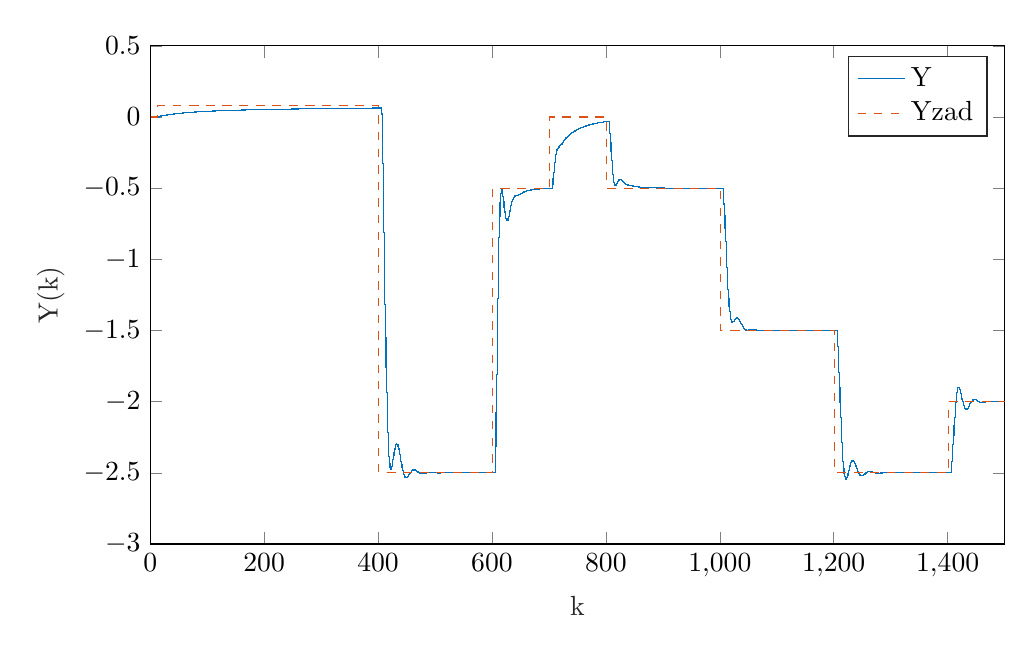
\begin{tikzpicture}

\begin{axis}[%
width=4.272in,
height=2.491in,
at={(0.717in,0.423in)},
scale only axis,
xmin=0,
xmax=1500,
xlabel style={font=\color{white!15!black}},
xlabel={k},
ymin=-3,
ymax=0.5,
ylabel style={font=\color{white!15!black}},
ylabel={Y(k)},
axis background/.style={fill=white},
legend style={legend cell align=left, align=left, draw=white!15!black}
]
\addplot[const plot, color=mycolor1] table[row sep=crcr] {%
1	0\\
2	0\\
3	0\\
4	0\\
5	0\\
6	0\\
7	0\\
8	0\\
9	0\\
10	0\\
11	0\\
12	0\\
13	0\\
14	0\\
15	0\\
16	0\\
17	0.00306636276519328\\
18	0.0069745220336036\\
19	0.00868407348698886\\
20	0.00939627071221701\\
21	0.00979072176544633\\
22	0.010078681316119\\
23	0.0102921949549798\\
24	0.0105809745719523\\
25	0.0110481002860072\\
26	0.0116598934831585\\
27	0.0123520971655962\\
28	0.0130760676877508\\
29	0.0137999724827015\\
30	0.014501457064223\\
31	0.0151698636232913\\
32	0.0158057304964009\\
33	0.0164149627370192\\
34	0.0170041491434318\\
35	0.0175786096279519\\
36	0.0181419339475765\\
37	0.0186959812798714\\
38	0.019241253567623\\
39	0.0197775016269359\\
40	0.0203042543220052\\
41	0.0208211289494967\\
42	0.0213279540711528\\
43	0.0218247784145686\\
44	0.0223118182072475\\
45	0.022789382817075\\
46	0.0232578093287815\\
47	0.0237174204404407\\
48	0.0241685055137608\\
49	0.0246113179960647\\
50	0.0250460817703749\\
51	0.0254730004683287\\
52	0.0258922658514588\\
53	0.0263040634971293\\
54	0.0267085756590521\\
55	0.0271059820219549\\
56	0.0274964592709342\\
57	0.0278801802450853\\
58	0.0282573131688761\\
59	0.0286280211838865\\
60	0.0289924622060213\\
61	0.0293507890284528\\
62	0.0297031495616695\\
63	0.0300496871180187\\
64	0.0303905406814022\\
65	0.0307258451354792\\
66	0.0310557314472272\\
67	0.03138032681515\\
68	0.0316997547949487\\
69	0.0320141354136757\\
70	0.0323235852795165\\
71	0.032628217690544\\
72	0.0329281427430789\\
73	0.0332234674388606\\
74	0.0335142957898284\\
75	0.0338007289195022\\
76	0.0340828651603829\\
77	0.0343608001472036\\
78	0.0346346269061545\\
79	0.0349044359403481\\
80	0.0351703153118268\\
81	0.0354323507203831\\
82	0.035690625579408\\
83	0.0359452210889302\\
84	0.0361962163059734\\
85	0.0364436882123332\\
86	0.0366877117798695\\
87	0.0369283600334059\\
88	0.0371657041113279\\
89	0.0373998133239719\\
90	0.0376307552098966\\
91	0.0378585955901243\\
92	0.038083398620438\\
93	0.0383052268418127\\
94	0.0385241412290606\\
95	0.0387402012377589\\
96	0.0389534648495323\\
97	0.0391639886157543\\
98	0.0393718276997301\\
99	0.0395770359174217\\
100	0.0397796657767718\\
101	0.0399797685156822\\
102	0.0401773941386984\\
103	0.0403725914524512\\
104	0.0405654080999029\\
105	0.0407558905934448\\
106	0.0409440843468894\\
107	0.0411300337063987\\
108	0.0413137819803912\\
109	0.0414953714684635\\
110	0.0416748434893656\\
111	0.0418522384080635\\
112	0.042027595661925\\
113	0.0422009537860596\\
114	0.0423723504378446\\
115	0.0425418224206662\\
116	0.0427094057069064\\
117	0.0428751354602008\\
118	0.0430390460569946\\
119	0.0432011711074236\\
120	0.0433615434755409\\
121	0.0435201952989173\\
122	0.0436771580076331\\
123	0.0438324623426863\\
124	0.0439861383738362\\
125	0.0441382155169024\\
126	0.0442887225505384\\
127	0.0444376876324981\\
128	0.0445851383154127\\
129	0.0447311015620953\\
130	0.0448756037603885\\
131	0.0450186707375715\\
132	0.0451603277743417\\
133	0.0453005996183845\\
134	0.0454395104975461\\
135	0.0455770841326221\\
136	0.0457133437497748\\
137	0.0458483120925917\\
138	0.0459820114337978\\
139	0.0461144635866314\\
140	0.0462456899158965\\
141	0.0463757113487013\\
142	0.0465045483848929\\
143	0.0466322211071988\\
144	0.0467587491910842\\
145	0.0468841488114209\\
146	0.0470084099377715\\
147	0.0471315059032339\\
148	0.0472534219717933\\
149	0.0473741580791551\\
150	0.0474937245213817\\
151	0.0476121375715084\\
152	0.04772941714297\\
153	0.0478455848178707\\
154	0.0479606619236713\\
155	0.0480746688093015\\
156	0.0481876248457121\\
157	0.0482995486426093\\
158	0.048410458226425\\
159	0.0485203711677812\\
160	0.0486293046767021\\
161	0.0487372756429454\\
162	0.048844300637599\\
163	0.0489503959015508\\
164	0.0490555773369254\\
165	0.0491598605048163\\
166	0.0492632606278601\\
167	0.0493657925966762\\
168	0.0494674709786148\\
169	0.0495683100271843\\
170	0.0496683236911051\\
171	0.0497675256226694\\
172	0.0498659291854766\\
173	0.0499635474616785\\
174	0.0500603932588719\\
175	0.0501564791167466\\
176	0.0502518173135597\\
177	0.0503464198724583\\
178	0.0504402985676536\\
179	0.0505334649304386\\
180	0.0506259302550459\\
181	0.0507177056043426\\
182	0.0508088018153655\\
183	0.0508992295046994\\
184	0.050988999073704\\
185	0.0510781207135965\\
186	0.0511666044103926\\
187	0.0512544599497144\\
188	0.0513416969214655\\
189	0.0514283247243811\\
190	0.0515143525704549\\
191	0.0515997894892472\\
192	0.0516846443320777\\
193	0.0517689257761067\\
194	0.0518526423283082\\
195	0.0519358023293376\\
196	0.0520184139572979\\
197	0.0521004852314073\\
198	0.0521820240155712\\
199	0.0522630380218606\\
200	0.0523435348139017\\
201	0.0524235218101772\\
202	0.0525030062872432\\
203	0.0525819953828637\\
204	0.0526604960990657\\
205	0.0527385153051164\\
206	0.0528160597404251\\
207	0.0528931360173725\\
208	0.0529697506240688\\
209	0.0530459099270429\\
210	0.0531216201738652\\
211	0.0531968874957043\\
212	0.0532717179098222\\
213	0.0533461173220064\\
214	0.0534200915289442\\
215	0.0534936462205375\\
216	0.0535667869821623\\
217	0.0536395192968732\\
218	0.0537118485475546\\
219	0.0537837800190203\\
220	0.053855318900063\\
221	0.0539264702854544\\
222	0.053997239177898\\
223	0.0540676304899361\\
224	0.054137649045811\\
225	0.0542072995832828\\
226	0.0542765867554046\\
227	0.0543455151322561\\
228	0.0544140892026375\\
229	0.0544823133757227\\
230	0.0545501919826759\\
231	0.0546177292782297\\
232	0.054684929442228\\
233	0.0547517965811328\\
234	0.054818334729497\\
235	0.0548845478514036\\
236	0.0549504398418727\\
237	0.0550160145282362\\
238	0.0550812756714819\\
239	0.0551462269675675\\
240	0.0552108720487047\\
241	0.0552752144846158\\
242	0.0553392577837612\\
243	0.0554030053945402\\
244	0.0554664607064659\\
245	0.055529627051313\\
246	0.0555925077042418\\
247	0.0556551058848964\\
248	0.0557174247584802\\
249	0.0557794674368066\\
250	0.0558412369793286\\
251	0.0559027363941447\\
252	0.0559639686389839\\
253	0.0560249366221697\\
254	0.0560856432035627\\
255	0.0561460911954841\\
256	0.0562062833636188\\
257	0.0562662224278997\\
258	0.0563259110633728\\
259	0.0563853519010453\\
260	0.0564445475287141\\
261	0.0565035004917785\\
262	0.0565622132940349\\
263	0.0566206883984555\\
264	0.0566789282279507\\
265	0.0567369351661152\\
266	0.0567947115579595\\
267	0.0568522597106255\\
268	0.0569095818940883\\
269	0.0569666803418424\\
270	0.0570235572515753\\
271	0.0570802147858259\\
272	0.0571366550726306\\
273	0.0571928802061559\\
274	0.0572488922473179\\
275	0.0573046932243899\\
276	0.0573602851335973\\
277	0.0574156699397007\\
278	0.057470849576567\\
279	0.0575258259477301\\
280	0.0575806009269389\\
281	0.0576351763586958\\
282	0.0576895540587836\\
283	0.0577437358147823\\
284	0.0577977233865758\\
285	0.0578515185068486\\
286	0.0579051228815721\\
287	0.0579585381904826\\
288	0.0580117660875488\\
289	0.0580648082014306\\
290	0.0581176661359291\\
291	0.0581703414704278\\
292	0.0582228357603252\\
293	0.0582751505374587\\
294	0.0583272873105208\\
295	0.0583792475654674\\
296	0.0584310327659174\\
297	0.0584826443535457\\
298	0.0585340837484678\\
299	0.0585853523496175\\
300	0.0586364515351177\\
301	0.0586873826626433\\
302	0.0587381470697777\\
303	0.058788746074363\\
304	0.0588391809748426\\
305	0.058889453050598\\
306	0.0589395635622794\\
307	0.0589895137521292\\
308	0.0590393048443007\\
309	0.0590889380451696\\
310	0.0591384145436405\\
311	0.0591877355114474\\
312	0.0592369021034485\\
313	0.059285915457916\\
314	0.0593347766968197\\
315	0.059383486926106\\
316	0.0594320472359718\\
317	0.0594804587011329\\
318	0.0595287223810875\\
319	0.0595768393203755\\
320	0.0596248105488321\\
321	0.0596726370818376\\
322	0.0597203199205618\\
323	0.0597678600522051\\
324	0.0598152584502337\\
325	0.0598625160746119\\
326	0.0599096338720294\\
327	0.0599566127761248\\
328	0.0600034537077045\\
329	0.0600501575749588\\
330	0.0600967252736728\\
331	0.0601431576874341\\
332	0.0601894556878374\\
333	0.0602356201346836\\
334	0.0602816518761779\\
335	0.0603275517491216\\
336	0.0603733205791027\\
337	0.0604189591806821\\
338	0.0604644683575761\\
339	0.0605098489028367\\
340	0.0605551015990279\\
341	0.0606002272183991\\
342	0.0606452265230555\\
343	0.0606901002651253\\
344	0.0607348491869243\\
345	0.0607794740211171\\
346	0.0608239754908758\\
347	0.0608683543100359\\
348	0.0609126111832492\\
349	0.0609567468061346\\
350	0.0610007618654253\\
351	0.0610446570391143\\
352	0.061088432996597\\
353	0.0611320903988112\\
354	0.061175629898375\\
355	0.061219052139722\\
356	0.061262357759234\\
357	0.0613055473853722\\
358	0.0613486216388048\\
359	0.0613915811325337\\
360	0.0614344264720185\\
361	0.0614771582552976\\
362	0.0615197770731088\\
363	0.0615622835090063\\
364	0.0616046781394765\\
365	0.0616469615340517\\
366	0.0616891342554215\\
367	0.061731196859543\\
368	0.0617731498957481\\
369	0.0618149939068498\\
370	0.0618567294292466\\
371	0.0618983569930243\\
372	0.0619398771220572\\
373	0.0619812903341069\\
374	0.0620225971409195\\
375	0.062063798048321\\
376	0.0621048935563116\\
377	0.0621458841591579\\
378	0.0621867703454838\\
379	0.0622275525983595\\
380	0.0622682313953895\\
381	0.0623088072087988\\
382	0.0623492805055175\\
383	0.0623896517472645\\
384	0.0624299213906293\\
385	0.0624700898871522\\
386	0.0625101576834043\\
387	0.0625501252210647\\
388	0.0625899929369972\\
389	0.0626297612633258\\
390	0.0626694306275086\\
391	0.0627090014524105\\
392	0.0627484741563747\\
393	0.0627878491532932\\
394	0.062827126852676\\
395	0.062866307659719\\
396	0.0629053919753708\\
397	0.0629443801963986\\
398	0.0629832727154528\\
399	0.0630220699211307\\
400	0.0630607721980388\\
401	0.0630993799268544\\
402	0.0631378934843862\\
403	0.0631763132436335\\
404	0.0632146395738446\\
405	0.0632528728405749\\
406	0.0206679911457022\\
407	-0.126174865629298\\
408	-0.324972430939195\\
409	-0.557153035862454\\
410	-0.810302291612631\\
411	-1.0690634880697\\
412	-1.31868142472533\\
413	-1.54954905035062\\
414	-1.75634606764503\\
415	-1.93682654053666\\
416	-2.08990448198347\\
417	-2.21527063280361\\
418	-2.31351902649671\\
419	-2.38608818481501\\
420	-2.43511332762069\\
421	-2.46329126373204\\
422	-2.47375224420437\\
423	-2.46990901768679\\
424	-2.45528909446455\\
425	-2.43336706325471\\
426	-2.40740997737486\\
427	-2.38034577103653\\
428	-2.35466300771972\\
429	-2.33234696144201\\
430	-2.31485263936797\\
431	-2.30311151722506\\
432	-2.29756619265245\\
433	-2.29822589107693\\
434	-2.30473559158945\\
435	-2.31645218092213\\
436	-2.33252214320739\\
437	-2.35195654273961\\
438	-2.37370024582357\\
439	-2.39669334482445\\
440	-2.4199235555269\\
441	-2.44246896734658\\
442	-2.46353096912535\\
443	-2.48245749447\\
444	-2.49875697181716\\
445	-2.51210356027542\\
446	-2.5223344270987\\
447	-2.52943998912971\\
448	-2.53354820021352\\
449	-2.5349041113344\\
450	-2.5338460453741\\
451	-2.53077979656692\\
452	-2.52615227028127\\
453	-2.52042591172201\\
454	-2.51405513103442\\
455	-2.50746572508239\\
456	-2.50103803934706\\
457	-2.49509432926189\\
458	-2.48989049339644\\
459	-2.4856120842427\\
460	-2.48237427443764\\
461	-2.48022527922149\\
462	-2.4791526151187\\
463	-2.47909150944626\\
464	-2.47993475981427\\
465	-2.48154336885283\\
466	-2.48375733725748\\
467	-2.48640607822649\\
468	-2.48931800975723\\
469	-2.49232898079165\\
470	-2.49528928711754\\
471	-2.49806912893929\\
472	-2.50056245101248\\
473	-2.50268918597796\\
474	-2.50439599047463\\
475	-2.50565562066754\\
476	-2.50646513827377\\
477	-2.50684316961405\\
478	-2.50682645862529\\
479	-2.50646596050214\\
480	-2.50582271649952\\
481	-2.50496373368215\\
482	-2.50395806774132\\
483	-2.50287327445121\\
484	-2.5017723581794\\
485	-2.50071130645466\\
486	-2.49973726021583\\
487	-2.4988873320845\\
488	-2.4981880515527\\
489	-2.49765538766534\\
490	-2.4972952774624\\
491	-2.49710457253063\\
492	-2.49707230648893\\
493	-2.49718118273508\\
494	-2.49740918368077\\
495	-2.49773120917373\\
496	-2.49812066191379\\
497	-2.49855091043616\\
498	-2.49899657469405\\
499	-2.49943459451979\\
500	-2.49984505646122\\
501	-2.50021176897785\\
502	-2.50052258915898\\
503	-2.50076951554972\\
504	-2.50094857102587\\
505	-2.50105950676072\\
506	-2.501105363113\\
507	-2.50109192578393\\
508	-2.50102711598796\\
509	-2.50092035188491\\
510	-2.50078191541995\\
511	-2.50062235434894\\
512	-2.50045194394555\\
513	-2.50028022705716\\
514	-2.50011564514478\\
515	-2.4999652670263\\
516	-2.49983461651551\\
517	-2.49972759523573\\
518	-2.49964649275025\\
519	-2.49959207289998\\
520	-2.49956372292156\\
521	-2.49955965053416\\
522	-2.49957711368209\\
523	-2.49961266791954\\
524	-2.49966241740782\\
525	-2.49972225703416\\
526	-2.49978809511094\\
527	-2.49985604833099\\
528	-2.49992260299955\\
529	-2.49998473890902\\
530	-2.50004001445551\\
531	-2.50008661362537\\
532	-2.50012335723112\\
533	-2.50014968220202\\
534	-2.50016559380409\\
535	-2.50017159637151\\
536	-2.50016860848488\\
537	-2.50015786855788\\
538	-2.50014083653119\\
539	-2.50011909686771\\
540	-2.50009426735032\\
541	-2.50006791735825\\
542	-2.50004149839657\\
543	-2.50001628872731\\
544	-2.49999335304891\\
545	-2.49997351733222\\
546	-2.49995735817993\\
547	-2.4999452054553\\
548	-2.49993715644095\\
549	-2.49993309944603\\
550	-2.49993274457907\\
551	-2.49993565933759\\
552	-2.49994130671948\\
553	-2.49994908371936\\
554	-2.49995835831444\\
555	-2.49996850334753\\
556	-2.49997892605728\\
557	-2.49998909236686\\
558	-2.49999854540198\\
559	-2.50000691805044\\
560	-2.50001393968446\\
561	-2.50001943743237\\
562	-2.5000233326011\\
563	-2.50002563301067\\
564	-2.50002642210545\\
565	-2.500025845757\\
566	-2.50002409767264\\
567	-2.50002140427999\\
568	-2.50001800987716\\
569	-2.50001416272925\\
570	-2.50001010266419\\
571	-2.50000605058116\\
572	-2.50000220014317\\
573	-2.4999987117873\\
574	-2.49999570905854\\
575	-2.49999327716096\\
576	-2.49999146352621\\
577	-2.49999028012694\\
578	-2.49998970721191\\
579	-2.49998969811056\\
580	-2.49999018474647\\
581	-2.49999108350851\\
582	-2.49999230115459\\
583	-2.49999374046015\\
584	-2.49999530537152\\
585	-2.49999690547651\\
586	-2.49999845966085\\
587	-2.49999989887358\\
588	-2.50000116797704\\
589	-2.5000022267038\\
590	-2.50000304978321\\
591	-2.5000036263323\\
592	-2.5000039586298\\
593	-2.50000406040705\\
594	-2.50000395479664\\
595	-2.5000036720789\\
596	-2.50000324735902\\
597	-2.50000271829473\\
598	-2.50000212297762\\
599	-2.50000149805115\\
600	-2.50000087712684\\
601	-2.5000002895387\\
602	-2.49999975945436\\
603	-2.49999930534239\\
604	-2.49999893977806\\
605	-2.49999866955572\\
606	-2.31511721022006\\
607	-2.07340655115093\\
608	-1.81089046113456\\
609	-1.54148048143904\\
610	-1.27693082122322\\
611	-1.04086814665325\\
612	-0.846960356108147\\
613	-0.699652170765926\\
614	-0.597745103091698\\
615	-0.536747172567347\\
616	-0.510022317664309\\
617	-0.509941382174139\\
618	-0.528857043288765\\
619	-0.559700393388257\\
620	-0.59630057626855\\
621	-0.633555180426949\\
622	-0.667508360564888\\
623	-0.695354837369131\\
624	-0.715384606652755\\
625	-0.72688072078524\\
626	-0.729978213725581\\
627	-0.725491579611854\\
628	-0.714721250082666\\
629	-0.699253223025462\\
630	-0.680768149811059\\
631	-0.66087569034423\\
632	-0.640986514865031\\
633	-0.622228652406369\\
634	-0.60540843948652\\
635	-0.591010723804351\\
636	-0.579229314969374\\
637	-0.570017246144755\\
638	-0.563146863297168\\
639	-0.558271418037866\\
640	-0.554982021962013\\
641	-0.552856012321513\\
642	-0.551494684576884\\
643	-0.550549848836133\\
644	-0.549739758882896\\
645	-0.548855692921188\\
646	-0.547760898224357\\
647	-0.546383807605576\\
648	-0.544707444505479\\
649	-0.542756797982353\\
650	-0.540585707184332\\
651	-0.5382644837521\\
652	-0.535869156056266\\
653	-0.533472875053756\\
654	-0.53113970696217\\
655	-0.528920774758319\\
656	-0.526852511755818\\
657	-0.524956660290806\\
658	-0.523241583137107\\
659	-0.521704445254843\\
660	-0.520333856113131\\
661	-0.51911262433054\\
662	-0.518020353690663\\
663	-0.517035691571989\\
664	-0.516138118855203\\
665	-0.515309238467989\\
666	-0.514533574404039\\
667	-0.513798932923784\\
668	-0.513096402979635\\
669	-0.512420085168847\\
670	-0.51176663991955\\
671	-0.511134738753421\\
672	-0.510524490000225\\
673	-0.509936894747488\\
674	-0.509373372232163\\
675	-0.5088353780162\\
676	-0.508324124348514\\
677	-0.507840400845425\\
678	-0.507384485343774\\
679	-0.506956129473683\\
680	-0.506554600882176\\
681	-0.506178763667363\\
682	-0.505827179922186\\
683	-0.505498217786867\\
684	-0.505190154556739\\
685	-0.504901266746435\\
686	-0.504629902225424\\
687	-0.504374532366905\\
688	-0.504133784442013\\
689	-0.503906456179492\\
690	-0.503691515501814\\
691	-0.503488088998178\\
692	-0.503295442791895\\
693	-0.503112959210747\\
694	-0.502940112183547\\
695	-0.502776443666985\\
696	-0.502621542742146\\
697	-0.5024750283798\\
698	-0.502336536307639\\
699	-0.502205709951892\\
700	-0.502082195083906\\
701	-0.501965637579189\\
702	-0.501855683581439\\
703	-0.501751981339909\\
704	-0.501654184034144\\
705	-0.501561952993926\\
706	-0.473183496672882\\
707	-0.433750918161082\\
708	-0.393027221019561\\
709	-0.354023009708238\\
710	-0.318357782951757\\
711	-0.287898844814806\\
712	-0.263550351795986\\
713	-0.245074442738585\\
714	-0.231631969167041\\
715	-0.22215090353935\\
716	-0.215504713025756\\
717	-0.210640945298832\\
718	-0.206682790805213\\
719	-0.202978985229137\\
720	-0.199105986495621\\
721	-0.194837392890037\\
722	-0.190104977877462\\
723	-0.184955190655131\\
724	-0.179504681959246\\
725	-0.173900605069719\\
726	-0.168289646914262\\
727	-0.162797129073356\\
728	-0.157515727288847\\
729	-0.152502340764845\\
730	-0.147781000271226\\
731	-0.143349480603494\\
732	-0.139187476024714\\
733	-0.135264658982466\\
734	-0.131547502590312\\
735	-0.128004289083587\\
736	-0.124608179251416\\
737	-0.121338543893032\\
738	-0.118180949060649\\
739	-0.115126257035069\\
740	-0.112169282971125\\
741	-0.109307365867517\\
742	-0.106539103320001\\
743	-0.103863388218272\\
744	-0.101278790172197\\
745	-0.0987832547759485\\
746	-0.0963740523600195\\
747	-0.0940478917983003\\
748	-0.0918011182072212\\
749	-0.0896299288172071\\
750	-0.0875305621503629\\
751	-0.0854994365468782\\
752	-0.0835332315232939\\
753	-0.0816289177003198\\
754	-0.0797837478668801\\
755	-0.0779952239215106\\
756	-0.0762610532511201\\
757	-0.0745791049888731\\
758	-0.0729473727868477\\
759	-0.0713639471663391\\
760	-0.0698269977164887\\
761	-0.0683347636102229\\
762	-0.0668855500515871\\
763	-0.0654777281626117\\
764	-0.0641097362005581\\
765	-0.0627800806150296\\
766	-0.0614873361071592\\
767	-0.0602301444071684\\
768	-0.0590072118772805\\
769	-0.0578173062641697\\
770	-0.0566592529948675\\
771	-0.0555319313760505\\
772	-0.0544342709654659\\
773	-0.0533652482754347\\
774	-0.0523238838696108\\
775	-0.0513092398405679\\
776	-0.0503204176117768\\
777	-0.0493565559901482\\
778	-0.0484168293975938\\
779	-0.0475004462239258\\
780	-0.0466066472617163\\
781	-0.0457347042012318\\
782	-0.044883918177224\\
783	-0.0440536183681136\\
784	-0.0432431606522476\\
785	-0.0424519263265392\\
786	-0.0416793208912523\\
787	-0.0409247729022185\\
788	-0.0401877328892885\\
789	-0.0394676723378825\\
790	-0.038764082729327\\
791	-0.0380764746352224\\
792	-0.0374043768612129\\
793	-0.0367473356360053\\
794	-0.0361049138421017\\
795	-0.0354766902853278\\
796	-0.0348622590007531\\
797	-0.0342612285929756\\
798	-0.0336732216089974\\
799	-0.033097873942057\\
800	-0.0325348342648661\\
801	-0.0319837634907368\\
802	-0.0314443342611252\\
803	-0.0309162304581519\\
804	-0.0303991467407186\\
805	-0.0298927881029035\\
806	-0.0573919072667449\\
807	-0.113730139804285\\
808	-0.179418407988437\\
809	-0.245591369076659\\
810	-0.307453477655957\\
811	-0.361689743405049\\
812	-0.405798566323478\\
813	-0.438829374154483\\
814	-0.461151332998219\\
815	-0.473964187382439\\
816	-0.478962679710727\\
817	-0.478093740508417\\
818	-0.473327054481166\\
819	-0.466460962443812\\
820	-0.458994845286614\\
821	-0.452066872894868\\
822	-0.446444006076616\\
823	-0.442550917504561\\
824	-0.44052453582119\\
825	-0.440281227734948\\
826	-0.441585910233553\\
827	-0.444115667665202\\
828	-0.447513472492037\\
829	-0.45142997013808\\
830	-0.455553019423499\\
831	-0.459625861269339\\
832	-0.463455506475912\\
833	-0.466913294106162\\
834	-0.469929674802797\\
835	-0.472485193913564\\
836	-0.474599443198868\\
837	-0.476319461583019\\
838	-0.477708733016324\\
839	-0.478837586301627\\
840	-0.47977547591621\\
841	-0.480585336582511\\
842	-0.481319972586649\\
843	-0.482020272917682\\
844	-0.482714935321715\\
845	-0.483421330624862\\
846	-0.484147133508409\\
847	-0.484892375653031\\
848	-0.485651629873826\\
849	-0.486416098642792\\
850	-0.487175448178571\\
851	-0.487919293217989\\
852	-0.488638293038599\\
853	-0.489324863661236\\
854	-0.489973543490842\\
855	-0.490581070309505\\
856	-0.491146237782194\\
857	-0.491669601294686\\
858	-0.492153098094451\\
859	-0.492599637446407\\
860	-0.493012704782691\\
861	-0.493396011271882\\
862	-0.493753208160524\\
863	-0.494087674576661\\
864	-0.494402378800631\\
865	-0.494699806554277\\
866	-0.494981945628484\\
867	-0.495250313960657\\
868	-0.495506017762422\\
869	-0.495749827092535\\
870	-0.495982257965594\\
871	-0.496203652303783\\
872	-0.496414249448571\\
873	-0.496614245291478\\
874	-0.496803837170114\\
875	-0.4969832543903\\
876	-0.49715277552292\\
877	-0.497312734481698\\
878	-0.497463517850792\\
879	-0.497605556059347\\
880	-0.497739310868556\\
881	-0.49786526132316\\
882	-0.497983889897791\\
883	-0.498095670103559\\
884	-0.498201056363596\\
885	-0.498300476555778\\
886	-0.498394327280634\\
887	-0.498482971654331\\
888	-0.498566739252236\\
889	-0.498645927731719\\
890	-0.498720805632276\\
891	-0.498791615872429\\
892	-0.498858579521058\\
893	-0.498921899501331\\
894	-0.498981763975443\\
895	-0.499038349247682\\
896	-0.499091822104168\\
897	-0.499142341575183\\
898	-0.4991900601576\\
899	-0.499235124570298\\
900	-0.499277676135453\\
901	-0.499317850885509\\
902	-0.499355779492161\\
903	-0.499391587102747\\
904	-0.499425393153938\\
905	-0.499457311215027\\
906	-0.499487448895531\\
907	-0.499515907835795\\
908	-0.499542783785731\\
909	-0.499568166766444\\
910	-0.499592141302225\\
911	-0.499614786706172\\
912	-0.499636177401115\\
913	-0.499656383257949\\
914	-0.499675469935496\\
915	-0.499693499208907\\
916	-0.499710529277009\\
917	-0.499726615042375\\
918	-0.499741808361063\\
919	-0.499756158261561\\
920	-0.499769711134584\\
921	-0.499782510896747\\
922	-0.499794599132014\\
923	-0.499806015215109\\
924	-0.49981679642101\\
925	-0.499826978024227\\
926	-0.49983659339099\\
927	-0.499845674066773\\
928	-0.499854249860908\\
929	-0.499862348929383\\
930	-0.499869997856367\\
931	-0.499877221734584\\
932	-0.499884044244334\\
933	-0.499890487730759\\
934	-0.499896573278901\\
935	-0.49990232078603\\
936	-0.499907749030838\\
937	-0.499912875739149\\
938	-0.499917717645934\\
939	-0.499922290553539\\
940	-0.499926609386127\\
941	-0.499930688240469\\
942	-0.499934540433257\\
943	-0.499938178545183\\
944	-0.499941614462045\\
945	-0.499944859413174\\
946	-0.499947924007422\\
947	-0.49995081826699\\
948	-0.499953551659289\\
949	-0.499956133127054\\
950	-0.499958571116832\\
951	-0.499960873606014\\
952	-0.499963048128476\\
953	-0.499965101798937\\
954	-0.499967041336079\\
955	-0.499968873084489\\
956	-0.499970603035467\\
957	-0.499972236846734\\
958	-0.499973779861092\\
959	-0.499975237124047\\
960	-0.499976613400474\\
961	-0.499977913190328\\
962	-0.499979140743473\\
963	-0.499980300073657\\
964	-0.499981394971689\\
965	-0.49998242901786\\
966	-0.499983405593649\\
967	-0.49998432789277\\
968	-0.499985198931587\\
969	-0.499986021558944\\
970	-0.499986798465449\\
971	-0.499987532192238\\
972	-0.499988225139257\\
973	-0.499988879573083\\
974	-0.499989497634323\\
975	-0.499990081344601\\
976	-0.49999063261316\\
977	-0.499991153243109\\
978	-0.499991644937319\\
979	-0.499992109303995\\
980	-0.499992547861945\\
981	-0.499992962045551\\
982	-0.499993353209464\\
983	-0.499993722633045\\
984	-0.499994071524549\\
985	-0.499994401025082\\
986	-0.499994712212334\\
987	-0.499995006104106\\
988	-0.499995283661637\\
989	-0.49999554579275\\
990	-0.499995793354818\\
991	-0.499996027157567\\
992	-0.499996247965725\\
993	-0.49999645650152\\
994	-0.49999665344704\\
995	-0.499996839446465\\
996	-0.499997015108173\\
997	-0.499997181006729\\
998	-0.499997337684763\\
999	-0.499997485654745\\
1000	-0.499997625400663\\
1001	-0.499997757379602\\
1002	-0.499997882023245\\
1003	-0.499997999739281\\
1004	-0.49999811091274\\
1005	-0.49999821590725\\
1006	-0.540999558510631\\
1007	-0.611611468623457\\
1008	-0.694460509089916\\
1009	-0.784345302111799\\
1010	-0.877837489856454\\
1011	-0.970935711386462\\
1012	-1.05971733983228\\
1013	-1.14138288711786\\
1014	-1.21405749414418\\
1015	-1.27653911762264\\
1016	-1.3282419575366\\
1017	-1.36916852126562\\
1018	-1.39982800521772\\
1019	-1.42113082405759\\
1020	-1.43428448134051\\
1021	-1.44069062302899\\
1022	-1.44184332660564\\
1023	-1.43923434929244\\
1024	-1.434271382988\\
1025	-1.42821308994332\\
1026	-1.42212285413639\\
1027	-1.4168416755439\\
1028	-1.41297910853174\\
1029	-1.4109198463482\\
1030	-1.41084273819385\\
1031	-1.41274870797376\\
1032	-1.41649412032246\\
1033	-1.42182649072542\\
1034	-1.42841994937273\\
1035	-1.43590844373635\\
1036	-1.44391522974676\\
1037	-1.45207771242731\\
1038	-1.46006713447452\\
1039	-1.46760297183701\\
1040	-1.47446218377201\\
1041	-1.48048368949096\\
1042	-1.48556861268894\\
1043	-1.48967695560624\\
1044	-1.49282144031968\\
1045	-1.49505928967664\\
1046	-1.49648271605307\\
1047	-1.49720884578771\\
1048	-1.49736973484227\\
1049	-1.49710303277052\\
1050	-1.49654373487291\\
1051	-1.49581733501212\\
1052	-1.49503456285953\\
1053	-1.49428776768433\\
1054	-1.4936489032144\\
1055	-1.49316897972391\\
1056	-1.49287878331353\\
1057	-1.49279061919314\\
1058	-1.49290081465194\\
1059	-1.49319271587921\\
1060	-1.49363992752047\\
1061	-1.4942095709934\\
1062	-1.49486537325485\\
1063	-1.49557043824602\\
1064	-1.49628959541886\\
1065	-1.49699126086911\\
1066	-1.49764878455322\\
1067	-1.49824129029308\\
1068	-1.49875404274798\\
1069	-1.49917839670596\\
1070	-1.49951139877621\\
1071	-1.49975512006593\\
1072	-1.49991580119938\\
1073	-1.50000288881077\\
1074	-1.50002803630134\\
1075	-1.50000413217419\\
1076	-1.4999444076594\\
1077	-1.49986166259937\\
1078	-1.49976763558481\\
1079	-1.49967253189903\\
1080	-1.49958471157654\\
1081	-1.49951053027907\\
1082	-1.49945431803729\\
1083	-1.4994184753355\\
1084	-1.49940366252144\\
1085	-1.49940905697476\\
1086	-1.49943265264199\\
1087	-1.49947157815556\\
1088	-1.49952241247474\\
1089	-1.49958148048088\\
1090	-1.49964511490291\\
1091	-1.49970987504206\\
1092	-1.49977271674984\\
1093	-1.49983111177917\\
1094	-1.49988311781794\\
1095	-1.49992740312007\\
1096	-1.4999632316178\\
1097	-1.49999041571736\\
1098	-1.50000924467867\\
1099	-1.50002039661539\\
1100	-1.50002484180645\\
1101	-1.50002374428045\\
1102	-1.50001836762209\\
1103	-1.50000998975812\\
1104	-1.49999983020569\\
1105	-1.4999889919949\\
1106	-1.49997841928169\\
1107	-1.49996887060365\\
1108	-1.4999609068405\\
1109	-1.49995489224517\\
1110	-1.49995100642101\\
1111	-1.49994926483007\\
1112	-1.49994954531156\\
1113	-1.49995161814554\\
1114	-1.49995517738538\\
1115	-1.49995987147117\\
1116	-1.49996533149354\\
1117	-1.49997119587061\\
1118	-1.49997713060276\\
1119	-1.49998284465579\\
1120	-1.49998810037273\\
1121	-1.49999271911526\\
1122	-1.49999658257597\\
1123	-1.49999963038039\\
1124	-1.50000185471105\\
1125	-1.50000329273973\\
1126	-1.50000401765383\\
1127	-1.50000412901802\\
1128	-1.50000374313228\\
1129	-1.50000298394168\\
1130	-1.50000197493349\\
1131	-1.5000008323306\\
1132	-1.49999965976684\\
1133	-1.49999854451507\\
1134	-1.49999755523835\\
1135	-1.49999674115201\\
1136	-1.49999613242122\\
1137	-1.49999574157555\\
1138	-1.49999556569877\\
1139	-1.49999558914566\\
1140	-1.49999578654724\\
1141	-1.499996125887\\
1142	-1.49999657146125\\
1143	-1.49999708657309\\
1144	-1.49999763584854\\
1145	-1.49999818710294\\
1146	-1.49999871272266\\
1147	-1.4999991905606\\
1148	-1.49999960437205\\
1149	-1.49999994383937\\
1150	-1.50000020425\\
1151	-1.50000038590167\\
1152	-1.50000049331266\\
1153	-1.5000005343136\\
1154	-1.50000051909198\\
1155	-1.50000045925186\\
1156	-1.50000036694031\\
1157	-1.50000025408037\\
1158	-1.50000013173751\\
1159	-1.50000000963478\\
1160	-1.49999989582099\\
1161	-1.49999979648656\\
1162	-1.49999971591418\\
1163	-1.49999965654583\\
1164	-1.49999961914377\\
1165	-1.49999960302142\\
1166	-1.49999960631983\\
1167	-1.49999962630673\\
1168	-1.49999965967743\\
1169	-1.49999970284014\\
1170	-1.49999975217182\\
1171	-1.49999980423472\\
1172	-1.49999985594741\\
1173	-1.49999990470786\\
1174	-1.49999994846909\\
1175	-1.49999998577077\\
1176	-1.50000001573187\\
1177	-1.50000003801107\\
1178	-1.50000005274233\\
1179	-1.50000006045336\\
1180	-1.50000006197429\\
1181	-1.50000005834338\\
1182	-1.50000005071576\\
1183	-1.50000004027983\\
1184	-1.50000002818494\\
1185	-1.50000001548277\\
1186	-1.50000000308351\\
1187	-1.49999999172708\\
1188	-1.49999998196856\\
1189	-1.49999997417649\\
1190	-1.4999999685421\\
1191	-1.49999996509714\\
1192	-1.49999996373792\\
1193	-1.49999996425334\\
1194	-1.49999996635444\\
1195	-1.49999996970379\\
1196	-1.49999997394284\\
1197	-1.49999997871618\\
1198	-1.49999998369164\\
1199	-1.49999998857593\\
1200	-1.49999999312541\\
1201	-1.49999999715245\\
1202	-1.50000000052736\\
1203	-1.50000000317682\\
1204	-1.50000000507924\\
1205	-1.50000000625792\\
1206	-1.54222914338483\\
1207	-1.61419641298736\\
1208	-1.70079314783355\\
1209	-1.79795344235157\\
1210	-1.90261107776476\\
1211	-2.00871552689938\\
1212	-2.11046219485877\\
1213	-2.20415365752577\\
1214	-2.28778524177118\\
1215	-2.3601408641529\\
1216	-2.42042634861459\\
1217	-2.46834030261127\\
1218	-2.50408794532772\\
1219	-2.52831080576179\\
1220	-2.54201053215751\\
1221	-2.54648008895384\\
1222	-2.54322737551831\\
1223	-2.53388997304847\\
1224	-2.52014884610654\\
1225	-2.50364719643551\\
1226	-2.48591845171824\\
1227	-2.46832677040214\\
1228	-2.45202269144254\\
1229	-2.43791516098304\\
1230	-2.4266597009349\\
1231	-2.41866131100542\\
1232	-2.41408987023388\\
1233	-2.41290531867799\\
1234	-2.41488973660183\\
1235	-2.41968354106282\\
1236	-2.42682330450141\\
1237	-2.43577908493253\\
1238	-2.44598957811371\\
1239	-2.45689381413405\\
1240	-2.46795849787301\\
1241	-2.47870042303729\\
1242	-2.48870367158721\\
1243	-2.49763154873429\\
1244	-2.50523340494692\\
1245	-2.51134666678144\\
1246	-2.51589454217478\\
1247	-2.51887998481502\\
1248	-2.52037659558846\\
1249	-2.5205172043434\\
1250	-2.51948090907626\\
1251	-2.51747934944045\\
1252	-2.51474295617875\\
1253	-2.51150784912957\\
1254	-2.50800395808109\\
1255	-2.50444481973327\\
1256	-2.50101936904331\\
1257	-2.49788590382538\\
1258	-2.49516826699204\\
1259	-2.49295416940685\\
1260	-2.49129547419121\\
1261	-2.49021018442592\\
1262	-2.48968582211894\\
1263	-2.48968385662074\\
1264	-2.49014483328076\\
1265	-2.49099386487255\\
1266	-2.49214617539745\\
1267	-2.4935124243658\\
1268	-2.49500358576655\\
1269	-2.49653520624426\\
1270	-2.49803091855149\\
1271	-2.49942513667096\\
1272	-2.5006649061266\\
1273	-2.50171092538012\\
1274	-2.50253779068946\\
1275	-2.50313354658624\\
1276	-2.50349864673401\\
1277	-2.50364444518461\\
1278	-2.50359134607232\\
1279	-2.50336674096856\\
1280	-2.50300285810839\\
1281	-2.50253463736232\\
1282	-2.50199773020187\\
1283	-2.50142670615382\\
1284	-2.50085352756112\\
1285	-2.50030633405829\\
1286	-2.49980855812952\\
1287	-2.49937837441718\\
1288	-2.49902846887234\\
1289	-2.49876609996957\\
1290	-2.49859341341084\\
1291	-2.49850796417755\\
1292	-2.4985033954234\\
1293	-2.49857022234275\\
1294	-2.49869667048027\\
1295	-2.49886952155578\\
1296	-2.49907492529685\\
1297	-2.49929914250639\\
1298	-2.49952919215449\\
1299	-2.49975338320791\\
1300	-2.49996171977664\\
1301	-2.50014617560141\\
1302	-2.50030084062976\\
1303	-2.50042194820439\\
1304	-2.50050779605776\\
1305	-2.50055857778633\\
1306	-2.50057614374302\\
1307	-2.50056371137638\\
1308	-2.50052554504681\\
1309	-2.50046662439334\\
1310	-2.50039231856826\\
1311	-2.50030808128054\\
1312	-2.5002191787808\\
1313	-2.50013045986651\\
1314	-2.50004617386433\\
1315	-2.49996983951484\\
1316	-2.49990416487979\\
1317	-2.49985101592205\\
1318	-2.49981142935156\\
1319	-2.49978566373729\\
1320	-2.49977328177462\\
1321	-2.49977325596563\\
1322	-2.499784089787\\
1323	-2.49980394664153\\
1324	-2.49983077945364\\
1325	-2.4998624546078\\
1326	-2.49989686496765\\
1327	-2.4999320278783\\
1328	-2.49996616527352\\
1329	-2.49999776421842\\
1330	-2.50002561736017\\
1331	-2.50004884378713\\
1332	-2.50006689167638\\
1333	-2.50007952481584\\
1334	-2.50008679560726\\
1335	-2.50008900748922\\
1336	-2.50008666986982\\
1337	-2.50008044864321\\
1338	-2.50007111520298\\
1339	-2.50005949658358\\
1340	-2.50004642898751\\
1341	-2.50003271651894\\
1342	-2.50001909647316\\
1343	-2.50000621205257\\
1344	-2.49999459291721\\
1345	-2.49998464355178\\
1346	-2.49997663905808\\
1347	-2.49997072767232\\
1348	-2.49996693906908\\
1349	-2.49996519734964\\
1350	-2.49996533752146\\
1351	-2.49996712425308\\
1352	-2.49997027172706\\
1353	-2.49997446350407\\
1354	-2.49997937144294\\
1355	-2.49998467288273\\
1356	-2.49999006547308\\
1357	-2.49999527922651\\
1358	-2.50000008555153\\
1359	-2.50000430319981\\
1360	-2.50000780121695\\
1361	-2.50001049911922\\
1362	-2.500012364625\\
1363	-2.50001340934716\\
1364	-2.50001368290081\\
1365	-2.50001326590228\\
1366	-2.50001226233004\\
1367	-2.50001079169212\\
1368	-2.5000089813997\\
1369	-2.5000069596879\\
1370	-2.50000484935752\\
1371	-2.50000276253831\\
1372	-2.50000079660108\\
1373	-2.49999903127561\\
1374	-2.49999752696584\\
1375	-2.49999632419812\\
1376	-2.49999544409098\\
1377	-2.49999488969991\\
1378	-2.49999464806616\\
1379	-2.4999946927855\\
1380	-2.4999949869106\\
1381	-2.49999548600682\\
1382	-2.49999614119626\\
1383	-2.49999690204513\\
1384	-2.49999771917495\\
1385	-2.49999854650568\\
1386	-2.49999934306777\\
1387	-2.50000007434858\\
1388	-2.50000071316507\\
1389	-2.50000124007839\\
1390	-2.50000164338621\\
1391	-2.50000191874439\\
1392	-2.50000206848132\\
1393	-2.50000210067512\\
1394	-2.5000020280669\\
1395	-2.50000186688208\\
1396	-2.50000163562779\\
1397	-2.5000013539267\\
1398	-2.50000104143912\\
1399	-2.50000071691425\\
1400	-2.5000003974005\\
1401	-2.5000000976335\\
1402	-2.49999982960954\\
1403	-2.49999960234237\\
1404	-2.49999942179287\\
1405	-2.49999929095384\\
1406	-2.47006432185172\\
1407	-2.42239796304751\\
1408	-2.36578369372532\\
1409	-2.30327377645666\\
1410	-2.23723076059105\\
1411	-2.17124283510389\\
1412	-2.10872914645405\\
1413	-2.05224329284978\\
1414	-2.00361214885652\\
1415	-1.96404361265878\\
1416	-1.93411959796175\\
1417	-1.91382750752003\\
1418	-1.90265547312795\\
1419	-1.89970473370391\\
1420	-1.90379803464037\\
1421	-1.91358244896228\\
1422	-1.92762449447989\\
1423	-1.94449349744895\\
1424	-1.96283091547716\\
1425	-1.98140526252709\\
1426	-1.99915300174643\\
1427	-2.01520601355418\\
1428	-2.02890648856049\\
1429	-2.03981032718242\\
1430	-2.04768030918715\\
1431	-2.0524704608692\\
1432	-2.05430321780307\\
1433	-2.05344114146958\\
1434	-2.05025506741454\\
1435	-2.04519061103332\\
1436	-2.03873491125753\\
1437	-2.03138534005983\\
1438	-2.02362164970811\\
1439	-2.01588268894682\\
1440	-2.0085484251928\\
1441	-2.00192760038823\\
1442	-1.99625096106625\\
1443	-1.99166966989581\\
1444	-1.98825824770643\\
1445	-1.98602122138042\\
1446	-1.98490256302214\\
1447	-1.98479699033092\\
1448	-1.9855622430304\\
1449	-1.98703153954176\\
1450	-1.98902553629778\\
1451	-1.99136324563196\\
1452	-1.99387150619082\\
1453	-1.99639273422407\\
1454	-1.99879080926358\\
1455	-2.00095505989705\\
1456	-2.0028024122653\\
1457	-2.00427784421439\\
1458	-2.0053533510199\\
1459	-2.00602567406426\\
1460	-2.00631307201827\\
1461	-2.00625142564087\\
1462	-2.0058899634536\\
1463	-2.00528687797999\\
1464	-2.00450507318266\\
1465	-2.00360824582152\\
1466	-2.00265745961077\\
1467	-2.00170832428391\\
1468	-2.00080884488813\\
1469	-1.99999796243091\\
1470	-1.99930476754829\\
1471	-1.99874833575661\\
1472	-1.99833810708981\\
1473	-1.99807471492863\\
1474	-1.99795115848302\\
1475	-1.9979542101488\\
1476	-1.99806595194799\\
1477	-1.9982653433906\\
1478	-1.9985297351637\\
1479	-1.99883625784125\\
1480	-1.99916303114553\\
1481	-1.99949015611327\\
1482	-1.9998004689022\\
1483	-2.0000800501524\\
1484	-2.00031849720095\\
1485	-2.00050897761638\\
1486	-2.00064809121888\\
1487	-2.00073557388162\\
1488	-2.00077388000646\\
1489	-2.0007676817913\\
1490	-2.0007233225095\\
1491	-2.00064825833215\\
1492	-2.000550519117\\
1493	-2.00043821346374\\
1494	-2.0003190975942\\
1495	-2.00020022163951\\
1496	-2.00008766104655\\
1497	-1.99998633534538\\
1498	-1.99989991168019\\
1499	-1.9998307864648\\
1500	-1.99978013538275\\
};
\addlegendentry{Y}

\addplot[const plot, color=mycolor2, dashed] table[row sep=crcr] {%
1	0\\
2	0\\
3	0\\
4	0\\
5	0\\
6	0\\
7	0\\
8	0\\
9	0\\
10	0\\
11	0\\
12	0.08\\
13	0.08\\
14	0.08\\
15	0.08\\
16	0.08\\
17	0.08\\
18	0.08\\
19	0.08\\
20	0.08\\
21	0.08\\
22	0.08\\
23	0.08\\
24	0.08\\
25	0.08\\
26	0.08\\
27	0.08\\
28	0.08\\
29	0.08\\
30	0.08\\
31	0.08\\
32	0.08\\
33	0.08\\
34	0.08\\
35	0.08\\
36	0.08\\
37	0.08\\
38	0.08\\
39	0.08\\
40	0.08\\
41	0.08\\
42	0.08\\
43	0.08\\
44	0.08\\
45	0.08\\
46	0.08\\
47	0.08\\
48	0.08\\
49	0.08\\
50	0.08\\
51	0.08\\
52	0.08\\
53	0.08\\
54	0.08\\
55	0.08\\
56	0.08\\
57	0.08\\
58	0.08\\
59	0.08\\
60	0.08\\
61	0.08\\
62	0.08\\
63	0.08\\
64	0.08\\
65	0.08\\
66	0.08\\
67	0.08\\
68	0.08\\
69	0.08\\
70	0.08\\
71	0.08\\
72	0.08\\
73	0.08\\
74	0.08\\
75	0.08\\
76	0.08\\
77	0.08\\
78	0.08\\
79	0.08\\
80	0.08\\
81	0.08\\
82	0.08\\
83	0.08\\
84	0.08\\
85	0.08\\
86	0.08\\
87	0.08\\
88	0.08\\
89	0.08\\
90	0.08\\
91	0.08\\
92	0.08\\
93	0.08\\
94	0.08\\
95	0.08\\
96	0.08\\
97	0.08\\
98	0.08\\
99	0.08\\
100	0.08\\
101	0.08\\
102	0.08\\
103	0.08\\
104	0.08\\
105	0.08\\
106	0.08\\
107	0.08\\
108	0.08\\
109	0.08\\
110	0.08\\
111	0.08\\
112	0.08\\
113	0.08\\
114	0.08\\
115	0.08\\
116	0.08\\
117	0.08\\
118	0.08\\
119	0.08\\
120	0.08\\
121	0.08\\
122	0.08\\
123	0.08\\
124	0.08\\
125	0.08\\
126	0.08\\
127	0.08\\
128	0.08\\
129	0.08\\
130	0.08\\
131	0.08\\
132	0.08\\
133	0.08\\
134	0.08\\
135	0.08\\
136	0.08\\
137	0.08\\
138	0.08\\
139	0.08\\
140	0.08\\
141	0.08\\
142	0.08\\
143	0.08\\
144	0.08\\
145	0.08\\
146	0.08\\
147	0.08\\
148	0.08\\
149	0.08\\
150	0.08\\
151	0.08\\
152	0.08\\
153	0.08\\
154	0.08\\
155	0.08\\
156	0.08\\
157	0.08\\
158	0.08\\
159	0.08\\
160	0.08\\
161	0.08\\
162	0.08\\
163	0.08\\
164	0.08\\
165	0.08\\
166	0.08\\
167	0.08\\
168	0.08\\
169	0.08\\
170	0.08\\
171	0.08\\
172	0.08\\
173	0.08\\
174	0.08\\
175	0.08\\
176	0.08\\
177	0.08\\
178	0.08\\
179	0.08\\
180	0.08\\
181	0.08\\
182	0.08\\
183	0.08\\
184	0.08\\
185	0.08\\
186	0.08\\
187	0.08\\
188	0.08\\
189	0.08\\
190	0.08\\
191	0.08\\
192	0.08\\
193	0.08\\
194	0.08\\
195	0.08\\
196	0.08\\
197	0.08\\
198	0.08\\
199	0.08\\
200	0.08\\
201	0.08\\
202	0.08\\
203	0.08\\
204	0.08\\
205	0.08\\
206	0.08\\
207	0.08\\
208	0.08\\
209	0.08\\
210	0.08\\
211	0.08\\
212	0.08\\
213	0.08\\
214	0.08\\
215	0.08\\
216	0.08\\
217	0.08\\
218	0.08\\
219	0.08\\
220	0.08\\
221	0.08\\
222	0.08\\
223	0.08\\
224	0.08\\
225	0.08\\
226	0.08\\
227	0.08\\
228	0.08\\
229	0.08\\
230	0.08\\
231	0.08\\
232	0.08\\
233	0.08\\
234	0.08\\
235	0.08\\
236	0.08\\
237	0.08\\
238	0.08\\
239	0.08\\
240	0.08\\
241	0.08\\
242	0.08\\
243	0.08\\
244	0.08\\
245	0.08\\
246	0.08\\
247	0.08\\
248	0.08\\
249	0.08\\
250	0.08\\
251	0.08\\
252	0.08\\
253	0.08\\
254	0.08\\
255	0.08\\
256	0.08\\
257	0.08\\
258	0.08\\
259	0.08\\
260	0.08\\
261	0.08\\
262	0.08\\
263	0.08\\
264	0.08\\
265	0.08\\
266	0.08\\
267	0.08\\
268	0.08\\
269	0.08\\
270	0.08\\
271	0.08\\
272	0.08\\
273	0.08\\
274	0.08\\
275	0.08\\
276	0.08\\
277	0.08\\
278	0.08\\
279	0.08\\
280	0.08\\
281	0.08\\
282	0.08\\
283	0.08\\
284	0.08\\
285	0.08\\
286	0.08\\
287	0.08\\
288	0.08\\
289	0.08\\
290	0.08\\
291	0.08\\
292	0.08\\
293	0.08\\
294	0.08\\
295	0.08\\
296	0.08\\
297	0.08\\
298	0.08\\
299	0.08\\
300	0.08\\
301	0.08\\
302	0.08\\
303	0.08\\
304	0.08\\
305	0.08\\
306	0.08\\
307	0.08\\
308	0.08\\
309	0.08\\
310	0.08\\
311	0.08\\
312	0.08\\
313	0.08\\
314	0.08\\
315	0.08\\
316	0.08\\
317	0.08\\
318	0.08\\
319	0.08\\
320	0.08\\
321	0.08\\
322	0.08\\
323	0.08\\
324	0.08\\
325	0.08\\
326	0.08\\
327	0.08\\
328	0.08\\
329	0.08\\
330	0.08\\
331	0.08\\
332	0.08\\
333	0.08\\
334	0.08\\
335	0.08\\
336	0.08\\
337	0.08\\
338	0.08\\
339	0.08\\
340	0.08\\
341	0.08\\
342	0.08\\
343	0.08\\
344	0.08\\
345	0.08\\
346	0.08\\
347	0.08\\
348	0.08\\
349	0.08\\
350	0.08\\
351	0.08\\
352	0.08\\
353	0.08\\
354	0.08\\
355	0.08\\
356	0.08\\
357	0.08\\
358	0.08\\
359	0.08\\
360	0.08\\
361	0.08\\
362	0.08\\
363	0.08\\
364	0.08\\
365	0.08\\
366	0.08\\
367	0.08\\
368	0.08\\
369	0.08\\
370	0.08\\
371	0.08\\
372	0.08\\
373	0.08\\
374	0.08\\
375	0.08\\
376	0.08\\
377	0.08\\
378	0.08\\
379	0.08\\
380	0.08\\
381	0.08\\
382	0.08\\
383	0.08\\
384	0.08\\
385	0.08\\
386	0.08\\
387	0.08\\
388	0.08\\
389	0.08\\
390	0.08\\
391	0.08\\
392	0.08\\
393	0.08\\
394	0.08\\
395	0.08\\
396	0.08\\
397	0.08\\
398	0.08\\
399	0.08\\
400	0.08\\
401	-2.5\\
402	-2.5\\
403	-2.5\\
404	-2.5\\
405	-2.5\\
406	-2.5\\
407	-2.5\\
408	-2.5\\
409	-2.5\\
410	-2.5\\
411	-2.5\\
412	-2.5\\
413	-2.5\\
414	-2.5\\
415	-2.5\\
416	-2.5\\
417	-2.5\\
418	-2.5\\
419	-2.5\\
420	-2.5\\
421	-2.5\\
422	-2.5\\
423	-2.5\\
424	-2.5\\
425	-2.5\\
426	-2.5\\
427	-2.5\\
428	-2.5\\
429	-2.5\\
430	-2.5\\
431	-2.5\\
432	-2.5\\
433	-2.5\\
434	-2.5\\
435	-2.5\\
436	-2.5\\
437	-2.5\\
438	-2.5\\
439	-2.5\\
440	-2.5\\
441	-2.5\\
442	-2.5\\
443	-2.5\\
444	-2.5\\
445	-2.5\\
446	-2.5\\
447	-2.5\\
448	-2.5\\
449	-2.5\\
450	-2.5\\
451	-2.5\\
452	-2.5\\
453	-2.5\\
454	-2.5\\
455	-2.5\\
456	-2.5\\
457	-2.5\\
458	-2.5\\
459	-2.5\\
460	-2.5\\
461	-2.5\\
462	-2.5\\
463	-2.5\\
464	-2.5\\
465	-2.5\\
466	-2.5\\
467	-2.5\\
468	-2.5\\
469	-2.5\\
470	-2.5\\
471	-2.5\\
472	-2.5\\
473	-2.5\\
474	-2.5\\
475	-2.5\\
476	-2.5\\
477	-2.5\\
478	-2.5\\
479	-2.5\\
480	-2.5\\
481	-2.5\\
482	-2.5\\
483	-2.5\\
484	-2.5\\
485	-2.5\\
486	-2.5\\
487	-2.5\\
488	-2.5\\
489	-2.5\\
490	-2.5\\
491	-2.5\\
492	-2.5\\
493	-2.5\\
494	-2.5\\
495	-2.5\\
496	-2.5\\
497	-2.5\\
498	-2.5\\
499	-2.5\\
500	-2.5\\
501	-2.5\\
502	-2.5\\
503	-2.5\\
504	-2.5\\
505	-2.5\\
506	-2.5\\
507	-2.5\\
508	-2.5\\
509	-2.5\\
510	-2.5\\
511	-2.5\\
512	-2.5\\
513	-2.5\\
514	-2.5\\
515	-2.5\\
516	-2.5\\
517	-2.5\\
518	-2.5\\
519	-2.5\\
520	-2.5\\
521	-2.5\\
522	-2.5\\
523	-2.5\\
524	-2.5\\
525	-2.5\\
526	-2.5\\
527	-2.5\\
528	-2.5\\
529	-2.5\\
530	-2.5\\
531	-2.5\\
532	-2.5\\
533	-2.5\\
534	-2.5\\
535	-2.5\\
536	-2.5\\
537	-2.5\\
538	-2.5\\
539	-2.5\\
540	-2.5\\
541	-2.5\\
542	-2.5\\
543	-2.5\\
544	-2.5\\
545	-2.5\\
546	-2.5\\
547	-2.5\\
548	-2.5\\
549	-2.5\\
550	-2.5\\
551	-2.5\\
552	-2.5\\
553	-2.5\\
554	-2.5\\
555	-2.5\\
556	-2.5\\
557	-2.5\\
558	-2.5\\
559	-2.5\\
560	-2.5\\
561	-2.5\\
562	-2.5\\
563	-2.5\\
564	-2.5\\
565	-2.5\\
566	-2.5\\
567	-2.5\\
568	-2.5\\
569	-2.5\\
570	-2.5\\
571	-2.5\\
572	-2.5\\
573	-2.5\\
574	-2.5\\
575	-2.5\\
576	-2.5\\
577	-2.5\\
578	-2.5\\
579	-2.5\\
580	-2.5\\
581	-2.5\\
582	-2.5\\
583	-2.5\\
584	-2.5\\
585	-2.5\\
586	-2.5\\
587	-2.5\\
588	-2.5\\
589	-2.5\\
590	-2.5\\
591	-2.5\\
592	-2.5\\
593	-2.5\\
594	-2.5\\
595	-2.5\\
596	-2.5\\
597	-2.5\\
598	-2.5\\
599	-2.5\\
600	-2.5\\
601	-0.5\\
602	-0.5\\
603	-0.5\\
604	-0.5\\
605	-0.5\\
606	-0.5\\
607	-0.5\\
608	-0.5\\
609	-0.5\\
610	-0.5\\
611	-0.5\\
612	-0.5\\
613	-0.5\\
614	-0.5\\
615	-0.5\\
616	-0.5\\
617	-0.5\\
618	-0.5\\
619	-0.5\\
620	-0.5\\
621	-0.5\\
622	-0.5\\
623	-0.5\\
624	-0.5\\
625	-0.5\\
626	-0.5\\
627	-0.5\\
628	-0.5\\
629	-0.5\\
630	-0.5\\
631	-0.5\\
632	-0.5\\
633	-0.5\\
634	-0.5\\
635	-0.5\\
636	-0.5\\
637	-0.5\\
638	-0.5\\
639	-0.5\\
640	-0.5\\
641	-0.5\\
642	-0.5\\
643	-0.5\\
644	-0.5\\
645	-0.5\\
646	-0.5\\
647	-0.5\\
648	-0.5\\
649	-0.5\\
650	-0.5\\
651	-0.5\\
652	-0.5\\
653	-0.5\\
654	-0.5\\
655	-0.5\\
656	-0.5\\
657	-0.5\\
658	-0.5\\
659	-0.5\\
660	-0.5\\
661	-0.5\\
662	-0.5\\
663	-0.5\\
664	-0.5\\
665	-0.5\\
666	-0.5\\
667	-0.5\\
668	-0.5\\
669	-0.5\\
670	-0.5\\
671	-0.5\\
672	-0.5\\
673	-0.5\\
674	-0.5\\
675	-0.5\\
676	-0.5\\
677	-0.5\\
678	-0.5\\
679	-0.5\\
680	-0.5\\
681	-0.5\\
682	-0.5\\
683	-0.5\\
684	-0.5\\
685	-0.5\\
686	-0.5\\
687	-0.5\\
688	-0.5\\
689	-0.5\\
690	-0.5\\
691	-0.5\\
692	-0.5\\
693	-0.5\\
694	-0.5\\
695	-0.5\\
696	-0.5\\
697	-0.5\\
698	-0.5\\
699	-0.5\\
700	-0.5\\
701	0\\
702	0\\
703	0\\
704	0\\
705	0\\
706	0\\
707	0\\
708	0\\
709	0\\
710	0\\
711	0\\
712	0\\
713	0\\
714	0\\
715	0\\
716	0\\
717	0\\
718	0\\
719	0\\
720	0\\
721	0\\
722	0\\
723	0\\
724	0\\
725	0\\
726	0\\
727	0\\
728	0\\
729	0\\
730	0\\
731	0\\
732	0\\
733	0\\
734	0\\
735	0\\
736	0\\
737	0\\
738	0\\
739	0\\
740	0\\
741	0\\
742	0\\
743	0\\
744	0\\
745	0\\
746	0\\
747	0\\
748	0\\
749	0\\
750	0\\
751	0\\
752	0\\
753	0\\
754	0\\
755	0\\
756	0\\
757	0\\
758	0\\
759	0\\
760	0\\
761	0\\
762	0\\
763	0\\
764	0\\
765	0\\
766	0\\
767	0\\
768	0\\
769	0\\
770	0\\
771	0\\
772	0\\
773	0\\
774	0\\
775	0\\
776	0\\
777	0\\
778	0\\
779	0\\
780	0\\
781	0\\
782	0\\
783	0\\
784	0\\
785	0\\
786	0\\
787	0\\
788	0\\
789	0\\
790	0\\
791	0\\
792	0\\
793	0\\
794	0\\
795	0\\
796	0\\
797	0\\
798	0\\
799	0\\
800	0\\
801	-0.5\\
802	-0.5\\
803	-0.5\\
804	-0.5\\
805	-0.5\\
806	-0.5\\
807	-0.5\\
808	-0.5\\
809	-0.5\\
810	-0.5\\
811	-0.5\\
812	-0.5\\
813	-0.5\\
814	-0.5\\
815	-0.5\\
816	-0.5\\
817	-0.5\\
818	-0.5\\
819	-0.5\\
820	-0.5\\
821	-0.5\\
822	-0.5\\
823	-0.5\\
824	-0.5\\
825	-0.5\\
826	-0.5\\
827	-0.5\\
828	-0.5\\
829	-0.5\\
830	-0.5\\
831	-0.5\\
832	-0.5\\
833	-0.5\\
834	-0.5\\
835	-0.5\\
836	-0.5\\
837	-0.5\\
838	-0.5\\
839	-0.5\\
840	-0.5\\
841	-0.5\\
842	-0.5\\
843	-0.5\\
844	-0.5\\
845	-0.5\\
846	-0.5\\
847	-0.5\\
848	-0.5\\
849	-0.5\\
850	-0.5\\
851	-0.5\\
852	-0.5\\
853	-0.5\\
854	-0.5\\
855	-0.5\\
856	-0.5\\
857	-0.5\\
858	-0.5\\
859	-0.5\\
860	-0.5\\
861	-0.5\\
862	-0.5\\
863	-0.5\\
864	-0.5\\
865	-0.5\\
866	-0.5\\
867	-0.5\\
868	-0.5\\
869	-0.5\\
870	-0.5\\
871	-0.5\\
872	-0.5\\
873	-0.5\\
874	-0.5\\
875	-0.5\\
876	-0.5\\
877	-0.5\\
878	-0.5\\
879	-0.5\\
880	-0.5\\
881	-0.5\\
882	-0.5\\
883	-0.5\\
884	-0.5\\
885	-0.5\\
886	-0.5\\
887	-0.5\\
888	-0.5\\
889	-0.5\\
890	-0.5\\
891	-0.5\\
892	-0.5\\
893	-0.5\\
894	-0.5\\
895	-0.5\\
896	-0.5\\
897	-0.5\\
898	-0.5\\
899	-0.5\\
900	-0.5\\
901	-0.5\\
902	-0.5\\
903	-0.5\\
904	-0.5\\
905	-0.5\\
906	-0.5\\
907	-0.5\\
908	-0.5\\
909	-0.5\\
910	-0.5\\
911	-0.5\\
912	-0.5\\
913	-0.5\\
914	-0.5\\
915	-0.5\\
916	-0.5\\
917	-0.5\\
918	-0.5\\
919	-0.5\\
920	-0.5\\
921	-0.5\\
922	-0.5\\
923	-0.5\\
924	-0.5\\
925	-0.5\\
926	-0.5\\
927	-0.5\\
928	-0.5\\
929	-0.5\\
930	-0.5\\
931	-0.5\\
932	-0.5\\
933	-0.5\\
934	-0.5\\
935	-0.5\\
936	-0.5\\
937	-0.5\\
938	-0.5\\
939	-0.5\\
940	-0.5\\
941	-0.5\\
942	-0.5\\
943	-0.5\\
944	-0.5\\
945	-0.5\\
946	-0.5\\
947	-0.5\\
948	-0.5\\
949	-0.5\\
950	-0.5\\
951	-0.5\\
952	-0.5\\
953	-0.5\\
954	-0.5\\
955	-0.5\\
956	-0.5\\
957	-0.5\\
958	-0.5\\
959	-0.5\\
960	-0.5\\
961	-0.5\\
962	-0.5\\
963	-0.5\\
964	-0.5\\
965	-0.5\\
966	-0.5\\
967	-0.5\\
968	-0.5\\
969	-0.5\\
970	-0.5\\
971	-0.5\\
972	-0.5\\
973	-0.5\\
974	-0.5\\
975	-0.5\\
976	-0.5\\
977	-0.5\\
978	-0.5\\
979	-0.5\\
980	-0.5\\
981	-0.5\\
982	-0.5\\
983	-0.5\\
984	-0.5\\
985	-0.5\\
986	-0.5\\
987	-0.5\\
988	-0.5\\
989	-0.5\\
990	-0.5\\
991	-0.5\\
992	-0.5\\
993	-0.5\\
994	-0.5\\
995	-0.5\\
996	-0.5\\
997	-0.5\\
998	-0.5\\
999	-0.5\\
1000	-0.5\\
1001	-1.5\\
1002	-1.5\\
1003	-1.5\\
1004	-1.5\\
1005	-1.5\\
1006	-1.5\\
1007	-1.5\\
1008	-1.5\\
1009	-1.5\\
1010	-1.5\\
1011	-1.5\\
1012	-1.5\\
1013	-1.5\\
1014	-1.5\\
1015	-1.5\\
1016	-1.5\\
1017	-1.5\\
1018	-1.5\\
1019	-1.5\\
1020	-1.5\\
1021	-1.5\\
1022	-1.5\\
1023	-1.5\\
1024	-1.5\\
1025	-1.5\\
1026	-1.5\\
1027	-1.5\\
1028	-1.5\\
1029	-1.5\\
1030	-1.5\\
1031	-1.5\\
1032	-1.5\\
1033	-1.5\\
1034	-1.5\\
1035	-1.5\\
1036	-1.5\\
1037	-1.5\\
1038	-1.5\\
1039	-1.5\\
1040	-1.5\\
1041	-1.5\\
1042	-1.5\\
1043	-1.5\\
1044	-1.5\\
1045	-1.5\\
1046	-1.5\\
1047	-1.5\\
1048	-1.5\\
1049	-1.5\\
1050	-1.5\\
1051	-1.5\\
1052	-1.5\\
1053	-1.5\\
1054	-1.5\\
1055	-1.5\\
1056	-1.5\\
1057	-1.5\\
1058	-1.5\\
1059	-1.5\\
1060	-1.5\\
1061	-1.5\\
1062	-1.5\\
1063	-1.5\\
1064	-1.5\\
1065	-1.5\\
1066	-1.5\\
1067	-1.5\\
1068	-1.5\\
1069	-1.5\\
1070	-1.5\\
1071	-1.5\\
1072	-1.5\\
1073	-1.5\\
1074	-1.5\\
1075	-1.5\\
1076	-1.5\\
1077	-1.5\\
1078	-1.5\\
1079	-1.5\\
1080	-1.5\\
1081	-1.5\\
1082	-1.5\\
1083	-1.5\\
1084	-1.5\\
1085	-1.5\\
1086	-1.5\\
1087	-1.5\\
1088	-1.5\\
1089	-1.5\\
1090	-1.5\\
1091	-1.5\\
1092	-1.5\\
1093	-1.5\\
1094	-1.5\\
1095	-1.5\\
1096	-1.5\\
1097	-1.5\\
1098	-1.5\\
1099	-1.5\\
1100	-1.5\\
1101	-1.5\\
1102	-1.5\\
1103	-1.5\\
1104	-1.5\\
1105	-1.5\\
1106	-1.5\\
1107	-1.5\\
1108	-1.5\\
1109	-1.5\\
1110	-1.5\\
1111	-1.5\\
1112	-1.5\\
1113	-1.5\\
1114	-1.5\\
1115	-1.5\\
1116	-1.5\\
1117	-1.5\\
1118	-1.5\\
1119	-1.5\\
1120	-1.5\\
1121	-1.5\\
1122	-1.5\\
1123	-1.5\\
1124	-1.5\\
1125	-1.5\\
1126	-1.5\\
1127	-1.5\\
1128	-1.5\\
1129	-1.5\\
1130	-1.5\\
1131	-1.5\\
1132	-1.5\\
1133	-1.5\\
1134	-1.5\\
1135	-1.5\\
1136	-1.5\\
1137	-1.5\\
1138	-1.5\\
1139	-1.5\\
1140	-1.5\\
1141	-1.5\\
1142	-1.5\\
1143	-1.5\\
1144	-1.5\\
1145	-1.5\\
1146	-1.5\\
1147	-1.5\\
1148	-1.5\\
1149	-1.5\\
1150	-1.5\\
1151	-1.5\\
1152	-1.5\\
1153	-1.5\\
1154	-1.5\\
1155	-1.5\\
1156	-1.5\\
1157	-1.5\\
1158	-1.5\\
1159	-1.5\\
1160	-1.5\\
1161	-1.5\\
1162	-1.5\\
1163	-1.5\\
1164	-1.5\\
1165	-1.5\\
1166	-1.5\\
1167	-1.5\\
1168	-1.5\\
1169	-1.5\\
1170	-1.5\\
1171	-1.5\\
1172	-1.5\\
1173	-1.5\\
1174	-1.5\\
1175	-1.5\\
1176	-1.5\\
1177	-1.5\\
1178	-1.5\\
1179	-1.5\\
1180	-1.5\\
1181	-1.5\\
1182	-1.5\\
1183	-1.5\\
1184	-1.5\\
1185	-1.5\\
1186	-1.5\\
1187	-1.5\\
1188	-1.5\\
1189	-1.5\\
1190	-1.5\\
1191	-1.5\\
1192	-1.5\\
1193	-1.5\\
1194	-1.5\\
1195	-1.5\\
1196	-1.5\\
1197	-1.5\\
1198	-1.5\\
1199	-1.5\\
1200	-1.5\\
1201	-2.5\\
1202	-2.5\\
1203	-2.5\\
1204	-2.5\\
1205	-2.5\\
1206	-2.5\\
1207	-2.5\\
1208	-2.5\\
1209	-2.5\\
1210	-2.5\\
1211	-2.5\\
1212	-2.5\\
1213	-2.5\\
1214	-2.5\\
1215	-2.5\\
1216	-2.5\\
1217	-2.5\\
1218	-2.5\\
1219	-2.5\\
1220	-2.5\\
1221	-2.5\\
1222	-2.5\\
1223	-2.5\\
1224	-2.5\\
1225	-2.5\\
1226	-2.5\\
1227	-2.5\\
1228	-2.5\\
1229	-2.5\\
1230	-2.5\\
1231	-2.5\\
1232	-2.5\\
1233	-2.5\\
1234	-2.5\\
1235	-2.5\\
1236	-2.5\\
1237	-2.5\\
1238	-2.5\\
1239	-2.5\\
1240	-2.5\\
1241	-2.5\\
1242	-2.5\\
1243	-2.5\\
1244	-2.5\\
1245	-2.5\\
1246	-2.5\\
1247	-2.5\\
1248	-2.5\\
1249	-2.5\\
1250	-2.5\\
1251	-2.5\\
1252	-2.5\\
1253	-2.5\\
1254	-2.5\\
1255	-2.5\\
1256	-2.5\\
1257	-2.5\\
1258	-2.5\\
1259	-2.5\\
1260	-2.5\\
1261	-2.5\\
1262	-2.5\\
1263	-2.5\\
1264	-2.5\\
1265	-2.5\\
1266	-2.5\\
1267	-2.5\\
1268	-2.5\\
1269	-2.5\\
1270	-2.5\\
1271	-2.5\\
1272	-2.5\\
1273	-2.5\\
1274	-2.5\\
1275	-2.5\\
1276	-2.5\\
1277	-2.5\\
1278	-2.5\\
1279	-2.5\\
1280	-2.5\\
1281	-2.5\\
1282	-2.5\\
1283	-2.5\\
1284	-2.5\\
1285	-2.5\\
1286	-2.5\\
1287	-2.5\\
1288	-2.5\\
1289	-2.5\\
1290	-2.5\\
1291	-2.5\\
1292	-2.5\\
1293	-2.5\\
1294	-2.5\\
1295	-2.5\\
1296	-2.5\\
1297	-2.5\\
1298	-2.5\\
1299	-2.5\\
1300	-2.5\\
1301	-2.5\\
1302	-2.5\\
1303	-2.5\\
1304	-2.5\\
1305	-2.5\\
1306	-2.5\\
1307	-2.5\\
1308	-2.5\\
1309	-2.5\\
1310	-2.5\\
1311	-2.5\\
1312	-2.5\\
1313	-2.5\\
1314	-2.5\\
1315	-2.5\\
1316	-2.5\\
1317	-2.5\\
1318	-2.5\\
1319	-2.5\\
1320	-2.5\\
1321	-2.5\\
1322	-2.5\\
1323	-2.5\\
1324	-2.5\\
1325	-2.5\\
1326	-2.5\\
1327	-2.5\\
1328	-2.5\\
1329	-2.5\\
1330	-2.5\\
1331	-2.5\\
1332	-2.5\\
1333	-2.5\\
1334	-2.5\\
1335	-2.5\\
1336	-2.5\\
1337	-2.5\\
1338	-2.5\\
1339	-2.5\\
1340	-2.5\\
1341	-2.5\\
1342	-2.5\\
1343	-2.5\\
1344	-2.5\\
1345	-2.5\\
1346	-2.5\\
1347	-2.5\\
1348	-2.5\\
1349	-2.5\\
1350	-2.5\\
1351	-2.5\\
1352	-2.5\\
1353	-2.5\\
1354	-2.5\\
1355	-2.5\\
1356	-2.5\\
1357	-2.5\\
1358	-2.5\\
1359	-2.5\\
1360	-2.5\\
1361	-2.5\\
1362	-2.5\\
1363	-2.5\\
1364	-2.5\\
1365	-2.5\\
1366	-2.5\\
1367	-2.5\\
1368	-2.5\\
1369	-2.5\\
1370	-2.5\\
1371	-2.5\\
1372	-2.5\\
1373	-2.5\\
1374	-2.5\\
1375	-2.5\\
1376	-2.5\\
1377	-2.5\\
1378	-2.5\\
1379	-2.5\\
1380	-2.5\\
1381	-2.5\\
1382	-2.5\\
1383	-2.5\\
1384	-2.5\\
1385	-2.5\\
1386	-2.5\\
1387	-2.5\\
1388	-2.5\\
1389	-2.5\\
1390	-2.5\\
1391	-2.5\\
1392	-2.5\\
1393	-2.5\\
1394	-2.5\\
1395	-2.5\\
1396	-2.5\\
1397	-2.5\\
1398	-2.5\\
1399	-2.5\\
1400	-2.5\\
1401	-2\\
1402	-2\\
1403	-2\\
1404	-2\\
1405	-2\\
1406	-2\\
1407	-2\\
1408	-2\\
1409	-2\\
1410	-2\\
1411	-2\\
1412	-2\\
1413	-2\\
1414	-2\\
1415	-2\\
1416	-2\\
1417	-2\\
1418	-2\\
1419	-2\\
1420	-2\\
1421	-2\\
1422	-2\\
1423	-2\\
1424	-2\\
1425	-2\\
1426	-2\\
1427	-2\\
1428	-2\\
1429	-2\\
1430	-2\\
1431	-2\\
1432	-2\\
1433	-2\\
1434	-2\\
1435	-2\\
1436	-2\\
1437	-2\\
1438	-2\\
1439	-2\\
1440	-2\\
1441	-2\\
1442	-2\\
1443	-2\\
1444	-2\\
1445	-2\\
1446	-2\\
1447	-2\\
1448	-2\\
1449	-2\\
1450	-2\\
1451	-2\\
1452	-2\\
1453	-2\\
1454	-2\\
1455	-2\\
1456	-2\\
1457	-2\\
1458	-2\\
1459	-2\\
1460	-2\\
1461	-2\\
1462	-2\\
1463	-2\\
1464	-2\\
1465	-2\\
1466	-2\\
1467	-2\\
1468	-2\\
1469	-2\\
1470	-2\\
1471	-2\\
1472	-2\\
1473	-2\\
1474	-2\\
1475	-2\\
1476	-2\\
1477	-2\\
1478	-2\\
1479	-2\\
1480	-2\\
1481	-2\\
1482	-2\\
1483	-2\\
1484	-2\\
1485	-2\\
1486	-2\\
1487	-2\\
1488	-2\\
1489	-2\\
1490	-2\\
1491	-2\\
1492	-2\\
1493	-2\\
1494	-2\\
1495	-2\\
1496	-2\\
1497	-2\\
1498	-2\\
1499	-2\\
1500	-2\\
};
\addlegendentry{Yzad}

\end{axis}
\end{tikzpicture}%
\caption{Regulacja rozmyta PID, 2 regulatory}
\end{figure}

\begin{figure}[H]
\centering
% This file was created by matlab2tikz.
%
%The latest updates can be retrieved from
%  http://www.mathworks.com/matlabcentral/fileexchange/22022-matlab2tikz-matlab2tikz
%where you can also make suggestions and rate matlab2tikz.
%
\definecolor{mycolor1}{rgb}{0.00000,0.44700,0.74100}%
%
\begin{tikzpicture}

\begin{axis}[%
width=4.272in,
height=2.491in,
at={(0.717in,0.423in)},
scale only axis,
xmin=0,
xmax=1500,
xlabel style={font=\color{white!15!black}},
xlabel={k},
ymin=-1.1,
ymax=1.1,
ylabel style={font=\color{white!15!black}},
ylabel={U(k)},
axis background/.style={fill=white}
]
\addplot[const plot, color=mycolor1, forget plot] table[row sep=crcr] {%
1	0\\
2	0\\
3	0\\
4	0\\
5	0\\
6	0\\
7	0\\
8	0\\
9	0\\
10	0\\
11	0\\
12	0.0682728571428571\\
13	0.0224760648653061\\
14	0.0253324182120257\\
15	0.0281977486692635\\
16	0.0310720844507954\\
17	0.0311217676776792\\
18	0.0319712753118081\\
19	0.0351799256711041\\
20	0.0380494702699418\\
21	0.0406428087722352\\
22	0.0431505237056729\\
23	0.0456647326331929\\
24	0.0480631865931109\\
25	0.0503286217371801\\
26	0.0525453288861119\\
27	0.0547504131151632\\
28	0.0569507487563199\\
29	0.0591477755173585\\
30	0.0613447206515139\\
31	0.0635397125436218\\
32	0.0657270761270299\\
33	0.067902393566128\\
34	0.070063523652086\\
35	0.0722097485447156\\
36	0.0743411231743275\\
37	0.0764582713983659\\
38	0.078562077474133\\
39	0.0806533482015858\\
40	0.0827326700379072\\
41	0.0848004229097506\\
42	0.0868568408603276\\
43	0.0889020701697275\\
44	0.0909362207603062\\
45	0.0929594042460101\\
46	0.0949717521138995\\
47	0.0969734176147315\\
48	0.0989645696009195\\
49	0.100945384442592\\
50	0.102916038964575\\
51	0.104876705669467\\
52	0.106827550490179\\
53	0.108768732509484\\
54	0.110700404759873\\
55	0.11262271535477\\
56	0.114535808504151\\
57	0.116439825224558\\
58	0.118334903725034\\
59	0.120221179546363\\
60	0.122098785561182\\
61	0.123967851926708\\
62	0.125828506047527\\
63	0.127680872573178\\
64	0.129525073432655\\
65	0.131361227896116\\
66	0.133189452650837\\
67	0.135009861880493\\
68	0.136822567340971\\
69	0.138627678429849\\
70	0.140425302249411\\
71	0.142215543664459\\
72	0.143998505356539\\
73	0.145774287875895\\
74	0.147542989692019\\
75	0.149304707243173\\
76	0.151059534984944\\
77	0.152807565437746\\
78	0.15454888923315\\
79	0.156283595158929\\
80	0.158011770202797\\
81	0.159733499594835\\
82	0.16144886684866\\
83	0.163157953801382\\
84	0.164860840652421\\
85	0.16655760600122\\
86	0.168248326883916\\
87	0.169933078809003\\
88	0.171611935792004\\
89	0.173284970389214\\
90	0.174952253730509\\
91	0.176613855551273\\
92	0.178269844223464\\
93	0.179920286785837\\
94	0.181565248973369\\
95	0.183204795245898\\
96	0.184838988815998\\
97	0.186467891676132\\
98	0.188091564625088\\
99	0.189710067293731\\
100	0.191323458170081\\
101	0.192931794623758\\
102	0.194535132929786\\
103	0.196133528291805\\
104	0.197727034864682\\
105	0.199315705776558\\
106	0.200899593150343\\
107	0.202478748124669\\
108	0.204053220874328\\
109	0.205623060630201\\
110	0.207188315698701\\
111	0.208749033480734\\
112	0.210305260490207\\
113	0.211857042372082\\
114	0.213404423919996\\
115	0.214947449093457\\
116	0.21648616103464\\
117	0.218020602084766\\
118	0.219550813800115\\
119	0.221076836967645\\
120	0.222598711620259\\
121	0.224116477051708\\
122	0.225630171831155\\
123	0.2271398338174\\
124	0.228645500172783\\
125	0.230147207376761\\
126	0.231644991239192\\
127	0.233138886913304\\
128	0.234628928908381\\
129	0.236115151102164\\
130	0.237597586752973\\
131	0.239076268511567\\
132	0.240551228432736\\
133	0.242022497986642\\
134	0.243490108069912\\
135	0.24495408901649\\
136	0.246414470608255\\
137	0.247871282085413\\
138	0.249324552156656\\
139	0.250774309009121\\
140	0.252219617087876\\
141	0.253659677357203\\
142	0.255094533284149\\
143	0.25652422762933\\
144	0.257948802460665\\
145	0.259368303580135\\
146	0.260782810189467\\
147	0.262192402015798\\
148	0.263597128034378\\
149	0.264997027748209\\
150	0.266392139131955\\
151	0.26778250052378\\
152	0.269168149736828\\
153	0.270549124598228\\
154	0.271925463835609\\
155	0.273297206387086\\
156	0.274664390792664\\
157	0.276027054930128\\
158	0.277385235990952\\
159	0.278738970485224\\
160	0.280088294241284\\
161	0.281433242450152\\
162	0.282773849713851\\
163	0.284110150077472\\
164	0.285442177045717\\
165	0.286769963593539\\
166	0.288093542175668\\
167	0.289412944734874\\
168	0.290728202710146\\
169	0.292039347045586\\
170	0.293346408200026\\
171	0.294649416156896\\
172	0.295948400433978\\
173	0.297243390092948\\
174	0.298534413748661\\
175	0.299821499578155\\
176	0.301104675329384\\
177	0.302383968329727\\
178	0.303659405494281\\
179	0.304931013333976\\
180	0.306198817963499\\
181	0.307462845109055\\
182	0.308723120115942\\
183	0.309979667955973\\
184	0.311232513234713\\
185	0.312481680198573\\
186	0.313727192741729\\
187	0.3149690744129\\
188	0.316207348421964\\
189	0.317442037646435\\
190	0.318673164637795\\
191	0.319900751627691\\
192	0.321124820533987\\
193	0.322345392966694\\
194	0.323562490233764\\
195	0.324776133346768\\
196	0.325986343026437\\
197	0.3271931397081\\
198	0.328396543546992\\
199	0.329596574423456\\
200	0.330793251948032\\
201	0.331986595466439\\
202	0.333176624064449\\
203	0.33436335657266\\
204	0.335546811571171\\
205	0.336727007394153\\
206	0.337903962134328\\
207	0.339077693647358\\
208	0.340248219556132\\
209	0.341415557254979\\
210	0.342579723913781\\
211	0.343740736482007\\
212	0.344898611692667\\
213	0.346053366066176\\
214	0.347205015914149\\
215	0.348353577343111\\
216	0.349499066258139\\
217	0.35064149836642\\
218	0.35178088918075\\
219	0.35291725402295\\
220	0.354050608027223\\
221	0.355180966143437\\
222	0.356308343140347\\
223	0.35743275360875\\
224	0.358554211964579\\
225	0.359672732451935\\
226	0.360788329146058\\
227	0.36190101595624\\
228	0.363010806628683\\
229	0.364117714749297\\
230	0.365221753746447\\
231	0.366322936893641\\
232	0.367421277312174\\
233	0.368516787973713\\
234	0.369609481702834\\
235	0.370699371179512\\
236	0.37178646894156\\
237	0.372870787387027\\
238	0.373952338776537\\
239	0.375031135235603\\
240	0.376107188756875\\
241	0.377180511202361\\
242	0.378251114305601\\
243	0.379319009673797\\
244	0.380384208789905\\
245	0.381446723014687\\
246	0.382506563588727\\
247	0.383563741634403\\
248	0.384618268157828\\
249	0.385670154050752\\
250	0.386719410092426\\
251	0.387766046951439\\
252	0.388810075187509\\
253	0.389851505253253\\
254	0.390890347495917\\
255	0.391926612159074\\
256	0.392960309384291\\
257	0.393991449212773\\
258	0.395020041586962\\
259	0.396046096352119\\
260	0.397069623257874\\
261	0.398090631959742\\
262	0.399109132020622\\
263	0.400125132912257\\
264	0.401138644016674\\
265	0.4021496746276\\
266	0.403158233951847\\
267	0.404164331110672\\
268	0.405167975141118\\
269	0.406169174997327\\
270	0.407167939551827\\
271	0.408164277596801\\
272	0.40915819784533\\
273	0.410149708932618\\
274	0.411138819417184\\
275	0.41212553778205\\
276	0.413109872435891\\
277	0.414091831714176\\
278	0.415071423880282\\
279	0.416048657126594\\
280	0.417023539575582\\
281	0.417996079280856\\
282	0.41896628422821\\
283	0.419934162336642\\
284	0.420899721459356\\
285	0.421862969384753\\
286	0.422823913837394\\
287	0.423782562478955\\
288	0.424738922909162\\
289	0.425693002666708\\
290	0.426644809230159\\
291	0.427594350018839\\
292	0.428541632393702\\
293	0.42948666365819\\
294	0.430429451059074\\
295	0.43137000178728\\
296	0.432308322978705\\
297	0.433244421715013\\
298	0.434178305024425\\
299	0.435109979882485\\
300	0.436039453212821\\
301	0.436966731887892\\
302	0.437891822729721\\
303	0.438814732510612\\
304	0.439735467953862\\
305	0.440654035734454\\
306	0.441570442479743\\
307	0.442484694770127\\
308	0.44339679913971\\
309	0.44430676207695\\
310	0.445214590025302\\
311	0.446120289383838\\
312	0.447023866507872\\
313	0.447925327709567\\
314	0.448824679258526\\
315	0.449721927382384\\
316	0.450617078267383\\
317	0.451510138058941\\
318	0.452401112862207\\
319	0.453290008742612\\
320	0.454176831726409\\
321	0.455061587801199\\
322	0.455944282916458\\
323	0.456824922984045\\
324	0.457703513878712\\
325	0.458580061438593\\
326	0.459454571465697\\
327	0.460327049726386\\
328	0.461197501951846\\
329	0.462065933838552\\
330	0.462932351048725\\
331	0.463796759210777\\
332	0.464659163919756\\
333	0.465519570737782\\
334	0.466377985194466\\
335	0.467234412787339\\
336	0.46808885898226\\
337	0.468941329213823\\
338	0.469791828885756\\
339	0.470640363371319\\
340	0.471486938013684\\
341	0.472331558126318\\
342	0.473174228993362\\
343	0.47401495586999\\
344	0.47485374398278\\
345	0.475690598530064\\
346	0.476525524682282\\
347	0.477358527582328\\
348	0.478189612345884\\
349	0.479018784061759\\
350	0.479846047792216\\
351	0.480671408573293\\
352	0.481494871415126\\
353	0.482316441302256\\
354	0.48313612319394\\
355	0.483953922024455\\
356	0.484769842703391\\
357	0.485583890115952\\
358	0.486396069123238\\
359	0.487206384562533\\
360	0.48801484124758\\
361	0.488821443968862\\
362	0.489626197493869\\
363	0.490429106567363\\
364	0.491230175911644\\
365	0.492029410226807\\
366	0.492826814190992\\
367	0.493622392460638\\
368	0.49441614967073\\
369	0.495208090435035\\
370	0.495998219346348\\
371	0.496786540976719\\
372	0.49757305987769\\
373	0.498357780580518\\
374	0.4991407075964\\
375	0.499921845416695\\
376	0.500701198513138\\
377	0.501478771338053\\
378	0.502254568324565\\
379	0.503028593886808\\
380	0.503800852420122\\
381	0.504571348301261\\
382	0.505340085888585\\
383	0.506107069522258\\
384	0.506872303524435\\
385	0.507635792199452\\
386	0.508397539834013\\
387	0.509157550697369\\
388	0.509915829041501\\
389	0.510672379101294\\
390	0.511427205094714\\
391	0.512180311222975\\
392	0.512931701670712\\
393	0.513681380606146\\
394	0.514429352181246\\
395	0.515175620531893\\
396	0.515920189778036\\
397	0.516663064023849\\
398	0.517404247357888\\
399	0.518143743853235\\
400	0.518881557567657\\
401	-1\\
402	-0.80092450361695\\
403	-0.865009952992697\\
404	-0.929096345849289\\
405	-0.993183679917339\\
406	-1\\
407	-1\\
408	-1\\
409	-1\\
410	-1\\
411	-0.994446106404166\\
412	-0.985596858262517\\
413	-0.974909012692865\\
414	-0.963385032827616\\
415	-0.951722982362853\\
416	-0.940660652742764\\
417	-0.930860320812423\\
418	-0.9228142343703\\
419	-0.916851669323023\\
420	-0.913153865722898\\
421	-0.911759974274881\\
422	-0.912575693220559\\
423	-0.91539230506788\\
424	-0.919911938677644\\
425	-0.92577529702656\\
426	-0.932589864194607\\
427	-0.939956758703747\\
428	-0.947494311544955\\
429	-0.954857009659656\\
430	-0.961749233533343\\
431	-0.96793384594725\\
432	-0.973236108398955\\
433	-0.977543646274474\\
434	-0.980803278441034\\
435	-0.983015508438428\\
436	-0.984227391757151\\
437	-0.984524387663146\\
438	-0.984021699319556\\
439	-0.982855514222779\\
440	-0.981174481755412\\
441	-0.97913170469619\\
442	-0.976877473012072\\
443	-0.97455292650482\\
444	-0.972284793422957\\
445	-0.970181311400564\\
446	-0.968329392805197\\
447	-0.966793048145883\\
448	-0.965613029691459\\
449	-0.964807605502778\\
450	-0.964374325419454\\
451	-0.964292599342793\\
452	-0.964526878278555\\
453	-0.965030212850496\\
454	-0.965747963590023\\
455	-0.966621451677379\\
456	-0.967591365734915\\
457	-0.968600776325465\\
458	-0.969597650968949\\
459	-0.970536804780004\\
460	-0.971381261829793\\
461	-0.972103037507732\\
462	-0.97268338095239\\
463	-0.973112538399746\\
464	-0.973389113155303\\
465	-0.973519106426014\\
466	-0.973514726315502\\
467	-0.973393050855656\\
468	-0.973174625958339\\
469	-0.97288207147125\\
470	-0.972538758847253\\
471	-0.972167612916268\\
472	-0.971790078428781\\
473	-0.971425279907257\\
474	-0.971089391344983\\
475	-0.970795220851896\\
476	-0.970552004855912\\
477	-0.970365397278591\\
478	-0.970237631511253\\
479	-0.970167827240803\\
480	-0.970152410338434\\
481	-0.97018561214922\\
482	-0.970260014519961\\
483	-0.970367108591498\\
484	-0.970497838493958\\
485	-0.970643105295437\\
486	-0.970794211513094\\
487	-0.9709432318447\\
488	-0.971083301184489\\
489	-0.971208816157383\\
490	-0.971315551101975\\
491	-0.971400693477803\\
492	-0.971462806950361\\
493	-0.971501732859855\\
494	-0.971518442399535\\
495	-0.971514852651231\\
496	-0.971493619717621\\
497	-0.97145792164465\\
498	-0.971411242751656\\
499	-0.971357169498189\\
500	-0.971299206235082\\
501	-0.971240617230595\\
502	-0.971184299341314\\
503	-0.97113268771265\\
504	-0.971087695032797\\
505	-0.971050683199153\\
506	-0.971022464842865\\
507	-0.971003331033096\\
508	-0.970993100667883\\
509	-0.970991186556315\\
510	-0.970996672994962\\
511	-0.971008399714739\\
512	-0.971025047386536\\
513	-0.9710452203815\\
514	-0.971067523136525\\
515	-0.971090627227552\\
516	-0.971113327054131\\
517	-0.971134582843238\\
518	-0.971153550448925\\
519	-0.971169598124054\\
520	-0.971182311045685\\
521	-0.971191484869065\\
522	-0.97119710995661\\
523	-0.97119934817509\\
524	-0.971198504279907\\
525	-0.971194993918824\\
526	-0.971189310202011\\
527	-0.971181990616966\\
528	-0.971173585833929\\
529	-0.971164631668892\\
530	-0.971155625165954\\
531	-0.971147005446484\\
532	-0.971139139665338\\
533	-0.971132314128126\\
534	-0.971126730369319\\
535	-0.971122505777195\\
536	-0.971119678183531\\
537	-0.971118213716205\\
538	-0.971118017141297\\
539	-0.971118943895555\\
540	-0.971120813025886\\
541	-0.971123420304096\\
542	-0.971126550865547\\
543	-0.971129990822446\\
544	-0.971133537418503\\
545	-0.971137007414482\\
546	-0.971140243516901\\
547	-0.971143118779027\\
548	-0.971145539009313\\
549	-0.971147443313882\\
550	-0.9711488029739\\
551	-0.971149618914193\\
552	-0.971149918055974\\
553	-0.971149748864476\\
554	-0.97114917640318\\
555	-0.971148277192102\\
556	-0.971147134140865\\
557	-0.971145831790752\\
558	-0.971144452056667\\
559	-0.971143070612712\\
560	-0.971141754016715\\
561	-0.971140557621994\\
562	-0.971139524280966\\
563	-0.971138683806628\\
564	-0.971138053125671\\
565	-0.971137637031837\\
566	-0.971137429430372\\
567	-0.971137414954158\\
568	-0.971137570828715\\
569	-0.971137868866277\\
570	-0.971138277477469\\
571	-0.971138763601851\\
572	-0.97113929447446\\
573	-0.971139839163452\\
574	-0.971140369832802\\
575	-0.971140862702867\\
576	-0.971141298699376\\
577	-0.971141663797568\\
578	-0.971141949081996\\
579	-0.971142150553697\\
580	-0.971142268724682\\
581	-0.97114230804508\\
582	-0.971142276210787\\
583	-0.971142183399389\\
584	-0.97114204147977\\
585	-0.971141863236571\\
586	-0.971141661644922\\
587	-0.971141449224181\\
588	-0.971141237492107\\
589	-0.97114103653347\\
590	-0.971140854689913\\
591	-0.971140698371215\\
592	-0.971140571982276\\
593	-0.97114047795525\\
594	-0.971140416872515\\
595	-0.971140387663533\\
596	-0.971140387857158\\
597	-0.971140413870546\\
598	-0.971140461316336\\
599	-0.971140525311133\\
600	-0.971140600770319\\
601	-0.402140682676695\\
602	-0.556140766313232\\
603	-0.506140847453126\\
604	-0.456140922503197\\
605	-0.40614098859944\\
606	-0.408739769478863\\
607	-0.413270612876293\\
608	-0.423966789482124\\
609	-0.441065025995467\\
610	-0.462812574361949\\
611	-0.483565069404511\\
612	-0.501131739342124\\
613	-0.514588314533683\\
614	-0.523564136112945\\
615	-0.52807989886706\\
616	-0.528542651859306\\
617	-0.525589184864543\\
618	-0.51995088930308\\
619	-0.512383927551248\\
620	-0.503624687397246\\
621	-0.494351456761258\\
622	-0.485152867125497\\
623	-0.476506059834638\\
624	-0.468764060173251\\
625	-0.46215183700317\\
626	-0.456771185883525\\
627	-0.452614122225656\\
628	-0.449583354806814\\
629	-0.447517403640544\\
630	-0.446217337634571\\
631	-0.445472061139738\\
632	-0.445079608439348\\
633	-0.444862861538333\\
634	-0.444679193833087\\
635	-0.444424471239677\\
636	-0.444032446958538\\
637	-0.44347084396374\\
638	-0.442735405710148\\
639	-0.441843019253537\\
640	-0.440824771569721\\
641	-0.439719552363656\\
642	-0.438568596815634\\
643	-0.437411180039504\\
644	-0.43628153116474\\
645	-0.435206924783543\\
646	-0.434206826823668\\
647	-0.433292917590025\\
648	-0.432469784458748\\
649	-0.43173606824573\\
650	-0.43108585768285\\
651	-0.430510151808313\\
652	-0.429998245653888\\
653	-0.42953893527272\\
654	-0.429121479056176\\
655	-0.428736289448776\\
656	-0.428375359819237\\
657	-0.428032453940882\\
658	-0.427703100034408\\
659	-0.427384438313807\\
660	-0.427074971729262\\
661	-0.426774265676127\\
662	-0.426482635423084\\
663	-0.426200851348312\\
664	-0.425929882960834\\
665	-0.425670694042504\\
666	-0.425424093707502\\
667	-0.425190642114011\\
668	-0.424970605129041\\
669	-0.424763949417416\\
670	-0.424570368044919\\
671	-0.424389326513266\\
672	-0.424220119895769\\
673	-0.424061933122341\\
674	-0.423913898193485\\
675	-0.423775143945559\\
676	-0.423644835753583\\
677	-0.423522204107395\\
678	-0.423406562249164\\
679	-0.423297313979442\\
680	-0.423193953328134\\
681	-0.42309605807736\\
682	-0.423003279165268\\
683	-0.422915327852704\\
684	-0.422831962259201\\
685	-0.422752974527841\\
686	-0.422678179508757\\
687	-0.422607405496727\\
688	-0.422540487246617\\
689	-0.422477261237915\\
690	-0.42241756297345\\
691	-0.422361225977066\\
692	-0.422308082094428\\
693	-0.422257962690426\\
694	-0.422210700364119\\
695	-0.422166130855718\\
696	-0.42212409488847\\
697	-0.422084439761671\\
698	-0.422047020581746\\
699	-0.422011701080905\\
700	-0.421978354023763\\
701	-0.279696861240223\\
702	-0.318167113347622\\
703	-0.305639009238031\\
704	-0.293112455409387\\
705	-0.280587365214288\\
706	-0.276112579646674\\
707	-0.272606958271713\\
708	-0.269326954146245\\
709	-0.266444154630392\\
710	-0.26376190684615\\
711	-0.260830677043158\\
712	-0.257453540496673\\
713	-0.253637631540684\\
714	-0.249450611479469\\
715	-0.244981110434491\\
716	-0.240307271448384\\
717	-0.235547890149303\\
718	-0.23081025294374\\
719	-0.226177885251834\\
720	-0.221706667536616\\
721	-0.217427021719923\\
722	-0.213346616826581\\
723	-0.209455361229877\\
724	-0.205731924612409\\
725	-0.202149995258401\\
726	-0.198683278767883\\
727	-0.195308929239756\\
728	-0.192009424823864\\
729	-0.188773071009195\\
730	-0.185593476215\\
731	-0.182468409352977\\
732	-0.179398414210889\\
733	-0.176385469448316\\
734	-0.173431883737443\\
735	-0.170539520116698\\
736	-0.167709362795496\\
737	-0.164941381589424\\
738	-0.16223461644603\\
739	-0.15958739450404\\
740	-0.156997599339485\\
741	-0.154462930032228\\
742	-0.151981110151268\\
743	-0.149550028529365\\
744	-0.147167811311656\\
745	-0.1448328365773\\
746	-0.142543708742416\\
747	-0.140299210908208\\
748	-0.138098250818314\\
749	-0.13593981173637\\
750	-0.133822914737796\\
751	-0.131746594631123\\
752	-0.129709888551184\\
753	-0.127711834378111\\
754	-0.125751475421114\\
755	-0.123827867981898\\
756	-0.121940089134129\\
757	-0.12008724299897\\
758	-0.11826846471183\\
759	-0.116482922005031\\
760	-0.114729814807937\\
761	-0.113008373493561\\
762	-0.111317856427223\\
763	-0.109657547366938\\
764	-0.108026753095184\\
765	-0.106424801483197\\
766	-0.104851040038742\\
767	-0.103304834884402\\
768	-0.101785570058333\\
769	-0.100292647015446\\
770	-0.0988254842213137\\
771	-0.0973835167603972\\
772	-0.0959661959131276\\
773	-0.0945729886851918\\
774	-0.093203377293094\\
775	-0.0918568586217269\\
776	-0.0905329436735122\\
777	-0.0892311570269376\\
778	-0.0879510363175259\\
779	-0.0866921317485657\\
780	-0.0854540056338113\\
781	-0.0842362319706272\\
782	-0.0830383960399129\\
783	-0.0818600940284257\\
784	-0.0807009326693991\\
785	-0.0795605288982119\\
786	-0.0784385095208864\\
787	-0.0773345108941324\\
788	-0.0762481786163517\\
789	-0.0751791672294342\\
790	-0.0741271399313521\\
791	-0.0730917682995508\\
792	-0.0720727320250341\\
793	-0.0710697186569012\\
794	-0.0700824233569717\\
795	-0.069110548664049\\
796	-0.0681538042673319\\
797	-0.0672119067884836\\
798	-0.0662845795718953\\
799	-0.0653715524827196\\
800	-0.0644725617122979\\
801	-0.416934444462354\\
802	-0.377732108771949\\
803	-0.389541224165946\\
804	-0.401361562134199\\
805	-0.413192899958961\\
806	-0.417070432273219\\
807	-0.414912317589332\\
808	-0.411627251514662\\
809	-0.407515787240136\\
810	-0.403025875153408\\
811	-0.39871925568148\\
812	-0.395160151082469\\
813	-0.392617022034141\\
814	-0.391164832787998\\
815	-0.390767632192793\\
816	-0.391303367588025\\
817	-0.392586360015799\\
818	-0.394401506879206\\
819	-0.396535531727024\\
820	-0.398797776609342\\
821	-0.401032369672594\\
822	-0.403123750276057\\
823	-0.404996701407429\\
824	-0.406612339024385\\
825	-0.407961755847687\\
826	-0.409058725558664\\
827	-0.409932439428378\\
828	-0.410620907521542\\
829	-0.411165403221279\\
830	-0.411606129206022\\
831	-0.411979131242405\\
832	-0.412314380517678\\
833	-0.412634876086044\\
834	-0.412956577763483\\
835	-0.413288961537456\\
836	-0.413635990717247\\
837	-0.413997312834085\\
838	-0.414369520446918\\
839	-0.414747349048038\\
840	-0.415124722830249\\
841	-0.415495595313469\\
842	-0.415854563743692\\
843	-0.416197261857269\\
844	-0.416520554214144\\
845	-0.416822566932568\\
846	-0.417102595067498\\
847	-0.417360927233765\\
848	-0.417598624715374\\
849	-0.417817286534279\\
850	-0.418018824939714\\
851	-0.418205268474185\\
852	-0.418378602888792\\
853	-0.418540654202389\\
854	-0.418693013402844\\
855	-0.418836998778284\\
856	-0.41897364961007\\
857	-0.419103743828425\\
858	-0.419227832034799\\
859	-0.419346280810382\\
860	-0.419459319230949\\
861	-0.419567083783508\\
862	-0.419669658248789\\
863	-0.419767106432027\\
864	-0.419859496790337\\
865	-0.419946918955254\\
866	-0.420029492855657\\
867	-0.420107371610011\\
868	-0.420180739599274\\
869	-0.420249807188576\\
870	-0.420314803479549\\
871	-0.420375968290246\\
872	-0.420433544317455\\
873	-0.420487770172702\\
874	-0.42053887472692\\
875	-0.420587072970144\\
876	-0.420632563404616\\
877	-0.420675526848297\\
878	-0.420716126431543\\
879	-0.420754508518587\\
880	-0.420790804271156\\
881	-0.420825131585647\\
882	-0.420857597169455\\
883	-0.420888298568081\\
884	-0.4209173260055\\
885	-0.420944763950258\\
886	-0.420970692364745\\
887	-0.420995187632347\\
888	-0.421018323185502\\
889	-0.42104016987677\\
890	-0.421060796145676\\
891	-0.421080268037402\\
892	-0.421098649127052\\
893	-0.421116000396798\\
894	-0.421132380104368\\
895	-0.421147843671389\\
896	-0.421162443610295\\
897	-0.421176229499549\\
898	-0.421189248009515\\
899	-0.421201542975569\\
900	-0.42121315551112\\
901	-0.421224124150989\\
902	-0.421234485014764\\
903	-0.421244271980127\\
904	-0.421253516857274\\
905	-0.421262249557268\\
906	-0.421270498249019\\
907	-0.421278289501538\\
908	-0.421285648409793\\
909	-0.42129259870403\\
910	-0.421299162843472\\
911	-0.421305362096143\\
912	-0.42131121660698\\
913	-0.421316745456567\\
914	-0.421321966712753\\
915	-0.42132689747719\\
916	-0.421331553928481\\
917	-0.421335951363255\\
918	-0.421340104236096\\
919	-0.421344026198884\\
920	-0.421347730139821\\
921	-0.421351228222169\\
922	-0.421354531922558\\
923	-0.421357652068614\\
924	-0.421360598875633\\
925	-0.421363381981995\\
926	-0.421366010483073\\
927	-0.421368492963448\\
928	-0.421370837527277\\
929	-0.421373051826775\\
930	-0.421375143088798\\
931	-0.421377118139588\\
932	-0.421378983427778\\
933	-0.421380745045776\\
934	-0.421382408749676\\
935	-0.421383979977836\\
936	-0.421385463868265\\
937	-0.42138686527495\\
938	-0.421388188783238\\
939	-0.421389438724369\\
940	-0.421390619189235\\
941	-0.421391734041445\\
942	-0.421392786929728\\
943	-0.421393781299718\\
944	-0.421394720405157\\
945	-0.42139560731853\\
946	-0.421396444941152\\
947	-0.421397236012733\\
948	-0.421397983120425\\
949	-0.421398688707378\\
950	-0.421399355080822\\
951	-0.421399984419686\\
952	-0.421400578781792\\
953	-0.421401140110625\\
954	-0.421401670241722\\
955	-0.421402170908686\\
956	-0.421402643748858\\
957	-0.421403090308666\\
958	-0.421403512048662\\
959	-0.421403910348288\\
960	-0.421404286510365\\
961	-0.421404641765335\\
962	-0.421404977275272\\
963	-0.421405294137669\\
964	-0.421405593389016\\
965	-0.421405876008188\\
966	-0.421406142919639\\
967	-0.421406394996428\\
968	-0.421406633063076\\
969	-0.421406857898262\\
970	-0.421407070237378\\
971	-0.421407270774934\\
972	-0.421407460166834\\
973	-0.421407639032525\\
974	-0.421407807957025\\
975	-0.42140796749284\\
976	-0.421408118161768\\
977	-0.421408260456611\\
978	-0.421408394842786\\
979	-0.421408521759843\\
980	-0.421408641622907\\
981	-0.421408754824034\\
982	-0.421408861733489\\
983	-0.421408962700963\\
984	-0.421409058056709\\
985	-0.421409148112627\\
986	-0.421409233163281\\
987	-0.421409313486864\\
988	-0.421409389346104\\
989	-0.42140946098913\\
990	-0.421409528650276\\
991	-0.421409592550854\\
992	-0.421409652899875\\
993	-0.42140970989473\\
994	-0.421409763721843\\
995	-0.421409814557273\\
996	-0.421409862567297\\
997	-0.421409907908948\\
998	-0.421409950730532\\
999	-0.421409991172112\\
1000	-0.421410029365968\\
1001	-0.705910065437027\\
1002	-0.628910099503272\\
1003	-0.65391013167613\\
1004	-0.678910162060835\\
1005	-0.703910190756771\\
1006	-0.717245364097868\\
1007	-0.725313423653548\\
1008	-0.731154999756762\\
1009	-0.734171865542367\\
1010	-0.73463295446445\\
1011	-0.733236776342706\\
1012	-0.730701028861271\\
1013	-0.727529973264188\\
1014	-0.724149361210383\\
1015	-0.720934711893842\\
1016	-0.718184901592556\\
1017	-0.716108934944459\\
1018	-0.714831608228806\\
1019	-0.714402523501536\\
1020	-0.714804924924771\\
1021	-0.715966938623743\\
1022	-0.717775155332687\\
1023	-0.720088901977969\\
1024	-0.722753891473324\\
1025	-0.725614468706785\\
1026	-0.728523867654715\\
1027	-0.731352087558562\\
1028	-0.733991265768491\\
1029	-0.736358666311172\\
1030	-0.73839756267966\\
1031	-0.740076380790686\\
1032	-0.741386502195686\\
1033	-0.742339121867552\\
1034	-0.742961522395358\\
1035	-0.743293079796615\\
1036	-0.743381264508334\\
1037	-0.743277849615111\\
1038	-0.743035489465413\\
1039	-0.742704786422737\\
1040	-0.742331921742276\\
1041	-0.741956888388306\\
1042	-0.74161232908454\\
1043	-0.74132295237354\\
1044	-0.741105473559972\\
1045	-0.740969006850697\\
1046	-0.740915820439098\\
1047	-0.74094235811866\\
1048	-0.74104042927088\\
1049	-0.741198473322799\\
1050	-0.74140281414409\\
1051	-0.741638833147105\\
1052	-0.741892005663413\\
1053	-0.742148762059704\\
1054	-0.742397151701422\\
1055	-0.742627303178173\\
1056	-0.742831687367798\\
1057	-0.743005200443352\\
1058	-0.743145091615216\\
1059	-0.743250765286556\\
1060	-0.743323489602819\\
1061	-0.743366043434166\\
1062	-0.74338233205019\\
1063	-0.743376998559497\\
1064	-0.743355054016773\\
1065	-0.743321544342336\\
1066	-0.743281267208402\\
1067	-0.743238547127363\\
1068	-0.743197072382083\\
1069	-0.743159793362737\\
1070	-0.743128878459815\\
1071	-0.74310572099465\\
1072	-0.743090988782088\\
1073	-0.743084706802274\\
1074	-0.7430863630573\\
1075	-0.743095027917979\\
1076	-0.743109478017113\\
1077	-0.743128316894697\\
1078	-0.743150086019233\\
1079	-0.743173361372731\\
1080	-0.743196832381055\\
1081	-0.743219361497878\\
1082	-0.743240024131345\\
1083	-0.743258129780411\\
1084	-0.743273226187041\\
1085	-0.743285088995002\\
1086	-0.743293699837545\\
1087	-0.74329921597094\\
1088	-0.74330193455563\\
1089	-0.743302254496572\\
1090	-0.743300638428108\\
1091	-0.743297577006993\\
1092	-0.743293557199273\\
1093	-0.743289035748874\\
1094	-0.743284418529358\\
1095	-0.743280046031407\\
1096	-0.743276184846618\\
1097	-0.743273024686618\\
1098	-0.743270680232345\\
1099	-0.743269196943435\\
1100	-0.74326855986874\\
1101	-0.743268704479215\\
1102	-0.743269528583853\\
1103	-0.743270904476448\\
1104	-0.743272690583037\\
1105	-0.743274742024515\\
1106	-0.743276919664053\\
1107	-0.743279097364164\\
1108	-0.743281167324528\\
1109	-0.743283043502047\\
1110	-0.743284663224168\\
1111	-0.7432859871922\\
1112	-0.743286998132189\\
1113	-0.743287698387243\\
1114	-0.743288106758937\\
1115	-0.743288254899359\\
1116	-0.743288183532965\\
1117	-0.743287938752634\\
1118	-0.743287568591031\\
1119	-0.743287120020557\\
1120	-0.7432866364861\\
1121	-0.74328615602766\\
1122	-0.743285710006944\\
1123	-0.743285322415182\\
1124	-0.743285009709649\\
1125	-0.743284781104439\\
1126	-0.743284639226812\\
1127	-0.743284581043591\\
1128	-0.743284598961782\\
1129	-0.743284682012854\\
1130	-0.743284817039701\\
1131	-0.743284989818052\\
1132	-0.743285186058681\\
1133	-0.743285392252135\\
1134	-0.743285596332806\\
1135	-0.743285788153184\\
1136	-0.743285959771488\\
1137	-0.743286105566009\\
1138	-0.743286222197305\\
1139	-0.743286308444765\\
1140	-0.743286364946957\\
1141	-0.743286393876076\\
1142	-0.743286398575681\\
1143	-0.743286383188406\\
1144	-0.74328635229662\\
1145	-0.743286310594625\\
1146	-0.743286262606192\\
1147	-0.743286212456442\\
1148	-0.74328616370254\\
1149	-0.743286119223554\\
1150	-0.743286081166413\\
1151	-0.743286050942147\\
1152	-0.743286029264649\\
1153	-0.743286016222986\\
1154	-0.74328601137779\\
1155	-0.743286013872402\\
1156	-0.743286022550049\\
1157	-0.743286036069415\\
1158	-0.743286053012237\\
1159	-0.743286071978053\\
1160	-0.743286091662727\\
1161	-0.743286110918843\\
1162	-0.743286128797409\\
1163	-0.743286144571467\\
1164	-0.743286157743135\\
1165	-0.74328616803634\\
1166	-0.743286175377927\\
1167	-0.743286179870096\\
1168	-0.743286181757127\\
1169	-0.743286181389213\\
1170	-0.743286179185942\\
1171	-0.743286175601583\\
1172	-0.74328617109387\\
1173	-0.743286166097532\\
1174	-0.743286161003331\\
1175	-0.74328615614292\\
1176	-0.74328615177949\\
1177	-0.743286148103795\\
1178	-0.743286145234952\\
1179	-0.743286143225193\\
1180	-0.743286142067681\\
1181	-0.743286141706452\\
1182	-0.743286142047572\\
1183	-0.743286142970684\\
1184	-0.74328614434022\\
1185	-0.743286146015685\\
1186	-0.743286147860582\\
1187	-0.743286149749674\\
1188	-0.743286151574443\\
1189	-0.743286153246703\\
1190	-0.743286154700482\\
1191	-0.743286155892315\\
1192	-0.743286156800196\\
1193	-0.743286157421473\\
1194	-0.743286157769949\\
1195	-0.743286157872511\\
1196	-0.743286157765538\\
1197	-0.743286157491336\\
1198	-0.743286157094792\\
1199	-0.743286156620421\\
1200	-0.74328615610989\\
1201	-1\\
1202	-0.922999999521785\\
1203	-0.94799999909907\\
1204	-0.972999998748654\\
1205	-0.997999998480386\\
1206	-1\\
1207	-1\\
1208	-1\\
1209	-1\\
1210	-0.997686416706995\\
1211	-0.993109502796224\\
1212	-0.987267341401024\\
1213	-0.980728725532651\\
1214	-0.973888227568722\\
1215	-0.967138843549873\\
1216	-0.960864375099638\\
1217	-0.955371315887307\\
1218	-0.950879827276859\\
1219	-0.947532484407249\\
1220	-0.945397873867897\\
1221	-0.944473393747767\\
1222	-0.944692683289557\\
1223	-0.945936713133844\\
1224	-0.948046399370686\\
1225	-0.950835802601355\\
1226	-0.954105282296084\\
1227	-0.957653822376399\\
1228	-0.961289812086107\\
1229	-0.964839821161894\\
1230	-0.968155152414144\\
1231	-0.9711161449008\\
1232	-0.973634351252359\\
1233	-0.975652822455467\\
1234	-0.977144798330484\\
1235	-0.978111128174518\\
1236	-0.978576745004688\\
1237	-0.978586498730235\\
1238	-0.978200625900852\\
1239	-0.977490101604703\\
1240	-0.976532085801692\\
1241	-0.975405643387002\\
1242	-0.974187884965376\\
1243	-0.972950643479442\\
1244	-0.971757770137593\\
1245	-0.970663101355688\\
1246	-0.969709116843868\\
1247	-0.968926278148469\\
1248	-0.968333007912355\\
1249	-0.967936244130756\\
1250	-0.967732482118676\\
1251	-0.967709200990908\\
1252	-0.967846562054999\\
1253	-0.968119263993328\\
1254	-0.968498443849365\\
1255	-0.968953522870346\\
1256	-0.969453910986831\\
1257	-0.969970501644875\\
1258	-0.970476908276096\\
1259	-0.970950413407279\\
1260	-0.971372620007269\\
1261	-0.971729811178719\\
1262	-0.972013038088348\\
1263	-0.9722179667643\\
1264	-0.972344522008189\\
1265	-0.972396371307627\\
1266	-0.972380293563844\\
1267	-0.972305477020949\\
1268	-0.972182788388064\\
1269	-0.972024051180867\\
1270	-0.971841366162082\\
1271	-0.971646500798643\\
1272	-0.971450368219924\\
1273	-0.971262609573608\\
1274	-0.971091287222456\\
1275	-0.970942690164141\\
1276	-0.970821247608915\\
1277	-0.970729541996441\\
1278	-0.970668409006232\\
1279	-0.970637109396993\\
1280	-0.970633555825913\\
1281	-0.970654577123723\\
1282	-0.970696202760712\\
1283	-0.970753951316971\\
1284	-0.970823108519848\\
1285	-0.97089898266592\\
1286	-0.970977127828908\\
1287	-0.971053527997097\\
1288	-0.971124738025515\\
1289	-0.971187979890971\\
1290	-0.971241195089609\\
1291	-0.971283056032217\\
1292	-0.97131294091654\\
1293	-0.971330877759476\\
1294	-0.971337464051557\\
1295	-0.971333768868594\\
1296	-0.971321224275066\\
1297	-0.971301512528121\\
1298	-0.97127645499595\\
1299	-0.971247907901497\\
1300	-0.971217669054943\\
1301	-0.971187398708392\\
1302	-0.971158556611915\\
1303	-0.971132356324082\\
1304	-0.971109736877302\\
1305	-0.971091351055123\\
1306	-0.9710775688321\\
1307	-0.971068493974417\\
1308	-0.971063991409372\\
1309	-0.971063722743497\\
1310	-0.971067187234247\\
1311	-0.971073765584237\\
1312	-0.971082764110053\\
1313	-0.971093457116675\\
1314	-0.971105125658373\\
1315	-0.971117091261974\\
1316	-0.971128743604126\\
1317	-0.971139561547834\\
1318	-0.971149127335396\\
1319	-0.971157134088678\\
1320	-0.97116338707097\\
1321	-0.97116779940907\\
1322	-0.971170383155232\\
1323	-0.971171236685223\\
1324	-0.971170529483301\\
1325	-0.971168485362438\\
1326	-0.971165365115589\\
1327	-0.971161449500022\\
1328	-0.971157023331013\\
1329	-0.971152361313661\\
1330	-0.971147716081752\\
1331	-0.971143308749739\\
1332	-0.971139322126116\\
1333	-0.971135896590735\\
1334	-0.971133128510406\\
1335	-0.971131070960531\\
1336	-0.97112973643798\\
1337	-0.971129101193024\\
1338	-0.971129110775576\\
1339	-0.971129686381818\\
1340	-0.97113073159913\\
1341	-0.971132139176953\\
1342	-0.971133797495211\\
1343	-0.971135596456367\\
1344	-0.971137432588163\\
1345	-0.971139213207892\\
1346	-0.971140859562282\\
1347	-0.971142308916721\\
1348	-0.971143515621185\\
1349	-0.97114445122611\\
1350	-0.971145103758103\\
1351	-0.971145476292446\\
1352	-0.971145584976398\\
1353	-0.971145456665007\\
1354	-0.971145126330053\\
1355	-0.971144634394124\\
1356	-0.971144024126958\\
1357	-0.971143339221496\\
1358	-0.971142621644217\\
1359	-0.971141909829644\\
1360	-0.971141237263897\\
1361	-0.971140631478027\\
1362	-0.971140113449681\\
1363	-0.971139697392193\\
1364	-0.971139390894159\\
1365	-0.971139195360194\\
1366	-0.97113910669509\\
1367	-0.971139116168956\\
1368	-0.971139211399782\\
1369	-0.971139377391969\\
1370	-0.971139597574159\\
1371	-0.97113985478659\\
1372	-0.971140132176712\\
1373	-0.971140413971187\\
1374	-0.971140686102226\\
1375	-0.9711409366759\\
1376	-0.971141156279121\\
1377	-0.971141338130177\\
1378	-0.971141478084595\\
1379	-0.971141574513644\\
1380	-0.971141628076788\\
1381	-0.971141641411909\\
1382	-0.971141618768158\\
1383	-0.971141565606071\\
1384	-0.971141488188092\\
1385	-0.971141393180368\\
1386	-0.971141287283546\\
1387	-0.971141176906794\\
1388	-0.971141067895431\\
1389	-0.971140965318746\\
1390	-0.971140873320871\\
1391	-0.971140795034212\\
1392	-0.971140732551979\\
1393	-0.971140686953976\\
1394	-0.971140658377907\\
1395	-0.971140646127274\\
1396	-0.971140648806217\\
1397	-0.971140664471544\\
1398	-0.971140690792582\\
1399	-0.971140725210198\\
1400	-0.971140765087466\\
1401	-0.828890807845762\\
1402	-0.867390851081509\\
1403	-0.854890892660336\\
1404	-0.842390930786857\\
1405	-0.829890964049692\\
1406	-0.825907467139818\\
1407	-0.824663571324905\\
1408	-0.825348413272852\\
1409	-0.82821323692179\\
1410	-0.833044618962735\\
1411	-0.839151027130763\\
1412	-0.845924332274356\\
1413	-0.852899932721135\\
1414	-0.859667853798337\\
1415	-0.865874421937869\\
1416	-0.871250723110537\\
1417	-0.875618583393064\\
1418	-0.878881546264554\\
1419	-0.881015097294503\\
1420	-0.882056959414231\\
1421	-0.882095859369158\\
1422	-0.881259346456175\\
1423	-0.879701791392275\\
1424	-0.87759309682987\\
1425	-0.875108338846113\\
1426	-0.872418558874127\\
1427	-0.869682921371534\\
1428	-0.867042393097775\\
1429	-0.864615037246468\\
1430	-0.862492960725997\\
1431	-0.86074089300726\\
1432	-0.859396307609411\\
1433	-0.858470929088467\\
1434	-0.857953406834372\\
1435	-0.857812888435851\\
1436	-0.858003195195346\\
1437	-0.858467294042521\\
1438	-0.859141774183926\\
1439	-0.859961070861935\\
1440	-0.860861227678629\\
1441	-0.8617830468028\\
1442	-0.862674536550132\\
1443	-0.863492622650623\\
1444	-0.864204138816723\\
1445	-0.864786151550495\\
1446	-0.865225702633662\\
1447	-0.865519070836216\\
1448	-0.865670663270438\\
1449	-0.865691648112542\\
1450	-0.865598435791068\\
1451	-0.865411106747165\\
1452	-0.865151871829455\\
1453	-0.864843637376229\\
1454	-0.864508731931279\\
1455	-0.864167836048498\\
1456	-0.863839141366917\\
1457	-0.86353775061233\\
1458	-0.863275316879612\\
1459	-0.863059908892154\\
1460	-0.862896079273156\\
1461	-0.86278510545838\\
1462	-0.86272536787914\\
1463	-0.862712827466942\\
1464	-0.862741564263973\\
1465	-0.862804340729324\\
1466	-0.862893156869909\\
1467	-0.862999769186633\\
1468	-0.863116151164296\\
1469	-0.863234879202803\\
1470	-0.863349434075497\\
1471	-0.863454413853498\\
1472	-0.863545659472534\\
1473	-0.863620298541131\\
1474	-0.863676716476252\\
1475	-0.86371446655781\\
1476	-0.863734132032128\\
1477	-0.863737154031524\\
1478	-0.86372563891446\\
1479	-0.863702157794459\\
1480	-0.86366954965647\\
1481	-0.863630737701546\\
1482	-0.863588566556975\\
1483	-0.863545665873207\\
1484	-0.863504343721605\\
1485	-0.863466511212345\\
1486	-0.863433637954398\\
1487	-0.863406736443831\\
1488	-0.863386372235873\\
1489	-0.863372695852657\\
1490	-0.863365491805601\\
1491	-0.863364239854577\\
1492	-0.863368183656893\\
1493	-0.863376402237375\\
1494	-0.863387880189034\\
1495	-0.863401573139593\\
1496	-0.863416465739925\\
1497	-0.863431620195264\\
1498	-0.863446214122856\\
1499	-0.863459567240781\\
1500	-0.863471157040032\\
};
\end{axis}
\end{tikzpicture}%
\caption{Sterowanie rozmyte PID, 2 regulatory}
\end{figure}

\begin{equation}
    E = \num{117,8557}
\end{equation}

Regulacja nie jest najładniejsza, ale wskaźnik jakości jest znacznie mniejszy niż we wcześniejszych eksperymentach.

\subsection{3 regulatory lokalne}

Najlepsze parametry dla 3 regulatorów lokalnych.

Parametry $PID_1$:

\begin{equation}
\begin{matrix}
    	K = 0,1;\\
    	T_i = 2,2;\\
    	T_d = 0,5.
\end{matrix}
\end{equation}

Parametry $PID_2$:

\begin{equation}
\begin{matrix}
    	K = 0,15;\\
    	T_i = 0,8;\\
    	T_d = 0,5.
\end{matrix}
\end{equation}

Parametry $PID_3$:

\begin{equation}
\begin{matrix}
    	K = 0,8;\\
    	T_i = 1,1;\\
    	T_d = 1.
\end{matrix}
\end{equation}


\begin{figure}[H]
\centering
% This file was created by matlab2tikz.
%
%The latest updates can be retrieved from
%  http://www.mathworks.com/matlabcentral/fileexchange/22022-matlab2tikz-matlab2tikz
%where you can also make suggestions and rate matlab2tikz.
%
\definecolor{mycolor1}{rgb}{0.00000,0.44700,0.74100}%
\definecolor{mycolor2}{rgb}{0.85000,0.32500,0.09800}%
%
\begin{tikzpicture}

\begin{axis}[%
width=4.272in,
height=2.491in,
at={(0.717in,0.423in)},
scale only axis,
xmin=0,
xmax=1500,
xlabel style={font=\color{white!15!black}},
xlabel={k},
ymin=-3,
ymax=0.5,
ylabel style={font=\color{white!15!black}},
ylabel={Y(k)},
axis background/.style={fill=white},
legend style={legend cell align=left, align=left, draw=white!15!black}
]
\addplot[const plot, color=mycolor1] table[row sep=crcr] {%
1	0\\
2	0\\
3	0\\
4	0\\
5	0\\
6	0\\
7	0\\
8	0\\
9	0\\
10	0\\
11	0\\
12	0\\
13	0\\
14	0\\
15	0\\
16	0\\
17	0.00130518934989408\\
18	0.00356527506157198\\
19	0.00576712943295316\\
20	0.00796740819029819\\
21	0.0101611711007595\\
22	0.0123071590658207\\
23	0.0143564174319351\\
24	0.0162864377576897\\
25	0.0180936880066814\\
26	0.0197791278146401\\
27	0.0213479749184032\\
28	0.0228083421094273\\
29	0.0241696010894089\\
30	0.0254410612061262\\
31	0.0266336184894893\\
32	0.0277624728985128\\
33	0.0288437867237379\\
34	0.0298896223739865\\
35	0.0309074607404094\\
36	0.031901321091237\\
37	0.0328730253725529\\
38	0.0338231427288601\\
39	0.0347516472608929\\
40	0.0356583432709252\\
41	0.036543073532954\\
42	0.0374057912810557\\
43	0.0382465683608408\\
44	0.0390655824533733\\
45	0.0398631010731692\\
46	0.0406394679499874\\
47	0.0413950930760869\\
48	0.0421304453001043\\
49	0.0428460459026581\\
50	0.0435424621481203\\
51	0.0442203005160381\\
52	0.0448801997280196\\
53	0.0455228238065667\\
54	0.046148855394577\\
55	0.0467589895014331\\
56	0.0473539277664257\\
57	0.0479343732680246\\
58	0.0485010258688218\\
59	0.0490545780680098\\
60	0.0495957113272771\\
61	0.0501250928356382\\
62	0.050643372680436\\
63	0.0511511813938937\\
64	0.0516491278465206\\
65	0.0521377974603273\\
66	0.0526177507163944\\
67	0.0530895219330069\\
68	0.0535536182923462\\
69	0.0540105190955678\\
70	0.0544606752279154\\
71	0.0549045088172601\\
72	0.055342413071033\\
73	0.0557747522779312\\
74	0.0562018619619731\\
75	0.056624049177487\\
76	0.0570415929344234\\
77	0.0574547447440164\\
78	0.057863729275293\\
79	0.0582687451132682\\
80	0.0586699656098839\\
81	0.0590675398188868\\
82	0.0594615935059002\\
83	0.0598522302249676\\
84	0.0602395324528422\\
85	0.0606235627722864\\
86	0.0610043650956547\\
87	0.0613819659200656\\
88	0.0617563756055456\\
89	0.0621274772893366\\
90	0.0624942840577635\\
91	0.0628552811554967\\
92	0.0632095199472982\\
93	0.0635565678601415\\
94	0.0638962978680466\\
95	0.064228745442447\\
96	0.0645540560171374\\
97	0.0648724296921764\\
98	0.0651840585432645\\
99	0.0654891168106733\\
100	0.0657877675429013\\
101	0.066080167528939\\
102	0.0663664679269843\\
103	0.0666468148193058\\
104	0.0669213503222901\\
105	0.0671902122537636\\
106	0.0674535334793777\\
107	0.0677114416910241\\
108	0.0679640596072648\\
109	0.0682115052911845\\
110	0.0684538924739304\\
111	0.0686913309122283\\
112	0.0689239267301682\\
113	0.0691517827109765\\
114	0.0693749985417266\\
115	0.0695936710274653\\
116	0.0698078942824464\\
117	0.0700177598997611\\
118	0.0702233571026085\\
119	0.0704247728800672\\
120	0.0706220921088188\\
121	0.0708153976617901\\
122	0.0710047705050357\\
123	0.0711902897843455\\
124	0.0713720329028686\\
125	0.0715500755908892\\
126	0.0717244919687863\\
127	0.0718953546040859\\
128	0.0720627345633755\\
129	0.0722267014597366\\
130	0.0723873234962681\\
131	0.0725446675061973\\
132	0.0726987989900109\\
133	0.0728497821499805\\
134	0.0729976799224093\\
135	0.073142554007881\\
136	0.0732844648997582\\
137	0.0734234719111401\\
138	0.0735596332004645\\
139	0.0736930057959104\\
140	0.0738236456187394\\
141	0.0739516075056946\\
142	0.0740769452305573\\
143	0.0741997115249513\\
144	0.07431995809847\\
145	0.0744377356581922\\
146	0.0745530939276435\\
147	0.0746660816652518\\
148	0.0747767466823387\\
149	0.0748851358606838\\
150	0.0749912951696928\\
151	0.0750952696831961\\
152	0.0751971035959015\\
153	0.0752968402395211\\
154	0.0753945220985893\\
155	0.0754901908259875\\
156	0.0755838872581877\\
157	0.0756756514302267\\
158	0.0757655225904211\\
159	0.0758535392148303\\
160	0.0759397390214764\\
161	0.0760241589843267\\
162	0.076106835347045\\
163	0.0761878036365161\\
164	0.0762670986761495\\
165	0.0763447545989652\\
166	0.0764208048604652\\
167	0.0764952822512964\\
168	0.0765682189097044\\
169	0.0766396463337848\\
170	0.0767095953935322\\
171	0.0767780963426915\\
172	0.0768451788304121\\
173	0.0769108719127096\\
174	0.0769752040637349\\
175	0.0770382031868556\\
176	0.0770998966255503\\
177	0.0771603111741181\\
178	0.0772194730882063\\
179	0.0772774080951583\\
180	0.0773341414041834\\
181	0.0773896977163506\\
182	0.0774441012344101\\
183	0.0774973756724422\\
184	0.0775495442653384\\
185	0.0776006297781144\\
186	0.0776506545150592\\
187	0.0776996403287216\\
188	0.0777476086287359\\
189	0.0777945803904899\\
190	0.0778405761636366\\
191	0.0778856160804524\\
192	0.0779297198640432\\
193	0.0779729068364017\\
194	0.0780151959263171\\
195	0.0780566056771392\\
196	0.0780971542544007\\
197	0.0781368594532977\\
198	0.0781757387060321\\
199	0.0782138090890171\\
200	0.0782510873299486\\
201	0.0782875898147444\\
202	0.0783233325943529\\
203	0.0783583313914339\\
204	0.0783926016069132\\
205	0.0784261583264138\\
206	0.0784590163265638\\
207	0.078491190081186\\
208	0.0785226937673687\\
209	0.0785535412714202\\
210	0.07858374619471\\
211	0.0786133218593977\\
212	0.0786422813140514\\
213	0.0786706373391584\\
214	0.078698402452529\\
215	0.078725588914596\\
216	0.0787522087336117\\
217	0.0787782736707433\\
218	0.07880379524507\\
219	0.0788287847384821\\
220	0.078853253200485\\
221	0.0788772114529086\\
222	0.0789006700945253\\
223	0.0789236395055766\\
224	0.0789461298522115\\
225	0.0789681510908372\\
226	0.078989712972384\\
227	0.0790108250464865\\
228	0.0790314966655818\\
229	0.0790517369889266\\
230	0.0790715549865355\\
231	0.0790909594430401\\
232	0.0791099589614721\\
233	0.0791285619669715\\
234	0.0791467767104201\\
235	0.0791646112720035\\
236	0.0791820735647016\\
237	0.0791991713377096\\
238	0.0792159121797903\\
239	0.0792323035225598\\
240	0.0792483526437072\\
241	0.0792640666701493\\
242	0.0792794525811232\\
243	0.0792945172112152\\
244	0.0793092672533302\\
245	0.0793237092616005\\
246	0.0793378496542363\\
247	0.0793516947163193\\
248	0.0793652506025384\\
249	0.0793785233398722\\
250	0.079391518830216\\
251	0.0794042428529555\\
252	0.0794167010674898\\
253	0.0794288990157017\\
254	0.0794408421243791\\
255	0.0794525357075867\\
256	0.07946398496899\\
257	0.0794751950041317\\
258	0.0794861708026622\\
259	0.0794969172505242\\
260	0.079507439132094\\
261	0.0795177411322778\\
262	0.0795278278385665\\
263	0.0795377037430477\\
264	0.0795473732443774\\
265	0.0795568406497109\\
266	0.0795661101765949\\
267	0.0795751859548205\\
268	0.0795840720282381\\
269	0.0795927723565362\\
270	0.0796012908169825\\
271	0.0796096312061308\\
272	0.0796177972414913\\
273	0.0796257925631683\\
274	0.0796336207354635\\
275	0.0796412852484462\\
276	0.0796487895194919\\
277	0.0796561368947893\\
278	0.0796633306508156\\
279	0.0796703739957825\\
280	0.0796772700710519\\
281	0.0796840219525227\\
282	0.0796906326519889\\
283	0.0796971051184698\\
284	0.0797034422395134\\
285	0.079709646842472\\
286	0.0797157216957523\\
287	0.0797216695100394\\
288	0.0797274929394957\\
289	0.0797331945829349\\
290	0.0797387769849725\\
291	0.0797442426371511\\
292	0.0797495939790442\\
293	0.0797548333993363\\
294	0.0797599632368804\\
295	0.0797649857817345\\
296	0.0797699032761763\\
297	0.0797747179156966\\
298	0.0797794318499729\\
299	0.079784047183822\\
300	0.0797885659781338\\
301	0.0797929902507853\\
302	0.0797973219775354\\
303	0.079801563092902\\
304	0.0798057154910201\\
305	0.0798097810264826\\
306	0.0798137615151639\\
307	0.0798176587350257\\
308	0.079821474426907\\
309	0.0798252102952968\\
310	0.0798288680090917\\
311	0.079832449202337\\
312	0.0798359554749533\\
313	0.0798393883934467\\
314	0.0798427494916062\\
315	0.0798460402711844\\
316	0.0798492622025661\\
317	0.0798524167254216\\
318	0.0798555052493472\\
319	0.0798585291544921\\
320	0.0798614897921722\\
321	0.0798643884854717\\
322	0.0798672265298315\\
323	0.0798700051936257\\
324	0.0798727257187261\\
325	0.0798753893210553\\
326	0.0798779971911275\\
327	0.0798805504945788\\
328	0.0798830503726863\\
329	0.0798854979428758\\
330	0.0798878942992205\\
331	0.079890240512927\\
332	0.0798925376328136\\
333	0.0798947866857766\\
334	0.0798969886772487\\
335	0.0798991445916464\\
336	0.0799012553928086\\
337	0.0799033220244267\\
338	0.0799053454104647\\
339	0.0799073264555712\\
340	0.0799092660454827\\
341	0.0799111650474186\\
342	0.0799130243104673\\
343	0.0799148446659656\\
344	0.0799166269278686\\
345	0.0799183718931134\\
346	0.079920080341974\\
347	0.0799217530384094\\
348	0.0799233907304046\\
349	0.0799249941503041\\
350	0.0799265640151386\\
351	0.0799281010269448\\
352	0.0799296058730787\\
353	0.0799310792265227\\
354	0.079932521746185\\
355	0.0799339340771944\\
356	0.0799353168511882\\
357	0.0799366706865933\\
358	0.0799379961889033\\
359	0.0799392939509481\\
360	0.0799405645531585\\
361	0.0799418085638257\\
362	0.0799430265393547\\
363	0.0799442190245128\\
364	0.0799453865526729\\
365	0.0799465296460513\\
366	0.0799476488159415\\
367	0.0799487445629417\\
368	0.0799498173771793\\
369	0.079950867738529\\
370	0.0799518961168274\\
371	0.0799529029720828\\
372	0.0799538887546809\\
373	0.0799548539055855\\
374	0.0799557988565359\\
375	0.0799567240302394\\
376	0.0799576298405605\\
377	0.0799585166927055\\
378	0.0799593849834035\\
379	0.079960235101084\\
380	0.0799610674260501\\
381	0.0799618823306483\\
382	0.0799626801794355\\
383	0.0799634613293411\\
384	0.079964226129827\\
385	0.0799649749230438\\
386	0.0799657080439833\\
387	0.0799664258206284\\
388	0.0799671285741\\
389	0.0799678166187998\\
390	0.0799684902625516\\
391	0.0799691498067382\\
392	0.0799697955464366\\
393	0.0799704277705497\\
394	0.0799710467619353\\
395	0.0799716527975328\\
396	0.0799722461484866\\
397	0.079972827080268\\
398	0.0799733958527929\\
399	0.0799739527205389\\
400	0.0799744979326584\\
401	0.0799750317330906\\
402	0.07997555436067\\
403	0.0799760660492332\\
404	0.0799765670277241\\
405	0.0799770575202954\\
406	0.0567599144563271\\
407	-0.07990418978934\\
408	-0.274222074187695\\
409	-0.504658688196491\\
410	-0.756691460912972\\
411	-1.01641663498461\\
412	-1.26935878280914\\
413	-1.50492331506554\\
414	-1.71707416936699\\
415	-1.90306392115643\\
416	-2.06243541099489\\
417	-2.19625194256018\\
418	-2.3065162825907\\
419	-2.39574280573485\\
420	-2.466595267569\\
421	-2.52150580601383\\
422	-2.56263125931068\\
423	-2.59190811859493\\
424	-2.61108613982374\\
425	-2.62175000568681\\
426	-2.62534066515758\\
427	-2.6231729298753\\
428	-2.61644596852204\\
429	-2.60624845556526\\
430	-2.59356070176241\\
431	-2.57925521059239\\
432	-2.56409671079595\\
433	-2.54874257988066\\
434	-2.53374432923508\\
435	-2.51955053050579\\
436	-2.50651132347098\\
437	-2.49488446446343\\
438	-2.48484273836329\\
439	-2.47648246438789\\
440	-2.46983277517829\\
441	-2.46486533376426\\
442	-2.46150416547446\\
443	-2.45963531364042\\
444	-2.45911607174051\\
445	-2.45978359419086\\
446	-2.46146273837483\\
447	-2.46397303818332\\
448	-2.46713475207982\\
449	-2.47077396534043\\
450	-2.47472675629702\\
451	-2.47884246034927\\
452	-2.48298608377545\\
453	-2.48703993270236\\
454	-2.49090453177573\\
455	-2.49449891284397\\
456	-2.49776035697921\\
457	-2.50064367394643\\
458	-2.50312010221816\\
459	-2.50517591014489\\
460	-2.50681077517729\\
461	-2.50803601328834\\
462	-2.50887272512247\\
463	-2.50934991904857\\
464	-2.50950266436025\\
465	-2.50937032050135\\
466	-2.50899488056049\\
467	-2.50841945954811\\
468	-2.50768695032086\\
469	-2.50683886262641\\
470	-2.50591435377306\\
471	-2.50494945303137\\
472	-2.50397647617125\\
473	-2.50302362162309\\
474	-2.50211473568416\\
475	-2.50126923100021\\
476	-2.50050214022997\\
477	-2.49982428531384\\
478	-2.49924254205619\\
479	-2.49876017971602\\
480	-2.49837725588844\\
481	-2.49809104805074\\
482	-2.49789650463577\\
483	-2.49778670028075\\
484	-2.49775328188474\\
485	-2.49778689420277\\
486	-2.49787757583162\\
487	-2.49801511853281\\
488	-2.49818938483702\\
489	-2.49839058073655\\
490	-2.49860948196413\\
491	-2.49883761385531\\
492	-2.49906738608249\\
493	-2.49929218462539\\
494	-2.49950642420614\\
495	-2.49970556507335\\
496	-2.49988609847926\\
497	-2.50004550547218\\
498	-2.50018219374016\\
499	-2.50029541721039\\
500	-2.50038518295257\\
501	-2.5004521496748\\
502	-2.50049752175725\\
503	-2.50052294236391\\
504	-2.50053038872351\\
505	-2.50052207219689\\
506	-2.50050034526483\\
507	-2.50046761709238\\
508	-2.50042627886627\\
509	-2.50037863966948\\
510	-2.50032687326216\\
511	-2.50027297578491\\
512	-2.50021873409426\\
513	-2.50016570418305\\
514	-2.50011519893082\\
515	-2.50006828427091\\
516	-2.50002578274887\\
517	-2.4999882833787\\
518	-2.49995615667504\\
519	-2.49992957374585\\
520	-2.49990852836732\\
521	-2.49989286102458\\
522	-2.4998822839841\\
523	-2.49987640656044\\
524	-2.49987475984779\\
525	-2.49987682029961\\
526	-2.49988203165493\\
527	-2.49988982482368\\
528	-2.49989963545225\\
529	-2.49991091899262\\
530	-2.49992316319196\\
531	-2.49993589800219\\
532	-2.49994870298125\\
533	-2.49996121231765\\
534	-2.49997311765847\\
535	-2.4999841689578\\
536	-2.49999417358843\\
537	-2.50000299397518\\
538	-2.50001054401488\\
539	-2.50001678454561\\
540	-2.50002171811953\\
541	-2.5000253833182\\
542	-2.50002784883028\\
543	-2.50002920748836\\
544	-2.5000295704363\\
545	-2.5000290615719\\
546	-2.50002781238246\\
547	-2.50002595726406\\
548	-2.50002362938985\\
549	-2.50002095716829\\
550	-2.50001806131063\\
551	-2.50001505250729\\
552	-2.50001202969577\\
553	-2.50000907888876\\
554	-2.50000627251971\\
555	-2.50000366925434\\
556	-2.50000131421072\\
557	-2.49999923952683\\
558	-2.49999746521288\\
559	-2.4999960002266\\
560	-2.4999948437113\\
561	-2.49999398634056\\
562	-2.49999341171761\\
563	-2.4999930977832\\
564	-2.49999301819156\\
565	-2.49999314362053\\
566	-2.49999344298816\\
567	-2.49999388455456\\
568	-2.49999443689385\\
569	-2.49999506972643\\
570	-2.49999575460751\\
571	-2.49999646547175\\
572	-2.49999717903849\\
573	-2.49999787508492\\
574	-2.49999853659736\\
575	-2.4999991498129\\
576	-2.49999970416494\\
577	-2.50000019214711\\
578	-2.50000060911037\\
579	-2.50000095300784\\
580	-2.50000122410156\\
581	-2.50000142464452\\
582	-2.50000155854997\\
583	-2.5000016310591\\
584	-2.50000164841648\\
585	-2.5000016175612\\
586	-2.50000154584031\\
587	-2.50000144074946\\
588	-2.50000130970422\\
589	-2.50000115984458\\
590	-2.50000099787323\\
591	-2.50000082992792\\
592	-2.50000066148668\\
593	-2.50000049730409\\
594	-2.50000034137637\\
595	-2.5000001969322\\
596	-2.50000006644614\\
597	-2.4999999516713\\
598	-2.49999985368757\\
599	-2.49999977296221\\
600	-2.4999997094193\\
601	-2.49999966251491\\
602	-2.49999963131527\\
603	-2.49999961457518\\
604	-2.49999961081461\\
605	-2.49999961839147\\
606	-2.38551893616216\\
607	-2.23340808439962\\
608	-2.06584737336149\\
609	-1.88624153887619\\
610	-1.6983452700827\\
611	-1.51257864864852\\
612	-1.33703900700882\\
613	-1.17711509191269\\
614	-1.03650785708412\\
615	-0.916893154883728\\
616	-0.818011673024268\\
617	-0.738313978745833\\
618	-0.675565453015058\\
619	-0.627249303553719\\
620	-0.590839549239042\\
621	-0.563984507302869\\
622	-0.544609246546668\\
623	-0.530954404129457\\
624	-0.521574542236434\\
625	-0.515313772760109\\
626	-0.511269992165551\\
627	-0.508755197304739\\
628	-0.507256674088833\\
629	-0.506401696077496\\
630	-0.505926869529472\\
631	-0.505652379195625\\
632	-0.505460908226034\\
633	-0.505280759427645\\
634	-0.5050726057068\\
635	-0.504819287788005\\
636	-0.5045181151475\\
637	-0.504175185155504\\
638	-0.503801301437532\\
639	-0.503409137860782\\
640	-0.503011355280996\\
641	-0.502619432379915\\
642	-0.502243019029924\\
643	-0.501889660779169\\
644	-0.501564776731603\\
645	-0.501271800935215\\
646	-0.50101242008123\\
647	-0.500786858550786\\
648	-0.500594176281918\\
649	-0.500432556175269\\
650	-0.500299566356868\\
651	-0.500192389052144\\
652	-0.500108012514713\\
653	-0.500043385754173\\
654	-0.499995538020914\\
655	-0.499961666384512\\
656	-0.499939195492688\\
657	-0.499925813888318\\
658	-0.499919491227283\\
659	-0.49991848048644\\
660	-0.499921308861028\\
661	-0.499926760586996\\
662	-0.499933854432323\\
663	-0.499941818115429\\
664	-0.49995006145079\\
665	-0.499958149606137\\
666	-0.499965777489923\\
667	-0.499972745975316\\
668	-0.499978940407305\\
669	-0.499984311629942\\
670	-0.499988859606882\\
671	-0.499992619585026\\
672	-0.49999565066264\\
673	-0.499998026564141\\
674	-0.499999828388489\\
675	-0.50000113908182\\
676	-0.500002039383173\\
677	-0.500002605001087\\
678	-0.500002904795216\\
679	-0.500002999758179\\
680	-0.500002942616607\\
681	-0.500002777894937\\
682	-0.500002542309779\\
683	-0.500002265385728\\
684	-0.500001970204608\\
685	-0.500001674219163\\
686	-0.500001390078691\\
687	-0.500001126428326\\
688	-0.500000888655449\\
689	-0.500000679566355\\
690	-0.500000499983957\\
691	-0.50000034926322\\
692	-0.500000225725418\\
693	-0.500000127015429\\
694	-0.500000050388381\\
695	-0.499999992933168\\
696	-0.499999951740947\\
697	-0.499999924026792\\
698	-0.499999907212374\\
699	-0.499999898977017\\
700	-0.499999897283739\\
701	-0.499999900386148\\
702	-0.499999906821194\\
703	-0.499999915392021\\
704	-0.499999925144386\\
705	-0.499999935339418\\
706	-0.476828229275414\\
707	-0.444312722789239\\
708	-0.407689661213622\\
709	-0.367162849984712\\
710	-0.32336257181658\\
711	-0.27835618247418\\
712	-0.234212293057743\\
713	-0.192631630929088\\
714	-0.155014897970345\\
715	-0.122342502883682\\
716	-0.0950497771396837\\
717	-0.073047965298114\\
718	-0.0558955070142105\\
719	-0.0429272573256567\\
720	-0.033368308027226\\
721	-0.0264497725281895\\
722	-0.0214911935925025\\
723	-0.0179388990279232\\
724	-0.0153700664547482\\
725	-0.0134775582881064\\
726	-0.0120468758147874\\
727	-0.0109324432464515\\
728	-0.010037175402415\\
729	-0.00929673837145125\\
730	-0.00866833013672675\\
731	-0.00812311144318578\\
732	-0.00764129189743239\\
733	-0.00720901203951878\\
734	-0.00681637663952669\\
735	-0.00645620018589872\\
736	-0.00612318677116817\\
737	-0.0058133774549176\\
738	-0.00552376747042114\\
739	-0.00525203604018161\\
740	-0.0049963540544683\\
741	-0.00475524718178131\\
742	-0.00452749893184447\\
743	-0.00431208246278166\\
744	-0.00410811285138345\\
745	-0.00391481372513759\\
746	-0.00373149383365432\\
747	-0.00355753042408778\\
748	-0.00339235724702699\\
749	-0.00323545571507474\\
750	-0.00308634822335201\\
751	-0.0029445929724152\\
752	-0.00280977985440859\\
753	-0.00268152710776551\\
754	-0.00255947854003875\\
755	-0.00244330118018171\\
756	-0.00233268326251344\\
757	-0.00222733247216426\\
758	-0.00212697440071236\\
759	-0.00203135117392181\\
760	-0.00194022022283669\\
761	-0.00185335317617614\\
762	-0.0017705348568112\\
763	-0.00169156236863466\\
764	-0.00161624426274041\\
765	-0.00154439977377851\\
766	-0.00147585811883454\\
767	-0.00141045785233046\\
768	-0.00134804627135192\\
769	-0.00128847886653747\\
770	-0.00123161881426561\\
771	-0.00117733650637518\\
772	-0.00112550911407766\\
773	-0.00107602018308174\\
774	-0.0010287592572626\\
775	-0.000983621528480507\\
776	-0.000940507510391284\\
777	-0.000899322734301202\\
778	-0.000859977465304363\\
779	-0.000822386437105568\\
780	-0.000786468604078582\\
781	-0.000752146909240944\\
782	-0.000719348066944104\\
783	-0.000688002359183193\\
784	-0.000658043444525694\\
785	-0.000629408178743793\\
786	-0.000602036446312422\\
787	-0.000575871002004755\\
788	-0.000550857321880066\\
789	-0.000526943463016113\\
790	-0.000504079931390144\\
791	-0.000482219557359795\\
792	-0.00046131737823812\\
793	-0.00044133052749606\\
794	-0.000422218130161322\\
795	-0.000403941204015181\\
796	-0.000386462566218445\\
797	-0.00036974674502502\\
798	-0.000353759896266431\\
799	-0.000338469724313447\\
800	-0.000323845407241943\\
801	-0.000309857525949317\\
802	-0.000296477996985494\\
803	-0.0002836800088788\\
804	-0.000271437961751963\\
805	-0.000259727410037314\\
806	-0.0102020532249856\\
807	-0.0289601782776275\\
808	-0.0510318785844918\\
809	-0.0772069582721458\\
810	-0.107519180696595\\
811	-0.141226731762005\\
812	-0.177185410332298\\
813	-0.214315258783626\\
814	-0.251573368196336\\
815	-0.287963741460053\\
816	-0.322617379889663\\
817	-0.354842279470373\\
818	-0.384136670914711\\
819	-0.410184302376067\\
820	-0.432840773021901\\
821	-0.452111354380355\\
822	-0.468123153720831\\
823	-0.481095503949683\\
824	-0.491311382168436\\
825	-0.499091538977978\\
826	-0.504772379329585\\
827	-0.508688121791015\\
828	-0.511157292395743\\
829	-0.512473263540962\\
830	-0.512898342289383\\
831	-0.512660811696499\\
832	-0.511954303289201\\
833	-0.510938907597638\\
834	-0.509743493391331\\
835	-0.50846878783504\\
836	-0.507190856389967\\
837	-0.505964704523699\\
838	-0.504827798076799\\
839	-0.503803362889222\\
840	-0.502903376280884\\
841	-0.502131203691961\\
842	-0.501483864399732\\
843	-0.500953932236002\\
844	-0.500531092194502\\
845	-0.500203383215257\\
846	-0.49995816256672\\
847	-0.499782829218666\\
848	-0.499665343309115\\
849	-0.499594576971942\\
850	-0.49956052896342\\
851	-0.499554432127791\\
852	-0.499568779088021\\
853	-0.499597287866572\\
854	-0.499634825592571\\
855	-0.499677305144296\\
856	-0.499721566576317\\
857	-0.499765252525076\\
858	-0.499806684487324\\
859	-0.499844744917879\\
860	-0.499878768478908\\
861	-0.499908444466699\\
862	-0.499933731412423\\
863	-0.499954784066973\\
864	-0.499971892402312\\
865	-0.499985431859205\\
866	-0.499995823812419\\
867	-0.500003505080368\\
868	-0.500008905251379\\
869	-0.500012430610579\\
870	-0.500014453511218\\
871	-0.500015306125997\\
872	-0.500015277625139\\
873	-0.500014613948337\\
874	-0.5000135194598\\
875	-0.50001215989372\\
876	-0.500010666107741\\
877	-0.500009138262001\\
878	-0.500007650129607\\
879	-0.500006253320578\\
880	-0.50000498126547\\
881	-0.500003852857751\\
882	-0.500002875696373\\
883	-0.500002048903109\\
884	-0.50000136551416\\
885	-0.500000814463634\\
886	-0.500000382188752\\
887	-0.500000053894285\\
888	-0.499999814517663\\
889	-0.499999649437262\\
890	-0.499999544965397\\
891	-0.499999488665065\\
892	-0.499999469526069\\
893	-0.499999478032162\\
894	-0.499999506146651\\
895	-0.499999547239732\\
896	-0.499999595976776\\
897	-0.499999648183135\\
898	-0.499999700697671\\
899	-0.499999751224307\\
900	-0.499999798188395\\
901	-0.499999840602615\\
902	-0.499999877945401\\
903	-0.499999910053526\\
904	-0.499999937029442\\
905	-0.499999959163172\\
906	-0.499999976868006\\
907	-0.49999999062886\\
908	-0.500000000961977\\
909	-0.50000000838449\\
910	-0.50000001339241\\
911	-0.500000016445613\\
912	-0.500000017958521\\
913	-0.500000018295281\\
914	-0.500000017768404\\
915	-0.50000001663995\\
916	-0.500000015124512\\
917	-0.500000013393366\\
918	-0.500000011579297\\
919	-0.500000009781696\\
920	-0.500000008071655\\
921	-0.500000006496834\\
922	-0.500000005085963\\
923	-0.500000003852891\\
924	-0.500000002800136\\
925	-0.500000001921927\\
926	-0.500000001206749\\
927	-0.500000000639423\\
928	-0.500000000202761\\
929	-0.499999999878851\\
930	-0.499999999650009\\
931	-0.499999999499462\\
932	-0.4999999994118\\
933	-0.499999999373245\\
934	-0.499999999371782\\
935	-0.499999999397168\\
936	-0.499999999440878\\
937	-0.499999999495982\\
938	-0.499999999556996\\
939	-0.49999999961971\\
940	-0.499999999681013\\
941	-0.499999999738715\\
942	-0.499999999791388\\
943	-0.499999999838211\\
944	-0.49999999987884\\
945	-0.499999999913283\\
946	-0.499999999941809\\
947	-0.499999999964862\\
948	-0.49999999998299\\
949	-0.4999999999968\\
950	-0.500000000006908\\
951	-0.500000000013918\\
952	-0.500000000018395\\
953	-0.500000000020854\\
954	-0.500000000021752\\
955	-0.500000000021485\\
956	-0.500000000020388\\
957	-0.500000000018738\\
958	-0.500000000016757\\
959	-0.500000000014621\\
960	-0.500000000012462\\
961	-0.500000000010379\\
962	-0.500000000008438\\
963	-0.50000000000668\\
964	-0.50000000000513\\
965	-0.500000000003794\\
966	-0.50000000000267\\
967	-0.500000000001745\\
968	-0.500000000001004\\
969	-0.500000000000427\\
970	-0.499999999999992\\
971	-0.499999999999678\\
972	-0.499999999999464\\
973	-0.499999999999333\\
974	-0.499999999999266\\
975	-0.499999999999249\\
976	-0.499999999999268\\
977	-0.499999999999312\\
978	-0.499999999999373\\
979	-0.499999999999444\\
980	-0.499999999999518\\
981	-0.499999999999593\\
982	-0.499999999999663\\
983	-0.499999999999729\\
984	-0.499999999999787\\
985	-0.499999999999838\\
986	-0.499999999999882\\
987	-0.499999999999919\\
988	-0.499999999999949\\
989	-0.499999999999973\\
990	-0.499999999999991\\
991	-0.500000000000004\\
992	-0.500000000000014\\
993	-0.50000000000002\\
994	-0.500000000000024\\
995	-0.500000000000026\\
996	-0.500000000000026\\
997	-0.500000000000025\\
998	-0.500000000000023\\
999	-0.500000000000021\\
1000	-0.500000000000018\\
1001	-0.500000000000015\\
1002	-0.500000000000013\\
1003	-0.500000000000011\\
1004	-0.500000000000009\\
1005	-0.500000000000007\\
1006	-0.535237230406338\\
1007	-0.593043102438982\\
1008	-0.65906814152817\\
1009	-0.730076846295997\\
1010	-0.803941730244936\\
1011	-0.878130980136065\\
1012	-0.950406974909667\\
1013	-1.01936942084774\\
1014	-1.08412224871791\\
1015	-1.14406031951268\\
1016	-1.19882172490107\\
1017	-1.24825442751062\\
1018	-1.29236607463785\\
1019	-1.3312814082272\\
1020	-1.36521327607769\\
1021	-1.39444032591971\\
1022	-1.41928812147975\\
1023	-1.4401134244206\\
1024	-1.45729130404436\\
1025	-1.47120439606647\\
1026	-1.48223384751622\\
1027	-1.49075172728433\\
1028	-1.49711476802569\\
1029	-1.50165933471234\\
1030	-1.50469754020713\\
1031	-1.50651444096974\\
1032	-1.50736624283737\\
1033	-1.50747943541785\\
1034	-1.50705076040656\\
1035	-1.50624790700901\\
1036	-1.50521081838145\\
1037	-1.50405348790439\\
1038	-1.50286612375479\\
1039	-1.50171756450752\\
1040	-1.50065783677751\\
1041	-1.49972075735537\\
1042	-1.49892649591449\\
1043	-1.49828402919355\\
1044	-1.49779343268409\\
1045	-1.4974479705195\\
1046	-1.49723595787793\\
1047	-1.49714238236243\\
1048	-1.49715028125122\\
1049	-1.49724188010996\\
1050	-1.49739950502777\\
1051	-1.49760628577054\\
1052	-1.4978466705902\\
1053	-1.49810677547568\\
1054	-1.49837459148777\\
1055	-1.49864007369814\\
1056	-1.49889513435626\\
1057	-1.49913356142797\\
1058	-1.49935088175595\\
1059	-1.49954418593666\\
1060	-1.49971192971666\\
1061	-1.49985372438975\\
1062	-1.49997012640949\\
1063	-1.50006243428527\\
1064	-1.50013249885114\\
1065	-1.50018255121934\\
1066	-1.50021505117252\\
1067	-1.50023255741958\\
1068	-1.50023762003803\\
1069	-1.50023269454215\\
1070	-1.50022007633771\\
1071	-1.50020185383084\\
1072	-1.50017987813135\\
1073	-1.50015574710589\\
1074	-1.50013080147148\\
1075	-1.50010613065239\\
1076	-1.50008258623226\\
1077	-1.50006080099845\\
1078	-1.50004121177999\\
1079	-1.50002408450815\\
1080	-1.50000954016692\\
1081	-1.49999758053808\\
1082	-1.49998811287503\\
1083	-1.4999809728524\\
1084	-1.49997594533235\\
1085	-1.49997278265913\\
1086	-1.49997122033941\\
1087	-1.4999709900881\\
1088	-1.4999718303164\\
1089	-1.49997349421441\\
1090	-1.49997575563448\\
1091	-1.4999784130178\\
1092	-1.49998129162649\\
1093	-1.49998424434999\\
1094	-1.49998715135043\\
1095	-1.49998991879846\\
1096	-1.49999247693219\\
1097	-1.49999477764805\\
1098	-1.4999967918063\\
1099	-1.49999850640668\\
1100	-1.49999992176231\\
1101	-1.50000104877371\\
1102	-1.50000190638033\\
1103	-1.50000251924472\\
1104	-1.50000291570482\\
1105	-1.50000312601295\\
1106	-1.50000318086588\\
1107	-1.50000311021934\\
1108	-1.50000294237101\\
1109	-1.50000270329011\\
1110	-1.50000241616714\\
1111	-1.50000210115482\\
1112	-1.50000177527047\\
1113	-1.50000145243034\\
1114	-1.50000114358756\\
1115	-1.50000085694782\\
1116	-1.50000059823893\\
1117	-1.5000003710138\\
1118	-1.50000017696906\\
1119	-1.50000001626482\\
1120	-1.49999988783383\\
1121	-1.49999978967125\\
1122	-1.49999971909855\\
1123	-1.49999967299744\\
1124	-1.49999964801167\\
1125	-1.49999964071593\\
1126	-1.49999964775269\\
1127	-1.49999966593848\\
1128	-1.49999969234232\\
1129	-1.49999972433886\\
1130	-1.49999975963988\\
1131	-1.49999979630714\\
1132	-1.49999983275011\\
1133	-1.49999986771174\\
1134	-1.49999990024519\\
1135	-1.49999992968422\\
1136	-1.49999995560958\\
1137	-1.49999997781349\\
1138	-1.49999999626378\\
1139	-1.5000000110691\\
1140	-1.5000000224462\\
1141	-1.5000000306901\\
1142	-1.50000003614744\\
1143	-1.50000003919361\\
1144	-1.50000004021335\\
1145	-1.50000003958514\\
1146	-1.5000000376689\\
1147	-1.50000003479696\\
1148	-1.50000003126776\\
1149	-1.50000002734218\\
1150	-1.50000002324185\\
1151	-1.50000001914926\\
1152	-1.50000001520929\\
1153	-1.50000001153167\\
1154	-1.50000000819428\\
1155	-1.50000000524689\\
1156	-1.50000000271512\\
1157	-1.50000000060446\\
1158	-1.49999999890423\\
1159	-1.49999999759125\\
1160	-1.4999999966332\\
1161	-1.49999999599172\\
1162	-1.49999999562494\\
1163	-1.49999999548976\\
1164	-1.4999999955436\\
1165	-1.49999999574584\\
1166	-1.49999999605886\\
1167	-1.49999999644879\\
1168	-1.49999999688594\\
1169	-1.499999997345\\
1170	-1.49999999780506\\
1171	-1.49999999824946\\
1172	-1.4999999986655\\
1173	-1.49999999904412\\
1174	-1.49999999937941\\
1175	-1.49999999966827\\
1176	-1.49999999990985\\
1177	-1.5000000001052\\
1178	-1.5000000002568\\
1179	-1.50000000036817\\
1180	-1.50000000044356\\
1181	-1.50000000048765\\
1182	-1.50000000050527\\
1183	-1.50000000050121\\
1184	-1.50000000048004\\
1185	-1.50000000044603\\
1186	-1.50000000040303\\
1187	-1.50000000035441\\
1188	-1.50000000030306\\
1189	-1.50000000025139\\
1190	-1.5000000002013\\
1191	-1.50000000015426\\
1192	-1.50000000011133\\
1193	-1.50000000007321\\
1194	-1.50000000004027\\
1195	-1.50000000001264\\
1196	-1.49999999999021\\
1197	-1.49999999997272\\
1198	-1.49999999995979\\
1199	-1.49999999995094\\
1200	-1.49999999994566\\
1201	-1.49999999994341\\
1202	-1.49999999994364\\
1203	-1.49999999994584\\
1204	-1.49999999994953\\
1205	-1.49999999995427\\
1206	-1.53561155895258\\
1207	-1.59333173292319\\
1208	-1.66108484488187\\
1209	-1.73683611232247\\
1210	-1.81892360477236\\
1211	-1.90475567366936\\
1212	-1.99172911566526\\
1213	-2.07782715961622\\
1214	-2.16137622686996\\
1215	-2.24031015658271\\
1216	-2.31244500750375\\
1217	-2.37644418156521\\
1218	-2.43185031584542\\
1219	-2.47880417832114\\
1220	-2.51771189515849\\
1221	-2.54905501295152\\
1222	-2.57336728446566\\
1223	-2.59123056691459\\
1224	-2.6032608413038\\
1225	-2.61009625684878\\
1226	-2.61238882766956\\
1227	-2.61079570624002\\
1228	-2.60596889874698\\
1229	-2.59854445425125\\
1230	-2.5891319453708\\
1231	-2.57830469294856\\
1232	-2.56659114775086\\
1233	-2.55446780996193\\
1234	-2.54235394343599\\
1235	-2.53060820329499\\
1236	-2.51952717952893\\
1237	-2.50934576212498\\
1238	-2.50023915335398\\
1239	-2.49232629409506\\
1240	-2.48567443498851\\
1241	-2.48030456795635\\
1242	-2.47619743607479\\
1243	-2.47329985632277\\
1244	-2.47153111652684\\
1245	-2.47078924111728\\
1246	-2.47095695676953\\
1247	-2.47190722591045\\
1248	-2.47350825137543\\
1249	-2.4756278878131\\
1250	-2.47813742392375\\
1251	-2.48091472392407\\
1252	-2.48384673673975\\
1253	-2.486831397559\\
1254	-2.48977895889336\\
1255	-2.49261279761141\\
1256	-2.49526975096879\\
1257	-2.49770003886385\\
1258	-2.49986683176542\\
1259	-2.50174552430181\\
1260	-2.50332277363269\\
1261	-2.50459535967115\\
1262	-2.50556892117296\\
1263	-2.50625661783316\\
1264	-2.50667776398293\\
1265	-2.50685647441179\\
1266	-2.50682035739878\\
1267	-2.50659928436892\\
1268	-2.50622425984227\\
1269	-2.50572640965446\\
1270	-2.50513609993278\\
1271	-2.5044821941327\\
1272	-2.50379145068186\\
1273	-2.5030880595284\\
1274	-2.50239331221243\\
1275	-2.50172539701447\\
1276	-2.50109930830116\\
1277	-2.50052685738214\\
1278	-2.50001677098865\\
1279	-2.49957486284394\\
1280	-2.49920426366337\\
1281	-2.49890569523463\\
1282	-2.49867777491593\\
1283	-2.49851733788039\\
1284	-2.49841976565542\\
1285	-2.49837931088893\\
1286	-2.49838940975495\\
1287	-2.498442974932\\
1288	-2.49853266359959\\
1289	-2.49865111635694\\
1290	-2.498791164341\\
1291	-2.49894600308007\\
1292	-2.49910933274587\\
1293	-2.49927546544764\\
1294	-2.49943940104019\\
1295	-2.4995968735918\\
1296	-2.49974437118099\\
1297	-2.49987913206878\\
1298	-2.49999912053621\\
1299	-2.500102985796\\
1300	-2.50019000739668\\
1301	-2.50026003045172\\
1302	-2.50031339385969\\
1303	-2.50035085445066\\
1304	-2.50037350971289\\
1305	-2.50038272143714\\
1306	-2.50038004227688\\
1307	-2.50036714687414\\
1308	-2.5003457688523\\
1309	-2.50031764464005\\
1310	-2.50028446477117\\
1311	-2.50024783301082\\
1312	-2.50020923339374\\
1313	-2.5001700050285\\
1314	-2.50013132432512\\
1315	-2.50009419414253\\
1316	-2.50005943922769\\
1317	-2.5000277072267\\
1318	-2.49999947449044\\
1319	-2.4999750558676\\
1320	-2.49995461767608\\
1321	-2.49993819306349\\
1322	-2.49992569900751\\
1323	-2.49991695426208\\
1324	-2.49991169762212\\
1325	-2.49990960595563\\
1326	-2.49991031153228\\
1327	-2.4999134182608\\
1328	-2.4999185165302\\
1329	-2.49992519642952\\
1330	-2.49993305919654\\
1331	-2.49994172681523\\
1332	-2.49995084974396\\
1333	-2.49996011281116\\
1334	-2.49996923936092\\
1335	-2.49997799376883\\
1336	-2.49998618247726\\
1337	-2.49999365372075\\
1338	-2.50000029612526\\
1339	-2.50000603637193\\
1340	-2.5000108361162\\
1341	-2.50001468834824\\
1342	-2.50001761337117\\
1343	-2.50001965456041\\
1344	-2.50002087405159\\
1345	-2.50002134848669\\
1346	-2.50002116492888\\
1347	-2.5000204170371\\
1348	-2.50001920157187\\
1349	-2.50001761528499\\
1350	-2.50001575222806\\
1351	-2.5000137014983\\
1352	-2.50001154542566\\
1353	-2.50000935819218\\
1354	-2.500007204864\\
1355	-2.50000514080722\\
1356	-2.50000321145244\\
1357	-2.50000145236748\\
1358	-2.49999988959474\\
1359	-2.49999854020838\\
1360	-2.49999741304599\\
1361	-2.49999650957117\\
1362	-2.49999582482507\\
1363	-2.49999534842882\\
1364	-2.49999506560173\\
1365	-2.49999495816506\\
1366	-2.49999500550527\\
1367	-2.49999518547537\\
1368	-2.49999547521764\\
1369	-2.49999585189548\\
1370	-2.49999629332607\\
1371	-2.4999967785098\\
1372	-2.49999728805543\\
1373	-2.49999780450335\\
1374	-2.49999831255151\\
1375	-2.49999879919095\\
1376	-2.49999925375925\\
1377	-2.49999966792144\\
1378	-2.50000003558883\\
1379	-2.50000035278608\\
1380	-2.50000061747747\\
1381	-2.50000082936254\\
1382	-2.50000098965087\\
1383	-2.50000110082526\\
1384	-2.50000116640127\\
1385	-2.50000119069036\\
1386	-2.50000117857282\\
1387	-2.5000011352854\\
1388	-2.50000106622759\\
1389	-2.50000097678942\\
1390	-2.50000087220275\\
1391	-2.50000075741698\\
1392	-2.50000063699923\\
1393	-2.50000051505878\\
1394	-2.50000039519424\\
1395	-2.50000028046217\\
1396	-2.50000017336494\\
1397	-2.50000007585568\\
1398	-2.49999998935782\\
1399	-2.49999991479679\\
1400	-2.49999985264125\\
1401	-2.49999980295155\\
1402	-2.49999976543297\\
1403	-2.49999973949173\\
1404	-2.49999972429174\\
1405	-2.49999971881051\\
1406	-2.47832694228787\\
1407	-2.44550577206354\\
1408	-2.40738130514854\\
1409	-2.36492639304954\\
1410	-2.31903666514425\\
1411	-2.27146068864516\\
1412	-2.22387176230309\\
1413	-2.17756623987403\\
1414	-2.13362340044387\\
1415	-2.09294476180404\\
1416	-2.05621714536136\\
1417	-2.02390239223993\\
1418	-1.9962561239025\\
1419	-1.9733513941921\\
1420	-1.95510314218978\\
1421	-1.94129534927276\\
1422	-1.93160960399688\\
1423	-1.92565276152515\\
1424	-1.92298239147389\\
1425	-1.92312941954638\\
1426	-1.92561760778835\\
1427	-1.92997971587636\\
1428	-1.93577039726638\\
1429	-1.94257603372182\\
1430	-1.95002179295201\\
1431	-1.95777623359381\\
1432	-1.96555379520707\\
1433	-1.97311550529736\\
1434	-1.98026821715674\\
1435	-1.98686266755727\\
1436	-1.99279061609668\\
1437	-1.99798130057324\\
1438	-2.00239741637799\\
1439	-2.00603080306172\\
1440	-2.00889799801923\\
1441	-2.01103579543228\\
1442	-2.01249692794506\\
1443	-2.0133459687642\\
1444	-2.01365553283022\\
1445	-2.01350283736758\\
1446	-2.01296666457732\\
1447	-2.01212475267035\\
1448	-2.01105162609655\\
1449	-2.00981686196687\\
1450	-2.0084837775398\\
1451	-2.00710851344925\\
1452	-2.0057394792143\\
1453	-2.00441712153989\\
1454	-2.00317397194967\\
1455	-2.00203492827118\\
1456	-2.00101772423187\\
1457	-2.00013354268972\\
1458	-1.99938773054553\\
1459	-1.99878057688634\\
1460	-1.99830812011343\\
1461	-1.99796295445145\\
1462	-1.99773501108333\\
1463	-1.9976122940046\\
1464	-1.99758155537374\\
1465	-1.99762889952222\\
1466	-1.99774030878182\\
1467	-1.99790208782582\\
1468	-1.99810122626677\\
1469	-1.99832568179697\\
1470	-1.99856458820387\\
1471	-1.99880839416455\\
1472	-1.99904893985403\\
1473	-1.99927947913245\\
1474	-1.99949465545202\\
1475	-1.99969043969463\\
1476	-1.99986403796367\\
1477	-2.0000137769574\\
1478	-2.0001389739922\\
1479	-2.00023979806429\\
1480	-2.00031712757881\\
1481	-2.00037240956959\\
1482	-2.00040752441284\\
1483	-2.00042465923005\\
1484	-2.00042619240118\\
1485	-2.00041459088618\\
1486	-2.00039232139488\\
1487	-2.00036177586085\\
1488	-2.00032521117033\\
1489	-2.00028470267502\\
1490	-2.00024211067662\\
1491	-2.00019905880973\\
1492	-2.0001569230622\\
1493	-2.00011683005313\\
1494	-2.00007966313026\\
1495	-2.00004607484353\\
1496	-2.00001650439044\\
1497	-1.99999119870473\\
1498	-1.99997023596336\\
1499	-1.99995355041087\\
1500	-1.99994095753769\\
};
\addlegendentry{Y}

\addplot[const plot, color=mycolor2, dashed] table[row sep=crcr] {%
1	0\\
2	0\\
3	0\\
4	0\\
5	0\\
6	0\\
7	0\\
8	0\\
9	0\\
10	0\\
11	0\\
12	0.08\\
13	0.08\\
14	0.08\\
15	0.08\\
16	0.08\\
17	0.08\\
18	0.08\\
19	0.08\\
20	0.08\\
21	0.08\\
22	0.08\\
23	0.08\\
24	0.08\\
25	0.08\\
26	0.08\\
27	0.08\\
28	0.08\\
29	0.08\\
30	0.08\\
31	0.08\\
32	0.08\\
33	0.08\\
34	0.08\\
35	0.08\\
36	0.08\\
37	0.08\\
38	0.08\\
39	0.08\\
40	0.08\\
41	0.08\\
42	0.08\\
43	0.08\\
44	0.08\\
45	0.08\\
46	0.08\\
47	0.08\\
48	0.08\\
49	0.08\\
50	0.08\\
51	0.08\\
52	0.08\\
53	0.08\\
54	0.08\\
55	0.08\\
56	0.08\\
57	0.08\\
58	0.08\\
59	0.08\\
60	0.08\\
61	0.08\\
62	0.08\\
63	0.08\\
64	0.08\\
65	0.08\\
66	0.08\\
67	0.08\\
68	0.08\\
69	0.08\\
70	0.08\\
71	0.08\\
72	0.08\\
73	0.08\\
74	0.08\\
75	0.08\\
76	0.08\\
77	0.08\\
78	0.08\\
79	0.08\\
80	0.08\\
81	0.08\\
82	0.08\\
83	0.08\\
84	0.08\\
85	0.08\\
86	0.08\\
87	0.08\\
88	0.08\\
89	0.08\\
90	0.08\\
91	0.08\\
92	0.08\\
93	0.08\\
94	0.08\\
95	0.08\\
96	0.08\\
97	0.08\\
98	0.08\\
99	0.08\\
100	0.08\\
101	0.08\\
102	0.08\\
103	0.08\\
104	0.08\\
105	0.08\\
106	0.08\\
107	0.08\\
108	0.08\\
109	0.08\\
110	0.08\\
111	0.08\\
112	0.08\\
113	0.08\\
114	0.08\\
115	0.08\\
116	0.08\\
117	0.08\\
118	0.08\\
119	0.08\\
120	0.08\\
121	0.08\\
122	0.08\\
123	0.08\\
124	0.08\\
125	0.08\\
126	0.08\\
127	0.08\\
128	0.08\\
129	0.08\\
130	0.08\\
131	0.08\\
132	0.08\\
133	0.08\\
134	0.08\\
135	0.08\\
136	0.08\\
137	0.08\\
138	0.08\\
139	0.08\\
140	0.08\\
141	0.08\\
142	0.08\\
143	0.08\\
144	0.08\\
145	0.08\\
146	0.08\\
147	0.08\\
148	0.08\\
149	0.08\\
150	0.08\\
151	0.08\\
152	0.08\\
153	0.08\\
154	0.08\\
155	0.08\\
156	0.08\\
157	0.08\\
158	0.08\\
159	0.08\\
160	0.08\\
161	0.08\\
162	0.08\\
163	0.08\\
164	0.08\\
165	0.08\\
166	0.08\\
167	0.08\\
168	0.08\\
169	0.08\\
170	0.08\\
171	0.08\\
172	0.08\\
173	0.08\\
174	0.08\\
175	0.08\\
176	0.08\\
177	0.08\\
178	0.08\\
179	0.08\\
180	0.08\\
181	0.08\\
182	0.08\\
183	0.08\\
184	0.08\\
185	0.08\\
186	0.08\\
187	0.08\\
188	0.08\\
189	0.08\\
190	0.08\\
191	0.08\\
192	0.08\\
193	0.08\\
194	0.08\\
195	0.08\\
196	0.08\\
197	0.08\\
198	0.08\\
199	0.08\\
200	0.08\\
201	0.08\\
202	0.08\\
203	0.08\\
204	0.08\\
205	0.08\\
206	0.08\\
207	0.08\\
208	0.08\\
209	0.08\\
210	0.08\\
211	0.08\\
212	0.08\\
213	0.08\\
214	0.08\\
215	0.08\\
216	0.08\\
217	0.08\\
218	0.08\\
219	0.08\\
220	0.08\\
221	0.08\\
222	0.08\\
223	0.08\\
224	0.08\\
225	0.08\\
226	0.08\\
227	0.08\\
228	0.08\\
229	0.08\\
230	0.08\\
231	0.08\\
232	0.08\\
233	0.08\\
234	0.08\\
235	0.08\\
236	0.08\\
237	0.08\\
238	0.08\\
239	0.08\\
240	0.08\\
241	0.08\\
242	0.08\\
243	0.08\\
244	0.08\\
245	0.08\\
246	0.08\\
247	0.08\\
248	0.08\\
249	0.08\\
250	0.08\\
251	0.08\\
252	0.08\\
253	0.08\\
254	0.08\\
255	0.08\\
256	0.08\\
257	0.08\\
258	0.08\\
259	0.08\\
260	0.08\\
261	0.08\\
262	0.08\\
263	0.08\\
264	0.08\\
265	0.08\\
266	0.08\\
267	0.08\\
268	0.08\\
269	0.08\\
270	0.08\\
271	0.08\\
272	0.08\\
273	0.08\\
274	0.08\\
275	0.08\\
276	0.08\\
277	0.08\\
278	0.08\\
279	0.08\\
280	0.08\\
281	0.08\\
282	0.08\\
283	0.08\\
284	0.08\\
285	0.08\\
286	0.08\\
287	0.08\\
288	0.08\\
289	0.08\\
290	0.08\\
291	0.08\\
292	0.08\\
293	0.08\\
294	0.08\\
295	0.08\\
296	0.08\\
297	0.08\\
298	0.08\\
299	0.08\\
300	0.08\\
301	0.08\\
302	0.08\\
303	0.08\\
304	0.08\\
305	0.08\\
306	0.08\\
307	0.08\\
308	0.08\\
309	0.08\\
310	0.08\\
311	0.08\\
312	0.08\\
313	0.08\\
314	0.08\\
315	0.08\\
316	0.08\\
317	0.08\\
318	0.08\\
319	0.08\\
320	0.08\\
321	0.08\\
322	0.08\\
323	0.08\\
324	0.08\\
325	0.08\\
326	0.08\\
327	0.08\\
328	0.08\\
329	0.08\\
330	0.08\\
331	0.08\\
332	0.08\\
333	0.08\\
334	0.08\\
335	0.08\\
336	0.08\\
337	0.08\\
338	0.08\\
339	0.08\\
340	0.08\\
341	0.08\\
342	0.08\\
343	0.08\\
344	0.08\\
345	0.08\\
346	0.08\\
347	0.08\\
348	0.08\\
349	0.08\\
350	0.08\\
351	0.08\\
352	0.08\\
353	0.08\\
354	0.08\\
355	0.08\\
356	0.08\\
357	0.08\\
358	0.08\\
359	0.08\\
360	0.08\\
361	0.08\\
362	0.08\\
363	0.08\\
364	0.08\\
365	0.08\\
366	0.08\\
367	0.08\\
368	0.08\\
369	0.08\\
370	0.08\\
371	0.08\\
372	0.08\\
373	0.08\\
374	0.08\\
375	0.08\\
376	0.08\\
377	0.08\\
378	0.08\\
379	0.08\\
380	0.08\\
381	0.08\\
382	0.08\\
383	0.08\\
384	0.08\\
385	0.08\\
386	0.08\\
387	0.08\\
388	0.08\\
389	0.08\\
390	0.08\\
391	0.08\\
392	0.08\\
393	0.08\\
394	0.08\\
395	0.08\\
396	0.08\\
397	0.08\\
398	0.08\\
399	0.08\\
400	0.08\\
401	-2.5\\
402	-2.5\\
403	-2.5\\
404	-2.5\\
405	-2.5\\
406	-2.5\\
407	-2.5\\
408	-2.5\\
409	-2.5\\
410	-2.5\\
411	-2.5\\
412	-2.5\\
413	-2.5\\
414	-2.5\\
415	-2.5\\
416	-2.5\\
417	-2.5\\
418	-2.5\\
419	-2.5\\
420	-2.5\\
421	-2.5\\
422	-2.5\\
423	-2.5\\
424	-2.5\\
425	-2.5\\
426	-2.5\\
427	-2.5\\
428	-2.5\\
429	-2.5\\
430	-2.5\\
431	-2.5\\
432	-2.5\\
433	-2.5\\
434	-2.5\\
435	-2.5\\
436	-2.5\\
437	-2.5\\
438	-2.5\\
439	-2.5\\
440	-2.5\\
441	-2.5\\
442	-2.5\\
443	-2.5\\
444	-2.5\\
445	-2.5\\
446	-2.5\\
447	-2.5\\
448	-2.5\\
449	-2.5\\
450	-2.5\\
451	-2.5\\
452	-2.5\\
453	-2.5\\
454	-2.5\\
455	-2.5\\
456	-2.5\\
457	-2.5\\
458	-2.5\\
459	-2.5\\
460	-2.5\\
461	-2.5\\
462	-2.5\\
463	-2.5\\
464	-2.5\\
465	-2.5\\
466	-2.5\\
467	-2.5\\
468	-2.5\\
469	-2.5\\
470	-2.5\\
471	-2.5\\
472	-2.5\\
473	-2.5\\
474	-2.5\\
475	-2.5\\
476	-2.5\\
477	-2.5\\
478	-2.5\\
479	-2.5\\
480	-2.5\\
481	-2.5\\
482	-2.5\\
483	-2.5\\
484	-2.5\\
485	-2.5\\
486	-2.5\\
487	-2.5\\
488	-2.5\\
489	-2.5\\
490	-2.5\\
491	-2.5\\
492	-2.5\\
493	-2.5\\
494	-2.5\\
495	-2.5\\
496	-2.5\\
497	-2.5\\
498	-2.5\\
499	-2.5\\
500	-2.5\\
501	-2.5\\
502	-2.5\\
503	-2.5\\
504	-2.5\\
505	-2.5\\
506	-2.5\\
507	-2.5\\
508	-2.5\\
509	-2.5\\
510	-2.5\\
511	-2.5\\
512	-2.5\\
513	-2.5\\
514	-2.5\\
515	-2.5\\
516	-2.5\\
517	-2.5\\
518	-2.5\\
519	-2.5\\
520	-2.5\\
521	-2.5\\
522	-2.5\\
523	-2.5\\
524	-2.5\\
525	-2.5\\
526	-2.5\\
527	-2.5\\
528	-2.5\\
529	-2.5\\
530	-2.5\\
531	-2.5\\
532	-2.5\\
533	-2.5\\
534	-2.5\\
535	-2.5\\
536	-2.5\\
537	-2.5\\
538	-2.5\\
539	-2.5\\
540	-2.5\\
541	-2.5\\
542	-2.5\\
543	-2.5\\
544	-2.5\\
545	-2.5\\
546	-2.5\\
547	-2.5\\
548	-2.5\\
549	-2.5\\
550	-2.5\\
551	-2.5\\
552	-2.5\\
553	-2.5\\
554	-2.5\\
555	-2.5\\
556	-2.5\\
557	-2.5\\
558	-2.5\\
559	-2.5\\
560	-2.5\\
561	-2.5\\
562	-2.5\\
563	-2.5\\
564	-2.5\\
565	-2.5\\
566	-2.5\\
567	-2.5\\
568	-2.5\\
569	-2.5\\
570	-2.5\\
571	-2.5\\
572	-2.5\\
573	-2.5\\
574	-2.5\\
575	-2.5\\
576	-2.5\\
577	-2.5\\
578	-2.5\\
579	-2.5\\
580	-2.5\\
581	-2.5\\
582	-2.5\\
583	-2.5\\
584	-2.5\\
585	-2.5\\
586	-2.5\\
587	-2.5\\
588	-2.5\\
589	-2.5\\
590	-2.5\\
591	-2.5\\
592	-2.5\\
593	-2.5\\
594	-2.5\\
595	-2.5\\
596	-2.5\\
597	-2.5\\
598	-2.5\\
599	-2.5\\
600	-2.5\\
601	-0.5\\
602	-0.5\\
603	-0.5\\
604	-0.5\\
605	-0.5\\
606	-0.5\\
607	-0.5\\
608	-0.5\\
609	-0.5\\
610	-0.5\\
611	-0.5\\
612	-0.5\\
613	-0.5\\
614	-0.5\\
615	-0.5\\
616	-0.5\\
617	-0.5\\
618	-0.5\\
619	-0.5\\
620	-0.5\\
621	-0.5\\
622	-0.5\\
623	-0.5\\
624	-0.5\\
625	-0.5\\
626	-0.5\\
627	-0.5\\
628	-0.5\\
629	-0.5\\
630	-0.5\\
631	-0.5\\
632	-0.5\\
633	-0.5\\
634	-0.5\\
635	-0.5\\
636	-0.5\\
637	-0.5\\
638	-0.5\\
639	-0.5\\
640	-0.5\\
641	-0.5\\
642	-0.5\\
643	-0.5\\
644	-0.5\\
645	-0.5\\
646	-0.5\\
647	-0.5\\
648	-0.5\\
649	-0.5\\
650	-0.5\\
651	-0.5\\
652	-0.5\\
653	-0.5\\
654	-0.5\\
655	-0.5\\
656	-0.5\\
657	-0.5\\
658	-0.5\\
659	-0.5\\
660	-0.5\\
661	-0.5\\
662	-0.5\\
663	-0.5\\
664	-0.5\\
665	-0.5\\
666	-0.5\\
667	-0.5\\
668	-0.5\\
669	-0.5\\
670	-0.5\\
671	-0.5\\
672	-0.5\\
673	-0.5\\
674	-0.5\\
675	-0.5\\
676	-0.5\\
677	-0.5\\
678	-0.5\\
679	-0.5\\
680	-0.5\\
681	-0.5\\
682	-0.5\\
683	-0.5\\
684	-0.5\\
685	-0.5\\
686	-0.5\\
687	-0.5\\
688	-0.5\\
689	-0.5\\
690	-0.5\\
691	-0.5\\
692	-0.5\\
693	-0.5\\
694	-0.5\\
695	-0.5\\
696	-0.5\\
697	-0.5\\
698	-0.5\\
699	-0.5\\
700	-0.5\\
701	0\\
702	0\\
703	0\\
704	0\\
705	0\\
706	0\\
707	0\\
708	0\\
709	0\\
710	0\\
711	0\\
712	0\\
713	0\\
714	0\\
715	0\\
716	0\\
717	0\\
718	0\\
719	0\\
720	0\\
721	0\\
722	0\\
723	0\\
724	0\\
725	0\\
726	0\\
727	0\\
728	0\\
729	0\\
730	0\\
731	0\\
732	0\\
733	0\\
734	0\\
735	0\\
736	0\\
737	0\\
738	0\\
739	0\\
740	0\\
741	0\\
742	0\\
743	0\\
744	0\\
745	0\\
746	0\\
747	0\\
748	0\\
749	0\\
750	0\\
751	0\\
752	0\\
753	0\\
754	0\\
755	0\\
756	0\\
757	0\\
758	0\\
759	0\\
760	0\\
761	0\\
762	0\\
763	0\\
764	0\\
765	0\\
766	0\\
767	0\\
768	0\\
769	0\\
770	0\\
771	0\\
772	0\\
773	0\\
774	0\\
775	0\\
776	0\\
777	0\\
778	0\\
779	0\\
780	0\\
781	0\\
782	0\\
783	0\\
784	0\\
785	0\\
786	0\\
787	0\\
788	0\\
789	0\\
790	0\\
791	0\\
792	0\\
793	0\\
794	0\\
795	0\\
796	0\\
797	0\\
798	0\\
799	0\\
800	0\\
801	-0.5\\
802	-0.5\\
803	-0.5\\
804	-0.5\\
805	-0.5\\
806	-0.5\\
807	-0.5\\
808	-0.5\\
809	-0.5\\
810	-0.5\\
811	-0.5\\
812	-0.5\\
813	-0.5\\
814	-0.5\\
815	-0.5\\
816	-0.5\\
817	-0.5\\
818	-0.5\\
819	-0.5\\
820	-0.5\\
821	-0.5\\
822	-0.5\\
823	-0.5\\
824	-0.5\\
825	-0.5\\
826	-0.5\\
827	-0.5\\
828	-0.5\\
829	-0.5\\
830	-0.5\\
831	-0.5\\
832	-0.5\\
833	-0.5\\
834	-0.5\\
835	-0.5\\
836	-0.5\\
837	-0.5\\
838	-0.5\\
839	-0.5\\
840	-0.5\\
841	-0.5\\
842	-0.5\\
843	-0.5\\
844	-0.5\\
845	-0.5\\
846	-0.5\\
847	-0.5\\
848	-0.5\\
849	-0.5\\
850	-0.5\\
851	-0.5\\
852	-0.5\\
853	-0.5\\
854	-0.5\\
855	-0.5\\
856	-0.5\\
857	-0.5\\
858	-0.5\\
859	-0.5\\
860	-0.5\\
861	-0.5\\
862	-0.5\\
863	-0.5\\
864	-0.5\\
865	-0.5\\
866	-0.5\\
867	-0.5\\
868	-0.5\\
869	-0.5\\
870	-0.5\\
871	-0.5\\
872	-0.5\\
873	-0.5\\
874	-0.5\\
875	-0.5\\
876	-0.5\\
877	-0.5\\
878	-0.5\\
879	-0.5\\
880	-0.5\\
881	-0.5\\
882	-0.5\\
883	-0.5\\
884	-0.5\\
885	-0.5\\
886	-0.5\\
887	-0.5\\
888	-0.5\\
889	-0.5\\
890	-0.5\\
891	-0.5\\
892	-0.5\\
893	-0.5\\
894	-0.5\\
895	-0.5\\
896	-0.5\\
897	-0.5\\
898	-0.5\\
899	-0.5\\
900	-0.5\\
901	-0.5\\
902	-0.5\\
903	-0.5\\
904	-0.5\\
905	-0.5\\
906	-0.5\\
907	-0.5\\
908	-0.5\\
909	-0.5\\
910	-0.5\\
911	-0.5\\
912	-0.5\\
913	-0.5\\
914	-0.5\\
915	-0.5\\
916	-0.5\\
917	-0.5\\
918	-0.5\\
919	-0.5\\
920	-0.5\\
921	-0.5\\
922	-0.5\\
923	-0.5\\
924	-0.5\\
925	-0.5\\
926	-0.5\\
927	-0.5\\
928	-0.5\\
929	-0.5\\
930	-0.5\\
931	-0.5\\
932	-0.5\\
933	-0.5\\
934	-0.5\\
935	-0.5\\
936	-0.5\\
937	-0.5\\
938	-0.5\\
939	-0.5\\
940	-0.5\\
941	-0.5\\
942	-0.5\\
943	-0.5\\
944	-0.5\\
945	-0.5\\
946	-0.5\\
947	-0.5\\
948	-0.5\\
949	-0.5\\
950	-0.5\\
951	-0.5\\
952	-0.5\\
953	-0.5\\
954	-0.5\\
955	-0.5\\
956	-0.5\\
957	-0.5\\
958	-0.5\\
959	-0.5\\
960	-0.5\\
961	-0.5\\
962	-0.5\\
963	-0.5\\
964	-0.5\\
965	-0.5\\
966	-0.5\\
967	-0.5\\
968	-0.5\\
969	-0.5\\
970	-0.5\\
971	-0.5\\
972	-0.5\\
973	-0.5\\
974	-0.5\\
975	-0.5\\
976	-0.5\\
977	-0.5\\
978	-0.5\\
979	-0.5\\
980	-0.5\\
981	-0.5\\
982	-0.5\\
983	-0.5\\
984	-0.5\\
985	-0.5\\
986	-0.5\\
987	-0.5\\
988	-0.5\\
989	-0.5\\
990	-0.5\\
991	-0.5\\
992	-0.5\\
993	-0.5\\
994	-0.5\\
995	-0.5\\
996	-0.5\\
997	-0.5\\
998	-0.5\\
999	-0.5\\
1000	-0.5\\
1001	-1.5\\
1002	-1.5\\
1003	-1.5\\
1004	-1.5\\
1005	-1.5\\
1006	-1.5\\
1007	-1.5\\
1008	-1.5\\
1009	-1.5\\
1010	-1.5\\
1011	-1.5\\
1012	-1.5\\
1013	-1.5\\
1014	-1.5\\
1015	-1.5\\
1016	-1.5\\
1017	-1.5\\
1018	-1.5\\
1019	-1.5\\
1020	-1.5\\
1021	-1.5\\
1022	-1.5\\
1023	-1.5\\
1024	-1.5\\
1025	-1.5\\
1026	-1.5\\
1027	-1.5\\
1028	-1.5\\
1029	-1.5\\
1030	-1.5\\
1031	-1.5\\
1032	-1.5\\
1033	-1.5\\
1034	-1.5\\
1035	-1.5\\
1036	-1.5\\
1037	-1.5\\
1038	-1.5\\
1039	-1.5\\
1040	-1.5\\
1041	-1.5\\
1042	-1.5\\
1043	-1.5\\
1044	-1.5\\
1045	-1.5\\
1046	-1.5\\
1047	-1.5\\
1048	-1.5\\
1049	-1.5\\
1050	-1.5\\
1051	-1.5\\
1052	-1.5\\
1053	-1.5\\
1054	-1.5\\
1055	-1.5\\
1056	-1.5\\
1057	-1.5\\
1058	-1.5\\
1059	-1.5\\
1060	-1.5\\
1061	-1.5\\
1062	-1.5\\
1063	-1.5\\
1064	-1.5\\
1065	-1.5\\
1066	-1.5\\
1067	-1.5\\
1068	-1.5\\
1069	-1.5\\
1070	-1.5\\
1071	-1.5\\
1072	-1.5\\
1073	-1.5\\
1074	-1.5\\
1075	-1.5\\
1076	-1.5\\
1077	-1.5\\
1078	-1.5\\
1079	-1.5\\
1080	-1.5\\
1081	-1.5\\
1082	-1.5\\
1083	-1.5\\
1084	-1.5\\
1085	-1.5\\
1086	-1.5\\
1087	-1.5\\
1088	-1.5\\
1089	-1.5\\
1090	-1.5\\
1091	-1.5\\
1092	-1.5\\
1093	-1.5\\
1094	-1.5\\
1095	-1.5\\
1096	-1.5\\
1097	-1.5\\
1098	-1.5\\
1099	-1.5\\
1100	-1.5\\
1101	-1.5\\
1102	-1.5\\
1103	-1.5\\
1104	-1.5\\
1105	-1.5\\
1106	-1.5\\
1107	-1.5\\
1108	-1.5\\
1109	-1.5\\
1110	-1.5\\
1111	-1.5\\
1112	-1.5\\
1113	-1.5\\
1114	-1.5\\
1115	-1.5\\
1116	-1.5\\
1117	-1.5\\
1118	-1.5\\
1119	-1.5\\
1120	-1.5\\
1121	-1.5\\
1122	-1.5\\
1123	-1.5\\
1124	-1.5\\
1125	-1.5\\
1126	-1.5\\
1127	-1.5\\
1128	-1.5\\
1129	-1.5\\
1130	-1.5\\
1131	-1.5\\
1132	-1.5\\
1133	-1.5\\
1134	-1.5\\
1135	-1.5\\
1136	-1.5\\
1137	-1.5\\
1138	-1.5\\
1139	-1.5\\
1140	-1.5\\
1141	-1.5\\
1142	-1.5\\
1143	-1.5\\
1144	-1.5\\
1145	-1.5\\
1146	-1.5\\
1147	-1.5\\
1148	-1.5\\
1149	-1.5\\
1150	-1.5\\
1151	-1.5\\
1152	-1.5\\
1153	-1.5\\
1154	-1.5\\
1155	-1.5\\
1156	-1.5\\
1157	-1.5\\
1158	-1.5\\
1159	-1.5\\
1160	-1.5\\
1161	-1.5\\
1162	-1.5\\
1163	-1.5\\
1164	-1.5\\
1165	-1.5\\
1166	-1.5\\
1167	-1.5\\
1168	-1.5\\
1169	-1.5\\
1170	-1.5\\
1171	-1.5\\
1172	-1.5\\
1173	-1.5\\
1174	-1.5\\
1175	-1.5\\
1176	-1.5\\
1177	-1.5\\
1178	-1.5\\
1179	-1.5\\
1180	-1.5\\
1181	-1.5\\
1182	-1.5\\
1183	-1.5\\
1184	-1.5\\
1185	-1.5\\
1186	-1.5\\
1187	-1.5\\
1188	-1.5\\
1189	-1.5\\
1190	-1.5\\
1191	-1.5\\
1192	-1.5\\
1193	-1.5\\
1194	-1.5\\
1195	-1.5\\
1196	-1.5\\
1197	-1.5\\
1198	-1.5\\
1199	-1.5\\
1200	-1.5\\
1201	-2.5\\
1202	-2.5\\
1203	-2.5\\
1204	-2.5\\
1205	-2.5\\
1206	-2.5\\
1207	-2.5\\
1208	-2.5\\
1209	-2.5\\
1210	-2.5\\
1211	-2.5\\
1212	-2.5\\
1213	-2.5\\
1214	-2.5\\
1215	-2.5\\
1216	-2.5\\
1217	-2.5\\
1218	-2.5\\
1219	-2.5\\
1220	-2.5\\
1221	-2.5\\
1222	-2.5\\
1223	-2.5\\
1224	-2.5\\
1225	-2.5\\
1226	-2.5\\
1227	-2.5\\
1228	-2.5\\
1229	-2.5\\
1230	-2.5\\
1231	-2.5\\
1232	-2.5\\
1233	-2.5\\
1234	-2.5\\
1235	-2.5\\
1236	-2.5\\
1237	-2.5\\
1238	-2.5\\
1239	-2.5\\
1240	-2.5\\
1241	-2.5\\
1242	-2.5\\
1243	-2.5\\
1244	-2.5\\
1245	-2.5\\
1246	-2.5\\
1247	-2.5\\
1248	-2.5\\
1249	-2.5\\
1250	-2.5\\
1251	-2.5\\
1252	-2.5\\
1253	-2.5\\
1254	-2.5\\
1255	-2.5\\
1256	-2.5\\
1257	-2.5\\
1258	-2.5\\
1259	-2.5\\
1260	-2.5\\
1261	-2.5\\
1262	-2.5\\
1263	-2.5\\
1264	-2.5\\
1265	-2.5\\
1266	-2.5\\
1267	-2.5\\
1268	-2.5\\
1269	-2.5\\
1270	-2.5\\
1271	-2.5\\
1272	-2.5\\
1273	-2.5\\
1274	-2.5\\
1275	-2.5\\
1276	-2.5\\
1277	-2.5\\
1278	-2.5\\
1279	-2.5\\
1280	-2.5\\
1281	-2.5\\
1282	-2.5\\
1283	-2.5\\
1284	-2.5\\
1285	-2.5\\
1286	-2.5\\
1287	-2.5\\
1288	-2.5\\
1289	-2.5\\
1290	-2.5\\
1291	-2.5\\
1292	-2.5\\
1293	-2.5\\
1294	-2.5\\
1295	-2.5\\
1296	-2.5\\
1297	-2.5\\
1298	-2.5\\
1299	-2.5\\
1300	-2.5\\
1301	-2.5\\
1302	-2.5\\
1303	-2.5\\
1304	-2.5\\
1305	-2.5\\
1306	-2.5\\
1307	-2.5\\
1308	-2.5\\
1309	-2.5\\
1310	-2.5\\
1311	-2.5\\
1312	-2.5\\
1313	-2.5\\
1314	-2.5\\
1315	-2.5\\
1316	-2.5\\
1317	-2.5\\
1318	-2.5\\
1319	-2.5\\
1320	-2.5\\
1321	-2.5\\
1322	-2.5\\
1323	-2.5\\
1324	-2.5\\
1325	-2.5\\
1326	-2.5\\
1327	-2.5\\
1328	-2.5\\
1329	-2.5\\
1330	-2.5\\
1331	-2.5\\
1332	-2.5\\
1333	-2.5\\
1334	-2.5\\
1335	-2.5\\
1336	-2.5\\
1337	-2.5\\
1338	-2.5\\
1339	-2.5\\
1340	-2.5\\
1341	-2.5\\
1342	-2.5\\
1343	-2.5\\
1344	-2.5\\
1345	-2.5\\
1346	-2.5\\
1347	-2.5\\
1348	-2.5\\
1349	-2.5\\
1350	-2.5\\
1351	-2.5\\
1352	-2.5\\
1353	-2.5\\
1354	-2.5\\
1355	-2.5\\
1356	-2.5\\
1357	-2.5\\
1358	-2.5\\
1359	-2.5\\
1360	-2.5\\
1361	-2.5\\
1362	-2.5\\
1363	-2.5\\
1364	-2.5\\
1365	-2.5\\
1366	-2.5\\
1367	-2.5\\
1368	-2.5\\
1369	-2.5\\
1370	-2.5\\
1371	-2.5\\
1372	-2.5\\
1373	-2.5\\
1374	-2.5\\
1375	-2.5\\
1376	-2.5\\
1377	-2.5\\
1378	-2.5\\
1379	-2.5\\
1380	-2.5\\
1381	-2.5\\
1382	-2.5\\
1383	-2.5\\
1384	-2.5\\
1385	-2.5\\
1386	-2.5\\
1387	-2.5\\
1388	-2.5\\
1389	-2.5\\
1390	-2.5\\
1391	-2.5\\
1392	-2.5\\
1393	-2.5\\
1394	-2.5\\
1395	-2.5\\
1396	-2.5\\
1397	-2.5\\
1398	-2.5\\
1399	-2.5\\
1400	-2.5\\
1401	-2\\
1402	-2\\
1403	-2\\
1404	-2\\
1405	-2\\
1406	-2\\
1407	-2\\
1408	-2\\
1409	-2\\
1410	-2\\
1411	-2\\
1412	-2\\
1413	-2\\
1414	-2\\
1415	-2\\
1416	-2\\
1417	-2\\
1418	-2\\
1419	-2\\
1420	-2\\
1421	-2\\
1422	-2\\
1423	-2\\
1424	-2\\
1425	-2\\
1426	-2\\
1427	-2\\
1428	-2\\
1429	-2\\
1430	-2\\
1431	-2\\
1432	-2\\
1433	-2\\
1434	-2\\
1435	-2\\
1436	-2\\
1437	-2\\
1438	-2\\
1439	-2\\
1440	-2\\
1441	-2\\
1442	-2\\
1443	-2\\
1444	-2\\
1445	-2\\
1446	-2\\
1447	-2\\
1448	-2\\
1449	-2\\
1450	-2\\
1451	-2\\
1452	-2\\
1453	-2\\
1454	-2\\
1455	-2\\
1456	-2\\
1457	-2\\
1458	-2\\
1459	-2\\
1460	-2\\
1461	-2\\
1462	-2\\
1463	-2\\
1464	-2\\
1465	-2\\
1466	-2\\
1467	-2\\
1468	-2\\
1469	-2\\
1470	-2\\
1471	-2\\
1472	-2\\
1473	-2\\
1474	-2\\
1475	-2\\
1476	-2\\
1477	-2\\
1478	-2\\
1479	-2\\
1480	-2\\
1481	-2\\
1482	-2\\
1483	-2\\
1484	-2\\
1485	-2\\
1486	-2\\
1487	-2\\
1488	-2\\
1489	-2\\
1490	-2\\
1491	-2\\
1492	-2\\
1493	-2\\
1494	-2\\
1495	-2\\
1496	-2\\
1497	-2\\
1498	-2\\
1499	-2\\
1500	-2\\
};
\addlegendentry{Yzad}

\end{axis}
\end{tikzpicture}%
\caption{Regulacja rozmyta PID, 3 regulatory}
\end{figure}

\begin{figure}[H]
\centering
% This file was created by matlab2tikz.
%
%The latest updates can be retrieved from
%  http://www.mathworks.com/matlabcentral/fileexchange/22022-matlab2tikz-matlab2tikz
%where you can also make suggestions and rate matlab2tikz.
%
\definecolor{mycolor1}{rgb}{0.00000,0.44700,0.74100}%
%
\begin{tikzpicture}

\begin{axis}[%
width=4.272in,
height=2.491in,
at={(0.717in,0.423in)},
scale only axis,
xmin=0,
xmax=1500,
xlabel style={font=\color{white!15!black}},
xlabel={k},
ymin=-1.1,
ymax=1.1,
ylabel style={font=\color{white!15!black}},
ylabel={U(k)},
axis background/.style={fill=white}
]
\addplot[const plot, color=mycolor1, forget plot] table[row sep=crcr] {%
1	0\\
2	0\\
3	0\\
4	0\\
5	0\\
6	0\\
7	0\\
8	0\\
9	0\\
10	0\\
11	0\\
12	0.02775\\
13	0.02325\\
14	0.03075\\
15	0.03825\\
16	0.04575\\
17	0.0527972624442555\\
18	0.0595867121139488\\
19	0.0663277121986052\\
20	0.072854100276019\\
21	0.079176236062214\\
22	0.0853083011327064\\
23	0.0912655666692989\\
24	0.0970575654894761\\
25	0.102693325068437\\
26	0.108288271655473\\
27	0.113957355872139\\
28	0.119702576315933\\
29	0.125525895464943\\
30	0.131429318817631\\
31	0.137413677180712\\
32	0.143477007709577\\
33	0.149616129422694\\
34	0.155828546828558\\
35	0.162111941743082\\
36	0.168463924981078\\
37	0.174882000727305\\
38	0.181363629628152\\
39	0.187906264291058\\
40	0.194507363295986\\
41	0.201164426071089\\
42	0.207875022462712\\
43	0.214636808091324\\
44	0.221447527298536\\
45	0.228305009398936\\
46	0.235207161577289\\
47	0.242151959514782\\
48	0.249137437032443\\
49	0.256161675574287\\
50	0.263222793836088\\
51	0.270318937551091\\
52	0.27744826942111\\
53	0.284608959249033\\
54	0.291799174350587\\
55	0.299017070334149\\
56	0.306260782342107\\
57	0.313528416843177\\
58	0.320818044051943\\
59	0.328127691035358\\
60	0.335455335552246\\
61	0.342798900660994\\
62	0.350156250121977\\
63	0.357525184613956\\
64	0.364903438777382\\
65	0.372288679091821\\
66	0.379678502589112\\
67	0.387070436398385\\
68	0.394461938113621\\
69	0.401850396969088\\
70	0.409233135802733\\
71	0.416607413782484\\
72	0.423970429865432\\
73	0.431319326955071\\
74	0.438651196717157\\
75	0.445963085010385\\
76	0.453251997884025\\
77	0.460514908090921\\
78	0.467748762060895\\
79	0.474950487276709\\
80	0.482116999992302\\
81	0.489245213231124\\
82	0.496332045001038\\
83	0.503374426661512\\
84	0.51032596321461\\
85	0.517139774880702\\
86	0.523817038203376\\
87	0.530358928848411\\
88	0.536766626644933\\
89	0.543041610301533\\
90	0.549187443779174\\
91	0.555208020626232\\
92	0.56110547904541\\
93	0.566881875611024\\
94	0.572539461029295\\
95	0.578080601534201\\
96	0.58350762655406\\
97	0.588822847433596\\
98	0.594028610937331\\
99	0.599127227192938\\
100	0.604120943326431\\
101	0.609011945427535\\
102	0.613802367094264\\
103	0.618494291053876\\
104	0.623089749030501\\
105	0.627590725822275\\
106	0.631999162019679\\
107	0.636316955332637\\
108	0.640545961599877\\
109	0.644687996097465\\
110	0.648744834904943\\
111	0.652718216075211\\
112	0.65660984076936\\
113	0.660421374371188\\
114	0.664154447537099\\
115	0.667810657160673\\
116	0.671391567269553\\
117	0.67489870987193\\
118	0.678333585754187\\
119	0.681697665234174\\
120	0.684992388876579\\
121	0.68821916817534\\
122	0.691379386205972\\
123	0.694474398250389\\
124	0.697505532396972\\
125	0.700474090118313\\
126	0.703381346828615\\
127	0.706228552422555\\
128	0.709016931797201\\
129	0.711747685358413\\
130	0.714421989512914\\
131	0.717040997147087\\
132	0.719605838093419\\
133	0.722117619585414\\
134	0.724577426701647\\
135	0.726986322799621\\
136	0.729345349939936\\
137	0.731655529301277\\
138	0.733917861586636\\
139	0.736133327421145\\
140	0.738302887741859\\
141	0.740427484179796\\
142	0.742508039434481\\
143	0.74454545764126\\
144	0.746540624731587\\
145	0.74849440878649\\
146	0.750407660383392\\
147	0.752281212936455\\
148	0.754115883030604\\
149	0.755912470749365\\
150	0.757671759996663\\
151	0.75939451881269\\
152	0.761081499683966\\
153	0.762733439847713\\
154	0.76435106159063\\
155	0.765935072542187\\
156	0.76748616596253\\
157	0.769005021025082\\
158	0.770492303093942\\
159	0.77194866399617\\
160	0.773374742289037\\
161	0.77477116352232\\
162	0.776138540495744\\
163	0.777477473511624\\
164	0.778788550622809\\
165	0.78007234787599\\
166	0.781329429550453\\
167	0.782560348392356\\
168	0.783765645844597\\
169	0.78494585227235\\
170	0.786101487184336\\
171	0.787233059449909\\
172	0.788341067512016\\
173	0.789425999596106\\
174	0.790488333915058\\
175	0.791528538870192\\
176	0.792547073248426\\
177	0.793544386415654\\
178	0.7945209185064\\
179	0.795477100609827\\
180	0.796413354952137\\
181	0.79733009507546\\
182	0.798227726013265\\
183	0.799106644462365\\
184	0.799967238951578\\
185	0.800809890007103\\
186	0.801634970314664\\
187	0.80244284487848\\
188	0.803233871177132\\
189	0.804008399316358\\
190	0.804766772178862\\
191	0.80550932557116\\
192	0.806236388367539\\
193	0.806948282651179\\
194	0.80764532385248\\
195	0.808327820884652\\
196	0.808996076276623\\
197	0.809650386303307\\
198	0.810291041113284\\
199	0.81091832485394\\
200	0.811532515794123\\
201	0.812133886444341\\
202	0.812722703674573\\
203	0.813299228829718\\
204	0.813863717842743\\
205	0.814416421345559\\
206	0.814957584777676\\
207	0.815487448492687\\
208	0.816006247862597\\
209	0.816514213380077\\
210	0.81701157075864\\
211	0.817498541030816\\
212	0.817975340644338\\
213	0.818442181556398\\
214	0.818899271325991\\
215	0.819346813204401\\
216	0.819785006223851\\
217	0.820214045284368\\
218	0.820634121238883\\
219	0.821045420976607\\
220	0.82144812750472\\
221	0.8218424200284\\
222	0.822228474029228\\
223	0.822606461342001\\
224	0.822976550229979\\
225	0.823338905458612\\
226	0.823693688367751\\
227	0.824041056942404\\
228	0.824381165882036\\
229	0.824714166668468\\
230	0.825040207632384\\
231	0.825359434018479\\
232	0.825671988049283\\
233	0.825978008987677\\
234	0.826277633198128\\
235	0.826570994206678\\
236	0.826858222759698\\
237	0.827139446881449\\
238	0.82741479193045\\
239	0.827684380654705\\
240	0.827948333245788\\
241	0.828206767391825\\
242	0.828459798329382\\
243	0.828707538894295\\
244	0.828950099571448\\
245	0.829187588543542\\
246	0.829420111738841\\
247	0.829647772877959\\
248	0.829870673519664\\
249	0.830088913105757\\
250	0.830302589005014\\
251	0.830511796556231\\
252	0.830716629110378\\
253	0.830917178071889\\
254	0.831113532939097\\
255	0.831305781343834\\
256	0.831494009090221\\
257	0.83167830019265\\
258	0.831858736912986\\
259	0.832035399797005\\
260	0.832208367710068\\
261	0.832377717872071\\
262	0.832543525891664\\
263	0.832705865799768\\
264	0.832864810082397\\
265	0.833020429712799\\
266	0.833172794182937\\
267	0.833321971534316\\
268	0.833468028388173\\
269	0.83361102997504\\
270	0.833751040163697\\
271	0.833888121489526\\
272	0.834022335182275\\
273	0.834153741193253\\
274	0.834282398221949\\
275	0.834408363742116\\
276	0.834531694027299\\
277	0.834652444175843\\
278	0.834770668135382\\
279	0.834886418726813\\
280	0.83499974766778\\
281	0.835110705595668\\
282	0.835219342090118\\
283	0.835325705695081\\
284	0.835429843940404\\
285	0.835531803362976\\
286	0.835631629527432\\
287	0.835729367046429\\
288	0.835825059600496\\
289	0.835918749957476\\
290	0.83601047999156\\
291	0.836100290701932\\
292	0.836188222231021\\
293	0.836274313882371\\
294	0.836358604138147\\
295	0.836441130676274\\
296	0.836521930387215\\
297	0.836601039390405\\
298	0.836678493050344\\
299	0.836754325992349\\
300	0.836828572117986\\
301	0.836901264620172\\
302	0.836972435997974\\
303	0.837042118071088\\
304	0.837110341994023\\
305	0.837177138269992\\
306	0.837242536764507\\
307	0.837306566718694\\
308	0.837369256762334\\
309	0.837430634926626\\
310	0.837490728656689\\
311	0.837549564823804\\
312	0.837607169737392\\
313	0.837663569156757\\
314	0.837718788302572\\
315	0.837772851868132\\
316	0.837825784030369\\
317	0.837877608460637\\
318	0.837928348335281\\
319	0.837978026345971\\
320	0.838026664709832\\
321	0.838074285179357\\
322	0.838120909052117\\
323	0.838166557180267\\
324	0.838211249979851\\
325	0.838255007439916\\
326	0.838297849131436\\
327	0.838339794216049\\
328	0.838380861454611\\
329	0.838421069215571\\
330	0.838460435483175\\
331	0.838498977865495\\
332	0.838536713602291\\
333	0.838573659572708\\
334	0.838609832302821\\
335	0.838645247973005\\
336	0.838679922425169\\
337	0.838713871169829\\
338	0.838747109393038\\
339	0.838779651963164\\
340	0.838811513437537\\
341	0.838842708068949\\
342	0.838873249812023\\
343	0.838903152329444\\
344	0.838932428998068\\
345	0.838961092914892\\
346	0.838989156902912\\
347	0.839016633516847\\
348	0.839043535048752\\
349	0.839069873533511\\
350	0.839095660754213\\
351	0.839120908247416\\
352	0.839145627308308\\
353	0.839169828995747\\
354	0.839193524137212\\
355	0.839216723333635\\
356	0.839239436964141\\
357	0.839261675190689\\
358	0.839283447962612\\
359	0.839304765021064\\
360	0.839325635903375\\
361	0.839346069947313\\
362	0.83936607629526\\
363	0.839385663898297\\
364	0.839404841520204\\
365	0.839423617741384\\
366	0.839442000962691\\
367	0.83945999940919\\
368	0.839477621133835\\
369	0.839494874021065\\
370	0.839511765790335\\
371	0.839528303999561\\
372	0.839544496048504\\
373	0.839560349182078\\
374	0.839575870493586\\
375	0.839591066927896\\
376	0.839605945284541\\
377	0.839620512220768\\
378	0.839634774254505\\
379	0.839648737767282\\
380	0.839662409007082\\
381	0.839675794091138\\
382	0.839688899008663\\
383	0.839701729623535\\
384	0.839714291676915\\
385	0.839726590789814\\
386	0.83973863246561\\
387	0.839750422092508\\
388	0.839761964945949\\
389	0.839773266190969\\
390	0.839784330884512\\
391	0.839795163977687\\
392	0.839805770317986\\
393	0.839816154651453\\
394	0.839826321624802\\
395	0.8398362757875\\
396	0.8398460215938\\
397	0.839855563404732\\
398	0.839864905490057\\
399	0.839874052030173\\
400	0.839883007117989\\
401	-1\\
402	-0.800635853260174\\
403	-0.859271717203423\\
404	-0.917907591606139\\
405	-0.976543476249396\\
406	-1\\
407	-1\\
408	-1\\
409	-1\\
410	-1\\
411	-1\\
412	-1\\
413	-1\\
414	-1\\
415	-0.99969738404358\\
416	-0.998177750662203\\
417	-0.995775600678958\\
418	-0.992754746907213\\
419	-0.989319295732281\\
420	-0.985635795755958\\
421	-0.98187414932333\\
422	-0.978184009493393\\
423	-0.974685053671844\\
424	-0.971470382417933\\
425	-0.968609546078306\\
426	-0.966149952238138\\
427	-0.964118547116295\\
428	-0.962524223831478\\
429	-0.961360411831971\\
430	-0.960607652690866\\
431	-0.960236158358736\\
432	-0.960208310094335\\
433	-0.960481021630971\\
434	-0.961007907428605\\
435	-0.961741218703759\\
436	-0.962633522806239\\
437	-0.963639112677739\\
438	-0.964715144692164\\
439	-0.965822513209603\\
440	-0.966926477749821\\
441	-0.967997064055502\\
442	-0.969009263807984\\
443	-0.969943059628597\\
444	-0.970783302536754\\
445	-0.971519468562019\\
446	-0.972145320009286\\
447	-0.972658495186916\\
448	-0.973060048408202\\
449	-0.973353959902317\\
450	-0.973546633018453\\
451	-0.973646393841773\\
452	-0.9736630061058\\
453	-0.973607212112151\\
454	-0.973490308275644\\
455	-0.973323761916837\\
456	-0.97311887403953\\
457	-0.972886491071819\\
458	-0.972636766930508\\
459	-0.972378975304572\\
460	-0.972121370757559\\
461	-0.971871096133297\\
462	-0.971634132822908\\
463	-0.971415289719158\\
464	-0.971218226147059\\
465	-0.971045503712942\\
466	-0.970898661848613\\
467	-0.970778311828497\\
468	-0.970684244187833\\
469	-0.97061554474778\\
470	-0.970570714835374\\
471	-0.970547791748327\\
472	-0.970544466032515\\
473	-0.970558192690292\\
474	-0.970586293999315\\
475	-0.970626052175344\\
476	-0.970674790642472\\
477	-0.970729943167496\\
478	-0.970789110561842\\
479	-0.97085010504761\\
480	-0.970910982719968\\
481	-0.97097006481453\\
482	-0.971025948705954\\
483	-0.971077509725046\\
484	-0.971123894989594\\
485	-0.971164510503574\\
486	-0.971199002795578\\
487	-0.971227236345904\\
488	-0.971249267998705\\
489	-0.971265319476792\\
490	-0.971275749017813\\
491	-0.971281023037115\\
492	-0.971281688599684\\
493	-0.971278347355778\\
494	-0.971271631466287\\
495	-0.971262181918199\\
496	-0.97125062951064\\
497	-0.971237578680472\\
498	-0.971223594235118\\
499	-0.971209190970706\\
500	-0.971194826076531\\
501	-0.971180894162811\\
502	-0.971167724697724\\
503	-0.971155581601443\\
504	-0.971144664718741\\
505	-0.971135112876837\\
506	-0.971127008230343\\
507	-0.971120381599384\\
508	-0.97111521851874\\
509	-0.971111465733944\\
510	-0.971109037903325\\
511	-0.971107824291599\\
512	-0.97110769526974\\
513	-0.97110850846613\\
514	-0.971110114444615\\
515	-0.97111236181499\\
516	-0.971115101710002\\
517	-0.971118191589473\\
518	-0.971121498356214\\
519	-0.97112490078963\\
520	-0.971128291321131\\
521	-0.971131577190553\\
522	-0.971134681034733\\
523	-0.97113754096832\\
524	-0.971140110222934\\
525	-0.971142356414177\\
526	-0.971144260506994\\
527	-0.971145815548791\\
528	-0.971147025236817\\
529	-0.971147902381999\\
530	-0.971148467325889\\
531	-0.971148746361115\\
532	-0.971148770198787\\
533	-0.971148572519199\\
534	-0.971148188634946\\
535	-0.971147654288522\\
536	-0.97114700459976\\
537	-0.971146273172248\\
538	-0.971145491362189\\
539	-0.971144687708188\\
540	-0.971143887516192\\
541	-0.97114311259024\\
542	-0.971142381096912\\
543	-0.971141707549246\\
544	-0.971141102894504\\
545	-0.971140574689357\\
546	-0.971140127345871\\
547	-0.971139762431895\\
548	-0.971139479010194\\
549	-0.971139274001653\\
550	-0.971139142559222\\
551	-0.971139078440739\\
552	-0.971139074370402\\
553	-0.971139122380372\\
554	-0.971139214125658\\
555	-0.971139341167122\\
556	-0.971139495219023\\
557	-0.971139668358969\\
558	-0.971139853199508\\
559	-0.97114004302174\\
560	-0.971140231872332\\
561	-0.971140414626179\\
562	-0.971140587017579\\
563	-0.971140745643293\\
564	-0.971140887941193\\
565	-0.971141012148371\\
566	-0.971141117242644\\
567	-0.971141202871322\\
568	-0.971141269270919\\
569	-0.971141317181282\\
570	-0.971141347757258\\
571	-0.971141362480708\\
572	-0.971141363075258\\
573	-0.97114135142579\\
574	-0.971141329504282\\
575	-0.971141299303211\\
576	-0.971141262777336\\
577	-0.971141221794377\\
578	-0.971141178094744\\
579	-0.971141133260234\\
580	-0.971141088691356\\
581	-0.971141045592749\\
582	-0.971141004966018\\
583	-0.971140967609179\\
584	-0.971140934121849\\
585	-0.97114090491526\\
586	-0.971140880226164\\
587	-0.971140860133727\\
588	-0.971140844578532\\
589	-0.971140833382883\\
590	-0.971140826271669\\
591	-0.971140822893127\\
592	-0.971140822838952\\
593	-0.971140825663269\\
594	-0.971140830900094\\
595	-0.971140838079014\\
596	-0.971140846738871\\
597	-0.971140856439355\\
598	-0.971140866770448\\
599	-0.971140877359762\\
600	-0.971140887877837\\
601	-0.548413625314262\\
602	-0.702959089433863\\
603	-0.657504552776798\\
604	-0.612050015202747\\
605	-0.566595476615795\\
606	-0.545337993881233\\
607	-0.523187925322607\\
608	-0.503997443061241\\
609	-0.489616073942696\\
610	-0.477736439134958\\
611	-0.467117109607295\\
612	-0.457909916496503\\
613	-0.450235756269366\\
614	-0.443966358917079\\
615	-0.438942476139139\\
616	-0.435018935845355\\
617	-0.432030580691588\\
618	-0.429799022245946\\
619	-0.428156415205501\\
620	-0.426957514435022\\
621	-0.426082169090089\\
622	-0.425434982525676\\
623	-0.424943487387527\\
624	-0.424554928738763\\
625	-0.424232465051679\\
626	-0.423951541164578\\
627	-0.423696734974618\\
628	-0.423459140981441\\
629	-0.423234287391335\\
630	-0.423020545164448\\
631	-0.422817957847088\\
632	-0.422627412620445\\
633	-0.422450079018584\\
634	-0.422287051847152\\
635	-0.422139145201683\\
636	-0.422006794515579\\
637	-0.421890032730306\\
638	-0.421788514535726\\
639	-0.421701569120728\\
640	-0.421628267146588\\
641	-0.421567491869559\\
642	-0.421518007643512\\
643	-0.421478521571165\\
644	-0.421447735976176\\
645	-0.421424390755009\\
646	-0.421407295638229\\
647	-0.42139535303291\\
648	-0.421387572506098\\
649	-0.4213830781665\\
650	-0.421381110260002\\
651	-0.421381022256455\\
652	-0.421382274604179\\
653	-0.421384426190683\\
654	-0.421387124392917\\
655	-0.421390094441992\\
656	-0.42139312867551\\
657	-0.421396076111795\\
658	-0.421398832657799\\
659	-0.421401332158087\\
660	-0.421403538405958\\
661	-0.421405438168781\\
662	-0.421407035226358\\
663	-0.421408345381843\\
664	-0.42140939237735\\
665	-0.421410204628962\\
666	-0.421410812686419\\
667	-0.42141124731965\\
668	-0.421411538135929\\
669	-0.42141171263643\\
670	-0.421411795628338\\
671	-0.421411808917305\\
672	-0.42141177121446\\
673	-0.421411698201618\\
674	-0.421411602707492\\
675	-0.421411494956274\\
676	-0.42141138285773\\
677	-0.421411272314845\\
678	-0.421411167531027\\
679	-0.421411071303933\\
680	-0.421410985297161\\
681	-0.421410910284463\\
682	-0.421410846363751\\
683	-0.421410793140256\\
684	-0.421410749879655\\
685	-0.421410715633038\\
686	-0.421410689336256\\
687	-0.421410669886581\\
688	-0.421410656199719\\
689	-0.421410647250248\\
690	-0.421410642098365\\
691	-0.42141063990561\\
692	-0.421410639941975\\
693	-0.421410641586482\\
694	-0.42141064432301\\
695	-0.421410647732885\\
696	-0.421410651485418\\
697	-0.421410655327381\\
698	-0.42141065907214\\
699	-0.421410662589011\\
700	-0.421410665793212\\
701	-0.302416665647822\\
702	-0.335860857949151\\
703	-0.309925213005377\\
704	-0.281687042593852\\
705	-0.250941932123144\\
706	-0.224320102634925\\
707	-0.196936600652855\\
708	-0.169947273343388\\
709	-0.144713856489801\\
710	-0.121884560031117\\
711	-0.101653516152139\\
712	-0.0841853747509092\\
713	-0.0700296810401574\\
714	-0.058781670566321\\
715	-0.049939750983476\\
716	-0.0430364463175808\\
717	-0.0376634993316802\\
718	-0.0334647397759756\\
719	-0.0301500288615249\\
720	-0.0274961215718547\\
721	-0.0253338673007659\\
722	-0.0235364278697091\\
723	-0.0220100438071474\\
724	-0.0206864916374128\\
725	-0.0195166867916078\\
726	-0.0184655574600341\\
727	-0.0175081292785414\\
728	-0.0166265938723364\\
729	-0.01580815759687\\
730	-0.015043501926322\\
731	-0.0143257074751172\\
732	-0.0136495141282206\\
733	-0.0130108171566871\\
734	-0.0124063257036674\\
735	-0.0118333312910652\\
736	-0.0112895500838276\\
737	-0.0107730144183954\\
738	-0.0102819973479315\\
739	-0.00981495948976942\\
740	-0.00937051108526077\\
741	-0.00894738454126067\\
742	-0.00854441426126247\\
743	-0.00816052158661769\\
744	-0.00779470334432624\\
745	-0.00744602295721584\\
746	-0.00711360338890557\\
747	-0.00679662141597138\\
748	-0.00649430287307113\\
749	-0.00620591862349917\\
750	-0.0059307810816094\\
751	-0.00566824116458044\\
752	-0.00541768558608454\\
753	-0.00517853442852456\\
754	-0.00495023894710531\\
755	-0.00473227957051807\\
756	-0.00452416407108866\\
757	-0.00432542588298016\\
758	-0.00413562255119725\\
759	-0.00395433429720566\\
760	-0.00378116268928956\\
761	-0.00361572940754623\\
762	-0.00345767509481035\\
763	-0.00330665828591579\\
764	-0.00316235440861188\\
765	-0.00302445485020449\\
766	-0.00289266608462716\\
767	-0.00276670885518843\\
768	-0.00264631740870877\\
769	-0.00253123877716776\\
770	-0.0024212321033395\\
771	-0.00231606800721081\\
772	-0.00221552799025778\\
773	-0.00211940387490758\\
774	-0.00202749727673779\\
775	-0.00193961910716784\\
776	-0.00185558910458018\\
777	-0.00177523539197386\\
778	-0.00169839405940289\\
779	-0.00162490876958754\\
780	-0.00155463038521031\\
781	-0.0014874166165207\\
782	-0.00142313168797543\\
783	-0.00136164602273446\\
784	-0.00130283594391872\\
785	-0.00124658339161391\\
786	-0.00119277565467652\\
787	-0.00114130511646425\\
788	-0.0010920690136734\\
789	-0.00104496920752188\\
790	-0.000999911966567283\\
791	-0.000956807760497339\\
792	-0.000915571064273137\\
793	-0.000876120172046214\\
794	-0.000838377020307636\\
795	-0.000802267019761744\\
796	-0.000767718895449143\\
797	-0.000734664534673122\\
798	-0.000703038842311149\\
799	-0.000672779603118574\\
800	-0.000643827350655418\\
801	-0.174053625242489\\
802	-0.143959975533418\\
803	-0.186909113453839\\
804	-0.226048348530853\\
805	-0.261715522961717\\
806	-0.291311217822663\\
807	-0.316554637453638\\
808	-0.338871882038632\\
809	-0.357610854237984\\
810	-0.373123185048975\\
811	-0.385823505725902\\
812	-0.396111361258954\\
813	-0.404310875216606\\
814	-0.410731846589294\\
815	-0.415664943075801\\
816	-0.419367091748581\\
817	-0.422061280483196\\
818	-0.423940271090348\\
819	-0.425169506852924\\
820	-0.425889414312572\\
821	-0.426218102576716\\
822	-0.426254092235395\\
823	-0.426078766682071\\
824	-0.42575854094123\\
825	-0.425346812497596\\
826	-0.424885721952745\\
827	-0.424407742538215\\
828	-0.423937122236752\\
829	-0.423491197382579\\
830	-0.423081587586567\\
831	-0.42271527566644\\
832	-0.422395573370891\\
833	-0.422122972813105\\
834	-0.421895884173116\\
835	-0.421711261999945\\
836	-0.421565124752507\\
837	-0.421452974513154\\
838	-0.421370125730962\\
839	-0.421311953214722\\
840	-0.421274070333241\\
841	-0.421252448521055\\
842	-0.421243488821163\\
843	-0.421244055443158\\
844	-0.42125148030107\\
845	-0.421263546335929\\
846	-0.421278456220189\\
847	-0.421294791859294\\
848	-0.421311469002293\\
849	-0.421327690281578\\
850	-0.421342899138664\\
851	-0.421356736363382\\
852	-0.421369000374188\\
853	-0.42137961188806\\
854	-0.421388583256978\\
855	-0.421395992469887\\
856	-0.421401961619979\\
857	-0.421406639502991\\
858	-0.421410187930364\\
859	-0.421412771300106\\
860	-0.421414548958121\\
861	-0.42141566989536\\
862	-0.421416269354412\\
863	-0.421416466957469\\
864	-0.42141636601159\\
865	-0.421416053693353\\
866	-0.421415601860841\\
867	-0.421415068284555\\
868	-0.421414498129141\\
869	-0.421413925553969\\
870	-0.421413375332233\\
871	-0.421412864415329\\
872	-0.421412403391906\\
873	-0.421411997809449\\
874	-0.421411649340968\\
875	-0.421411356790719\\
876	-0.421411116941338\\
877	-0.421410925250775\\
878	-0.421410776411414\\
879	-0.42141066478613\\
880	-0.42141058473709\\
881	-0.421410530863266\\
882	-0.42141049816201\\
883	-0.421410482128976\\
884	-0.421410478809316\\
885	-0.421410484811529\\
886	-0.421410497293744\\
887	-0.421410513930678\\
888	-0.42141053286803\\
889	-0.421410552669717\\
890	-0.421410572262154\\
891	-0.421410590878764\\
892	-0.421410608006966\\
893	-0.421410623339206\\
894	-0.421410636728951\\
895	-0.421410648152134\\
896	-0.421410657674152\\
897	-0.421410665422261\\
898	-0.421410671563041\\
899	-0.421410676284458\\
900	-0.421410679782015\\
901	-0.421410682248429\\
902	-0.421410683866289\\
903	-0.421410684803188\\
904	-0.421410685208833\\
905	-0.42141068521371\\
906	-0.421410684928929\\
907	-0.421410684446933\\
908	-0.421410683842788\\
909	-0.421410683175854\\
910	-0.421410682491642\\
911	-0.421410681823753\\
912	-0.421410681195766\\
913	-0.421410680623031\\
914	-0.42141068011431\\
915	-0.421410679673236\\
916	-0.421410679299586\\
917	-0.421410678990359\\
918	-0.421410678740679\\
919	-0.421410678544514\\
920	-0.421410678395259\\
921	-0.421410678286165\\
922	-0.42141067821067\\
923	-0.42141067816262\\
924	-0.421410678136413\\
925	-0.421410678127086\\
926	-0.421410678130343\\
927	-0.421410678142551\\
928	-0.421410678160711\\
929	-0.421410678182404\\
930	-0.421410678205736\\
931	-0.421410678229271\\
932	-0.42141067825196\\
933	-0.421410678273084\\
934	-0.421410678292189\\
935	-0.42141067830903\\
936	-0.421410678323528\\
937	-0.421410678335724\\
938	-0.421410678345743\\
939	-0.421410678353769\\
940	-0.421410678360016\\
941	-0.421410678364717\\
942	-0.421410678368103\\
943	-0.421410678370397\\
944	-0.421410678371805\\
945	-0.421410678372514\\
946	-0.421410678372688\\
947	-0.421410678372469\\
948	-0.421410678371976\\
949	-0.421410678371304\\
950	-0.421410678370533\\
951	-0.421410678369721\\
952	-0.421410678368915\\
953	-0.421410678368147\\
954	-0.421410678367438\\
955	-0.421410678366802\\
956	-0.421410678366246\\
957	-0.42141067836577\\
958	-0.421410678365373\\
959	-0.421410678365049\\
960	-0.421410678364792\\
961	-0.421410678364594\\
962	-0.421410678364446\\
963	-0.421410678364342\\
964	-0.421410678364273\\
965	-0.421410678364232\\
966	-0.421410678364214\\
967	-0.421410678364212\\
968	-0.421410678364223\\
969	-0.421410678364242\\
970	-0.421410678364267\\
971	-0.421410678364294\\
972	-0.421410678364322\\
973	-0.42141067836435\\
974	-0.421410678364376\\
975	-0.421410678364399\\
976	-0.421410678364421\\
977	-0.421410678364439\\
978	-0.421410678364454\\
979	-0.421410678364467\\
980	-0.421410678364478\\
981	-0.421410678364486\\
982	-0.421410678364492\\
983	-0.421410678364497\\
984	-0.4214106783645\\
985	-0.421410678364502\\
986	-0.421410678364503\\
987	-0.421410678364504\\
988	-0.421410678364503\\
989	-0.421410678364503\\
990	-0.421410678364502\\
991	-0.421410678364501\\
992	-0.4214106783645\\
993	-0.421410678364499\\
994	-0.421410678364498\\
995	-0.421410678364498\\
996	-0.421410678364497\\
997	-0.421410678364496\\
998	-0.421410678364496\\
999	-0.421410678364495\\
1000	-0.421410678364495\\
1001	-0.659398680083341\\
1002	-0.582125952810613\\
1003	-0.604853225537886\\
1004	-0.627580498265159\\
1005	-0.650307770992431\\
1006	-0.665587174565638\\
1007	-0.678819264871955\\
1008	-0.691257216485027\\
1009	-0.701963150033288\\
1010	-0.710949923532318\\
1011	-0.718475008421929\\
1012	-0.724750803148983\\
1013	-0.729892999850576\\
1014	-0.734026273534377\\
1015	-0.737284594796182\\
1016	-0.739793370293281\\
1017	-0.741666195850985\\
1018	-0.743007358252989\\
1019	-0.743912189397103\\
1020	-0.744466273227929\\
1021	-0.744745259112786\\
1022	-0.744815127173624\\
1023	-0.744732555847133\\
1024	-0.74454536557482\\
1025	-0.744293083995151\\
1026	-0.74400761377579\\
1027	-0.743713965071682\\
1028	-0.743431025635335\\
1029	-0.743172347022845\\
1030	-0.742946925377558\\
1031	-0.742759956897506\\
1032	-0.742613551556977\\
1033	-0.742507392338381\\
1034	-0.742439330737046\\
1035	-0.742405912694796\\
1036	-0.742402832292024\\
1037	-0.742425313316887\\
1038	-0.742468421148428\\
1039	-0.742527309216306\\
1040	-0.74259740564116\\
1041	-0.742674546546531\\
1042	-0.742755063014426\\
1043	-0.742835828792845\\
1044	-0.742914275719486\\
1045	-0.742988383465056\\
1046	-0.743056649681484\\
1047	-0.743118046017696\\
1048	-0.743171964783688\\
1049	-0.743218160339896\\
1050	-0.743256688592915\\
1051	-0.743287847313435\\
1052	-0.743312119374226\\
1053	-0.743330120446529\\
1054	-0.743342552198982\\
1055	-0.743350161617371\\
1056	-0.743353706706165\\
1057	-0.743353928541904\\
1058	-0.743351529420026\\
1059	-0.74334715666563\\
1060	-0.743341391558913\\
1061	-0.743334742751086\\
1062	-0.743327643509909\\
1063	-0.743320452128833\\
1064	-0.74331345485396\\
1065	-0.74330687072247\\
1066	-0.743300857759656\\
1067	-0.743295520044286\\
1068	-0.743290915219649\\
1069	-0.743287062096805\\
1070	-0.74328394806447\\
1071	-0.743281536084393\\
1072	-0.743279771110398\\
1073	-0.74327858582239\\
1074	-0.743277905612893\\
1075	-0.743277652802771\\
1076	-0.743277750094834\\
1077	-0.743278123299235\\
1078	-0.743278703383428\\
1079	-0.743279427912674\\
1080	-0.743280241955158\\
1081	-0.7432810985297\\
1082	-0.743281958674276\\
1083	-0.74328279121105\\
1084	-0.743283572278878\\
1085	-0.743284284697979\\
1086	-0.743284917224162\\
1087	-0.74328546374214\\
1088	-0.743285922439479\\
1089	-0.743286294994857\\
1090	-0.743286585806908\\
1091	-0.74328680128302\\
1092	-0.743286949201384\\
1093	-0.743287038154182\\
1094	-0.743287077075304\\
1095	-0.743287074852232\\
1096	-0.743287040018804\\
1097	-0.743286980523321\\
1098	-0.743286903564912\\
1099	-0.743286815490059\\
1100	-0.743286721740686\\
1101	-0.74328662684515\\
1102	-0.743286534443671\\
1103	-0.743286447340262\\
1104	-0.743286367573889\\
1105	-0.743286296502392\\
1106	-0.743286234893539\\
1107	-0.743286183018535\\
1108	-0.743286140744112\\
1109	-0.743286107620219\\
1110	-0.743286082961072\\
1111	-0.743286065918035\\
1112	-0.743286055543385\\
1113	-0.74328605084456\\
1114	-0.743286050828898\\
1115	-0.743286054539211\\
1116	-0.743286061080802\\
1117	-0.743286069640704\\
1118	-0.743286079500061\\
1119	-0.743286090040596\\
1120	-0.743286100746157\\
1121	-0.743286111200289\\
1122	-0.743286121080734\\
1123	-0.743286130151685\\
1124	-0.743286138254534\\
1125	-0.743286145297745\\
1126	-0.743286151246405\\
1127	-0.743286156111884\\
1128	-0.743286159941961\\
1129	-0.743286162811658\\
1130	-0.743286164814986\\
1131	-0.743286166057694\\
1132	-0.743286166651085\\
1133	-0.743286166706898\\
1134	-0.743286166333224\\
1135	-0.743286165631384\\
1136	-0.743286164693693\\
1137	-0.743286163602003\\
1138	-0.743286162426913\\
1139	-0.743286161227551\\
1140	-0.743286160051805\\
1141	-0.743286158936916\\
1142	-0.743286157910318\\
1143	-0.743286156990671\\
1144	-0.743286156188988\\
1145	-0.743286155509803\\
1146	-0.743286154952342\\
1147	-0.743286154511632\\
1148	-0.743286154179541\\
1149	-0.743286153945716\\
1150	-0.743286153798406\\
1151	-0.743286153725172\\
1152	-0.74328615371347\\
1153	-0.743286153751123\\
1154	-0.74328615382668\\
1155	-0.743286153929678\\
1156	-0.743286154050817\\
1157	-0.743286154182048\\
1158	-0.743286154316611\\
1159	-0.74328615444901\\
1160	-0.743286154574951\\
1161	-0.743286154691251\\
1162	-0.743286154795723\\
1163	-0.743286154887051\\
1164	-0.743286154964659\\
1165	-0.743286155028579\\
1166	-0.743286155079326\\
1167	-0.743286155117783\\
1168	-0.743286155145088\\
1169	-0.743286155162549\\
1170	-0.743286155171555\\
1171	-0.743286155173517\\
1172	-0.743286155169805\\
1173	-0.743286155161714\\
1174	-0.74328615515043\\
1175	-0.743286155137011\\
1176	-0.743286155122373\\
1177	-0.74328615510729\\
1178	-0.743286155092393\\
1179	-0.743286155078177\\
1180	-0.74328615506501\\
1181	-0.74328615505315\\
1182	-0.743286155042752\\
1183	-0.74328615503389\\
1184	-0.743286155026566\\
1185	-0.743286155020727\\
1186	-0.743286155016279\\
1187	-0.743286155013095\\
1188	-0.743286155011031\\
1189	-0.743286155009931\\
1190	-0.743286155009637\\
1191	-0.743286155009996\\
1192	-0.743286155010859\\
1193	-0.743286155012094\\
1194	-0.743286155013579\\
1195	-0.743286155015212\\
1196	-0.743286155016902\\
1197	-0.743286155018577\\
1198	-0.743286155020182\\
1199	-0.743286155021672\\
1200	-0.743286155023018\\
1201	-0.954649791387838\\
1202	-0.877377064116123\\
1203	-0.900104336844234\\
1204	-0.922831609572178\\
1205	-0.945558882299965\\
1206	-0.960759166422289\\
1207	-0.974038295574866\\
1208	-0.986095865832405\\
1209	-0.995926367208287\\
1210	-1\\
1211	-1\\
1212	-1\\
1213	-1\\
1214	-1\\
1215	-0.999367139152678\\
1216	-0.997915889620583\\
1217	-0.99586489002461\\
1218	-0.993362052195047\\
1219	-0.990527182966942\\
1220	-0.987480615921139\\
1221	-0.984344049181381\\
1222	-0.981224744187207\\
1223	-0.978212884719514\\
1224	-0.97538302844772\\
1225	-0.972794460298637\\
1226	-0.970491248092179\\
1227	-0.968502941574831\\
1228	-0.966845756782904\\
1229	-0.965523949557766\\
1230	-0.964531320524944\\
1231	-0.963852831049533\\
1232	-0.96346627120254\\
1233	-0.963343914266545\\
1234	-0.963454106595137\\
1235	-0.963762752666982\\
1236	-0.964234663146732\\
1237	-0.964834742641212\\
1238	-0.965529003160937\\
1239	-0.966285397687338\\
1240	-0.967074475297715\\
1241	-0.967869865032754\\
1242	-0.968648600114588\\
1243	-0.969391297281409\\
1244	-0.970082208028464\\
1245	-0.970709159612101\\
1246	-0.971263403964709\\
1247	-0.971739392353114\\
1248	-0.972134492841416\\
1249	-0.972448666518691\\
1250	-0.972684117125137\\
1251	-0.972844927237867\\
1252	-0.972936692621765\\
1253	-0.972966164758817\\
1254	-0.972940909977819\\
1255	-0.972868992043728\\
1256	-0.972758683555646\\
1257	-0.972618210064273\\
1258	-0.972455529470859\\
1259	-0.972278148025701\\
1260	-0.972092973118455\\
1261	-0.971906202056307\\
1262	-0.97172324516838\\
1263	-0.971548680861453\\
1264	-0.971386239685971\\
1265	-0.9712388140516\\
1266	-0.971108489953786\\
1267	-0.970996596929278\\
1268	-0.970903772438314\\
1269	-0.970830036960748\\
1270	-0.970774876277356\\
1271	-0.970737327669006\\
1272	-0.970716067088092\\
1273	-0.97070949472131\\
1274	-0.970715816753921\\
1275	-0.970733121547975\\
1276	-0.970759448846799\\
1277	-0.97079285100378\\
1278	-0.970831445595454\\
1279	-0.970873459109676\\
1280	-0.970917261693736\\
1281	-0.970961393201223\\
1282	-0.971004580988559\\
1283	-0.971045750082021\\
1284	-0.971084026465101\\
1285	-0.971118734326077\\
1286	-0.971149388159818\\
1287	-0.971175680639568\\
1288	-0.971197467167714\\
1289	-0.971214747983496\\
1290	-0.971227648654489\\
1291	-0.97123639971166\\
1292	-0.97124131610893\\
1293	-0.971242777101137\\
1294	-0.971241207042717\\
1295	-0.971237057516286\\
1296	-0.971230791108464\\
1297	-0.971222867061986\\
1298	-0.971213728950404\\
1299	-0.971203794445961\\
1300	-0.971193447183704\\
1301	-0.971183030666304\\
1302	-0.971172844104858\\
1303	-0.971163140051208\\
1304	-0.971154123646908\\
1305	-0.971145953292487\\
1306	-0.971138742527486\\
1307	-0.971132562906201\\
1308	-0.971127447655221\\
1309	-0.971123395905802\\
1310	-0.971120377305952\\
1311	-0.971118336832702\\
1312	-0.971117199643669\\
1313	-0.971116875827482\\
1314	-0.971117264934436\\
1315	-0.971118260190754\\
1316	-0.971119752321712\\
1317	-0.971121632929806\\
1318	-0.971123797393812\\
1319	-0.971126147272502\\
1320	-0.971128592212798\\
1321	-0.971131051375944\\
1322	-0.97113345440689\\
1323	-0.971135741981407\\
1324	-0.971137865972535\\
1325	-0.971139789282998\\
1326	-0.971141485393203\\
1327	-0.971142937675697\\
1328	-0.97114413852659\\
1329	-0.97114508836276\\
1330	-0.971145794530808\\
1331	-0.971146270170003\\
1332	-0.971146533067045\\
1333	-0.971146604535625\\
1334	-0.971146508348617\\
1335	-0.971146269745539\\
1336	-0.971145914532756\\
1337	-0.971145468289015\\
1338	-0.971144955684211\\
1339	-0.971144399915132\\
1340	-0.971143822258126\\
1341	-0.971143241735413\\
1342	-0.971142674889038\\
1343	-0.97114213565426\\
1344	-0.971141635322539\\
1345	-0.971141182583065\\
1346	-0.971140783631142\\
1347	-0.971140442331377\\
1348	-0.971140160423779\\
1349	-0.971139937761258\\
1350	-0.971139772567672\\
1351	-0.971139661706495\\
1352	-0.971139600951184\\
1353	-0.971139585249503\\
1354	-0.971139608975245\\
1355	-0.971139666162064\\
1356	-0.971139750715299\\
1357	-0.971139856598861\\
1358	-0.971139977995342\\
1359	-0.971140109438487\\
1360	-0.971140245918073\\
1361	-0.971140382957969\\
1362	-0.971140516668838\\
1363	-0.971140643777412\\
1364	-0.971140761634677\\
1365	-0.971140868205588\\
1366	-0.971140962043079\\
1367	-0.971141042249211\\
1368	-0.971141108426253\\
1369	-0.971141160620446\\
1370	-0.971141199260957\\
1371	-0.971141225096409\\
1372	-0.971141239131051\\
1373	-0.971141242562408\\
1374	-0.971141236721944\\
1375	-0.97114122301998\\
1376	-0.971141202895831\\
1377	-0.971141177773849\\
1378	-0.971141149025793\\
1379	-0.971141117939731\\
1380	-0.971141085695455\\
1381	-0.971141053346218\\
1382	-0.971141021806451\\
1383	-0.971140991844995\\
1384	-0.971140964083295\\
1385	-0.971140938997946\\
1386	-0.971140916926917\\
1387	-0.971140898078803\\
1388	-0.971140882544432\\
1389	-0.971140870310182\\
1390	-0.971140861272423\\
1391	-0.971140855252506\\
1392	-0.971140852011838\\
1393	-0.971140851266587\\
1394	-0.971140852701665\\
1395	-0.971140855983711\\
1396	-0.971140860772824\\
1397	-0.971140866732901\\
1398	-0.971140873540484\\
1399	-0.971140880892056\\
1400	-0.97114088850981\\
1401	-0.865459077964097\\
1402	-0.904095449039928\\
1403	-0.892731819738538\\
1404	-0.881368189914144\\
1405	-0.870004559455139\\
1406	-0.86322176578997\\
1407	-0.857120623155853\\
1408	-0.851771500911738\\
1409	-0.847673812796876\\
1410	-0.84483395968856\\
1411	-0.843049984995696\\
1412	-0.842181394762517\\
1413	-0.842121811134837\\
1414	-0.842743580865259\\
1415	-0.843910386442846\\
1416	-0.845493024195066\\
1417	-0.84737276388416\\
1418	-0.849441468192429\\
1419	-0.851603156413329\\
1420	-0.853775350474776\\
1421	-0.855889373727692\\
1422	-0.857890005385829\\
1423	-0.859734817926201\\
1424	-0.861393262768836\\
1425	-0.862845549569435\\
1426	-0.864081398508578\\
1427	-0.865098735218983\\
1428	-0.865902376645885\\
1429	-0.866502744414388\\
1430	-0.866914635456237\\
1431	-0.867156072949239\\
1432	-0.867247254363485\\
1433	-0.867209608273747\\
1434	-0.867064967337558\\
1435	-0.866834861117094\\
1436	-0.866539929135017\\
1437	-0.866199451676942\\
1438	-0.865830993361929\\
1439	-0.865450152384752\\
1440	-0.865070406594795\\
1441	-0.864703046227804\\
1442	-0.864357182155448\\
1443	-0.864039817962109\\
1444	-0.86375597398543\\
1445	-0.863508851641403\\
1446	-0.863300026858362\\
1447	-0.86312966221928\\
1448	-0.862996728402808\\
1449	-0.862899226661555\\
1450	-0.862834405321424\\
1451	-0.862798964571952\\
1452	-0.862789245093254\\
1453	-0.862801397286982\\
1454	-0.862831529011566\\
1455	-0.862875830740278\\
1456	-0.862930677947303\\
1457	-0.862992711273146\\
1458	-0.863058895624643\\
1459	-0.863126559830334\\
1460	-0.863193418807636\\
1461	-0.863257580415415\\
1462	-0.863317539278127\\
1463	-0.863372159890153\\
1464	-0.863420651256423\\
1465	-0.863462535212553\\
1466	-0.863497610408389\\
1467	-0.863525913745917\\
1468	-0.863547680847438\\
1469	-0.86356330690295\\
1470	-0.86357330901549\\
1471	-0.86357829093713\\
1472	-0.863578910872363\\
1473	-0.863575852824418\\
1474	-0.863569801777158\\
1475	-0.863561422843017\\
1476	-0.863551344367355\\
1477	-0.863540144862318\\
1478	-0.863528343548486\\
1479	-0.863516394209634\\
1480	-0.863504682013448\\
1481	-0.86349352291733\\
1482	-0.863483165261595\\
1483	-0.863473793150172\\
1484	-0.863465531229131\\
1485	-0.863458450493706\\
1486	-0.863452574782725\\
1487	-0.863447887653405\\
1488	-0.863444339367296\\
1489	-0.863441853758156\\
1490	-0.863440334792945\\
1491	-0.863439672676866\\
1492	-0.863439749391137\\
1493	-0.863440443587343\\
1494	-0.863441634793925\\
1495	-0.863443206918373\\
1496	-0.86344505105266\\
1497	-0.86344706760932\\
1498	-0.86344916783143\\
1499	-0.863451274731722\\
1500	-0.863453323524419\\
};
\end{axis}
\end{tikzpicture}%
\caption{Sterowanie rozmyte PID, 3 regulatory}
\end{figure}

\begin{equation}
    E = \num{126,2527}
\end{equation}

Regulacja wygląda dużo lepiej, lecz wskażnik błędy się zwiększył, co wskazuje na to że nie zawsze jest reprezentatywny. Wykres sygnału sterowania wygląda też dużo lepiej.


\subsection{4 regulatory lokalne}

Najlepsze parametry dla 4 regulatorów lokalnych.

Parametry $PID_1$:

\begin{equation}
\begin{matrix}
    	K = 0,12;\\
    	T_i = 3;\\
    	T_d = 0,9.
\end{matrix}
\end{equation}

Parametry $PID_2$:

\begin{equation}
\begin{matrix}
    	K = 0,07;\\
    	T_i = 1,3;\\
    	T_d = 1,5.
\end{matrix}
\end{equation}

Parametry $PID_3$:

\begin{equation}
\begin{matrix}
    	K = 0,2;\\
    	T_i = 3;\\
    	T_d = 1.
\end{matrix}
\end{equation}

Parametry $PID_4$:

\begin{equation}
\begin{matrix}
    	K = 0,5;\\
    	T_i = 1;\\
    	T_d = 1.
\end{matrix}
\end{equation}


\begin{figure}[H]
\centering
% This file was created by matlab2tikz.
%
%The latest updates can be retrieved from
%  http://www.mathworks.com/matlabcentral/fileexchange/22022-matlab2tikz-matlab2tikz
%where you can also make suggestions and rate matlab2tikz.
%
\definecolor{mycolor1}{rgb}{0.00000,0.44700,0.74100}%
\definecolor{mycolor2}{rgb}{0.85000,0.32500,0.09800}%
%
\begin{tikzpicture}

\begin{axis}[%
width=4.272in,
height=2.491in,
at={(0.717in,0.423in)},
scale only axis,
xmin=0,
xmax=1500,
xlabel style={font=\color{white!15!black}},
xlabel={k},
ymin=-3,
ymax=0.5,
ylabel style={font=\color{white!15!black}},
ylabel={Y(k)},
axis background/.style={fill=white},
legend style={legend cell align=left, align=left, draw=white!15!black}
]
\addplot[const plot, color=mycolor1] table[row sep=crcr] {%
1	0\\
2	0\\
3	0\\
4	0\\
5	0\\
6	0\\
7	0\\
8	0\\
9	0\\
10	0\\
11	0\\
12	0\\
13	0\\
14	0\\
15	0\\
16	0\\
17	0.0015022195011717\\
18	0.00341205536831539\\
19	0.0043382972958544\\
20	0.00486830932304209\\
21	0.00531325286003224\\
22	0.00577939817116864\\
23	0.00628522712259944\\
24	0.00685394358305964\\
25	0.00748783165274692\\
26	0.0081606227618525\\
27	0.00884590967963996\\
28	0.00952643852671932\\
29	0.0101931913251939\\
30	0.0108423906921799\\
31	0.011473693485647\\
32	0.012088600223167\\
33	0.0126890234198212\\
34	0.0132765398753825\\
35	0.0138522090162562\\
36	0.0144166582151796\\
37	0.0149702347342801\\
38	0.0155131483011054\\
39	0.0160455734849347\\
40	0.0165677030063674\\
41	0.0170797627319082\\
42	0.0175820057410245\\
43	0.0180746993678123\\
44	0.0185581129678358\\
45	0.0190325095276355\\
46	0.0194981414515432\\
47	0.0199552494799748\\
48	0.0204040633599212\\
49	0.0208448031557403\\
50	0.0212776805375659\\
51	0.0217028997688934\\
52	0.0221206583585034\\
53	0.0225311474566412\\
54	0.0229345521015\\
55	0.0233310514019515\\
56	0.0237208187084713\\
57	0.024104021794512\\
58	0.0244808230515592\\
59	0.0248513796922454\\
60	0.0252158439539601\\
61	0.025574363296971\\
62	0.0259270805936582\\
63	0.0262741343077004\\
64	0.0266156586634612\\
65	0.0269517838064589\\
66	0.0272826359559168\\
67	0.0276083375502424\\
68	0.0279290073860695\\
69	0.0282447607513077\\
70	0.0285557095525231\\
71	0.0288619624369072\\
72	0.0291636249090655\\
73	0.0294607994428525\\
74	0.0297535855884777\\
75	0.0300420800751069\\
76	0.0303263769091755\\
77	0.0306065674686248\\
78	0.0308827405932579\\
79	0.0311549826714033\\
80	0.0314233777230616\\
81	0.0316880074797013\\
82	0.0319489514608598\\
83	0.032206287047698\\
84	0.0324600895536482\\
85	0.0327104322922885\\
86	0.0329573866425692\\
87	0.033201022111511\\
88	0.0334414063944883\\
89	0.0336786054332054\\
90	0.0339126834714679\\
91	0.0341437031088458\\
92	0.0343717253523212\\
93	0.0345968096660075\\
94	0.0348190140190243\\
95	0.0350383949316065\\
96	0.0352550075195226\\
97	0.0354689055368756\\
98	0.0356801414173524\\
99	0.0358887663139884\\
100	0.0360948301375089\\
101	0.036298381593305\\
102	0.0364994682171027\\
103	0.0366981364093755\\
104	0.0368944314685549\\
105	0.0370883976230847\\
106	0.0372800780623676\\
107	0.0374695149666471\\
108	0.0376567495358679\\
109	0.0378418220175549\\
110	0.038024771733749\\
111	0.0382056371070377\\
112	0.0383844556857145\\
113	0.0385612641681016\\
114	0.0387360984260676\\
115	0.0389089935277717\\
116	0.039079983759663\\
117	0.0392491026477638\\
118	0.0394163829782634\\
119	0.0395818568174489\\
120	0.0397455555309964\\
121	0.0399075098026483\\
122	0.0400677496522973\\
123	0.0402263044535002\\
124	0.0403832029504422\\
125	0.0405384732743706\\
126	0.0406921429595188\\
127	0.0408442389585372\\
128	0.0409947876574502\\
129	0.0411438148901546\\
130	0.0412913459524772\\
131	0.0414374056158059\\
132	0.0415820181403102\\
133	0.0417252072877644\\
134	0.0418669963339886\\
135	0.0420074062001265\\
136	0.0421464455583292\\
137	0.0422841055813832\\
138	0.0424203830542986\\
139	0.04255528452766\\
140	0.0426888242042106\\
141	0.0428210209124952\\
142	0.0429518959303689\\
143	0.0430814716038919\\
144	0.0432097702364969\\
145	0.0433368135935099\\
146	0.0434626228004466\\
147	0.0435872183979978\\
148	0.0437106204214593\\
149	0.043832848461839\\
150	0.0439539217072205\\
151	0.0440738589642556\\
152	0.0441926786669813\\
153	0.0443103988807505\\
154	0.0444270373060566\\
155	0.0445426112839272\\
156	0.0446571378028237\\
157	0.0447706335065486\\
158	0.0448831147026053\\
159	0.0449945973705866\\
160	0.0451050971703526\\
161	0.0452146294499119\\
162	0.0453232092530059\\
163	0.0454308513264261\\
164	0.045537570127098\\
165	0.0456433798289551\\
166	0.0457482943296218\\
167	0.0458523272569117\\
168	0.0459554919751489\\
169	0.0460578015913165\\
170	0.0461592689610359\\
171	0.0462599066943814\\
172	0.0463597271615357\\
173	0.0464587424982906\\
174	0.0465569646113982\\
175	0.0466544051837763\\
176	0.0467510756795748\\
177	0.0468469873491051\\
178	0.0469421512336382\\
179	0.0470365781700751\\
180	0.047130278795494\\
181	0.047223263551577\\
182	0.0473155426889207\\
183	0.0474071262712349\\
184	0.0474980241794308\\
185	0.0475882461156041\\
186	0.0476778016069153\\
187	0.0477667000093701\\
188	0.0478549505115025\\
189	0.0479425621379656\\
190	0.0480295437530296\\
191	0.0481159040639924\\
192	0.0482016516245042\\
193	0.0482867948378086\\
194	0.0483713419599032\\
195	0.048455301102621\\
196	0.0485386802366365\\
197	0.0486214871943966\\
198	0.0487037296729805\\
199	0.0487854152368891\\
200	0.0488665513207666\\
201	0.0489471452320563\\
202	0.0490272041535918\\
203	0.0491067351461267\\
204	0.0491857451508022\\
205	0.0492642409915577\\
206	0.0493422293774823\\
207	0.0494197169051118\\
208	0.0494967100606709\\
209	0.0495732152222633\\
210	0.0496492386620095\\
211	0.0497247865481357\\
212	0.0497998649470143\\
213	0.0498744798251559\\
214	0.0499486370511569\\
215	0.0500223423976014\\
216	0.0500956015429199\\
217	0.0501684200732057\\
218	0.0502408034839902\\
219	0.0503127571819773\\
220	0.0503842864867397\\
221	0.0504553966323764\\
222	0.0505260927691336\\
223	0.0505963799649891\\
224	0.0506662632072017\\
225	0.0507357474038263\\
226	0.0508048373851956\\
227	0.0508735379053691\\
228	0.0509418536435511\\
229	0.0510097892054763\\
230	0.0510773491247672\\
231	0.0511445378642604\\
232	0.0512113598173053\\
233	0.0512778193090348\\
234	0.0513439205976081\\
235	0.0514096678754281\\
236	0.0514750652703316\\
237	0.0515401168467554\\
238	0.0516048266068774\\
239	0.0516691984917329\\
240	0.0517332363823092\\
241	0.0517969441006153\\
242	0.0518603254107312\\
243	0.0519233840198337\\
244	0.0519861235792027\\
245	0.052048547685205\\
246	0.0521106598802595\\
247	0.0521724636537811\\
248	0.052233962443107\\
249	0.0522951596344025\\
250	0.0523560585635496\\
251	0.0524166625170171\\
252	0.0524769747327135\\
253	0.0525369984008223\\
254	0.0525967366646212\\
255	0.0526561926212843\\
256	0.0527153693226689\\
257	0.0527742697760866\\
258	0.0528328969450586\\
259	0.0528912537500574\\
260	0.0529493430692322\\
261	0.0530071677391217\\
262	0.0530647305553521\\
263	0.0531220342733218\\
264	0.0531790816088727\\
265	0.053235875238949\\
266	0.0532924178022423\\
267	0.0533487118998258\\
268	0.0534047600957746\\
269	0.0534605649177757\\
270	0.0535161288577257\\
271	0.0535714543723172\\
272	0.0536265438836138\\
273	0.0536813997796151\\
274	0.0537360244148105\\
275	0.0537904201107225\\
276	0.0538445891564402\\
277	0.0538985338091428\\
278	0.0539522562946133\\
279	0.0540057588077423\\
280	0.0540590435130237\\
281	0.0541121125450396\\
282	0.0541649680089378\\
283	0.0542176119808997\\
284	0.0542700465085997\\
285	0.0543222736116569\\
286	0.0543742952820775\\
287	0.0544261134846906\\
288	0.0544777301575747\\
289	0.0545291472124774\\
290	0.0545803665352278\\
291	0.0546313899861402\\
292	0.0546822194004124\\
293	0.0547328565885154\\
294	0.054783303336577\\
295	0.0548335614067584\\
296	0.0548836325376241\\
297	0.0549335184445056\\
298	0.0549832208198577\\
299	0.0550327413336104\\
300	0.0550820816335127\\
301	0.0551312433454718\\
302	0.0551802280738857\\
303	0.05522903740197\\
304	0.05527767289208\\
305	0.0553261360860258\\
306	0.0553744285053833\\
307	0.0554225516517988\\
308	0.0554705070072894\\
309	0.0555182960345374\\
310	0.0555659201771802\\
311	0.0556133808600954\\
312	0.0556606794896802\\
313	0.0557078174541275\\
314	0.0557547961236959\\
315	0.0558016168509761\\
316	0.0558482809711528\\
317	0.0558947898022616\\
318	0.0559411446454421\\
319	0.0559873467851869\\
320	0.056033397489586\\
321	0.0560792980105678\\
322	0.0561250495841352\\
323	0.0561706534305988\\
324	0.0562161107548057\\
325	0.0562614227463645\\
326	0.0563065905798671\\
327	0.0563516154151065\\
328	0.0563964983972907\\
329	0.0564412406572542\\
330	0.0564858433116651\\
331	0.056530307463229\\
332	0.0565746342008903\\
333	0.0566188246000292\\
334	0.0566628797226564\\
335	0.0567068006176044\\
336	0.0567505883207155\\
337	0.0567942438550272\\
338	0.0568377682309543\\
339	0.0568811624464685\\
340	0.0569244274872746\\
341	0.0569675643269847\\
342	0.0570105739272885\\
343	0.0570534572381225\\
344	0.0570962151978347\\
345	0.0571388487333485\\
346	0.0571813587603227\\
347	0.0572237461833095\\
348	0.0572660118959105\\
349	0.0573081567809293\\
350	0.0573501817105225\\
351	0.0573920875463481\\
352	0.0574338751397115\\
353	0.0574755453317097\\
354	0.0575170989533725\\
355	0.0575585368258023\\
356	0.0575998597603112\\
357	0.0576410685585567\\
358	0.0576821640126742\\
359	0.0577231469054086\\
360	0.0577640180102436\\
361	0.0578047780915283\\
362	0.0578454279046029\\
363	0.0578859681959221\\
364	0.0579263997031764\\
365	0.0579667231554117\\
366	0.0580069392731477\\
367	0.0580470487684932\\
368	0.0580870523452612\\
369	0.0581269506990812\\
370	0.0581667445175102\\
371	0.0582064344801421\\
372	0.0582460212587153\\
373	0.058285505517219\\
374	0.0583248879119974\\
375	0.058364169091853\\
376	0.0584033496981479\\
377	0.0584424303649036\\
378	0.0584814117189\\
379	0.0585202943797718\\
380	0.0585590789601048\\
381	0.0585977660655293\\
382	0.0586363562948138\\
383	0.0586748502399558\\
384	0.0587132484862726\\
385	0.0587515516124894\\
386	0.0587897601908275\\
387	0.0588278747870902\\
388	0.0588658959607482\\
389	0.0589038242650228\\
390	0.0589416602469693\\
391	0.0589794044475576\\
392	0.0590170574017532\\
393	0.0590546196385955\\
394	0.0590920916812765\\
395	0.0591294740472172\\
396	0.0591667672481433\\
397	0.0592039717901602\\
398	0.0592410881738263\\
399	0.0592781168942257\\
400	0.0593150584410394\\
401	0.0593519132986165\\
402	0.0593886819460427\\
403	0.05942536485721\\
404	0.0594619625008832\\
405	0.059498475340767\\
406	0.012562861092155\\
407	-0.107161758444356\\
408	-0.23792648707331\\
409	-0.376251492016249\\
410	-0.520108120325926\\
411	-0.665975237098591\\
412	-0.808360518802526\\
413	-0.944778543795692\\
414	-1.07455132393548\\
415	-1.19729287798203\\
416	-1.31283838578846\\
417	-1.42133583364689\\
418	-1.52310487290317\\
419	-1.61847223903562\\
420	-1.70772858077387\\
421	-1.79112677163665\\
422	-1.86887736716784\\
423	-1.94114896050813\\
424	-2.00807901478942\\
425	-2.06978823996489\\
426	-2.12639339546085\\
427	-2.17801794193293\\
428	-2.22480057426271\\
429	-2.26690119123524\\
430	-2.30450414645628\\
431	-2.33781907062239\\
432	-2.36707968236633\\
433	-2.39254099384565\\
434	-2.41447532264828\\
435	-2.43316752083229\\
436	-2.44890979777525\\
437	-2.46199646152556\\
438	-2.47271884875905\\
439	-2.48136065823697\\
440	-2.48819384711159\\
441	-2.49347519624729\\
442	-2.4974436023877\\
443	-2.50031811269354\\
444	-2.50229668155822\\
445	-2.5035556011359\\
446	-2.50424953579671\\
447	-2.50451207646363\\
448	-2.5044567229\\
449	-2.5041781997167\\
450	-2.50375401422718\\
451	-2.50324617030069\\
452	-2.50270296105204\\
453	-2.50216077362297\\
454	-2.50164585061649\\
455	-2.50117596423067\\
456	-2.50076197023101\\
457	-2.5004092191716\\
458	-2.50011881143072\\
459	-2.49988869049123\\
460	-2.49971457539794\\
461	-2.49959073847135\\
462	-2.49951063822174\\
463	-2.49946742010269\\
464	-2.49945429941265\\
465	-2.49946484145009\\
466	-2.49949315411314\\
467	-2.49953400765903\\
468	-2.49958289544615\\
469	-2.49963604829671\\
470	-2.49969041375256\\
471	-2.49974361004143\\
472	-2.49979386310043\\
473	-2.49983993357628\\
474	-2.49988103938036\\
475	-2.49991677815057\\
476	-2.49994705288011\\
477	-2.49997200302457\\
478	-2.49999194259447\\
479	-2.5000073060764\\
480	-2.50001860249366\\
481	-2.50002637750495\\
482	-2.50003118313437\\
483	-2.50003355451269\\
484	-2.50003399287496\\
485	-2.50003295398863\\
486	-2.50003084116687\\
487	-2.50002800204102\\
488	-2.50002472831504\\
489	-2.50002125779255\\
490	-2.50001777804757\\
491	-2.50001443119644\\
492	-2.50001131931509\\
493	-2.50000851013071\\
494	-2.5000060426952\\
495	-2.50000393281968\\
496	-2.50000217811186\\
497	-2.50000076251259\\
498	-2.49999966027251\\
499	-2.49999883934682\\
500	-2.49999826421422\\
501	-2.49999789814783\\
502	-2.49999770498091\\
503	-2.49999765041974\\
504	-2.49999770296171\\
505	-2.49999783447784\\
506	-2.49999802051843\\
507	-2.49999824039682\\
508	-2.4999984771021\\
509	-2.49999871708589\\
510	-2.49999894996236\\
511	-2.49999916815465\\
512	-2.4999993665149\\
513	-2.49999954193949\\
514	-2.49999969299607\\
515	-2.49999981957449\\
516	-2.49999992256966\\
517	-2.50000000360144\\
518	-2.50000006477354\\
519	-2.50000010847182\\
520	-2.50000013720028\\
521	-2.50000015345223\\
522	-2.50000015961325\\
523	-2.500000157892\\
524	-2.50000015027499\\
525	-2.5000001385012\\
526	-2.50000012405272\\
527	-2.50000010815808\\
528	-2.50000009180472\\
529	-2.50000007575821\\
530	-2.50000006058561\\
531	-2.50000004668109\\
532	-2.50000003429219\\
533	-2.50000002354565\\
534	-2.50000001447169\\
535	-2.50000000702629\\
536	-2.50000000111102\\
537	-2.49999999659021\\
538	-2.49999999330543\\
539	-2.49999999108735\\
540	-2.4999999897652\\
541	-2.4999999891739\\
542	-2.49999998915932\\
543	-2.49999998958175\\
544	-2.499999990318\\
545	-2.49999999126229\\
546	-2.49999999232626\\
547	-2.49999999343825\\
548	-2.49999999454211\\
549	-2.49999999559569\\
550	-2.49999999656909\\
551	-2.49999999744289\\
552	-2.49999999820638\\
553	-2.49999999885587\\
554	-2.49999999939311\\
555	-2.49999999982393\\
556	-2.500000000157\\
557	-2.50000000040276\\
558	-2.50000000057264\\
559	-2.50000000067829\\
560	-2.50000000073112\\
561	-2.50000000074187\\
562	-2.50000000072033\\
563	-2.50000000067523\\
564	-2.50000000061411\\
565	-2.50000000054329\\
566	-2.50000000046798\\
567	-2.50000000039227\\
568	-2.5000000003193\\
569	-2.50000000025131\\
570	-2.50000000018981\\
571	-2.50000000013568\\
572	-2.50000000008929\\
573	-2.50000000005061\\
574	-2.50000000001932\\
575	-2.49999999999487\\
576	-2.49999999997657\\
577	-2.49999999996366\\
578	-2.49999999995535\\
579	-2.49999999995084\\
580	-2.49999999994939\\
581	-2.49999999995032\\
582	-2.49999999995301\\
583	-2.49999999995693\\
584	-2.49999999996161\\
585	-2.49999999996669\\
586	-2.49999999997187\\
587	-2.49999999997691\\
588	-2.49999999998165\\
589	-2.49999999998597\\
590	-2.4999999999898\\
591	-2.49999999999311\\
592	-2.49999999999588\\
593	-2.49999999999815\\
594	-2.49999999999994\\
595	-2.50000000000129\\
596	-2.50000000000227\\
597	-2.50000000000291\\
598	-2.50000000000329\\
599	-2.50000000000344\\
600	-2.50000000000341\\
601	-2.50000000000326\\
602	-2.50000000000301\\
603	-2.5000000000027\\
604	-2.50000000000236\\
605	-2.50000000000201\\
606	-2.23149729550804\\
607	-1.96312197808754\\
608	-1.72626857522211\\
609	-1.51395265369576\\
610	-1.3202843955424\\
611	-1.15988740640654\\
612	-1.03263920456136\\
613	-0.932189372664662\\
614	-0.853034788361719\\
615	-0.791070007499874\\
616	-0.74220845102833\\
617	-0.702839285510892\\
618	-0.670326793007598\\
619	-0.642884069913367\\
620	-0.619307997022105\\
621	-0.598825506533222\\
622	-0.580970615996358\\
623	-0.565457599150091\\
624	-0.552084908451512\\
625	-0.54068045854657\\
626	-0.531074462867007\\
627	-0.523088719638818\\
628	-0.516536899593946\\
629	-0.511230821247821\\
630	-0.506988197443389\\
631	-0.503639258477814\\
632	-0.501031283922565\\
633	-0.49903089501358\\
634	-0.497524390164303\\
635	-0.496416646213678\\
636	-0.495629156743257\\
637	-0.495097692082961\\
638	-0.49476993220953\\
639	-0.494603293593212\\
640	-0.494563061685316\\
641	-0.494620859611952\\
642	-0.494753432262494\\
643	-0.494941698771818\\
644	-0.495170018138057\\
645	-0.495425615576418\\
646	-0.495698125799503\\
647	-0.495979219854758\\
648	-0.496262292001799\\
649	-0.496542191160366\\
650	-0.49681498734759\\
651	-0.497077767404434\\
652	-0.497328456585606\\
653	-0.497565663723377\\
654	-0.497788548102101\\
655	-0.49799670623287\\
656	-0.498190076628585\\
657	-0.498368860587557\\
658	-0.498533456965815\\
659	-0.498684408972989\\
660	-0.498822361154332\\
661	-0.498948024899716\\
662	-0.49906215102452\\
663	-0.499165508175767\\
664	-0.499258866014294\\
665	-0.499342982300615\\
666	-0.499418593164515\\
667	-0.499486405965855\\
668	-0.499547094258652\\
669	-0.499601294455524\\
670	-0.499649603858495\\
671	-0.499692579778344\\
672	-0.499730739510933\\
673	-0.499764560977472\\
674	-0.499794483868143\\
675	-0.499820911156123\\
676	-0.499844210872649\\
677	-0.499864718053971\\
678	-0.499882736788304\\
679	-0.499898542305569\\
680	-0.499912383065073\\
681	-0.499924482806671\\
682	-0.499935042539526\\
683	-0.499944242449667\\
684	-0.499952243713282\\
685	-0.499959190207316\\
686	-0.499965210112618\\
687	-0.499970417407817\\
688	-0.499974913254313\\
689	-0.499978787274526\\
690	-0.499982118726807\\
691	-0.499984977581348\\
692	-0.499987425502069\\
693	-0.499989516739869\\
694	-0.499991298942858\\
695	-0.49999281388926\\
696	-0.499994098148663\\
697	-0.499995183677162\\
698	-0.499996098351752\\
699	-0.499996866449136\\
700	-0.49999750907379\\
701	-0.499998044539914\\
702	-0.499998488711543\\
703	-0.499998855304847\\
704	-0.499999156156301\\
705	-0.499999401460176\\
706	-0.47030354306357\\
707	-0.438442844246485\\
708	-0.411680299347983\\
709	-0.387866246342927\\
710	-0.365550240318703\\
711	-0.345297234115027\\
712	-0.326884043497855\\
713	-0.309593256119294\\
714	-0.293054705437607\\
715	-0.277216636698809\\
716	-0.262112317600364\\
717	-0.247802678088938\\
718	-0.23437035362436\\
719	-0.221883594154174\\
720	-0.210368845228693\\
721	-0.199809141400517\\
722	-0.190154063100994\\
723	-0.181331076680702\\
724	-0.173256563992221\\
725	-0.165845443016176\\
726	-0.15901791502143\\
727	-0.152703073776745\\
728	-0.146840081386982\\
729	-0.1413777678519\\
730	-0.136273372061572\\
731	-0.131490983019728\\
732	-0.127000056447579\\
733	-0.122774194599386\\
734	-0.118790236287195\\
735	-0.115027623634603\\
736	-0.111467978037138\\
737	-0.108094813697126\\
738	-0.104893329823866\\
739	-0.101850241513308\\
740	-0.0989536271162433\\
741	-0.0961927830783249\\
742	-0.093558085151004\\
743	-0.0910408583994313\\
744	-0.0886332589980538\\
745	-0.0863281698159742\\
746	-0.0841191103299019\\
747	-0.082000160114273\\
748	-0.0799658943259899\\
749	-0.0780113292517488\\
750	-0.0761318760110219\\
751	-0.074323300756959\\
752	-0.072581690055108\\
753	-0.070903420450876\\
754	-0.0692851315099734\\
755	-0.0677237018157036\\
756	-0.0662162275390107\\
757	-0.0647600032780509\\
758	-0.0633525049117716\\
759	-0.0619913742415388\\
760	-0.0606744052164508\\
761	-0.0593995315572218\\
762	-0.0581648156126758\\
763	-0.0569684383021616\\
764	-0.0558086900159198\\
765	-0.0546839623627799\\
766	-0.053592740669952\\
767	-0.0525335971528708\\
768	-0.0515051846841076\\
769	-0.0505061764990815\\
770	-0.0495352447525223\\
771	-0.0485911104913809\\
772	-0.0476725844123285\\
773	-0.0467785765833401\\
774	-0.0459080912687442\\
775	-0.0450602158740271\\
776	-0.0442341072488717\\
777	-0.0434289781694309\\
778	-0.0426440864593071\\
779	-0.0418787273988075\\
780	-0.0411322288669557\\
781	-0.0404039483810307\\
782	-0.0396932712810802\\
783	-0.0389996094758895\\
784	-0.0383224003703704\\
785	-0.03766110578639\\
786	-0.037015210823201\\
787	-0.0363842226739046\\
788	-0.0357676694391796\\
789	-0.0351650989783987\\
790	-0.0345760778255004\\
791	-0.0340001901821369\\
792	-0.0334370369889001\\
793	-0.0328862350684606\\
794	-0.0323474163316579\\
795	-0.0318202270376002\\
796	-0.0313043271002734\\
797	-0.0307993894360019\\
798	-0.0303050993477351\\
799	-0.0298211539433071\\
800	-0.0293472615855329\\
801	-0.0288831413723623\\
802	-0.0284285226454583\\
803	-0.027983144525605\\
804	-0.0275467554733703\\
805	-0.0271191128734767\\
806	-0.0393159941708819\\
807	-0.0555195570133076\\
808	-0.0677245352561515\\
809	-0.0777972764814375\\
810	-0.0870639113348202\\
811	-0.0959766841294797\\
812	-0.104824471837001\\
813	-0.114059754814413\\
814	-0.123936423790841\\
815	-0.134477576247204\\
816	-0.145610265885217\\
817	-0.157232983537307\\
818	-0.169233267750532\\
819	-0.181502190820157\\
820	-0.193947151075095\\
821	-0.206494206793468\\
822	-0.21908425370528\\
823	-0.231668509729261\\
824	-0.244204781033759\\
825	-0.256654531346312\\
826	-0.268980948023959\\
827	-0.281148044795511\\
828	-0.29312053154694\\
829	-0.30486412510433\\
830	-0.316346063581134\\
831	-0.327535665602415\\
832	-0.338404831596502\\
833	-0.348928434610764\\
834	-0.35908458705366\\
835	-0.368854791816713\\
836	-0.378223995518341\\
837	-0.387180563824689\\
838	-0.395716197177176\\
839	-0.4038258018043\\
840	-0.411507327181233\\
841	-0.418761578025811\\
842	-0.425592006747619\\
843	-0.432004490927811\\
844	-0.43800709971016\\
845	-0.443609205030739\\
846	-0.448820962044252\\
847	-0.453653731512608\\
848	-0.458120421788849\\
849	-0.462235508916716\\
850	-0.466014889762768\\
851	-0.469475646994008\\
852	-0.472635735379321\\
853	-0.475513628782179\\
854	-0.478127978339684\\
855	-0.480497310576277\\
856	-0.482639776321844\\
857	-0.484572953537414\\
858	-0.486313701966703\\
859	-0.4878780633365\\
860	-0.489281199016068\\
861	-0.490537357190888\\
862	-0.491659862555603\\
863	-0.492661122720873\\
864	-0.493552646767254\\
865	-0.494345072505372\\
866	-0.495048199906859\\
867	-0.495671028841846\\
868	-0.496221799734289\\
869	-0.496708036071993\\
870	-0.497136587927435\\
871	-0.497513675796348\\
872	-0.497844934172695\\
873	-0.498135454369901\\
874	-0.498389826179568\\
875	-0.498612178035283\\
876	-0.49880621542168\\
877	-0.498975257337033\\
878	-0.499122270679942\\
879	-0.499249902485852\\
880	-0.499360509986459\\
881	-0.4994561885042\\
882	-0.499538797225332\\
883	-0.499609982919186\\
884	-0.499671201688886\\
885	-0.499723738851179\\
886	-0.499768727050872\\
887	-0.499807162719745\\
888	-0.499839920991285\\
889	-0.49986776918199\\
890	-0.49989137894774\\
891	-0.499911337220274\\
892	-0.499928156024503\\
893	-0.499942281272482\\
894	-0.499954100624554\\
895	-0.499963950502672\\
896	-0.499972122335247\\
897	-0.49997886810732\\
898	-0.499984405284258\\
899	-0.49998892117188\\
900	-0.499992576770717\\
901	-0.49999551017718\\
902	-0.499997839579769\\
903	-0.499999665894065\\
904	-0.500001075076124\\
905	-0.500002140150121\\
906	-0.500002922982541\\
907	-0.500003475831964\\
908	-0.50000384270052\\
909	-0.500004060510371\\
910	-0.500004160126063\\
911	-0.500004167241379\\
912	-0.500004103147234\\
913	-0.500003985395336\\
914	-0.500003828370653\\
915	-0.500003643784252\\
916	-0.50000344109669\\
917	-0.500003227880987\\
918	-0.500003010133091\\
919	-0.50000279253681\\
920	-0.500002578689329\\
921	-0.500002371292665\\
922	-0.50000217231576\\
923	-0.500001983131281\\
924	-0.500001804630724\\
925	-0.500001637320898\\
926	-0.500001481404504\\
927	-0.50000133684714\\
928	-0.500001203432752\\
929	-0.500001080809287\\
930	-0.500000968526047\\
931	-0.500000866064042\\
932	-0.500000772860464\\
933	-0.50000068832822\\
934	-0.500000611871356\\
935	-0.500000542897053\\
936	-0.500000480824802\\
937	-0.500000425093238\\
938	-0.500000375165086\\
939	-0.500000330530552\\
940	-0.50000029070947\\
941	-0.500000255252463\\
942	-0.500000223741315\\
943	-0.500000195788743\\
944	-0.500000171037699\\
945	-0.500000149160334\\
946	-0.500000129856712\\
947	-0.500000112853357\\
948	-0.500000097901691\\
949	-0.500000084776423\\
950	-0.500000073273921\\
951	-0.500000063210594\\
952	-0.500000054421322\\
953	-0.500000046757934\\
954	-0.500000040087761\\
955	-0.500000034292262\\
956	-0.500000029265732\\
957	-0.500000024914094\\
958	-0.500000021153782\\
959	-0.5000000179107\\
960	-0.500000015119269\\
961	-0.500000012721548\\
962	-0.500000010666435\\
963	-0.500000008908937\\
964	-0.500000007409506\\
965	-0.500000006133443\\
966	-0.500000005050347\\
967	-0.500000004133635\\
968	-0.500000003360099\\
969	-0.500000002709514\\
970	-0.50000000216428\\
971	-0.500000001709116\\
972	-0.500000001330772\\
973	-0.500000001017784\\
974	-0.500000000760249\\
975	-0.500000000549631\\
976	-0.500000000378587\\
977	-0.500000000240812\\
978	-0.500000000130906\\
979	-0.500000000044253\\
980	-0.499999999976918\\
981	-0.499999999925553\\
982	-0.49999999988732\\
983	-0.499999999859816\\
984	-0.499999999841019\\
985	-0.499999999829226\\
986	-0.499999999823014\\
987	-0.499999999821193\\
988	-0.499999999822779\\
989	-0.499999999826956\\
990	-0.499999999833055\\
991	-0.499999999840529\\
992	-0.499999999848935\\
993	-0.499999999857917\\
994	-0.499999999867192\\
995	-0.499999999876537\\
996	-0.49999999988578\\
997	-0.499999999894791\\
998	-0.499999999903472\\
999	-0.499999999911755\\
1000	-0.499999999919594\\
1001	-0.499999999926961\\
1002	-0.499999999933841\\
1003	-0.499999999940234\\
1004	-0.499999999946145\\
1005	-0.499999999951586\\
1006	-0.542532925699982\\
1007	-0.59807647465616\\
1008	-0.649371393984098\\
1009	-0.699261200367371\\
1010	-0.749588488635102\\
1011	-0.799083074739367\\
1012	-0.84687352716252\\
1013	-0.89330066467697\\
1014	-0.938561738692486\\
1015	-0.982483823389203\\
1016	-1.02482764733833\\
1017	-1.06538882164711\\
1018	-1.10395510760343\\
1019	-1.14031567615971\\
1020	-1.17430145510484\\
1021	-1.20580302177422\\
1022	-1.23477042140678\\
1023	-1.26121737325799\\
1024	-1.28521993972374\\
1025	-1.306902018743\\
1026	-1.32641920245882\\
1027	-1.34394558047082\\
1028	-1.35966282432856\\
1029	-1.37375118400022\\
1030	-1.38638286252975\\
1031	-1.39771775449852\\
1032	-1.4079010765755\\
1033	-1.41706243571647\\
1034	-1.42531597925073\\
1035	-1.43276129842139\\
1036	-1.43948478817861\\
1037	-1.44556122895695\\
1038	-1.45105542041639\\
1039	-1.45602374828149\\
1040	-1.46051560743128\\
1041	-1.46457463952685\\
1042	-1.46823977045378\\
1043	-1.47154605173803\\
1044	-1.47452532238108\\
1045	-1.47720671470755\\
1046	-1.47961703093657\\
1047	-1.48178101732213\\
1048	-1.48372156083742\\
1049	-1.4854598303063\\
1050	-1.48701538022215\\
1051	-1.48840623169463\\
1052	-1.48964894134966\\
1053	-1.49075866578272\\
1054	-1.49174922643913\\
1055	-1.49263317760696\\
1056	-1.49342187854583\\
1057	-1.49412556959315\\
1058	-1.49475345132095\\
1059	-1.49531376538779\\
1060	-1.49581387556441\\
1061	-1.49626034743845\\
1062	-1.49665902545995\\
1063	-1.49701510622275\\
1064	-1.49733320714578\\
1065	-1.4976174299913\\
1066	-1.49787141891206\\
1067	-1.49809841294217\\
1068	-1.49830129303019\\
1069	-1.4984826238546\\
1070	-1.49864469076299\\
1071	-1.49878953224114\\
1072	-1.49891896835109\\
1073	-1.49903462558503\\
1074	-1.49913795857002\\
1075	-1.4992302690325\\
1076	-1.49931272239661\\
1077	-1.49938636235029\\
1078	-1.49945212367174\\
1079	-1.49951084356768\\
1080	-1.4995632717369\\
1081	-1.4996100793379\\
1082	-1.49965186700905\\
1083	-1.49968917206389\\
1084	-1.49972247496257\\
1085	-1.49975220514276\\
1086	-1.4997787462793\\
1087	-1.49980244103076\\
1088	-1.49982359532245\\
1089	-1.49984248220883\\
1090	-1.49985934535321\\
1091	-1.49987440215866\\
1092	-1.49988784658115\\
1093	-1.49989985165322\\
1094	-1.49991057174452\\
1095	-1.49992014458387\\
1096	-1.49992869306533\\
1097	-1.49993632685974\\
1098	-1.49994314385111\\
1099	-1.49994923141605\\
1100	-1.49995466756275\\
1101	-1.49995952194462\\
1102	-1.49996385676242\\
1103	-1.49996772756702\\
1104	-1.49997118397407\\
1105	-1.4999742703005\\
1106	-1.49997702613156\\
1107	-1.49997948682631\\
1108	-1.49998168396848\\
1109	-1.49998364576883\\
1110	-1.49998539742437\\
1111	-1.49998696143921\\
1112	-1.49998835791131\\
1113	-1.49998960478874\\
1114	-1.49999071809875\\
1115	-1.49999171215261\\
1116	-1.49999259972874\\
1117	-1.49999339223645\\
1118	-1.49999409986234\\
1119	-1.49999473170109\\
1120	-1.4999952958724\\
1121	-1.49999579962552\\
1122	-1.49999624943249\\
1123	-1.49999665107159\\
1124	-1.49999700970174\\
1125	-1.49999732992895\\
1126	-1.49999761586569\\
1127	-1.4999978711838\\
1128	-1.49999809916182\\
1129	-1.49999830272714\\
1130	-1.49999848449366\\
1131	-1.49999864679539\\
1132	-1.49999879171646\\
1133	-1.49999892111787\\
1134	-1.49999903666141\\
1135	-1.49999913983096\\
1136	-1.49999923195155\\
1137	-1.49999931420638\\
1138	-1.49999938765196\\
1139	-1.49999945323168\\
1140	-1.49999951178796\\
1141	-1.49999956407298\\
1142	-1.49999961075839\\
1143	-1.49999965244391\\
1144	-1.49999968966504\\
1145	-1.49999972289993\\
1146	-1.4999997525755\\
1147	-1.49999977907298\\
1148	-1.49999980273272\\
1149	-1.49999982385865\\
1150	-1.49999984272214\\
1151	-1.49999985956548\\
1152	-1.49999987460503\\
1153	-1.49999988803396\\
1154	-1.49999990002475\\
1155	-1.49999991073143\\
1156	-1.4999999202915\\
1157	-1.49999992882777\\
1158	-1.49999993644986\\
1159	-1.49999994325568\\
1160	-1.49999994933265\\
1161	-1.49999995475882\\
1162	-1.49999995960388\\
1163	-1.49999996393006\\
1164	-1.49999996779293\\
1165	-1.49999997124212\\
1166	-1.49999997432192\\
1167	-1.49999997707188\\
1168	-1.49999997952735\\
1169	-1.49999998171984\\
1170	-1.49999998367753\\
1171	-1.49999998542557\\
1172	-1.4999999869864\\
1173	-1.49999998838007\\
1174	-1.49999998962449\\
1175	-1.49999999073565\\
1176	-1.4999999917278\\
1177	-1.4999999926137\\
1178	-1.49999999340473\\
1179	-1.49999999411104\\
1180	-1.49999999474171\\
1181	-1.49999999530484\\
1182	-1.49999999580766\\
1183	-1.49999999625663\\
1184	-1.49999999665752\\
1185	-1.49999999701548\\
1186	-1.49999999733511\\
1187	-1.4999999976205\\
1188	-1.49999999787533\\
1189	-1.49999999810287\\
1190	-1.49999999830604\\
1191	-1.49999999848745\\
1192	-1.49999999864944\\
1193	-1.49999999879407\\
1194	-1.49999999892322\\
1195	-1.49999999903854\\
1196	-1.4999999991415\\
1197	-1.49999999923344\\
1198	-1.49999999931554\\
1199	-1.49999999938884\\
1200	-1.49999999945429\\
1201	-1.49999999951273\\
1202	-1.49999999956492\\
1203	-1.49999999961151\\
1204	-1.49999999965312\\
1205	-1.49999999969026\\
1206	-1.54222913633587\\
1207	-1.59365982971276\\
1208	-1.63944507527087\\
1209	-1.68377373744149\\
1210	-1.7294265161272\\
1211	-1.77552166784119\\
1212	-1.82150044384741\\
1213	-1.86787900788253\\
1214	-1.91488342005472\\
1215	-1.96225222852842\\
1216	-2.00957796227089\\
1217	-2.056432385183\\
1218	-2.10233983227099\\
1219	-2.14680148521015\\
1220	-2.18935059941972\\
1221	-2.22958406370169\\
1222	-2.26717368444322\\
1223	-2.30187269932435\\
1224	-2.33351888728556\\
1225	-2.36203205054133\\
1226	-2.38740717466116\\
1227	-2.4097054159662\\
1228	-2.42904393777373\\
1229	-2.44558512372738\\
1230	-2.45952575917816\\
1231	-2.47108670769995\\
1232	-2.48050342227243\\
1233	-2.48801749805754\\
1234	-2.49386939826592\\
1235	-2.49829241692651\\
1236	-2.50150787821781\\
1237	-2.50372152239723\\
1238	-2.50512099305417\\
1239	-2.50587431505695\\
1240	-2.506129235722\\
1241	-2.50601329312501\\
1242	-2.50563447402494\\
1243	-2.50508232812947\\
1244	-2.50442941411248\\
1245	-2.50373296474423\\
1246	-2.50303667258771\\
1247	-2.50237251291696\\
1248	-2.50176253594959\\
1249	-2.50122057545081\\
1250	-2.50075383471898\\
1251	-2.50036432352164\\
1252	-2.50005013048072\\
1253	-2.49980652459787\\
1254	-2.499626887062\\
1255	-2.4995034802646\\
1256	-2.49942806519839\\
1257	-2.49939238130092\\
1258	-2.49938850451786\\
1259	-2.4994091000982\\
1260	-2.49944758658833\\
1261	-2.49949822684449\\
1262	-2.49955616079735\\
1263	-2.49961739332163\\
1264	-2.49967874900897\\
1265	-2.49973780401395\\
1266	-2.49979280352077\\
1267	-2.49984257182175\\
1268	-2.49988642055236\\
1269	-2.49992405931971\\
1270	-2.49995551180975\\
1271	-2.49998103946845\\
1272	-2.50000107402413\\
1273	-2.50001615944404\\
1274	-2.50002690338706\\
1275	-2.50003393781208\\
1276	-2.50003788811252\\
1277	-2.50003934995478\\
1278	-2.50003887288675\\
1279	-2.50003694973629\\
1280	-2.50003401082362\\
1281	-2.50003042205528\\
1282	-2.50002648603703\\
1283	-2.50002244543109\\
1284	-2.50001848788114\\
1285	-2.50001475192926\\
1286	-2.5000113334492\\
1287	-2.50000829221471\\
1288	-2.50000565830876\\
1289	-2.50000343815711\\
1290	-2.50000162003723\\
1291	-2.50000017897033\\
1292	-2.49999908095174\\
1293	-2.49999828651159\\
1294	-2.49999775362676\\
1295	-2.4999974400256\\
1296	-2.49999730494137\\
1297	-2.49999731037827\\
1298	-2.49999742195835\\
1299	-2.49999760941734\\
1300	-2.49999784681515\\
1301	-2.49999811252202\\
1302	-2.4999983890355\\
1303	-2.49999866267678\\
1304	-2.49999892320796\\
1305	-2.49999916340468\\
1306	-2.49999937861216\\
1307	-2.49999956630645\\
1308	-2.49999972567716\\
1309	-2.49999985724318\\
1310	-2.4999999625086\\
1311	-2.50000004366306\\
1312	-2.50000010332741\\
1313	-2.50000014434414\\
1314	-2.50000016960978\\
1315	-2.50000018194598\\
1316	-2.50000018400493\\
1317	-2.50000017820455\\
1318	-2.50000016668878\\
1319	-2.50000015130854\\
1320	-2.50000013361899\\
1321	-2.50000011488932\\
1322	-2.50000009612154\\
1323	-2.50000007807542\\
1324	-2.50000006129704\\
1325	-2.50000004614897\\
1326	-2.50000003284034\\
1327	-2.50000002145589\\
1328	-2.50000001198279\\
1329	-2.50000000433488\\
1330	-2.49999999837401\\
1331	-2.49999999392814\\
1332	-2.49999999080653\\
1333	-2.49999998881186\\
1334	-2.49999998774976\\
1335	-2.49999998743586\\
1336	-2.49999998770069\\
1337	-2.4999999883929\\
1338	-2.49999998938083\\
1339	-2.49999999055306\\
1340	-2.49999999181788\\
1341	-2.4999999931022\\
1342	-2.4999999943499\\
1343	-2.49999999552002\\
1344	-2.49999999658464\\
1345	-2.49999999752684\\
1346	-2.49999999833874\\
1347	-2.49999999901957\\
1348	-2.49999999957398\\
1349	-2.50000000001057\\
1350	-2.50000000034052\\
1351	-2.5000000005766\\
1352	-2.5000000007322\\
1353	-2.50000000082067\\
1354	-2.5000000008548\\
1355	-2.50000000084645\\
1356	-2.50000000080628\\
1357	-2.50000000074365\\
1358	-2.50000000066651\\
1359	-2.50000000058149\\
1360	-2.5000000004939\\
1361	-2.50000000040787\\
1362	-2.50000000032645\\
1363	-2.50000000025179\\
1364	-2.50000000018522\\
1365	-2.50000000012744\\
1366	-2.50000000007862\\
1367	-2.50000000003853\\
1368	-2.50000000000665\\
1369	-2.49999999998226\\
1370	-2.49999999996452\\
1371	-2.4999999999525\\
1372	-2.49999999994531\\
1373	-2.49999999994206\\
1374	-2.49999999994191\\
1375	-2.49999999994413\\
1376	-2.49999999994803\\
1377	-2.49999999995307\\
1378	-2.49999999995875\\
1379	-2.49999999996471\\
1380	-2.49999999997062\\
1381	-2.49999999997627\\
1382	-2.4999999999815\\
1383	-2.49999999998619\\
1384	-2.49999999999029\\
1385	-2.49999999999379\\
1386	-2.49999999999668\\
1387	-2.499999999999\\
1388	-2.5000000000008\\
1389	-2.50000000000213\\
1390	-2.50000000000304\\
1391	-2.50000000000362\\
1392	-2.50000000000391\\
1393	-2.50000000000397\\
1394	-2.50000000000386\\
1395	-2.50000000000362\\
1396	-2.5000000000033\\
1397	-2.50000000000292\\
1398	-2.50000000000252\\
1399	-2.50000000000211\\
1400	-2.50000000000172\\
1401	-2.50000000000136\\
1402	-2.50000000000102\\
1403	-2.50000000000073\\
1404	-2.50000000000048\\
1405	-2.50000000000027\\
1406	-2.46275871153242\\
1407	-2.41489899165904\\
1408	-2.36692942121606\\
1409	-2.31893265874629\\
1410	-2.2709882298459\\
1411	-2.22579483476643\\
1412	-2.18499629985888\\
1413	-2.14891932113738\\
1414	-2.11761479207073\\
1415	-2.09108623079091\\
1416	-2.06912327347963\\
1417	-2.05132473171753\\
1418	-2.03721686341808\\
1419	-2.02630777148152\\
1420	-2.01810296928492\\
1421	-2.01212521687225\\
1422	-2.00793490110036\\
1423	-2.00514092197896\\
1424	-2.00340441900921\\
1425	-2.00243947482935\\
1426	-2.00201158870597\\
1427	-2.00193399148386\\
1428	-2.00206256810613\\
1429	-2.00229018659769\\
1430	-2.00254088374343\\
1431	-2.00276418954222\\
1432	-2.00292982739227\\
1433	-2.0030229566543\\
1434	-2.00304004062871\\
1435	-2.00298536472604\\
1436	-2.00286819290701\\
1437	-2.00270052303063\\
1438	-2.00249538210925\\
1439	-2.00226559160722\\
1440	-2.00202292908183\\
1441	-2.00177761333917\\
1442	-2.00153804447174\\
1443	-2.00131073667602\\
1444	-2.00110038965086\\
1445	-2.00091005282776\\
1446	-2.00074134508948\\
1447	-2.00059470058582\\
1448	-2.00046961847052\\
1449	-2.00036490069391\\
1450	-2.0002788673178\\
1451	-2.00020954317243\\
1452	-2.00015481309972\\
1453	-2.00011254560793\\
1454	-2.0000806866036\\
1455	-2.0000573260827\\
1456	-2.00004074136825\\
1457	-2.00002942078526\\
1458	-2.00002207166495\\
1459	-2.00001761635592\\
1460	-2.00001517956333\\
1461	-2.00001406989897\\
1462	-2.00001375805209\\
1463	-2.00001385351883\\
1464	-2.00001408138296\\
1465	-2.00001426023773\\
1466	-2.00001428198944\\
1467	-2.00001409399047\\
1468	-2.00001368371313\\
1469	-2.00001306599334\\
1470	-2.00001227273867\\
1471	-2.00001134490278\\
1472	-2.00001032647175\\
1473	-2.0000092601787\\
1474	-2.00000818465723\\
1475	-2.00000713275376\\
1476	-2.00000613074048\\
1477	-2.00000519819878\\
1478	-2.00000434837527\\
1479	-2.00000358884545\\
1480	-2.00000292235245\\
1481	-2.00000234771775\\
1482	-2.00000186074773\\
1483	-2.00000145508248\\
1484	-2.00000112295271\\
1485	-2.00000085582577\\
1486	-2.00000064493372\\
1487	-2.00000048168538\\
1488	-2.0000003579702\\
1489	-2.00000026636594\\
1490	-2.00000020026398\\
1491	-2.00000015392711\\
1492	-2.00000012249422\\
1493	-2.00000010194512\\
1494	-2.00000008903757\\
1495	-2.00000008122661\\
1496	-2.0000000765747\\
1497	-2.00000007365915\\
1498	-2.00000007148203\\
1499	-2.00000006938596\\
1500	-2.00000006697827\\
};
\addlegendentry{Y}

\addplot[const plot, color=mycolor2, dashed] table[row sep=crcr] {%
1	0\\
2	0\\
3	0\\
4	0\\
5	0\\
6	0\\
7	0\\
8	0\\
9	0\\
10	0\\
11	0\\
12	0.08\\
13	0.08\\
14	0.08\\
15	0.08\\
16	0.08\\
17	0.08\\
18	0.08\\
19	0.08\\
20	0.08\\
21	0.08\\
22	0.08\\
23	0.08\\
24	0.08\\
25	0.08\\
26	0.08\\
27	0.08\\
28	0.08\\
29	0.08\\
30	0.08\\
31	0.08\\
32	0.08\\
33	0.08\\
34	0.08\\
35	0.08\\
36	0.08\\
37	0.08\\
38	0.08\\
39	0.08\\
40	0.08\\
41	0.08\\
42	0.08\\
43	0.08\\
44	0.08\\
45	0.08\\
46	0.08\\
47	0.08\\
48	0.08\\
49	0.08\\
50	0.08\\
51	0.08\\
52	0.08\\
53	0.08\\
54	0.08\\
55	0.08\\
56	0.08\\
57	0.08\\
58	0.08\\
59	0.08\\
60	0.08\\
61	0.08\\
62	0.08\\
63	0.08\\
64	0.08\\
65	0.08\\
66	0.08\\
67	0.08\\
68	0.08\\
69	0.08\\
70	0.08\\
71	0.08\\
72	0.08\\
73	0.08\\
74	0.08\\
75	0.08\\
76	0.08\\
77	0.08\\
78	0.08\\
79	0.08\\
80	0.08\\
81	0.08\\
82	0.08\\
83	0.08\\
84	0.08\\
85	0.08\\
86	0.08\\
87	0.08\\
88	0.08\\
89	0.08\\
90	0.08\\
91	0.08\\
92	0.08\\
93	0.08\\
94	0.08\\
95	0.08\\
96	0.08\\
97	0.08\\
98	0.08\\
99	0.08\\
100	0.08\\
101	0.08\\
102	0.08\\
103	0.08\\
104	0.08\\
105	0.08\\
106	0.08\\
107	0.08\\
108	0.08\\
109	0.08\\
110	0.08\\
111	0.08\\
112	0.08\\
113	0.08\\
114	0.08\\
115	0.08\\
116	0.08\\
117	0.08\\
118	0.08\\
119	0.08\\
120	0.08\\
121	0.08\\
122	0.08\\
123	0.08\\
124	0.08\\
125	0.08\\
126	0.08\\
127	0.08\\
128	0.08\\
129	0.08\\
130	0.08\\
131	0.08\\
132	0.08\\
133	0.08\\
134	0.08\\
135	0.08\\
136	0.08\\
137	0.08\\
138	0.08\\
139	0.08\\
140	0.08\\
141	0.08\\
142	0.08\\
143	0.08\\
144	0.08\\
145	0.08\\
146	0.08\\
147	0.08\\
148	0.08\\
149	0.08\\
150	0.08\\
151	0.08\\
152	0.08\\
153	0.08\\
154	0.08\\
155	0.08\\
156	0.08\\
157	0.08\\
158	0.08\\
159	0.08\\
160	0.08\\
161	0.08\\
162	0.08\\
163	0.08\\
164	0.08\\
165	0.08\\
166	0.08\\
167	0.08\\
168	0.08\\
169	0.08\\
170	0.08\\
171	0.08\\
172	0.08\\
173	0.08\\
174	0.08\\
175	0.08\\
176	0.08\\
177	0.08\\
178	0.08\\
179	0.08\\
180	0.08\\
181	0.08\\
182	0.08\\
183	0.08\\
184	0.08\\
185	0.08\\
186	0.08\\
187	0.08\\
188	0.08\\
189	0.08\\
190	0.08\\
191	0.08\\
192	0.08\\
193	0.08\\
194	0.08\\
195	0.08\\
196	0.08\\
197	0.08\\
198	0.08\\
199	0.08\\
200	0.08\\
201	0.08\\
202	0.08\\
203	0.08\\
204	0.08\\
205	0.08\\
206	0.08\\
207	0.08\\
208	0.08\\
209	0.08\\
210	0.08\\
211	0.08\\
212	0.08\\
213	0.08\\
214	0.08\\
215	0.08\\
216	0.08\\
217	0.08\\
218	0.08\\
219	0.08\\
220	0.08\\
221	0.08\\
222	0.08\\
223	0.08\\
224	0.08\\
225	0.08\\
226	0.08\\
227	0.08\\
228	0.08\\
229	0.08\\
230	0.08\\
231	0.08\\
232	0.08\\
233	0.08\\
234	0.08\\
235	0.08\\
236	0.08\\
237	0.08\\
238	0.08\\
239	0.08\\
240	0.08\\
241	0.08\\
242	0.08\\
243	0.08\\
244	0.08\\
245	0.08\\
246	0.08\\
247	0.08\\
248	0.08\\
249	0.08\\
250	0.08\\
251	0.08\\
252	0.08\\
253	0.08\\
254	0.08\\
255	0.08\\
256	0.08\\
257	0.08\\
258	0.08\\
259	0.08\\
260	0.08\\
261	0.08\\
262	0.08\\
263	0.08\\
264	0.08\\
265	0.08\\
266	0.08\\
267	0.08\\
268	0.08\\
269	0.08\\
270	0.08\\
271	0.08\\
272	0.08\\
273	0.08\\
274	0.08\\
275	0.08\\
276	0.08\\
277	0.08\\
278	0.08\\
279	0.08\\
280	0.08\\
281	0.08\\
282	0.08\\
283	0.08\\
284	0.08\\
285	0.08\\
286	0.08\\
287	0.08\\
288	0.08\\
289	0.08\\
290	0.08\\
291	0.08\\
292	0.08\\
293	0.08\\
294	0.08\\
295	0.08\\
296	0.08\\
297	0.08\\
298	0.08\\
299	0.08\\
300	0.08\\
301	0.08\\
302	0.08\\
303	0.08\\
304	0.08\\
305	0.08\\
306	0.08\\
307	0.08\\
308	0.08\\
309	0.08\\
310	0.08\\
311	0.08\\
312	0.08\\
313	0.08\\
314	0.08\\
315	0.08\\
316	0.08\\
317	0.08\\
318	0.08\\
319	0.08\\
320	0.08\\
321	0.08\\
322	0.08\\
323	0.08\\
324	0.08\\
325	0.08\\
326	0.08\\
327	0.08\\
328	0.08\\
329	0.08\\
330	0.08\\
331	0.08\\
332	0.08\\
333	0.08\\
334	0.08\\
335	0.08\\
336	0.08\\
337	0.08\\
338	0.08\\
339	0.08\\
340	0.08\\
341	0.08\\
342	0.08\\
343	0.08\\
344	0.08\\
345	0.08\\
346	0.08\\
347	0.08\\
348	0.08\\
349	0.08\\
350	0.08\\
351	0.08\\
352	0.08\\
353	0.08\\
354	0.08\\
355	0.08\\
356	0.08\\
357	0.08\\
358	0.08\\
359	0.08\\
360	0.08\\
361	0.08\\
362	0.08\\
363	0.08\\
364	0.08\\
365	0.08\\
366	0.08\\
367	0.08\\
368	0.08\\
369	0.08\\
370	0.08\\
371	0.08\\
372	0.08\\
373	0.08\\
374	0.08\\
375	0.08\\
376	0.08\\
377	0.08\\
378	0.08\\
379	0.08\\
380	0.08\\
381	0.08\\
382	0.08\\
383	0.08\\
384	0.08\\
385	0.08\\
386	0.08\\
387	0.08\\
388	0.08\\
389	0.08\\
390	0.08\\
391	0.08\\
392	0.08\\
393	0.08\\
394	0.08\\
395	0.08\\
396	0.08\\
397	0.08\\
398	0.08\\
399	0.08\\
400	0.08\\
401	-2.5\\
402	-2.5\\
403	-2.5\\
404	-2.5\\
405	-2.5\\
406	-2.5\\
407	-2.5\\
408	-2.5\\
409	-2.5\\
410	-2.5\\
411	-2.5\\
412	-2.5\\
413	-2.5\\
414	-2.5\\
415	-2.5\\
416	-2.5\\
417	-2.5\\
418	-2.5\\
419	-2.5\\
420	-2.5\\
421	-2.5\\
422	-2.5\\
423	-2.5\\
424	-2.5\\
425	-2.5\\
426	-2.5\\
427	-2.5\\
428	-2.5\\
429	-2.5\\
430	-2.5\\
431	-2.5\\
432	-2.5\\
433	-2.5\\
434	-2.5\\
435	-2.5\\
436	-2.5\\
437	-2.5\\
438	-2.5\\
439	-2.5\\
440	-2.5\\
441	-2.5\\
442	-2.5\\
443	-2.5\\
444	-2.5\\
445	-2.5\\
446	-2.5\\
447	-2.5\\
448	-2.5\\
449	-2.5\\
450	-2.5\\
451	-2.5\\
452	-2.5\\
453	-2.5\\
454	-2.5\\
455	-2.5\\
456	-2.5\\
457	-2.5\\
458	-2.5\\
459	-2.5\\
460	-2.5\\
461	-2.5\\
462	-2.5\\
463	-2.5\\
464	-2.5\\
465	-2.5\\
466	-2.5\\
467	-2.5\\
468	-2.5\\
469	-2.5\\
470	-2.5\\
471	-2.5\\
472	-2.5\\
473	-2.5\\
474	-2.5\\
475	-2.5\\
476	-2.5\\
477	-2.5\\
478	-2.5\\
479	-2.5\\
480	-2.5\\
481	-2.5\\
482	-2.5\\
483	-2.5\\
484	-2.5\\
485	-2.5\\
486	-2.5\\
487	-2.5\\
488	-2.5\\
489	-2.5\\
490	-2.5\\
491	-2.5\\
492	-2.5\\
493	-2.5\\
494	-2.5\\
495	-2.5\\
496	-2.5\\
497	-2.5\\
498	-2.5\\
499	-2.5\\
500	-2.5\\
501	-2.5\\
502	-2.5\\
503	-2.5\\
504	-2.5\\
505	-2.5\\
506	-2.5\\
507	-2.5\\
508	-2.5\\
509	-2.5\\
510	-2.5\\
511	-2.5\\
512	-2.5\\
513	-2.5\\
514	-2.5\\
515	-2.5\\
516	-2.5\\
517	-2.5\\
518	-2.5\\
519	-2.5\\
520	-2.5\\
521	-2.5\\
522	-2.5\\
523	-2.5\\
524	-2.5\\
525	-2.5\\
526	-2.5\\
527	-2.5\\
528	-2.5\\
529	-2.5\\
530	-2.5\\
531	-2.5\\
532	-2.5\\
533	-2.5\\
534	-2.5\\
535	-2.5\\
536	-2.5\\
537	-2.5\\
538	-2.5\\
539	-2.5\\
540	-2.5\\
541	-2.5\\
542	-2.5\\
543	-2.5\\
544	-2.5\\
545	-2.5\\
546	-2.5\\
547	-2.5\\
548	-2.5\\
549	-2.5\\
550	-2.5\\
551	-2.5\\
552	-2.5\\
553	-2.5\\
554	-2.5\\
555	-2.5\\
556	-2.5\\
557	-2.5\\
558	-2.5\\
559	-2.5\\
560	-2.5\\
561	-2.5\\
562	-2.5\\
563	-2.5\\
564	-2.5\\
565	-2.5\\
566	-2.5\\
567	-2.5\\
568	-2.5\\
569	-2.5\\
570	-2.5\\
571	-2.5\\
572	-2.5\\
573	-2.5\\
574	-2.5\\
575	-2.5\\
576	-2.5\\
577	-2.5\\
578	-2.5\\
579	-2.5\\
580	-2.5\\
581	-2.5\\
582	-2.5\\
583	-2.5\\
584	-2.5\\
585	-2.5\\
586	-2.5\\
587	-2.5\\
588	-2.5\\
589	-2.5\\
590	-2.5\\
591	-2.5\\
592	-2.5\\
593	-2.5\\
594	-2.5\\
595	-2.5\\
596	-2.5\\
597	-2.5\\
598	-2.5\\
599	-2.5\\
600	-2.5\\
601	-0.5\\
602	-0.5\\
603	-0.5\\
604	-0.5\\
605	-0.5\\
606	-0.5\\
607	-0.5\\
608	-0.5\\
609	-0.5\\
610	-0.5\\
611	-0.5\\
612	-0.5\\
613	-0.5\\
614	-0.5\\
615	-0.5\\
616	-0.5\\
617	-0.5\\
618	-0.5\\
619	-0.5\\
620	-0.5\\
621	-0.5\\
622	-0.5\\
623	-0.5\\
624	-0.5\\
625	-0.5\\
626	-0.5\\
627	-0.5\\
628	-0.5\\
629	-0.5\\
630	-0.5\\
631	-0.5\\
632	-0.5\\
633	-0.5\\
634	-0.5\\
635	-0.5\\
636	-0.5\\
637	-0.5\\
638	-0.5\\
639	-0.5\\
640	-0.5\\
641	-0.5\\
642	-0.5\\
643	-0.5\\
644	-0.5\\
645	-0.5\\
646	-0.5\\
647	-0.5\\
648	-0.5\\
649	-0.5\\
650	-0.5\\
651	-0.5\\
652	-0.5\\
653	-0.5\\
654	-0.5\\
655	-0.5\\
656	-0.5\\
657	-0.5\\
658	-0.5\\
659	-0.5\\
660	-0.5\\
661	-0.5\\
662	-0.5\\
663	-0.5\\
664	-0.5\\
665	-0.5\\
666	-0.5\\
667	-0.5\\
668	-0.5\\
669	-0.5\\
670	-0.5\\
671	-0.5\\
672	-0.5\\
673	-0.5\\
674	-0.5\\
675	-0.5\\
676	-0.5\\
677	-0.5\\
678	-0.5\\
679	-0.5\\
680	-0.5\\
681	-0.5\\
682	-0.5\\
683	-0.5\\
684	-0.5\\
685	-0.5\\
686	-0.5\\
687	-0.5\\
688	-0.5\\
689	-0.5\\
690	-0.5\\
691	-0.5\\
692	-0.5\\
693	-0.5\\
694	-0.5\\
695	-0.5\\
696	-0.5\\
697	-0.5\\
698	-0.5\\
699	-0.5\\
700	-0.5\\
701	0\\
702	0\\
703	0\\
704	0\\
705	0\\
706	0\\
707	0\\
708	0\\
709	0\\
710	0\\
711	0\\
712	0\\
713	0\\
714	0\\
715	0\\
716	0\\
717	0\\
718	0\\
719	0\\
720	0\\
721	0\\
722	0\\
723	0\\
724	0\\
725	0\\
726	0\\
727	0\\
728	0\\
729	0\\
730	0\\
731	0\\
732	0\\
733	0\\
734	0\\
735	0\\
736	0\\
737	0\\
738	0\\
739	0\\
740	0\\
741	0\\
742	0\\
743	0\\
744	0\\
745	0\\
746	0\\
747	0\\
748	0\\
749	0\\
750	0\\
751	0\\
752	0\\
753	0\\
754	0\\
755	0\\
756	0\\
757	0\\
758	0\\
759	0\\
760	0\\
761	0\\
762	0\\
763	0\\
764	0\\
765	0\\
766	0\\
767	0\\
768	0\\
769	0\\
770	0\\
771	0\\
772	0\\
773	0\\
774	0\\
775	0\\
776	0\\
777	0\\
778	0\\
779	0\\
780	0\\
781	0\\
782	0\\
783	0\\
784	0\\
785	0\\
786	0\\
787	0\\
788	0\\
789	0\\
790	0\\
791	0\\
792	0\\
793	0\\
794	0\\
795	0\\
796	0\\
797	0\\
798	0\\
799	0\\
800	0\\
801	-0.5\\
802	-0.5\\
803	-0.5\\
804	-0.5\\
805	-0.5\\
806	-0.5\\
807	-0.5\\
808	-0.5\\
809	-0.5\\
810	-0.5\\
811	-0.5\\
812	-0.5\\
813	-0.5\\
814	-0.5\\
815	-0.5\\
816	-0.5\\
817	-0.5\\
818	-0.5\\
819	-0.5\\
820	-0.5\\
821	-0.5\\
822	-0.5\\
823	-0.5\\
824	-0.5\\
825	-0.5\\
826	-0.5\\
827	-0.5\\
828	-0.5\\
829	-0.5\\
830	-0.5\\
831	-0.5\\
832	-0.5\\
833	-0.5\\
834	-0.5\\
835	-0.5\\
836	-0.5\\
837	-0.5\\
838	-0.5\\
839	-0.5\\
840	-0.5\\
841	-0.5\\
842	-0.5\\
843	-0.5\\
844	-0.5\\
845	-0.5\\
846	-0.5\\
847	-0.5\\
848	-0.5\\
849	-0.5\\
850	-0.5\\
851	-0.5\\
852	-0.5\\
853	-0.5\\
854	-0.5\\
855	-0.5\\
856	-0.5\\
857	-0.5\\
858	-0.5\\
859	-0.5\\
860	-0.5\\
861	-0.5\\
862	-0.5\\
863	-0.5\\
864	-0.5\\
865	-0.5\\
866	-0.5\\
867	-0.5\\
868	-0.5\\
869	-0.5\\
870	-0.5\\
871	-0.5\\
872	-0.5\\
873	-0.5\\
874	-0.5\\
875	-0.5\\
876	-0.5\\
877	-0.5\\
878	-0.5\\
879	-0.5\\
880	-0.5\\
881	-0.5\\
882	-0.5\\
883	-0.5\\
884	-0.5\\
885	-0.5\\
886	-0.5\\
887	-0.5\\
888	-0.5\\
889	-0.5\\
890	-0.5\\
891	-0.5\\
892	-0.5\\
893	-0.5\\
894	-0.5\\
895	-0.5\\
896	-0.5\\
897	-0.5\\
898	-0.5\\
899	-0.5\\
900	-0.5\\
901	-0.5\\
902	-0.5\\
903	-0.5\\
904	-0.5\\
905	-0.5\\
906	-0.5\\
907	-0.5\\
908	-0.5\\
909	-0.5\\
910	-0.5\\
911	-0.5\\
912	-0.5\\
913	-0.5\\
914	-0.5\\
915	-0.5\\
916	-0.5\\
917	-0.5\\
918	-0.5\\
919	-0.5\\
920	-0.5\\
921	-0.5\\
922	-0.5\\
923	-0.5\\
924	-0.5\\
925	-0.5\\
926	-0.5\\
927	-0.5\\
928	-0.5\\
929	-0.5\\
930	-0.5\\
931	-0.5\\
932	-0.5\\
933	-0.5\\
934	-0.5\\
935	-0.5\\
936	-0.5\\
937	-0.5\\
938	-0.5\\
939	-0.5\\
940	-0.5\\
941	-0.5\\
942	-0.5\\
943	-0.5\\
944	-0.5\\
945	-0.5\\
946	-0.5\\
947	-0.5\\
948	-0.5\\
949	-0.5\\
950	-0.5\\
951	-0.5\\
952	-0.5\\
953	-0.5\\
954	-0.5\\
955	-0.5\\
956	-0.5\\
957	-0.5\\
958	-0.5\\
959	-0.5\\
960	-0.5\\
961	-0.5\\
962	-0.5\\
963	-0.5\\
964	-0.5\\
965	-0.5\\
966	-0.5\\
967	-0.5\\
968	-0.5\\
969	-0.5\\
970	-0.5\\
971	-0.5\\
972	-0.5\\
973	-0.5\\
974	-0.5\\
975	-0.5\\
976	-0.5\\
977	-0.5\\
978	-0.5\\
979	-0.5\\
980	-0.5\\
981	-0.5\\
982	-0.5\\
983	-0.5\\
984	-0.5\\
985	-0.5\\
986	-0.5\\
987	-0.5\\
988	-0.5\\
989	-0.5\\
990	-0.5\\
991	-0.5\\
992	-0.5\\
993	-0.5\\
994	-0.5\\
995	-0.5\\
996	-0.5\\
997	-0.5\\
998	-0.5\\
999	-0.5\\
1000	-0.5\\
1001	-1.5\\
1002	-1.5\\
1003	-1.5\\
1004	-1.5\\
1005	-1.5\\
1006	-1.5\\
1007	-1.5\\
1008	-1.5\\
1009	-1.5\\
1010	-1.5\\
1011	-1.5\\
1012	-1.5\\
1013	-1.5\\
1014	-1.5\\
1015	-1.5\\
1016	-1.5\\
1017	-1.5\\
1018	-1.5\\
1019	-1.5\\
1020	-1.5\\
1021	-1.5\\
1022	-1.5\\
1023	-1.5\\
1024	-1.5\\
1025	-1.5\\
1026	-1.5\\
1027	-1.5\\
1028	-1.5\\
1029	-1.5\\
1030	-1.5\\
1031	-1.5\\
1032	-1.5\\
1033	-1.5\\
1034	-1.5\\
1035	-1.5\\
1036	-1.5\\
1037	-1.5\\
1038	-1.5\\
1039	-1.5\\
1040	-1.5\\
1041	-1.5\\
1042	-1.5\\
1043	-1.5\\
1044	-1.5\\
1045	-1.5\\
1046	-1.5\\
1047	-1.5\\
1048	-1.5\\
1049	-1.5\\
1050	-1.5\\
1051	-1.5\\
1052	-1.5\\
1053	-1.5\\
1054	-1.5\\
1055	-1.5\\
1056	-1.5\\
1057	-1.5\\
1058	-1.5\\
1059	-1.5\\
1060	-1.5\\
1061	-1.5\\
1062	-1.5\\
1063	-1.5\\
1064	-1.5\\
1065	-1.5\\
1066	-1.5\\
1067	-1.5\\
1068	-1.5\\
1069	-1.5\\
1070	-1.5\\
1071	-1.5\\
1072	-1.5\\
1073	-1.5\\
1074	-1.5\\
1075	-1.5\\
1076	-1.5\\
1077	-1.5\\
1078	-1.5\\
1079	-1.5\\
1080	-1.5\\
1081	-1.5\\
1082	-1.5\\
1083	-1.5\\
1084	-1.5\\
1085	-1.5\\
1086	-1.5\\
1087	-1.5\\
1088	-1.5\\
1089	-1.5\\
1090	-1.5\\
1091	-1.5\\
1092	-1.5\\
1093	-1.5\\
1094	-1.5\\
1095	-1.5\\
1096	-1.5\\
1097	-1.5\\
1098	-1.5\\
1099	-1.5\\
1100	-1.5\\
1101	-1.5\\
1102	-1.5\\
1103	-1.5\\
1104	-1.5\\
1105	-1.5\\
1106	-1.5\\
1107	-1.5\\
1108	-1.5\\
1109	-1.5\\
1110	-1.5\\
1111	-1.5\\
1112	-1.5\\
1113	-1.5\\
1114	-1.5\\
1115	-1.5\\
1116	-1.5\\
1117	-1.5\\
1118	-1.5\\
1119	-1.5\\
1120	-1.5\\
1121	-1.5\\
1122	-1.5\\
1123	-1.5\\
1124	-1.5\\
1125	-1.5\\
1126	-1.5\\
1127	-1.5\\
1128	-1.5\\
1129	-1.5\\
1130	-1.5\\
1131	-1.5\\
1132	-1.5\\
1133	-1.5\\
1134	-1.5\\
1135	-1.5\\
1136	-1.5\\
1137	-1.5\\
1138	-1.5\\
1139	-1.5\\
1140	-1.5\\
1141	-1.5\\
1142	-1.5\\
1143	-1.5\\
1144	-1.5\\
1145	-1.5\\
1146	-1.5\\
1147	-1.5\\
1148	-1.5\\
1149	-1.5\\
1150	-1.5\\
1151	-1.5\\
1152	-1.5\\
1153	-1.5\\
1154	-1.5\\
1155	-1.5\\
1156	-1.5\\
1157	-1.5\\
1158	-1.5\\
1159	-1.5\\
1160	-1.5\\
1161	-1.5\\
1162	-1.5\\
1163	-1.5\\
1164	-1.5\\
1165	-1.5\\
1166	-1.5\\
1167	-1.5\\
1168	-1.5\\
1169	-1.5\\
1170	-1.5\\
1171	-1.5\\
1172	-1.5\\
1173	-1.5\\
1174	-1.5\\
1175	-1.5\\
1176	-1.5\\
1177	-1.5\\
1178	-1.5\\
1179	-1.5\\
1180	-1.5\\
1181	-1.5\\
1182	-1.5\\
1183	-1.5\\
1184	-1.5\\
1185	-1.5\\
1186	-1.5\\
1187	-1.5\\
1188	-1.5\\
1189	-1.5\\
1190	-1.5\\
1191	-1.5\\
1192	-1.5\\
1193	-1.5\\
1194	-1.5\\
1195	-1.5\\
1196	-1.5\\
1197	-1.5\\
1198	-1.5\\
1199	-1.5\\
1200	-1.5\\
1201	-2.5\\
1202	-2.5\\
1203	-2.5\\
1204	-2.5\\
1205	-2.5\\
1206	-2.5\\
1207	-2.5\\
1208	-2.5\\
1209	-2.5\\
1210	-2.5\\
1211	-2.5\\
1212	-2.5\\
1213	-2.5\\
1214	-2.5\\
1215	-2.5\\
1216	-2.5\\
1217	-2.5\\
1218	-2.5\\
1219	-2.5\\
1220	-2.5\\
1221	-2.5\\
1222	-2.5\\
1223	-2.5\\
1224	-2.5\\
1225	-2.5\\
1226	-2.5\\
1227	-2.5\\
1228	-2.5\\
1229	-2.5\\
1230	-2.5\\
1231	-2.5\\
1232	-2.5\\
1233	-2.5\\
1234	-2.5\\
1235	-2.5\\
1236	-2.5\\
1237	-2.5\\
1238	-2.5\\
1239	-2.5\\
1240	-2.5\\
1241	-2.5\\
1242	-2.5\\
1243	-2.5\\
1244	-2.5\\
1245	-2.5\\
1246	-2.5\\
1247	-2.5\\
1248	-2.5\\
1249	-2.5\\
1250	-2.5\\
1251	-2.5\\
1252	-2.5\\
1253	-2.5\\
1254	-2.5\\
1255	-2.5\\
1256	-2.5\\
1257	-2.5\\
1258	-2.5\\
1259	-2.5\\
1260	-2.5\\
1261	-2.5\\
1262	-2.5\\
1263	-2.5\\
1264	-2.5\\
1265	-2.5\\
1266	-2.5\\
1267	-2.5\\
1268	-2.5\\
1269	-2.5\\
1270	-2.5\\
1271	-2.5\\
1272	-2.5\\
1273	-2.5\\
1274	-2.5\\
1275	-2.5\\
1276	-2.5\\
1277	-2.5\\
1278	-2.5\\
1279	-2.5\\
1280	-2.5\\
1281	-2.5\\
1282	-2.5\\
1283	-2.5\\
1284	-2.5\\
1285	-2.5\\
1286	-2.5\\
1287	-2.5\\
1288	-2.5\\
1289	-2.5\\
1290	-2.5\\
1291	-2.5\\
1292	-2.5\\
1293	-2.5\\
1294	-2.5\\
1295	-2.5\\
1296	-2.5\\
1297	-2.5\\
1298	-2.5\\
1299	-2.5\\
1300	-2.5\\
1301	-2.5\\
1302	-2.5\\
1303	-2.5\\
1304	-2.5\\
1305	-2.5\\
1306	-2.5\\
1307	-2.5\\
1308	-2.5\\
1309	-2.5\\
1310	-2.5\\
1311	-2.5\\
1312	-2.5\\
1313	-2.5\\
1314	-2.5\\
1315	-2.5\\
1316	-2.5\\
1317	-2.5\\
1318	-2.5\\
1319	-2.5\\
1320	-2.5\\
1321	-2.5\\
1322	-2.5\\
1323	-2.5\\
1324	-2.5\\
1325	-2.5\\
1326	-2.5\\
1327	-2.5\\
1328	-2.5\\
1329	-2.5\\
1330	-2.5\\
1331	-2.5\\
1332	-2.5\\
1333	-2.5\\
1334	-2.5\\
1335	-2.5\\
1336	-2.5\\
1337	-2.5\\
1338	-2.5\\
1339	-2.5\\
1340	-2.5\\
1341	-2.5\\
1342	-2.5\\
1343	-2.5\\
1344	-2.5\\
1345	-2.5\\
1346	-2.5\\
1347	-2.5\\
1348	-2.5\\
1349	-2.5\\
1350	-2.5\\
1351	-2.5\\
1352	-2.5\\
1353	-2.5\\
1354	-2.5\\
1355	-2.5\\
1356	-2.5\\
1357	-2.5\\
1358	-2.5\\
1359	-2.5\\
1360	-2.5\\
1361	-2.5\\
1362	-2.5\\
1363	-2.5\\
1364	-2.5\\
1365	-2.5\\
1366	-2.5\\
1367	-2.5\\
1368	-2.5\\
1369	-2.5\\
1370	-2.5\\
1371	-2.5\\
1372	-2.5\\
1373	-2.5\\
1374	-2.5\\
1375	-2.5\\
1376	-2.5\\
1377	-2.5\\
1378	-2.5\\
1379	-2.5\\
1380	-2.5\\
1381	-2.5\\
1382	-2.5\\
1383	-2.5\\
1384	-2.5\\
1385	-2.5\\
1386	-2.5\\
1387	-2.5\\
1388	-2.5\\
1389	-2.5\\
1390	-2.5\\
1391	-2.5\\
1392	-2.5\\
1393	-2.5\\
1394	-2.5\\
1395	-2.5\\
1396	-2.5\\
1397	-2.5\\
1398	-2.5\\
1399	-2.5\\
1400	-2.5\\
1401	-2\\
1402	-2\\
1403	-2\\
1404	-2\\
1405	-2\\
1406	-2\\
1407	-2\\
1408	-2\\
1409	-2\\
1410	-2\\
1411	-2\\
1412	-2\\
1413	-2\\
1414	-2\\
1415	-2\\
1416	-2\\
1417	-2\\
1418	-2\\
1419	-2\\
1420	-2\\
1421	-2\\
1422	-2\\
1423	-2\\
1424	-2\\
1425	-2\\
1426	-2\\
1427	-2\\
1428	-2\\
1429	-2\\
1430	-2\\
1431	-2\\
1432	-2\\
1433	-2\\
1434	-2\\
1435	-2\\
1436	-2\\
1437	-2\\
1438	-2\\
1439	-2\\
1440	-2\\
1441	-2\\
1442	-2\\
1443	-2\\
1444	-2\\
1445	-2\\
1446	-2\\
1447	-2\\
1448	-2\\
1449	-2\\
1450	-2\\
1451	-2\\
1452	-2\\
1453	-2\\
1454	-2\\
1455	-2\\
1456	-2\\
1457	-2\\
1458	-2\\
1459	-2\\
1460	-2\\
1461	-2\\
1462	-2\\
1463	-2\\
1464	-2\\
1465	-2\\
1466	-2\\
1467	-2\\
1468	-2\\
1469	-2\\
1470	-2\\
1471	-2\\
1472	-2\\
1473	-2\\
1474	-2\\
1475	-2\\
1476	-2\\
1477	-2\\
1478	-2\\
1479	-2\\
1480	-2\\
1481	-2\\
1482	-2\\
1483	-2\\
1484	-2\\
1485	-2\\
1486	-2\\
1487	-2\\
1488	-2\\
1489	-2\\
1490	-2\\
1491	-2\\
1492	-2\\
1493	-2\\
1494	-2\\
1495	-2\\
1496	-2\\
1497	-2\\
1498	-2\\
1499	-2\\
1500	-2\\
};
\addlegendentry{Yzad}

\end{axis}
\end{tikzpicture}%
\caption{Regulacja rozmyta PID, 4 regulatory}
\end{figure}

\begin{figure}[H]
\centering
% This file was created by matlab2tikz.
%
%The latest updates can be retrieved from
%  http://www.mathworks.com/matlabcentral/fileexchange/22022-matlab2tikz-matlab2tikz
%where you can also make suggestions and rate matlab2tikz.
%
\definecolor{mycolor1}{rgb}{0.00000,0.44700,0.74100}%
%
\begin{tikzpicture}

\begin{axis}[%
width=4.272in,
height=2.491in,
at={(0.717in,0.423in)},
scale only axis,
xmin=0,
xmax=1500,
xlabel style={font=\color{white!15!black}},
xlabel={k},
ymin=-1.1,
ymax=1.1,
ylabel style={font=\color{white!15!black}},
ylabel={U(k)},
axis background/.style={fill=white}
]
\addplot[const plot, color=mycolor1, forget plot] table[row sep=crcr] {%
1	0\\
2	0\\
3	0\\
4	0\\
5	0\\
6	0\\
7	0\\
8	0\\
9	0\\
10	0\\
11	0\\
12	0.02775\\
13	0.02325\\
14	0.03075\\
15	0.03825\\
16	0.04575\\
17	0.0527972624442555\\
18	0.0595867121139488\\
19	0.0663277121986052\\
20	0.072854100276019\\
21	0.079176236062214\\
22	0.0853083011327064\\
23	0.0912655666692989\\
24	0.0970575654894761\\
25	0.102693325068437\\
26	0.108288271655473\\
27	0.113957355872139\\
28	0.119702576315933\\
29	0.125525895464943\\
30	0.131429318817631\\
31	0.137413677180712\\
32	0.143477007709577\\
33	0.149616129422694\\
34	0.155828546828558\\
35	0.162111941743082\\
36	0.168463924981078\\
37	0.174882000727305\\
38	0.181363629628152\\
39	0.187906264291058\\
40	0.194507363295986\\
41	0.201164426071089\\
42	0.207875022462712\\
43	0.214636808091324\\
44	0.221447527298536\\
45	0.228305009398936\\
46	0.235207161577289\\
47	0.242151959514782\\
48	0.249137437032443\\
49	0.256161675574287\\
50	0.263222793836088\\
51	0.270318937551091\\
52	0.27744826942111\\
53	0.284608959249033\\
54	0.291799174350587\\
55	0.299017070334149\\
56	0.306260782342107\\
57	0.313528416843177\\
58	0.320818044051943\\
59	0.328127691035358\\
60	0.335455335552246\\
61	0.342798900660994\\
62	0.350156250121977\\
63	0.357525184613956\\
64	0.364903438777382\\
65	0.372288679091821\\
66	0.379678502589112\\
67	0.387070436398385\\
68	0.394461938113621\\
69	0.401850396969088\\
70	0.409233135802733\\
71	0.416607413782484\\
72	0.423970429865432\\
73	0.431319326955071\\
74	0.438651196717157\\
75	0.445963085010385\\
76	0.453251997884025\\
77	0.460514908090921\\
78	0.467748762060895\\
79	0.474950487276709\\
80	0.482116999992302\\
81	0.489245213231124\\
82	0.496332045001038\\
83	0.503374426661512\\
84	0.51032596321461\\
85	0.517139774880702\\
86	0.523817038203376\\
87	0.530358928848411\\
88	0.536766626644933\\
89	0.543041610301533\\
90	0.549187443779174\\
91	0.555208020626232\\
92	0.56110547904541\\
93	0.566881875611024\\
94	0.572539461029295\\
95	0.578080601534201\\
96	0.58350762655406\\
97	0.588822847433596\\
98	0.594028610937331\\
99	0.599127227192938\\
100	0.604120943326431\\
101	0.609011945427535\\
102	0.613802367094264\\
103	0.618494291053876\\
104	0.623089749030501\\
105	0.627590725822275\\
106	0.631999162019679\\
107	0.636316955332637\\
108	0.640545961599877\\
109	0.644687996097465\\
110	0.648744834904943\\
111	0.652718216075211\\
112	0.65660984076936\\
113	0.660421374371188\\
114	0.664154447537099\\
115	0.667810657160673\\
116	0.671391567269553\\
117	0.67489870987193\\
118	0.678333585754187\\
119	0.681697665234174\\
120	0.684992388876579\\
121	0.68821916817534\\
122	0.691379386205972\\
123	0.694474398250389\\
124	0.697505532396972\\
125	0.700474090118313\\
126	0.703381346828615\\
127	0.706228552422555\\
128	0.709016931797201\\
129	0.711747685358413\\
130	0.714421989512914\\
131	0.717040997147087\\
132	0.719605838093419\\
133	0.722117619585414\\
134	0.724577426701647\\
135	0.726986322799621\\
136	0.729345349939936\\
137	0.731655529301277\\
138	0.733917861586636\\
139	0.736133327421145\\
140	0.738302887741859\\
141	0.740427484179796\\
142	0.742508039434481\\
143	0.74454545764126\\
144	0.746540624731587\\
145	0.74849440878649\\
146	0.750407660383392\\
147	0.752281212936455\\
148	0.754115883030604\\
149	0.755912470749365\\
150	0.757671759996663\\
151	0.75939451881269\\
152	0.761081499683966\\
153	0.762733439847713\\
154	0.76435106159063\\
155	0.765935072542187\\
156	0.76748616596253\\
157	0.769005021025082\\
158	0.770492303093942\\
159	0.77194866399617\\
160	0.773374742289037\\
161	0.77477116352232\\
162	0.776138540495744\\
163	0.777477473511624\\
164	0.778788550622809\\
165	0.78007234787599\\
166	0.781329429550453\\
167	0.782560348392356\\
168	0.783765645844597\\
169	0.78494585227235\\
170	0.786101487184336\\
171	0.787233059449909\\
172	0.788341067512016\\
173	0.789425999596106\\
174	0.790488333915058\\
175	0.791528538870192\\
176	0.792547073248426\\
177	0.793544386415654\\
178	0.7945209185064\\
179	0.795477100609827\\
180	0.796413354952137\\
181	0.79733009507546\\
182	0.798227726013265\\
183	0.799106644462365\\
184	0.799967238951578\\
185	0.800809890007103\\
186	0.801634970314664\\
187	0.80244284487848\\
188	0.803233871177132\\
189	0.804008399316358\\
190	0.804766772178862\\
191	0.80550932557116\\
192	0.806236388367539\\
193	0.806948282651179\\
194	0.80764532385248\\
195	0.808327820884652\\
196	0.808996076276623\\
197	0.809650386303307\\
198	0.810291041113284\\
199	0.81091832485394\\
200	0.811532515794123\\
201	0.812133886444341\\
202	0.812722703674573\\
203	0.813299228829718\\
204	0.813863717842743\\
205	0.814416421345559\\
206	0.814957584777676\\
207	0.815487448492687\\
208	0.816006247862597\\
209	0.816514213380077\\
210	0.81701157075864\\
211	0.817498541030816\\
212	0.817975340644338\\
213	0.818442181556398\\
214	0.818899271325991\\
215	0.819346813204401\\
216	0.819785006223851\\
217	0.820214045284368\\
218	0.820634121238883\\
219	0.821045420976607\\
220	0.82144812750472\\
221	0.8218424200284\\
222	0.822228474029228\\
223	0.822606461342001\\
224	0.822976550229979\\
225	0.823338905458612\\
226	0.823693688367751\\
227	0.824041056942404\\
228	0.824381165882036\\
229	0.824714166668468\\
230	0.825040207632384\\
231	0.825359434018479\\
232	0.825671988049283\\
233	0.825978008987677\\
234	0.826277633198128\\
235	0.826570994206678\\
236	0.826858222759698\\
237	0.827139446881449\\
238	0.82741479193045\\
239	0.827684380654705\\
240	0.827948333245788\\
241	0.828206767391825\\
242	0.828459798329382\\
243	0.828707538894295\\
244	0.828950099571448\\
245	0.829187588543542\\
246	0.829420111738841\\
247	0.829647772877959\\
248	0.829870673519664\\
249	0.830088913105757\\
250	0.830302589005014\\
251	0.830511796556231\\
252	0.830716629110378\\
253	0.830917178071889\\
254	0.831113532939097\\
255	0.831305781343834\\
256	0.831494009090221\\
257	0.83167830019265\\
258	0.831858736912986\\
259	0.832035399797005\\
260	0.832208367710068\\
261	0.832377717872071\\
262	0.832543525891664\\
263	0.832705865799768\\
264	0.832864810082397\\
265	0.833020429712799\\
266	0.833172794182937\\
267	0.833321971534316\\
268	0.833468028388173\\
269	0.83361102997504\\
270	0.833751040163697\\
271	0.833888121489526\\
272	0.834022335182275\\
273	0.834153741193253\\
274	0.834282398221949\\
275	0.834408363742116\\
276	0.834531694027299\\
277	0.834652444175843\\
278	0.834770668135382\\
279	0.834886418726813\\
280	0.83499974766778\\
281	0.835110705595668\\
282	0.835219342090118\\
283	0.835325705695081\\
284	0.835429843940404\\
285	0.835531803362976\\
286	0.835631629527432\\
287	0.835729367046429\\
288	0.835825059600496\\
289	0.835918749957476\\
290	0.83601047999156\\
291	0.836100290701932\\
292	0.836188222231021\\
293	0.836274313882371\\
294	0.836358604138147\\
295	0.836441130676274\\
296	0.836521930387215\\
297	0.836601039390405\\
298	0.836678493050344\\
299	0.836754325992349\\
300	0.836828572117986\\
301	0.836901264620172\\
302	0.836972435997974\\
303	0.837042118071088\\
304	0.837110341994023\\
305	0.837177138269992\\
306	0.837242536764507\\
307	0.837306566718694\\
308	0.837369256762334\\
309	0.837430634926626\\
310	0.837490728656689\\
311	0.837549564823804\\
312	0.837607169737392\\
313	0.837663569156757\\
314	0.837718788302572\\
315	0.837772851868132\\
316	0.837825784030369\\
317	0.837877608460637\\
318	0.837928348335281\\
319	0.837978026345971\\
320	0.838026664709832\\
321	0.838074285179357\\
322	0.838120909052117\\
323	0.838166557180267\\
324	0.838211249979851\\
325	0.838255007439916\\
326	0.838297849131436\\
327	0.838339794216049\\
328	0.838380861454611\\
329	0.838421069215571\\
330	0.838460435483175\\
331	0.838498977865495\\
332	0.838536713602291\\
333	0.838573659572708\\
334	0.838609832302821\\
335	0.838645247973005\\
336	0.838679922425169\\
337	0.838713871169829\\
338	0.838747109393038\\
339	0.838779651963164\\
340	0.838811513437537\\
341	0.838842708068949\\
342	0.838873249812023\\
343	0.838903152329444\\
344	0.838932428998068\\
345	0.838961092914892\\
346	0.838989156902912\\
347	0.839016633516847\\
348	0.839043535048752\\
349	0.839069873533511\\
350	0.839095660754213\\
351	0.839120908247416\\
352	0.839145627308308\\
353	0.839169828995747\\
354	0.839193524137212\\
355	0.839216723333635\\
356	0.839239436964141\\
357	0.839261675190689\\
358	0.839283447962612\\
359	0.839304765021064\\
360	0.839325635903375\\
361	0.839346069947313\\
362	0.83936607629526\\
363	0.839385663898297\\
364	0.839404841520204\\
365	0.839423617741384\\
366	0.839442000962691\\
367	0.83945999940919\\
368	0.839477621133835\\
369	0.839494874021065\\
370	0.839511765790335\\
371	0.839528303999561\\
372	0.839544496048504\\
373	0.839560349182078\\
374	0.839575870493586\\
375	0.839591066927896\\
376	0.839605945284541\\
377	0.839620512220768\\
378	0.839634774254505\\
379	0.839648737767282\\
380	0.839662409007082\\
381	0.839675794091138\\
382	0.839688899008663\\
383	0.839701729623535\\
384	0.839714291676915\\
385	0.839726590789814\\
386	0.83973863246561\\
387	0.839750422092508\\
388	0.839761964945949\\
389	0.839773266190969\\
390	0.839784330884512\\
391	0.839795163977687\\
392	0.839805770317986\\
393	0.839816154651453\\
394	0.839826321624802\\
395	0.8398362757875\\
396	0.8398460215938\\
397	0.839855563404732\\
398	0.839864905490057\\
399	0.839874052030173\\
400	0.839883007117989\\
401	-1\\
402	-0.800635853260174\\
403	-0.859271717203423\\
404	-0.917907591606139\\
405	-0.976543476249396\\
406	-1\\
407	-1\\
408	-1\\
409	-1\\
410	-1\\
411	-1\\
412	-1\\
413	-1\\
414	-1\\
415	-0.99969738404358\\
416	-0.998177750662203\\
417	-0.995775600678958\\
418	-0.992754746907213\\
419	-0.989319295732281\\
420	-0.985635795755958\\
421	-0.98187414932333\\
422	-0.978184009493393\\
423	-0.974685053671844\\
424	-0.971470382417933\\
425	-0.968609546078306\\
426	-0.966149952238138\\
427	-0.964118547116295\\
428	-0.962524223831478\\
429	-0.961360411831971\\
430	-0.960607652690866\\
431	-0.960236158358736\\
432	-0.960208310094335\\
433	-0.960481021630971\\
434	-0.961007907428605\\
435	-0.961741218703759\\
436	-0.962633522806239\\
437	-0.963639112677739\\
438	-0.964715144692164\\
439	-0.965822513209603\\
440	-0.966926477749821\\
441	-0.967997064055502\\
442	-0.969009263807984\\
443	-0.969943059628597\\
444	-0.970783302536754\\
445	-0.971519468562019\\
446	-0.972145320009286\\
447	-0.972658495186916\\
448	-0.973060048408202\\
449	-0.973353959902317\\
450	-0.973546633018453\\
451	-0.973646393841773\\
452	-0.9736630061058\\
453	-0.973607212112151\\
454	-0.973490308275644\\
455	-0.973323761916837\\
456	-0.97311887403953\\
457	-0.972886491071819\\
458	-0.972636766930508\\
459	-0.972378975304572\\
460	-0.972121370757559\\
461	-0.971871096133297\\
462	-0.971634132822908\\
463	-0.971415289719158\\
464	-0.971218226147059\\
465	-0.971045503712942\\
466	-0.970898661848613\\
467	-0.970778311828497\\
468	-0.970684244187833\\
469	-0.97061554474778\\
470	-0.970570714835374\\
471	-0.970547791748327\\
472	-0.970544466032515\\
473	-0.970558192690292\\
474	-0.970586293999315\\
475	-0.970626052175344\\
476	-0.970674790642472\\
477	-0.970729943167496\\
478	-0.970789110561842\\
479	-0.97085010504761\\
480	-0.970910982719968\\
481	-0.97097006481453\\
482	-0.971025948705954\\
483	-0.971077509725046\\
484	-0.971123894989594\\
485	-0.971164510503574\\
486	-0.971199002795578\\
487	-0.971227236345904\\
488	-0.971249267998705\\
489	-0.971265319476792\\
490	-0.971275749017813\\
491	-0.971281023037115\\
492	-0.971281688599684\\
493	-0.971278347355778\\
494	-0.971271631466287\\
495	-0.971262181918199\\
496	-0.97125062951064\\
497	-0.971237578680472\\
498	-0.971223594235118\\
499	-0.971209190970706\\
500	-0.971194826076531\\
501	-0.971180894162811\\
502	-0.971167724697724\\
503	-0.971155581601443\\
504	-0.971144664718741\\
505	-0.971135112876837\\
506	-0.971127008230343\\
507	-0.971120381599384\\
508	-0.97111521851874\\
509	-0.971111465733944\\
510	-0.971109037903325\\
511	-0.971107824291599\\
512	-0.97110769526974\\
513	-0.97110850846613\\
514	-0.971110114444615\\
515	-0.97111236181499\\
516	-0.971115101710002\\
517	-0.971118191589473\\
518	-0.971121498356214\\
519	-0.97112490078963\\
520	-0.971128291321131\\
521	-0.971131577190553\\
522	-0.971134681034733\\
523	-0.97113754096832\\
524	-0.971140110222934\\
525	-0.971142356414177\\
526	-0.971144260506994\\
527	-0.971145815548791\\
528	-0.971147025236817\\
529	-0.971147902381999\\
530	-0.971148467325889\\
531	-0.971148746361115\\
532	-0.971148770198787\\
533	-0.971148572519199\\
534	-0.971148188634946\\
535	-0.971147654288522\\
536	-0.97114700459976\\
537	-0.971146273172248\\
538	-0.971145491362189\\
539	-0.971144687708188\\
540	-0.971143887516192\\
541	-0.97114311259024\\
542	-0.971142381096912\\
543	-0.971141707549246\\
544	-0.971141102894504\\
545	-0.971140574689357\\
546	-0.971140127345871\\
547	-0.971139762431895\\
548	-0.971139479010194\\
549	-0.971139274001653\\
550	-0.971139142559222\\
551	-0.971139078440739\\
552	-0.971139074370402\\
553	-0.971139122380372\\
554	-0.971139214125658\\
555	-0.971139341167122\\
556	-0.971139495219023\\
557	-0.971139668358969\\
558	-0.971139853199508\\
559	-0.97114004302174\\
560	-0.971140231872332\\
561	-0.971140414626179\\
562	-0.971140587017579\\
563	-0.971140745643293\\
564	-0.971140887941193\\
565	-0.971141012148371\\
566	-0.971141117242644\\
567	-0.971141202871322\\
568	-0.971141269270919\\
569	-0.971141317181282\\
570	-0.971141347757258\\
571	-0.971141362480708\\
572	-0.971141363075258\\
573	-0.97114135142579\\
574	-0.971141329504282\\
575	-0.971141299303211\\
576	-0.971141262777336\\
577	-0.971141221794377\\
578	-0.971141178094744\\
579	-0.971141133260234\\
580	-0.971141088691356\\
581	-0.971141045592749\\
582	-0.971141004966018\\
583	-0.971140967609179\\
584	-0.971140934121849\\
585	-0.97114090491526\\
586	-0.971140880226164\\
587	-0.971140860133727\\
588	-0.971140844578532\\
589	-0.971140833382883\\
590	-0.971140826271669\\
591	-0.971140822893127\\
592	-0.971140822838952\\
593	-0.971140825663269\\
594	-0.971140830900094\\
595	-0.971140838079014\\
596	-0.971140846738871\\
597	-0.971140856439355\\
598	-0.971140866770448\\
599	-0.971140877359762\\
600	-0.971140887877837\\
601	-0.548413625314262\\
602	-0.702959089433863\\
603	-0.657504552776798\\
604	-0.612050015202747\\
605	-0.566595476615795\\
606	-0.545337993881233\\
607	-0.523187925322607\\
608	-0.503997443061241\\
609	-0.489616073942696\\
610	-0.477736439134958\\
611	-0.467117109607295\\
612	-0.457909916496503\\
613	-0.450235756269366\\
614	-0.443966358917079\\
615	-0.438942476139139\\
616	-0.435018935845355\\
617	-0.432030580691588\\
618	-0.429799022245946\\
619	-0.428156415205501\\
620	-0.426957514435022\\
621	-0.426082169090089\\
622	-0.425434982525676\\
623	-0.424943487387527\\
624	-0.424554928738763\\
625	-0.424232465051679\\
626	-0.423951541164578\\
627	-0.423696734974618\\
628	-0.423459140981441\\
629	-0.423234287391335\\
630	-0.423020545164448\\
631	-0.422817957847088\\
632	-0.422627412620445\\
633	-0.422450079018584\\
634	-0.422287051847152\\
635	-0.422139145201683\\
636	-0.422006794515579\\
637	-0.421890032730306\\
638	-0.421788514535726\\
639	-0.421701569120728\\
640	-0.421628267146588\\
641	-0.421567491869559\\
642	-0.421518007643512\\
643	-0.421478521571165\\
644	-0.421447735976176\\
645	-0.421424390755009\\
646	-0.421407295638229\\
647	-0.42139535303291\\
648	-0.421387572506098\\
649	-0.4213830781665\\
650	-0.421381110260002\\
651	-0.421381022256455\\
652	-0.421382274604179\\
653	-0.421384426190683\\
654	-0.421387124392917\\
655	-0.421390094441992\\
656	-0.42139312867551\\
657	-0.421396076111795\\
658	-0.421398832657799\\
659	-0.421401332158087\\
660	-0.421403538405958\\
661	-0.421405438168781\\
662	-0.421407035226358\\
663	-0.421408345381843\\
664	-0.42140939237735\\
665	-0.421410204628962\\
666	-0.421410812686419\\
667	-0.42141124731965\\
668	-0.421411538135929\\
669	-0.42141171263643\\
670	-0.421411795628338\\
671	-0.421411808917305\\
672	-0.42141177121446\\
673	-0.421411698201618\\
674	-0.421411602707492\\
675	-0.421411494956274\\
676	-0.42141138285773\\
677	-0.421411272314845\\
678	-0.421411167531027\\
679	-0.421411071303933\\
680	-0.421410985297161\\
681	-0.421410910284463\\
682	-0.421410846363751\\
683	-0.421410793140256\\
684	-0.421410749879655\\
685	-0.421410715633038\\
686	-0.421410689336256\\
687	-0.421410669886581\\
688	-0.421410656199719\\
689	-0.421410647250248\\
690	-0.421410642098365\\
691	-0.42141063990561\\
692	-0.421410639941975\\
693	-0.421410641586482\\
694	-0.42141064432301\\
695	-0.421410647732885\\
696	-0.421410651485418\\
697	-0.421410655327381\\
698	-0.42141065907214\\
699	-0.421410662589011\\
700	-0.421410665793212\\
701	-0.302416665647822\\
702	-0.335860857949151\\
703	-0.309925213005377\\
704	-0.281687042593852\\
705	-0.250941932123144\\
706	-0.224320102634925\\
707	-0.196936600652855\\
708	-0.169947273343388\\
709	-0.144713856489801\\
710	-0.121884560031117\\
711	-0.101653516152139\\
712	-0.0841853747509092\\
713	-0.0700296810401574\\
714	-0.058781670566321\\
715	-0.049939750983476\\
716	-0.0430364463175808\\
717	-0.0376634993316802\\
718	-0.0334647397759756\\
719	-0.0301500288615249\\
720	-0.0274961215718547\\
721	-0.0253338673007659\\
722	-0.0235364278697091\\
723	-0.0220100438071474\\
724	-0.0206864916374128\\
725	-0.0195166867916078\\
726	-0.0184655574600341\\
727	-0.0175081292785414\\
728	-0.0166265938723364\\
729	-0.01580815759687\\
730	-0.015043501926322\\
731	-0.0143257074751172\\
732	-0.0136495141282206\\
733	-0.0130108171566871\\
734	-0.0124063257036674\\
735	-0.0118333312910652\\
736	-0.0112895500838276\\
737	-0.0107730144183954\\
738	-0.0102819973479315\\
739	-0.00981495948976942\\
740	-0.00937051108526077\\
741	-0.00894738454126067\\
742	-0.00854441426126247\\
743	-0.00816052158661769\\
744	-0.00779470334432624\\
745	-0.00744602295721584\\
746	-0.00711360338890557\\
747	-0.00679662141597138\\
748	-0.00649430287307113\\
749	-0.00620591862349917\\
750	-0.0059307810816094\\
751	-0.00566824116458044\\
752	-0.00541768558608454\\
753	-0.00517853442852456\\
754	-0.00495023894710531\\
755	-0.00473227957051807\\
756	-0.00452416407108866\\
757	-0.00432542588298016\\
758	-0.00413562255119725\\
759	-0.00395433429720566\\
760	-0.00378116268928956\\
761	-0.00361572940754623\\
762	-0.00345767509481035\\
763	-0.00330665828591579\\
764	-0.00316235440861188\\
765	-0.00302445485020449\\
766	-0.00289266608462716\\
767	-0.00276670885518843\\
768	-0.00264631740870877\\
769	-0.00253123877716776\\
770	-0.0024212321033395\\
771	-0.00231606800721081\\
772	-0.00221552799025778\\
773	-0.00211940387490758\\
774	-0.00202749727673779\\
775	-0.00193961910716784\\
776	-0.00185558910458018\\
777	-0.00177523539197386\\
778	-0.00169839405940289\\
779	-0.00162490876958754\\
780	-0.00155463038521031\\
781	-0.0014874166165207\\
782	-0.00142313168797543\\
783	-0.00136164602273446\\
784	-0.00130283594391872\\
785	-0.00124658339161391\\
786	-0.00119277565467652\\
787	-0.00114130511646425\\
788	-0.0010920690136734\\
789	-0.00104496920752188\\
790	-0.000999911966567283\\
791	-0.000956807760497339\\
792	-0.000915571064273137\\
793	-0.000876120172046214\\
794	-0.000838377020307636\\
795	-0.000802267019761744\\
796	-0.000767718895449143\\
797	-0.000734664534673122\\
798	-0.000703038842311149\\
799	-0.000672779603118574\\
800	-0.000643827350655418\\
801	-0.174053625242489\\
802	-0.143959975533418\\
803	-0.186909113453839\\
804	-0.226048348530853\\
805	-0.261715522961717\\
806	-0.291311217822663\\
807	-0.316554637453638\\
808	-0.338871882038632\\
809	-0.357610854237984\\
810	-0.373123185048975\\
811	-0.385823505725902\\
812	-0.396111361258954\\
813	-0.404310875216606\\
814	-0.410731846589294\\
815	-0.415664943075801\\
816	-0.419367091748581\\
817	-0.422061280483196\\
818	-0.423940271090348\\
819	-0.425169506852924\\
820	-0.425889414312572\\
821	-0.426218102576716\\
822	-0.426254092235395\\
823	-0.426078766682071\\
824	-0.42575854094123\\
825	-0.425346812497596\\
826	-0.424885721952745\\
827	-0.424407742538215\\
828	-0.423937122236752\\
829	-0.423491197382579\\
830	-0.423081587586567\\
831	-0.42271527566644\\
832	-0.422395573370891\\
833	-0.422122972813105\\
834	-0.421895884173116\\
835	-0.421711261999945\\
836	-0.421565124752507\\
837	-0.421452974513154\\
838	-0.421370125730962\\
839	-0.421311953214722\\
840	-0.421274070333241\\
841	-0.421252448521055\\
842	-0.421243488821163\\
843	-0.421244055443158\\
844	-0.42125148030107\\
845	-0.421263546335929\\
846	-0.421278456220189\\
847	-0.421294791859294\\
848	-0.421311469002293\\
849	-0.421327690281578\\
850	-0.421342899138664\\
851	-0.421356736363382\\
852	-0.421369000374188\\
853	-0.42137961188806\\
854	-0.421388583256978\\
855	-0.421395992469887\\
856	-0.421401961619979\\
857	-0.421406639502991\\
858	-0.421410187930364\\
859	-0.421412771300106\\
860	-0.421414548958121\\
861	-0.42141566989536\\
862	-0.421416269354412\\
863	-0.421416466957469\\
864	-0.42141636601159\\
865	-0.421416053693353\\
866	-0.421415601860841\\
867	-0.421415068284555\\
868	-0.421414498129141\\
869	-0.421413925553969\\
870	-0.421413375332233\\
871	-0.421412864415329\\
872	-0.421412403391906\\
873	-0.421411997809449\\
874	-0.421411649340968\\
875	-0.421411356790719\\
876	-0.421411116941338\\
877	-0.421410925250775\\
878	-0.421410776411414\\
879	-0.42141066478613\\
880	-0.42141058473709\\
881	-0.421410530863266\\
882	-0.42141049816201\\
883	-0.421410482128976\\
884	-0.421410478809316\\
885	-0.421410484811529\\
886	-0.421410497293744\\
887	-0.421410513930678\\
888	-0.42141053286803\\
889	-0.421410552669717\\
890	-0.421410572262154\\
891	-0.421410590878764\\
892	-0.421410608006966\\
893	-0.421410623339206\\
894	-0.421410636728951\\
895	-0.421410648152134\\
896	-0.421410657674152\\
897	-0.421410665422261\\
898	-0.421410671563041\\
899	-0.421410676284458\\
900	-0.421410679782015\\
901	-0.421410682248429\\
902	-0.421410683866289\\
903	-0.421410684803188\\
904	-0.421410685208833\\
905	-0.42141068521371\\
906	-0.421410684928929\\
907	-0.421410684446933\\
908	-0.421410683842788\\
909	-0.421410683175854\\
910	-0.421410682491642\\
911	-0.421410681823753\\
912	-0.421410681195766\\
913	-0.421410680623031\\
914	-0.42141068011431\\
915	-0.421410679673236\\
916	-0.421410679299586\\
917	-0.421410678990359\\
918	-0.421410678740679\\
919	-0.421410678544514\\
920	-0.421410678395259\\
921	-0.421410678286165\\
922	-0.42141067821067\\
923	-0.42141067816262\\
924	-0.421410678136413\\
925	-0.421410678127086\\
926	-0.421410678130343\\
927	-0.421410678142551\\
928	-0.421410678160711\\
929	-0.421410678182404\\
930	-0.421410678205736\\
931	-0.421410678229271\\
932	-0.42141067825196\\
933	-0.421410678273084\\
934	-0.421410678292189\\
935	-0.42141067830903\\
936	-0.421410678323528\\
937	-0.421410678335724\\
938	-0.421410678345743\\
939	-0.421410678353769\\
940	-0.421410678360016\\
941	-0.421410678364717\\
942	-0.421410678368103\\
943	-0.421410678370397\\
944	-0.421410678371805\\
945	-0.421410678372514\\
946	-0.421410678372688\\
947	-0.421410678372469\\
948	-0.421410678371976\\
949	-0.421410678371304\\
950	-0.421410678370533\\
951	-0.421410678369721\\
952	-0.421410678368915\\
953	-0.421410678368147\\
954	-0.421410678367438\\
955	-0.421410678366802\\
956	-0.421410678366246\\
957	-0.42141067836577\\
958	-0.421410678365373\\
959	-0.421410678365049\\
960	-0.421410678364792\\
961	-0.421410678364594\\
962	-0.421410678364446\\
963	-0.421410678364342\\
964	-0.421410678364273\\
965	-0.421410678364232\\
966	-0.421410678364214\\
967	-0.421410678364212\\
968	-0.421410678364223\\
969	-0.421410678364242\\
970	-0.421410678364267\\
971	-0.421410678364294\\
972	-0.421410678364322\\
973	-0.42141067836435\\
974	-0.421410678364376\\
975	-0.421410678364399\\
976	-0.421410678364421\\
977	-0.421410678364439\\
978	-0.421410678364454\\
979	-0.421410678364467\\
980	-0.421410678364478\\
981	-0.421410678364486\\
982	-0.421410678364492\\
983	-0.421410678364497\\
984	-0.4214106783645\\
985	-0.421410678364502\\
986	-0.421410678364503\\
987	-0.421410678364504\\
988	-0.421410678364503\\
989	-0.421410678364503\\
990	-0.421410678364502\\
991	-0.421410678364501\\
992	-0.4214106783645\\
993	-0.421410678364499\\
994	-0.421410678364498\\
995	-0.421410678364498\\
996	-0.421410678364497\\
997	-0.421410678364496\\
998	-0.421410678364496\\
999	-0.421410678364495\\
1000	-0.421410678364495\\
1001	-0.659398680083341\\
1002	-0.582125952810613\\
1003	-0.604853225537886\\
1004	-0.627580498265159\\
1005	-0.650307770992431\\
1006	-0.665587174565638\\
1007	-0.678819264871955\\
1008	-0.691257216485027\\
1009	-0.701963150033288\\
1010	-0.710949923532318\\
1011	-0.718475008421929\\
1012	-0.724750803148983\\
1013	-0.729892999850576\\
1014	-0.734026273534377\\
1015	-0.737284594796182\\
1016	-0.739793370293281\\
1017	-0.741666195850985\\
1018	-0.743007358252989\\
1019	-0.743912189397103\\
1020	-0.744466273227929\\
1021	-0.744745259112786\\
1022	-0.744815127173624\\
1023	-0.744732555847133\\
1024	-0.74454536557482\\
1025	-0.744293083995151\\
1026	-0.74400761377579\\
1027	-0.743713965071682\\
1028	-0.743431025635335\\
1029	-0.743172347022845\\
1030	-0.742946925377558\\
1031	-0.742759956897506\\
1032	-0.742613551556977\\
1033	-0.742507392338381\\
1034	-0.742439330737046\\
1035	-0.742405912694796\\
1036	-0.742402832292024\\
1037	-0.742425313316887\\
1038	-0.742468421148428\\
1039	-0.742527309216306\\
1040	-0.74259740564116\\
1041	-0.742674546546531\\
1042	-0.742755063014426\\
1043	-0.742835828792845\\
1044	-0.742914275719486\\
1045	-0.742988383465056\\
1046	-0.743056649681484\\
1047	-0.743118046017696\\
1048	-0.743171964783688\\
1049	-0.743218160339896\\
1050	-0.743256688592915\\
1051	-0.743287847313435\\
1052	-0.743312119374226\\
1053	-0.743330120446529\\
1054	-0.743342552198982\\
1055	-0.743350161617371\\
1056	-0.743353706706165\\
1057	-0.743353928541904\\
1058	-0.743351529420026\\
1059	-0.74334715666563\\
1060	-0.743341391558913\\
1061	-0.743334742751086\\
1062	-0.743327643509909\\
1063	-0.743320452128833\\
1064	-0.74331345485396\\
1065	-0.74330687072247\\
1066	-0.743300857759656\\
1067	-0.743295520044286\\
1068	-0.743290915219649\\
1069	-0.743287062096805\\
1070	-0.74328394806447\\
1071	-0.743281536084393\\
1072	-0.743279771110398\\
1073	-0.74327858582239\\
1074	-0.743277905612893\\
1075	-0.743277652802771\\
1076	-0.743277750094834\\
1077	-0.743278123299235\\
1078	-0.743278703383428\\
1079	-0.743279427912674\\
1080	-0.743280241955158\\
1081	-0.7432810985297\\
1082	-0.743281958674276\\
1083	-0.74328279121105\\
1084	-0.743283572278878\\
1085	-0.743284284697979\\
1086	-0.743284917224162\\
1087	-0.74328546374214\\
1088	-0.743285922439479\\
1089	-0.743286294994857\\
1090	-0.743286585806908\\
1091	-0.74328680128302\\
1092	-0.743286949201384\\
1093	-0.743287038154182\\
1094	-0.743287077075304\\
1095	-0.743287074852232\\
1096	-0.743287040018804\\
1097	-0.743286980523321\\
1098	-0.743286903564912\\
1099	-0.743286815490059\\
1100	-0.743286721740686\\
1101	-0.74328662684515\\
1102	-0.743286534443671\\
1103	-0.743286447340262\\
1104	-0.743286367573889\\
1105	-0.743286296502392\\
1106	-0.743286234893539\\
1107	-0.743286183018535\\
1108	-0.743286140744112\\
1109	-0.743286107620219\\
1110	-0.743286082961072\\
1111	-0.743286065918035\\
1112	-0.743286055543385\\
1113	-0.74328605084456\\
1114	-0.743286050828898\\
1115	-0.743286054539211\\
1116	-0.743286061080802\\
1117	-0.743286069640704\\
1118	-0.743286079500061\\
1119	-0.743286090040596\\
1120	-0.743286100746157\\
1121	-0.743286111200289\\
1122	-0.743286121080734\\
1123	-0.743286130151685\\
1124	-0.743286138254534\\
1125	-0.743286145297745\\
1126	-0.743286151246405\\
1127	-0.743286156111884\\
1128	-0.743286159941961\\
1129	-0.743286162811658\\
1130	-0.743286164814986\\
1131	-0.743286166057694\\
1132	-0.743286166651085\\
1133	-0.743286166706898\\
1134	-0.743286166333224\\
1135	-0.743286165631384\\
1136	-0.743286164693693\\
1137	-0.743286163602003\\
1138	-0.743286162426913\\
1139	-0.743286161227551\\
1140	-0.743286160051805\\
1141	-0.743286158936916\\
1142	-0.743286157910318\\
1143	-0.743286156990671\\
1144	-0.743286156188988\\
1145	-0.743286155509803\\
1146	-0.743286154952342\\
1147	-0.743286154511632\\
1148	-0.743286154179541\\
1149	-0.743286153945716\\
1150	-0.743286153798406\\
1151	-0.743286153725172\\
1152	-0.74328615371347\\
1153	-0.743286153751123\\
1154	-0.74328615382668\\
1155	-0.743286153929678\\
1156	-0.743286154050817\\
1157	-0.743286154182048\\
1158	-0.743286154316611\\
1159	-0.74328615444901\\
1160	-0.743286154574951\\
1161	-0.743286154691251\\
1162	-0.743286154795723\\
1163	-0.743286154887051\\
1164	-0.743286154964659\\
1165	-0.743286155028579\\
1166	-0.743286155079326\\
1167	-0.743286155117783\\
1168	-0.743286155145088\\
1169	-0.743286155162549\\
1170	-0.743286155171555\\
1171	-0.743286155173517\\
1172	-0.743286155169805\\
1173	-0.743286155161714\\
1174	-0.74328615515043\\
1175	-0.743286155137011\\
1176	-0.743286155122373\\
1177	-0.74328615510729\\
1178	-0.743286155092393\\
1179	-0.743286155078177\\
1180	-0.74328615506501\\
1181	-0.74328615505315\\
1182	-0.743286155042752\\
1183	-0.74328615503389\\
1184	-0.743286155026566\\
1185	-0.743286155020727\\
1186	-0.743286155016279\\
1187	-0.743286155013095\\
1188	-0.743286155011031\\
1189	-0.743286155009931\\
1190	-0.743286155009637\\
1191	-0.743286155009996\\
1192	-0.743286155010859\\
1193	-0.743286155012094\\
1194	-0.743286155013579\\
1195	-0.743286155015212\\
1196	-0.743286155016902\\
1197	-0.743286155018577\\
1198	-0.743286155020182\\
1199	-0.743286155021672\\
1200	-0.743286155023018\\
1201	-0.954649791387838\\
1202	-0.877377064116123\\
1203	-0.900104336844234\\
1204	-0.922831609572178\\
1205	-0.945558882299965\\
1206	-0.960759166422289\\
1207	-0.974038295574866\\
1208	-0.986095865832405\\
1209	-0.995926367208287\\
1210	-1\\
1211	-1\\
1212	-1\\
1213	-1\\
1214	-1\\
1215	-0.999367139152678\\
1216	-0.997915889620583\\
1217	-0.99586489002461\\
1218	-0.993362052195047\\
1219	-0.990527182966942\\
1220	-0.987480615921139\\
1221	-0.984344049181381\\
1222	-0.981224744187207\\
1223	-0.978212884719514\\
1224	-0.97538302844772\\
1225	-0.972794460298637\\
1226	-0.970491248092179\\
1227	-0.968502941574831\\
1228	-0.966845756782904\\
1229	-0.965523949557766\\
1230	-0.964531320524944\\
1231	-0.963852831049533\\
1232	-0.96346627120254\\
1233	-0.963343914266545\\
1234	-0.963454106595137\\
1235	-0.963762752666982\\
1236	-0.964234663146732\\
1237	-0.964834742641212\\
1238	-0.965529003160937\\
1239	-0.966285397687338\\
1240	-0.967074475297715\\
1241	-0.967869865032754\\
1242	-0.968648600114588\\
1243	-0.969391297281409\\
1244	-0.970082208028464\\
1245	-0.970709159612101\\
1246	-0.971263403964709\\
1247	-0.971739392353114\\
1248	-0.972134492841416\\
1249	-0.972448666518691\\
1250	-0.972684117125137\\
1251	-0.972844927237867\\
1252	-0.972936692621765\\
1253	-0.972966164758817\\
1254	-0.972940909977819\\
1255	-0.972868992043728\\
1256	-0.972758683555646\\
1257	-0.972618210064273\\
1258	-0.972455529470859\\
1259	-0.972278148025701\\
1260	-0.972092973118455\\
1261	-0.971906202056307\\
1262	-0.97172324516838\\
1263	-0.971548680861453\\
1264	-0.971386239685971\\
1265	-0.9712388140516\\
1266	-0.971108489953786\\
1267	-0.970996596929278\\
1268	-0.970903772438314\\
1269	-0.970830036960748\\
1270	-0.970774876277356\\
1271	-0.970737327669006\\
1272	-0.970716067088092\\
1273	-0.97070949472131\\
1274	-0.970715816753921\\
1275	-0.970733121547975\\
1276	-0.970759448846799\\
1277	-0.97079285100378\\
1278	-0.970831445595454\\
1279	-0.970873459109676\\
1280	-0.970917261693736\\
1281	-0.970961393201223\\
1282	-0.971004580988559\\
1283	-0.971045750082021\\
1284	-0.971084026465101\\
1285	-0.971118734326077\\
1286	-0.971149388159818\\
1287	-0.971175680639568\\
1288	-0.971197467167714\\
1289	-0.971214747983496\\
1290	-0.971227648654489\\
1291	-0.97123639971166\\
1292	-0.97124131610893\\
1293	-0.971242777101137\\
1294	-0.971241207042717\\
1295	-0.971237057516286\\
1296	-0.971230791108464\\
1297	-0.971222867061986\\
1298	-0.971213728950404\\
1299	-0.971203794445961\\
1300	-0.971193447183704\\
1301	-0.971183030666304\\
1302	-0.971172844104858\\
1303	-0.971163140051208\\
1304	-0.971154123646908\\
1305	-0.971145953292487\\
1306	-0.971138742527486\\
1307	-0.971132562906201\\
1308	-0.971127447655221\\
1309	-0.971123395905802\\
1310	-0.971120377305952\\
1311	-0.971118336832702\\
1312	-0.971117199643669\\
1313	-0.971116875827482\\
1314	-0.971117264934436\\
1315	-0.971118260190754\\
1316	-0.971119752321712\\
1317	-0.971121632929806\\
1318	-0.971123797393812\\
1319	-0.971126147272502\\
1320	-0.971128592212798\\
1321	-0.971131051375944\\
1322	-0.97113345440689\\
1323	-0.971135741981407\\
1324	-0.971137865972535\\
1325	-0.971139789282998\\
1326	-0.971141485393203\\
1327	-0.971142937675697\\
1328	-0.97114413852659\\
1329	-0.97114508836276\\
1330	-0.971145794530808\\
1331	-0.971146270170003\\
1332	-0.971146533067045\\
1333	-0.971146604535625\\
1334	-0.971146508348617\\
1335	-0.971146269745539\\
1336	-0.971145914532756\\
1337	-0.971145468289015\\
1338	-0.971144955684211\\
1339	-0.971144399915132\\
1340	-0.971143822258126\\
1341	-0.971143241735413\\
1342	-0.971142674889038\\
1343	-0.97114213565426\\
1344	-0.971141635322539\\
1345	-0.971141182583065\\
1346	-0.971140783631142\\
1347	-0.971140442331377\\
1348	-0.971140160423779\\
1349	-0.971139937761258\\
1350	-0.971139772567672\\
1351	-0.971139661706495\\
1352	-0.971139600951184\\
1353	-0.971139585249503\\
1354	-0.971139608975245\\
1355	-0.971139666162064\\
1356	-0.971139750715299\\
1357	-0.971139856598861\\
1358	-0.971139977995342\\
1359	-0.971140109438487\\
1360	-0.971140245918073\\
1361	-0.971140382957969\\
1362	-0.971140516668838\\
1363	-0.971140643777412\\
1364	-0.971140761634677\\
1365	-0.971140868205588\\
1366	-0.971140962043079\\
1367	-0.971141042249211\\
1368	-0.971141108426253\\
1369	-0.971141160620446\\
1370	-0.971141199260957\\
1371	-0.971141225096409\\
1372	-0.971141239131051\\
1373	-0.971141242562408\\
1374	-0.971141236721944\\
1375	-0.97114122301998\\
1376	-0.971141202895831\\
1377	-0.971141177773849\\
1378	-0.971141149025793\\
1379	-0.971141117939731\\
1380	-0.971141085695455\\
1381	-0.971141053346218\\
1382	-0.971141021806451\\
1383	-0.971140991844995\\
1384	-0.971140964083295\\
1385	-0.971140938997946\\
1386	-0.971140916926917\\
1387	-0.971140898078803\\
1388	-0.971140882544432\\
1389	-0.971140870310182\\
1390	-0.971140861272423\\
1391	-0.971140855252506\\
1392	-0.971140852011838\\
1393	-0.971140851266587\\
1394	-0.971140852701665\\
1395	-0.971140855983711\\
1396	-0.971140860772824\\
1397	-0.971140866732901\\
1398	-0.971140873540484\\
1399	-0.971140880892056\\
1400	-0.97114088850981\\
1401	-0.865459077964097\\
1402	-0.904095449039928\\
1403	-0.892731819738538\\
1404	-0.881368189914144\\
1405	-0.870004559455139\\
1406	-0.86322176578997\\
1407	-0.857120623155853\\
1408	-0.851771500911738\\
1409	-0.847673812796876\\
1410	-0.84483395968856\\
1411	-0.843049984995696\\
1412	-0.842181394762517\\
1413	-0.842121811134837\\
1414	-0.842743580865259\\
1415	-0.843910386442846\\
1416	-0.845493024195066\\
1417	-0.84737276388416\\
1418	-0.849441468192429\\
1419	-0.851603156413329\\
1420	-0.853775350474776\\
1421	-0.855889373727692\\
1422	-0.857890005385829\\
1423	-0.859734817926201\\
1424	-0.861393262768836\\
1425	-0.862845549569435\\
1426	-0.864081398508578\\
1427	-0.865098735218983\\
1428	-0.865902376645885\\
1429	-0.866502744414388\\
1430	-0.866914635456237\\
1431	-0.867156072949239\\
1432	-0.867247254363485\\
1433	-0.867209608273747\\
1434	-0.867064967337558\\
1435	-0.866834861117094\\
1436	-0.866539929135017\\
1437	-0.866199451676942\\
1438	-0.865830993361929\\
1439	-0.865450152384752\\
1440	-0.865070406594795\\
1441	-0.864703046227804\\
1442	-0.864357182155448\\
1443	-0.864039817962109\\
1444	-0.86375597398543\\
1445	-0.863508851641403\\
1446	-0.863300026858362\\
1447	-0.86312966221928\\
1448	-0.862996728402808\\
1449	-0.862899226661555\\
1450	-0.862834405321424\\
1451	-0.862798964571952\\
1452	-0.862789245093254\\
1453	-0.862801397286982\\
1454	-0.862831529011566\\
1455	-0.862875830740278\\
1456	-0.862930677947303\\
1457	-0.862992711273146\\
1458	-0.863058895624643\\
1459	-0.863126559830334\\
1460	-0.863193418807636\\
1461	-0.863257580415415\\
1462	-0.863317539278127\\
1463	-0.863372159890153\\
1464	-0.863420651256423\\
1465	-0.863462535212553\\
1466	-0.863497610408389\\
1467	-0.863525913745917\\
1468	-0.863547680847438\\
1469	-0.86356330690295\\
1470	-0.86357330901549\\
1471	-0.86357829093713\\
1472	-0.863578910872363\\
1473	-0.863575852824418\\
1474	-0.863569801777158\\
1475	-0.863561422843017\\
1476	-0.863551344367355\\
1477	-0.863540144862318\\
1478	-0.863528343548486\\
1479	-0.863516394209634\\
1480	-0.863504682013448\\
1481	-0.86349352291733\\
1482	-0.863483165261595\\
1483	-0.863473793150172\\
1484	-0.863465531229131\\
1485	-0.863458450493706\\
1486	-0.863452574782725\\
1487	-0.863447887653405\\
1488	-0.863444339367296\\
1489	-0.863441853758156\\
1490	-0.863440334792945\\
1491	-0.863439672676866\\
1492	-0.863439749391137\\
1493	-0.863440443587343\\
1494	-0.863441634793925\\
1495	-0.863443206918373\\
1496	-0.86344505105266\\
1497	-0.86344706760932\\
1498	-0.86344916783143\\
1499	-0.863451274731722\\
1500	-0.863453323524419\\
};
\end{axis}
\end{tikzpicture}%
\caption{Sterowanie rozmyte PID, 4 regulatory}
\end{figure}

\begin{equation}
    E = \num{141,3047}
\end{equation}

Kosztem szybkości regulacji uniknęliśmy przesterowania, czego nie udało się zrobić z 3 regulatorami.

\subsection{5 regulatory lokalne}

Najlepsze parametry dla 5 regulatorów lokalnych.

Parametry $PID_1$:

\begin{equation}
\begin{matrix}
    	K = 0,12;\\
    	T_i = 3;\\
    	T_d = 1,05.
\end{matrix}
\end{equation}

Parametry $PID_2$:

\begin{equation}
\begin{matrix}
    	K = 0,2;\\
    	T_i = 2,3;\\
    	T_d = 0,8.
\end{matrix}
\end{equation}

Parametry $PID_3$:

\begin{equation}
\begin{matrix}
    	K = 0,4;\\
    	T_i = 1,5;\\
    	T_d = 0,3.
\end{matrix}
\end{equation}

Parametry $PID_4$:

\begin{equation}
\begin{matrix}
    	K = 0,3;\\
    	T_i = 1,9;\\
    	T_d = 1,7.
\end{matrix}
\end{equation}

Parametry $PID_5$:

\begin{equation}
\begin{matrix}
    	K = 0,7;\\
    	T_i = 0,4;\\
    	T_d = 0,7.
\end{matrix}
\end{equation}


\begin{figure}[H]
\centering
% This file was created by matlab2tikz.
%
%The latest updates can be retrieved from
%  http://www.mathworks.com/matlabcentral/fileexchange/22022-matlab2tikz-matlab2tikz
%where you can also make suggestions and rate matlab2tikz.
%
\definecolor{mycolor1}{rgb}{0.00000,0.44700,0.74100}%
\definecolor{mycolor2}{rgb}{0.85000,0.32500,0.09800}%
%
\begin{tikzpicture}

\begin{axis}[%
width=4.272in,
height=2.491in,
at={(0.717in,0.423in)},
scale only axis,
xmin=0,
xmax=1500,
xlabel style={font=\color{white!15!black}},
xlabel={k},
ymin=-3,
ymax=0.5,
ylabel style={font=\color{white!15!black}},
ylabel={Y(k)},
axis background/.style={fill=white},
legend style={legend cell align=left, align=left, draw=white!15!black}
]
\addplot[const plot, color=mycolor1] table[row sep=crcr] {%
1	0\\
2	0\\
3	0\\
4	0\\
5	0\\
6	0\\
7	0\\
8	0\\
9	0\\
10	0\\
11	0\\
12	0\\
13	0\\
14	0\\
15	0\\
16	0\\
17	0.0025735288263426\\
18	0.00699015166664732\\
19	0.0109953190272146\\
20	0.0145266672606255\\
21	0.017638317778339\\
22	0.0203678194054965\\
23	0.0227146025556579\\
24	0.0247296462128177\\
25	0.0264961552467637\\
26	0.0280714750533086\\
27	0.0294924117707425\\
28	0.0307848300654647\\
29	0.0319686171274781\\
30	0.0330585188918264\\
31	0.0340654182568658\\
32	0.0349982526843691\\
33	0.0358648752057266\\
34	0.0366722782478569\\
35	0.0374266479119251\\
36	0.038133439737082\\
37	0.0387974487139213\\
38	0.0394228614795682\\
39	0.0400133206442874\\
40	0.0405720004130548\\
41	0.0411016803263963\\
42	0.0416048083775255\\
43	0.0420835527530303\\
44	0.0425398439244793\\
45	0.042975408440648\\
46	0.0433917960758562\\
47	0.0437904020847007\\
48	0.0441724859392563\\
49	0.0445391873960456\\
50	0.0448915403961467\\
51	0.0452304851453599\\
52	0.0455568786311517\\
53	0.0458715037788294\\
54	0.0461750774225205\\
55	0.0464682572527606\\
56	0.0467516478877301\\
57	0.0470258061963296\\
58	0.0472912459819035\\
59	0.0475484421177473\\
60	0.047797834210269\\
61	0.0480398298529455\\
62	0.0482748075240118\\
63	0.0485031191727642\\
64	0.0487250925328979\\
65	0.048941033195992\\
66	0.0491512264737862\\
67	0.0493559390740947\\
68	0.0495554206119351\\
69	0.0497499049746365\\
70	0.0499396115572685\\
71	0.050124746382653\\
72	0.050305503118438\\
73	0.0504820640021733\\
74	0.0506546039302886\\
75	0.0508233663270178\\
76	0.0509889375906745\\
77	0.0511518029720541\\
78	0.0513122832431841\\
79	0.0514705762810884\\
80	0.051626807086983\\
81	0.0517810600727304\\
82	0.0519333906189146\\
83	0.0520838469903714\\
84	0.0522324786831139\\
85	0.0523793365951083\\
86	0.0525244711080382\\
87	0.0526679307337561\\
88	0.0528097618184601\\
89	0.0529500082630913\\
90	0.0530887116287771\\
91	0.0532259114849468\\
92	0.0533616457599385\\
93	0.0534959509820287\\
94	0.0536288624100455\\
95	0.0537604141146743\\
96	0.0538906390293586\\
97	0.0540195689861903\\
98	0.0541472347493892\\
99	0.0542736660518421\\
100	0.0543988916345272\\
101	0.054522939286032\\
102	0.054645835880741\\
103	0.0547676074150966\\
104	0.0548882790417426\\
105	0.0550078751016558\\
106	0.0551264191545332\\
107	0.0552439340077301\\
108	0.0553604417439385\\
109	0.0554759637477191\\
110	0.0555905207309499\\
111	0.0557041327572403\\
112	0.0558168192653477\\
113	0.0559285990916346\\
114	0.0560394904916076\\
115	0.0561495111605802\\
116	0.0562586782535\\
117	0.0563670084039827\\
118	0.0564745177425871\\
119	0.0565812219143689\\
120	0.0566871360957446\\
121	0.0567922750106969\\
122	0.0568966529463509\\
123	0.0570002837679486\\
124	0.0571031809332488\\
125	0.0572053575063765\\
126	0.0573068261711464\\
127	0.057407599243883\\
128	0.0575076886857585\\
129	0.0576071061146702\\
130	0.0577058628166751\\
131	0.057803969757002\\
132	0.0579014375906579\\
133	0.0579982766726452\\
134	0.0580944970678075\\
135	0.0581901085603164\\
136	0.0582851206628173\\
137	0.058379542625245\\
138	0.0584733834433243\\
139	0.0585666518667682\\
140	0.0586593564071842\\
141	0.0587515053457018\\
142	0.0588431067403327\\
143	0.0589341684330713\\
144	0.0590246980567493\\
145	0.0591147030416517\\
146	0.0592041906219032\\
147	0.0592931678416357\\
148	0.0593816415609435\\
149	0.0594696184616348\\
150	0.0595571050527876\\
151	0.0596441076761171\\
152	0.0597306325111614\\
153	0.0598166855802926\\
154	0.0599022727535596\\
155	0.0599873997533695\\
156	0.0600720721590117\\
157	0.0601562954110329\\
158	0.0602400748154669\\
159	0.0603234155479242\\
160	0.0604063226575477\\
161	0.0604888010708386\\
162	0.0605708555953567\\
163	0.060652490923301\\
164	0.0607337116349726\\
165	0.060814522202127\\
166	0.0608949269912166\\
167	0.0609749302665295\\
168	0.0610545361932276\\
169	0.0611337488402868\\
170	0.0612125721833436\\
171	0.0612910101074509\\
172	0.061369066409746\\
173	0.0614467448020344\\
174	0.0615240489132917\\
175	0.0616009822920862\\
176	0.0616775484089259\\
177	0.0617537506585313\\
178	0.0618295923620369\\
179	0.0619050767691248\\
180	0.0619802070600904\\
181	0.062054986347845\\
182	0.0621294176798556\\
183	0.0622035040400246\\
184	0.0622772511167665\\
185	0.0623509121235449\\
186	0.0624264466429362\\
187	0.0625054590467196\\
188	0.0625890125261538\\
189	0.0626778127133461\\
190	0.062772379666065\\
191	0.0628731423178894\\
192	0.062980462854909\\
193	0.0630947052971365\\
194	0.0632162542700442\\
195	0.0633455117897651\\
196	0.0634828910331303\\
197	0.0636288124781559\\
198	0.063783702064153\\
199	0.0639479884087971\\
200	0.0641221004676418\\
201	0.0643064650847213\\
202	0.0645015038713334\\
203	0.064707629252233\\
204	0.064925239726282\\
205	0.0651547144327867\\
206	0.0653964070037818\\
207	0.0656506387018821\\
208	0.0659176908519182\\
209	0.0661977965803932\\
210	0.0664911318941334\\
211	0.0667978061586155\\
212	0.0671178520748614\\
213	0.0674512152949661\\
214	0.0677977438620477\\
215	0.068157177709932\\
216	0.0685291385092067\\
217	0.0689131201968628\\
218	0.0693084805734555\\
219	0.069714434390822\\
220	0.0701300483805644\\
221	0.0705542386842364\\
222	0.0709857711361483\\
223	0.0714232648151553\\
224	0.0718651992199556\\
225	0.072309734328521\\
226	0.0727525793154605\\
227	0.0731860314832104\\
228	0.0736049303469696\\
229	0.0740064139567939\\
230	0.0743889942971638\\
231	0.074751961575067\\
232	0.0750951518047151\\
233	0.0754188043664345\\
234	0.0757233696716691\\
235	0.0760094446756121\\
236	0.0762777394529791\\
237	0.076529043269242\\
238	0.0767641904693567\\
239	0.0769840339361428\\
240	0.0771894271959987\\
241	0.0773812106088437\\
242	0.07756020151981\\
243	0.0777271878151706\\
244	0.077882923943792\\
245	0.0780281285743307\\
246	0.0781634834172687\\
247	0.0782896329547561\\
248	0.0784071848256029\\
249	0.078516710671256\\
250	0.0786187473030908\\
251	0.0787137980866599\\
252	0.0788023344607509\\
253	0.0788847975284272\\
254	0.0789615996748765\\
255	0.0790331261794216\\
256	0.0790997367981972\\
257	0.0791617673010186\\
258	0.0792195309513675\\
259	0.0792733199224316\\
260	0.0793234066450854\\
261	0.0793700450859058\\
262	0.0794134719549401\\
263	0.079453907844121\\
264	0.079491558298045\\
265	0.0795266148194048\\
266	0.0795592558117368\\
267	0.0795896474623738\\
268	0.0796179445686122\\
269	0.0796442913101389\\
270	0.0796688219707482\\
271	0.0796916616123133\\
272	0.079712926703891\\
273	0.0797327257087268\\
274	0.0797511596318077\\
275	0.0797683225304801\\
276	0.0797843019905206\\
277	0.079799179569914\\
278	0.0798130312124648\\
279	0.0798259276332422\\
280	0.0798379346777342\\
281	0.0798491136564744\\
282	0.0798595216567884\\
283	0.0798692118332051\\
284	0.0798782336779758\\
285	0.0798866332730499\\
286	0.0798944535247677\\
287	0.079901734382447\\
288	0.0799085130419609\\
289	0.0799148241353325\\
290	0.0799206999072997\\
291	0.0799261703797448\\
292	0.0799312635048164\\
293	0.0799360053075202\\
294	0.0799404200184996\\
295	0.0799445301976803\\
296	0.0799483568494042\\
297	0.0799519195296379\\
298	0.0799552364458001\\
299	0.0799583245497152\\
300	0.0799611996241642\\
301	0.0799638763634754\\
302	0.0799663684485627\\
303	0.0799686886167947\\
304	0.079970848727049\\
305	0.0799728598202849\\
306	0.0799747321759412\\
307	0.0799764753644471\\
308	0.0799780982961141\\
309	0.0799796092666582\\
310	0.0799810159995834\\
311	0.0799823256856439\\
312	0.079983545019586\\
313	0.0799846802343563\\
314	0.0799857371329518\\
315	0.0799867211180741\\
316	0.0799876372197381\\
317	0.0799884901209775\\
318	0.0799892841817782\\
319	0.0799900234613598\\
320	0.0799907117389225\\
321	0.079991352532961\\
322	0.0799919491192484\\
323	0.0799925045475788\\
324	0.0799930216573549\\
325	0.0799935030921013\\
326	0.0799939513129764\\
327	0.0799943686113525\\
328	0.0799947571205277\\
329	0.0799951188266307\\
330	0.079995455578773\\
331	0.0799957690985006\\
332	0.0799960609885947\\
333	0.079996332741264\\
334	0.0799965857457727\\
335	0.0799968212955428\\
336	0.079997040594765\\
337	0.079997244764555\\
338	0.0799974348486844\\
339	0.0799976118189163\\
340	0.0799977765799732\\
341	0.0799979299741618\\
342	0.0799980727856788\\
343	0.07999820574462\\
344	0.0799983295307124\\
345	0.0799984447767894\\
346	0.0799985520720254\\
347	0.079998651964948\\
348	0.0799987449662424\\
349	0.0799988315513618\\
350	0.0799989121629579\\
351	0.0799989872131442\\
352	0.0799990570856025\\
353	0.0799991221375448\\
354	0.0799991827015386\\
355	0.0799992390872081\\
356	0.0799992915828163\\
357	0.0799993404567391\\
358	0.0799993859588372\\
359	0.0799994283217332\\
360	0.0799994677620014\\
361	0.0799995044812742\\
362	0.0799995386672739\\
363	0.0799995704947714\\
364	0.0799996001264803\\
365	0.0799996277138887\\
366	0.0799996533980332\\
367	0.0799996773102207\\
368	0.0799996995726987\\
369	0.0799997202992813\\
370	0.0799997395959303\\
371	0.0799997575612973\\
372	0.0799997742872276\\
373	0.0799997898592305\\
374	0.0799998043569158\\
375	0.0799998178544008\\
376	0.0799998304206898\\
377	0.0799998421200263\\
378	0.0799998530122216\\
379	0.0799998631529605\\
380	0.0799998725940864\\
381	0.0799998813838658\\
382	0.0799998895672352\\
383	0.0799998971860311\\
384	0.0799999042792037\\
385	0.0799999108830158\\
386	0.0799999170312285\\
387	0.0799999227552739\\
388	0.0799999280844153\\
389	0.0799999330458974\\
390	0.0799999376650851\\
391	0.0799999419655934\\
392	0.0799999459694081\\
393	0.0799999496969982\\
394	0.0799999531674205\\
395	0.0799999563984171\\
396	0.0799999594065061\\
397	0.0799999622070659\\
398	0.0799999648144142\\
399	0.0799999672418805\\
400	0.0799999695018751\\
401	0.0799999716059519\\
402	0.0799999735648676\\
403	0.079999975388637\\
404	0.0799999770865839\\
405	0.0799999786673888\\
406	0.0568077417540363\\
407	-0.0440301732189216\\
408	-0.158370268826469\\
409	-0.290558972093589\\
410	-0.43992797683289\\
411	-0.600287720413635\\
412	-0.762443433143368\\
413	-0.921157063799722\\
414	-1.073677407441\\
415	-1.21787243439086\\
416	-1.35236529163435\\
417	-1.47666295792769\\
418	-1.59086485753201\\
419	-1.69534540027734\\
420	-1.79062864100055\\
421	-1.87732056739701\\
422	-1.95604081762768\\
423	-2.02737609581338\\
424	-2.09186353245696\\
425	-2.14998919730241\\
426	-2.20219194302114\\
427	-2.24887079625696\\
428	-2.2903944183399\\
429	-2.32711027180967\\
430	-2.35935208016735\\
431	-2.38744525470074\\
432	-2.4117103106455\\
433	-2.43246440213074\\
434	-2.45002125982129\\
435	-2.46468992184341\\
436	-2.47677265673536\\
437	-2.48656243867876\\
438	-2.49434028614637\\
439	-2.5003727176373\\
440	-2.50490951433552\\
441	-2.50818191728187\\
442	-2.51040133139187\\
443	-2.51175856189742\\
444	-2.51242357102253\\
445	-2.51254571419442\\
446	-2.51225439546267\\
447	-2.51166007006841\\
448	-2.51085551704372\\
449	-2.5099173050446\\
450	-2.50890737903853\\
451	-2.50787470275683\\
452	-2.50685690089212\\
453	-2.50588185495185\\
454	-2.50496921673083\\
455	-2.50413181297694\\
456	-2.50337692359835\\
457	-2.50270742344934\\
458	-2.50212278420882\\
459	-2.50161993810189\\
460	-2.50119400925598\\
461	-2.50083892142393\\
462	-2.50054789277573\\
463	-2.50031382960207\\
464	-2.50012963123397\\
465	-2.49998841840756\\
466	-2.49988369682201\\
467	-2.4998094668689\\
468	-2.49976028955261\\
469	-2.49973131755598\\
470	-2.49971829929956\\
471	-2.49971756274667\\
472	-2.49972598465763\\
473	-2.49974095002097\\
474	-2.49976030550212\\
475	-2.49978230996158\\
476	-2.49980558440513\\
477	-2.49982906313845\\
478	-2.49985194740123\\
479	-2.49987366234498\\
480	-2.49989381788542\\
481	-2.49991217369666\\
482	-2.49992860840935\\
483	-2.49994309292242\\
484	-2.49995566762729\\
485	-2.49996642326845\\
486	-2.49997548511803\\
487	-2.4999830001181\\
488	-2.49998912663801\\
489	-2.49999402650117\\
490	-2.49999785895175\\
491	-2.50000077625455\\
492	-2.50000292064814\\
493	-2.50000442240008\\
494	-2.50000539874277\\
495	-2.50000595349719\\
496	-2.50000617721952\\
497	-2.50000614773171\\
498	-2.50000593092016\\
499	-2.50000558170841\\
500	-2.50000514512808\\
501	-2.50000465742882\\
502	-2.50000414718205\\
503	-2.50000363634492\\
504	-2.5000031412611\\
505	-2.5000026735827\\
506	-2.50000224110445\\
507	-2.50000184850606\\
508	-2.50000149800299\\
509	-2.5000011899083\\
510	-2.50000092311066\\
511	-2.50000069547494\\
512	-2.50000050417245\\
513	-2.50000034594847\\
514	-2.50000021733465\\
515	-2.50000011481373\\
516	-2.50000003494353\\
517	-2.49999997444677\\
518	-2.49999993027267\\
519	-2.4999998996355\\
520	-2.49999988003491\\
521	-2.49999986926197\\
522	-2.49999986539445\\
523	-2.4999998667842\\
524	-2.4999998720391\\
525	-2.49999988000152\\
526	-2.49999988972488\\
527	-2.49999990044951\\
528	-2.49999991157882\\
529	-2.49999992265636\\
530	-2.49999993334437\\
531	-2.49999994340404\\
532	-2.49999995267771\\
533	-2.49999996107305\\
534	-2.49999996854924\\
535	-2.49999997510505\\
536	-2.49999998076873\\
537	-2.49999998558957\\
538	-2.49999998963092\\
539	-2.49999999296458\\
540	-2.49999999566638\\
541	-2.49999999781271\\
542	-2.49999999947801\\
543	-2.50000000073283\\
544	-2.50000000164267\\
545	-2.50000000226715\\
546	-2.50000000265966\\
547	-2.50000000286724\\
548	-2.50000000293073\\
549	-2.50000000288507\\
550	-2.50000000275969\\
551	-2.500000002579\\
552	-2.50000000236292\\
553	-2.50000000212737\\
554	-2.5000000018848\\
555	-2.5000000016447\\
556	-2.50000000141405\\
557	-2.50000000119773\\
558	-2.50000000099892\\
559	-2.50000000081944\\
560	-2.50000000066001\\
561	-2.50000000052055\\
562	-2.50000000040035\\
563	-2.50000000029829\\
564	-2.50000000021294\\
565	-2.50000000014273\\
566	-2.500000000086\\
567	-2.50000000004109\\
568	-2.5000000000064\\
569	-2.4999999999804\\
570	-2.49999999996168\\
571	-2.49999999994898\\
572	-2.49999999994116\\
573	-2.4999999999372\\
574	-2.49999999993625\\
575	-2.49999999993756\\
576	-2.49999999994052\\
577	-2.4999999999446\\
578	-2.49999999994939\\
579	-2.49999999995456\\
580	-2.49999999995984\\
581	-2.49999999996504\\
582	-2.49999999997001\\
583	-2.49999999997466\\
584	-2.49999999997892\\
585	-2.49999999998276\\
586	-2.49999999998616\\
587	-2.49999999998912\\
588	-2.49999999999167\\
589	-2.49999999999383\\
590	-2.49999999999563\\
591	-2.49999999999711\\
592	-2.4999999999983\\
593	-2.49999999999924\\
594	-2.49999999999996\\
595	-2.5000000000005\\
596	-2.50000000000088\\
597	-2.50000000000114\\
598	-2.5000000000013\\
599	-2.50000000000137\\
600	-2.50000000000139\\
601	-2.50000000000135\\
602	-2.50000000000128\\
603	-2.50000000000119\\
604	-2.50000000000108\\
605	-2.50000000000097\\
606	-2.16984682935508\\
607	-1.85293141050344\\
608	-1.57682128942866\\
609	-1.32550478764442\\
610	-1.08577856858011\\
611	-0.894341766773405\\
612	-0.753489444277167\\
613	-0.653570137175606\\
614	-0.5868569822038\\
615	-0.548317803476216\\
616	-0.531018271234505\\
617	-0.527584541334512\\
618	-0.532169650743796\\
619	-0.540478135152468\\
620	-0.549284738308788\\
621	-0.556388899490114\\
622	-0.560613778313506\\
623	-0.561592759964312\\
624	-0.559509371365684\\
625	-0.554901222436099\\
626	-0.548498984823413\\
627	-0.541081417907062\\
628	-0.53336551088347\\
629	-0.525940553288659\\
630	-0.519237481158705\\
631	-0.51352402553374\\
632	-0.508919293377696\\
633	-0.505420937593073\\
634	-0.502937748046479\\
635	-0.501322172447613\\
636	-0.500399321548459\\
637	-0.499990472623651\\
638	-0.499930213105323\\
639	-0.500077323159501\\
640	-0.500320158758813\\
641	-0.500577635026502\\
642	-0.500797017946379\\
643	-0.500949692247078\\
644	-0.501025928333827\\
645	-0.501029463306122\\
646	-0.500972483088267\\
647	-0.500871375397523\\
648	-0.500743434586843\\
649	-0.500604549205274\\
650	-0.50046779527487\\
651	-0.500342791131881\\
652	-0.500235637654713\\
653	-0.500149263324593\\
654	-0.500084008855585\\
655	-0.500038313505022\\
656	-0.500009398103236\\
657	-0.499993873232434\\
658	-0.499988231281732\\
659	-0.499989206171106\\
660	-0.499994003432368\\
661	-0.500000416045319\\
662	-0.500006848576189\\
663	-0.500012274752337\\
664	-0.500016152786963\\
665	-0.500018319685008\\
666	-0.500018881437185\\
667	-0.50001811127427\\
668	-0.500016363623338\\
669	-0.500014007485087\\
670	-0.50001137985235\\
671	-0.500008757578946\\
672	-0.500006344738091\\
673	-0.500004271862095\\
674	-0.500002603373558\\
675	-0.500001349836775\\
676	-0.500000482220697\\
677	-0.499999946038781\\
678	-0.499999673913356\\
679	-0.499999595730471\\
680	-0.499999646062336\\
681	-0.4999997689194\\
682	-0.499999920152671\\
683	-0.500000067971807\\
684	-0.500000192096296\\
685	-0.500000282039237\\
686	-0.50000033495942\\
687	-0.500000353428288\\
688	-0.500000343361083\\
689	-0.500000312268514\\
690	-0.500000267904912\\
691	-0.500000217325378\\
692	-0.500000166319228\\
693	-0.500000119159081\\
694	-0.50000007859174\\
695	-0.500000045995436\\
696	-0.500000021634556\\
697	-0.500000004954541\\
698	-0.499999994873442\\
699	-0.499999990040574\\
700	-0.499999989045374\\
701	-0.49999999056998\\
702	-0.499999993486937\\
703	-0.499999996908656\\
704	-0.500000000198241\\
705	-0.500000002952305\\
706	-0.440154058643984\\
707	-0.364733579297708\\
708	-0.29032743990805\\
709	-0.220235874216899\\
710	-0.156137974571602\\
711	-0.103018788489162\\
712	-0.0633459661706658\\
713	-0.0361889250286118\\
714	-0.019145121880812\\
715	-0.00959129751196136\\
716	-0.00514868830104346\\
717	-0.00383040581187596\\
718	-0.00415026441645354\\
719	-0.00512081020729048\\
720	-0.00615854873501433\\
721	-0.00696807624391875\\
722	-0.00744329875004709\\
723	-0.00759092354831348\\
724	-0.00747345499976168\\
725	-0.00717086588405635\\
726	-0.00675850555133599\\
727	-0.00629685524125808\\
728	-0.0058287673790213\\
729	-0.00538090681829931\\
730	-0.00496713129560751\\
731	-0.00459231747737671\\
732	-0.00425577707282316\\
733	-0.00395390055450158\\
734	-0.00368197914173094\\
735	-0.00343531545530481\\
736	-0.00320979384957973\\
737	-0.00300208510462539\\
738	-0.00280963367940265\\
739	-0.00263053762498819\\
740	-0.00246339378204898\\
741	-0.0023071501980492\\
742	-0.00216098550614295\\
743	-0.00202422068313078\\
744	-0.00189626057400937\\
745	-0.00177655902092721\\
746	-0.00166460070271984\\
747	-0.00155989357414282\\
748	-0.00146196719355708\\
749	-0.00137037369844049\\
750	-0.00128468944802461\\
751	-0.00120451629756266\\
752	-0.00112948210090518\\
753	-0.00105924041082023\\
754	-0.000993469529879956\\
755	-0.000931871124967265\\
756	-0.000874168608720882\\
757	-0.000820105449346092\\
758	-0.000769443520057324\\
759	-0.000721961554011246\\
760	-0.000677453735447828\\
761	-0.000635728433796376\\
762	-0.000596607073243482\\
763	-0.000559923123306888\\
764	-0.000525521193885515\\
765	-0.000493256219032313\\
766	-0.000462992715835896\\
767	-0.000434604107331056\\
768	-0.000407972100737701\\
769	-0.000382986114302215\\
770	-0.000359542747523246\\
771	-0.000337545290627594\\
772	-0.000316903269907398\\
773	-0.000297532026030706\\
774	-0.000279352322775943\\
775	-0.00026228998387962\\
776	-0.000246275555869603\\
777	-0.000231243994910475\\
778	-0.000217134375828028\\
779	-0.000203889621613685\\
780	-0.000191456251838722\\
781	-0.000179784148532197\\
782	-0.000168826338194491\\
783	-0.00015853878872887\\
784	-0.000148880220175909\\
785	-0.000139811928229463\\
786	-0.000131297619598342\\
787	-0.000123303258355306\\
788	-0.000115796922485033\\
789	-0.000108748669906119\\
790	-0.000102130413299511\\
791	-9.59158031278399e-05\\
792	-9.00801182774668e-05\\
793	-8.46001637981691e-05\\
794	-7.94541752548257e-05\\
795	-7.4621729241514e-05\\
796	-7.00836596415024e-05\\
797	-6.58219792469804e-05\\
798	-6.18198063802688e-05\\
799	-5.80612961839345e-05\\
800	-5.45315762708791e-05\\
801	-5.12166864472731e-05\\
802	-4.81035222413201e-05\\
803	-4.51797819894057e-05\\
804	-4.24339172483464e-05\\
805	-3.98550863183238e-05\\
806	-0.0225779893427505\\
807	-0.0603717770960694\\
808	-0.0978804939800689\\
809	-0.13593602534448\\
810	-0.174139631793079\\
811	-0.210251122320571\\
812	-0.242376372024556\\
813	-0.270466159609391\\
814	-0.294948548037322\\
815	-0.316199808041337\\
816	-0.334689941358796\\
817	-0.350994558646538\\
818	-0.365630022818069\\
819	-0.37898009152455\\
820	-0.391316250558417\\
821	-0.40281824324152\\
822	-0.413583932715334\\
823	-0.423648228348255\\
824	-0.433008228796131\\
825	-0.441643868060667\\
826	-0.449532292682291\\
827	-0.456658086964498\\
828	-0.463019774263632\\
829	-0.468632483472255\\
830	-0.47352758264008\\
831	-0.477750404894398\\
832	-0.481356895009133\\
833	-0.484409783429678\\
834	-0.486974807776579\\
835	-0.489117369205099\\
836	-0.490899840353477\\
837	-0.492379607367213\\
838	-0.49360783848555\\
839	-0.494628906743285\\
840	-0.495480351463941\\
841	-0.496193244615587\\
842	-0.496792828971284\\
843	-0.497299308083216\\
844	-0.497728688291773\\
845	-0.498093596730957\\
846	-0.49840402328128\\
847	-0.498667956139891\\
848	-0.49889189870365\\
849	-0.499081269221591\\
850	-0.499240694145735\\
851	-0.499374211675503\\
852	-0.499485404309144\\
853	-0.499577479065806\\
854	-0.499653312202454\\
855	-0.499715472423164\\
856	-0.499766233348094\\
857	-0.499807582818417\\
858	-0.499841233762642\\
859	-0.499868639011611\\
860	-0.499891010691671\\
861	-0.499909343636098\\
862	-0.49992444156834\\
863	-0.499936944531511\\
864	-0.499947356059978\\
865	-0.499956068807583\\
866	-0.499963387672362\\
867	-0.499969549816897\\
868	-0.499974741324042\\
869	-0.499979110515763\\
870	-0.499982778181018\\
871	-0.499985845102835\\
872	-0.499988397350022\\
873	-0.499990509816617\\
874	-0.499992248465911\\
875	-0.499993671680375\\
876	-0.49999483104709\\
877	-0.49999577183163\\
878	-0.499996533319879\\
879	-0.499997149142763\\
880	-0.499997647646353\\
881	-0.49999805233029\\
882	-0.499998382350501\\
883	-0.49999865306616\\
884	-0.499998876603654\\
885	-0.49999906240968\\
886	-0.499999217769248\\
887	-0.499999348270434\\
888	-0.49999945820463\\
889	-0.499999550897703\\
890	-0.499999628973082\\
891	-0.499999694552145\\
892	-0.49999974940004\\
893	-0.499999795026567\\
894	-0.499999832752022\\
895	-0.499999863747335\\
896	-0.49999988905667\\
897	-0.499999909609159\\
898	-0.499999926224886\\
899	-0.499999939618706\\
900	-0.499999950404205\\
901	-0.499999959098989\\
902	-0.499999966131722\\
903	-0.49999997185079\\
904	-0.49999997653411\\
905	-0.499999980399511\\
906	-0.499999983615069\\
907	-0.499999986308883\\
908	-0.499999988577882\\
909	-0.499999990495431\\
910	-0.49999999211761\\
911	-0.499999993488185\\
912	-0.499999994642356\\
913	-0.499999995609451\\
914	-0.499999996414747\\
915	-0.499999997080614\\
916	-0.499999997627172\\
917	-0.499999998072606\\
918	-0.499999998433298\\
919	-0.499999998723853\\
920	-0.499999998957094\\
921	-0.499999999144086\\
922	-0.499999999294184\\
923	-0.499999999415136\\
924	-0.499999999513225\\
925	-0.499999999593436\\
926	-0.499999999659646\\
927	-0.499999999714818\\
928	-0.499999999761174\\
929	-0.499999999800373\\
930	-0.499999999833647\\
931	-0.49999999986192\\
932	-0.499999999885904\\
933	-0.499999999906171\\
934	-0.499999999923195\\
935	-0.499999999937392\\
936	-0.499999999949133\\
937	-0.499999999958763\\
938	-0.499999999966595\\
939	-0.499999999972917\\
940	-0.49999999997799\\
941	-0.499999999982042\\
942	-0.499999999985274\\
943	-0.499999999987856\\
944	-0.499999999989927\\
945	-0.499999999991601\\
946	-0.499999999992968\\
947	-0.499999999994097\\
948	-0.49999999999504\\
949	-0.499999999995835\\
950	-0.49999999999651\\
951	-0.499999999997087\\
952	-0.499999999997579\\
953	-0.499999999997999\\
954	-0.499999999998355\\
955	-0.499999999998655\\
956	-0.499999999998906\\
957	-0.499999999999114\\
958	-0.499999999999284\\
959	-0.499999999999422\\
960	-0.499999999999533\\
961	-0.499999999999621\\
962	-0.499999999999692\\
963	-0.499999999999747\\
964	-0.499999999999792\\
965	-0.499999999999827\\
966	-0.499999999999856\\
967	-0.499999999999879\\
968	-0.499999999999898\\
969	-0.499999999999914\\
970	-0.499999999999928\\
971	-0.49999999999994\\
972	-0.499999999999949\\
973	-0.499999999999958\\
974	-0.499999999999965\\
975	-0.499999999999971\\
976	-0.499999999999976\\
977	-0.49999999999998\\
978	-0.499999999999984\\
979	-0.499999999999987\\
980	-0.49999999999999\\
981	-0.499999999999992\\
982	-0.499999999999993\\
983	-0.499999999999995\\
984	-0.499999999999996\\
985	-0.499999999999997\\
986	-0.499999999999997\\
987	-0.499999999999997\\
988	-0.499999999999998\\
989	-0.499999999999998\\
990	-0.499999999999998\\
991	-0.499999999999999\\
992	-0.499999999999999\\
993	-0.499999999999999\\
994	-0.499999999999999\\
995	-0.499999999999999\\
996	-0.499999999999999\\
997	-0.499999999999999\\
998	-0.499999999999999\\
999	-0.5\\
1000	-0.5\\
1001	-0.5\\
1002	-0.5\\
1003	-0.5\\
1004	-0.5\\
1005	-0.5\\
1006	-0.56937582140799\\
1007	-0.685674916316779\\
1008	-0.812696664850632\\
1009	-0.942601924460202\\
1010	-1.07053624144717\\
1011	-1.18944976645671\\
1012	-1.29335657769166\\
1013	-1.38014500165499\\
1014	-1.44967902750288\\
1015	-1.50266301913242\\
1016	-1.54057393875823\\
1017	-1.56552941070676\\
1018	-1.57989569654157\\
1019	-1.58600005045092\\
1020	-1.5859984793442\\
1021	-1.58179224486083\\
1022	-1.5749682806281\\
1023	-1.56678114267284\\
1024	-1.55817047175516\\
1025	-1.54979621556145\\
1026	-1.54208195806996\\
1027	-1.5352619823727\\
1028	-1.52942763508952\\
1029	-1.52456918817101\\
1030	-1.52061129012814\\
1031	-1.51744147343717\\
1032	-1.51493183505563\\
1033	-1.51295444858817\\
1034	-1.51139140492371\\
1035	-1.51014052658823\\
1036	-1.50911778950566\\
1037	-1.50825739490262\\
1038	-1.50751030423016\\
1039	-1.50684189778386\\
1040	-1.50622926133577\\
1041	-1.50565846073923\\
1042	-1.50512204041274\\
1043	-1.50461688060429\\
1044	-1.5041424707231\\
1045	-1.50369960041513\\
1046	-1.50328943360541\\
1047	-1.50291290987731\\
1048	-1.50257040868743\\
1049	-1.50226161166127\\
1050	-1.5019855036305\\
1051	-1.50174046173383\\
1052	-1.50152439194465\\
1053	-1.50133488247048\\
1054	-1.50116935270948\\
1055	-1.50102518434094\\
1056	-1.50089982745384\\
1057	-1.50079087937298\\
1058	-1.50069613715605\\
1059	-1.50061362681824\\
1060	-1.50054161343557\\
1061	-1.50047859663041\\
1062	-1.50042329577649\\
1063	-1.50037462876914\\
1064	-1.500331687543\\
1065	-1.50029371280099\\
1066	-1.50026006972551\\
1067	-1.50023022582732\\
1068	-1.50020373157559\\
1069	-1.50018020405424\\
1070	-1.50015931359962\\
1071	-1.50014077318211\\
1072	-1.5001243301826\\
1073	-1.50010976016633\\
1074	-1.50009686225469\\
1075	-1.50008545572446\\
1076	-1.50007537751157\\
1077	-1.50006648035204\\
1078	-1.50005863135008\\
1079	-1.50005171081595\\
1080	-1.50004561126292\\
1081	-1.50004023649044\\
1082	-1.50003550071051\\
1083	-1.50003132769594\\
1084	-1.50002764994415\\
1085	-1.50002440785921\\
1086	-1.50002154896005\\
1087	-1.50001902712398\\
1088	-1.50001680187458\\
1089	-1.50001483772111\\
1090	-1.50001310355419\\
1091	-1.5000115721002\\
1092	-1.50001021943433\\
1093	-1.50000902455049\\
1094	-1.50000796898465\\
1095	-1.5000070364873\\
1096	-1.50000621274006\\
1097	-1.50000548511146\\
1098	-1.50000484244655\\
1099	-1.50000427488597\\
1100	-1.50000377370982\\
1101	-1.50000333120268\\
1102	-1.50000294053642\\
1103	-1.50000259566801\\
1104	-1.50000229124996\\
1105	-1.50000202255152\\
1106	-1.50000178538897\\
1107	-1.50000157606391\\
1108	-1.5000013913083\\
1109	-1.50000122823562\\
1110	-1.50000108429728\\
1111	-1.50000095724379\\
1112	-1.50000084509019\\
1113	-1.50000074608527\\
1114	-1.50000065868425\\
1115	-1.50000058152453\\
1116	-1.50000051340413\\
1117	-1.50000045326279\\
1118	-1.50000040016508\\
1119	-1.50000035328567\\
1120	-1.50000031189621\\
1121	-1.50000027535389\\
1122	-1.50000024309127\\
1123	-1.50000021460743\\
1124	-1.50000018946008\\
1125	-1.50000016725868\\
1126	-1.50000014765839\\
1127	-1.50000013035467\\
1128	-1.5000001150786\\
1129	-1.5000001015927\\
1130	-1.50000008968726\\
1131	-1.50000007917711\\
1132	-1.50000006989875\\
1133	-1.50000006170781\\
1134	-1.50000005447683\\
1135	-1.5000000480933\\
1136	-1.50000004245787\\
1137	-1.50000003748285\\
1138	-1.50000003309083\\
1139	-1.50000002921348\\
1140	-1.50000002579046\\
1141	-1.50000002276853\\
1142	-1.50000002010068\\
1143	-1.50000001774543\\
1144	-1.50000001566614\\
1145	-1.50000001383048\\
1146	-1.5000000122099\\
1147	-1.5000000107792\\
1148	-1.50000000951614\\
1149	-1.50000000840107\\
1150	-1.50000000741666\\
1151	-1.5000000065476\\
1152	-1.50000000578036\\
1153	-1.50000000510303\\
1154	-1.50000000450507\\
1155	-1.50000000397717\\
1156	-1.50000000351114\\
1157	-1.50000000309971\\
1158	-1.50000000273649\\
1159	-1.50000000241584\\
1160	-1.50000000213276\\
1161	-1.50000000188285\\
1162	-1.50000000166222\\
1163	-1.50000000146745\\
1164	-1.5000000012955\\
1165	-1.5000000011437\\
1166	-1.50000000100968\\
1167	-1.50000000089137\\
1168	-1.50000000078693\\
1169	-1.50000000069472\\
1170	-1.50000000061331\\
1171	-1.50000000054145\\
1172	-1.500000000478\\
1173	-1.50000000042199\\
1174	-1.50000000037254\\
1175	-1.50000000032889\\
1176	-1.50000000029035\\
1177	-1.50000000025633\\
1178	-1.50000000022629\\
1179	-1.50000000019978\\
1180	-1.50000000017637\\
1181	-1.5000000001557\\
1182	-1.50000000013746\\
1183	-1.50000000012135\\
1184	-1.50000000010713\\
1185	-1.50000000009458\\
1186	-1.5000000000835\\
1187	-1.50000000007371\\
1188	-1.50000000006508\\
1189	-1.50000000005745\\
1190	-1.50000000005072\\
1191	-1.50000000004477\\
1192	-1.50000000003953\\
1193	-1.50000000003489\\
1194	-1.50000000003081\\
1195	-1.5000000000272\\
1196	-1.50000000002401\\
1197	-1.50000000002119\\
1198	-1.50000000001871\\
1199	-1.50000000001652\\
1200	-1.50000000001458\\
1201	-1.50000000001287\\
1202	-1.50000000001137\\
1203	-1.50000000001003\\
1204	-1.50000000000886\\
1205	-1.50000000000782\\
1206	-1.54222913661513\\
1207	-1.58680491090997\\
1208	-1.6196761429738\\
1209	-1.6480672704571\\
1210	-1.67681983970657\\
1211	-1.70604283353735\\
1212	-1.7364286112115\\
1213	-1.76967147613379\\
1214	-1.80661919746276\\
1215	-1.84717810880951\\
1216	-1.89087606641945\\
1217	-1.93705633157302\\
1218	-1.98487680644658\\
1219	-2.03339753111654\\
1220	-2.08169717445673\\
1221	-2.12893795681009\\
1222	-2.17439413390902\\
1223	-2.21747022916523\\
1224	-2.25771004995941\\
1225	-2.29479388338052\\
1226	-2.32852772724047\\
1227	-2.35882889051857\\
1228	-2.38570981470034\\
1229	-2.40926110841962\\
1230	-2.42963487482892\\
1231	-2.44702916722689\\
1232	-2.46167399600297\\
1233	-2.4738190763629\\
1234	-2.48372339891944\\
1235	-2.49164661160004\\
1236	-2.49784212069698\\
1237	-2.5025517712261\\
1238	-2.50600194341295\\
1239	-2.50840089020782\\
1240	-2.5099371369903\\
1241	-2.5107787685101\\
1242	-2.51107343746339\\
1243	-2.51094894173868\\
1244	-2.51051423209147\\
1245	-2.50986072803828\\
1246	-2.50906383632491\\
1247	-2.50818458275228\\
1248	-2.50727128393938\\
1249	-2.50636120039736\\
1250	-2.50548212580456\\
1251	-2.50465387941925\\
1252	-2.50388967905012\\
1253	-2.50319738089812\\
1254	-2.50258057992859\\
1255	-2.50203957031395\\
1256	-2.50157217002885\\
1257	-2.50117441702696\\
1258	-2.50084114673926\\
1259	-2.50056646207042\\
1260	-2.50034410778796\\
1261	-2.50016776134597\\
1262	-2.50003125189527\\
1263	-2.49992871862071\\
1264	-2.49985471871631\\
1265	-2.49980429434219\\
1266	-2.49977300687318\\
1267	-2.49975694569903\\
1268	-2.49975271781223\\
1269	-2.49975742344926\\
1270	-2.49976862215439\\
1271	-2.49978429282438\\
1272	-2.49980279057223\\
1273	-2.49982280262022\\
1274	-2.49984330489377\\
1275	-2.49986352053348\\
1276	-2.49988288116603\\
1277	-2.49990099146808\\
1278	-2.49991759731282\\
1279	-2.49993255759806\\
1280	-2.49994581971062\\
1281	-2.49995739847621\\
1282	-2.49996735837063\\
1283	-2.49997579872146\\
1284	-2.49998284160308\\
1285	-2.49998862211821\\
1286	-2.49999328076198\\
1287	-2.49999695757624\\
1288	-2.49999978781972\\
1289	-2.50000189890237\\
1290	-2.50000340835621\\
1291	-2.50000442264097\\
1292	-2.50000503660792\\
1293	-2.50000533346978\\
1294	-2.50000538514778\\
1295	-2.50000525288782\\
1296	-2.50000498805719\\
1297	-2.50000463305021\\
1298	-2.50000422224596\\
1299	-2.50000378297451\\
1300	-2.50000333645869\\
1301	-2.50000289870789\\
1302	-2.50000248134784\\
1303	-2.50000209237645\\
1304	-2.50000173684083\\
1305	-2.50000141743409\\
1306	-2.50000113501371\\
1307	-2.50000088904516\\
1308	-2.5000006779758\\
1309	-2.50000049954518\\
1310	-2.50000035103822\\
1311	-2.50000022948778\\
1312	-2.50000013183336\\
1313	-2.50000005504204\\
1314	-2.49999999619747\\
1315	-2.49999995256242\\
1316	-2.4999999216196\\
1317	-2.49999990109497\\
1318	-2.49999988896752\\
1319	-2.49999988346833\\
1320	-2.49999988307205\\
1321	-2.49999988648275\\
1322	-2.49999989261616\\
1323	-2.49999990057977\\
1324	-2.49999990965192\\
1325	-2.49999991926088\\
1326	-2.49999992896449\\
1327	-2.49999993843098\\
1328	-2.49999994742118\\
1329	-2.49999995577231\\
1330	-2.49999996338361\\
1331	-2.49999997020358\\
1332	-2.49999997621902\\
1333	-2.4999999814456\\
1334	-2.49999998591997\\
1335	-2.49999998969321\\
1336	-2.49999999282554\\
1337	-2.49999999538204\\
1338	-2.49999999742935\\
1339	-2.49999999903316\\
1340	-2.50000000025635\\
1341	-2.50000000115778\\
1342	-2.50000000179137\\
1343	-2.50000000220573\\
1344	-2.50000000244394\\
1345	-2.50000000254362\\
1346	-2.50000000253714\\
1347	-2.50000000245192\\
1348	-2.50000000231084\\
1349	-2.50000000213272\\
1350	-2.50000000193268\\
1351	-2.50000000172269\\
1352	-2.50000000151195\\
1353	-2.50000000130734\\
1354	-2.50000000111377\\
1355	-2.50000000093454\\
1356	-2.50000000077165\\
1357	-2.50000000062607\\
1358	-2.50000000049798\\
1359	-2.50000000038696\\
1360	-2.50000000029214\\
1361	-2.50000000021238\\
1362	-2.50000000014634\\
1363	-2.50000000009259\\
1364	-2.50000000004969\\
1365	-2.50000000001622\\
1366	-2.49999999999082\\
1367	-2.49999999997222\\
1368	-2.49999999995927\\
1369	-2.49999999995094\\
1370	-2.49999999994629\\
1371	-2.49999999994454\\
1372	-2.49999999994499\\
1373	-2.49999999994707\\
1374	-2.4999999999503\\
1375	-2.49999999995427\\
1376	-2.49999999995867\\
1377	-2.49999999996325\\
1378	-2.49999999996783\\
1379	-2.49999999997224\\
1380	-2.49999999997641\\
1381	-2.49999999998026\\
1382	-2.49999999998374\\
1383	-2.49999999998685\\
1384	-2.49999999998958\\
1385	-2.49999999999193\\
1386	-2.49999999999394\\
1387	-2.49999999999563\\
1388	-2.49999999999702\\
1389	-2.49999999999815\\
1390	-2.49999999999905\\
1391	-2.49999999999975\\
1392	-2.50000000000028\\
1393	-2.50000000000066\\
1394	-2.50000000000093\\
1395	-2.50000000000109\\
1396	-2.50000000000118\\
1397	-2.50000000000121\\
1398	-2.5000000000012\\
1399	-2.50000000000114\\
1400	-2.50000000000107\\
1401	-2.50000000000098\\
1402	-2.50000000000088\\
1403	-2.50000000000078\\
1404	-2.50000000000068\\
1405	-2.50000000000059\\
1406	-2.4583152180856\\
1407	-2.40670737252521\\
1408	-2.35677947900675\\
1409	-2.30809753881662\\
1410	-2.26033445618135\\
1411	-2.21647917970853\\
1412	-2.17802698151387\\
1413	-2.14485063051948\\
1414	-2.11662568594136\\
1415	-2.09310365735838\\
1416	-2.07385390398948\\
1417	-2.05829634598299\\
1418	-2.04585580362225\\
1419	-2.03601000563303\\
1420	-2.02828308088649\\
1421	-2.02225243464526\\
1422	-2.01755980431459\\
1423	-2.01391055531554\\
1424	-2.01106641899579\\
1425	-2.00883829523016\\
1426	-2.00707934204279\\
1427	-2.00567763410658\\
1428	-2.0045490826774\\
1429	-2.0036312945805\\
1430	-2.00287843049978\\
1431	-2.00225695889868\\
1432	-2.00174226304491\\
1433	-2.00131603624992\\
1434	-2.0009643452542\\
1435	-2.00067623230799\\
1436	-2.00044274261038\\
1437	-2.00025627747269\\
1438	-2.00011018582668\\
1439	-1.99999852208501\\
1440	-1.99991591439433\\
1441	-1.99985750121127\\
1442	-1.99981890568313\\
1443	-1.99979622691057\\
1444	-1.99978603479936\\
1445	-1.99978536091285\\
1446	-1.99979168179482\\
1447	-1.99980289397359\\
1448	-1.99981728156194\\
1449	-1.99983347828087\\
1450	-1.99985042608369\\
1451	-1.99986733253117\\
1452	-1.99988362881251\\
1453	-1.99989892993294\\
1454	-1.99991299817469\\
1455	-1.99992571053783\\
1456	-1.99993703051346\\
1457	-1.99994698425068\\
1458	-1.99995564095524\\
1459	-1.99996309720042\\
1460	-1.99996946473137\\
1461	-1.99997486129409\\
1462	-1.99997940400849\\
1463	-1.99998320482194\\
1464	-1.99998636761568\\
1465	-1.99998898658487\\
1466	-1.99999114556625\\
1467	-1.99999291804192\\
1468	-1.99999436759997\\
1469	-1.99999554867968\\
1470	-1.99999650747088\\
1471	-1.99999728287203\\
1472	-1.99999790744055\\
1473	-1.99999840829189\\
1474	-1.9999988079213\\
1475	-1.99999912493572\\
1476	-1.99999937469202\\
1477	-1.99999956984469\\
1478	-1.99999972080929\\
1479	-1.99999983615077\\
1480	-1.99999992290604\\
1481	-1.9999999868504\\
1482	-2.00000003271696\\
1483	-2.00000006437685\\
1484	-2.00000008498749\\
1485	-2.0000000971147\\
1486	-2.00000010283357\\
1487	-2.00000010381222\\
1488	-2.00000010138156\\
1489	-2.0000000965937\\
1490	-2.0000000902709\\
1491	-2.00000008304689\\
1492	-2.00000007540159\\
1493	-2.0000000676904\\
1494	-2.00000006016878\\
1495	-2.00000005301287\\
1496	-2.00000004633669\\
1497	-2.00000004020631\\
1498	-2.00000003465156\\
1499	-2.0000000296755\\
1500	-2.0000000252621\\
};
\addlegendentry{Y}

\addplot[const plot, color=mycolor2, dashed] table[row sep=crcr] {%
1	0\\
2	0\\
3	0\\
4	0\\
5	0\\
6	0\\
7	0\\
8	0\\
9	0\\
10	0\\
11	0\\
12	0.08\\
13	0.08\\
14	0.08\\
15	0.08\\
16	0.08\\
17	0.08\\
18	0.08\\
19	0.08\\
20	0.08\\
21	0.08\\
22	0.08\\
23	0.08\\
24	0.08\\
25	0.08\\
26	0.08\\
27	0.08\\
28	0.08\\
29	0.08\\
30	0.08\\
31	0.08\\
32	0.08\\
33	0.08\\
34	0.08\\
35	0.08\\
36	0.08\\
37	0.08\\
38	0.08\\
39	0.08\\
40	0.08\\
41	0.08\\
42	0.08\\
43	0.08\\
44	0.08\\
45	0.08\\
46	0.08\\
47	0.08\\
48	0.08\\
49	0.08\\
50	0.08\\
51	0.08\\
52	0.08\\
53	0.08\\
54	0.08\\
55	0.08\\
56	0.08\\
57	0.08\\
58	0.08\\
59	0.08\\
60	0.08\\
61	0.08\\
62	0.08\\
63	0.08\\
64	0.08\\
65	0.08\\
66	0.08\\
67	0.08\\
68	0.08\\
69	0.08\\
70	0.08\\
71	0.08\\
72	0.08\\
73	0.08\\
74	0.08\\
75	0.08\\
76	0.08\\
77	0.08\\
78	0.08\\
79	0.08\\
80	0.08\\
81	0.08\\
82	0.08\\
83	0.08\\
84	0.08\\
85	0.08\\
86	0.08\\
87	0.08\\
88	0.08\\
89	0.08\\
90	0.08\\
91	0.08\\
92	0.08\\
93	0.08\\
94	0.08\\
95	0.08\\
96	0.08\\
97	0.08\\
98	0.08\\
99	0.08\\
100	0.08\\
101	0.08\\
102	0.08\\
103	0.08\\
104	0.08\\
105	0.08\\
106	0.08\\
107	0.08\\
108	0.08\\
109	0.08\\
110	0.08\\
111	0.08\\
112	0.08\\
113	0.08\\
114	0.08\\
115	0.08\\
116	0.08\\
117	0.08\\
118	0.08\\
119	0.08\\
120	0.08\\
121	0.08\\
122	0.08\\
123	0.08\\
124	0.08\\
125	0.08\\
126	0.08\\
127	0.08\\
128	0.08\\
129	0.08\\
130	0.08\\
131	0.08\\
132	0.08\\
133	0.08\\
134	0.08\\
135	0.08\\
136	0.08\\
137	0.08\\
138	0.08\\
139	0.08\\
140	0.08\\
141	0.08\\
142	0.08\\
143	0.08\\
144	0.08\\
145	0.08\\
146	0.08\\
147	0.08\\
148	0.08\\
149	0.08\\
150	0.08\\
151	0.08\\
152	0.08\\
153	0.08\\
154	0.08\\
155	0.08\\
156	0.08\\
157	0.08\\
158	0.08\\
159	0.08\\
160	0.08\\
161	0.08\\
162	0.08\\
163	0.08\\
164	0.08\\
165	0.08\\
166	0.08\\
167	0.08\\
168	0.08\\
169	0.08\\
170	0.08\\
171	0.08\\
172	0.08\\
173	0.08\\
174	0.08\\
175	0.08\\
176	0.08\\
177	0.08\\
178	0.08\\
179	0.08\\
180	0.08\\
181	0.08\\
182	0.08\\
183	0.08\\
184	0.08\\
185	0.08\\
186	0.08\\
187	0.08\\
188	0.08\\
189	0.08\\
190	0.08\\
191	0.08\\
192	0.08\\
193	0.08\\
194	0.08\\
195	0.08\\
196	0.08\\
197	0.08\\
198	0.08\\
199	0.08\\
200	0.08\\
201	0.08\\
202	0.08\\
203	0.08\\
204	0.08\\
205	0.08\\
206	0.08\\
207	0.08\\
208	0.08\\
209	0.08\\
210	0.08\\
211	0.08\\
212	0.08\\
213	0.08\\
214	0.08\\
215	0.08\\
216	0.08\\
217	0.08\\
218	0.08\\
219	0.08\\
220	0.08\\
221	0.08\\
222	0.08\\
223	0.08\\
224	0.08\\
225	0.08\\
226	0.08\\
227	0.08\\
228	0.08\\
229	0.08\\
230	0.08\\
231	0.08\\
232	0.08\\
233	0.08\\
234	0.08\\
235	0.08\\
236	0.08\\
237	0.08\\
238	0.08\\
239	0.08\\
240	0.08\\
241	0.08\\
242	0.08\\
243	0.08\\
244	0.08\\
245	0.08\\
246	0.08\\
247	0.08\\
248	0.08\\
249	0.08\\
250	0.08\\
251	0.08\\
252	0.08\\
253	0.08\\
254	0.08\\
255	0.08\\
256	0.08\\
257	0.08\\
258	0.08\\
259	0.08\\
260	0.08\\
261	0.08\\
262	0.08\\
263	0.08\\
264	0.08\\
265	0.08\\
266	0.08\\
267	0.08\\
268	0.08\\
269	0.08\\
270	0.08\\
271	0.08\\
272	0.08\\
273	0.08\\
274	0.08\\
275	0.08\\
276	0.08\\
277	0.08\\
278	0.08\\
279	0.08\\
280	0.08\\
281	0.08\\
282	0.08\\
283	0.08\\
284	0.08\\
285	0.08\\
286	0.08\\
287	0.08\\
288	0.08\\
289	0.08\\
290	0.08\\
291	0.08\\
292	0.08\\
293	0.08\\
294	0.08\\
295	0.08\\
296	0.08\\
297	0.08\\
298	0.08\\
299	0.08\\
300	0.08\\
301	0.08\\
302	0.08\\
303	0.08\\
304	0.08\\
305	0.08\\
306	0.08\\
307	0.08\\
308	0.08\\
309	0.08\\
310	0.08\\
311	0.08\\
312	0.08\\
313	0.08\\
314	0.08\\
315	0.08\\
316	0.08\\
317	0.08\\
318	0.08\\
319	0.08\\
320	0.08\\
321	0.08\\
322	0.08\\
323	0.08\\
324	0.08\\
325	0.08\\
326	0.08\\
327	0.08\\
328	0.08\\
329	0.08\\
330	0.08\\
331	0.08\\
332	0.08\\
333	0.08\\
334	0.08\\
335	0.08\\
336	0.08\\
337	0.08\\
338	0.08\\
339	0.08\\
340	0.08\\
341	0.08\\
342	0.08\\
343	0.08\\
344	0.08\\
345	0.08\\
346	0.08\\
347	0.08\\
348	0.08\\
349	0.08\\
350	0.08\\
351	0.08\\
352	0.08\\
353	0.08\\
354	0.08\\
355	0.08\\
356	0.08\\
357	0.08\\
358	0.08\\
359	0.08\\
360	0.08\\
361	0.08\\
362	0.08\\
363	0.08\\
364	0.08\\
365	0.08\\
366	0.08\\
367	0.08\\
368	0.08\\
369	0.08\\
370	0.08\\
371	0.08\\
372	0.08\\
373	0.08\\
374	0.08\\
375	0.08\\
376	0.08\\
377	0.08\\
378	0.08\\
379	0.08\\
380	0.08\\
381	0.08\\
382	0.08\\
383	0.08\\
384	0.08\\
385	0.08\\
386	0.08\\
387	0.08\\
388	0.08\\
389	0.08\\
390	0.08\\
391	0.08\\
392	0.08\\
393	0.08\\
394	0.08\\
395	0.08\\
396	0.08\\
397	0.08\\
398	0.08\\
399	0.08\\
400	0.08\\
401	-2.5\\
402	-2.5\\
403	-2.5\\
404	-2.5\\
405	-2.5\\
406	-2.5\\
407	-2.5\\
408	-2.5\\
409	-2.5\\
410	-2.5\\
411	-2.5\\
412	-2.5\\
413	-2.5\\
414	-2.5\\
415	-2.5\\
416	-2.5\\
417	-2.5\\
418	-2.5\\
419	-2.5\\
420	-2.5\\
421	-2.5\\
422	-2.5\\
423	-2.5\\
424	-2.5\\
425	-2.5\\
426	-2.5\\
427	-2.5\\
428	-2.5\\
429	-2.5\\
430	-2.5\\
431	-2.5\\
432	-2.5\\
433	-2.5\\
434	-2.5\\
435	-2.5\\
436	-2.5\\
437	-2.5\\
438	-2.5\\
439	-2.5\\
440	-2.5\\
441	-2.5\\
442	-2.5\\
443	-2.5\\
444	-2.5\\
445	-2.5\\
446	-2.5\\
447	-2.5\\
448	-2.5\\
449	-2.5\\
450	-2.5\\
451	-2.5\\
452	-2.5\\
453	-2.5\\
454	-2.5\\
455	-2.5\\
456	-2.5\\
457	-2.5\\
458	-2.5\\
459	-2.5\\
460	-2.5\\
461	-2.5\\
462	-2.5\\
463	-2.5\\
464	-2.5\\
465	-2.5\\
466	-2.5\\
467	-2.5\\
468	-2.5\\
469	-2.5\\
470	-2.5\\
471	-2.5\\
472	-2.5\\
473	-2.5\\
474	-2.5\\
475	-2.5\\
476	-2.5\\
477	-2.5\\
478	-2.5\\
479	-2.5\\
480	-2.5\\
481	-2.5\\
482	-2.5\\
483	-2.5\\
484	-2.5\\
485	-2.5\\
486	-2.5\\
487	-2.5\\
488	-2.5\\
489	-2.5\\
490	-2.5\\
491	-2.5\\
492	-2.5\\
493	-2.5\\
494	-2.5\\
495	-2.5\\
496	-2.5\\
497	-2.5\\
498	-2.5\\
499	-2.5\\
500	-2.5\\
501	-2.5\\
502	-2.5\\
503	-2.5\\
504	-2.5\\
505	-2.5\\
506	-2.5\\
507	-2.5\\
508	-2.5\\
509	-2.5\\
510	-2.5\\
511	-2.5\\
512	-2.5\\
513	-2.5\\
514	-2.5\\
515	-2.5\\
516	-2.5\\
517	-2.5\\
518	-2.5\\
519	-2.5\\
520	-2.5\\
521	-2.5\\
522	-2.5\\
523	-2.5\\
524	-2.5\\
525	-2.5\\
526	-2.5\\
527	-2.5\\
528	-2.5\\
529	-2.5\\
530	-2.5\\
531	-2.5\\
532	-2.5\\
533	-2.5\\
534	-2.5\\
535	-2.5\\
536	-2.5\\
537	-2.5\\
538	-2.5\\
539	-2.5\\
540	-2.5\\
541	-2.5\\
542	-2.5\\
543	-2.5\\
544	-2.5\\
545	-2.5\\
546	-2.5\\
547	-2.5\\
548	-2.5\\
549	-2.5\\
550	-2.5\\
551	-2.5\\
552	-2.5\\
553	-2.5\\
554	-2.5\\
555	-2.5\\
556	-2.5\\
557	-2.5\\
558	-2.5\\
559	-2.5\\
560	-2.5\\
561	-2.5\\
562	-2.5\\
563	-2.5\\
564	-2.5\\
565	-2.5\\
566	-2.5\\
567	-2.5\\
568	-2.5\\
569	-2.5\\
570	-2.5\\
571	-2.5\\
572	-2.5\\
573	-2.5\\
574	-2.5\\
575	-2.5\\
576	-2.5\\
577	-2.5\\
578	-2.5\\
579	-2.5\\
580	-2.5\\
581	-2.5\\
582	-2.5\\
583	-2.5\\
584	-2.5\\
585	-2.5\\
586	-2.5\\
587	-2.5\\
588	-2.5\\
589	-2.5\\
590	-2.5\\
591	-2.5\\
592	-2.5\\
593	-2.5\\
594	-2.5\\
595	-2.5\\
596	-2.5\\
597	-2.5\\
598	-2.5\\
599	-2.5\\
600	-2.5\\
601	-0.5\\
602	-0.5\\
603	-0.5\\
604	-0.5\\
605	-0.5\\
606	-0.5\\
607	-0.5\\
608	-0.5\\
609	-0.5\\
610	-0.5\\
611	-0.5\\
612	-0.5\\
613	-0.5\\
614	-0.5\\
615	-0.5\\
616	-0.5\\
617	-0.5\\
618	-0.5\\
619	-0.5\\
620	-0.5\\
621	-0.5\\
622	-0.5\\
623	-0.5\\
624	-0.5\\
625	-0.5\\
626	-0.5\\
627	-0.5\\
628	-0.5\\
629	-0.5\\
630	-0.5\\
631	-0.5\\
632	-0.5\\
633	-0.5\\
634	-0.5\\
635	-0.5\\
636	-0.5\\
637	-0.5\\
638	-0.5\\
639	-0.5\\
640	-0.5\\
641	-0.5\\
642	-0.5\\
643	-0.5\\
644	-0.5\\
645	-0.5\\
646	-0.5\\
647	-0.5\\
648	-0.5\\
649	-0.5\\
650	-0.5\\
651	-0.5\\
652	-0.5\\
653	-0.5\\
654	-0.5\\
655	-0.5\\
656	-0.5\\
657	-0.5\\
658	-0.5\\
659	-0.5\\
660	-0.5\\
661	-0.5\\
662	-0.5\\
663	-0.5\\
664	-0.5\\
665	-0.5\\
666	-0.5\\
667	-0.5\\
668	-0.5\\
669	-0.5\\
670	-0.5\\
671	-0.5\\
672	-0.5\\
673	-0.5\\
674	-0.5\\
675	-0.5\\
676	-0.5\\
677	-0.5\\
678	-0.5\\
679	-0.5\\
680	-0.5\\
681	-0.5\\
682	-0.5\\
683	-0.5\\
684	-0.5\\
685	-0.5\\
686	-0.5\\
687	-0.5\\
688	-0.5\\
689	-0.5\\
690	-0.5\\
691	-0.5\\
692	-0.5\\
693	-0.5\\
694	-0.5\\
695	-0.5\\
696	-0.5\\
697	-0.5\\
698	-0.5\\
699	-0.5\\
700	-0.5\\
701	0\\
702	0\\
703	0\\
704	0\\
705	0\\
706	0\\
707	0\\
708	0\\
709	0\\
710	0\\
711	0\\
712	0\\
713	0\\
714	0\\
715	0\\
716	0\\
717	0\\
718	0\\
719	0\\
720	0\\
721	0\\
722	0\\
723	0\\
724	0\\
725	0\\
726	0\\
727	0\\
728	0\\
729	0\\
730	0\\
731	0\\
732	0\\
733	0\\
734	0\\
735	0\\
736	0\\
737	0\\
738	0\\
739	0\\
740	0\\
741	0\\
742	0\\
743	0\\
744	0\\
745	0\\
746	0\\
747	0\\
748	0\\
749	0\\
750	0\\
751	0\\
752	0\\
753	0\\
754	0\\
755	0\\
756	0\\
757	0\\
758	0\\
759	0\\
760	0\\
761	0\\
762	0\\
763	0\\
764	0\\
765	0\\
766	0\\
767	0\\
768	0\\
769	0\\
770	0\\
771	0\\
772	0\\
773	0\\
774	0\\
775	0\\
776	0\\
777	0\\
778	0\\
779	0\\
780	0\\
781	0\\
782	0\\
783	0\\
784	0\\
785	0\\
786	0\\
787	0\\
788	0\\
789	0\\
790	0\\
791	0\\
792	0\\
793	0\\
794	0\\
795	0\\
796	0\\
797	0\\
798	0\\
799	0\\
800	0\\
801	-0.5\\
802	-0.5\\
803	-0.5\\
804	-0.5\\
805	-0.5\\
806	-0.5\\
807	-0.5\\
808	-0.5\\
809	-0.5\\
810	-0.5\\
811	-0.5\\
812	-0.5\\
813	-0.5\\
814	-0.5\\
815	-0.5\\
816	-0.5\\
817	-0.5\\
818	-0.5\\
819	-0.5\\
820	-0.5\\
821	-0.5\\
822	-0.5\\
823	-0.5\\
824	-0.5\\
825	-0.5\\
826	-0.5\\
827	-0.5\\
828	-0.5\\
829	-0.5\\
830	-0.5\\
831	-0.5\\
832	-0.5\\
833	-0.5\\
834	-0.5\\
835	-0.5\\
836	-0.5\\
837	-0.5\\
838	-0.5\\
839	-0.5\\
840	-0.5\\
841	-0.5\\
842	-0.5\\
843	-0.5\\
844	-0.5\\
845	-0.5\\
846	-0.5\\
847	-0.5\\
848	-0.5\\
849	-0.5\\
850	-0.5\\
851	-0.5\\
852	-0.5\\
853	-0.5\\
854	-0.5\\
855	-0.5\\
856	-0.5\\
857	-0.5\\
858	-0.5\\
859	-0.5\\
860	-0.5\\
861	-0.5\\
862	-0.5\\
863	-0.5\\
864	-0.5\\
865	-0.5\\
866	-0.5\\
867	-0.5\\
868	-0.5\\
869	-0.5\\
870	-0.5\\
871	-0.5\\
872	-0.5\\
873	-0.5\\
874	-0.5\\
875	-0.5\\
876	-0.5\\
877	-0.5\\
878	-0.5\\
879	-0.5\\
880	-0.5\\
881	-0.5\\
882	-0.5\\
883	-0.5\\
884	-0.5\\
885	-0.5\\
886	-0.5\\
887	-0.5\\
888	-0.5\\
889	-0.5\\
890	-0.5\\
891	-0.5\\
892	-0.5\\
893	-0.5\\
894	-0.5\\
895	-0.5\\
896	-0.5\\
897	-0.5\\
898	-0.5\\
899	-0.5\\
900	-0.5\\
901	-0.5\\
902	-0.5\\
903	-0.5\\
904	-0.5\\
905	-0.5\\
906	-0.5\\
907	-0.5\\
908	-0.5\\
909	-0.5\\
910	-0.5\\
911	-0.5\\
912	-0.5\\
913	-0.5\\
914	-0.5\\
915	-0.5\\
916	-0.5\\
917	-0.5\\
918	-0.5\\
919	-0.5\\
920	-0.5\\
921	-0.5\\
922	-0.5\\
923	-0.5\\
924	-0.5\\
925	-0.5\\
926	-0.5\\
927	-0.5\\
928	-0.5\\
929	-0.5\\
930	-0.5\\
931	-0.5\\
932	-0.5\\
933	-0.5\\
934	-0.5\\
935	-0.5\\
936	-0.5\\
937	-0.5\\
938	-0.5\\
939	-0.5\\
940	-0.5\\
941	-0.5\\
942	-0.5\\
943	-0.5\\
944	-0.5\\
945	-0.5\\
946	-0.5\\
947	-0.5\\
948	-0.5\\
949	-0.5\\
950	-0.5\\
951	-0.5\\
952	-0.5\\
953	-0.5\\
954	-0.5\\
955	-0.5\\
956	-0.5\\
957	-0.5\\
958	-0.5\\
959	-0.5\\
960	-0.5\\
961	-0.5\\
962	-0.5\\
963	-0.5\\
964	-0.5\\
965	-0.5\\
966	-0.5\\
967	-0.5\\
968	-0.5\\
969	-0.5\\
970	-0.5\\
971	-0.5\\
972	-0.5\\
973	-0.5\\
974	-0.5\\
975	-0.5\\
976	-0.5\\
977	-0.5\\
978	-0.5\\
979	-0.5\\
980	-0.5\\
981	-0.5\\
982	-0.5\\
983	-0.5\\
984	-0.5\\
985	-0.5\\
986	-0.5\\
987	-0.5\\
988	-0.5\\
989	-0.5\\
990	-0.5\\
991	-0.5\\
992	-0.5\\
993	-0.5\\
994	-0.5\\
995	-0.5\\
996	-0.5\\
997	-0.5\\
998	-0.5\\
999	-0.5\\
1000	-0.5\\
1001	-1.5\\
1002	-1.5\\
1003	-1.5\\
1004	-1.5\\
1005	-1.5\\
1006	-1.5\\
1007	-1.5\\
1008	-1.5\\
1009	-1.5\\
1010	-1.5\\
1011	-1.5\\
1012	-1.5\\
1013	-1.5\\
1014	-1.5\\
1015	-1.5\\
1016	-1.5\\
1017	-1.5\\
1018	-1.5\\
1019	-1.5\\
1020	-1.5\\
1021	-1.5\\
1022	-1.5\\
1023	-1.5\\
1024	-1.5\\
1025	-1.5\\
1026	-1.5\\
1027	-1.5\\
1028	-1.5\\
1029	-1.5\\
1030	-1.5\\
1031	-1.5\\
1032	-1.5\\
1033	-1.5\\
1034	-1.5\\
1035	-1.5\\
1036	-1.5\\
1037	-1.5\\
1038	-1.5\\
1039	-1.5\\
1040	-1.5\\
1041	-1.5\\
1042	-1.5\\
1043	-1.5\\
1044	-1.5\\
1045	-1.5\\
1046	-1.5\\
1047	-1.5\\
1048	-1.5\\
1049	-1.5\\
1050	-1.5\\
1051	-1.5\\
1052	-1.5\\
1053	-1.5\\
1054	-1.5\\
1055	-1.5\\
1056	-1.5\\
1057	-1.5\\
1058	-1.5\\
1059	-1.5\\
1060	-1.5\\
1061	-1.5\\
1062	-1.5\\
1063	-1.5\\
1064	-1.5\\
1065	-1.5\\
1066	-1.5\\
1067	-1.5\\
1068	-1.5\\
1069	-1.5\\
1070	-1.5\\
1071	-1.5\\
1072	-1.5\\
1073	-1.5\\
1074	-1.5\\
1075	-1.5\\
1076	-1.5\\
1077	-1.5\\
1078	-1.5\\
1079	-1.5\\
1080	-1.5\\
1081	-1.5\\
1082	-1.5\\
1083	-1.5\\
1084	-1.5\\
1085	-1.5\\
1086	-1.5\\
1087	-1.5\\
1088	-1.5\\
1089	-1.5\\
1090	-1.5\\
1091	-1.5\\
1092	-1.5\\
1093	-1.5\\
1094	-1.5\\
1095	-1.5\\
1096	-1.5\\
1097	-1.5\\
1098	-1.5\\
1099	-1.5\\
1100	-1.5\\
1101	-1.5\\
1102	-1.5\\
1103	-1.5\\
1104	-1.5\\
1105	-1.5\\
1106	-1.5\\
1107	-1.5\\
1108	-1.5\\
1109	-1.5\\
1110	-1.5\\
1111	-1.5\\
1112	-1.5\\
1113	-1.5\\
1114	-1.5\\
1115	-1.5\\
1116	-1.5\\
1117	-1.5\\
1118	-1.5\\
1119	-1.5\\
1120	-1.5\\
1121	-1.5\\
1122	-1.5\\
1123	-1.5\\
1124	-1.5\\
1125	-1.5\\
1126	-1.5\\
1127	-1.5\\
1128	-1.5\\
1129	-1.5\\
1130	-1.5\\
1131	-1.5\\
1132	-1.5\\
1133	-1.5\\
1134	-1.5\\
1135	-1.5\\
1136	-1.5\\
1137	-1.5\\
1138	-1.5\\
1139	-1.5\\
1140	-1.5\\
1141	-1.5\\
1142	-1.5\\
1143	-1.5\\
1144	-1.5\\
1145	-1.5\\
1146	-1.5\\
1147	-1.5\\
1148	-1.5\\
1149	-1.5\\
1150	-1.5\\
1151	-1.5\\
1152	-1.5\\
1153	-1.5\\
1154	-1.5\\
1155	-1.5\\
1156	-1.5\\
1157	-1.5\\
1158	-1.5\\
1159	-1.5\\
1160	-1.5\\
1161	-1.5\\
1162	-1.5\\
1163	-1.5\\
1164	-1.5\\
1165	-1.5\\
1166	-1.5\\
1167	-1.5\\
1168	-1.5\\
1169	-1.5\\
1170	-1.5\\
1171	-1.5\\
1172	-1.5\\
1173	-1.5\\
1174	-1.5\\
1175	-1.5\\
1176	-1.5\\
1177	-1.5\\
1178	-1.5\\
1179	-1.5\\
1180	-1.5\\
1181	-1.5\\
1182	-1.5\\
1183	-1.5\\
1184	-1.5\\
1185	-1.5\\
1186	-1.5\\
1187	-1.5\\
1188	-1.5\\
1189	-1.5\\
1190	-1.5\\
1191	-1.5\\
1192	-1.5\\
1193	-1.5\\
1194	-1.5\\
1195	-1.5\\
1196	-1.5\\
1197	-1.5\\
1198	-1.5\\
1199	-1.5\\
1200	-1.5\\
1201	-2.5\\
1202	-2.5\\
1203	-2.5\\
1204	-2.5\\
1205	-2.5\\
1206	-2.5\\
1207	-2.5\\
1208	-2.5\\
1209	-2.5\\
1210	-2.5\\
1211	-2.5\\
1212	-2.5\\
1213	-2.5\\
1214	-2.5\\
1215	-2.5\\
1216	-2.5\\
1217	-2.5\\
1218	-2.5\\
1219	-2.5\\
1220	-2.5\\
1221	-2.5\\
1222	-2.5\\
1223	-2.5\\
1224	-2.5\\
1225	-2.5\\
1226	-2.5\\
1227	-2.5\\
1228	-2.5\\
1229	-2.5\\
1230	-2.5\\
1231	-2.5\\
1232	-2.5\\
1233	-2.5\\
1234	-2.5\\
1235	-2.5\\
1236	-2.5\\
1237	-2.5\\
1238	-2.5\\
1239	-2.5\\
1240	-2.5\\
1241	-2.5\\
1242	-2.5\\
1243	-2.5\\
1244	-2.5\\
1245	-2.5\\
1246	-2.5\\
1247	-2.5\\
1248	-2.5\\
1249	-2.5\\
1250	-2.5\\
1251	-2.5\\
1252	-2.5\\
1253	-2.5\\
1254	-2.5\\
1255	-2.5\\
1256	-2.5\\
1257	-2.5\\
1258	-2.5\\
1259	-2.5\\
1260	-2.5\\
1261	-2.5\\
1262	-2.5\\
1263	-2.5\\
1264	-2.5\\
1265	-2.5\\
1266	-2.5\\
1267	-2.5\\
1268	-2.5\\
1269	-2.5\\
1270	-2.5\\
1271	-2.5\\
1272	-2.5\\
1273	-2.5\\
1274	-2.5\\
1275	-2.5\\
1276	-2.5\\
1277	-2.5\\
1278	-2.5\\
1279	-2.5\\
1280	-2.5\\
1281	-2.5\\
1282	-2.5\\
1283	-2.5\\
1284	-2.5\\
1285	-2.5\\
1286	-2.5\\
1287	-2.5\\
1288	-2.5\\
1289	-2.5\\
1290	-2.5\\
1291	-2.5\\
1292	-2.5\\
1293	-2.5\\
1294	-2.5\\
1295	-2.5\\
1296	-2.5\\
1297	-2.5\\
1298	-2.5\\
1299	-2.5\\
1300	-2.5\\
1301	-2.5\\
1302	-2.5\\
1303	-2.5\\
1304	-2.5\\
1305	-2.5\\
1306	-2.5\\
1307	-2.5\\
1308	-2.5\\
1309	-2.5\\
1310	-2.5\\
1311	-2.5\\
1312	-2.5\\
1313	-2.5\\
1314	-2.5\\
1315	-2.5\\
1316	-2.5\\
1317	-2.5\\
1318	-2.5\\
1319	-2.5\\
1320	-2.5\\
1321	-2.5\\
1322	-2.5\\
1323	-2.5\\
1324	-2.5\\
1325	-2.5\\
1326	-2.5\\
1327	-2.5\\
1328	-2.5\\
1329	-2.5\\
1330	-2.5\\
1331	-2.5\\
1332	-2.5\\
1333	-2.5\\
1334	-2.5\\
1335	-2.5\\
1336	-2.5\\
1337	-2.5\\
1338	-2.5\\
1339	-2.5\\
1340	-2.5\\
1341	-2.5\\
1342	-2.5\\
1343	-2.5\\
1344	-2.5\\
1345	-2.5\\
1346	-2.5\\
1347	-2.5\\
1348	-2.5\\
1349	-2.5\\
1350	-2.5\\
1351	-2.5\\
1352	-2.5\\
1353	-2.5\\
1354	-2.5\\
1355	-2.5\\
1356	-2.5\\
1357	-2.5\\
1358	-2.5\\
1359	-2.5\\
1360	-2.5\\
1361	-2.5\\
1362	-2.5\\
1363	-2.5\\
1364	-2.5\\
1365	-2.5\\
1366	-2.5\\
1367	-2.5\\
1368	-2.5\\
1369	-2.5\\
1370	-2.5\\
1371	-2.5\\
1372	-2.5\\
1373	-2.5\\
1374	-2.5\\
1375	-2.5\\
1376	-2.5\\
1377	-2.5\\
1378	-2.5\\
1379	-2.5\\
1380	-2.5\\
1381	-2.5\\
1382	-2.5\\
1383	-2.5\\
1384	-2.5\\
1385	-2.5\\
1386	-2.5\\
1387	-2.5\\
1388	-2.5\\
1389	-2.5\\
1390	-2.5\\
1391	-2.5\\
1392	-2.5\\
1393	-2.5\\
1394	-2.5\\
1395	-2.5\\
1396	-2.5\\
1397	-2.5\\
1398	-2.5\\
1399	-2.5\\
1400	-2.5\\
1401	-2\\
1402	-2\\
1403	-2\\
1404	-2\\
1405	-2\\
1406	-2\\
1407	-2\\
1408	-2\\
1409	-2\\
1410	-2\\
1411	-2\\
1412	-2\\
1413	-2\\
1414	-2\\
1415	-2\\
1416	-2\\
1417	-2\\
1418	-2\\
1419	-2\\
1420	-2\\
1421	-2\\
1422	-2\\
1423	-2\\
1424	-2\\
1425	-2\\
1426	-2\\
1427	-2\\
1428	-2\\
1429	-2\\
1430	-2\\
1431	-2\\
1432	-2\\
1433	-2\\
1434	-2\\
1435	-2\\
1436	-2\\
1437	-2\\
1438	-2\\
1439	-2\\
1440	-2\\
1441	-2\\
1442	-2\\
1443	-2\\
1444	-2\\
1445	-2\\
1446	-2\\
1447	-2\\
1448	-2\\
1449	-2\\
1450	-2\\
1451	-2\\
1452	-2\\
1453	-2\\
1454	-2\\
1455	-2\\
1456	-2\\
1457	-2\\
1458	-2\\
1459	-2\\
1460	-2\\
1461	-2\\
1462	-2\\
1463	-2\\
1464	-2\\
1465	-2\\
1466	-2\\
1467	-2\\
1468	-2\\
1469	-2\\
1470	-2\\
1471	-2\\
1472	-2\\
1473	-2\\
1474	-2\\
1475	-2\\
1476	-2\\
1477	-2\\
1478	-2\\
1479	-2\\
1480	-2\\
1481	-2\\
1482	-2\\
1483	-2\\
1484	-2\\
1485	-2\\
1486	-2\\
1487	-2\\
1488	-2\\
1489	-2\\
1490	-2\\
1491	-2\\
1492	-2\\
1493	-2\\
1494	-2\\
1495	-2\\
1496	-2\\
1497	-2\\
1498	-2\\
1499	-2\\
1500	-2\\
};
\addlegendentry{Yzad}

\end{axis}
\end{tikzpicture}%
\caption{Regulacja rozmyta PID, 4 regulatory}
\end{figure}

\begin{figure}[H]
\centering
% This file was created by matlab2tikz.
%
%The latest updates can be retrieved from
%  http://www.mathworks.com/matlabcentral/fileexchange/22022-matlab2tikz-matlab2tikz
%where you can also make suggestions and rate matlab2tikz.
%
\definecolor{mycolor1}{rgb}{0.00000,0.44700,0.74100}%
%
\begin{tikzpicture}

\begin{axis}[%
width=4.272in,
height=2.491in,
at={(0.717in,0.423in)},
scale only axis,
xmin=0,
xmax=1500,
xlabel style={font=\color{white!15!black}},
xlabel={k},
ymin=-1.1,
ymax=1.1,
ylabel style={font=\color{white!15!black}},
ylabel={U(k)},
axis background/.style={fill=white}
]
\addplot[const plot, color=mycolor1, forget plot] table[row sep=crcr] {%
1	0\\
2	0\\
3	0\\
4	0\\
5	0\\
6	0\\
7	0\\
8	0\\
9	0\\
10	0\\
11	0\\
12	0.0565333333333333\\
13	0.048\\
14	0.0586666666666666\\
15	0.0693333333333333\\
16	0.0799999999999999\\
17	0.0888480396293845\\
18	0.0966681358970457\\
19	0.104632453555032\\
20	0.112230870325148\\
21	0.119435735050115\\
22	0.12630168760046\\
23	0.13290134238118\\
24	0.139250865133303\\
25	0.145347737181644\\
26	0.151211786431326\\
27	0.156863493287326\\
28	0.162319800694119\\
29	0.167594750269722\\
30	0.172701582653588\\
31	0.177652549499367\\
32	0.182458154158021\\
33	0.187127526542297\\
34	0.191668820635591\\
35	0.19608942608237\\
36	0.200396053115069\\
37	0.204594819849399\\
38	0.208691341370152\\
39	0.212690784445409\\
40	0.216597906284035\\
41	0.220417091151109\\
42	0.224152387246504\\
43	0.227807540654815\\
44	0.231386025412456\\
45	0.234891070547785\\
46	0.238325684151822\\
47	0.241692674439164\\
48	0.244994668075307\\
49	0.24823412625708\\
50	0.251413358959508\\
51	0.254534537629763\\
52	0.257599706551491\\
53	0.260610793061736\\
54	0.263569616762473\\
55	0.266477897838068\\
56	0.269337264574081\\
57	0.272149260164134\\
58	0.274915348882956\\
59	0.277636921695098\\
60	0.280315301360846\\
61	0.282951747093577\\
62	0.285547458816051\\
63	0.288103581057117\\
64	0.290621206525167\\
65	0.293101379390303\\
66	0.295545098303515\\
67	0.297953319177981\\
68	0.300326957754827\\
69	0.302669551975715\\
70	0.3049981903156\\
71	0.307313193668012\\
72	0.309614869818361\\
73	0.311903514199149\\
74	0.314179406177061\\
75	0.316442710661478\\
76	0.318693176978206\\
77	0.320930995499396\\
78	0.323156438722016\\
79	0.325369753123103\\
80	0.327571143277666\\
81	0.329760784739029\\
82	0.331938844462542\\
83	0.334105465093171\\
84	0.336260776533684\\
85	0.33840490412915\\
86	0.340537971338246\\
87	0.342660099657521\\
88	0.344771407790567\\
89	0.346872011897359\\
90	0.348962025358762\\
91	0.351041558595549\\
92	0.353110719104081\\
93	0.35516961161581\\
94	0.357218338276094\\
95	0.359256998767111\\
96	0.361285690415396\\
97	0.363304508284742\\
98	0.365313545254252\\
99	0.367312892087112\\
100	0.369302637495692\\
101	0.371282868206338\\
102	0.373253669022959\\
103	0.37521512288885\\
104	0.377167310946582\\
105	0.379110312595752\\
106	0.381044205548531\\
107	0.382969065882999\\
108	0.384884968094425\\
109	0.386791985144644\\
110	0.388690188509636\\
111	0.390579648225399\\
112	0.392460432932201\\
113	0.394332609917259\\
114	0.396196245155927\\
115	0.398051403351427\\
116	0.399898147973201\\
117	0.401736541293915\\
118	0.40356664442519\\
119	0.405388517352093\\
120	0.407202218966442\\
121	0.409007807098981\\
122	0.410805338550443\\
123	0.412594869121579\\
124	0.414376453642155\\
125	0.416150145998984\\
126	0.417915999163018\\
127	0.41967406521553\\
128	0.421424395373434\\
129	0.423167040013756\\
130	0.424902048697309\\
131	0.426629470191583\\
132	0.428349352492883\\
133	0.430061742847753\\
134	0.431766687773696\\
135	0.433464233079223\\
136	0.435154423883263\\
137	0.436837304633933\\
138	0.438512919126722\\
139	0.440181310522082\\
140	0.441842521362463\\
141	0.443496593588809\\
142	0.445143568556525\\
143	0.446783487050947\\
144	0.448416389302319\\
145	0.450042315000304\\
146	0.451661303308043\\
147	0.453273392875766\\
148	0.454878621853989\\
149	0.4564770279063\\
150	0.458068648221746\\
151	0.459653519526838\\
152	0.461231678097194\\
153	0.462803159768813\\
154	0.464367999949015\\
155	0.46592623362704\\
156	0.467477895384331\\
157	0.469023019404495\\
158	0.470561639482974\\
159	0.472093789036414\\
160	0.473619501111759\\
161	0.475138808395068\\
162	0.476651743220069\\
163	0.478158337576455\\
164	0.479658623117935\\
165	0.481152631170048\\
166	0.482640392737736\\
167	0.484121938512705\\
168	0.485597298880555\\
169	0.487066503927714\\
170	0.488529583448158\\
171	0.489986566949933\\
172	0.491437483661498\\
173	0.492882362537869\\
174	0.494321232266592\\
175	0.495754121273537\\
176	0.497181057728534\\
177	0.498602069550832\\
178	0.500017184414411\\
179	0.501427667404563\\
180	0.502933466586307\\
181	0.50454057729339\\
182	0.506255342222102\\
183	0.508084469687567\\
184	0.510035048884772\\
185	0.512114229877908\\
186	0.5143273799485\\
187	0.516682051143413\\
188	0.519186275753393\\
189	0.521848167289697\\
190	0.52467586704408\\
191	0.52767756155855\\
192	0.530861507274622\\
193	0.534235914568749\\
194	0.537808923336734\\
195	0.541588548726606\\
196	0.545582599800724\\
197	0.549798581496687\\
198	0.554243584506941\\
199	0.558924166323097\\
200	0.563846218595953\\
201	0.569014822854111\\
202	0.574434095269677\\
203	0.58010702111489\\
204	0.586035280161072\\
205	0.592219064945572\\
206	0.598656894647917\\
207	0.605345427878914\\
208	0.612279278433147\\
209	0.619450838825126\\
210	0.626850117181158\\
211	0.634464593764839\\
212	0.642279104026425\\
213	0.650275755534641\\
214	0.658433886400456\\
215	0.666730072769602\\
216	0.675138192576581\\
217	0.683629551955407\\
218	0.692173079442334\\
219	0.700735591355252\\
220	0.709253233381022\\
221	0.717398519789951\\
222	0.725165497471919\\
223	0.732549456665365\\
224	0.739547047655367\\
225	0.746156790962223\\
226	0.752383693571317\\
227	0.758241339792279\\
228	0.763741327024855\\
229	0.768897392313937\\
230	0.773725120168637\\
231	0.778241095681221\\
232	0.782462131924103\\
233	0.786404866220592\\
234	0.790085674876612\\
235	0.793520436592182\\
236	0.796724411813811\\
237	0.799712182843337\\
238	0.802497623526445\\
239	0.805093882580951\\
240	0.807513379256532\\
241	0.809767814477993\\
242	0.811868189685871\\
243	0.813824830968358\\
244	0.815647416947182\\
245	0.817345009097247\\
246	0.818926083252714\\
247	0.820398561363054\\
248	0.821769842987862\\
249	0.823046836120719\\
250	0.8242359870442\\
251	0.825343309018986\\
252	0.826374409688919\\
253	0.827334517136566\\
254	0.828228504560409\\
255	0.829060913575038\\
256	0.829835976157241\\
257	0.830557635275494\\
258	0.831229564250254\\
259	0.831855184898921\\
260	0.832437684523217\\
261	0.832980031798531\\
262	0.833484991625187\\
263	0.833955139000927\\
264	0.834392871972535\\
265	0.834800423722612\\
266	0.835179873845302\\
267	0.835533158862294\\
268	0.835862082027881\\
269	0.836168322469276\\
270	0.836453443705761\\
271	0.836718901587739\\
272	0.836966051694283\\
273	0.837196156225385\\
274	0.837410390422864\\
275	0.837609848551713\\
276	0.837795549471606\\
277	0.837968441826375\\
278	0.838129408877404\\
279	0.838279273005201\\
280	0.838418799901764\\
281	0.838548702474866\\
282	0.838669644483952\\
283	0.838782243926007\\
284	0.838887076188539\\
285	0.838984676985616\\
286	0.839075545091858\\
287	0.839160144888234\\
288	0.839238908732597\\
289	0.839312239166991\\
290	0.839380510972939\\
291	0.839444073085177\\
292	0.839503250373557\\
293	0.839558345302188\\
294	0.839609639474258\\
295	0.839657395070416\\
296	0.839701856188017\\
297	0.839743250088083\\
298	0.839781788356305\\
299	0.839817667984029\\
300	0.839851072374719\\
301	0.839882172281044\\
302	0.839911126677356\\
303	0.839938083572018\\
304	0.839963180763727\\
305	0.839986546545681\\
306	0.840008300361201\\
307	0.840028553414134\\
308	0.840047409237173\\
309	0.84006496422098\\
310	0.840081308106818\\
311	0.840096524445217\\
312	0.840110691022995\\
313	0.840123880260845\\
314	0.840136159583482\\
315	0.840147591764276\\
316	0.840158235246107\\
317	0.840168144440093\\
318	0.840177370003707\\
319	0.840185959099721\\
320	0.840193955637282\\
321	0.84020140049636\\
322	0.840208331736713\\
323	0.840214784792443\\
324	0.840220792653125\\
325	0.840226386032444\\
326	0.840231593525204\\
327	0.840236441753496\\
328	0.840240955502792\\
329	0.840245157848649\\
330	0.840249070274667\\
331	0.840252712782317\\
332	0.840256103993188\\
333	0.840259261244182\\
334	0.840262200676145\\
335	0.840264937316374\\
336	0.840267485155446\\
337	0.840269857218734\\
338	0.840272065632999\\
339	0.84027412168838\\
340	0.840276035896118\\
341	0.840277818042283\\
342	0.840279477237809\\
343	0.840281021965069\\
344	0.840282460121238\\
345	0.840283799058667\\
346	0.84028504562247\\
347	0.840286206185515\\
348	0.840287286681009\\
349	0.840288292632825\\
350	0.840289229183745\\
351	0.840290101121752\\
352	0.840290912904503\\
353	0.840291668682122\\
354	0.840292372318417\\
355	0.84029302741063\\
356	0.840293637307828\\
357	0.840294205128028\\
358	0.840294733774133\\
359	0.840295225948775\\
360	0.840295684168128\\
361	0.84029611077478\\
362	0.840296507949698\\
363	0.840296877723387\\
364	0.840297221986266\\
365	0.840297542498333\\
366	0.840297840898165\\
367	0.84029811871129\\
368	0.840298377357994\\
369	0.840298618160572\\
370	0.840298842350098\\
371	0.84029905107271\\
372	0.840299245395477\\
373	0.840299426311849\\
374	0.840299594746736\\
375	0.840299751561242\\
376	0.840299897557059\\
377	0.840300033480574\\
378	0.840300160026677\\
379	0.84030027784232\\
380	0.84030038752982\\
381	0.84030048964994\\
382	0.840300584724756\\
383	0.840300673240327\\
384	0.840300755649177\\
385	0.840300832372611\\
386	0.840300903802867\\
387	0.840300970305125\\
388	0.840301032219367\\
389	0.840301089862124\\
390	0.840301143528086\\
391	0.840301193491615\\
392	0.840301240008141\\
393	0.840301283315475\\
394	0.840301323635021\\
395	0.840301361172907\\
396	0.84030139612104\\
397	0.840301428658089\\
398	0.840301458950395\\
399	0.840301487152824\\
400	0.840301513409557\\
401	-1\\
402	-0.401439999650197\\
403	-0.513613911905476\\
404	-0.621664584664726\\
405	-0.696989997409133\\
406	-0.74058644435032\\
407	-0.759046959367896\\
408	-0.789899593954619\\
409	-0.815049808023152\\
410	-0.835491221994182\\
411	-0.853076229603983\\
412	-0.8695376483153\\
413	-0.884523412349598\\
414	-0.897833334728038\\
415	-0.909712412881971\\
416	-0.920315839518509\\
417	-0.929679025187121\\
418	-0.937843652285641\\
419	-0.944893666506575\\
420	-0.950917657316582\\
421	-0.956000145275375\\
422	-0.960228963791227\\
423	-0.963695574229863\\
424	-0.966490341618545\\
425	-0.968699901032625\\
426	-0.970406335763077\\
427	-0.97168626688769\\
428	-0.972609898342295\\
429	-0.973240506714943\\
430	-0.973634325560501\\
431	-0.973840626991533\\
432	-0.973901950509036\\
433	-0.973854475446843\\
434	-0.973728498820717\\
435	-0.973548972869862\\
436	-0.973336072533841\\
437	-0.973105771889529\\
438	-0.972870410433062\\
439	-0.972639233442438\\
440	-0.972418895486687\\
441	-0.972213920042421\\
442	-0.972027111049244\\
443	-0.971859914724007\\
444	-0.971712732087663\\
445	-0.971585184275082\\
446	-0.971476333826034\\
447	-0.971384865896989\\
448	-0.9713092337517\\
449	-0.971247773032266\\
450	-0.971198789241916\\
451	-0.971160622647225\\
452	-0.971131694481417\\
453	-0.971110537942853\\
454	-0.971095817067297\\
455	-0.971086336134969\\
456	-0.971081041872073\\
457	-0.971079020333621\\
458	-0.971079490016963\\
459	-0.971081792457022\\
460	-0.971085381295175\\
461	-0.971089810592733\\
462	-0.971094722974186\\
463	-0.971099838031663\\
464	-0.971104941296476\\
465	-0.971109873982724\\
466	-0.971114523627997\\
467	-0.971118815694085\\
468	-0.971122706143348\\
469	-0.971126174971303\\
470	-0.971129220650982\\
471	-0.971131855427581\\
472	-0.971134101391329\\
473	-0.971135987250947\\
474	-0.971137545728288\\
475	-0.971138811495981\\
476	-0.971139819583097\\
477	-0.971140604178642\\
478	-0.971141197768285\\
479	-0.971141630545973\\
480	-0.971141930048445\\
481	-0.971142120967037\\
482	-0.97114222509729\\
483	-0.971142261392707\\
484	-0.971142246094292\\
485	-0.971142192912451\\
486	-0.971142113242111\\
487	-0.97114201639582\\
488	-0.971141909842872\\
489	-0.971141799445402\\
490	-0.971141689684772\\
491	-0.971141583873612\\
492	-0.971141484350478\\
493	-0.971141392655459\\
494	-0.971141309686036\\
495	-0.971141235833353\\
496	-0.97114117109959\\
497	-0.971141115197573\\
498	-0.971141067634021\\
499	-0.971141027777996\\
500	-0.971140994916153\\
501	-0.971140968296465\\
502	-0.971140947161944\\
503	-0.971140930775898\\
504	-0.971140918440062\\
505	-0.971140909506865\\
506	-0.97114090338695\\
507	-0.971140899552924\\
508	-0.97114089754018\\
509	-0.97114089694552\\
510	-0.97114089742419\\
511	-0.971140898685817\\
512	-0.971140900489669\\
513	-0.971140902639554\\
514	-0.971140904978619\\
515	-0.971140907384235\\
516	-0.971140909763106\\
517	-0.971140912046704\\
518	-0.971140914187093\\
519	-0.971140916153166\\
520	-0.971140917927315\\
521	-0.97114091950253\\
522	-0.971140920879902\\
523	-0.971140922066514\\
524	-0.971140923073675\\
525	-0.971140923915483\\
526	-0.97114092460766\\
527	-0.971140925166639\\
528	-0.971140925608861\\
529	-0.97114092595025\\
530	-0.971140926205842\\
531	-0.971140926389539\\
532	-0.971140926513953\\
533	-0.971140926590345\\
534	-0.971140926628606\\
535	-0.971140926637301\\
536	-0.971140926623736\\
537	-0.97114092659405\\
538	-0.971140926553316\\
539	-0.971140926505658\\
540	-0.971140926454362\\
541	-0.971140926401987\\
542	-0.971140926350468\\
543	-0.971140926301219\\
544	-0.971140926255219\\
545	-0.971140926213093\\
546	-0.971140926175181\\
547	-0.971140926141604\\
548	-0.971140926112316\\
549	-0.971140926087145\\
550	-0.971140926065832\\
551	-0.971140926048064\\
552	-0.971140926033494\\
553	-0.971140926021765\\
554	-0.971140926012519\\
555	-0.971140926005413\\
556	-0.971140926000124\\
557	-0.971140925996352\\
558	-0.97114092599383\\
559	-0.971140925992315\\
560	-0.971140925991597\\
561	-0.971140925991496\\
562	-0.971140925991856\\
563	-0.971140925992548\\
564	-0.971140925993464\\
565	-0.971140925994518\\
566	-0.971140925995641\\
567	-0.97114092599678\\
568	-0.971140925997895\\
569	-0.971140925998957\\
570	-0.971140925999944\\
571	-0.971140926000847\\
572	-0.971140926001656\\
573	-0.971140926002372\\
574	-0.971140926002994\\
575	-0.971140926003528\\
576	-0.971140926003979\\
577	-0.971140926004354\\
578	-0.971140926004661\\
579	-0.971140926004907\\
580	-0.9711409260051\\
581	-0.971140926005248\\
582	-0.971140926005357\\
583	-0.971140926005434\\
584	-0.971140926005485\\
585	-0.971140926005515\\
586	-0.971140926005528\\
587	-0.971140926005529\\
588	-0.97114092600552\\
589	-0.971140926005504\\
590	-0.971140926005484\\
591	-0.97114092600546\\
592	-0.971140926005435\\
593	-0.971140926005411\\
594	-0.971140926005387\\
595	-0.971140926005364\\
596	-0.971140926005343\\
597	-0.971140926005323\\
598	-0.971140926005306\\
599	-0.971140926005291\\
600	-0.971140926005277\\
601	-0.207140926005266\\
602	-0.602458556843113\\
603	-0.539557522362783\\
604	-0.461888418917504\\
605	-0.374931897178353\\
606	-0.466832267015135\\
607	-0.460266699779598\\
608	-0.449610317837867\\
609	-0.450584745302762\\
610	-0.464141025683848\\
611	-0.465668808710718\\
612	-0.463568952633866\\
613	-0.461605127791952\\
614	-0.459095113596544\\
615	-0.454848694646517\\
616	-0.44978721694306\\
617	-0.444762931987426\\
618	-0.439980877350985\\
619	-0.43554840077605\\
620	-0.431676315331163\\
621	-0.428503011531268\\
622	-0.426035869647137\\
623	-0.424222096536598\\
624	-0.422986077707229\\
625	-0.422228443977275\\
626	-0.421835169285806\\
627	-0.421696187986891\\
628	-0.42171642673048\\
629	-0.421819052167622\\
630	-0.421946532061219\\
631	-0.422060339237389\\
632	-0.422138595921338\\
633	-0.422172482487869\\
634	-0.422162556643638\\
635	-0.422115428332874\\
636	-0.422040902826274\\
637	-0.421949718193095\\
638	-0.42185194570997\\
639	-0.421756001604088\\
640	-0.421668161398515\\
641	-0.421592463874895\\
642	-0.421530893401939\\
643	-0.421483733339209\\
644	-0.421449998076825\\
645	-0.421427873012036\\
646	-0.421415113342664\\
647	-0.421409371792011\\
648	-0.421408441987649\\
649	-0.421410417331167\\
650	-0.42141377421635\\
651	-0.42141739366935\\
652	-0.421420537612882\\
653	-0.421422795739257\\
654	-0.421424017143151\\
655	-0.421424238113608\\
656	-0.421423614401482\\
657	-0.421422363289735\\
658	-0.421420718177744\\
659	-0.421418896301201\\
660	-0.421417078698564\\
661	-0.421415400579136\\
662	-0.421413949772673\\
663	-0.421412770846422\\
664	-0.421411872654798\\
665	-0.421411237437331\\
666	-0.421410830013525\\
667	-0.421410606069559\\
668	-0.421410518941615\\
669	-0.42141052464372\\
670	-0.421410585149862\\
671	-0.421410670119311\\
672	-0.421410757357826\\
673	-0.421410832348614\\
674	-0.421410887180691\\
675	-0.42141091916413\\
676	-0.421410929365384\\
677	-0.421410921232847\\
678	-0.421410899421765\\
679	-0.421410868874037\\
680	-0.421410834165709\\
681	-0.421410799104021\\
682	-0.421410766536284\\
683	-0.421410738323143\\
684	-0.421410715426878\\
685	-0.421410698069091\\
686	-0.421410685919322\\
687	-0.421410678285019\\
688	-0.421410674282409\\
689	-0.421410672976222\\
690	-0.421410673483207\\
691	-0.421410675039727\\
692	-0.421410677037374\\
693	-0.421410679032633\\
694	-0.421410680737472\\
695	-0.421410681997584\\
696	-0.421410682764207\\
697	-0.421410683064309\\
698	-0.421410682972616\\
699	-0.421410682587711\\
700	-0.421410682013351\\
701	-0.150541116127845\\
702	-0.225336111317109\\
703	-0.186824657345866\\
704	-0.139662079515366\\
705	-0.0819050093836522\\
706	-0.0575294769622006\\
707	-0.0377763812470406\\
708	-0.0236246607995987\\
709	-0.0165882351134203\\
710	-0.0156973252013013\\
711	-0.0170329908418067\\
712	-0.0185840088218706\\
713	-0.0198073783830608\\
714	-0.0205087860629314\\
715	-0.0206169596106724\\
716	-0.0201846459362687\\
717	-0.0193635142445209\\
718	-0.0183103722583025\\
719	-0.0171479173756825\\
720	-0.0159647384449198\\
721	-0.0148205897539458\\
722	-0.0137499756192297\\
723	-0.0127672676632526\\
724	-0.0118735855827047\\
725	-0.0110627621061825\\
726	-0.0103254265689947\\
727	-0.00965155890141877\\
728	-0.00903196421747965\\
729	-0.00845894227625018\\
730	-0.00792640286860587\\
731	-0.00742968100196194\\
732	-0.00696523857448749\\
733	-0.00653035800729881\\
734	-0.00612287870065933\\
735	-0.00574099601443805\\
736	-0.00538312327036753\\
737	-0.00504780641815061\\
738	-0.00473367731256892\\
739	-0.00443943235838133\\
740	-0.00416382593766714\\
741	-0.00390567104378172\\
742	-0.00366384227282895\\
743	-0.00343727848754766\\
744	-0.00322498398271977\\
745	-0.00302602791084078\\
746	-0.00283954221351063\\
747	-0.00266471849430598\\
748	-0.00250080428250905\\
749	-0.00234709906190991\\
750	-0.00220295033358376\\
751	-0.00206774988007377\\
752	-0.00194093031659251\\
753	-0.00182196195693405\\
754	-0.00171034998573543\\
755	-0.0016056319097974\\
756	-0.0015073752541035\\
757	-0.0014151754683331\\
758	-0.0013286540135344\\
759	-0.00124745660383668\\
760	-0.0011712515832356\\
761	-0.0010997284218877\\
762	-0.00103259631977588\\
763	-0.000969582908099248\\
764	-0.00091043304046465\\
765	-0.000854907667115048\\
766	-0.000802782786204773\\
767	-0.0007538484666696\\
768	-0.000707907937643602\\
769	-0.00066477673971058\\
770	-0.000624281933582906\\
771	-0.000586261362092448\\
772	-0.000550562961662751\\
773	-0.000517044119708446\\
774	-0.000485571074673979\\
775	-0.000456018355676112\\
776	-0.00042826825895079\\
777	-0.000402210358523556\\
778	-0.000377741048723565\\
779	-0.000354763116344842\\
780	-0.000333185340425883\\
781	-0.00031292211777134\\
782	-0.000293893112478793\\
783	-0.00027602292786085\\
784	-0.000259240799269344\\
785	-0.000243480306435335\\
786	-0.000228679104036918\\
787	-0.000214778669297416\\
788	-0.000201724065500039\\
789	-0.000189463720382268\\
790	-0.000177949218444516\\
791	-0.000167135106273643\\
792	-0.000156978710042994\\
793	-0.000147439964407279\\
794	-0.000138481252063121\\
795	-0.000130067253294815\\
796	-0.000122164804870093\\
797	-0.000114742767692686\\
798	-0.000107771902657546\\
799	-0.000101224754190909\\
800	-9.50755409911568e-05\\
801	-0.353422633386851\\
802	-0.215160162767306\\
803	-0.255954490406241\\
804	-0.287585746791086\\
805	-0.312112063067641\\
806	-0.321638846192984\\
807	-0.32913415416595\\
808	-0.340022497139591\\
809	-0.348892572856356\\
810	-0.356202822819314\\
811	-0.363032811501752\\
812	-0.369782760921322\\
813	-0.376046531029571\\
814	-0.381751927429701\\
815	-0.386988933131536\\
816	-0.391763820281653\\
817	-0.396035207605672\\
818	-0.399802578954105\\
819	-0.403095845797655\\
820	-0.405946622866923\\
821	-0.408388494653852\\
822	-0.410462230830478\\
823	-0.412212249014206\\
824	-0.413681787358967\\
825	-0.414911409500886\\
826	-0.415938568898315\\
827	-0.416796791323383\\
828	-0.417515101549702\\
829	-0.418118053180944\\
830	-0.418626058427557\\
831	-0.419055796773049\\
832	-0.419420696775996\\
833	-0.419731474276662\\
834	-0.41999666001506\\
835	-0.420223071146245\\
836	-0.420416214294072\\
837	-0.420580616481352\\
838	-0.420720082486543\\
839	-0.420837883880197\\
840	-0.42093689059386\\
841	-0.421019657246495\\
842	-0.421088475851214\\
843	-0.421145405509995\\
844	-0.42119228815269\\
845	-0.421230757321862\\
846	-0.42126224491162\\
847	-0.421287988942525\\
848	-0.421309043957961\\
849	-0.421326294475878\\
850	-0.421340471138296\\
851	-0.421352168741559\\
852	-0.421361865138447\\
853	-0.421369940008292\\
854	-0.421376692628318\\
855	-0.421382357990632\\
856	-0.421387120846138\\
857	-0.421391127483493\\
858	-0.421394495245151\\
859	-0.421397319931442\\
860	-0.421399681343931\\
861	-0.421401647273758\\
862	-0.42140327625633\\
863	-0.421404619399453\\
864	-0.421405721557398\\
865	-0.421406622077154\\
866	-0.421407355292791\\
867	-0.42140795089503\\
868	-0.421408434259719\\
869	-0.421408826783185\\
870	-0.421409146245194\\
871	-0.421409407201256\\
872	-0.421409621394377\\
873	-0.421409798170704\\
874	-0.421409944882326\\
875	-0.421410067262355\\
876	-0.421410169760999\\
877	-0.421410255835632\\
878	-0.421410328192111\\
879	-0.421410388978219\\
880	-0.421410439932956\\
881	-0.421410482497226\\
882	-0.421410517892515\\
883	-0.421410547174304\\
884	-0.421410571266648\\
885	-0.421410590983571\\
886	-0.421410607041938\\
887	-0.421410620069434\\
888	-0.421410630610225\\
889	-0.421410639130024\\
890	-0.421410646021506\\
891	-0.421410651610488\\
892	-0.421410656162878\\
893	-0.42141065989218\\
894	-0.421410662967203\\
895	-0.421410665519625\\
896	-0.421410667651097\\
897	-0.42141066943962\\
898	-0.421410670945064\\
899	-0.421410672213753\\
900	-0.421410673282122\\
901	-0.421410674179517\\
902	-0.421410674930245\\
903	-0.421410675555011\\
904	-0.421410676071854\\
905	-0.421410676496733\\
906	-0.421410676843863\\
907	-0.421410677125886\\
908	-0.421410677353966\\
909	-0.421410677537849\\
910	-0.421410677685908\\
911	-0.421410677805224\\
912	-0.421410677901671\\
913	-0.421410677980034\\
914	-0.421410678044137\\
915	-0.421410678096986\\
916	-0.421410678140902\\
917	-0.421410678177658\\
918	-0.421410678208595\\
919	-0.421410678234729\\
920	-0.421410678256835\\
921	-0.421410678275516\\
922	-0.421410678291253\\
923	-0.421410678304447\\
924	-0.421410678315442\\
925	-0.421410678324541\\
926	-0.421410678332017\\
927	-0.421410678338114\\
928	-0.421410678343055\\
929	-0.421410678347037\\
930	-0.421410678350234\\
931	-0.421410678352798\\
932	-0.421410678354855\\
933	-0.421410678356512\\
934	-0.421410678357854\\
935	-0.421410678358951\\
936	-0.421410678359854\\
937	-0.421410678360607\\
938	-0.421410678361238\\
939	-0.421410678361772\\
940	-0.421410678362225\\
941	-0.421410678362609\\
942	-0.421410678362936\\
943	-0.421410678363212\\
944	-0.421410678363444\\
945	-0.421410678363638\\
946	-0.421410678363798\\
947	-0.42141067836393\\
948	-0.421410678364037\\
949	-0.421410678364123\\
950	-0.421410678364193\\
951	-0.421410678364249\\
952	-0.421410678364293\\
953	-0.421410678364328\\
954	-0.421410678364357\\
955	-0.42141067836438\\
956	-0.421410678364398\\
957	-0.421410678364414\\
958	-0.421410678364427\\
959	-0.421410678364437\\
960	-0.421410678364447\\
961	-0.421410678364454\\
962	-0.421410678364461\\
963	-0.421410678364467\\
964	-0.421410678364472\\
965	-0.421410678364476\\
966	-0.421410678364479\\
967	-0.421410678364482\\
968	-0.421410678364484\\
969	-0.421410678364486\\
970	-0.421410678364487\\
971	-0.421410678364489\\
972	-0.42141067836449\\
973	-0.42141067836449\\
974	-0.421410678364491\\
975	-0.421410678364492\\
976	-0.421410678364492\\
977	-0.421410678364492\\
978	-0.421410678364493\\
979	-0.421410678364493\\
980	-0.421410678364493\\
981	-0.421410678364493\\
982	-0.421410678364493\\
983	-0.421410678364493\\
984	-0.421410678364493\\
985	-0.421410678364493\\
986	-0.421410678364494\\
987	-0.421410678364494\\
988	-0.421410678364494\\
989	-0.421410678364494\\
990	-0.421410678364494\\
991	-0.421410678364494\\
992	-0.421410678364494\\
993	-0.421410678364494\\
994	-0.421410678364494\\
995	-0.421410678364494\\
996	-0.421410678364494\\
997	-0.421410678364494\\
998	-0.421410678364494\\
999	-0.421410678364494\\
1000	-0.421410678364494\\
1001	-0.963149808799276\\
1002	-0.731149808799277\\
1003	-0.751149808799277\\
1004	-0.771149808799277\\
1005	-0.791149808799277\\
1006	-0.784648245021425\\
1007	-0.776317181332921\\
1008	-0.773388746983668\\
1009	-0.769520485146331\\
1010	-0.764533662989715\\
1011	-0.759937419487847\\
1012	-0.756422230569364\\
1013	-0.753586437492746\\
1014	-0.75129222242451\\
1015	-0.74958133158564\\
1016	-0.748398065796574\\
1017	-0.747607148482775\\
1018	-0.747097418010773\\
1019	-0.746787944916942\\
1020	-0.746606841255847\\
1021	-0.746493257322716\\
1022	-0.746404195672593\\
1023	-0.746312677772291\\
1024	-0.746203172444665\\
1025	-0.746068839804301\\
1026	-0.745909449294007\\
1027	-0.745729047961109\\
1028	-0.745533895100116\\
1029	-0.745331013605836\\
1030	-0.745127218271327\\
1031	-0.744928472137914\\
1032	-0.744739530724792\\
1033	-0.744563826782102\\
1034	-0.744403519100361\\
1035	-0.744259639522598\\
1036	-0.744132293215833\\
1037	-0.744020878419274\\
1038	-0.743924299718135\\
1039	-0.74384115804656\\
1040	-0.743769908789582\\
1041	-0.743708985005829\\
1042	-0.743656886605436\\
1043	-0.743612238921733\\
1044	-0.743573825612532\\
1045	-0.743540601365656\\
1046	-0.743511689761056\\
1047	-0.743486371117034\\
1048	-0.74346406439454\\
1049	-0.743444306384934\\
1050	-0.74342673056887\\
1051	-0.743411047277036\\
1052	-0.743397026143866\\
1053	-0.74338448133723\\
1054	-0.743373259669032\\
1055	-0.743363231431855\\
1056	-0.743354283647032\\
1057	-0.743346315329297\\
1058	-0.743339234352329\\
1059	-0.743332955519586\\
1060	-0.74332739949027\\
1061	-0.743322492268697\\
1062	-0.743318165027387\\
1063	-0.743314354093477\\
1064	-0.743311000980628\\
1065	-0.743308052392229\\
1066	-0.743305460156054\\
1067	-0.743303181075634\\
1068	-0.743301176700904\\
1069	-0.74329941303111\\
1070	-0.74329786016831\\
1071	-0.743296491941242\\
1072	-0.743295285518201\\
1073	-0.743294221024888\\
1074	-0.743293281179708\\
1075	-0.743292450955426\\
1076	-0.743291717272646\\
1077	-0.743291068727705\\
1078	-0.743290495355213\\
1079	-0.743289988423753\\
1080	-0.743289540262091\\
1081	-0.743289144112557\\
1082	-0.743288794008018\\
1083	-0.743288484668828\\
1084	-0.743288211416425\\
1085	-0.743287970100535\\
1086	-0.743287757037426\\
1087	-0.743287568957016\\
1088	-0.743287402957116\\
1089	-0.743287256463403\\
1090	-0.743287127194069\\
1091	-0.743287013128346\\
1092	-0.743286912478298\\
1093	-0.743286823663438\\
1094	-0.743286745287852\\
1095	-0.743286676119558\\
1096	-0.743286615071921\\
1097	-0.743286561186945\\
1098	-0.743286513620302\\
1099	-0.743286471627954\\
1100	-0.743286434554259\\
1101	-0.743286401821402\\
1102	-0.74328637292006\\
1103	-0.743286347401166\\
1104	-0.743286324868659\\
1105	-0.743286304973119\\
1106	-0.743286287406174\\
1107	-0.743286271895607\\
1108	-0.743286258201054\\
1109	-0.743286246110237\\
1110	-0.743286235435656\\
1111	-0.743286226011683\\
1112	-0.743286217692004\\
1113	-0.743286210347371\\
1114	-0.743286203863613\\
1115	-0.743286198139889\\
1116	-0.743286193087137\\
1117	-0.743286188626709\\
1118	-0.743286184689158\\
1119	-0.743286181213171\\
1120	-0.743286178144618\\
1121	-0.743286175435718\\
1122	-0.743286173044294\\
1123	-0.743286170933117\\
1124	-0.743286169069329\\
1125	-0.743286167423927\\
1126	-0.743286165971313\\
1127	-0.743286164688892\\
1128	-0.743286163556721\\
1129	-0.743286162557193\\
1130	-0.74328616167477\\
1131	-0.743286160895731\\
1132	-0.743286160207966\\
1133	-0.743286159600783\\
1134	-0.743286159064742\\
1135	-0.743286158591509\\
1136	-0.743286158173726\\
1137	-0.743286157804898\\
1138	-0.743286157479288\\
1139	-0.743286157191833\\
1140	-0.743286156938063\\
1141	-0.74328615671403\\
1142	-0.743286156516249\\
1143	-0.743286156341645\\
1144	-0.743286156187501\\
1145	-0.74328615605142\\
1146	-0.743286155931285\\
1147	-0.743286155825228\\
1148	-0.743286155731598\\
1149	-0.743286155648939\\
1150	-0.743286155575966\\
1151	-0.743286155511544\\
1152	-0.74328615545467\\
1153	-0.743286155404461\\
1154	-0.743286155360135\\
1155	-0.743286155321003\\
1156	-0.743286155286456\\
1157	-0.743286155255957\\
1158	-0.743286155229032\\
1159	-0.743286155205261\\
1160	-0.743286155184276\\
1161	-0.74328615516575\\
1162	-0.743286155149395\\
1163	-0.743286155134956\\
1164	-0.74328615512221\\
1165	-0.743286155110956\\
1166	-0.743286155101021\\
1167	-0.743286155092251\\
1168	-0.743286155084508\\
1169	-0.743286155077673\\
1170	-0.743286155071638\\
1171	-0.743286155066311\\
1172	-0.743286155061608\\
1173	-0.743286155057455\\
1174	-0.74328615505379\\
1175	-0.743286155050554\\
1176	-0.743286155047697\\
1177	-0.743286155045175\\
1178	-0.743286155042948\\
1179	-0.743286155040983\\
1180	-0.743286155039247\\
1181	-0.743286155037715\\
1182	-0.743286155036363\\
1183	-0.743286155035169\\
1184	-0.743286155034115\\
1185	-0.743286155033184\\
1186	-0.743286155032362\\
1187	-0.743286155031637\\
1188	-0.743286155030997\\
1189	-0.743286155030432\\
1190	-0.743286155029933\\
1191	-0.743286155029492\\
1192	-0.743286155029104\\
1193	-0.74328615502876\\
1194	-0.743286155028457\\
1195	-0.74328615502819\\
1196	-0.743286155027953\\
1197	-0.743286155027745\\
1198	-0.743286155027561\\
1199	-0.743286155027398\\
1200	-0.743286155027255\\
1201	-1\\
1202	-0.767999999999888\\
1203	-0.787999999999789\\
1204	-0.807999999999702\\
1205	-0.827999999999625\\
1206	-0.831868469815217\\
1207	-0.844637683727323\\
1208	-0.861577869983043\\
1209	-0.876622486905032\\
1210	-0.889832224168385\\
1211	-0.902378291181759\\
1212	-0.914014261884847\\
1213	-0.924244131234186\\
1214	-0.933113874124263\\
1215	-0.940798811815448\\
1216	-0.94738347549164\\
1217	-0.952936978192295\\
1218	-0.957565856977834\\
1219	-0.961384163693112\\
1220	-0.964492971931663\\
1221	-0.966984559705268\\
1222	-0.968946218070324\\
1223	-0.970458223633201\\
1224	-0.971592383511087\\
1225	-0.972412592985164\\
1226	-0.972975512985177\\
1227	-0.973330842720837\\
1228	-0.973521645019112\\
1229	-0.973584847418149\\
1230	-0.973551772498661\\
1231	-0.973448644441198\\
1232	-0.973297098188491\\
1233	-0.973114694422507\\
1234	-0.972915421929353\\
1235	-0.972710175991227\\
1236	-0.972507208879702\\
1237	-0.972312548256069\\
1238	-0.972130378989511\\
1239	-0.971963385836695\\
1240	-0.97181305635394\\
1241	-0.971679944562755\\
1242	-0.971563896795383\\
1243	-0.971464241989187\\
1244	-0.971379949317018\\
1245	-0.971309756392411\\
1246	-0.971252271444752\\
1247	-0.971206052871225\\
1248	-0.971169669462408\\
1249	-0.971141744395816\\
1250	-0.971120985829734\\
1251	-0.971106206635443\\
1252	-0.971096335498969\\
1253	-0.971090421319009\\
1254	-0.971087632537103\\
1255	-0.971087252767005\\
1256	-0.97108867384674\\
1257	-0.971091387221041\\
1258	-0.97109497437393\\
1259	-0.971099096870138\\
1260	-0.971103486428084\\
1261	-0.971107935333984\\
1262	-0.971112287413851\\
1263	-0.971116429705249\\
1264	-0.97112028491113\\
1265	-0.971123804671806\\
1266	-0.971126963655845\\
1267	-0.971129754444719\\
1268	-0.971132183167608\\
1269	-0.971134265830546\\
1270	-0.971136025276733\\
1271	-0.971137488711402\\
1272	-0.971138685724072\\
1273	-0.971139646742753\\
1274	-0.971140401857946\\
1275	-0.971140979958637\\
1276	-0.971141408127541\\
1277	-0.971141711248237\\
1278	-0.971141911782302\\
1279	-0.971142029679961\\
1280	-0.97114208239288\\
1281	-0.97114208496258\\
1282	-0.971142050162315\\
1283	-0.971141988674276\\
1284	-0.971141909287479\\
1285	-0.971141819104809\\
1286	-0.971141723750334\\
1287	-0.97114162757028\\
1288	-0.971141533822937\\
1289	-0.971141444854328\\
1290	-0.971141362257742\\
1291	-0.971141287016206\\
1292	-0.971141219627773\\
1293	-0.971141160214052\\
1294	-0.971141108612851\\
1295	-0.971141064456059\\
1296	-0.971141027234091\\
1297	-0.971140996348295\\
1298	-0.971140971152753\\
1299	-0.971140950986857\\
1300	-0.971140935200006\\
1301	-0.971140923169651\\
1302	-0.971140914313833\\
1303	-0.971140908099211\\
1304	-0.9711409040455\\
1305	-0.971140901727083\\
1306	-0.971140900772486\\
1307	-0.971140900862263\\
1308	-0.971140901725781\\
1309	-0.971140903137281\\
1310	-0.971140904911524\\
1311	-0.971140906899273\\
1312	-0.971140908982791\\
1313	-0.971140911071497\\
1314	-0.971140913097869\\
1315	-0.971140915013676\\
1316	-0.971140916786556\\
1317	-0.971140918396977\\
1318	-0.971140919835561\\
1319	-0.971140921100782\\
1320	-0.971140922196999\\
1321	-0.971140923132808\\
1322	-0.971140923919685\\
1323	-0.971140924570883\\
1324	-0.971140925100556\\
1325	-0.971140925523079\\
1326	-0.971140925852539\\
1327	-0.971140926102358\\
1328	-0.971140926285041\\
1329	-0.971140926412013\\
1330	-0.971140926493536\\
1331	-0.971140926538681\\
1332	-0.971140926555345\\
1333	-0.971140926550303\\
1334	-0.971140926529281\\
1335	-0.971140926497042\\
1336	-0.971140926457484\\
1337	-0.971140926413738\\
1338	-0.971140926368264\\
1339	-0.971140926322945\\
1340	-0.971140926279179\\
1341	-0.971140926237955\\
1342	-0.971140926199925\\
1343	-0.971140926165478\\
1344	-0.971140926134785\\
1345	-0.971140926107857\\
1346	-0.971140926084581\\
1347	-0.97114092606476\\
1348	-0.971140926048134\\
1349	-0.971140926034412\\
1350	-0.971140926023284\\
1351	-0.971140926014437\\
1352	-0.971140926007567\\
1353	-0.971140926002384\\
1354	-0.971140925998621\\
1355	-0.971140925996032\\
1356	-0.971140925994398\\
1357	-0.971140925993527\\
1358	-0.971140925993249\\
1359	-0.971140925993423\\
1360	-0.971140925993926\\
1361	-0.971140925994659\\
1362	-0.971140925995539\\
1363	-0.9711409259965\\
1364	-0.971140925997491\\
1365	-0.971140925998474\\
1366	-0.971140925999418\\
1367	-0.971140926000305\\
1368	-0.97114092600112\\
1369	-0.971140926001857\\
1370	-0.971140926002511\\
1371	-0.971140926003084\\
1372	-0.971140926003578\\
1373	-0.971140926003998\\
1374	-0.97114092600435\\
1375	-0.971140926004639\\
1376	-0.971140926004873\\
1377	-0.971140926005058\\
1378	-0.971140926005201\\
1379	-0.971140926005309\\
1380	-0.971140926005386\\
1381	-0.971140926005439\\
1382	-0.971140926005472\\
1383	-0.971140926005488\\
1384	-0.971140926005492\\
1385	-0.971140926005487\\
1386	-0.971140926005475\\
1387	-0.971140926005459\\
1388	-0.971140926005439\\
1389	-0.971140926005418\\
1390	-0.971140926005396\\
1391	-0.971140926005375\\
1392	-0.971140926005354\\
1393	-0.971140926005335\\
1394	-0.971140926005318\\
1395	-0.971140926005302\\
1396	-0.971140926005288\\
1397	-0.971140926005276\\
1398	-0.971140926005265\\
1399	-0.971140926005256\\
1400	-0.971140926005249\\
1401	-0.780140926005243\\
1402	-0.896140926005238\\
1403	-0.886140926005234\\
1404	-0.876140926005231\\
1405	-0.866140926005229\\
1406	-0.872064512696718\\
1407	-0.872107840296499\\
1408	-0.870040971088829\\
1409	-0.868920053494671\\
1410	-0.868735751357097\\
1411	-0.868245481022003\\
1412	-0.867553107467038\\
1413	-0.866975979971565\\
1414	-0.866500455739432\\
1415	-0.866040670905615\\
1416	-0.865604452342457\\
1417	-0.865219423572182\\
1418	-0.864885279216691\\
1419	-0.864594241301223\\
1420	-0.864344585348457\\
1421	-0.864135445558745\\
1422	-0.863963258799368\\
1423	-0.863823532987387\\
1424	-0.863712171207457\\
1425	-0.863625263753435\\
1426	-0.863558930777471\\
1427	-0.863509540165027\\
1428	-0.863473863728919\\
1429	-0.863449082168232\\
1430	-0.86343276775504\\
1431	-0.863422879548324\\
1432	-0.863417743343009\\
1433	-0.863416013362652\\
1434	-0.863416629445678\\
1435	-0.863418775555125\\
1436	-0.863421839511009\\
1437	-0.863425374937601\\
1438	-0.863429067182225\\
1439	-0.863432703920215\\
1440	-0.863436150353453\\
1441	-0.863439328763444\\
1442	-0.863442202108837\\
1443	-0.863444761213201\\
1444	-0.863447015010787\\
1445	-0.863448983327421\\
1446	-0.863450691712851\\
1447	-0.863452167886924\\
1448	-0.863453439417747\\
1449	-0.863454532312146\\
1450	-0.863455470259019\\
1451	-0.863456274320718\\
1452	-0.863456962915389\\
1453	-0.863457551974033\\
1454	-0.863458055189371\\
1455	-0.863458484300081\\
1456	-0.863458849374144\\
1457	-0.863459159070116\\
1458	-0.863459420865739\\
1459	-0.863459641250525\\
1460	-0.86345982588348\\
1461	-0.863459979719695\\
1462	-0.863460107110714\\
1463	-0.863460211883837\\
1464	-0.863460297405179\\
1465	-0.863460366630655\\
1466	-0.863460422148309\\
1467	-0.863460466214585\\
1468	-0.86346050078644\\
1469	-0.863460527550619\\
1470	-0.863460547950874\\
1471	-0.863460563213602\\
1472	-0.863460574372075\\
1473	-0.863460582289321\\
1474	-0.863460587679583\\
1475	-0.863460591128263\\
1476	-0.863460593110272\\
1477	-0.863460594006703\\
1478	-0.863460594119803\\
1479	-0.86346059368625\\
1480	-0.863460592888777\\
1481	-0.863460591866236\\
1482	-0.863460590722184\\
1483	-0.863460589532139\\
1484	-0.863460588349627\\
1485	-0.863460587211166\\
1486	-0.863460586140322\\
1487	-0.863460585150961\\
1488	-0.863460584249846\\
1489	-0.863460583438655\\
1490	-0.863460582715548\\
1491	-0.863460582076356\\
1492	-0.863460581515472\\
1493	-0.8634605810265\\
1494	-0.863460580602731\\
1495	-0.863460580237462\\
1496	-0.863460579924218\\
1497	-0.863460579656892\\
1498	-0.863460579429826\\
1499	-0.863460579237851\\
1500	-0.863460579076295\\
};
\end{axis}
\end{tikzpicture}%
\caption{Sterowanie rozmyte PID, 4 regulatory}
\end{figure}

\begin{equation}
    E = \num{133,7945}
\end{equation}

Osiągnięty został kompromis pomiędzy szybkością i dokładnością regulacji.

\section{Strojenie rozmytego DMC}

Najlepszymi horyzontami dla wszystkich rodzajów rozmytego DMC okazały się $N = 10, N_u = 1$. Poniżej są przedstawione wyniki badań DMC z różną ilością regulatorów lokalnych oraz $\lambda = 1$.

\subsection{2 regulatory lokalne}

\begin{figure}[H]
\centering
% This file was created by matlab2tikz.
%
%The latest updates can be retrieved from
%  http://www.mathworks.com/matlabcentral/fileexchange/22022-matlab2tikz-matlab2tikz
%where you can also make suggestions and rate matlab2tikz.
%
\definecolor{mycolor1}{rgb}{0.00000,0.44700,0.74100}%
\definecolor{mycolor2}{rgb}{0.85000,0.32500,0.09800}%
%
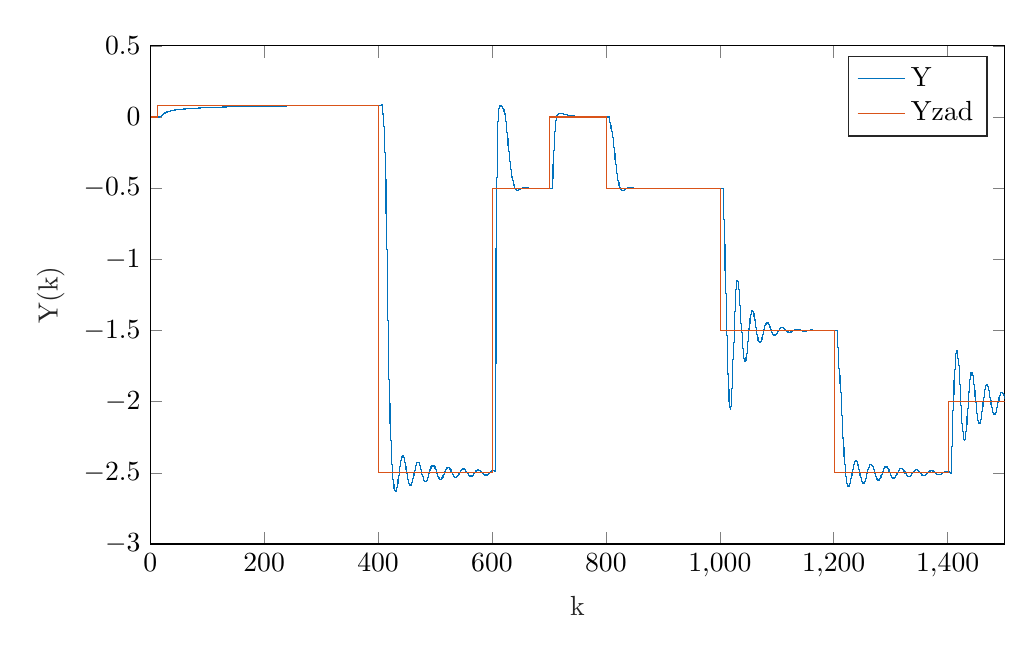
\begin{tikzpicture}

\begin{axis}[%
width=4.272in,
height=2.491in,
at={(0.717in,0.423in)},
scale only axis,
xmin=0,
xmax=1500,
xlabel style={font=\color{white!15!black}},
xlabel={k},
ymin=-3,
ymax=0.5,
ylabel style={font=\color{white!15!black}},
ylabel={Y(k)},
axis background/.style={fill=white},
legend style={legend cell align=left, align=left, draw=white!15!black}
]
\addplot[const plot, color=mycolor1] table[row sep=crcr] {%
1	0\\
2	0\\
3	0\\
4	0\\
5	0\\
6	0\\
7	0\\
8	0\\
9	0\\
10	0\\
11	0\\
12	0\\
13	0\\
14	0\\
15	0\\
16	0\\
17	0.00154612562740659\\
18	0.00481302550632309\\
19	0.00850529760815839\\
20	0.0120426757160726\\
21	0.0152869851355684\\
22	0.0183273233860898\\
23	0.0212865722126942\\
24	0.0241538159726894\\
25	0.0268382889550922\\
26	0.0292628297677317\\
27	0.0314066638261541\\
28	0.0333016099931466\\
29	0.035000427238321\\
30	0.0365480016393794\\
31	0.0379708910364497\\
32	0.039281769206905\\
33	0.0404886623868421\\
34	0.0416009944208155\\
35	0.0426304162112579\\
36	0.0435887286429526\\
37	0.0444858233480385\\
38	0.0453290568449552\\
39	0.0461245071872559\\
40	0.0468764360509503\\
41	0.0475867038109741\\
42	0.0482574633565301\\
43	0.0488914933273054\\
44	0.0494918912315548\\
45	0.0500617474830508\\
46	0.0506039539691616\\
47	0.0511211357160887\\
48	0.0516156434163398\\
49	0.0520895687303708\\
50	0.0525447665667211\\
51	0.0529828790477498\\
52	0.0534053593331134\\
53	0.0538134943149614\\
54	0.0542084254955921\\
55	0.0545911676535089\\
56	0.0549626251922956\\
57	0.0553236062770415\\
58	0.0556748349771517\\
59	0.0560169616738054\\
60	0.05635057198554\\
61	0.0566761944401839\\
62	0.0569943070897611\\
63	0.0573053432340158\\
64	0.0576096963906165\\
65	0.0579077246266307\\
66	0.0581997543463486\\
67	0.05848608361449\\
68	0.0587669850807086\\
69	0.0590427085605818\\
70	0.059313483319502\\
71	0.0595795200986763\\
72	0.0598410129165025\\
73	0.0600981406736684\\
74	0.0603510685862261\\
75	0.0605999494674705\\
76	0.0608449248765756\\
77	0.0610861261495165\\
78	0.0613236753257528\\
79	0.0615576859824004\\
80	0.0617882639861303\\
81	0.0620155081717557\\
82	0.0622395109553725\\
83	0.0624603588889727\\
84	0.0626781331626344\\
85	0.0628929100596795\\
86	0.0631047613695807\\
87	0.0633137547628544\\
88	0.0635199541317134\\
89	0.0637234198998373\\
90	0.0639242093042593\\
91	0.0641223766520501\\
92	0.0643179735541969\\
93	0.0645110491388317\\
94	0.0647016502457377\\
95	0.0648898216038738\\
96	0.0650756059934789\\
97	0.0652590443941662\\
98	0.0654401761202791\\
99	0.0656190389446583\\
100	0.0657956692118574\\
101	0.0659701019417484\\
102	0.0661423709243681\\
103	0.0663125088067788\\
104	0.0664805471726422\\
105	0.0666465166151441\\
106	0.0668104468038486\\
107	0.0669723665460058\\
108	0.0671323038427939\\
109	0.067290285940929\\
110	0.0674463393800415\\
111	0.0676004900361794\\
112	0.0677527631617695\\
113	0.0679031834223366\\
114	0.0680517749302561\\
115	0.0681985612757907\\
116	0.0683435655556397\\
117	0.0684868103992114\\
118	0.0686283179928101\\
119	0.0687681101019106\\
120	0.0689062080916837\\
121	0.0690426329459162\\
122	0.0691774052844615\\
123	0.0693105453793417\\
124	0.0694420731696159\\
125	0.0695720082751151\\
126	0.0697003700091398\\
127	0.0698271773902055\\
128	0.0699524491529164\\
129	0.0700762037580378\\
130	0.0701984594018359\\
131	0.0703192340247445\\
132	0.0704385453194145\\
133	0.0705564107381978\\
134	0.0706728475001119\\
135	0.0707878725973294\\
136	0.0709015028012298\\
137	0.0710137546680518\\
138	0.0711246445441778\\
139	0.0712341885710819\\
140	0.0713424026899686\\
141	0.0714493026461279\\
142	0.0715549039930304\\
143	0.071659222096184\\
144	0.0717622721367711\\
145	0.0718640691150854\\
146	0.071964627853784\\
147	0.0720639630009701\\
148	0.0721620890331207\\
149	0.072259020257871\\
150	0.0723547708166688\\
151	0.0724493546873074\\
152	0.0725427856863487\\
153	0.0726350774714445\\
154	0.0727262435435641\\
155	0.0728162972491363\\
156	0.0729052517821124\\
157	0.0729931201859561\\
158	0.0730799153555665\\
159	0.0731656500391395\\
160	0.0732503368399719\\
161	0.0733339882182133\\
162	0.0734166164925693\\
163	0.0734982338419596\\
164	0.0735788523071348\\
165	0.0736584837922546\\
166	0.0737371400664302\\
167	0.0738148327652342\\
168	0.0738915733921784\\
169	0.0739673733201642\\
170	0.0740422437929054\\
171	0.0741161959263262\\
172	0.0741892407099357\\
173	0.0742613890081807\\
174	0.0743326515617775\\
175	0.0744030389890242\\
176	0.0744725617870951\\
177	0.0745412303333172\\
178	0.0746090548864304\\
179	0.0746760455878323\\
180	0.074742212462808\\
181	0.074807565421745\\
182	0.0748721142613355\\
183	0.0749358686657648\\
184	0.0749988382078878\\
185	0.0750610323503925\\
186	0.0751224604469528\\
187	0.0751831317433688\\
188	0.0752430553786971\\
189	0.0753022403863698\\
190	0.0753606956953032\\
191	0.075418430130996\\
192	0.0754754524166182\\
193	0.0755317711740892\\
194	0.0755873949251473\\
195	0.075642332092409\\
196	0.0756965910004191\\
197	0.075750179876692\\
198	0.0758031068527437\\
199	0.0758553799651145\\
200	0.0759070071563835\\
201	0.0759579962761738\\
202	0.0760083550821489\\
203	0.0760580912410013\\
204	0.0761072123294317\\
205	0.0761557258351199\\
206	0.0762036391576875\\
207	0.0762509596096518\\
208	0.0762976944173723\\
209	0.0763438507219873\\
210	0.0763894355803437\\
211	0.0764344559659183\\
212	0.0764789187697301\\
213	0.0765228308012456\\
214	0.0765661987892749\\
215	0.0766090293828609\\
216	0.0766513291521597\\
217	0.0766931045893127\\
218	0.076734362109312\\
219	0.0767751080508566\\
220	0.0768153486772013\\
221	0.0768550901769975\\
222	0.0768943386651267\\
223	0.0769331001835256\\
224	0.0769713807020034\\
225	0.0770091861190522\\
226	0.0770465222626486\\
227	0.0770833948910487\\
228	0.0771198096935746\\
229	0.0771557722913938\\
230	0.077191288238291\\
231	0.0772263630214325\\
232	0.0772610020621226\\
233	0.0772952107165534\\
234	0.0773289942765464\\
235	0.0773623579702876\\
236	0.0773953069630541\\
237	0.0774278463579348\\
238	0.0774599811965432\\
239	0.0774917164597226\\
240	0.0775230570682449\\
241	0.0775540078835023\\
242	0.0775845737081912\\
243	0.07761475928699\\
244	0.0776445693072292\\
245	0.0776740083995552\\
246	0.0777030811385868\\
247	0.0777317920435652\\
248	0.077760145578997\\
249	0.0777881461552905\\
250	0.0778157981293854\\
251	0.0778431058053762\\
252	0.0778700734351283\\
253	0.077896705218888\\
254	0.0779230053058865\\
255	0.0779489777949362\\
256	0.0779746267350223\\
257	0.0779999561258862\\
258	0.0780249699186046\\
259	0.0780496720161606\\
260	0.0780740662740099\\
261	0.0780981565006402\\
262	0.0781219464581247\\
263	0.0781454398626698\\
264	0.0781686403851562\\
265	0.0781915516516751\\
266	0.0782141772440575\\
267	0.0782365207003983\\
268	0.0782585855155744\\
269	0.0782803751417574\\
270	0.07830189298892\\
271	0.0783231424253374\\
272	0.0783441267780829\\
273	0.078364849333518\\
274	0.078385313337777\\
275	0.0784055219972463\\
276	0.0784254784790382\\
277	0.0784451859114596\\
278	0.0784646473844749\\
279	0.0784838659501646\\
280	0.0785028446231782\\
281	0.0785215863811814\\
282	0.0785400941652997\\
283	0.0785583708805555\\
284	0.0785764193963012\\
285	0.0785942425466469\\
286	0.0786118431308837\\
287	0.0786292239139014\\
288	0.0786463876266023\\
289	0.0786633369663096\\
290	0.0786800745971718\\
291	0.0786966031505616\\
292	0.0787129252254709\\
293	0.0787290433889014\\
294	0.0787449601762495\\
295	0.0787606780916886\\
296	0.0787761996085453\\
297	0.0787915271696724\\
298	0.0788066631878169\\
299	0.0788216100459841\\
300	0.0788363700977974\\
301	0.0788509456678538\\
302	0.0788653390520754\\
303	0.0788795525180569\\
304	0.0788935883054088\\
305	0.0789074486260967\\
306	0.0789211356647768\\
307	0.0789346515791273\\
308	0.0789479985001757\\
309	0.0789611785326232\\
310	0.0789741937551639\\
311	0.0789870462208014\\
312	0.0789997379571614\\
313	0.0790122709668002\\
314	0.0790246472275097\\
315	0.0790368686926197\\
316	0.0790489372912952\\
317	0.0790608549288314\\
318	0.0790726234869444\\
319	0.0790842448240589\\
320	0.0790957207755926\\
321	0.0791070531542366\\
322	0.0791182437502333\\
323	0.0791292943316506\\
324	0.0791402066446525\\
325	0.0791509824137671\\
326	0.0791616233421512\\
327	0.0791721311118516\\
328	0.0791825073840636\\
329	0.0791927537993858\\
330	0.0792028719780727\\
331	0.0792128635202839\\
332	0.0792227300063298\\
333	0.0792324729969154\\
334	0.0792420940333806\\
335	0.0792515946379374\\
336	0.0792609763139045\\
337	0.0792702405459396\\
338	0.0792793888002681\\
339	0.0792884225249094\\
340	0.0792973431499007\\
341	0.0793061520875176\\
342	0.0793148507324926\\
343	0.0793234404622307\\
344	0.0793319226370223\\
345	0.0793402986002541\\
346	0.0793485696786162\\
347	0.0793567371823084\\
348	0.0793648024052427\\
349	0.079372766625244\\
350	0.079380631104248\\
351	0.0793883970884971\\
352	0.0793960658087336\\
353	0.0794036384803909\\
354	0.0794111163037819\\
355	0.0794185004642856\\
356	0.0794257921325312\\
357	0.0794329924645801\\
358	0.0794401026021056\\
359	0.0794471236725702\\
360	0.0794540567894016\\
361	0.079460903052165\\
362	0.0794676635467353\\
363	0.0794743393454656\\
364	0.0794809315073541\\
365	0.0794874410782096\\
366	0.0794938690908142\\
367	0.0795002165650841\\
368	0.0795064845082292\\
369	0.0795126739149097\\
370	0.0795187857673915\\
371	0.0795248210356998\\
372	0.0795307806777699\\
373	0.0795366656395974\\
374	0.0795424768553857\\
375	0.0795482152476919\\
376	0.0795538817275712\\
377	0.0795594771947192\\
378	0.0795650025376127\\
379	0.0795704586336484\\
380	0.0795758463492806\\
381	0.0795811665401564\\
382	0.0795864200512498\\
383	0.079591607716994\\
384	0.0795967303614122\\
385	0.0796017887982463\\
386	0.0796067838310848\\
387	0.0796117162534887\\
388	0.0796165868491154\\
389	0.0796213963918425\\
390	0.0796261456458879\\
391	0.079630835365931\\
392	0.0796354662972302\\
393	0.0796400391757401\\
394	0.0796445547282272\\
395	0.0796490136723836\\
396	0.0796534167169401\\
397	0.0796577645617774\\
398	0.0796620578980358\\
399	0.0796662974082241\\
400	0.0796704837663267\\
401	0.0796746176379095\\
402	0.0796786996802247\\
403	0.0796827305423139\\
404	0.0796867108651104\\
405	0.07969064128154\\
406	0.0845757958796227\\
407	0.0670027845084107\\
408	0.0210906253855427\\
409	-0.0236205706860865\\
410	-0.0655270993969085\\
411	-0.129721635151812\\
412	-0.251097531549191\\
413	-0.441414406184249\\
414	-0.678411218290466\\
415	-0.933793317244093\\
416	-1.18812461742177\\
417	-1.42875417856831\\
418	-1.64811366592854\\
419	-1.84234436583709\\
420	-2.01020988015783\\
421	-2.1522511999046\\
422	-2.27014345126923\\
423	-2.36621738525439\\
424	-2.44311304139391\\
425	-2.50353753223768\\
426	-2.54921119723929\\
427	-2.58350050691551\\
428	-2.6088906360494\\
429	-2.62591041528639\\
430	-2.63401727005398\\
431	-2.6323611217926\\
432	-2.62109354702012\\
433	-2.6017591543385\\
434	-2.57660839775368\\
435	-2.54789156932781\\
436	-2.51751303347774\\
437	-2.48707358469532\\
438	-2.45807586372896\\
439	-2.43202135934904\\
440	-2.41034241894028\\
441	-2.39424127035265\\
442	-2.38453509132338\\
443	-2.3815805841636\\
444	-2.3852878545691\\
445	-2.39518895034781\\
446	-2.41053038748006\\
447	-2.43030253410282\\
448	-2.45332476969449\\
449	-2.47791224447465\\
450	-2.50236386826525\\
451	-2.52547543062535\\
452	-2.54619204929826\\
453	-2.56351486389294\\
454	-2.5766284546149\\
455	-2.58499947887581\\
456	-2.58837446304052\\
457	-2.58674522449112\\
458	-2.58033387080907\\
459	-2.56959347203918\\
460	-2.55520448460071\\
461	-2.5380493374969\\
462	-2.51916129373761\\
463	-2.49965585067876\\
464	-2.48065657126092\\
465	-2.46322477650823\\
466	-2.44829830032145\\
467	-2.43664217975217\\
468	-2.4288115397883\\
469	-2.4251287056562\\
470	-2.42567491913\\
471	-2.43029601539366\\
472	-2.43862090099521\\
473	-2.45009053992209\\
474	-2.46399465419268\\
475	-2.47951418545863\\
476	-2.49576746355039\\
477	-2.51185726366487\\
478	-2.52691667777981\\
479	-2.54015241425116\\
480	-2.55088418681192\\
481	-2.55857868077187\\
482	-2.56287637304134\\
483	-2.5636094993538\\
484	-2.56080978456905\\
485	-2.55470508511852\\
486	-2.54570475026007\\
487	-2.53437423993838\\
488	-2.52140033610546\\
489	-2.5075490533913\\
490	-2.49361905152085\\
491	-2.48039380392898\\
492	-2.46859588910605\\
493	-2.4588465227997\\
494	-2.45163287204531\\
495	-2.4472848901314\\
496	-2.44596253711637\\
497	-2.44765342018976\\
498	-2.45218017927656\\
499	-2.45921642457829\\
500	-2.46830971420183\\
501	-2.47890990992657\\
502	-2.49040122115562\\
503	-2.50213629018469\\
504	-2.51347074523835\\
505	-2.52379672594796\\
506	-2.53257395923065\\
507	-2.53935703678375\\
508	-2.54381763536867\\
509	-2.54576055269442\\
510	-2.54513263100385\\
511	-2.54202392889373\\
512	-2.53666088758306\\
513	-2.52939170994755\\
514	-2.52066469678924\\
515	-2.51100081252367\\
516	-2.50096221650422\\
517	-2.49111883103684\\
518	-2.48201517091414\\
519	-2.4741396059957\\
520	-2.46789797502386\\
521	-2.46359305406527\\
522	-2.46141086758085\\
523	-2.4614142835125\\
524	-2.46354381943635\\
525	-2.46762515159467\\
526	-2.4733824874954\\
527	-2.48045673961908\\
528	-2.48842731032391\\
529	-2.49683624504222\\
530	-2.50521350928109\\
531	-2.51310217561255\\
532	-2.52008235790869\\
533	-2.52579279809461\\
534	-2.52994909974316\\
535	-2.53235772220005\\
536	-2.53292500975322\\
537	-2.53166074179091\\
538	-2.52867595520279\\
539	-2.52417510361914\\
540	-2.51844296266314\\
541	-2.5118270388566\\
542	-2.50471655726969\\
543	-2.49751935246564\\
544	-2.49063813660728\\
545	-2.48444764712655\\
546	-2.47927407961171\\
547	-2.47537800237038\\
548	-2.47294165499686\\
549	-2.47206119072136\\
550	-2.4727440697396\\
551	-2.47491148176537\\
552	-2.47840539500796\\
553	-2.4829996087111\\
554	-2.48841402989469\\
555	-2.49433129679819\\
556	-2.50041482225122\\
557	-2.50632731949419\\
558	-2.51174889241478\\
559	-2.51639381674421\\
560	-2.52002520722469\\
561	-2.52246685992209\\
562	-2.52361168206761\\
563	-2.52342627697414\\
564	-2.52195143903747\\
565	-2.51929852955257\\
566	-2.51564193847939\\
567	-2.51120807521901\\
568	-2.50626155341567\\
569	-2.50108941946349\\
570	-2.49598440200392\\
571	-2.49122821558393\\
572	-2.48707592909019\\
573	-2.48374231123806\\
574	-2.48139090289776\\
575	-2.48012635783258\\
576	-2.47999036148383\\
577	-2.4809612036402\\
578	-2.48295686383301\\
579	-2.48584128153151\\
580	-2.48943333421493\\
581	-2.49351793737668\\
582	-2.49785860974707\\
583	-2.50221081059755\\
584	-2.50633534948848\\
585	-2.51001118853899\\
586	-2.51304700088946\\
587	-2.5152909155364\\
588	-2.51663796805055\\
589	-2.51703488871338\\
590	-2.51648199309816\\
591	-2.51503209176043\\
592	-2.5127864993967\\
593	-2.50988839055938\\
594	-2.50651390732944\\
595	-2.50286156153393\\
596	-2.49914057785218\\
597	-2.49555888446646\\
598	-2.49231146873841\\
599	-2.4895697757506\\
600	-2.48747274176881\\
601	-2.48611993170132\\
602	-2.48556710158345\\
603	-2.48582434745104\\
604	-2.48685684358962\\
605	-2.48858802692465\\
606	-1.7324359664974\\
607	-0.925817589741942\\
608	-0.424779200541433\\
609	-0.159505550512516\\
610	-0.0289939132346655\\
611	0.0333243712734609\\
612	0.0626932106065012\\
613	0.0760311651334238\\
614	0.0807294588986423\\
615	0.0803587966968554\\
616	0.0771942371212164\\
617	0.0727102316054089\\
618	0.0676310185177029\\
619	0.0616204056874696\\
620	0.052797370781958\\
621	0.0392413902947632\\
622	0.0208685657812292\\
623	-0.00222270752565571\\
624	-0.0309857086043743\\
625	-0.0664577825341976\\
626	-0.108628740683056\\
627	-0.154193143724368\\
628	-0.198901039532898\\
629	-0.24009939782866\\
630	-0.277089269136635\\
631	-0.310359254490586\\
632	-0.340958102517753\\
633	-0.369752754001645\\
634	-0.396874215474308\\
635	-0.421829236177362\\
636	-0.443913892503552\\
637	-0.46262943543326\\
638	-0.477903398790632\\
639	-0.490020973825343\\
640	-0.499400900411082\\
641	-0.506402820351557\\
642	-0.511266752831311\\
643	-0.514174195672502\\
644	-0.515346520585989\\
645	-0.515098399391887\\
646	-0.513808239839831\\
647	-0.511879199914219\\
648	-0.509644878035255\\
649	-0.507337279241795\\
650	-0.505109045379587\\
651	-0.503065833464453\\
652	-0.501284929688362\\
653	-0.499821489212348\\
654	-0.498706381072759\\
655	-0.497941239145773\\
656	-0.497499296967791\\
657	-0.497332682359346\\
658	-0.497382963924127\\
659	-0.497591290664477\\
660	-0.497904930384155\\
661	-0.498279538347506\\
662	-0.498678627640296\\
663	-0.499072292261483\\
664	-0.499436606720569\\
665	-0.499753917443085\\
666	-0.500013411303166\\
667	-0.500210830275868\\
668	-0.500347750112957\\
669	-0.500429889504188\\
670	-0.500465208946511\\
671	-0.500462525435714\\
672	-0.500430738561392\\
673	-0.500378423869259\\
674	-0.500313554077599\\
675	-0.500243224312056\\
676	-0.500173364019355\\
677	-0.50010852763716\\
678	-0.500051837975171\\
679	-0.500005087335347\\
680	-0.499968952593393\\
681	-0.499943254334486\\
682	-0.499927201131048\\
683	-0.499919591661892\\
684	-0.49991897504954\\
685	-0.499923783252009\\
686	-0.499932446834632\\
687	-0.499943498052334\\
688	-0.499955648608022\\
689	-0.49996784150572\\
690	-0.499979271748657\\
691	-0.4999893784875\\
692	-0.499997819386381\\
693	-0.500004437600279\\
694	-0.500009227513081\\
695	-0.500012301338577\\
696	-0.500013856794221\\
697	-0.50001414584921\\
698	-0.500013445722862\\
699	-0.500012034039663\\
700	-0.500010169651567\\
701	-0.500008079680117\\
702	-0.500005952275992\\
703	-0.500003933935361\\
704	-0.500002130107097\\
705	-0.500000608061113\\
706	-0.434104575093478\\
707	-0.335143058921437\\
708	-0.238494550642786\\
709	-0.159026764634348\\
710	-0.0994896248675272\\
711	-0.0569716545269629\\
712	-0.0272737379813749\\
713	-0.00690676583844924\\
714	0.00666890558615057\\
715	0.0153257663129994\\
716	0.0204993862925761\\
717	0.0233063194378509\\
718	0.0245915052771797\\
719	0.0249522219572591\\
720	0.0247694114614413\\
721	0.0242577043411886\\
722	0.0235280112686928\\
723	0.0226446573118359\\
724	0.0216609839968767\\
725	0.0206294776834945\\
726	0.0195726183848028\\
727	0.0185300891924163\\
728	0.0175547934222242\\
729	0.0166355170468049\\
730	0.0157437096952002\\
731	0.014858676492528\\
732	0.0139777026372015\\
733	0.0131182014657107\\
734	0.0123013260384412\\
735	0.0115374994436553\\
736	0.0108231245770461\\
737	0.0101464372513385\\
738	0.00949700393494119\\
739	0.00887166242748833\\
740	0.00827404716903536\\
741	0.00770991381451585\\
742	0.00718238547404665\\
743	0.00669015678866449\\
744	0.00622895428898569\\
745	0.0057943858915834\\
746	0.00538424181446421\\
747	0.00499787255555407\\
748	0.00463555859435101\\
749	0.00429782137501412\\
750	0.00398400083298865\\
751	0.00369230851624742\\
752	0.00342051944616519\\
753	0.00316667600767545\\
754	0.00292957759227622\\
755	0.00270867080535067\\
756	0.00250357744222005\\
757	0.00231367086485207\\
758	0.00213793283581552\\
759	0.00197511850677131\\
760	0.00182404854787848\\
761	0.0016838093291821\\
762	0.00155376166050067\\
763	0.00143340311190943\\
764	0.00132220853079252\\
765	0.00121955382252055\\
766	0.00112474500261565\\
767	0.00103711354457953\\
768	0.000956082540327384\\
769	0.000881178782744762\\
770	0.000812005751889052\\
771	0.000748192139400644\\
772	0.000689358990823609\\
773	0.000635118649082627\\
774	0.000585093835067147\\
775	0.000538941035576572\\
776	0.000496361487269977\\
777	0.000457095358268289\\
778	0.000420906736298632\\
779	0.000387569957089322\\
780	0.000356864413933694\\
781	0.000328578034389358\\
782	0.000302514238292236\\
783	0.000278496551278174\\
784	0.000256368069530744\\
785	0.000235986891942892\\
786	0.000217220859893383\\
787	0.000199944422699811\\
788	0.000184038626231566\\
789	0.000169392816787449\\
790	0.000155906069679942\\
791	0.000143487264865944\\
792	0.000132053699012165\\
793	0.000121529159711427\\
794	0.000111842490080481\\
795	0.000102927055211853\\
796	9.47209194363137e-05\\
797	8.71671783309049e-05\\
798	8.02139620446374e-05\\
799	7.38139867422427e-05\\
800	6.79238502153199e-05\\
801	6.25033823293814e-05\\
802	5.7515257162099e-05\\
803	5.29248701693575e-05\\
804	4.87003348506445e-05\\
805	4.48124326254298e-05\\
806	-0.0120706204758309\\
807	-0.0373392912829335\\
808	-0.0628253753021901\\
809	-0.0835342690403782\\
810	-0.0996758084191743\\
811	-0.116937938198521\\
812	-0.141144401031242\\
813	-0.174246498730172\\
814	-0.214253443924899\\
815	-0.256781867510394\\
816	-0.297562676212949\\
817	-0.334281881283637\\
818	-0.366665790092678\\
819	-0.395432411436698\\
820	-0.421233190165819\\
821	-0.444209480988285\\
822	-0.464118757892093\\
823	-0.4806721507949\\
824	-0.493781692986169\\
825	-0.503614898204866\\
826	-0.510183232937327\\
827	-0.514202729692009\\
828	-0.516367544468262\\
829	-0.517068619877655\\
830	-0.516563522890544\\
831	-0.515037313251013\\
832	-0.51274316370392\\
833	-0.510027551626813\\
834	-0.507240874218656\\
835	-0.504653707617455\\
836	-0.502418617802623\\
837	-0.500586852292672\\
838	-0.499154009016599\\
839	-0.498098451353293\\
840	-0.497396666149687\\
841	-0.49702025254303\\
842	-0.496928316300671\\
843	-0.497065750407361\\
844	-0.497369140153749\\
845	-0.497775985808515\\
846	-0.498234251148571\\
847	-0.498698230139699\\
848	-0.49913535302816\\
849	-0.499525527394063\\
850	-0.499856471274111\\
851	-0.500121809625982\\
852	-0.500319252876325\\
853	-0.500450361806173\\
854	-0.50052087009731\\
855	-0.500539996729705\\
856	-0.500518948553795\\
857	-0.500469169784638\\
858	-0.500401007019555\\
859	-0.500323136759457\\
860	-0.500242576444682\\
861	-0.50016490128625\\
862	-0.500094388020173\\
863	-0.500034028699818\\
864	-0.499985519704189\\
865	-0.499949345101173\\
866	-0.499924977202649\\
867	-0.499911226627791\\
868	-0.499906465921593\\
869	-0.499908866988455\\
870	-0.499916596738428\\
871	-0.49992792478249\\
872	-0.499941299957575\\
873	-0.499955392586777\\
874	-0.499969118982202\\
875	-0.499981659761408\\
876	-0.499992462481157\\
877	-0.500001223966568\\
878	-0.500007853523854\\
879	-0.500012424566004\\
880	-0.500015125607888\\
881	-0.500016218186898\\
882	-0.500016003745978\\
883	-0.500014797669651\\
884	-0.500012907918804\\
885	-0.500010617253441\\
886	-0.500008169792034\\
887	-0.500005762409257\\
888	-0.500003542765657\\
889	-0.500001611210448\\
890	-0.500000025571156\\
891	-0.4999988078378\\
892	-0.49999795125337\\
893	-0.499997427434536\\
894	-0.499997193112034\\
895	-0.499997196208846\\
896	-0.499997381180599\\
897	-0.499997693464406\\
898	-0.499998082902958\\
899	-0.499998506081188\\
900	-0.499998927612348\\
901	-0.499999320532218\\
902	-0.499999666026319\\
903	-0.49999995271043\\
904	-0.500000175636132\\
905	-0.500000335138475\\
906	-0.500000435610525\\
907	-0.500000484286151\\
908	-0.500000490095419\\
909	-0.500000462674932\\
910	-0.500000411567751\\
911	-0.500000345621811\\
912	-0.500000272581457\\
913	-0.500000198846478\\
914	-0.500000129372425\\
915	-0.500000067685514\\
916	-0.500000015984738\\
917	-0.499999975306118\\
918	-0.499999945725285\\
919	-0.49999992657665\\
920	-0.499999916670641\\
921	-0.499999914494448\\
922	-0.499999918386359\\
923	-0.499999926678362\\
924	-0.499999937805488\\
925	-0.499999950383042\\
926	-0.499999963254488\\
927	-0.499999975513657\\
928	-0.499999986505651\\
929	-0.499999995810999\\
930	-0.500000003217989\\
931	-0.500000008687847\\
932	-0.500000012316776\\
933	-0.500000014298172\\
934	-0.500000014887409\\
935	-0.500000014370832\\
936	-0.500000013039953\\
937	-0.500000011171296\\
938	-0.500000009011887\\
939	-0.500000006770039\\
940	-0.500000004610817\\
941	-0.500000002655387\\
942	-0.500000000983382\\
943	-0.499999999637431\\
944	-0.499999998629017\\
945	-0.499999997945002\\
946	-0.499999997554213\\
947	-0.499999997413674\\
948	-0.499999997474152\\
949	-0.499999997684817\\
950	-0.49999999799693\\
951	-0.499999998366522\\
952	-0.499999998756147\\
953	-0.49999999913579\\
954	-0.499999999483087\\
955	-0.499999999782995\\
956	-0.500000000027059\\
957	-0.500000000212431\\
958	-0.500000000340743\\
959	-0.50000000041696\\
960	-0.500000000448276\\
961	-0.50000000044313\\
962	-0.500000000410361\\
963	-0.500000000358544\\
964	-0.500000000295494\\
965	-0.50000000022793\\
966	-0.500000000161302\\
967	-0.500000000099724\\
968	-0.500000000046023\\
969	-0.500000000001856\\
970	-0.499999999967871\\
971	-0.499999999943903\\
972	-0.499999999929175\\
973	-0.49999999992249\\
974	-0.499999999922406\\
975	-0.499999999927388\\
976	-0.499999999935931\\
977	-0.499999999946649\\
978	-0.499999999958336\\
979	-0.499999999970008\\
980	-0.499999999980907\\
981	-0.499999999990506\\
982	-0.499999999998483\\
983	-0.500000000004698\\
984	-0.500000000009158\\
985	-0.500000000011982\\
986	-0.500000000013368\\
987	-0.500000000013561\\
988	-0.500000000012826\\
989	-0.500000000011429\\
990	-0.500000000009614\\
991	-0.500000000007598\\
992	-0.500000000005557\\
993	-0.500000000003632\\
994	-0.500000000001919\\
995	-0.500000000000481\\
996	-0.499999999999347\\
997	-0.49999999999852\\
998	-0.499999999997983\\
999	-0.499999999997702\\
1000	-0.499999999997636\\
1001	-0.499999999997739\\
1002	-0.499999999997965\\
1003	-0.49999999999827\\
1004	-0.499999999998617\\
1005	-0.499999999998973\\
1006	-0.573098658675973\\
1007	-0.721356612948048\\
1008	-0.899152960682921\\
1009	-1.076614876777\\
1010	-1.23895623177571\\
1011	-1.38918994049307\\
1012	-1.53449480085931\\
1013	-1.67536598674278\\
1014	-1.80530632287564\\
1015	-1.91464062734424\\
1016	-1.99509445719519\\
1017	-2.04228273096484\\
1018	-2.05542943031351\\
1019	-2.03591200115136\\
1020	-1.98626027136733\\
1021	-1.91015174117555\\
1022	-1.81288891222419\\
1023	-1.70156780219019\\
1024	-1.58455971309329\\
1025	-1.47048348943893\\
1026	-1.36629806212097\\
1027	-1.27885745925072\\
1028	-1.21282881521447\\
1029	-1.17021012496288\\
1030	-1.15092015614724\\
1031	-1.15332265094527\\
1032	-1.17485405345536\\
1033	-1.2124376062036\\
1034	-1.26266848093919\\
1035	-1.32193002341324\\
1036	-1.38650582440908\\
1037	-1.45271800490319\\
1038	-1.51707577731565\\
1039	-1.57640220412664\\
1040	-1.627930401521\\
1041	-1.669381298794\\
1042	-1.69903980664781\\
1043	-1.71583448006072\\
1044	-1.71940892320725\\
1045	-1.7101640045409\\
1046	-1.68925648097683\\
1047	-1.65851557231982\\
1048	-1.62033241296652\\
1049	-1.57748318361179\\
1050	-1.53290716278677\\
1051	-1.48947661204882\\
1052	-1.44978227478779\\
1053	-1.41596303118819\\
1054	-1.38959438364821\\
1055	-1.37163844071728\\
1056	-1.3624503621219\\
1057	-1.36182961087656\\
1058	-1.36910160683999\\
1059	-1.38321558889971\\
1060	-1.40284683645002\\
1061	-1.42649516528745\\
1062	-1.45257551058885\\
1063	-1.47949943045065\\
1064	-1.50574797491894\\
1065	-1.5299366006017\\
1066	-1.55087213104169\\
1067	-1.5676010240424\\
1068	-1.57944683287849\\
1069	-1.5860351079504\\
1070	-1.58730348672246\\
1071	-1.58349505622552\\
1072	-1.57513412021148\\
1073	-1.56298474984764\\
1074	-1.54799423310826\\
1075	-1.53122530265045\\
1076	-1.51378247594874\\
1077	-1.4967386976163\\
1078	-1.48106845489453\\
1079	-1.46759261778041\\
1080	-1.45693862939526\\
1081	-1.44951769502211\\
1082	-1.44551869661058\\
1083	-1.44491701947489\\
1084	-1.4474954941078\\
1085	-1.45287424373978\\
1086	-1.46054628251561\\
1087	-1.4699160630824\\
1088	-1.48033866391532\\
1089	-1.49115778366988\\
1090	-1.50174111302073\\
1091	-1.51151193924093\\
1092	-1.51997602313932\\
1093	-1.52674291836615\\
1094	-1.53154102594759\\
1095	-1.53422584042\\
1096	-1.53478107916378\\
1097	-1.5333127043176\\
1098	-1.53003623708923\\
1099	-1.52525819529088\\
1100	-1.51935290690344\\
1101	-1.51273630621891\\
1102	-1.5058385474648\\
1103	-1.49907733196076\\
1104	-1.49283372303167\\
1105	-1.48743193309902\\
1106	-1.48312415228198\\
1107	-1.48008100784672\\
1108	-1.47838776333709\\
1109	-1.47804594079463\\
1110	-1.47897971637637\\
1111	-1.48104621520482\\
1112	-1.48404871227903\\
1113	-1.48775171604255\\
1114	-1.49189694667914\\
1115	-1.49621929923689\\
1116	-1.50046198363595\\
1117	-1.50439014745495\\
1118	-1.50780240756378\\
1119	-1.51053984250229\\
1120	-1.51249213078234\\
1121	-1.51360066279493\\
1122	-1.51385860547283\\
1123	-1.5133080557351\\
1124	-1.51203457381897\\
1125	-1.51015953064296\\
1126	-1.50783082246904\\
1127	-1.50521258982295\\
1128	-1.50247461687329\\
1129	-1.49978207759467\\
1130	-1.49728623683797\\
1131	-1.49511661423456\\
1132	-1.49337498757976\\
1133	-1.49213146368977\\
1134	-1.49142269306015\\
1135	-1.49125216293534\\
1136	-1.49159238166554\\
1137	-1.49238867182966\\
1138	-1.49356422319413\\
1139	-1.49502601871054\\
1140	-1.49667123482435\\
1141	-1.49839372760965\\
1142	-1.50009024459066\\
1143	-1.50166604474628\\
1144	-1.50303966280645\\
1145	-1.50414661570199\\
1146	-1.50494191636444\\
1147	-1.50540133044073\\
1148	-1.5055213821373\\
1149	-1.50531818327204\\
1150	-1.50482522136632\\
1151	-1.50409029487613\\
1152	-1.50317182333818\\
1153	-1.50213478484563\\
1154	-1.50104654142207\\
1155	-1.49997280434381\\
1156	-1.49897396741758\\
1157	-1.49810199905373\\
1158	-1.49739803705729\\
1159	-1.49689077735943\\
1160	-1.49659569354502\\
1161	-1.49651507184854\\
1162	-1.49663879953847\\
1163	-1.49694580573123\\
1164	-1.49740602422246\\
1165	-1.49798272860251\\
1166	-1.49863508071097\\
1167	-1.4993207337908\\
1168	-1.49999834053086\\
1169	-1.50062983227674\\
1170	-1.5011823576291\\
1171	-1.50162979492712\\
1172	-1.50195378218029\\
1173	-1.50214423828596\\
1174	-1.50219937928775\\
1175	-1.50212526147119\\
1176	-1.50193490784946\\
1177	-1.50164709483207\\
1178	-1.50128489062526\\
1179	-1.50087404554907\\
1180	-1.50044133672658\\
1181	-1.50001296567669\\
1182	-1.4996130977911\\
1183	-1.49926261842413\\
1184	-1.49897816255591\\
1185	-1.49877145505878\\
1186	-1.49864897789732\\
1187	-1.4986119604593\\
1188	-1.49865667082616\\
1189	-1.49877497010244\\
1190	-1.49895507962867\\
1191	-1.49918250242138\\
1192	-1.49944103567251\\
1193	-1.49971381051789\\
1194	-1.49998429826663\\
1195	-1.50023722842395\\
1196	-1.50045937257163\\
1197	-1.50064015883835\\
1198	-1.50077209359463\\
1199	-1.50085097942323\\
1200	-1.50087593064228\\
1201	-1.50084919903724\\
1202	-1.50077583240831\\
1203	-1.50066319658632\\
1204	-1.50052039736326\\
1205	-1.50035764212135\\
1206	-1.54245193535414\\
1207	-1.61894662023641\\
1208	-1.69978439417168\\
1209	-1.76821137260157\\
1210	-1.81968629459403\\
1211	-1.86880670001014\\
1212	-1.9335652868552\\
1213	-2.01181799616811\\
1214	-2.09520016026076\\
1215	-2.17766836946291\\
1216	-2.25531902071814\\
1217	-2.32584698892103\\
1218	-2.38810997992061\\
1219	-2.44178425737464\\
1220	-2.48709771505525\\
1221	-2.52462716672483\\
1222	-2.55478321463571\\
1223	-2.57720520094585\\
1224	-2.59148226369738\\
1225	-2.59782432453765\\
1226	-2.59630547591537\\
1227	-2.58853364423128\\
1228	-2.57610689352132\\
1229	-2.56001607379452\\
1230	-2.54105321834454\\
1231	-2.5200162075816\\
1232	-2.49799389889769\\
1233	-2.47636848904934\\
1234	-2.45656089374515\\
1235	-2.43978911857135\\
1236	-2.4269416844878\\
1237	-2.41857103697071\\
1238	-2.41493762626719\\
1239	-2.4160552218719\\
1240	-2.42171722188529\\
1241	-2.43150411879993\\
1242	-2.44479112549486\\
1243	-2.46077259273621\\
1244	-2.4785076830407\\
1245	-2.4969811291623\\
1246	-2.51517189707218\\
1247	-2.53209559726531\\
1248	-2.54686475849942\\
1249	-2.55873075449475\\
1250	-2.56711191461705\\
1251	-2.57162055638236\\
1252	-2.57208208735541\\
1253	-2.56854634525641\\
1254	-2.56128717836633\\
1255	-2.55078632463313\\
1256	-2.53770260071434\\
1257	-2.52282951593301\\
1258	-2.50704540976036\\
1259	-2.49125982501586\\
1260	-2.47635940689647\\
1261	-2.46315658736828\\
1262	-2.4523442413831\\
1263	-2.4444592247362\\
1264	-2.43985697867325\\
1265	-2.43869830036433\\
1266	-2.44094820505823\\
1267	-2.44638605039661\\
1268	-2.45462489802576\\
1269	-2.46513857419946\\
1270	-2.47729441215029\\
1271	-2.49038968791909\\
1272	-2.50369005679992\\
1273	-2.5164682917305\\
1274	-2.5280417440062\\
1275	-2.53780700378802\\
1276	-2.54527025695201\\
1277	-2.55007192239375\\
1278	-2.55200429416321\\
1279	-2.55102113401304\\
1280	-2.54723847709142\\
1281	-2.5409263397971\\
1282	-2.53249155678776\\
1283	-2.52245259054219\\
1284	-2.51140778809815\\
1285	-2.4999991194049\\
1286	-2.48887383198926\\
1287	-2.47864662839128\\
1288	-2.46986489348404\\
1289	-2.46297916477566\\
1290	-2.4583205269091\\
1291	-2.45608598489382\\
1292	-2.45633221924776\\
1293	-2.45897753206608\\
1294	-2.46381130488061\\
1295	-2.47050993470191\\
1296	-2.47865799221991\\
1297	-2.48777323444245\\
1298	-2.4973340737261\\
1299	-2.50680812575515\\
1300	-2.51568050667889\\
1301	-2.52348061065188\\
1302	-2.52980617081802\\
1303	-2.53434349651821\\
1304	-2.53688290090916\\
1305	-2.53732850227612\\
1306	-2.53570181254074\\
1307	-2.53213882377835\\
1308	-2.52688066224424\\
1309	-2.52025827988578\\
1310	-2.51267206195743\\
1311	-2.50456760296085\\
1312	-2.49640919543198\\
1313	-2.48865274695313\\
1314	-2.48171986501904\\
1315	-2.4759747225927\\
1316	-2.47170505702074\\
1317	-2.46910829734175\\
1318	-2.46828340625915\\
1319	-2.46922861059851\\
1320	-2.47184481803885\\
1321	-2.47594420559736\\
1322	-2.48126322947811\\
1323	-2.48747914621318\\
1324	-2.49422904216963\\
1325	-2.50113032873415\\
1326	-2.50780166009711\\
1327	-2.51388325904755\\
1328	-2.51905568799399\\
1329	-2.52305617709467\\
1330	-2.52569172250258\\
1331	-2.52684830092276\\
1332	-2.52649571702207\\
1333	-2.52468780957306\\
1334	-2.52155798679949\\
1335	-2.51731033036701\\
1336	-2.51220678274094\\
1337	-2.50655119044674\\
1338	-2.50067118988272\\
1339	-2.49489906840307\\
1340	-2.48955279353153\\
1341	-2.48491836960724\\
1342	-2.48123455796426\\
1343	-2.47868079909917\\
1344	-2.47736892658425\\
1345	-2.47733898996644\\
1346	-2.4785592339603\\
1347	-2.48093003562418\\
1348	-2.48429139465505\\
1349	-2.48843341169915\\
1350	-2.49310907641198\\
1351	-2.49804861716947\\
1352	-2.50297463191776\\
1353	-2.50761721865906\\
1354	-2.51172834992345\\
1355	-2.51509478579218\\
1356	-2.51754889414717\\
1357	-2.51897684561182\\
1358	-2.51932377495727\\
1359	-2.51859565006487\\
1360	-2.51685776070475\\
1361	-2.51422992570311\\
1362	-2.51087870803855\\
1363	-2.5070071093654\\
1364	-2.50284237304354\\
1365	-2.49862264302318\\
1366	-2.49458329278418\\
1367	-2.49094374681932\\
1368	-2.48789556605962\\
1369	-2.48559246390167\\
1370	-2.48414277244413\\
1371	-2.48360470419051\\
1372	-2.48398456913401\\
1373	-2.48523792606201\\
1374	-2.4872734825077\\
1375	-2.48995941859833\\
1376	-2.49313170071063\\
1377	-2.49660387257308\\
1378	-2.50017776312735\\
1379	-2.50365452972727\\
1380	-2.50684545952994\\
1381	-2.50958197905443\\
1382	-2.5117243703469\\
1383	-2.5131687610034\\
1384	-2.51385204350931\\
1385	-2.51375448539348\\
1386	-2.51289991273161\\
1387	-2.51135348095568\\
1388	-2.50921718215379\\
1389	-2.50662336876013\\
1390	-2.50372669036115\\
1391	-2.50069493390368\\
1392	-2.4976993197727\\
1393	-2.49490483138319\\
1394	-2.49246114188331\\
1395	-2.49049464988434\\
1396	-2.48910205201051\\
1397	-2.48834577151834\\
1398	-2.48825143894752\\
1399	-2.48880749275589\\
1400	-2.48996684433397\\
1401	-2.4916504401518\\
1402	-2.49375245936889\\
1403	-2.49614681117709\\
1404	-2.49869454373589\\
1405	-2.50125174574734\\
1406	-2.43417083863512\\
1407	-2.31700255693708\\
1408	-2.18577741944485\\
1409	-2.06022630445205\\
1410	-1.94883212620992\\
1411	-1.8527172281602\\
1412	-1.77184245189124\\
1413	-1.70782537686375\\
1414	-1.66326667474903\\
1415	-1.64020038930117\\
1416	-1.63904822253002\\
1417	-1.65847349750317\\
1418	-1.69582605028688\\
1419	-1.74771917309939\\
1420	-1.81046179828874\\
1421	-1.88027738528675\\
1422	-1.9533804366452\\
1423	-2.02601989843886\\
1424	-2.094560060527\\
1425	-2.15561156430522\\
1426	-2.20653857137805\\
1427	-2.24464074442773\\
1428	-2.26786715362922\\
1429	-2.27522945190111\\
1430	-2.26673854670309\\
1431	-2.24335073727491\\
1432	-2.20683449452304\\
1433	-2.15967402020769\\
1434	-2.10497502474689\\
1435	-2.04628985687519\\
1436	-1.98735644821152\\
1437	-1.9317923417749\\
1438	-1.88280734724984\\
1439	-1.84298469330804\\
1440	-1.81415050609651\\
1441	-1.79732780108789\\
1442	-1.79275883884441\\
1443	-1.79997634033944\\
1444	-1.81790550971574\\
1445	-1.84498203167524\\
1446	-1.87927282427783\\
1447	-1.9186037563384\\
1448	-1.96066765950271\\
1449	-2.00312981006176\\
1450	-2.04373119009882\\
1451	-2.08038451721\\
1452	-2.11126426711343\\
1453	-2.1348879310446\\
1454	-2.15018612875878\\
1455	-2.15655824416889\\
1456	-2.15390808391596\\
1457	-2.14265352953961\\
1458	-2.12370500703934\\
1459	-2.09841007784193\\
1460	-2.0684652084612\\
1461	-2.03580007732096\\
1462	-2.00244388798845\\
1463	-1.97038616420043\\
1464	-1.94144555967713\\
1465	-1.91715891882899\\
1466	-1.89869946618629\\
1467	-1.88682835360146\\
1468	-1.88187952603918\\
1469	-1.88377385402566\\
1470	-1.89205657633461\\
1471	-1.90595145658087\\
1472	-1.92442545443235\\
1473	-1.94625888806305\\
1474	-1.97011736764701\\
1475	-1.99462293032844\\
1476	-2.01842259373669\\
1477	-2.0402528882627\\
1478	-2.05899891105402\\
1479	-2.0737462014358\\
1480	-2.08382342559787\\
1481	-2.08883362846782\\
1482	-2.08867179257856\\
1483	-2.08352674715451\\
1484	-2.07386617144734\\
1485	-2.06040454931254\\
1486	-2.04405537967596\\
1487	-2.02587054550023\\
1488	-2.00697121417277\\
1489	-1.98847569169322\\
1490	-1.9714300261993\\
1491	-1.95674675907485\\
1492	-1.94515612820009\\
1493	-1.93717246730239\\
1494	-1.93307683339926\\
1495	-1.93291533189374\\
1496	-1.9365114117538\\
1497	-1.94348966606528\\
1498	-1.95330837585061\\
1499	-1.9652980778347\\
1500	-1.97870368526943\\
};
\addlegendentry{Y}

\addplot[const plot, color=mycolor2] table[row sep=crcr] {%
1	0\\
2	0\\
3	0\\
4	0\\
5	0\\
6	0\\
7	0\\
8	0\\
9	0\\
10	0\\
11	0\\
12	0.08\\
13	0.08\\
14	0.08\\
15	0.08\\
16	0.08\\
17	0.08\\
18	0.08\\
19	0.08\\
20	0.08\\
21	0.08\\
22	0.08\\
23	0.08\\
24	0.08\\
25	0.08\\
26	0.08\\
27	0.08\\
28	0.08\\
29	0.08\\
30	0.08\\
31	0.08\\
32	0.08\\
33	0.08\\
34	0.08\\
35	0.08\\
36	0.08\\
37	0.08\\
38	0.08\\
39	0.08\\
40	0.08\\
41	0.08\\
42	0.08\\
43	0.08\\
44	0.08\\
45	0.08\\
46	0.08\\
47	0.08\\
48	0.08\\
49	0.08\\
50	0.08\\
51	0.08\\
52	0.08\\
53	0.08\\
54	0.08\\
55	0.08\\
56	0.08\\
57	0.08\\
58	0.08\\
59	0.08\\
60	0.08\\
61	0.08\\
62	0.08\\
63	0.08\\
64	0.08\\
65	0.08\\
66	0.08\\
67	0.08\\
68	0.08\\
69	0.08\\
70	0.08\\
71	0.08\\
72	0.08\\
73	0.08\\
74	0.08\\
75	0.08\\
76	0.08\\
77	0.08\\
78	0.08\\
79	0.08\\
80	0.08\\
81	0.08\\
82	0.08\\
83	0.08\\
84	0.08\\
85	0.08\\
86	0.08\\
87	0.08\\
88	0.08\\
89	0.08\\
90	0.08\\
91	0.08\\
92	0.08\\
93	0.08\\
94	0.08\\
95	0.08\\
96	0.08\\
97	0.08\\
98	0.08\\
99	0.08\\
100	0.08\\
101	0.08\\
102	0.08\\
103	0.08\\
104	0.08\\
105	0.08\\
106	0.08\\
107	0.08\\
108	0.08\\
109	0.08\\
110	0.08\\
111	0.08\\
112	0.08\\
113	0.08\\
114	0.08\\
115	0.08\\
116	0.08\\
117	0.08\\
118	0.08\\
119	0.08\\
120	0.08\\
121	0.08\\
122	0.08\\
123	0.08\\
124	0.08\\
125	0.08\\
126	0.08\\
127	0.08\\
128	0.08\\
129	0.08\\
130	0.08\\
131	0.08\\
132	0.08\\
133	0.08\\
134	0.08\\
135	0.08\\
136	0.08\\
137	0.08\\
138	0.08\\
139	0.08\\
140	0.08\\
141	0.08\\
142	0.08\\
143	0.08\\
144	0.08\\
145	0.08\\
146	0.08\\
147	0.08\\
148	0.08\\
149	0.08\\
150	0.08\\
151	0.08\\
152	0.08\\
153	0.08\\
154	0.08\\
155	0.08\\
156	0.08\\
157	0.08\\
158	0.08\\
159	0.08\\
160	0.08\\
161	0.08\\
162	0.08\\
163	0.08\\
164	0.08\\
165	0.08\\
166	0.08\\
167	0.08\\
168	0.08\\
169	0.08\\
170	0.08\\
171	0.08\\
172	0.08\\
173	0.08\\
174	0.08\\
175	0.08\\
176	0.08\\
177	0.08\\
178	0.08\\
179	0.08\\
180	0.08\\
181	0.08\\
182	0.08\\
183	0.08\\
184	0.08\\
185	0.08\\
186	0.08\\
187	0.08\\
188	0.08\\
189	0.08\\
190	0.08\\
191	0.08\\
192	0.08\\
193	0.08\\
194	0.08\\
195	0.08\\
196	0.08\\
197	0.08\\
198	0.08\\
199	0.08\\
200	0.08\\
201	0.08\\
202	0.08\\
203	0.08\\
204	0.08\\
205	0.08\\
206	0.08\\
207	0.08\\
208	0.08\\
209	0.08\\
210	0.08\\
211	0.08\\
212	0.08\\
213	0.08\\
214	0.08\\
215	0.08\\
216	0.08\\
217	0.08\\
218	0.08\\
219	0.08\\
220	0.08\\
221	0.08\\
222	0.08\\
223	0.08\\
224	0.08\\
225	0.08\\
226	0.08\\
227	0.08\\
228	0.08\\
229	0.08\\
230	0.08\\
231	0.08\\
232	0.08\\
233	0.08\\
234	0.08\\
235	0.08\\
236	0.08\\
237	0.08\\
238	0.08\\
239	0.08\\
240	0.08\\
241	0.08\\
242	0.08\\
243	0.08\\
244	0.08\\
245	0.08\\
246	0.08\\
247	0.08\\
248	0.08\\
249	0.08\\
250	0.08\\
251	0.08\\
252	0.08\\
253	0.08\\
254	0.08\\
255	0.08\\
256	0.08\\
257	0.08\\
258	0.08\\
259	0.08\\
260	0.08\\
261	0.08\\
262	0.08\\
263	0.08\\
264	0.08\\
265	0.08\\
266	0.08\\
267	0.08\\
268	0.08\\
269	0.08\\
270	0.08\\
271	0.08\\
272	0.08\\
273	0.08\\
274	0.08\\
275	0.08\\
276	0.08\\
277	0.08\\
278	0.08\\
279	0.08\\
280	0.08\\
281	0.08\\
282	0.08\\
283	0.08\\
284	0.08\\
285	0.08\\
286	0.08\\
287	0.08\\
288	0.08\\
289	0.08\\
290	0.08\\
291	0.08\\
292	0.08\\
293	0.08\\
294	0.08\\
295	0.08\\
296	0.08\\
297	0.08\\
298	0.08\\
299	0.08\\
300	0.08\\
301	0.08\\
302	0.08\\
303	0.08\\
304	0.08\\
305	0.08\\
306	0.08\\
307	0.08\\
308	0.08\\
309	0.08\\
310	0.08\\
311	0.08\\
312	0.08\\
313	0.08\\
314	0.08\\
315	0.08\\
316	0.08\\
317	0.08\\
318	0.08\\
319	0.08\\
320	0.08\\
321	0.08\\
322	0.08\\
323	0.08\\
324	0.08\\
325	0.08\\
326	0.08\\
327	0.08\\
328	0.08\\
329	0.08\\
330	0.08\\
331	0.08\\
332	0.08\\
333	0.08\\
334	0.08\\
335	0.08\\
336	0.08\\
337	0.08\\
338	0.08\\
339	0.08\\
340	0.08\\
341	0.08\\
342	0.08\\
343	0.08\\
344	0.08\\
345	0.08\\
346	0.08\\
347	0.08\\
348	0.08\\
349	0.08\\
350	0.08\\
351	0.08\\
352	0.08\\
353	0.08\\
354	0.08\\
355	0.08\\
356	0.08\\
357	0.08\\
358	0.08\\
359	0.08\\
360	0.08\\
361	0.08\\
362	0.08\\
363	0.08\\
364	0.08\\
365	0.08\\
366	0.08\\
367	0.08\\
368	0.08\\
369	0.08\\
370	0.08\\
371	0.08\\
372	0.08\\
373	0.08\\
374	0.08\\
375	0.08\\
376	0.08\\
377	0.08\\
378	0.08\\
379	0.08\\
380	0.08\\
381	0.08\\
382	0.08\\
383	0.08\\
384	0.08\\
385	0.08\\
386	0.08\\
387	0.08\\
388	0.08\\
389	0.08\\
390	0.08\\
391	0.08\\
392	0.08\\
393	0.08\\
394	0.08\\
395	0.08\\
396	0.08\\
397	0.08\\
398	0.08\\
399	0.08\\
400	0.08\\
401	-2.5\\
402	-2.5\\
403	-2.5\\
404	-2.5\\
405	-2.5\\
406	-2.5\\
407	-2.5\\
408	-2.5\\
409	-2.5\\
410	-2.5\\
411	-2.5\\
412	-2.5\\
413	-2.5\\
414	-2.5\\
415	-2.5\\
416	-2.5\\
417	-2.5\\
418	-2.5\\
419	-2.5\\
420	-2.5\\
421	-2.5\\
422	-2.5\\
423	-2.5\\
424	-2.5\\
425	-2.5\\
426	-2.5\\
427	-2.5\\
428	-2.5\\
429	-2.5\\
430	-2.5\\
431	-2.5\\
432	-2.5\\
433	-2.5\\
434	-2.5\\
435	-2.5\\
436	-2.5\\
437	-2.5\\
438	-2.5\\
439	-2.5\\
440	-2.5\\
441	-2.5\\
442	-2.5\\
443	-2.5\\
444	-2.5\\
445	-2.5\\
446	-2.5\\
447	-2.5\\
448	-2.5\\
449	-2.5\\
450	-2.5\\
451	-2.5\\
452	-2.5\\
453	-2.5\\
454	-2.5\\
455	-2.5\\
456	-2.5\\
457	-2.5\\
458	-2.5\\
459	-2.5\\
460	-2.5\\
461	-2.5\\
462	-2.5\\
463	-2.5\\
464	-2.5\\
465	-2.5\\
466	-2.5\\
467	-2.5\\
468	-2.5\\
469	-2.5\\
470	-2.5\\
471	-2.5\\
472	-2.5\\
473	-2.5\\
474	-2.5\\
475	-2.5\\
476	-2.5\\
477	-2.5\\
478	-2.5\\
479	-2.5\\
480	-2.5\\
481	-2.5\\
482	-2.5\\
483	-2.5\\
484	-2.5\\
485	-2.5\\
486	-2.5\\
487	-2.5\\
488	-2.5\\
489	-2.5\\
490	-2.5\\
491	-2.5\\
492	-2.5\\
493	-2.5\\
494	-2.5\\
495	-2.5\\
496	-2.5\\
497	-2.5\\
498	-2.5\\
499	-2.5\\
500	-2.5\\
501	-2.5\\
502	-2.5\\
503	-2.5\\
504	-2.5\\
505	-2.5\\
506	-2.5\\
507	-2.5\\
508	-2.5\\
509	-2.5\\
510	-2.5\\
511	-2.5\\
512	-2.5\\
513	-2.5\\
514	-2.5\\
515	-2.5\\
516	-2.5\\
517	-2.5\\
518	-2.5\\
519	-2.5\\
520	-2.5\\
521	-2.5\\
522	-2.5\\
523	-2.5\\
524	-2.5\\
525	-2.5\\
526	-2.5\\
527	-2.5\\
528	-2.5\\
529	-2.5\\
530	-2.5\\
531	-2.5\\
532	-2.5\\
533	-2.5\\
534	-2.5\\
535	-2.5\\
536	-2.5\\
537	-2.5\\
538	-2.5\\
539	-2.5\\
540	-2.5\\
541	-2.5\\
542	-2.5\\
543	-2.5\\
544	-2.5\\
545	-2.5\\
546	-2.5\\
547	-2.5\\
548	-2.5\\
549	-2.5\\
550	-2.5\\
551	-2.5\\
552	-2.5\\
553	-2.5\\
554	-2.5\\
555	-2.5\\
556	-2.5\\
557	-2.5\\
558	-2.5\\
559	-2.5\\
560	-2.5\\
561	-2.5\\
562	-2.5\\
563	-2.5\\
564	-2.5\\
565	-2.5\\
566	-2.5\\
567	-2.5\\
568	-2.5\\
569	-2.5\\
570	-2.5\\
571	-2.5\\
572	-2.5\\
573	-2.5\\
574	-2.5\\
575	-2.5\\
576	-2.5\\
577	-2.5\\
578	-2.5\\
579	-2.5\\
580	-2.5\\
581	-2.5\\
582	-2.5\\
583	-2.5\\
584	-2.5\\
585	-2.5\\
586	-2.5\\
587	-2.5\\
588	-2.5\\
589	-2.5\\
590	-2.5\\
591	-2.5\\
592	-2.5\\
593	-2.5\\
594	-2.5\\
595	-2.5\\
596	-2.5\\
597	-2.5\\
598	-2.5\\
599	-2.5\\
600	-2.5\\
601	-0.5\\
602	-0.5\\
603	-0.5\\
604	-0.5\\
605	-0.5\\
606	-0.5\\
607	-0.5\\
608	-0.5\\
609	-0.5\\
610	-0.5\\
611	-0.5\\
612	-0.5\\
613	-0.5\\
614	-0.5\\
615	-0.5\\
616	-0.5\\
617	-0.5\\
618	-0.5\\
619	-0.5\\
620	-0.5\\
621	-0.5\\
622	-0.5\\
623	-0.5\\
624	-0.5\\
625	-0.5\\
626	-0.5\\
627	-0.5\\
628	-0.5\\
629	-0.5\\
630	-0.5\\
631	-0.5\\
632	-0.5\\
633	-0.5\\
634	-0.5\\
635	-0.5\\
636	-0.5\\
637	-0.5\\
638	-0.5\\
639	-0.5\\
640	-0.5\\
641	-0.5\\
642	-0.5\\
643	-0.5\\
644	-0.5\\
645	-0.5\\
646	-0.5\\
647	-0.5\\
648	-0.5\\
649	-0.5\\
650	-0.5\\
651	-0.5\\
652	-0.5\\
653	-0.5\\
654	-0.5\\
655	-0.5\\
656	-0.5\\
657	-0.5\\
658	-0.5\\
659	-0.5\\
660	-0.5\\
661	-0.5\\
662	-0.5\\
663	-0.5\\
664	-0.5\\
665	-0.5\\
666	-0.5\\
667	-0.5\\
668	-0.5\\
669	-0.5\\
670	-0.5\\
671	-0.5\\
672	-0.5\\
673	-0.5\\
674	-0.5\\
675	-0.5\\
676	-0.5\\
677	-0.5\\
678	-0.5\\
679	-0.5\\
680	-0.5\\
681	-0.5\\
682	-0.5\\
683	-0.5\\
684	-0.5\\
685	-0.5\\
686	-0.5\\
687	-0.5\\
688	-0.5\\
689	-0.5\\
690	-0.5\\
691	-0.5\\
692	-0.5\\
693	-0.5\\
694	-0.5\\
695	-0.5\\
696	-0.5\\
697	-0.5\\
698	-0.5\\
699	-0.5\\
700	-0.5\\
701	0\\
702	0\\
703	0\\
704	0\\
705	0\\
706	0\\
707	0\\
708	0\\
709	0\\
710	0\\
711	0\\
712	0\\
713	0\\
714	0\\
715	0\\
716	0\\
717	0\\
718	0\\
719	0\\
720	0\\
721	0\\
722	0\\
723	0\\
724	0\\
725	0\\
726	0\\
727	0\\
728	0\\
729	0\\
730	0\\
731	0\\
732	0\\
733	0\\
734	0\\
735	0\\
736	0\\
737	0\\
738	0\\
739	0\\
740	0\\
741	0\\
742	0\\
743	0\\
744	0\\
745	0\\
746	0\\
747	0\\
748	0\\
749	0\\
750	0\\
751	0\\
752	0\\
753	0\\
754	0\\
755	0\\
756	0\\
757	0\\
758	0\\
759	0\\
760	0\\
761	0\\
762	0\\
763	0\\
764	0\\
765	0\\
766	0\\
767	0\\
768	0\\
769	0\\
770	0\\
771	0\\
772	0\\
773	0\\
774	0\\
775	0\\
776	0\\
777	0\\
778	0\\
779	0\\
780	0\\
781	0\\
782	0\\
783	0\\
784	0\\
785	0\\
786	0\\
787	0\\
788	0\\
789	0\\
790	0\\
791	0\\
792	0\\
793	0\\
794	0\\
795	0\\
796	0\\
797	0\\
798	0\\
799	0\\
800	0\\
801	-0.5\\
802	-0.5\\
803	-0.5\\
804	-0.5\\
805	-0.5\\
806	-0.5\\
807	-0.5\\
808	-0.5\\
809	-0.5\\
810	-0.5\\
811	-0.5\\
812	-0.5\\
813	-0.5\\
814	-0.5\\
815	-0.5\\
816	-0.5\\
817	-0.5\\
818	-0.5\\
819	-0.5\\
820	-0.5\\
821	-0.5\\
822	-0.5\\
823	-0.5\\
824	-0.5\\
825	-0.5\\
826	-0.5\\
827	-0.5\\
828	-0.5\\
829	-0.5\\
830	-0.5\\
831	-0.5\\
832	-0.5\\
833	-0.5\\
834	-0.5\\
835	-0.5\\
836	-0.5\\
837	-0.5\\
838	-0.5\\
839	-0.5\\
840	-0.5\\
841	-0.5\\
842	-0.5\\
843	-0.5\\
844	-0.5\\
845	-0.5\\
846	-0.5\\
847	-0.5\\
848	-0.5\\
849	-0.5\\
850	-0.5\\
851	-0.5\\
852	-0.5\\
853	-0.5\\
854	-0.5\\
855	-0.5\\
856	-0.5\\
857	-0.5\\
858	-0.5\\
859	-0.5\\
860	-0.5\\
861	-0.5\\
862	-0.5\\
863	-0.5\\
864	-0.5\\
865	-0.5\\
866	-0.5\\
867	-0.5\\
868	-0.5\\
869	-0.5\\
870	-0.5\\
871	-0.5\\
872	-0.5\\
873	-0.5\\
874	-0.5\\
875	-0.5\\
876	-0.5\\
877	-0.5\\
878	-0.5\\
879	-0.5\\
880	-0.5\\
881	-0.5\\
882	-0.5\\
883	-0.5\\
884	-0.5\\
885	-0.5\\
886	-0.5\\
887	-0.5\\
888	-0.5\\
889	-0.5\\
890	-0.5\\
891	-0.5\\
892	-0.5\\
893	-0.5\\
894	-0.5\\
895	-0.5\\
896	-0.5\\
897	-0.5\\
898	-0.5\\
899	-0.5\\
900	-0.5\\
901	-0.5\\
902	-0.5\\
903	-0.5\\
904	-0.5\\
905	-0.5\\
906	-0.5\\
907	-0.5\\
908	-0.5\\
909	-0.5\\
910	-0.5\\
911	-0.5\\
912	-0.5\\
913	-0.5\\
914	-0.5\\
915	-0.5\\
916	-0.5\\
917	-0.5\\
918	-0.5\\
919	-0.5\\
920	-0.5\\
921	-0.5\\
922	-0.5\\
923	-0.5\\
924	-0.5\\
925	-0.5\\
926	-0.5\\
927	-0.5\\
928	-0.5\\
929	-0.5\\
930	-0.5\\
931	-0.5\\
932	-0.5\\
933	-0.5\\
934	-0.5\\
935	-0.5\\
936	-0.5\\
937	-0.5\\
938	-0.5\\
939	-0.5\\
940	-0.5\\
941	-0.5\\
942	-0.5\\
943	-0.5\\
944	-0.5\\
945	-0.5\\
946	-0.5\\
947	-0.5\\
948	-0.5\\
949	-0.5\\
950	-0.5\\
951	-0.5\\
952	-0.5\\
953	-0.5\\
954	-0.5\\
955	-0.5\\
956	-0.5\\
957	-0.5\\
958	-0.5\\
959	-0.5\\
960	-0.5\\
961	-0.5\\
962	-0.5\\
963	-0.5\\
964	-0.5\\
965	-0.5\\
966	-0.5\\
967	-0.5\\
968	-0.5\\
969	-0.5\\
970	-0.5\\
971	-0.5\\
972	-0.5\\
973	-0.5\\
974	-0.5\\
975	-0.5\\
976	-0.5\\
977	-0.5\\
978	-0.5\\
979	-0.5\\
980	-0.5\\
981	-0.5\\
982	-0.5\\
983	-0.5\\
984	-0.5\\
985	-0.5\\
986	-0.5\\
987	-0.5\\
988	-0.5\\
989	-0.5\\
990	-0.5\\
991	-0.5\\
992	-0.5\\
993	-0.5\\
994	-0.5\\
995	-0.5\\
996	-0.5\\
997	-0.5\\
998	-0.5\\
999	-0.5\\
1000	-0.5\\
1001	-1.5\\
1002	-1.5\\
1003	-1.5\\
1004	-1.5\\
1005	-1.5\\
1006	-1.5\\
1007	-1.5\\
1008	-1.5\\
1009	-1.5\\
1010	-1.5\\
1011	-1.5\\
1012	-1.5\\
1013	-1.5\\
1014	-1.5\\
1015	-1.5\\
1016	-1.5\\
1017	-1.5\\
1018	-1.5\\
1019	-1.5\\
1020	-1.5\\
1021	-1.5\\
1022	-1.5\\
1023	-1.5\\
1024	-1.5\\
1025	-1.5\\
1026	-1.5\\
1027	-1.5\\
1028	-1.5\\
1029	-1.5\\
1030	-1.5\\
1031	-1.5\\
1032	-1.5\\
1033	-1.5\\
1034	-1.5\\
1035	-1.5\\
1036	-1.5\\
1037	-1.5\\
1038	-1.5\\
1039	-1.5\\
1040	-1.5\\
1041	-1.5\\
1042	-1.5\\
1043	-1.5\\
1044	-1.5\\
1045	-1.5\\
1046	-1.5\\
1047	-1.5\\
1048	-1.5\\
1049	-1.5\\
1050	-1.5\\
1051	-1.5\\
1052	-1.5\\
1053	-1.5\\
1054	-1.5\\
1055	-1.5\\
1056	-1.5\\
1057	-1.5\\
1058	-1.5\\
1059	-1.5\\
1060	-1.5\\
1061	-1.5\\
1062	-1.5\\
1063	-1.5\\
1064	-1.5\\
1065	-1.5\\
1066	-1.5\\
1067	-1.5\\
1068	-1.5\\
1069	-1.5\\
1070	-1.5\\
1071	-1.5\\
1072	-1.5\\
1073	-1.5\\
1074	-1.5\\
1075	-1.5\\
1076	-1.5\\
1077	-1.5\\
1078	-1.5\\
1079	-1.5\\
1080	-1.5\\
1081	-1.5\\
1082	-1.5\\
1083	-1.5\\
1084	-1.5\\
1085	-1.5\\
1086	-1.5\\
1087	-1.5\\
1088	-1.5\\
1089	-1.5\\
1090	-1.5\\
1091	-1.5\\
1092	-1.5\\
1093	-1.5\\
1094	-1.5\\
1095	-1.5\\
1096	-1.5\\
1097	-1.5\\
1098	-1.5\\
1099	-1.5\\
1100	-1.5\\
1101	-1.5\\
1102	-1.5\\
1103	-1.5\\
1104	-1.5\\
1105	-1.5\\
1106	-1.5\\
1107	-1.5\\
1108	-1.5\\
1109	-1.5\\
1110	-1.5\\
1111	-1.5\\
1112	-1.5\\
1113	-1.5\\
1114	-1.5\\
1115	-1.5\\
1116	-1.5\\
1117	-1.5\\
1118	-1.5\\
1119	-1.5\\
1120	-1.5\\
1121	-1.5\\
1122	-1.5\\
1123	-1.5\\
1124	-1.5\\
1125	-1.5\\
1126	-1.5\\
1127	-1.5\\
1128	-1.5\\
1129	-1.5\\
1130	-1.5\\
1131	-1.5\\
1132	-1.5\\
1133	-1.5\\
1134	-1.5\\
1135	-1.5\\
1136	-1.5\\
1137	-1.5\\
1138	-1.5\\
1139	-1.5\\
1140	-1.5\\
1141	-1.5\\
1142	-1.5\\
1143	-1.5\\
1144	-1.5\\
1145	-1.5\\
1146	-1.5\\
1147	-1.5\\
1148	-1.5\\
1149	-1.5\\
1150	-1.5\\
1151	-1.5\\
1152	-1.5\\
1153	-1.5\\
1154	-1.5\\
1155	-1.5\\
1156	-1.5\\
1157	-1.5\\
1158	-1.5\\
1159	-1.5\\
1160	-1.5\\
1161	-1.5\\
1162	-1.5\\
1163	-1.5\\
1164	-1.5\\
1165	-1.5\\
1166	-1.5\\
1167	-1.5\\
1168	-1.5\\
1169	-1.5\\
1170	-1.5\\
1171	-1.5\\
1172	-1.5\\
1173	-1.5\\
1174	-1.5\\
1175	-1.5\\
1176	-1.5\\
1177	-1.5\\
1178	-1.5\\
1179	-1.5\\
1180	-1.5\\
1181	-1.5\\
1182	-1.5\\
1183	-1.5\\
1184	-1.5\\
1185	-1.5\\
1186	-1.5\\
1187	-1.5\\
1188	-1.5\\
1189	-1.5\\
1190	-1.5\\
1191	-1.5\\
1192	-1.5\\
1193	-1.5\\
1194	-1.5\\
1195	-1.5\\
1196	-1.5\\
1197	-1.5\\
1198	-1.5\\
1199	-1.5\\
1200	-1.5\\
1201	-2.5\\
1202	-2.5\\
1203	-2.5\\
1204	-2.5\\
1205	-2.5\\
1206	-2.5\\
1207	-2.5\\
1208	-2.5\\
1209	-2.5\\
1210	-2.5\\
1211	-2.5\\
1212	-2.5\\
1213	-2.5\\
1214	-2.5\\
1215	-2.5\\
1216	-2.5\\
1217	-2.5\\
1218	-2.5\\
1219	-2.5\\
1220	-2.5\\
1221	-2.5\\
1222	-2.5\\
1223	-2.5\\
1224	-2.5\\
1225	-2.5\\
1226	-2.5\\
1227	-2.5\\
1228	-2.5\\
1229	-2.5\\
1230	-2.5\\
1231	-2.5\\
1232	-2.5\\
1233	-2.5\\
1234	-2.5\\
1235	-2.5\\
1236	-2.5\\
1237	-2.5\\
1238	-2.5\\
1239	-2.5\\
1240	-2.5\\
1241	-2.5\\
1242	-2.5\\
1243	-2.5\\
1244	-2.5\\
1245	-2.5\\
1246	-2.5\\
1247	-2.5\\
1248	-2.5\\
1249	-2.5\\
1250	-2.5\\
1251	-2.5\\
1252	-2.5\\
1253	-2.5\\
1254	-2.5\\
1255	-2.5\\
1256	-2.5\\
1257	-2.5\\
1258	-2.5\\
1259	-2.5\\
1260	-2.5\\
1261	-2.5\\
1262	-2.5\\
1263	-2.5\\
1264	-2.5\\
1265	-2.5\\
1266	-2.5\\
1267	-2.5\\
1268	-2.5\\
1269	-2.5\\
1270	-2.5\\
1271	-2.5\\
1272	-2.5\\
1273	-2.5\\
1274	-2.5\\
1275	-2.5\\
1276	-2.5\\
1277	-2.5\\
1278	-2.5\\
1279	-2.5\\
1280	-2.5\\
1281	-2.5\\
1282	-2.5\\
1283	-2.5\\
1284	-2.5\\
1285	-2.5\\
1286	-2.5\\
1287	-2.5\\
1288	-2.5\\
1289	-2.5\\
1290	-2.5\\
1291	-2.5\\
1292	-2.5\\
1293	-2.5\\
1294	-2.5\\
1295	-2.5\\
1296	-2.5\\
1297	-2.5\\
1298	-2.5\\
1299	-2.5\\
1300	-2.5\\
1301	-2.5\\
1302	-2.5\\
1303	-2.5\\
1304	-2.5\\
1305	-2.5\\
1306	-2.5\\
1307	-2.5\\
1308	-2.5\\
1309	-2.5\\
1310	-2.5\\
1311	-2.5\\
1312	-2.5\\
1313	-2.5\\
1314	-2.5\\
1315	-2.5\\
1316	-2.5\\
1317	-2.5\\
1318	-2.5\\
1319	-2.5\\
1320	-2.5\\
1321	-2.5\\
1322	-2.5\\
1323	-2.5\\
1324	-2.5\\
1325	-2.5\\
1326	-2.5\\
1327	-2.5\\
1328	-2.5\\
1329	-2.5\\
1330	-2.5\\
1331	-2.5\\
1332	-2.5\\
1333	-2.5\\
1334	-2.5\\
1335	-2.5\\
1336	-2.5\\
1337	-2.5\\
1338	-2.5\\
1339	-2.5\\
1340	-2.5\\
1341	-2.5\\
1342	-2.5\\
1343	-2.5\\
1344	-2.5\\
1345	-2.5\\
1346	-2.5\\
1347	-2.5\\
1348	-2.5\\
1349	-2.5\\
1350	-2.5\\
1351	-2.5\\
1352	-2.5\\
1353	-2.5\\
1354	-2.5\\
1355	-2.5\\
1356	-2.5\\
1357	-2.5\\
1358	-2.5\\
1359	-2.5\\
1360	-2.5\\
1361	-2.5\\
1362	-2.5\\
1363	-2.5\\
1364	-2.5\\
1365	-2.5\\
1366	-2.5\\
1367	-2.5\\
1368	-2.5\\
1369	-2.5\\
1370	-2.5\\
1371	-2.5\\
1372	-2.5\\
1373	-2.5\\
1374	-2.5\\
1375	-2.5\\
1376	-2.5\\
1377	-2.5\\
1378	-2.5\\
1379	-2.5\\
1380	-2.5\\
1381	-2.5\\
1382	-2.5\\
1383	-2.5\\
1384	-2.5\\
1385	-2.5\\
1386	-2.5\\
1387	-2.5\\
1388	-2.5\\
1389	-2.5\\
1390	-2.5\\
1391	-2.5\\
1392	-2.5\\
1393	-2.5\\
1394	-2.5\\
1395	-2.5\\
1396	-2.5\\
1397	-2.5\\
1398	-2.5\\
1399	-2.5\\
1400	-2.5\\
1401	-2\\
1402	-2\\
1403	-2\\
1404	-2\\
1405	-2\\
1406	-2\\
1407	-2\\
1408	-2\\
1409	-2\\
1410	-2\\
1411	-2\\
1412	-2\\
1413	-2\\
1414	-2\\
1415	-2\\
1416	-2\\
1417	-2\\
1418	-2\\
1419	-2\\
1420	-2\\
1421	-2\\
1422	-2\\
1423	-2\\
1424	-2\\
1425	-2\\
1426	-2\\
1427	-2\\
1428	-2\\
1429	-2\\
1430	-2\\
1431	-2\\
1432	-2\\
1433	-2\\
1434	-2\\
1435	-2\\
1436	-2\\
1437	-2\\
1438	-2\\
1439	-2\\
1440	-2\\
1441	-2\\
1442	-2\\
1443	-2\\
1444	-2\\
1445	-2\\
1446	-2\\
1447	-2\\
1448	-2\\
1449	-2\\
1450	-2\\
1451	-2\\
1452	-2\\
1453	-2\\
1454	-2\\
1455	-2\\
1456	-2\\
1457	-2\\
1458	-2\\
1459	-2\\
1460	-2\\
1461	-2\\
1462	-2\\
1463	-2\\
1464	-2\\
1465	-2\\
1466	-2\\
1467	-2\\
1468	-2\\
1469	-2\\
1470	-2\\
1471	-2\\
1472	-2\\
1473	-2\\
1474	-2\\
1475	-2\\
1476	-2\\
1477	-2\\
1478	-2\\
1479	-2\\
1480	-2\\
1481	-2\\
1482	-2\\
1483	-2\\
1484	-2\\
1485	-2\\
1486	-2\\
1487	-2\\
1488	-2\\
1489	-2\\
1490	-2\\
1491	-2\\
1492	-2\\
1493	-2\\
1494	-2\\
1495	-2\\
1496	-2\\
1497	-2\\
1498	-2\\
1499	-2\\
1500	-2\\
};
\addlegendentry{Yzad}

\end{axis}
\end{tikzpicture}%
\caption{Regulacja rozmyta DMC, 2 regulatory}
\end{figure}

\begin{figure}[H]
\centering
% This file was created by matlab2tikz.
%
%The latest updates can be retrieved from
%  http://www.mathworks.com/matlabcentral/fileexchange/22022-matlab2tikz-matlab2tikz
%where you can also make suggestions and rate matlab2tikz.
%
\definecolor{mycolor1}{rgb}{0.00000,0.44700,0.74100}%
%
\begin{tikzpicture}

\begin{axis}[%
width=4.272in,
height=2.491in,
at={(0.717in,0.423in)},
scale only axis,
xmin=0,
xmax=1500,
xlabel style={font=\color{white!15!black}},
xlabel={k},
ymin=-1.1,
ymax=1.1,
ylabel style={font=\color{white!15!black}},
ylabel={U(k)},
axis background/.style={fill=white}
]
\addplot[const plot, color=mycolor1, forget plot] table[row sep=crcr] {%
1	0\\
2	0\\
3	0\\
4	0\\
5	0\\
6	0\\
7	0\\
8	0\\
9	0\\
10	0\\
11	0\\
12	0.0330701279452073\\
13	0.0421390407020668\\
14	0.0508822760567819\\
15	0.0608231162631033\\
16	0.0716857865990427\\
17	0.0852974046489884\\
18	0.099422522301179\\
19	0.112588731087575\\
20	0.124541532184824\\
21	0.135539099749561\\
22	0.146138296975326\\
23	0.156691283191389\\
24	0.167216474792391\\
25	0.177562342189596\\
26	0.187587787021186\\
27	0.197261408552741\\
28	0.206645095341199\\
29	0.215822494394517\\
30	0.224846449732113\\
31	0.23373054491556\\
32	0.242460568505628\\
33	0.251059067108251\\
34	0.259508110416807\\
35	0.267734701094451\\
36	0.275753888566238\\
37	0.283578602928934\\
38	0.291220220033835\\
39	0.298688841632775\\
40	0.305993712245249\\
41	0.313143773581277\\
42	0.320147565894535\\
43	0.327013052716209\\
44	0.333747525752629\\
45	0.340357594006983\\
46	0.34684922452665\\
47	0.353227804428787\\
48	0.359498206483357\\
49	0.365664850478212\\
50	0.371731757900503\\
51	0.377702599712854\\
52	0.383580737774535\\
53	0.389369260656463\\
54	0.395071014604013\\
55	0.400688630344034\\
56	0.406224546353216\\
57	0.411681029120146\\
58	0.417060190851785\\
59	0.422364005001923\\
60	0.427594319936384\\
61	0.43275287099748\\
62	0.437841291187121\\
63	0.442861120652958\\
64	0.447813815133138\\
65	0.452700753491711\\
66	0.457523244457231\\
67	0.462282532660953\\
68	0.466979804057573\\
69	0.471616190800125\\
70	0.476192775631145\\
71	0.480710595844133\\
72	0.485170646862459\\
73	0.489573885477006\\
74	0.493921232778793\\
75	0.498213576818495\\
76	0.50245177502101\\
77	0.506636656380009\\
78	0.510769023454549\\
79	0.514849654187379\\
80	0.518879303562422\\
81	0.522858705117025\\
82	0.526788572322899\\
83	0.530669599848227\\
84	0.53450246471211\\
85	0.538287827341402\\
86	0.542026332538937\\
87	0.54571861037129\\
88	0.54936527698338\\
89	0.552966935346537\\
90	0.556524175945987\\
91	0.560037577413165\\
92	0.56350770710774\\
93	0.566935121653778\\
94	0.570320367434059\\
95	0.573663981046196\\
96	0.57696648972386\\
97	0.580228411726127\\
98	0.583450256697673\\
99	0.586632526002321\\
100	0.589775713032192\\
101	0.592880303494544\\
102	0.595946775678166\\
103	0.598975600701051\\
104	0.601967242740926\\
105	0.604922159250051\\
106	0.607840801155607\\
107	0.610723613046866\\
108	0.613571033350225\\
109	0.616383494493113\\
110	0.619161423057674\\
111	0.621905239925066\\
112	0.624615360411135\\
113	0.627292194394167\\
114	0.629936146435347\\
115	0.63254761589253\\
116	0.635126997027837\\
117	0.637674679109582\\
118	0.640191046508976\\
119	0.642676478792019\\
120	0.645131350806957\\
121	0.647556032767648\\
122	0.649950890333163\\
123	0.652316284683901\\
124	0.654652572594492\\
125	0.656960106503728\\
126	0.659239234581746\\
127	0.661490300794678\\
128	0.663713644966936\\
129	0.665909602841325\\
130	0.668078506137132\\
131	0.670220682606337\\
132	0.672336456088079\\
133	0.674426146561499\\
134	0.676490070197081\\
135	0.678528539406573\\
136	0.680541862891605\\
137	0.682530345691075\\
138	0.684494289227389\\
139	0.686433991351626\\
140	0.688349746387692\\
141	0.690241845175534\\
142	0.692110575113452\\
143	0.693956220199582\\
144	0.695779061072581\\
145	0.697579375051562\\
146	0.699357436175326\\
147	0.701113515240912\\
148	0.702847879841521\\
149	0.704560794403814\\
150	0.706252520224648\\
151	0.707923315507245\\
152	0.709573435396836\\
153	0.711203132015797\\
154	0.712812654498295\\
155	0.714402249024467\\
156	0.715972158854142\\
157	0.71752262436013\\
158	0.719053883061089\\
159	0.720566169653978\\
160	0.722059716046122\\
161	0.723534751386882\\
162	0.724991502098955\\
163	0.726430191909313\\
164	0.727851041879778\\
165	0.729254270437251\\
166	0.730640093403607\\
167	0.732008724025251\\
168	0.733360373002347\\
169	0.734695248517735\\
170	0.736013556265523\\
171	0.737315499479378\\
172	0.738601278960514\\
173	0.739871093105372\\
174	0.741125137933018\\
175	0.74236360711224\\
176	0.743586691988367\\
177	0.7447945816098\\
178	0.745987462754269\\
179	0.74716551995481\\
180	0.748328935525471\\
181	0.749477889586755\\
182	0.750612560090788\\
183	0.751733122846229\\
184	0.752839751542919\\
185	0.753932617776272\\
186	0.755011891071414\\
187	0.756077738907059\\
188	0.75713032673915\\
189	0.758169818024239\\
190	0.759196374242631\\
191	0.760210154921276\\
192	0.761211317656428\\
193	0.762200018136062\\
194	0.76317641016205\\
195	0.764140645672109\\
196	0.765092874761515\\
197	0.766033245704579\\
198	0.766961904975909\\
199	0.767878997271429\\
200	0.768784665529183\\
201	0.769679050949919\\
202	0.770562293017442\\
203	0.771434529518754\\
204	0.772295896563982\\
205	0.773146528606079\\
206	0.773986558460325\\
207	0.774816117323603\\
208	0.775635334793478\\
209	0.776444338887062\\
210	0.777243256059671\\
211	0.778032211223285\\
212	0.778811327764799\\
213	0.779580727564079\\
214	0.780340531011812\\
215	0.781090857027171\\
216	0.781831823075271\\
217	0.782563545184443\\
218	0.783286137963312\\
219	0.783999714617682\\
220	0.78470438696724\\
221	0.785400265462069\\
222	0.786087459198976\\
223	0.786766075937642\\
224	0.787436222116585\\
225	0.788098002868948\\
226	0.788751522038107\\
227	0.789396882193104\\
228	0.790034184643904\\
229	0.790663529456485\\
230	0.791285015467749\\
231	0.79189874030027\\
232	0.792504800376871\\
233	0.793103290935037\\
234	0.793694306041162\\
235	0.794277938604637\\
236	0.79485428039177\\
237	0.795423422039554\\
238	0.795985453069273\\
239	0.796540461899953\\
240	0.797088535861656\\
241	0.797629761208626\\
242	0.79816422313228\\
243	0.798692005774044\\
244	0.799213192238054\\
245	0.799727864603698\\
246	0.800236103938014\\
247	0.800737990307952\\
248	0.801233602792484\\
249	0.801723019494582\\
250	0.802206317553046\\
251	0.802683573154206\\
252	0.803154861543478\\
253	0.803620257036788\\
254	0.804079833031867\\
255	0.804533662019405\\
256	0.804981815594083\\
257	0.805424364465468\\
258	0.805861378468787\\
259	0.806292926575567\\
260	0.806719076904158\\
261	0.807139896730125\\
262	0.807555452496521\\
263	0.807965809824038\\
264	0.808371033521041\\
265	0.808771187593475\\
266	0.809166335254665\\
267	0.809556538934993\\
268	0.809941860291467\\
269	0.810322360217165\\
270	0.810698098850579\\
271	0.811069135584844\\
272	0.811435529076853\\
273	0.811797337256269\\
274	0.812154617334427\\
275	0.812507425813131\\
276	0.812855818493345\\
277	0.813199850483782\\
278	0.813539576209389\\
279	0.813875049419729\\
280	0.814206323197269\\
281	0.81453344996556\\
282	0.814856481497327\\
283	0.815175468922458\\
284	0.815490462735896\\
285	0.81580151280544\\
286	0.816108668379452\\
287	0.816411978094466\\
288	0.816711489982712\\
289	0.817007251479549\\
290	0.817299309430803\\
291	0.817587710100021\\
292	0.817872499175639\\
293	0.818153721778059\\
294	0.818431422466647\\
295	0.818705645246636\\
296	0.81897643357596\\
297	0.819243830371991\\
298	0.819507878018206\\
299	0.819768618370767\\
300	0.820026092765024\\
301	0.820280342021936\\
302	0.820531406454419\\
303	0.820779325873615\\
304	0.821024139595084\\
305	0.821265886444919\\
306	0.821504604765795\\
307	0.821740332422934\\
308	0.821973106810006\\
309	0.822202964854952\\
310	0.822429943025741\\
311	0.822654077336056\\
312	0.822875403350909\\
313	0.823093956192185\\
314	0.823309770544129\\
315	0.823522880658754\\
316	0.823733320361192\\
317	0.823941123054972\\
318	0.824146321727242\\
319	0.82434894895392\\
320	0.824549036904788\\
321	0.82474661734852\\
322	0.824941721657646\\
323	0.825134380813466\\
324	0.825324625410893\\
325	0.82551248566324\\
326	0.82569799140695\\
327	0.82588117210627\\
328	0.826062056857861\\
329	0.826240674395358\\
330	0.826417053093873\\
331	0.826591220974438\\
332	0.826763205708403\\
333	0.826933034621769\\
334	0.827100734699474\\
335	0.827266332589631\\
336	0.827429854607701\\
337	0.82759132674063\\
338	0.82775077465092\\
339	0.827908223680664\\
340	0.828063698855525\\
341	0.82821722488866\\
342	0.828368826184611\\
343	0.82851852684313\\
344	0.828666350662974\\
345	0.828812321145642\\
346	0.828956461499069\\
347	0.829098794641276\\
348	0.829239343203975\\
349	0.829378129536129\\
350	0.829515175707464\\
351	0.829650503511949\\
352	0.829784134471216\\
353	0.829916089837959\\
354	0.830046390599269\\
355	0.830175057479948\\
356	0.830302110945766\\
357	0.830427571206686\\
358	0.830551458220052\\
359	0.830673791693729\\
360	0.830794591089208\\
361	0.83091387562468\\
362	0.831031664278056\\
363	0.831147975789969\\
364	0.83126282866672\\
365	0.831376241183203\\
366	0.831488231385785\\
367	0.831598817095153\\
368	0.831708015909126\\
369	0.831815845205433\\
370	0.831922322144452\\
371	0.832027463671923\\
372	0.832131286521622\\
373	0.832233807217999\\
374	0.832335042078796\\
375	0.832435007217613\\
376	0.832533718546462\\
377	0.832631191778279\\
378	0.832727442429401\\
379	0.832822485822024\\
380	0.832916337086623\\
381	0.83300901116434\\
382	0.83310052280935\\
383	0.833190886591191\\
384	0.833280116897068\\
385	0.833368227934129\\
386	0.833455233731708\\
387	0.833541148143551\\
388	0.833625984849999\\
389	0.833709757360158\\
390	0.833792479014035\\
391	0.833874162984647\\
392	0.833954822280108\\
393	0.834034469745686\\
394	0.834113118065836\\
395	0.83419077976621\\
396	0.834267467215637\\
397	0.834343192628085\\
398	0.83441796806459\\
399	0.83449180543517\\
400	0.834564716500712\\
401	0.215637943426111\\
402	-0.344886506048839\\
403	-0.175918107677354\\
404	-0.184534229394373\\
405	-0.228962940167582\\
406	-0.483348409382865\\
407	-0.819991852199803\\
408	-1\\
409	-1\\
410	-1\\
411	-1\\
412	-1\\
413	-1\\
414	-1\\
415	-1\\
416	-1\\
417	-1\\
418	-1\\
419	-1\\
420	-1\\
421	-0.995290442212849\\
422	-1\\
423	-1\\
424	-0.99346186298132\\
425	-0.982344666596961\\
426	-0.967989778138644\\
427	-0.955782989857372\\
428	-0.947600568655251\\
429	-0.94217672505365\\
430	-0.938209813395468\\
431	-0.934993317099465\\
432	-0.9328785770628\\
433	-0.932710362088032\\
434	-0.934993656702207\\
435	-0.939691347509707\\
436	-0.946310015609516\\
437	-0.954142055835758\\
438	-0.962532882350641\\
439	-0.97098577758562\\
440	-0.979132192415392\\
441	-0.98671324826291\\
442	-0.99319217382635\\
443	-0.998427080397803\\
444	-1\\
445	-1\\
446	-1\\
447	-0.998208133007871\\
448	-0.994747805245838\\
449	-0.990107240717532\\
450	-0.984764503820961\\
451	-0.978913280793043\\
452	-0.972735267019931\\
453	-0.966513870698263\\
454	-0.960609373275572\\
455	-0.95539747666495\\
456	-0.951197563263023\\
457	-0.948236097338694\\
458	-0.946643040224754\\
459	-0.94646200772268\\
460	-0.947660282538158\\
461	-0.950133922986986\\
462	-0.953714561860547\\
463	-0.958172077040894\\
464	-0.963234014058616\\
465	-0.968601408046907\\
466	-0.973967569911969\\
467	-0.979037403931197\\
468	-0.983542335376538\\
469	-0.98725202195241\\
470	-0.989987198033338\\
471	-0.991627774210027\\
472	-0.992113828433705\\
473	-0.991446519166614\\
474	-0.989687579514557\\
475	-0.986955943967591\\
476	-0.983421240784284\\
477	-0.979293979468652\\
478	-0.974813336977522\\
479	-0.970233606621953\\
480	-0.965810094997338\\
481	-0.961785077702815\\
482	-0.958374379069261\\
483	-0.955755374748812\\
484	-0.954057091932548\\
485	-0.953353361826116\\
486	-0.953659492312833\\
487	-0.954932703955328\\
488	-0.957076253041494\\
489	-0.95994679231839\\
490	-0.963364275264353\\
491	-0.967123637157716\\
492	-0.97100737639522\\
493	-0.974798130015601\\
494	-0.978290536532716\\
495	-0.981301820952079\\
496	-0.983680677736466\\
497	-0.985314163350674\\
498	-0.986132408631106\\
499	-0.986111050453964\\
500	-0.985271361032652\\
501	-0.983678124419574\\
502	-0.981435381929984\\
503	-0.978680243805455\\
504	-0.975575048642991\\
505	-0.972298235099532\\
506	-0.969034375516474\\
507	-0.965963891061777\\
508	-0.963253017700653\\
509	-0.961044612036656\\
510	-0.959450364989789\\
511	-0.958544923032001\\
512	-0.958362301120984\\
513	-0.958894812749373\\
514	-0.960094553708835\\
515	-0.961877280833411\\
516	-0.964128348659927\\
517	-0.966710228170272\\
518	-0.969471048208325\\
519	-0.97225357616454\\
520	-0.974904083780957\\
521	-0.97728061183859\\
522	-0.979260236185489\\
523	-0.980745031280421\\
524	-0.981666515860324\\
525	-0.981988444624129\\
526	-0.981707880844144\\
527	-0.980854550939428\\
528	-0.97948854648803\\
529	-0.977696503731575\\
530	-0.975586455297677\\
531	-0.973281611869933\\
532	-0.970913389728347\\
533	-0.968614049218895\\
534	-0.966509344143672\\
535	-0.964711597159745\\
536	-0.963313606256459\\
537	-0.962383748416646\\
538	-0.961962577580084\\
539	-0.962061117793435\\
540	-0.962660936039991\\
541	-0.963715953627392\\
542	-0.965155833420545\\
543	-0.966890675867539\\
544	-0.968816680308555\\
545	-0.970822385444178\\
546	-0.972795094465786\\
547	-0.974627111598773\\
548	-0.976221459833038\\
549	-0.977496805681421\\
550	-0.97839137838704\\
551	-0.978865732997269\\
552	-0.97890426664213\\
553	-0.97851545466384\\
554	-0.977730828362794\\
555	-0.976602769500896\\
556	-0.975201248203351\\
557	-0.973609679553725\\
558	-0.971920118165984\\
559	-0.970228046803566\\
560	-0.968627041656147\\
561	-0.967203609945876\\
562	-0.966032492140836\\
563	-0.965172699068937\\
564	-0.964664512993926\\
565	-0.964527622609736\\
566	-0.96476048861295\\
567	-0.965340954870138\\
568	-0.966228037570654\\
569	-0.967364748960436\\
570	-0.968681750279716\\
571	-0.970101585379688\\
572	-0.971543224444279\\
573	-0.97292664572693\\
574	-0.974177199344052\\
575	-0.97522952670219\\
576	-0.976030847543779\\
577	-0.976543469929156\\
578	-0.976746423832154\\
579	-0.976636164601441\\
580	-0.976226337325421\\
581	-0.975546636527215\\
582	-0.974640837011938\\
583	-0.973564110244619\\
584	-0.972379775135877\\
585	-0.971155660970785\\
586	-0.969960281588127\\
587	-0.968859031878965\\
588	-0.967910618482024\\
589	-0.967163924962263\\
590	-0.966655487353578\\
591	-0.966407719434604\\
592	-0.966427980482878\\
593	-0.96670852476191\\
594	-0.967227315855593\\
595	-0.96794963486425\\
596	-0.968830363937287\\
597	-0.969816789345913\\
598	-0.970851743689896\\
599	-0.971876895730974\\
600	-0.972835998126699\\
601	0.199984473688776\\
602	0.613684275296077\\
603	1\\
604	1\\
605	1\\
606	1\\
607	1\\
608	0.953970208101516\\
609	0.850389019414759\\
610	0.722877367997524\\
611	0.588038220411518\\
612	0.452706508113316\\
613	0.318935277497594\\
614	0.187051557527914\\
615	0.0690380170644404\\
616	-0.0147147735580368\\
617	-0.0764768926042413\\
618	-0.134499185332498\\
619	-0.195046230716664\\
620	-0.251222238794758\\
621	-0.299121020725665\\
622	-0.320831785573837\\
623	-0.333792611459532\\
624	-0.345165644093104\\
625	-0.358205564971455\\
626	-0.372147270328505\\
627	-0.387166148243214\\
628	-0.400921320811854\\
629	-0.411029831216859\\
630	-0.417402678744779\\
631	-0.420916193863069\\
632	-0.42296956268193\\
633	-0.424690171539703\\
634	-0.42634609920686\\
635	-0.427618379257591\\
636	-0.428092387187298\\
637	-0.427636861750725\\
638	-0.426499079253799\\
639	-0.425119049554666\\
640	-0.423873700969407\\
641	-0.422875088277638\\
642	-0.422235937471945\\
643	-0.421681659136638\\
644	-0.421145265329224\\
645	-0.420665265174594\\
646	-0.420311830881869\\
647	-0.420117837904375\\
648	-0.420085996709769\\
649	-0.420182724903943\\
650	-0.420350265581989\\
651	-0.420542116119811\\
652	-0.420730284531466\\
653	-0.420904718778755\\
654	-0.421066695827831\\
655	-0.421217645885524\\
656	-0.421354010079707\\
657	-0.42146827583214\\
658	-0.421553265474942\\
659	-0.421606320457181\\
660	-0.421630458759117\\
661	-0.421632812458096\\
662	-0.42161968331272\\
663	-0.421598275275733\\
664	-0.421571642799697\\
665	-0.421541303719569\\
666	-0.421508925835172\\
667	-0.421476769929955\\
668	-0.421447182509779\\
669	-0.421422043563215\\
670	-0.421402383409277\\
671	-0.421388255127141\\
672	-0.421379098337631\\
673	-0.421374111343658\\
674	-0.421372495911249\\
675	-0.421373569168534\\
676	-0.421376730186124\\
677	-0.421381392646627\\
678	-0.42138695756546\\
679	-0.421392840379778\\
680	-0.421398533850719\\
681	-0.42140366230631\\
682	-0.421408014143957\\
683	-0.421411489066904\\
684	-0.421414095849975\\
685	-0.421415890961829\\
686	-0.421416949920915\\
687	-0.4214173643172\\
688	-0.421417244118027\\
689	-0.421416714881988\\
690	-0.421415907663751\\
691	-0.421414946047623\\
692	-0.421413934041124\\
693	-0.421412951004844\\
694	-0.421412052639944\\
695	-0.421411274808235\\
696	-0.421410637939925\\
697	-0.421410150206582\\
698	-0.421409809463147\\
699	-0.42140960484106\\
700	-0.421409518664058\\
701	-0.127993931442108\\
702	-0.117153896137113\\
703	-0.110157781916283\\
704	-0.0909540287478854\\
705	-0.0597307677299965\\
706	-0.0185222826103598\\
707	0.0214919480168885\\
708	0.0522525473038701\\
709	0.0719655275476492\\
710	0.0824105487081709\\
711	0.0866951900180782\\
712	0.0875196954438125\\
713	0.0865247602455716\\
714	0.0844164821973779\\
715	0.0813849492240343\\
716	0.077544759239032\\
717	0.073159494562109\\
718	0.068608817822961\\
719	0.0642308655461252\\
720	0.0601920917734306\\
721	0.0557633577035103\\
722	0.0527706901412638\\
723	0.0497155081570926\\
724	0.0464879080203598\\
725	0.0432611098866416\\
726	0.0400525842274205\\
727	0.0371187781176305\\
728	0.0345480405969825\\
729	0.032255283765386\\
730	0.0301207944740966\\
731	0.0280462087649167\\
732	0.0260121983640275\\
733	0.0240656845029486\\
734	0.0222630825843853\\
735	0.020629151921883\\
736	0.0191467844824888\\
737	0.0177759320733844\\
738	0.0164819405881048\\
739	0.0152517871253028\\
740	0.0140919869813777\\
741	0.013020792024053\\
742	0.0120251638945708\\
743	0.0111177095082742\\
744	0.0102846895738166\\
745	0.0095098598698724\\
746	0.00878614618594939\\
747	0.00810822823646992\\
748	0.00747710642012929\\
749	0.00689512104708114\\
750	0.00636116645002004\\
751	0.00587101729020747\\
752	0.00541865674693036\\
753	0.00499871109611243\\
754	0.00460811168063297\\
755	0.00424581550722118\\
756	0.00391149067607562\\
757	0.00360421178742796\\
758	0.00332195347624925\\
759	0.00306200833597941\\
760	0.00282179365589994\\
761	0.00259939054918717\\
762	0.00239381669129709\\
763	0.00220413921353575\\
764	0.00202958954275002\\
765	0.00186913676451568\\
766	0.00172148414576811\\
767	0.00158539900720136\\
768	0.00145980892863411\\
769	0.00134388955406725\\
770	0.00123701912299735\\
771	0.00113863482132223\\
772	0.00104814519848965\\
773	0.000964909803211221\\
774	0.000888280991584544\\
775	0.000817669659036452\\
776	0.000752581640892184\\
777	0.00069261018365728\\
778	0.000637399402670992\\
779	0.000586606427892231\\
780	0.000539884646747468\\
781	0.000496891439791629\\
782	0.000457305795446492\\
783	0.000420847235575499\\
784	0.000387272002454171\\
785	0.000356365083052649\\
786	0.000327927395645616\\
787	0.000301766308695232\\
788	0.000277696482090619\\
789	0.00025554412677173\\
790	0.000235151486100846\\
791	0.000216378373769219\\
792	0.000199099454340461\\
793	0.000183199934247289\\
794	0.000168572120944045\\
795	0.000155114130303142\\
796	0.000142730577785373\\
797	0.000131333850092274\\
798	0.00012084465556792\\
799	0.000111191391351846\\
800	0.000102308710918685\\
801	-0.206558671737849\\
802	-0.19504140142797\\
803	-0.17874235967168\\
804	-0.179667772579339\\
805	-0.189461623644971\\
806	-0.236859974419828\\
807	-0.291202587400362\\
808	-0.334920018323711\\
809	-0.362118041818529\\
810	-0.374354628791709\\
811	-0.380348487759581\\
812	-0.387282984804113\\
813	-0.397054280724967\\
814	-0.407834524797463\\
815	-0.416972909058977\\
816	-0.423097156601526\\
817	-0.426402466702572\\
818	-0.427857492158448\\
819	-0.428378207137242\\
820	-0.428449249044595\\
821	-0.426312882873803\\
822	-0.427012589268435\\
823	-0.426939493447413\\
824	-0.425995084732986\\
825	-0.424667525575787\\
826	-0.422972646735273\\
827	-0.421624775596444\\
828	-0.420847124594614\\
829	-0.420491499676538\\
830	-0.420347418918637\\
831	-0.420232529054397\\
832	-0.420104834252806\\
833	-0.42002331362572\\
834	-0.420051332876854\\
835	-0.420202206318588\\
836	-0.420436335949248\\
837	-0.420694449291151\\
838	-0.420931354701372\\
839	-0.421128463019801\\
840	-0.421287137406079\\
841	-0.421427102150132\\
842	-0.421513432801589\\
843	-0.421584710906433\\
844	-0.421637607044113\\
845	-0.421665013713527\\
846	-0.421670054951667\\
847	-0.421651906708491\\
848	-0.421618008657345\\
849	-0.421578005834801\\
850	-0.421538297050745\\
851	-0.421502083110681\\
852	-0.421469698131817\\
853	-0.421440677314761\\
854	-0.421415294316276\\
855	-0.421394556247196\\
856	-0.421379468348428\\
857	-0.421370303383598\\
858	-0.421366417838\\
859	-0.421366603326819\\
860	-0.421369586267552\\
861	-0.421374274706645\\
862	-0.421380262980802\\
863	-0.421386665267487\\
864	-0.421393110782003\\
865	-0.421399282170094\\
866	-0.421404813171665\\
867	-0.421409495114706\\
868	-0.421413163019382\\
869	-0.421415767837051\\
870	-0.421417390750355\\
871	-0.42141818034027\\
872	-0.421418310043735\\
873	-0.421417939250118\\
874	-0.421417201046366\\
875	-0.421416212363298\\
876	-0.421415083670051\\
877	-0.421413919648645\\
878	-0.421412810985862\\
879	-0.421411824563089\\
880	-0.421410999462117\\
881	-0.421410350783085\\
882	-0.421409873899999\\
883	-0.421409559953633\\
884	-0.421409390051129\\
885	-0.421409341940907\\
886	-0.421409391986385\\
887	-0.421409514528645\\
888	-0.421409685059348\\
889	-0.421409881095765\\
890	-0.421410083308983\\
891	-0.421410276680272\\
892	-0.42141045059177\\
893	-0.421410598483636\\
894	-0.421410717132659\\
895	-0.421410805833089\\
896	-0.421410865778651\\
897	-0.421410899619803\\
898	-0.421410911092242\\
899	-0.421410904616922\\
900	-0.421410884851838\\
901	-0.421410856265348\\
902	-0.421410822844868\\
903	-0.42141078786655\\
904	-0.421410753945303\\
905	-0.421410723012522\\
906	-0.421410696364651\\
907	-0.421410674744767\\
908	-0.421410658398216\\
909	-0.421410647168818\\
910	-0.42141064059867\\
911	-0.42141063802536\\
912	-0.421410638677918\\
913	-0.421410641756231\\
914	-0.421410646492377\\
915	-0.421410652193409\\
916	-0.421410658266761\\
917	-0.421410664232958\\
918	-0.421410669729226\\
919	-0.421410674506282\\
920	-0.421410678419449\\
921	-0.421410681414865\\
922	-0.421410683511928\\
923	-0.42141068478488\\
924	-0.421410685343757\\
925	-0.421410685318908\\
926	-0.421410684847884\\
927	-0.421410684064971\\
928	-0.421410683093646\\
929	-0.421410682041054\\
930	-0.421410680994751\\
931	-0.42141068002148\\
932	-0.421410679167582\\
933	-0.421410678460734\\
934	-0.421410677912545\\
935	-0.421410677521599\\
936	-0.421410677276616\\
937	-0.421410677159498\\
938	-0.42141067714807\\
939	-0.42141067721845\\
940	-0.421410677346986\\
941	-0.421410677511739\\
942	-0.421410677693527\\
943	-0.421410677876538\\
944	-0.421410678048584\\
945	-0.42141067820104\\
946	-0.421410678328569\\
947	-0.421410678428692\\
948	-0.42141067850129\\
949	-0.421410678548055\\
950	-0.42141067857197\\
951	-0.421410678576807\\
952	-0.421410678566705\\
953	-0.421410678545807\\
954	-0.421410678517991\\
955	-0.421410678486681\\
956	-0.421410678454728\\
957	-0.421410678424359\\
958	-0.421410678397179\\
959	-0.421410678374213\\
960	-0.421410678355972\\
961	-0.421410678342541\\
962	-0.421410678333671\\
963	-0.421410678328875\\
964	-0.421410678327515\\
965	-0.421410678328877\\
966	-0.421410678332238\\
967	-0.421410678336913\\
968	-0.421410678342291\\
969	-0.421410678347859\\
970	-0.421410678353211\\
971	-0.421410678358048\\
972	-0.421410678362176\\
973	-0.421410678365491\\
974	-0.421410678367969\\
975	-0.421410678369642\\
976	-0.42141067837059\\
977	-0.421410678370921\\
978	-0.421410678370756\\
979	-0.421410678370223\\
980	-0.421410678369441\\
981	-0.42141067836852\\
982	-0.421410678367552\\
983	-0.421410678366611\\
984	-0.421410678365751\\
985	-0.421410678365011\\
986	-0.421410678364409\\
987	-0.421410678363954\\
988	-0.421410678363639\\
989	-0.421410678363454\\
990	-0.42141067836338\\
991	-0.421410678363395\\
992	-0.421410678363478\\
993	-0.421410678363608\\
994	-0.421410678363765\\
995	-0.421410678363933\\
996	-0.421410678364098\\
997	-0.421410678364251\\
998	-0.421410678364383\\
999	-0.421410678364492\\
1000	-0.421410678364576\\
1001	-1\\
1002	-0.952230609707702\\
1003	-0.886746265561936\\
1004	-0.850601745299897\\
1005	-0.836199659158547\\
1006	-0.885254060948411\\
1007	-0.936320726541181\\
1008	-0.957193387592536\\
1009	-0.945973072397945\\
1010	-0.91315890838436\\
1011	-0.87385924182921\\
1012	-0.83608942354331\\
1013	-0.800323773765701\\
1014	-0.764372099073638\\
1015	-0.727399025880034\\
1016	-0.691251549862725\\
1017	-0.659233926537935\\
1018	-0.634357498264682\\
1019	-0.618417328563391\\
1020	-0.611953622066294\\
1021	-0.610843265080168\\
1022	-0.624183294808966\\
1023	-0.643169637514237\\
1024	-0.665491053139401\\
1025	-0.68981531626378\\
1026	-0.714322907996984\\
1027	-0.738529199709402\\
1028	-0.761447042825425\\
1029	-0.781841175266786\\
1030	-0.798672567677806\\
1031	-0.811205575005419\\
1032	-0.819133594431814\\
1033	-0.822471454204297\\
1034	-0.821408572458392\\
1035	-0.816251659966894\\
1036	-0.807437452571896\\
1037	-0.795571052742076\\
1038	-0.781431679079007\\
1039	-0.765928926747422\\
1040	-0.750031160368059\\
1041	-0.734716604568149\\
1042	-0.720785745899263\\
1043	-0.709071852414735\\
1044	-0.700160458895154\\
1045	-0.694421178065697\\
1046	-0.692005978429246\\
1047	-0.692825329856215\\
1048	-0.696588471500657\\
1049	-0.702834163645689\\
1050	-0.710977452663069\\
1051	-0.720369273985583\\
1052	-0.730351899903412\\
1053	-0.740305436733016\\
1054	-0.749679437260096\\
1055	-0.758010356076032\\
1056	-0.764930166272097\\
1057	-0.770170827425043\\
1058	-0.773567169394193\\
1059	-0.775058075467065\\
1060	-0.774684476573383\\
1061	-0.772582806265193\\
1062	-0.768974905174804\\
1063	-0.764150915597879\\
1064	-0.758453428786063\\
1065	-0.752256335953797\\
1066	-0.745942859821164\\
1067	-0.739883639438507\\
1068	-0.734415128877077\\
1069	-0.729820602398509\\
1070	-0.726314798624179\\
1071	-0.724033480083653\\
1072	-0.723028949554998\\
1073	-0.723271810590336\\
1074	-0.724658632462378\\
1075	-0.72702447007105\\
1076	-0.73015867389528\\
1077	-0.733822230424934\\
1078	-0.737764974576497\\
1079	-0.741741363955226\\
1080	-0.745523968827622\\
1081	-0.748914275710094\\
1082	-0.751750722439637\\
1083	-0.753914102891826\\
1084	-0.75533044886721\\
1085	-0.755971618897181\\
1086	-0.755853705224314\\
1087	-0.755033422111205\\
1088	-0.753602692977326\\
1089	-0.751681703613284\\
1090	-0.749410780899062\\
1091	-0.746941520835671\\
1092	-0.744427642683931\\
1093	-0.742016081123474\\
1094	-0.739838831544114\\
1095	-0.738006032619867\\
1096	-0.736600697945309\\
1097	-0.735675394418897\\
1098	-0.735251017193952\\
1099	-0.735317643914469\\
1100	-0.735837285087754\\
1101	-0.736748204775831\\
1102	-0.737970384933499\\
1103	-0.739411658117373\\
1104	-0.740974038874474\\
1105	-0.742559831993283\\
1106	-0.744077174283172\\
1107	-0.745444755106097\\
1108	-0.746595547207866\\
1109	-0.747479455029282\\
1110	-0.748064849499092\\
1111	-0.74833900866816\\
1112	-0.748307525587938\\
1113	-0.747992781670716\\
1114	-0.747431617077001\\
1115	-0.746672359317164\\
1116	-0.745771395935905\\
1117	-0.744789494899771\\
1118	-0.743788085032229\\
1119	-0.742825706739793\\
1120	-0.741954829156903\\
1121	-0.741219203440882\\
1122	-0.740651884195897\\
1123	-0.740274004162049\\
1124	-0.740094334895604\\
1125	-0.740109612675423\\
1126	-0.740305559074804\\
1127	-0.740658483996955\\
1128	-0.741137328822314\\
1129	-0.741705990445846\\
1130	-0.74232576345715\\
1131	-0.742957746051167\\
1132	-0.743565072917764\\
1133	-0.744114862350278\\
1134	-0.744579792251195\\
1135	-0.744939248212795\\
1136	-0.745180014684892\\
1137	-0.745296506296979\\
1138	-0.745290560007168\\
1139	-0.74517082947311\\
1140	-0.744951840524166\\
1141	-0.744652780489336\\
1142	-0.744296104005372\\
1143	-0.743906043415621\\
1144	-0.743507112688483\\
1145	-0.743122689830414\\
1146	-0.742773754193726\\
1147	-0.742477842341744\\
1148	-0.74224827001322\\
1149	-0.742093649295709\\
1150	-0.742017710660348\\
1151	-0.742019420412396\\
1152	-0.742093366714413\\
1153	-0.742230372798369\\
1154	-0.742418285152792\\
1155	-0.74264287782917\\
1156	-0.742888811643267\\
1157	-0.743140588681849\\
1158	-0.743383447618116\\
1159	-0.743604153169291\\
1160	-0.743791642802844\\
1161	-0.743937504727642\\
1162	-0.74403627257198\\
1163	-0.744085533324761\\
1164	-0.744085855572002\\
1165	-0.74404055436639\\
1166	-0.7439553168757\\
1167	-0.743837718998198\\
1168	-0.743696667218784\\
1169	-0.743541802000629\\
1170	-0.743382898946189\\
1171	-0.743229301900901\\
1172	-0.743089418298009\\
1173	-0.742970301639915\\
1174	-0.742877339454423\\
1175	-0.742814057794445\\
1176	-0.742782045844451\\
1177	-0.742780996934565\\
1178	-0.742808855685868\\
1179	-0.742862055490527\\
1180	-0.74293582634416\\
1181	-0.743024550360469\\
1182	-0.743122141159258\\
1183	-0.74322242367096\\
1184	-0.743319492594867\\
1185	-0.743408030566598\\
1186	-0.743483570770448\\
1187	-0.743542692989419\\
1188	-0.743583146633748\\
1189	-0.743603898854773\\
1190	-0.743605110187858\\
1191	-0.743588044061972\\
1192	-0.743554919789606\\
1193	-0.74350872117692\\
1194	-0.743452974583597\\
1195	-0.743391511074745\\
1196	-0.743328227250219\\
1197	-0.743266858462415\\
1198	-0.743210776536222\\
1199	-0.743162821915332\\
1200	-0.743125177536479\\
1201	-1\\
1202	-0.952217152343986\\
1203	-0.8867317018405\\
1204	-0.85059764618551\\
1205	-0.836216208237413\\
1206	-0.903392926330866\\
1207	-0.995034428877179\\
1208	-1\\
1209	-1\\
1210	-1\\
1211	-1\\
1212	-1\\
1213	-1\\
1214	-1\\
1215	-1\\
1216	-1\\
1217	-0.998065419916756\\
1218	-0.991509485546288\\
1219	-0.983583732353838\\
1220	-0.976480717178884\\
1221	-0.966747144682958\\
1222	-0.963705928230726\\
1223	-0.959643617973668\\
1224	-0.954396893424163\\
1225	-0.949270888670822\\
1226	-0.944738619194279\\
1227	-0.942311349312363\\
1228	-0.942349563451478\\
1229	-0.94437970296955\\
1230	-0.947809813632749\\
1231	-0.952166724100707\\
1232	-0.957222045508432\\
1233	-0.962815663547267\\
1234	-0.968763558080009\\
1235	-0.97479788004451\\
1236	-0.980561428090215\\
1237	-0.985681740195117\\
1238	-0.989843271174684\\
1239	-0.992829745333002\\
1240	-0.994530511984609\\
1241	-0.994942883839534\\
1242	-0.994018681688434\\
1243	-0.991910565353726\\
1244	-0.988740760711657\\
1245	-0.984677645381731\\
1246	-0.979957010623955\\
1247	-0.974843295545973\\
1248	-0.969634830974423\\
1249	-0.964633221904495\\
1250	-0.960116143260618\\
1251	-0.95632356127425\\
1252	-0.953447287426019\\
1253	-0.951625117291033\\
1254	-0.950934689482838\\
1255	-0.951388893167809\\
1256	-0.952934944684974\\
1257	-0.955457993693394\\
1258	-0.958789736307799\\
1259	-0.962720757447604\\
1260	-0.967014882027037\\
1261	-0.971423892738263\\
1262	-0.975702696716208\\
1263	-0.979620227568267\\
1264	-0.982973067949395\\
1265	-0.985594210495892\\
1266	-0.987360339158951\\
1267	-0.988197285395838\\
1268	-0.988082336665926\\
1269	-0.987044318471174\\
1270	-0.985161025759257\\
1271	-0.98255413185383\\
1272	-0.979382001904428\\
1273	-0.97583070027612\\
1274	-0.972103632731233\\
1275	-0.968410274205011\\
1276	-0.964954524795475\\
1277	-0.961923339535874\\
1278	-0.959476317508894\\
1279	-0.957736928301485\\
1280	-0.956785966641681\\
1281	-0.956657676895803\\
1282	-0.957338785273331\\
1283	-0.958770492123085\\
1284	-0.960853157723237\\
1285	-0.963453334948889\\
1286	-0.966412540034877\\
1287	-0.969557101295521\\
1288	-0.972708417398948\\
1289	-0.975692981330428\\
1290	-0.978351634782132\\
1291	-0.980547623576583\\
1292	-0.982173134627712\\
1293	-0.98315409787537\\
1294	-0.98345312056417\\
1295	-0.983070495579239\\
1296	-0.982043293398871\\
1297	-0.980442614239563\\
1298	-0.97836914647609\\
1299	-0.975947248700047\\
1300	-0.973317843737964\\
1301	-0.970630479565538\\
1302	-0.968034969306257\\
1303	-0.965673063956095\\
1304	-0.963670631608027\\
1305	-0.962130806256033\\
1306	-0.961128526375612\\
1307	-0.960706803103608\\
1308	-0.960874944713306\\
1309	-0.961608826746087\\
1310	-0.962853148493916\\
1311	-0.964525473804351\\
1312	-0.966521733561538\\
1313	-0.968722781658816\\
1314	-0.971001552680178\\
1315	-0.973230367236316\\
1316	-0.975287963098207\\
1317	-0.977065886243017\\
1318	-0.978473944398736\\
1319	-0.97944449753314\\
1320	-0.979935429418581\\
1321	-0.97993170986926\\
1322	-0.979445518852597\\
1323	-0.978514962742656\\
1324	-0.977201470572982\\
1325	-0.975586014412399\\
1326	-0.973764351876176\\
1327	-0.971841538222672\\
1328	-0.969925997449806\\
1329	-0.968123472632497\\
1330	-0.966531191460404\\
1331	-0.96523257977432\\
1332	-0.964292831040028\\
1333	-0.963755592087031\\
1334	-0.963640956532458\\
1335	-0.963944871475324\\
1336	-0.964639967399812\\
1337	-0.965677724817961\\
1338	-0.966991803607052\\
1339	-0.968502290733688\\
1340	-0.970120574960696\\
1341	-0.971754535517819\\
1342	-0.973313734290214\\
1343	-0.974714323722281\\
1344	-0.975883419738135\\
1345	-0.976762734867974\\
1346	-0.977311316788634\\
1347	-0.977507288511123\\
1348	-0.977348536803646\\
1349	-0.976852344438663\\
1350	-0.976054009210517\\
1351	-0.975004538000649\\
1352	-0.973767546674981\\
1353	-0.972415534958659\\
1354	-0.971025737822243\\
1355	-0.969675779137712\\
1356	-0.968439367083488\\
1357	-0.967382271821037\\
1358	-0.966558812712885\\
1359	-0.966009054167861\\
1360	-0.965756866813622\\
1361	-0.965808956430579\\
1362	-0.966154900818658\\
1363	-0.966768169608992\\
1364	-0.96760803965523\\
1365	-0.968622264478454\\
1366	-0.969750314663007\\
1367	-0.970926979784492\\
1368	-0.972086112115219\\
1369	-0.97316429690474\\
1370	-0.974104251060218\\
1371	-0.974857778483179\\
1372	-0.975388143072804\\
1373	-0.975671756842381\\
1374	-0.97569911871876\\
1375	-0.975474978010561\\
1376	-0.975017734255148\\
1377	-0.974358121370001\\
1378	-0.973537257885531\\
1379	-0.9726041754998\\
1380	-0.97161296404232\\
1381	-0.970619690773223\\
1382	-0.969679264338097\\
1383	-0.968842417334688\\
1384	-0.968152975352759\\
1385	-0.96764556411956\\
1386	-0.967343880394409\\
1387	-0.967259617787642\\
1388	-0.967392097927683\\
1389	-0.967728613327282\\
1390	-0.968245444332628\\
1391	-0.968909472152884\\
1392	-0.969680276238247\\
1393	-0.970512579487067\\
1394	-0.971358890166418\\
1395	-0.972172185188995\\
1396	-0.972908484719564\\
1397	-0.973529181535899\\
1398	-0.97400300835612\\
1399	-0.974307550644199\\
1400	-0.974430239565097\\
1401	-0.680953190902314\\
1402	-0.70460016222781\\
1403	-0.736945687787194\\
1404	-0.754488042922528\\
1405	-0.761058307764454\\
1406	-0.755177033276679\\
1407	-0.753877743162335\\
1408	-0.764310818224196\\
1409	-0.78539996562329\\
1410	-0.812634521214391\\
1411	-0.841113363947982\\
1412	-0.86786883458825\\
1413	-0.891778453159749\\
1414	-0.912574195437092\\
1415	-0.930033424690745\\
1416	-0.943646948446079\\
1417	-0.952748779256684\\
1418	-0.956817331469643\\
1419	-0.955685990116791\\
1420	-0.949580397020808\\
1421	-0.940906512908217\\
1422	-0.925340266925764\\
1423	-0.907392719976716\\
1424	-0.888260603854787\\
1425	-0.868681334667621\\
1426	-0.849666456818331\\
1427	-0.831899474650685\\
1428	-0.816358298653986\\
1429	-0.804054878149222\\
1430	-0.795758924456027\\
1431	-0.791889138185513\\
1432	-0.792479799078574\\
1433	-0.797242248714185\\
1434	-0.805643528454575\\
1435	-0.816971866736369\\
1436	-0.830395823325587\\
1437	-0.845023004246587\\
1438	-0.859959214083264\\
1439	-0.874362098572696\\
1440	-0.887482546187923\\
1441	-0.898679869338577\\
1442	-0.907500890765278\\
1443	-0.913558588994925\\
1444	-0.916655767310607\\
1445	-0.916753053079225\\
1446	-0.913956535361093\\
1447	-0.908519349914925\\
1448	-0.900819102107165\\
1449	-0.891342937628747\\
1450	-0.880665268928297\\
1451	-0.869416730056719\\
1452	-0.858248793883464\\
1453	-0.847795430665612\\
1454	-0.838635276653606\\
1455	-0.831256784975383\\
1456	-0.826028426237127\\
1457	-0.823176465564015\\
1458	-0.822772822772021\\
1459	-0.824734865240986\\
1460	-0.828837554013608\\
1461	-0.834736591729746\\
1462	-0.841998883960609\\
1463	-0.850138306416263\\
1464	-0.858649073786194\\
1465	-0.867037280264405\\
1466	-0.874847013554023\\
1467	-0.88168065108972\\
1468	-0.887214193036535\\
1469	-0.891207928938102\\
1470	-0.893513172329482\\
1471	-0.894075266121863\\
1472	-0.892932746783008\\
1473	-0.890212574351559\\
1474	-0.886121428141253\\
1475	-0.880933288060748\\
1476	-0.874973734946148\\
1477	-0.868601583737898\\
1478	-0.862188644099286\\
1479	-0.856098592557355\\
1480	-0.850666129329946\\
1481	-0.846177741252284\\
1482	-0.842855449230416\\
1483	-0.840844804883957\\
1484	-0.840208175348038\\
1485	-0.840923848889481\\
1486	-0.842890979030434\\
1487	-0.845939760673044\\
1488	-0.849845699829552\\
1489	-0.854346502485959\\
1490	-0.859160003444719\\
1491	-0.864001705381218\\
1492	-0.868600818564457\\
1493	-0.87271407298631\\
1494	-0.876136915699331\\
1495	-0.878711942920228\\
1496	-0.880334542760898\\
1497	-0.880955774497069\\
1498	-0.880582531913028\\
1499	-0.879275069580363\\
1500	-0.87714202907016\\
};
\end{axis}
\end{tikzpicture}%
\caption{Sterowanie rozmyte DMC, 2 regulatory}
\end{figure}

\begin{equation}
    E = \num{145,7136}
\end{equation}

\subsection{3 regulatory lokalne}

\begin{figure}[H]
\centering
% This file was created by matlab2tikz.
%
%The latest updates can be retrieved from
%  http://www.mathworks.com/matlabcentral/fileexchange/22022-matlab2tikz-matlab2tikz
%where you can also make suggestions and rate matlab2tikz.
%
\definecolor{mycolor1}{rgb}{0.00000,0.44700,0.74100}%
\definecolor{mycolor2}{rgb}{0.85000,0.32500,0.09800}%
%
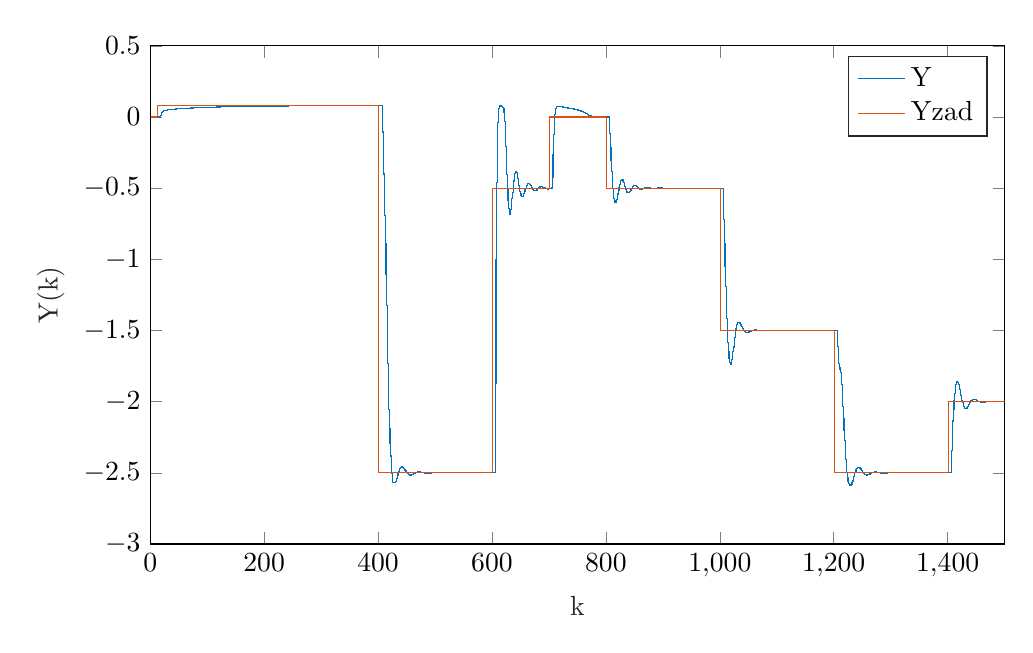
\begin{tikzpicture}

\begin{axis}[%
width=4.272in,
height=2.491in,
at={(0.717in,0.423in)},
scale only axis,
xmin=0,
xmax=1500,
xlabel style={font=\color{white!15!black}},
xlabel={k},
ymin=-3,
ymax=0.5,
ylabel style={font=\color{white!15!black}},
ylabel={Y(k)},
axis background/.style={fill=white},
legend style={legend cell align=left, align=left, draw=white!15!black}
]
\addplot[const plot, color=mycolor1] table[row sep=crcr] {%
1	0\\
2	0\\
3	0\\
4	0\\
5	0\\
6	0\\
7	0\\
8	0\\
9	0\\
10	0\\
11	0\\
12	0\\
13	0\\
14	0\\
15	0\\
16	0\\
17	0.00377487582098053\\
18	0.0121165796854498\\
19	0.0215102172004337\\
20	0.029415268100571\\
21	0.0350574468436003\\
22	0.038704892965461\\
23	0.0410047643538362\\
24	0.0425749073919599\\
25	0.0438365165894769\\
26	0.0449954572039627\\
27	0.0461018001651179\\
28	0.0471332846120104\\
29	0.0480599905615755\\
30	0.0488742460796323\\
31	0.0495922329158311\\
32	0.0502416258365108\\
33	0.0508478585269698\\
34	0.0514262702166614\\
35	0.0519816340424168\\
36	0.0525124443701629\\
37	0.0530160594225352\\
38	0.0534919753967575\\
39	0.0539424165854482\\
40	0.0543712053878993\\
41	0.0547821694658595\\
42	0.0551780648872473\\
43	0.055560357702681\\
44	0.0559296421980844\\
45	0.0562862468065266\\
46	0.0566306637086693\\
47	0.0569636693506257\\
48	0.0572862080373856\\
49	0.057599198139614\\
50	0.0579033940441375\\
51	0.0581993550597449\\
52	0.0584874976654977\\
53	0.0587681744234323\\
54	0.0590417317558171\\
55	0.0593085284433446\\
56	0.0595689237197802\\
57	0.0598232554513302\\
58	0.0600718253147312\\
59	0.0603148970753768\\
60	0.060552704545895\\
61	0.0607854620222123\\
62	0.0610133716052068\\
63	0.0612366257534156\\
64	0.0614554065998869\\
65	0.0616698845786504\\
66	0.0618802180855254\\
67	0.062086554463329\\
68	0.0622890685260655\\
69	0.0624881954159579\\
70	0.0626843520108916\\
71	0.0628778188554504\\
72	0.0630687720804198\\
73	0.0632573270227675\\
74	0.0634435668217181\\
75	0.0636275568226991\\
76	0.0638093514651422\\
77	0.0639889979853721\\
78	0.0641665386727272\\
79	0.0643420123153291\\
80	0.0645154551221673\\
81	0.0646869013012038\\
82	0.0648563834212525\\
83	0.0650239326447238\\
84	0.0651895788860116\\
85	0.0653533509275988\\
86	0.0655152765117112\\
87	0.0656753824171189\\
88	0.0658336945261981\\
89	0.0659902378849953\\
90	0.0661450367578258\\
91	0.0662981146773086\\
92	0.0664494944904247\\
93	0.066599198401016\\
94	0.0667472480090523\\
95	0.0668936643469396\\
96	0.0670384679131098\\
97	0.0671816787031062\\
98	0.0673233162383598\\
99	0.0674633995928354\\
100	0.0676019474177122\\
101	0.067738977964248\\
102	0.0678745091049684\\
103	0.0680085583533074\\
104	0.0681411428818188\\
105	0.0682722795390664\\
106	0.0684019848652941\\
107	0.0685302751069684\\
108	0.0686571662302789\\
109	0.0687826739336755\\
110	0.0689068136595155\\
111	0.0690296006048883\\
112	0.0691510497316784\\
113	0.0692711757759261\\
114	0.0693899932565369\\
115	0.0695075164833904\\
116	0.0696237595648929\\
117	0.0697387364150156\\
118	0.0698524607598577\\
119	0.0699649461437695\\
120	0.0700762059350687\\
121	0.0701862533313811\\
122	0.0702951013646326\\
123	0.0704027629057205\\
124	0.0705092506688859\\
125	0.070614577215812\\
126	0.0707187549594673\\
127	0.0708217961677132\\
128	0.070923712966694\\
129	0.0710245173440252\\
130	0.0711242211517957\\
131	0.0712228361093976\\
132	0.0713203738061959\\
133	0.0714168457040516\\
134	0.0715122631397076\\
135	0.0716066373270485\\
136	0.0716999793592442\\
137	0.0717923002107842\\
138	0.0718836107394133\\
139	0.0719739216879734\\
140	0.0720632436861609\\
141	0.072151587252204\\
142	0.0722389627944668\\
143	0.0723253806129857\\
144	0.072410850900943\\
145	0.0724953837460815\\
146	0.0725789891320662\\
147	0.0726616769397952\\
148	0.0727434569486647\\
149	0.0728243388377908\\
150	0.0729043321871916\\
151	0.0729834464789324\\
152	0.0730616910982364\\
153	0.0731390753345637\\
154	0.0732156083826606\\
155	0.0732912993435818\\
156	0.0733661572256861\\
157	0.0734401909456093\\
158	0.0735134093292142\\
159	0.0735858211125201\\
160	0.0736574349426132\\
161	0.0737282593785387\\
162	0.0737983028921762\\
163	0.0738675738690987\\
164	0.0739360806094181\\
165	0.0740038313286153\\
166	0.0740708341583583\\
167	0.0741370971473075\\
168	0.0742026282619093\\
169	0.0742674353871793\\
170	0.0743315263274748\\
171	0.074394908807257\\
172	0.0744575904718452\\
173	0.0745195788881602\\
174	0.0745808815454615\\
175	0.0746415058560744\\
176	0.0747014591561107\\
177	0.0747607487061817\\
178	0.0748193816921033\\
179	0.0748773652255958\\
180	0.0749347063449753\\
181	0.0749914120158406\\
182	0.075047489131752\\
183	0.0751029445149059\\
184	0.075157784916802\\
185	0.0752120170189061\\
186	0.0752656474333067\\
187	0.0753186827033662\\
188	0.0753711293043668\\
189	0.0754229936441518\\
190	0.0754742820637606\\
191	0.0755250008380603\\
192	0.0755751561763705\\
193	0.0756247542230849\\
194	0.0756738010582872\\
195	0.0757223026983624\\
196	0.0757702650966035\\
197	0.0758176941438133\\
198	0.0758645956689022\\
199	0.075910975439481\\
200	0.0759568391624488\\
201	0.0760021924845772\\
202	0.0760470409930897\\
203	0.0760913902162364\\
204	0.0761352456238647\\
205	0.0761786126279853\\
206	0.0762214965833341\\
207	0.0762639027879297\\
208	0.0763058364836262\\
209	0.0763473028566623\\
210	0.0763883070382057\\
211	0.0764288541048933\\
212	0.0764689490793673\\
213	0.0765085969308067\\
214	0.0765478025754551\\
215	0.0765865708771439\\
216	0.0766249066478111\\
217	0.076662814648017\\
218	0.0767002995874538\\
219	0.0767373661254533\\
220	0.0767740188714886\\
221	0.0768102623856729\\
222	0.0768461011792531\\
223	0.0768815397151007\\
224	0.0769165824081971\\
225	0.076951233626116\\
226	0.0769854976895009\\
227	0.0770193788725394\\
228	0.0770528814034326\\
229	0.0770860094648611\\
230	0.0771187671944469\\
231	0.0771511586852109\\
232	0.0771831879860272\\
233	0.0772148591020726\\
234	0.0772461759952731\\
235	0.0772771425847453\\
236	0.0773077627472353\\
237	0.0773380403175525\\
238	0.0773679790890004\\
239	0.0773975828138029\\
240	0.0774268552035275\\
241	0.077455799929504\\
242	0.0774844206232398\\
243	0.0775127208768314\\
244	0.0775407042433721\\
245	0.0775683742373562\\
246	0.0775957343350789\\
247	0.0776227879750334\\
248	0.0776495385583036\\
249	0.0776759894489535\\
250	0.0777021439744128\\
251	0.0777280054258595\\
252	0.077753577058598\\
253	0.0777788620924342\\
254	0.0778038637120474\\
255	0.0778285850673578\\
256	0.0778530292738912\\
257	0.0778771994131403\\
258	0.077901098532922\\
259	0.0779247296477318\\
260	0.0779480957390946\\
261	0.0779711997559124\\
262	0.0779940446148079\\
263	0.078016633200466\\
264	0.0780389683659708\\
265	0.0780610529331402\\
266	0.0780828896928565\\
267	0.0781044814053949\\
268	0.0781258308007474\\
269	0.0781469405789447\\
270	0.0781678134103742\\
271	0.0781884519360952\\
272	0.0782088587681512\\
273	0.0782290364898786\\
274	0.0782489876562127\\
275	0.0782687147939907\\
276	0.0782882204022515\\
277	0.0783075069525325\\
278	0.0783265768891639\\
279	0.0783454326295594\\
280	0.0783640765645044\\
281	0.0783825110584413\\
282	0.0784007384497519\\
283	0.0784187610510366\\
284	0.0784365811493917\\
285	0.0784542010066828\\
286	0.078471622859816\\
287	0.0784888489210069\\
288	0.0785058813780454\\
289	0.0785227223945594\\
290	0.0785393741102749\\
291	0.0785558386412737\\
292	0.0785721180802481\\
293	0.0785882144967541\\
294	0.0786041299374605\\
295	0.0786198664263967\\
296	0.0786354259651972\\
297	0.0786508105333439\\
298	0.078666022088406\\
299	0.0786810625662774\\
300	0.078695933881411\\
301	0.0787106379270518\\
302	0.0787251765754664\\
303	0.078739551678171\\
304	0.0787537650661566\\
305	0.0787678185501118\\
306	0.0787817139206436\\
307	0.0787954529484957\\
308	0.0788090373847647\\
309	0.0788224689611134\\
310	0.0788357493899832\\
311	0.0788488803648029\\
312	0.0788618635601959\\
313	0.0788747006321857\\
314	0.0788873932183981\\
315	0.0788999429382626\\
316	0.0789123513932107\\
317	0.0789246201668724\\
318	0.0789367508252709\\
319	0.0789487449170149\\
320	0.0789606039734891\\
321	0.0789723295090426\\
322	0.0789839230211753\\
323	0.0789953859907223\\
324	0.0790067198820366\\
325	0.0790179261431693\\
326	0.0790290062060488\\
327	0.0790399614866571\\
328	0.0790507933852047\\
329	0.079061503286304\\
330	0.0790720925591404\\
331	0.0790825625576411\\
332	0.0790929146206437\\
333	0.0791031500720611\\
334	0.0791132702210459\\
335	0.0791232763621526\\
336	0.0791331697754984\\
337	0.0791429517269215\\
338	0.0791526234681387\\
339	0.0791621862369005\\
340	0.0791716412571455\\
341	0.0791809897391516\\
342	0.0791902328796873\\
343	0.0791993718621603\\
344	0.0792084078567647\\
345	0.079217342020627\\
346	0.0792261754979498\\
347	0.079234909420155\\
348	0.0792435449060244\\
349	0.0792520830618394\\
350	0.079260524981519\\
351	0.0792688717467566\\
352	0.0792771244271545\\
353	0.0792852840803583\\
354	0.0792933517521884\\
355	0.0793013284767715\\
356	0.079309215276669\\
357	0.0793170131630057\\
358	0.079324723135596\\
359	0.0793323461830694\\
360	0.079339883282994\\
361	0.0793473354019991\\
362	0.0793547034958965\\
363	0.0793619885098001\\
364	0.0793691913782449\\
365	0.0793763130253037\\
366	0.0793833543647034\\
367	0.0793903162999398\\
368	0.0793971997243908\\
369	0.0794040055214291\\
370	0.0794107345645327\\
371	0.079417387717395\\
372	0.0794239658340335\\
373	0.0794304697588971\\
374	0.0794369003269723\\
375	0.0794432583638884\\
376	0.0794495446860218\\
377	0.079455760100598\\
378	0.079461905405794\\
379	0.0794679813908389\\
380	0.0794739888361129\\
381	0.079479928513246\\
382	0.0794858011852154\\
383	0.0794916076064418\\
384	0.0794973485228842\\
385	0.0795030246721347\\
386	0.079508636783511\\
387	0.0795141855781489\\
388	0.0795196717690935\\
389	0.0795250960613888\\
390	0.0795304591521673\\
391	0.0795357617307382\\
392	0.0795410044786739\\
393	0.0795461880698972\\
394	0.0795513131707655\\
395	0.079556380440156\\
396	0.0795613905295489\\
397	0.0795663440831094\\
398	0.0795712417377698\\
399	0.0795760841233101\\
400	0.0795808718624378\\
401	0.0795856055708664\\
402	0.0795902858573942\\
403	0.0795949133239807\\
404	0.0795994885658236\\
405	0.0796040121714339\\
406	0.0824887733208591\\
407	0.0323235216515027\\
408	-0.105714480732642\\
409	-0.262369438664933\\
410	-0.400807317171615\\
411	-0.53428156136025\\
412	-0.692679207740456\\
413	-0.887817177601582\\
414	-1.10512165738977\\
415	-1.32579553798256\\
416	-1.5373793620982\\
417	-1.73219396781449\\
418	-1.90607787571779\\
419	-2.0573819515545\\
420	-2.1861836872046\\
421	-2.29368524624664\\
422	-2.38176243397639\\
423	-2.45240921080409\\
424	-2.50716604859443\\
425	-2.54764136534908\\
426	-2.56650372506516\\
427	-2.57076138037403\\
428	-2.56965019471301\\
429	-2.56738112096477\\
430	-2.56473313273632\\
431	-2.55972342928915\\
432	-2.55040317859488\\
433	-2.53701292691691\\
434	-2.52144435078915\\
435	-2.50592738733226\\
436	-2.49209262796096\\
437	-2.48069045498971\\
438	-2.47182893566643\\
439	-2.46532908514341\\
440	-2.46098769367\\
441	-2.45868654498756\\
442	-2.45835876965695\\
443	-2.4598982968126\\
444	-2.4630945517685\\
445	-2.46762631933669\\
446	-2.47341835987301\\
447	-2.47982703250461\\
448	-2.48619521465202\\
449	-2.49218297669136\\
450	-2.49765241160709\\
451	-2.50258917425486\\
452	-2.5069537866261\\
453	-2.51061188921296\\
454	-2.51340297547702\\
455	-2.51522573631538\\
456	-2.51607847181688\\
457	-2.51604856542785\\
458	-2.51527291443114\\
459	-2.51390152844061\\
460	-2.51207794170131\\
461	-2.50993486230667\\
462	-2.50759776137791\\
463	-2.50518808862775\\
464	-2.50282187575094\\
465	-2.50060425623802\\
466	-2.49861169890349\\
467	-2.49692167784116\\
468	-2.49558700944886\\
469	-2.49462469744028\\
470	-2.49402664743619\\
471	-2.49376788152745\\
472	-2.49381608941615\\
473	-2.49413561799123\\
474	-2.4946850340804\\
475	-2.49541538389374\\
476	-2.49627185471408\\
477	-2.49719810477203\\
478	-2.49814114848372\\
479	-2.49905476296454\\
480	-2.49990095015352\\
481	-2.50065005540592\\
482	-2.50128034488651\\
483	-2.50177760557219\\
484	-2.50213489017622\\
485	-2.50235222656057\\
486	-2.50243645952178\\
487	-2.50239901685928\\
488	-2.50225578012705\\
489	-2.50202620393065\\
490	-2.50173153372342\\
491	-2.5013933503599\\
492	-2.50103230565256\\
493	-2.50066733297885\\
494	-2.50031528035933\\
495	-2.49999058995146\\
496	-2.49970493049851\\
497	-2.49946687127845\\
498	-2.49928172675552\\
499	-2.49915165023168\\
500	-2.49907594354501\\
501	-2.49905149266602\\
502	-2.49907324663151\\
503	-2.49913469145999\\
504	-2.49922830551721\\
505	-2.499345998453\\
506	-2.49947951859682\\
507	-2.49962089509687\\
508	-2.49976273378263\\
509	-2.49989847801147\\
510	-2.50002263380009\\
511	-2.50013090485692\\
512	-2.50022025110374\\
513	-2.50028886942238\\
514	-2.50033611247319\\
515	-2.50036237339147\\
516	-2.50036894777274\\
517	-2.50035787568534\\
518	-2.50033176613055\\
519	-2.50029361036623\\
520	-2.50024659575653\\
521	-2.500193932509\\
522	-2.50013870230353\\
523	-2.50008373346244\\
524	-2.50003150387552\\
525	-2.49998407122888\\
526	-2.4999430301566\\
527	-2.49990949238347\\
528	-2.499884094633\\
529	-2.49986702627538\\
530	-2.4998580729483\\
531	-2.4998566743404\\
532	-2.49986199121807\\
533	-2.4998729776827\\
534	-2.49988845434109\\
535	-2.49990717822628\\
536	-2.4999279067542\\
537	-2.49994945394283\\
538	-2.49997073760511\\
539	-2.49999081652324\\
540	-2.50000891690472\\
541	-2.50002444794938\\
542	-2.50003700701247\\
543	-2.50004637541607\\
544	-2.50005250633324\\
545	-2.50005550633493\\
546	-2.50005561219964\\
547	-2.50005316467651\\
548	-2.50004858047877\\
549	-2.50004232417771\\
550	-2.50003488130097\\
551	-2.50002673363828\\
552	-2.50001833765641\\
553	-2.50001010663783\\
554	-2.50000239693288\\
555	-2.49999549848746\\
556	-2.49998962955449\\
557	-2.49998493530666\\
558	-2.49998148993409\\
559	-2.49997930171769\\
560	-2.49997832050535\\
561	-2.49997844697474\\
562	-2.49997954304779\\
563	-2.49998144283733\\
564	-2.49998396355466\\
565	-2.49998691588045\\
566	-2.49999011339127\\
567	-2.4999933807236\\
568	-2.49999656026538\\
569	-2.4999995172373\\
570	-2.50000214312298\\
571	-2.50000435749158\\
572	-2.50000610831936\\
573	-2.50000737097491\\
574	-2.50000814607339\\
575	-2.5000084564323\\
576	-2.50000834337599\\
577	-2.50000786263687\\
578	-2.50000708008881\\
579	-2.50000606752748\\
580	-2.50000489868367\\
581	-2.5000036456237\\
582	-2.50000237565518\\
583	-2.50000114881958\\
584	-2.5000000160166\\
585	-2.49999901777059\\
586	-2.49999818361851\\
587	-2.49999753207299\\
588	-2.49999707109308\\
589	-2.49999679898095\\
590	-2.49999670561268\\
591	-2.49999677390708\\
592	-2.49999698143691\\
593	-2.49999730209201\\
594	-2.4999977077121\\
595	-2.49999816961818\\
596	-2.49999865998489\\
597	-2.49999915300974\\
598	-2.4999996258504\\
599	-2.50000005931465\\
600	-2.50000043830131\\
601	-2.50000075200161\\
602	-2.50000099388039\\
603	-2.50000116146433\\
604	-2.50000125596985\\
605	-2.50000128180688\\
606	-1.87468317927404\\
607	-1.00153019406062\\
608	-0.45742160471741\\
609	-0.174148023924221\\
610	-0.0356951989163385\\
611	0.0302275491956203\\
612	0.061255508826796\\
613	0.0755111829251453\\
614	0.080994625735553\\
615	0.0813572021474004\\
616	0.0788295495545531\\
617	0.0748426743764155\\
618	0.0702408936150992\\
619	0.0655088815949336\\
620	0.0584273024503272\\
621	0.0307892031396256\\
622	-0.0294332760061986\\
623	-0.112399888406416\\
624	-0.206267752799954\\
625	-0.304198536975389\\
626	-0.405988129764884\\
627	-0.502901812343609\\
628	-0.583176245829649\\
629	-0.64009562659945\\
630	-0.672721282402001\\
631	-0.682667907061504\\
632	-0.672838985174179\\
633	-0.647903949567414\\
634	-0.612912280764493\\
635	-0.572268934308342\\
636	-0.529571978233946\\
637	-0.487878182202985\\
638	-0.450049588315347\\
639	-0.418787164364279\\
640	-0.396364679802554\\
641	-0.38427340573527\\
642	-0.382916072357299\\
643	-0.391468366756835\\
644	-0.408025117211148\\
645	-0.430029436253875\\
646	-0.454653658167063\\
647	-0.479715942749651\\
648	-0.503435898945801\\
649	-0.524228364320335\\
650	-0.540813636737023\\
651	-0.552380044190397\\
652	-0.558625632622153\\
653	-0.559686156606954\\
654	-0.556084802122422\\
655	-0.548637356195936\\
656	-0.538327842270179\\
657	-0.526202831093901\\
658	-0.513296682371612\\
659	-0.500588772625915\\
660	-0.488974738543211\\
661	-0.479229787635598\\
662	-0.471958780358088\\
663	-0.467543874986777\\
664	-0.466107136507684\\
665	-0.467502736015461\\
666	-0.471349988423323\\
667	-0.477073732404492\\
668	-0.484000162587345\\
669	-0.491442916849548\\
670	-0.498761360162275\\
671	-0.505401086700038\\
672	-0.510923261163109\\
673	-0.515024184547775\\
674	-0.517541334251457\\
675	-0.518449467055883\\
676	-0.517847883204649\\
677	-0.515939444631444\\
678	-0.513003933387433\\
679	-0.509368514513924\\
680	-0.505378327298035\\
681	-0.501369787325785\\
682	-0.497647934428171\\
683	-0.49446819933184\\
684	-0.492022624296111\\
685	-0.490430761560081\\
686	-0.489735641674074\\
687	-0.489906560750272\\
688	-0.490846451901739\\
689	-0.492405289556248\\
690	-0.494398008377623\\
691	-0.496623900013984\\
692	-0.498884995330553\\
693	-0.5010017154856\\
694	-0.50282498309606\\
695	-0.504244315083487\\
696	-0.505191940085788\\
697	-0.505643272712379\\
698	-0.5056141724595\\
699	-0.505155542880968\\
700	-0.504345908579984\\
701	-0.503282678662023\\
702	-0.502072862802367\\
703	-0.500823994288679\\
704	-0.499635926076146\\
705	-0.498594020456585\\
706	-0.426119404184766\\
707	-0.266193966915896\\
708	-0.123030061891784\\
709	-0.0317574192032682\\
710	0.0183397603560901\\
711	0.0449099721210851\\
712	0.0593828332999315\\
713	0.0673886417100853\\
714	0.0716735577430898\\
715	0.0737475540825154\\
716	0.0745226013048691\\
717	0.0745582240889412\\
718	0.07418838321292\\
719	0.0736049860966633\\
720	0.0729144294966101\\
721	0.0721738895849246\\
722	0.0714132646269267\\
723	0.0706477961326787\\
724	0.0698850432000291\\
725	0.0691286139273673\\
726	0.0683801096161342\\
727	0.0676401153900089\\
728	0.0669086946264463\\
729	0.0661856311698508\\
730	0.0654705451412326\\
731	0.0647629463867131\\
732	0.0640622575896159\\
733	0.0633678228927034\\
734	0.0626787412721196\\
735	0.0619916022716446\\
736	0.0613009966055501\\
737	0.0606017965735132\\
738	0.0598907133460981\\
739	0.0591667420725188\\
740	0.0584301122010527\\
741	0.0576804395661473\\
742	0.0569153173237185\\
743	0.0561301738883856\\
744	0.055319311546701\\
745	0.0544773217451619\\
746	0.0535999659746272\\
747	0.0526840502724719\\
748	0.0517264649665659\\
749	0.0507230276180891\\
750	0.0496678141737269\\
751	0.0485533130913776\\
752	0.0473712470050765\\
753	0.0461135800171799\\
754	0.044773224164533\\
755	0.0433442275566184\\
756	0.0418215786698496\\
757	0.0402009865333765\\
758	0.0384789834588075\\
759	0.0366534856352115\\
760	0.034724686901071\\
761	0.0326960058067471\\
762	0.0305748203370198\\
763	0.0283742070532992\\
764	0.0261145171177655\\
765	0.0238209031419268\\
766	0.0215206483465246\\
767	0.0192421289011435\\
768	0.0170141945131599\\
769	0.0148652901009807\\
770	0.0128221974665909\\
771	0.010908708032183\\
772	0.00914452551632815\\
773	0.00754450458202718\\
774	0.00611820766160545\\
775	0.00486973527151727\\
776	0.00379781538043557\\
777	0.00289616574155657\\
778	0.00215413528048815\\
779	0.001557591142227\\
780	0.00108997211923767\\
781	0.000733400346595181\\
782	0.000469740826534428\\
783	0.000281518426495293\\
784	0.000152633897428202\\
785	6.88540122919566e-05\\
786	1.80796790716752e-05\\
787	-9.58287335482271e-06\\
788	-2.19093878869685e-05\\
789	-2.47587753151055e-05\\
790	-2.23436262184657e-05\\
791	-1.75301758359397e-05\\
792	-1.21357137319637e-05\\
793	-7.20070170187823e-06\\
794	-3.22200026391399e-06\\
795	-3.41465582828853e-07\\
796	1.50985121388982e-06\\
797	2.50772023245363e-06\\
798	2.86463350982168e-06\\
799	2.78651422497086e-06\\
800	2.44938145869395e-06\\
801	1.98992056635619e-06\\
802	1.50498919619355e-06\\
803	1.0562316523808e-06\\
804	6.77042264074099e-07\\
805	3.80034598046243e-07\\
806	-0.036316112845438\\
807	-0.119134879417458\\
808	-0.215202689595387\\
809	-0.305964668803316\\
810	-0.383562800458848\\
811	-0.447669855526009\\
812	-0.499705146200304\\
813	-0.540518926571536\\
814	-0.570508345682499\\
815	-0.58998467505882\\
816	-0.599575454233833\\
817	-0.600287063646109\\
818	-0.593346787926651\\
819	-0.580096843547725\\
820	-0.562018586224645\\
821	-0.540795950348766\\
822	-0.518287787294812\\
823	-0.49637317106689\\
824	-0.476748821865876\\
825	-0.460774524511618\\
826	-0.448259931485401\\
827	-0.440474112350802\\
828	-0.438434272676662\\
829	-0.441998102759906\\
830	-0.450199731842574\\
831	-0.461560499389351\\
832	-0.474584895683728\\
833	-0.487996933892094\\
834	-0.5007514546298\\
835	-0.512006927092293\\
836	-0.521108799041982\\
837	-0.527606060122569\\
838	-0.531281662028555\\
839	-0.532162581887765\\
840	-0.530494388854117\\
841	-0.526687848231407\\
842	-0.5212572800787\\
843	-0.514767427873625\\
844	-0.507793939094259\\
845	-0.50089277597292\\
846	-0.49461567313138\\
847	-0.489350407528347\\
848	-0.485377533834073\\
849	-0.482890691473136\\
850	-0.481965305106058\\
851	-0.482548279495983\\
852	-0.484456301951091\\
853	-0.487401320738829\\
854	-0.491034437953493\\
855	-0.494989838856553\\
856	-0.498920949188558\\
857	-0.502525686147776\\
858	-0.505562151311295\\
859	-0.507857780279232\\
860	-0.509313680796907\\
861	-0.509904425483782\\
862	-0.509672963952619\\
863	-0.508720716163962\\
864	-0.507193813077313\\
865	-0.505267149630666\\
866	-0.503126457472185\\
867	-0.500958166868423\\
868	-0.498932190953318\\
869	-0.497189464410775\\
870	-0.495835349160116\\
871	-0.494935553893258\\
872	-0.494515346725152\\
873	-0.494561061145151\\
874	-0.495024000151727\\
875	-0.495827080069923\\
876	-0.496873619363737\\
877	-0.498057243322379\\
878	-0.499271684614948\\
879	-0.500419403415062\\
880	-0.501418354268025\\
881	-0.502206624615177\\
882	-0.502744950240261\\
883	-0.503017263213614\\
884	-0.503029493110205\\
885	-0.502806884823672\\
886	-0.502390204902309\\
887	-0.501830901526988\\
888	-0.501186261012255\\
889	-0.50051449750737\\
890	-0.499870132985051\\
891	-0.499300151238823\\
892	-0.498841109126389\\
893	-0.498517367110787\\
894	-0.498340445348219\\
895	-0.498309406295763\\
896	-0.498412137003199\\
897	-0.498627362511328\\
898	-0.498927184354957\\
899	-0.499279907020004\\
900	-0.499652898224151\\
901	-0.500015240916555\\
902	-0.500339975811068\\
903	-0.500605793703576\\
904	-0.500798104023736\\
905	-0.500909468503128\\
906	-0.500939438071993\\
907	-0.500893882980521\\
908	-0.500783897154231\\
909	-0.500624420273233\\
910	-0.500432709336268\\
911	-0.500226782120377\\
912	-0.500023955343235\\
913	-0.4998395788893\\
914	-0.499686045673675\\
915	-0.499572128756543\\
916	-0.499502664738468\\
917	-0.499478573020628\\
918	-0.499497175480606\\
919	-0.499552761878481\\
920	-0.499637333401635\\
921	-0.499741449784322\\
922	-0.499855104355678\\
923	-0.499968556082144\\
924	-0.500073057665686\\
925	-0.500161432970896\\
926	-0.500228473939543\\
927	-0.500271144218679\\
928	-0.500288594674418\\
929	-0.50028200836849\\
930	-0.500254304536534\\
931	-0.500209739031312\\
932	-0.500153442194678\\
933	-0.50009093583741\\
934	-0.500027668337684\\
935	-0.499968601647267\\
936	-0.499917876866339\\
937	-0.499878576455157\\
938	-0.499852591924345\\
939	-0.499840596782058\\
940	-0.499842116341102\\
941	-0.499855679303821\\
942	-0.499879031222765\\
943	-0.499909387148129\\
944	-0.49994370001247\\
945	-0.499978922418774\\
946	-0.500012242222832\\
947	-0.500041276301174\\
948	-0.500064211654654\\
949	-0.500079888253154\\
950	-0.50008782308752\\
951	-0.500088179495582\\
952	-0.500081689668354\\
953	-0.50006954104156\\
954	-0.500053238972948\\
955	-0.500034458673391\\
956	-0.500014898873483\\
957	-0.499996148323775\\
958	-0.499979574135732\\
959	-0.49996623839681\\
960	-0.499956846677181\\
961	-0.499951729224718\\
962	-0.499950853038165\\
963	-0.499953860799201\\
964	-0.499960130966558\\
965	-0.499968852267787\\
966	-0.49997910538827\\
967	-0.499989944821626\\
968	-0.500000474540383\\
969	-0.500009912256545\\
970	-0.500017638449901\\
971	-0.500023227903933\\
972	-0.500026463067887\\
973	-0.500027330037476\\
974	-0.500025999210073\\
975	-0.500022793647186\\
976	-0.500018148821173\\
977	-0.500012567718243\\
978	-0.50000657522892\\
979	-0.500000675417617\\
980	-0.499995314681055\\
981	-0.49999085304992\\
982	-0.499987545034479\\
983	-0.499985530538286\\
984	-0.499984835534231\\
985	-0.499985381473523\\
986	-0.499987001826316\\
987	-0.499989463761703\\
988	-0.499992492777051\\
989	-0.499995798078218\\
990	-0.499999096674508\\
991	-0.500002134455655\\
992	-0.500004702925128\\
993	-0.50000665073263\\
994	-0.500007889636394\\
995	-0.500008394993281\\
996	-0.500008201287533\\
997	-0.500007393540997\\
998	-0.500006095681154\\
999	-0.500004457070298\\
1000	-0.500002638420458\\
1001	-0.500000798243369\\
1002	-0.499999080828234\\
1003	-0.499997606522618\\
1004	-0.499996464836325\\
1005	-0.49999571061804\\
1006	-0.573093976874\\
1007	-0.71844997423333\\
1008	-0.887626673440462\\
1009	-1.04979148823048\\
1010	-1.19029243355149\\
1011	-1.30964228274774\\
1012	-1.41335080036371\\
1013	-1.50450645399568\\
1014	-1.58286479025206\\
1015	-1.64644548935894\\
1016	-1.69347933674394\\
1017	-1.72351939932669\\
1018	-1.7375519085697\\
1019	-1.73756358585914\\
1020	-1.72603270997922\\
1021	-1.70557727853194\\
1022	-1.6787712277748\\
1023	-1.64804943584158\\
1024	-1.61563611928647\\
1025	-1.58347453512599\\
1026	-1.5494656286526\\
1027	-1.51697742869053\\
1028	-1.48974318074385\\
1029	-1.46919456467504\\
1030	-1.4551932437151\\
1031	-1.44662301737137\\
1032	-1.44227906407552\\
1033	-1.44131962851921\\
1034	-1.44320445636474\\
1035	-1.44748868933222\\
1036	-1.45366872801044\\
1037	-1.46115204729619\\
1038	-1.46931717365742\\
1039	-1.4775934541166\\
1040	-1.48551466642211\\
1041	-1.49273549075332\\
1042	-1.49902236572004\\
1043	-1.50423517993878\\
1044	-1.5083102858794\\
1045	-1.51124769399106\\
1046	-1.51322435903767\\
1047	-1.51423340497004\\
1048	-1.51428733448312\\
1049	-1.51352602680043\\
1050	-1.5121573525773\\
1051	-1.51040773978976\\
1052	-1.50846800907641\\
1053	-1.50647470307231\\
1054	-1.50452406985374\\
1055	-1.50269065659156\\
1056	-1.50103766187986\\
1057	-1.49961699816114\\
1058	-1.49846432379373\\
1059	-1.4975953132092\\
1060	-1.49700594562728\\
1061	-1.49667624084824\\
1062	-1.4965753884012\\
1063	-1.49666647769933\\
1064	-1.49691005035316\\
1065	-1.49726654017003\\
1066	-1.49769367324745\\
1067	-1.49816138740757\\
1068	-1.49864311951086\\
1069	-1.49911187374925\\
1070	-1.49954388057156\\
1071	-1.49992105006014\\
1072	-1.5002328060515\\
1073	-1.5004755871389\\
1074	-1.50065068393184\\
1075	-1.50076224778162\\
1076	-1.50081613860645\\
1077	-1.50081951572975\\
1078	-1.50078069030018\\
1079	-1.50070882857397\\
1080	-1.50061341534006\\
1081	-1.50050361604464\\
1082	-1.50038772466783\\
1083	-1.50027280704974\\
1084	-1.50016454513964\\
1085	-1.50006722584793\\
1086	-1.49998396258363\\
1087	-1.49991628144849\\
1088	-1.49986469258873\\
1089	-1.49982901944635\\
1090	-1.49980838547266\\
1091	-1.49980128071754\\
1092	-1.4998056728682\\
1093	-1.49981921955935\\
1094	-1.49983951989433\\
1095	-1.49986430150291\\
1096	-1.49989152050432\\
1097	-1.49991939801163\\
1098	-1.49994643167223\\
1099	-1.4999714074408\\
1100	-1.49999341324409\\
1101	-1.50001184384213\\
1102	-1.50002638752885\\
1103	-1.50003699349788\\
1104	-1.50004382594101\\
1105	-1.50004721330501\\
1106	-1.50004759394957\\
1107	-1.50004549211549\\
1108	-1.50004146054434\\
1109	-1.50003604182675\\
1110	-1.50002975102648\\
1111	-1.50002305925217\\
1112	-1.50001637989261\\
1113	-1.500010055466\\
1114	-1.50000434832935\\
1115	-1.49999943941811\\
1116	-1.49999543423972\\
1117	-1.49999237307787\\
1118	-1.49999024228293\\
1119	-1.49998898492336\\
1120	-1.49998851066465\\
1121	-1.49998870535381\\
1122	-1.4999894405218\\
1123	-1.49999058247883\\
1124	-1.49999200037456\\
1125	-1.49999357267882\\
1126	-1.49999519204094\\
1127	-1.49999676747948\\
1128	-1.49999822668311\\
1129	-1.49999951648951\\
1130	-1.50000060174941\\
1131	-1.50000146372604\\
1132	-1.50000209810718\\
1133	-1.50000251284291\\
1134	-1.50000272578042\\
1135	-1.50000276204995\\
1136	-1.50000265139655\\
1137	-1.50000242571317\\
1138	-1.50000211696438\\
1139	-1.50000175556533\\
1140	-1.50000136917564\\
1141	-1.5000009818387\\
1142	-1.5000006134184\\
1143	-1.50000027931424\\
1144	-1.49999999044363\\
1145	-1.4999997534654\\
1146	-1.49999957119005\\
1147	-1.49999944315723\\
1148	-1.49999936622127\\
1149	-1.49999933518761\\
1150	-1.49999934346045\\
1151	-1.49999938363165\\
1152	-1.49999944799817\\
1153	-1.49999952899543\\
1154	-1.49999961954851\\
1155	-1.49999971334567\\
1156	-1.4999998050309\\
1157	-1.49999989031295\\
1158	-1.49999996599603\\
1159	-1.50000002994444\\
1160	-1.50000008099832\\
1161	-1.50000011885658\\
1162	-1.50000014393978\\
1163	-1.50000015724229\\
1164	-1.50000016018148\\
1165	-1.50000015445106\\
1166	-1.5000001418856\\
1167	-1.50000012434031\\
1168	-1.50000010359368\\
1169	-1.50000008127067\\
1170	-1.50000005878678\\
1171	-1.50000003731336\\
1172	-1.50000001776185\\
1173	-1.50000000078419\\
1174	-1.49999998678602\\
1175	-1.49999997594967\\
1176	-1.49999996826418\\
1177	-1.49999996355997\\
1178	-1.49999996154567\\
1179	-1.49999996184492\\
1180	-1.4999999640308\\
1181	-1.49999996765661\\
1182	-1.49999997228201\\
1183	-1.49999997749416\\
1184	-1.49999998292371\\
1185	-1.49999998825587\\
1186	-1.49999999323675\\
1187	-1.49999999767551\\
1188	-1.50000000144288\\
1189	-1.5000000044667\\
1190	-1.50000000672551\\
1191	-1.50000000824055\\
1192	-1.50000000906712\\
1193	-1.50000000928565\\
1194	-1.50000000899316\\
1195	-1.5000000082954\\
1196	-1.50000000729991\\
1197	-1.50000000611029\\
1198	-1.50000000482158\\
1199	-1.50000000351694\\
1200	-1.50000000226555\\
1201	-1.50000000112156\\
1202	-1.50000000012403\\
1203	-1.49999999929762\\
1204	-1.49999999865392\\
1205	-1.49999999819316\\
1206	-1.5422291345592\\
1207	-1.61485020735383\\
1208	-1.68482830262639\\
1209	-1.73470340365729\\
1210	-1.76062217274303\\
1211	-1.77476636772741\\
1212	-1.79366272221756\\
1213	-1.82815980654574\\
1214	-1.88173595074092\\
1215	-1.9524611680616\\
1216	-2.03358282761597\\
1217	-2.11772655827332\\
1218	-2.19953983695223\\
1219	-2.27564315607084\\
1220	-2.3441196408013\\
1221	-2.40410658196514\\
1222	-2.45547449018242\\
1223	-2.4984564638244\\
1224	-2.53343503999825\\
1225	-2.56084942822374\\
1226	-2.57762198504265\\
1227	-2.58597761617516\\
1228	-2.58921784618419\\
1229	-2.58897037610767\\
1230	-2.58576676149973\\
1231	-2.57937718838227\\
1232	-2.56964735179499\\
1233	-2.55704150664492\\
1234	-2.54255700021237\\
1235	-2.52738723276417\\
1236	-2.51261376504935\\
1237	-2.49905060574579\\
1238	-2.48723324262886\\
1239	-2.47748002295803\\
1240	-2.46995977177709\\
1241	-2.4647265086979\\
1242	-2.46173148359287\\
1243	-2.46083386687724\\
1244	-2.46181633874868\\
1245	-2.46440476139243\\
1246	-2.46841020216298\\
1247	-2.4734076946122\\
1248	-2.47894984244661\\
1249	-2.48470123028058\\
1250	-2.49040664716733\\
1251	-2.49586914615094\\
1252	-2.50091011505069\\
1253	-2.5053547526883\\
1254	-2.50905155449743\\
1255	-2.51189685271626\\
1256	-2.51384779877157\\
1257	-2.51491992658391\\
1258	-2.51517454382191\\
1259	-2.51470399495314\\
1260	-2.51361984182014\\
1261	-2.51204521599314\\
1262	-2.51010944296783\\
1263	-2.50794290621565\\
1264	-2.50567162529343\\
1265	-2.50341195163631\\
1266	-2.50126173086814\\
1267	-2.49931041796398\\
1268	-2.49762782837872\\
1269	-2.49625858744319\\
1270	-2.49522546402084\\
1271	-2.49453264591358\\
1272	-2.49416983723822\\
1273	-2.49411493656411\\
1274	-2.49433525480674\\
1275	-2.49478901722137\\
1276	-2.49542782412407\\
1277	-2.49619987758005\\
1278	-2.49705331493819\\
1279	-2.49793901917264\\
1280	-2.4988126481998\\
1281	-2.49963594544282\\
1282	-2.50037755174119\\
1283	-2.50101348750695\\
1284	-2.50152734835837\\
1285	-2.50191019541301\\
1286	-2.50216027767225\\
1287	-2.5022817963219\\
1288	-2.50228437442988\\
1289	-2.50218214772721\\
1290	-2.50199243076297\\
1291	-2.50173444973311\\
1292	-2.50142815191791\\
1293	-2.50109321917427\\
1294	-2.50074828441717\\
1295	-2.50041026702947\\
1296	-2.50009381143872\\
1297	-2.4998108562295\\
1298	-2.49957037198437\\
1299	-2.49937828640995\\
1300	-2.49923758163259\\
1301	-2.49914852698403\\
1302	-2.4991090056196\\
1303	-2.49911490140613\\
1304	-2.49916052285722\\
1305	-2.49923904571837\\
1306	-2.49934295078704\\
1307	-2.49946446824256\\
1308	-2.49959594730709\\
1309	-2.49973018622005\\
1310	-2.4998607161933\\
1311	-2.49998201378961\\
1312	-2.50008964269316\\
1313	-2.50018032408354\\
1314	-2.50025194326612\\
1315	-2.50030350485734\\
1316	-2.50033504552735\\
1317	-2.50034751171528\\
1318	-2.50034260989569\\
1319	-2.5003226383143\\
1320	-2.5002903104159\\
1321	-2.50024858006274\\
1322	-2.50020047718004\\
1323	-2.50014896029418\\
1324	-2.50009679034174\\
1325	-2.50004642853707\\
1326	-2.49999996004796\\
1327	-2.49995904282276\\
1328	-2.49992488338569\\
1329	-2.49989823571922\\
1330	-2.49987942042993\\
1331	-2.49986836171565\\
1332	-2.49986463817318\\
1333	-2.49986754353067\\
1334	-2.49987615318478\\
1335	-2.49988939258007\\
1336	-2.49990610410137\\
1337	-2.49992510972536\\
1338	-2.49994526719207\\
1339	-2.49996551793952\\
1340	-2.49998492554659\\
1341	-2.50000270399231\\
1342	-2.50001823561851\\
1343	-2.50003107921262\\
1344	-2.50004096905419\\
1345	-2.50004780607483\\
1346	-2.50005164247749\\
1347	-2.50005266132914\\
1348	-2.50005115255423\\
1349	-2.5000474869282\\
1350	-2.50004208950048\\
1351	-2.50003541369517\\
1352	-2.50002791720159\\
1353	-2.50002004054265\\
1354	-2.50001218898875\\
1355	-2.50000471825283\\
1356	-2.49999792416496\\
1357	-2.49999203631549\\
1358	-2.49998721547803\\
1359	-2.49998355447915\\
1360	-2.49998108206716\\
1361	-2.49997976924894\\
1362	-2.49997953751159\\
1363	-2.49998026832641\\
1364	-2.49998181334569\\
1365	-2.49998400474228\\
1366	-2.49998666520301\\
1367	-2.4999896171602\\
1368	-2.49999269093502\\
1369	-2.49999573154748\\
1370	-2.49999860404098\\
1371	-2.50000119725687\\
1372	-2.50000342607118\\
1373	-2.50000523217489\\
1374	-2.50000658353565\\
1375	-2.50000747272285\\
1376	-2.50000791430856\\
1377	-2.50000794157381\\
1378	-2.50000760275381\\
1379	-2.50000695704859\\
1380	-2.50000607060909\\
1381	-2.50000501268483\\
1382	-2.50000385208985\\
1383	-2.50000265411065\\
1384	-2.50000147794452\\
1385	-2.50000037472229\\
1386	-2.49999938613563\\
1387	-2.49999854365971\\
1388	-2.49999786833533\\
1389	-2.49999737105367\\
1390	-2.49999705327096\\
1391	-2.49999690806863\\
1392	-2.49999692146966\\
1393	-2.49999707392009\\
1394	-2.49999734184843\\
1395	-2.49999769922241\\
1396	-2.49999811903227\\
1397	-2.49999857464142\\
1398	-2.49999904095892\\
1399	-2.49999949540112\\
1400	-2.49999991862402\\
1401	-2.50000029502016\\
1402	-2.50000061298543\\
1403	-2.5000008649711\\
1404	-2.50000104734444\\
1405	-2.50000116008696\\
1406	-2.44013964942953\\
1407	-2.34033248093633\\
1408	-2.2332207447546\\
1409	-2.13580287762623\\
1410	-2.05453866686492\\
1411	-1.98995507095373\\
1412	-1.94024385925377\\
1413	-1.9033497615535\\
1414	-1.877687072357\\
1415	-1.86209172870698\\
1416	-1.85552667841248\\
1417	-1.85685366191471\\
1418	-1.86476335547649\\
1419	-1.87782524251895\\
1420	-1.8945856453933\\
1421	-1.91366022063499\\
1422	-1.9337975393994\\
1423	-1.95391306383859\\
1424	-1.97310270292062\\
1425	-1.9906454128314\\
1426	-2.00772500217567\\
1427	-2.02309238388215\\
1428	-2.03513758771239\\
1429	-2.04328355096543\\
1430	-2.04769538755643\\
1431	-2.04895089255782\\
1432	-2.04769741971199\\
1433	-2.04447745526552\\
1434	-2.03972712314352\\
1435	-2.03383416145625\\
1436	-2.02718458602823\\
1437	-2.0201722104247\\
1438	-2.01317882525702\\
1439	-2.00654519972629\\
1440	-2.00054827063301\\
1441	-1.99539034056581\\
1442	-1.99119897364183\\
1443	-1.98803348807239\\
1444	-1.98589432777079\\
1445	-1.9847331516748\\
1446	-1.98440129229223\\
1447	-1.9848329308279\\
1448	-1.98595101043553\\
1449	-1.98761616016229\\
1450	-1.98965788567099\\
1451	-1.99190323961404\\
1452	-1.99420165142135\\
1453	-1.99643435075857\\
1454	-1.99851065715497\\
1455	-2.00036147359301\\
1456	-2.00193523330541\\
1457	-2.0031971479754\\
1458	-2.00412998086348\\
1459	-2.004734215173\\
1460	-2.00502660672918\\
1461	-2.00503726875976\\
1462	-2.00480601015184\\
1463	-2.00437864436987\\
1464	-2.00380369644537\\
1465	-2.00312964491673\\
1466	-2.0024048465543\\
1467	-2.00166898413737\\
1468	-2.00095649982949\\
1469	-2.00029806389333\\
1470	-1.9997185046987\\
1471	-1.99923544484373\\
1472	-1.99885866252417\\
1473	-1.99859067044454\\
1474	-1.99842812784051\\
1475	-1.99836330061402\\
1476	-1.99838523916028\\
1477	-1.99848067801245\\
1478	-1.9986348137875\\
1479	-1.99883209068779\\
1480	-1.99905700846945\\
1481	-1.99929488572812\\
1482	-1.99953249633083\\
1483	-1.99975852874429\\
1484	-1.99996386111643\\
1485	-2.00014167420004\\
1486	-2.00028735771376\\
1487	-2.00039865091678\\
1488	-2.00047522924475\\
1489	-2.00051835450857\\
1490	-2.00053066259404\\
1491	-2.00051589749821\\
1492	-2.00047860926223\\
1493	-2.00042381237965\\
1494	-2.00035664538949\\
1495	-2.00028208422785\\
1496	-2.00020472579667\\
1497	-2.00012863504024\\
1498	-2.00005724079504\\
1499	-1.99999326959729\\
1500	-1.99993871445089\\
};
\addlegendentry{Y}

\addplot[const plot, color=mycolor2] table[row sep=crcr] {%
1	0\\
2	0\\
3	0\\
4	0\\
5	0\\
6	0\\
7	0\\
8	0\\
9	0\\
10	0\\
11	0\\
12	0.08\\
13	0.08\\
14	0.08\\
15	0.08\\
16	0.08\\
17	0.08\\
18	0.08\\
19	0.08\\
20	0.08\\
21	0.08\\
22	0.08\\
23	0.08\\
24	0.08\\
25	0.08\\
26	0.08\\
27	0.08\\
28	0.08\\
29	0.08\\
30	0.08\\
31	0.08\\
32	0.08\\
33	0.08\\
34	0.08\\
35	0.08\\
36	0.08\\
37	0.08\\
38	0.08\\
39	0.08\\
40	0.08\\
41	0.08\\
42	0.08\\
43	0.08\\
44	0.08\\
45	0.08\\
46	0.08\\
47	0.08\\
48	0.08\\
49	0.08\\
50	0.08\\
51	0.08\\
52	0.08\\
53	0.08\\
54	0.08\\
55	0.08\\
56	0.08\\
57	0.08\\
58	0.08\\
59	0.08\\
60	0.08\\
61	0.08\\
62	0.08\\
63	0.08\\
64	0.08\\
65	0.08\\
66	0.08\\
67	0.08\\
68	0.08\\
69	0.08\\
70	0.08\\
71	0.08\\
72	0.08\\
73	0.08\\
74	0.08\\
75	0.08\\
76	0.08\\
77	0.08\\
78	0.08\\
79	0.08\\
80	0.08\\
81	0.08\\
82	0.08\\
83	0.08\\
84	0.08\\
85	0.08\\
86	0.08\\
87	0.08\\
88	0.08\\
89	0.08\\
90	0.08\\
91	0.08\\
92	0.08\\
93	0.08\\
94	0.08\\
95	0.08\\
96	0.08\\
97	0.08\\
98	0.08\\
99	0.08\\
100	0.08\\
101	0.08\\
102	0.08\\
103	0.08\\
104	0.08\\
105	0.08\\
106	0.08\\
107	0.08\\
108	0.08\\
109	0.08\\
110	0.08\\
111	0.08\\
112	0.08\\
113	0.08\\
114	0.08\\
115	0.08\\
116	0.08\\
117	0.08\\
118	0.08\\
119	0.08\\
120	0.08\\
121	0.08\\
122	0.08\\
123	0.08\\
124	0.08\\
125	0.08\\
126	0.08\\
127	0.08\\
128	0.08\\
129	0.08\\
130	0.08\\
131	0.08\\
132	0.08\\
133	0.08\\
134	0.08\\
135	0.08\\
136	0.08\\
137	0.08\\
138	0.08\\
139	0.08\\
140	0.08\\
141	0.08\\
142	0.08\\
143	0.08\\
144	0.08\\
145	0.08\\
146	0.08\\
147	0.08\\
148	0.08\\
149	0.08\\
150	0.08\\
151	0.08\\
152	0.08\\
153	0.08\\
154	0.08\\
155	0.08\\
156	0.08\\
157	0.08\\
158	0.08\\
159	0.08\\
160	0.08\\
161	0.08\\
162	0.08\\
163	0.08\\
164	0.08\\
165	0.08\\
166	0.08\\
167	0.08\\
168	0.08\\
169	0.08\\
170	0.08\\
171	0.08\\
172	0.08\\
173	0.08\\
174	0.08\\
175	0.08\\
176	0.08\\
177	0.08\\
178	0.08\\
179	0.08\\
180	0.08\\
181	0.08\\
182	0.08\\
183	0.08\\
184	0.08\\
185	0.08\\
186	0.08\\
187	0.08\\
188	0.08\\
189	0.08\\
190	0.08\\
191	0.08\\
192	0.08\\
193	0.08\\
194	0.08\\
195	0.08\\
196	0.08\\
197	0.08\\
198	0.08\\
199	0.08\\
200	0.08\\
201	0.08\\
202	0.08\\
203	0.08\\
204	0.08\\
205	0.08\\
206	0.08\\
207	0.08\\
208	0.08\\
209	0.08\\
210	0.08\\
211	0.08\\
212	0.08\\
213	0.08\\
214	0.08\\
215	0.08\\
216	0.08\\
217	0.08\\
218	0.08\\
219	0.08\\
220	0.08\\
221	0.08\\
222	0.08\\
223	0.08\\
224	0.08\\
225	0.08\\
226	0.08\\
227	0.08\\
228	0.08\\
229	0.08\\
230	0.08\\
231	0.08\\
232	0.08\\
233	0.08\\
234	0.08\\
235	0.08\\
236	0.08\\
237	0.08\\
238	0.08\\
239	0.08\\
240	0.08\\
241	0.08\\
242	0.08\\
243	0.08\\
244	0.08\\
245	0.08\\
246	0.08\\
247	0.08\\
248	0.08\\
249	0.08\\
250	0.08\\
251	0.08\\
252	0.08\\
253	0.08\\
254	0.08\\
255	0.08\\
256	0.08\\
257	0.08\\
258	0.08\\
259	0.08\\
260	0.08\\
261	0.08\\
262	0.08\\
263	0.08\\
264	0.08\\
265	0.08\\
266	0.08\\
267	0.08\\
268	0.08\\
269	0.08\\
270	0.08\\
271	0.08\\
272	0.08\\
273	0.08\\
274	0.08\\
275	0.08\\
276	0.08\\
277	0.08\\
278	0.08\\
279	0.08\\
280	0.08\\
281	0.08\\
282	0.08\\
283	0.08\\
284	0.08\\
285	0.08\\
286	0.08\\
287	0.08\\
288	0.08\\
289	0.08\\
290	0.08\\
291	0.08\\
292	0.08\\
293	0.08\\
294	0.08\\
295	0.08\\
296	0.08\\
297	0.08\\
298	0.08\\
299	0.08\\
300	0.08\\
301	0.08\\
302	0.08\\
303	0.08\\
304	0.08\\
305	0.08\\
306	0.08\\
307	0.08\\
308	0.08\\
309	0.08\\
310	0.08\\
311	0.08\\
312	0.08\\
313	0.08\\
314	0.08\\
315	0.08\\
316	0.08\\
317	0.08\\
318	0.08\\
319	0.08\\
320	0.08\\
321	0.08\\
322	0.08\\
323	0.08\\
324	0.08\\
325	0.08\\
326	0.08\\
327	0.08\\
328	0.08\\
329	0.08\\
330	0.08\\
331	0.08\\
332	0.08\\
333	0.08\\
334	0.08\\
335	0.08\\
336	0.08\\
337	0.08\\
338	0.08\\
339	0.08\\
340	0.08\\
341	0.08\\
342	0.08\\
343	0.08\\
344	0.08\\
345	0.08\\
346	0.08\\
347	0.08\\
348	0.08\\
349	0.08\\
350	0.08\\
351	0.08\\
352	0.08\\
353	0.08\\
354	0.08\\
355	0.08\\
356	0.08\\
357	0.08\\
358	0.08\\
359	0.08\\
360	0.08\\
361	0.08\\
362	0.08\\
363	0.08\\
364	0.08\\
365	0.08\\
366	0.08\\
367	0.08\\
368	0.08\\
369	0.08\\
370	0.08\\
371	0.08\\
372	0.08\\
373	0.08\\
374	0.08\\
375	0.08\\
376	0.08\\
377	0.08\\
378	0.08\\
379	0.08\\
380	0.08\\
381	0.08\\
382	0.08\\
383	0.08\\
384	0.08\\
385	0.08\\
386	0.08\\
387	0.08\\
388	0.08\\
389	0.08\\
390	0.08\\
391	0.08\\
392	0.08\\
393	0.08\\
394	0.08\\
395	0.08\\
396	0.08\\
397	0.08\\
398	0.08\\
399	0.08\\
400	0.08\\
401	-2.5\\
402	-2.5\\
403	-2.5\\
404	-2.5\\
405	-2.5\\
406	-2.5\\
407	-2.5\\
408	-2.5\\
409	-2.5\\
410	-2.5\\
411	-2.5\\
412	-2.5\\
413	-2.5\\
414	-2.5\\
415	-2.5\\
416	-2.5\\
417	-2.5\\
418	-2.5\\
419	-2.5\\
420	-2.5\\
421	-2.5\\
422	-2.5\\
423	-2.5\\
424	-2.5\\
425	-2.5\\
426	-2.5\\
427	-2.5\\
428	-2.5\\
429	-2.5\\
430	-2.5\\
431	-2.5\\
432	-2.5\\
433	-2.5\\
434	-2.5\\
435	-2.5\\
436	-2.5\\
437	-2.5\\
438	-2.5\\
439	-2.5\\
440	-2.5\\
441	-2.5\\
442	-2.5\\
443	-2.5\\
444	-2.5\\
445	-2.5\\
446	-2.5\\
447	-2.5\\
448	-2.5\\
449	-2.5\\
450	-2.5\\
451	-2.5\\
452	-2.5\\
453	-2.5\\
454	-2.5\\
455	-2.5\\
456	-2.5\\
457	-2.5\\
458	-2.5\\
459	-2.5\\
460	-2.5\\
461	-2.5\\
462	-2.5\\
463	-2.5\\
464	-2.5\\
465	-2.5\\
466	-2.5\\
467	-2.5\\
468	-2.5\\
469	-2.5\\
470	-2.5\\
471	-2.5\\
472	-2.5\\
473	-2.5\\
474	-2.5\\
475	-2.5\\
476	-2.5\\
477	-2.5\\
478	-2.5\\
479	-2.5\\
480	-2.5\\
481	-2.5\\
482	-2.5\\
483	-2.5\\
484	-2.5\\
485	-2.5\\
486	-2.5\\
487	-2.5\\
488	-2.5\\
489	-2.5\\
490	-2.5\\
491	-2.5\\
492	-2.5\\
493	-2.5\\
494	-2.5\\
495	-2.5\\
496	-2.5\\
497	-2.5\\
498	-2.5\\
499	-2.5\\
500	-2.5\\
501	-2.5\\
502	-2.5\\
503	-2.5\\
504	-2.5\\
505	-2.5\\
506	-2.5\\
507	-2.5\\
508	-2.5\\
509	-2.5\\
510	-2.5\\
511	-2.5\\
512	-2.5\\
513	-2.5\\
514	-2.5\\
515	-2.5\\
516	-2.5\\
517	-2.5\\
518	-2.5\\
519	-2.5\\
520	-2.5\\
521	-2.5\\
522	-2.5\\
523	-2.5\\
524	-2.5\\
525	-2.5\\
526	-2.5\\
527	-2.5\\
528	-2.5\\
529	-2.5\\
530	-2.5\\
531	-2.5\\
532	-2.5\\
533	-2.5\\
534	-2.5\\
535	-2.5\\
536	-2.5\\
537	-2.5\\
538	-2.5\\
539	-2.5\\
540	-2.5\\
541	-2.5\\
542	-2.5\\
543	-2.5\\
544	-2.5\\
545	-2.5\\
546	-2.5\\
547	-2.5\\
548	-2.5\\
549	-2.5\\
550	-2.5\\
551	-2.5\\
552	-2.5\\
553	-2.5\\
554	-2.5\\
555	-2.5\\
556	-2.5\\
557	-2.5\\
558	-2.5\\
559	-2.5\\
560	-2.5\\
561	-2.5\\
562	-2.5\\
563	-2.5\\
564	-2.5\\
565	-2.5\\
566	-2.5\\
567	-2.5\\
568	-2.5\\
569	-2.5\\
570	-2.5\\
571	-2.5\\
572	-2.5\\
573	-2.5\\
574	-2.5\\
575	-2.5\\
576	-2.5\\
577	-2.5\\
578	-2.5\\
579	-2.5\\
580	-2.5\\
581	-2.5\\
582	-2.5\\
583	-2.5\\
584	-2.5\\
585	-2.5\\
586	-2.5\\
587	-2.5\\
588	-2.5\\
589	-2.5\\
590	-2.5\\
591	-2.5\\
592	-2.5\\
593	-2.5\\
594	-2.5\\
595	-2.5\\
596	-2.5\\
597	-2.5\\
598	-2.5\\
599	-2.5\\
600	-2.5\\
601	-0.5\\
602	-0.5\\
603	-0.5\\
604	-0.5\\
605	-0.5\\
606	-0.5\\
607	-0.5\\
608	-0.5\\
609	-0.5\\
610	-0.5\\
611	-0.5\\
612	-0.5\\
613	-0.5\\
614	-0.5\\
615	-0.5\\
616	-0.5\\
617	-0.5\\
618	-0.5\\
619	-0.5\\
620	-0.5\\
621	-0.5\\
622	-0.5\\
623	-0.5\\
624	-0.5\\
625	-0.5\\
626	-0.5\\
627	-0.5\\
628	-0.5\\
629	-0.5\\
630	-0.5\\
631	-0.5\\
632	-0.5\\
633	-0.5\\
634	-0.5\\
635	-0.5\\
636	-0.5\\
637	-0.5\\
638	-0.5\\
639	-0.5\\
640	-0.5\\
641	-0.5\\
642	-0.5\\
643	-0.5\\
644	-0.5\\
645	-0.5\\
646	-0.5\\
647	-0.5\\
648	-0.5\\
649	-0.5\\
650	-0.5\\
651	-0.5\\
652	-0.5\\
653	-0.5\\
654	-0.5\\
655	-0.5\\
656	-0.5\\
657	-0.5\\
658	-0.5\\
659	-0.5\\
660	-0.5\\
661	-0.5\\
662	-0.5\\
663	-0.5\\
664	-0.5\\
665	-0.5\\
666	-0.5\\
667	-0.5\\
668	-0.5\\
669	-0.5\\
670	-0.5\\
671	-0.5\\
672	-0.5\\
673	-0.5\\
674	-0.5\\
675	-0.5\\
676	-0.5\\
677	-0.5\\
678	-0.5\\
679	-0.5\\
680	-0.5\\
681	-0.5\\
682	-0.5\\
683	-0.5\\
684	-0.5\\
685	-0.5\\
686	-0.5\\
687	-0.5\\
688	-0.5\\
689	-0.5\\
690	-0.5\\
691	-0.5\\
692	-0.5\\
693	-0.5\\
694	-0.5\\
695	-0.5\\
696	-0.5\\
697	-0.5\\
698	-0.5\\
699	-0.5\\
700	-0.5\\
701	0\\
702	0\\
703	0\\
704	0\\
705	0\\
706	0\\
707	0\\
708	0\\
709	0\\
710	0\\
711	0\\
712	0\\
713	0\\
714	0\\
715	0\\
716	0\\
717	0\\
718	0\\
719	0\\
720	0\\
721	0\\
722	0\\
723	0\\
724	0\\
725	0\\
726	0\\
727	0\\
728	0\\
729	0\\
730	0\\
731	0\\
732	0\\
733	0\\
734	0\\
735	0\\
736	0\\
737	0\\
738	0\\
739	0\\
740	0\\
741	0\\
742	0\\
743	0\\
744	0\\
745	0\\
746	0\\
747	0\\
748	0\\
749	0\\
750	0\\
751	0\\
752	0\\
753	0\\
754	0\\
755	0\\
756	0\\
757	0\\
758	0\\
759	0\\
760	0\\
761	0\\
762	0\\
763	0\\
764	0\\
765	0\\
766	0\\
767	0\\
768	0\\
769	0\\
770	0\\
771	0\\
772	0\\
773	0\\
774	0\\
775	0\\
776	0\\
777	0\\
778	0\\
779	0\\
780	0\\
781	0\\
782	0\\
783	0\\
784	0\\
785	0\\
786	0\\
787	0\\
788	0\\
789	0\\
790	0\\
791	0\\
792	0\\
793	0\\
794	0\\
795	0\\
796	0\\
797	0\\
798	0\\
799	0\\
800	0\\
801	-0.5\\
802	-0.5\\
803	-0.5\\
804	-0.5\\
805	-0.5\\
806	-0.5\\
807	-0.5\\
808	-0.5\\
809	-0.5\\
810	-0.5\\
811	-0.5\\
812	-0.5\\
813	-0.5\\
814	-0.5\\
815	-0.5\\
816	-0.5\\
817	-0.5\\
818	-0.5\\
819	-0.5\\
820	-0.5\\
821	-0.5\\
822	-0.5\\
823	-0.5\\
824	-0.5\\
825	-0.5\\
826	-0.5\\
827	-0.5\\
828	-0.5\\
829	-0.5\\
830	-0.5\\
831	-0.5\\
832	-0.5\\
833	-0.5\\
834	-0.5\\
835	-0.5\\
836	-0.5\\
837	-0.5\\
838	-0.5\\
839	-0.5\\
840	-0.5\\
841	-0.5\\
842	-0.5\\
843	-0.5\\
844	-0.5\\
845	-0.5\\
846	-0.5\\
847	-0.5\\
848	-0.5\\
849	-0.5\\
850	-0.5\\
851	-0.5\\
852	-0.5\\
853	-0.5\\
854	-0.5\\
855	-0.5\\
856	-0.5\\
857	-0.5\\
858	-0.5\\
859	-0.5\\
860	-0.5\\
861	-0.5\\
862	-0.5\\
863	-0.5\\
864	-0.5\\
865	-0.5\\
866	-0.5\\
867	-0.5\\
868	-0.5\\
869	-0.5\\
870	-0.5\\
871	-0.5\\
872	-0.5\\
873	-0.5\\
874	-0.5\\
875	-0.5\\
876	-0.5\\
877	-0.5\\
878	-0.5\\
879	-0.5\\
880	-0.5\\
881	-0.5\\
882	-0.5\\
883	-0.5\\
884	-0.5\\
885	-0.5\\
886	-0.5\\
887	-0.5\\
888	-0.5\\
889	-0.5\\
890	-0.5\\
891	-0.5\\
892	-0.5\\
893	-0.5\\
894	-0.5\\
895	-0.5\\
896	-0.5\\
897	-0.5\\
898	-0.5\\
899	-0.5\\
900	-0.5\\
901	-0.5\\
902	-0.5\\
903	-0.5\\
904	-0.5\\
905	-0.5\\
906	-0.5\\
907	-0.5\\
908	-0.5\\
909	-0.5\\
910	-0.5\\
911	-0.5\\
912	-0.5\\
913	-0.5\\
914	-0.5\\
915	-0.5\\
916	-0.5\\
917	-0.5\\
918	-0.5\\
919	-0.5\\
920	-0.5\\
921	-0.5\\
922	-0.5\\
923	-0.5\\
924	-0.5\\
925	-0.5\\
926	-0.5\\
927	-0.5\\
928	-0.5\\
929	-0.5\\
930	-0.5\\
931	-0.5\\
932	-0.5\\
933	-0.5\\
934	-0.5\\
935	-0.5\\
936	-0.5\\
937	-0.5\\
938	-0.5\\
939	-0.5\\
940	-0.5\\
941	-0.5\\
942	-0.5\\
943	-0.5\\
944	-0.5\\
945	-0.5\\
946	-0.5\\
947	-0.5\\
948	-0.5\\
949	-0.5\\
950	-0.5\\
951	-0.5\\
952	-0.5\\
953	-0.5\\
954	-0.5\\
955	-0.5\\
956	-0.5\\
957	-0.5\\
958	-0.5\\
959	-0.5\\
960	-0.5\\
961	-0.5\\
962	-0.5\\
963	-0.5\\
964	-0.5\\
965	-0.5\\
966	-0.5\\
967	-0.5\\
968	-0.5\\
969	-0.5\\
970	-0.5\\
971	-0.5\\
972	-0.5\\
973	-0.5\\
974	-0.5\\
975	-0.5\\
976	-0.5\\
977	-0.5\\
978	-0.5\\
979	-0.5\\
980	-0.5\\
981	-0.5\\
982	-0.5\\
983	-0.5\\
984	-0.5\\
985	-0.5\\
986	-0.5\\
987	-0.5\\
988	-0.5\\
989	-0.5\\
990	-0.5\\
991	-0.5\\
992	-0.5\\
993	-0.5\\
994	-0.5\\
995	-0.5\\
996	-0.5\\
997	-0.5\\
998	-0.5\\
999	-0.5\\
1000	-0.5\\
1001	-1.5\\
1002	-1.5\\
1003	-1.5\\
1004	-1.5\\
1005	-1.5\\
1006	-1.5\\
1007	-1.5\\
1008	-1.5\\
1009	-1.5\\
1010	-1.5\\
1011	-1.5\\
1012	-1.5\\
1013	-1.5\\
1014	-1.5\\
1015	-1.5\\
1016	-1.5\\
1017	-1.5\\
1018	-1.5\\
1019	-1.5\\
1020	-1.5\\
1021	-1.5\\
1022	-1.5\\
1023	-1.5\\
1024	-1.5\\
1025	-1.5\\
1026	-1.5\\
1027	-1.5\\
1028	-1.5\\
1029	-1.5\\
1030	-1.5\\
1031	-1.5\\
1032	-1.5\\
1033	-1.5\\
1034	-1.5\\
1035	-1.5\\
1036	-1.5\\
1037	-1.5\\
1038	-1.5\\
1039	-1.5\\
1040	-1.5\\
1041	-1.5\\
1042	-1.5\\
1043	-1.5\\
1044	-1.5\\
1045	-1.5\\
1046	-1.5\\
1047	-1.5\\
1048	-1.5\\
1049	-1.5\\
1050	-1.5\\
1051	-1.5\\
1052	-1.5\\
1053	-1.5\\
1054	-1.5\\
1055	-1.5\\
1056	-1.5\\
1057	-1.5\\
1058	-1.5\\
1059	-1.5\\
1060	-1.5\\
1061	-1.5\\
1062	-1.5\\
1063	-1.5\\
1064	-1.5\\
1065	-1.5\\
1066	-1.5\\
1067	-1.5\\
1068	-1.5\\
1069	-1.5\\
1070	-1.5\\
1071	-1.5\\
1072	-1.5\\
1073	-1.5\\
1074	-1.5\\
1075	-1.5\\
1076	-1.5\\
1077	-1.5\\
1078	-1.5\\
1079	-1.5\\
1080	-1.5\\
1081	-1.5\\
1082	-1.5\\
1083	-1.5\\
1084	-1.5\\
1085	-1.5\\
1086	-1.5\\
1087	-1.5\\
1088	-1.5\\
1089	-1.5\\
1090	-1.5\\
1091	-1.5\\
1092	-1.5\\
1093	-1.5\\
1094	-1.5\\
1095	-1.5\\
1096	-1.5\\
1097	-1.5\\
1098	-1.5\\
1099	-1.5\\
1100	-1.5\\
1101	-1.5\\
1102	-1.5\\
1103	-1.5\\
1104	-1.5\\
1105	-1.5\\
1106	-1.5\\
1107	-1.5\\
1108	-1.5\\
1109	-1.5\\
1110	-1.5\\
1111	-1.5\\
1112	-1.5\\
1113	-1.5\\
1114	-1.5\\
1115	-1.5\\
1116	-1.5\\
1117	-1.5\\
1118	-1.5\\
1119	-1.5\\
1120	-1.5\\
1121	-1.5\\
1122	-1.5\\
1123	-1.5\\
1124	-1.5\\
1125	-1.5\\
1126	-1.5\\
1127	-1.5\\
1128	-1.5\\
1129	-1.5\\
1130	-1.5\\
1131	-1.5\\
1132	-1.5\\
1133	-1.5\\
1134	-1.5\\
1135	-1.5\\
1136	-1.5\\
1137	-1.5\\
1138	-1.5\\
1139	-1.5\\
1140	-1.5\\
1141	-1.5\\
1142	-1.5\\
1143	-1.5\\
1144	-1.5\\
1145	-1.5\\
1146	-1.5\\
1147	-1.5\\
1148	-1.5\\
1149	-1.5\\
1150	-1.5\\
1151	-1.5\\
1152	-1.5\\
1153	-1.5\\
1154	-1.5\\
1155	-1.5\\
1156	-1.5\\
1157	-1.5\\
1158	-1.5\\
1159	-1.5\\
1160	-1.5\\
1161	-1.5\\
1162	-1.5\\
1163	-1.5\\
1164	-1.5\\
1165	-1.5\\
1166	-1.5\\
1167	-1.5\\
1168	-1.5\\
1169	-1.5\\
1170	-1.5\\
1171	-1.5\\
1172	-1.5\\
1173	-1.5\\
1174	-1.5\\
1175	-1.5\\
1176	-1.5\\
1177	-1.5\\
1178	-1.5\\
1179	-1.5\\
1180	-1.5\\
1181	-1.5\\
1182	-1.5\\
1183	-1.5\\
1184	-1.5\\
1185	-1.5\\
1186	-1.5\\
1187	-1.5\\
1188	-1.5\\
1189	-1.5\\
1190	-1.5\\
1191	-1.5\\
1192	-1.5\\
1193	-1.5\\
1194	-1.5\\
1195	-1.5\\
1196	-1.5\\
1197	-1.5\\
1198	-1.5\\
1199	-1.5\\
1200	-1.5\\
1201	-2.5\\
1202	-2.5\\
1203	-2.5\\
1204	-2.5\\
1205	-2.5\\
1206	-2.5\\
1207	-2.5\\
1208	-2.5\\
1209	-2.5\\
1210	-2.5\\
1211	-2.5\\
1212	-2.5\\
1213	-2.5\\
1214	-2.5\\
1215	-2.5\\
1216	-2.5\\
1217	-2.5\\
1218	-2.5\\
1219	-2.5\\
1220	-2.5\\
1221	-2.5\\
1222	-2.5\\
1223	-2.5\\
1224	-2.5\\
1225	-2.5\\
1226	-2.5\\
1227	-2.5\\
1228	-2.5\\
1229	-2.5\\
1230	-2.5\\
1231	-2.5\\
1232	-2.5\\
1233	-2.5\\
1234	-2.5\\
1235	-2.5\\
1236	-2.5\\
1237	-2.5\\
1238	-2.5\\
1239	-2.5\\
1240	-2.5\\
1241	-2.5\\
1242	-2.5\\
1243	-2.5\\
1244	-2.5\\
1245	-2.5\\
1246	-2.5\\
1247	-2.5\\
1248	-2.5\\
1249	-2.5\\
1250	-2.5\\
1251	-2.5\\
1252	-2.5\\
1253	-2.5\\
1254	-2.5\\
1255	-2.5\\
1256	-2.5\\
1257	-2.5\\
1258	-2.5\\
1259	-2.5\\
1260	-2.5\\
1261	-2.5\\
1262	-2.5\\
1263	-2.5\\
1264	-2.5\\
1265	-2.5\\
1266	-2.5\\
1267	-2.5\\
1268	-2.5\\
1269	-2.5\\
1270	-2.5\\
1271	-2.5\\
1272	-2.5\\
1273	-2.5\\
1274	-2.5\\
1275	-2.5\\
1276	-2.5\\
1277	-2.5\\
1278	-2.5\\
1279	-2.5\\
1280	-2.5\\
1281	-2.5\\
1282	-2.5\\
1283	-2.5\\
1284	-2.5\\
1285	-2.5\\
1286	-2.5\\
1287	-2.5\\
1288	-2.5\\
1289	-2.5\\
1290	-2.5\\
1291	-2.5\\
1292	-2.5\\
1293	-2.5\\
1294	-2.5\\
1295	-2.5\\
1296	-2.5\\
1297	-2.5\\
1298	-2.5\\
1299	-2.5\\
1300	-2.5\\
1301	-2.5\\
1302	-2.5\\
1303	-2.5\\
1304	-2.5\\
1305	-2.5\\
1306	-2.5\\
1307	-2.5\\
1308	-2.5\\
1309	-2.5\\
1310	-2.5\\
1311	-2.5\\
1312	-2.5\\
1313	-2.5\\
1314	-2.5\\
1315	-2.5\\
1316	-2.5\\
1317	-2.5\\
1318	-2.5\\
1319	-2.5\\
1320	-2.5\\
1321	-2.5\\
1322	-2.5\\
1323	-2.5\\
1324	-2.5\\
1325	-2.5\\
1326	-2.5\\
1327	-2.5\\
1328	-2.5\\
1329	-2.5\\
1330	-2.5\\
1331	-2.5\\
1332	-2.5\\
1333	-2.5\\
1334	-2.5\\
1335	-2.5\\
1336	-2.5\\
1337	-2.5\\
1338	-2.5\\
1339	-2.5\\
1340	-2.5\\
1341	-2.5\\
1342	-2.5\\
1343	-2.5\\
1344	-2.5\\
1345	-2.5\\
1346	-2.5\\
1347	-2.5\\
1348	-2.5\\
1349	-2.5\\
1350	-2.5\\
1351	-2.5\\
1352	-2.5\\
1353	-2.5\\
1354	-2.5\\
1355	-2.5\\
1356	-2.5\\
1357	-2.5\\
1358	-2.5\\
1359	-2.5\\
1360	-2.5\\
1361	-2.5\\
1362	-2.5\\
1363	-2.5\\
1364	-2.5\\
1365	-2.5\\
1366	-2.5\\
1367	-2.5\\
1368	-2.5\\
1369	-2.5\\
1370	-2.5\\
1371	-2.5\\
1372	-2.5\\
1373	-2.5\\
1374	-2.5\\
1375	-2.5\\
1376	-2.5\\
1377	-2.5\\
1378	-2.5\\
1379	-2.5\\
1380	-2.5\\
1381	-2.5\\
1382	-2.5\\
1383	-2.5\\
1384	-2.5\\
1385	-2.5\\
1386	-2.5\\
1387	-2.5\\
1388	-2.5\\
1389	-2.5\\
1390	-2.5\\
1391	-2.5\\
1392	-2.5\\
1393	-2.5\\
1394	-2.5\\
1395	-2.5\\
1396	-2.5\\
1397	-2.5\\
1398	-2.5\\
1399	-2.5\\
1400	-2.5\\
1401	-2\\
1402	-2\\
1403	-2\\
1404	-2\\
1405	-2\\
1406	-2\\
1407	-2\\
1408	-2\\
1409	-2\\
1410	-2\\
1411	-2\\
1412	-2\\
1413	-2\\
1414	-2\\
1415	-2\\
1416	-2\\
1417	-2\\
1418	-2\\
1419	-2\\
1420	-2\\
1421	-2\\
1422	-2\\
1423	-2\\
1424	-2\\
1425	-2\\
1426	-2\\
1427	-2\\
1428	-2\\
1429	-2\\
1430	-2\\
1431	-2\\
1432	-2\\
1433	-2\\
1434	-2\\
1435	-2\\
1436	-2\\
1437	-2\\
1438	-2\\
1439	-2\\
1440	-2\\
1441	-2\\
1442	-2\\
1443	-2\\
1444	-2\\
1445	-2\\
1446	-2\\
1447	-2\\
1448	-2\\
1449	-2\\
1450	-2\\
1451	-2\\
1452	-2\\
1453	-2\\
1454	-2\\
1455	-2\\
1456	-2\\
1457	-2\\
1458	-2\\
1459	-2\\
1460	-2\\
1461	-2\\
1462	-2\\
1463	-2\\
1464	-2\\
1465	-2\\
1466	-2\\
1467	-2\\
1468	-2\\
1469	-2\\
1470	-2\\
1471	-2\\
1472	-2\\
1473	-2\\
1474	-2\\
1475	-2\\
1476	-2\\
1477	-2\\
1478	-2\\
1479	-2\\
1480	-2\\
1481	-2\\
1482	-2\\
1483	-2\\
1484	-2\\
1485	-2\\
1486	-2\\
1487	-2\\
1488	-2\\
1489	-2\\
1490	-2\\
1491	-2\\
1492	-2\\
1493	-2\\
1494	-2\\
1495	-2\\
1496	-2\\
1497	-2\\
1498	-2\\
1499	-2\\
1500	-2\\
};
\addlegendentry{Yzad}

\end{axis}
\end{tikzpicture}%
\caption{Regulacja rozmyta DMC, 3 regulatory}
\end{figure}

\begin{figure}[H]
\centering
% This file was created by matlab2tikz.
%
%The latest updates can be retrieved from
%  http://www.mathworks.com/matlabcentral/fileexchange/22022-matlab2tikz-matlab2tikz
%where you can also make suggestions and rate matlab2tikz.
%
\definecolor{mycolor1}{rgb}{0.00000,0.44700,0.74100}%
%
\begin{tikzpicture}

\begin{axis}[%
width=4.272in,
height=2.491in,
at={(0.717in,0.423in)},
scale only axis,
xmin=0,
xmax=1500,
xlabel style={font=\color{white!15!black}},
xlabel={k},
ymin=-1.1,
ymax=1.1,
ylabel style={font=\color{white!15!black}},
ylabel={U(k)},
axis background/.style={fill=white}
]
\addplot[const plot, color=mycolor1, forget plot] table[row sep=crcr] {%
1	0\\
2	0\\
3	0\\
4	0\\
5	0\\
6	0\\
7	0\\
8	0\\
9	0\\
10	0\\
11	0\\
12	0.0857591400506386\\
13	0.139255614407865\\
14	0.169213440386305\\
15	0.186452179106559\\
16	0.197145462335149\\
17	0.206482812747726\\
18	0.216988167636653\\
19	0.229244169912616\\
20	0.242453910748781\\
21	0.25529430542633\\
22	0.266835912093528\\
23	0.276883304077316\\
24	0.28579702342591\\
25	0.294131429062865\\
26	0.302327584711461\\
27	0.310569324839985\\
28	0.318808038991556\\
29	0.326886881462759\\
30	0.334668898131146\\
31	0.342104383773552\\
32	0.349229398063484\\
33	0.356118456452153\\
34	0.362840447263037\\
35	0.369432077949923\\
36	0.375896708369323\\
37	0.382219807619342\\
38	0.388386869231554\\
39	0.394394057933626\\
40	0.400249160134625\\
41	0.405966150429831\\
42	0.411558582836488\\
43	0.417035571734476\\
44	0.422401378855815\\
45	0.427657427713024\\
46	0.432804801174874\\
47	0.437845787313084\\
48	0.442784080710114\\
49	0.447624083406183\\
50	0.452370031726603\\
51	0.45702547416172\\
52	0.461593233705508\\
53	0.466075682487877\\
54	0.470475062582122\\
55	0.474793670398357\\
56	0.479033869203119\\
57	0.483198001013088\\
58	0.48728829380747\\
59	0.491306821878347\\
60	0.495255522305095\\
61	0.499136236421547\\
62	0.502950743025448\\
63	0.50671602818985\\
64	0.510437501084564\\
65	0.514116019257318\\
66	0.517752408906492\\
67	0.521347467080072\\
68	0.524901955653492\\
69	0.528416545609125\\
70	0.531891821470417\\
71	0.535328310990379\\
72	0.538726507753847\\
73	0.542086884228986\\
74	0.545409898462695\\
75	0.548695997385161\\
76	0.551945618502515\\
77	0.555159190855686\\
78	0.558337135640166\\
79	0.56147986665951\\
80	0.564587790690096\\
81	0.567661307793686\\
82	0.570700811595896\\
83	0.573706689539937\\
84	0.576679323120664\\
85	0.579619088101848\\
86	0.582526354718557\\
87	0.585401487866016\\
88	0.588244847276068\\
89	0.591056787682173\\
90	0.593837658973859\\
91	0.596587806341392\\
92	0.599307570411421\\
93	0.601997287374253\\
94	0.604657289103403\\
95	0.607287903267981\\
96	0.609889453438466\\
97	0.612462259186344\\
98	0.615006636178071\\
99	0.617522896263787\\
100	0.620011347561153\\
101	0.62247229453469\\
102	0.624906038070929\\
103	0.627312875549689\\
104	0.629693100911762\\
105	0.632047004723266\\
106	0.634374874236909\\
107	0.636676993450373\\
108	0.638953643162047\\
109	0.641205101024276\\
110	0.643431641594312\\
111	0.645633536383132\\
112	0.647811053902267\\
113	0.649964459708779\\
114	0.652094016448525\\
115	0.654199983897813\\
116	0.656282619003571\\
117	0.65834217592212\\
118	0.660378906056656\\
119	0.662393058093518\\
120	0.664384878037327\\
121	0.66635460924507\\
122	0.668302492459194\\
123	0.670228765839782\\
124	0.672133664995856\\
125	0.674017423015876\\
126	0.675880270497478\\
127	0.677722435576488\\
128	0.679544143955281\\
129	0.681345618930496\\
130	0.683127081420157\\
131	0.684888749990244\\
132	0.686630840880717\\
133	0.688353568031061\\
134	0.690057143105335\\
135	0.691741775516794\\
136	0.693407672452068\\
137	0.695055038894951\\
138	0.696684077649791\\
139	0.698294989364531\\
140	0.699887972553386\\
141	0.701463223619193\\
142	0.703020936875442\\
143	0.704561304568003\\
144	0.706084516896549\\
145	0.707590762035715\\
146	0.709080226155968\\
147	0.710553093444228\\
148	0.712009546124232\\
149	0.713449764476652\\
150	0.714873926858984\\
151	0.716282209725199\\
152	0.717674787645182\\
153	0.71905183332395\\
154	0.720413517620659\\
155	0.721760009567411\\
156	0.723091476387859\\
157	0.724408083515618\\
158	0.725709994612489\\
159	0.726997371586489\\
160	0.728270374609707\\
161	0.729529162135981\\
162	0.730773890918391\\
163	0.732004716026591\\
164	0.733221790863965\\
165	0.734425267184616\\
166	0.735615295110198\\
167	0.736792023146576\\
168	0.737955598200339\\
169	0.739106165595144\\
170	0.740243869087915\\
171	0.741368850884879\\
172	0.742481251657466\\
173	0.743581210558041\\
174	0.744668865235502\\
175	0.745744351850726\\
176	0.746807805091875\\
177	0.74785935818955\\
178	0.748899142931814\\
179	0.749927289679069\\
180	0.750943927378792\\
181	0.75194918358014\\
182	0.752943184448411\\
183	0.753926054779377\\
184	0.754897918013475\\
185	0.755858896249874\\
186	0.756809110260399\\
187	0.757748679503338\\
188	0.758677722137105\\
189	0.759596355033786\\
190	0.760504693792549\\
191	0.761402852752933\\
192	0.762290945008007\\
193	0.763169082417408\\
194	0.764037375620254\\
195	0.76489593404793\\
196	0.76574486593676\\
197	0.766584278340553\\
198	0.767414277143029\\
199	0.768234967070127\\
200	0.769046451702194\\
201	0.769848833486061\\
202	0.770642213746995\\
203	0.771426692700541\\
204	0.772202369464247\\
205	0.772969342069281\\
206	0.773727707471921\\
207	0.774477561564954\\
208	0.775218999188943\\
209	0.775952114143396\\
210	0.776676999197827\\
211	0.777393746102695\\
212	0.778102445600256\\
213	0.778803187435287\\
214	0.779496060365719\\
215	0.780181152173157\\
216	0.780858549673301\\
217	0.781528338726261\\
218	0.782190604246765\\
219	0.782845430214276\\
220	0.783492899682996\\
221	0.784133094791781\\
222	0.784766096773946\\
223	0.785391985966982\\
224	0.786010841822168\\
225	0.786622742914086\\
226	0.787227766950048\\
227	0.78782599077942\\
228	0.788417490402852\\
229	0.78900234098142\\
230	0.789580616845669\\
231	0.790152391504569\\
232	0.790717737654376\\
233	0.791276727187406\\
234	0.791829431200716\\
235	0.792375920004701\\
236	0.792916263131594\\
237	0.793450529343893\\
238	0.793978786642686\\
239	0.794501102275902\\
240	0.795017542746472\\
241	0.795528173820406\\
242	0.796033060534786\\
243	0.79653226720568\\
244	0.797025857435971\\
245	0.797513894123106\\
246	0.797996439466763\\
247	0.798473554976438\\
248	0.798945301478962\\
249	0.799411739125922\\
250	0.799872927401023\\
251	0.800328925127364\\
252	0.800779790474636\\
253	0.801225580966251\\
254	0.801666353486392\\
255	0.802102164286992\\
256	0.802533068994636\\
257	0.802959122617394\\
258	0.803380379551583\\
259	0.803796893588452\\
260	0.804208717920803\\
261	0.80461590514954\\
262	0.805018507290148\\
263	0.805416575779101\\
264	0.805810161480211\\
265	0.806199314690902\\
266	0.806584085148415\\
267	0.806964522035962\\
268	0.807340673988795\\
269	0.807712589100226\\
270	0.808080314927575\\
271	0.80844389849806\\
272	0.808803386314615\\
273	0.809158824361661\\
274	0.809510258110801\\
275	0.809857732526462\\
276	0.810201292071474\\
277	0.810540980712593\\
278	0.81087684192596\\
279	0.811208918702504\\
280	0.811537253553287\\
281	0.811861888514795\\
282	0.812182865154164\\
283	0.812500224574359\\
284	0.812814007419291\\
285	0.813124253878883\\
286	0.813431003694081\\
287	0.813734296161805\\
288	0.81403417013986\\
289	0.814330664051778\\
290	0.81462381589162\\
291	0.814913663228723\\
292	0.815200243212391\\
293	0.815483592576543\\
294	0.815763747644302\\
295	0.816040744332547\\
296	0.8163146181564\\
297	0.816585404233677\\
298	0.816853137289287\\
299	0.81711785165958\\
300	0.817379581296653\\
301	0.817638359772605\\
302	0.81789422028375\\
303	0.81814719565478\\
304	0.818397318342886\\
305	0.818644620441834\\
306	0.818889133685994\\
307	0.819130889454326\\
308	0.819369918774328\\
309	0.819606252325933\\
310	0.819839920445368\\
311	0.820070953128971\\
312	0.820299380036965\\
313	0.820525230497192\\
314	0.820748533508803\\
315	0.820969317745916\\
316	0.821187611561222\\
317	0.821403442989564\\
318	0.821616839751466\\
319	0.821827829256633\\
320	0.822036438607403\\
321	0.822242694602172\\
322	0.822446623738772\\
323	0.822648252217818\\
324	0.822847605946012\\
325	0.823044710539424\\
326	0.823239591326719\\
327	0.823432273352361\\
328	0.82362278137978\\
329	0.823811139894502\\
330	0.823997373107246\\
331	0.824181504956982\\
332	0.824363559113968\\
333	0.824543558982739\\
334	0.82472152770507\\
335	0.824897488162912\\
336	0.825071462981282\\
337	0.825243474531133\\
338	0.825413544932191\\
339	0.825581696055751\\
340	0.825747949527457\\
341	0.825912326730038\\
342	0.826074848806024\\
343	0.826235536660425\\
344	0.826394410963382\\
345	0.826551492152793\\
346	0.826706800436908\\
347	0.826860355796887\\
348	0.827012177989347\\
349	0.827162286548863\\
350	0.827310700790453\\
351	0.827457439812031\\
352	0.827602522496834\\
353	0.827745967515823\\
354	0.827887793330054\\
355	0.828028018193027\\
356	0.828166660153005\\
357	0.828303737055315\\
358	0.828439266544611\\
359	0.828573266067122\\
360	0.828705752872876\\
361	0.828836744017888\\
362	0.828966256366337\\
363	0.829094306592712\\
364	0.829220911183934\\
365	0.829346086441456\\
366	0.82946984848334\\
367	0.829592213246312\\
368	0.829713196487791\\
369	0.829832813787896\\
370	0.829951080551436\\
371	0.830068012009869\\
372	0.830183623223247\\
373	0.830297929082139\\
374	0.830410944309522\\
375	0.830522683462669\\
376	0.830633160934998\\
377	0.830742390957913\\
378	0.830850387602622\\
379	0.830957164781926\\
380	0.831062736252003\\
381	0.831167115614156\\
382	0.831270316316559\\
383	0.831372351655966\\
384	0.831473234779416\\
385	0.831572978685905\\
386	0.831671596228056\\
387	0.831769100113752\\
388	0.831865502907766\\
389	0.831960817033365\\
390	0.832055054773897\\
391	0.832148228274363\\
392	0.832240349542967\\
393	0.832331430452657\\
394	0.832421482742636\\
395	0.832510518019868\\
396	0.832598547760562\\
397	0.83268558331164\\
398	0.832771635892189\\
399	0.832856716594896\\
400	0.832940836387465\\
401	0.281395378041398\\
402	-0.909012005762129\\
403	-0.7027992399461\\
404	-0.576505860301394\\
405	-0.51202651662634\\
406	-0.655570890947247\\
407	-0.87101155958933\\
408	-1\\
409	-1\\
410	-1\\
411	-1\\
412	-1\\
413	-1\\
414	-1\\
415	-1\\
416	-1\\
417	-1\\
418	-0.998782237054105\\
419	-0.99451995116661\\
420	-0.990228754182819\\
421	-0.940039076938669\\
422	-0.957957607861383\\
423	-0.974485022367641\\
424	-0.980940135283907\\
425	-0.980170418171371\\
426	-0.96877203496474\\
427	-0.956930692570633\\
428	-0.951782136788171\\
429	-0.952187757320685\\
430	-0.955333195095773\\
431	-0.958567397671172\\
432	-0.960651120784551\\
433	-0.961812639681527\\
434	-0.962680164002243\\
435	-0.963845282676871\\
436	-0.965585415404101\\
437	-0.967756777657041\\
438	-0.970005967364211\\
439	-0.972002019144056\\
440	-0.973569039078677\\
441	-0.976354944319307\\
442	-0.9759407022428\\
443	-0.975508194589727\\
444	-0.975537683382367\\
445	-0.975749996237766\\
446	-0.976156199203692\\
447	-0.976194079967943\\
448	-0.975628141014211\\
449	-0.974688234106224\\
450	-0.973654207776678\\
451	-0.97272429501561\\
452	-0.971957763911014\\
453	-0.97131361743978\\
454	-0.970742401211278\\
455	-0.970222800077168\\
456	-0.969766444044013\\
457	-0.969404748434486\\
458	-0.969165337932263\\
459	-0.969057903354821\\
460	-0.969072791745727\\
461	-0.969129700271819\\
462	-0.969378668609073\\
463	-0.969659803509219\\
464	-0.969936961789368\\
465	-0.970217416465476\\
466	-0.970493743855236\\
467	-0.970780674489846\\
468	-0.971071973052388\\
469	-0.971341037642894\\
470	-0.971565590310423\\
471	-0.971734517482761\\
472	-0.971848438309651\\
473	-0.971914502065044\\
474	-0.971939796928143\\
475	-0.971929316030231\\
476	-0.971886626142307\\
477	-0.971815427900416\\
478	-0.971720887469173\\
479	-0.971609768057296\\
480	-0.971489637825442\\
481	-0.971369864327566\\
482	-0.971249958899636\\
483	-0.971140852567693\\
484	-0.971046785960674\\
485	-0.970968870939733\\
486	-0.970908207180728\\
487	-0.970864345059944\\
488	-0.970837273549494\\
489	-0.970827139584201\\
490	-0.970833043669261\\
491	-0.970852943157765\\
492	-0.970883959370194\\
493	-0.970922937174829\\
494	-0.970966938001367\\
495	-0.971013384596591\\
496	-0.971060020755848\\
497	-0.971104841942378\\
498	-0.971146075751983\\
499	-0.97118223849773\\
500	-0.971212218753405\\
501	-0.971235261244759\\
502	-0.971251372513036\\
503	-0.971260425912875\\
504	-0.971262851787278\\
505	-0.971259414487165\\
506	-0.971250998052229\\
507	-0.971238620629111\\
508	-0.971223299965651\\
509	-0.971206033698052\\
510	-0.971187816285044\\
511	-0.97116959950421\\
512	-0.971152240740174\\
513	-0.971136453133482\\
514	-0.971122775571535\\
515	-0.971111572159481\\
516	-0.971103046984352\\
517	-0.971097262307676\\
518	-0.971094155239751\\
519	-0.971093552681588\\
520	-0.971095187943954\\
521	-0.971098723836174\\
522	-0.971103761765861\\
523	-0.97110990005655\\
524	-0.971116725525611\\
525	-0.971123840046059\\
526	-0.971130883356781\\
527	-0.971137541450123\\
528	-0.971143558014395\\
529	-0.971148737413528\\
530	-0.97115294364966\\
531	-0.971156099747849\\
532	-0.97115818534768\\
533	-0.971159232071697\\
534	-0.971159316358162\\
535	-0.97115855011\\
536	-0.97115707062102\\
537	-0.971155030874475\\
538	-0.971152590719857\\
539	-0.971149909060613\\
540	-0.971147136995751\\
541	-0.971144411859432\\
542	-0.971141853050521\\
543	-0.971139557355617\\
544	-0.971137598328681\\
545	-0.971136025433638\\
546	-0.97113486439508\\
547	-0.971134119049927\\
548	-0.971133773696191\\
549	-0.971133796240591\\
550	-0.971134141729033\\
551	-0.971134755889982\\
552	-0.971135578655564\\
553	-0.971136547545257\\
554	-0.971137600804781\\
555	-0.971138680183404\\
556	-0.971139733217295\\
557	-0.971140714947184\\
558	-0.971141589062231\\
559	-0.97114232850315\\
560	-0.971142915579396\\
561	-0.97114334166202\\
562	-0.971143606485364\\
563	-0.971143717217507\\
564	-0.971143687199112\\
565	-0.971143534606813\\
566	-0.971143281055016\\
567	-0.971142950187778\\
568	-0.971142566359643\\
569	-0.971142153434145\\
570	-0.971141733748822\\
571	-0.971141327280527\\
572	-0.971140951018293\\
573	-0.97114061854566\\
574	-0.971140339825777\\
575	-0.971140121175839\\
576	-0.971139965412106\\
577	-0.971139872139453\\
578	-0.971139838154269\\
579	-0.971139857927567\\
580	-0.971139924135752\\
581	-0.971140028209014\\
582	-0.971140160871684\\
583	-0.971140312647983\\
584	-0.971140474320878\\
585	-0.971140637322005\\
586	-0.971140794045345\\
587	-0.971140938080264\\
588	-0.97114106436145\\
589	-0.97114116923977\\
590	-0.971141250479938\\
591	-0.971141307193577\\
592	-0.9711413397188\\
593	-0.971141349458277\\
594	-0.971141338688106\\
595	-0.971141310349665\\
596	-0.971141267835822\\
597	-0.971141214781963\\
598	-0.971141154870843\\
599	-0.971141091658618\\
600	-0.971141028427489\\
601	0.0665860069708245\\
602	1\\
603	1\\
604	1\\
605	1\\
606	1\\
607	1\\
608	0.970698343594386\\
609	0.885012357654366\\
610	0.774855936566465\\
611	0.655968683978219\\
612	0.535160132663205\\
613	0.414780335941625\\
614	0.263769383086861\\
615	0.0202894523355684\\
616	-0.2782642165566\\
617	-0.397079605825335\\
618	-0.434801454753125\\
619	-0.465939149432109\\
620	-0.500782846894437\\
621	-0.557832409975756\\
622	-0.543604275170861\\
623	-0.515882616931807\\
624	-0.490206661197236\\
625	-0.470911122354415\\
626	-0.450078786476388\\
627	-0.4287049863705\\
628	-0.411817391498966\\
629	-0.39672188831995\\
630	-0.382323118480402\\
631	-0.36906404193536\\
632	-0.358622762995677\\
633	-0.353475013810661\\
634	-0.355272787527959\\
635	-0.364188907197746\\
636	-0.378808778863497\\
637	-0.396295893694349\\
638	-0.413337017037994\\
639	-0.427530195661763\\
640	-0.438090664533647\\
641	-0.444473143601592\\
642	-0.450282759396605\\
643	-0.453294444840795\\
644	-0.45321282667982\\
645	-0.450530103990749\\
646	-0.4461114001246\\
647	-0.440557789439104\\
648	-0.434238103620923\\
649	-0.42775624885992\\
650	-0.421500416016595\\
651	-0.415737663249463\\
652	-0.410720646511028\\
653	-0.40670638773162\\
654	-0.403981037310892\\
655	-0.402793929063097\\
656	-0.403254109862605\\
657	-0.405267186783304\\
658	-0.408533133173632\\
659	-0.412602640627665\\
660	-0.416969433195532\\
661	-0.421196923632027\\
662	-0.424821897796484\\
663	-0.427721437295995\\
664	-0.429802098610847\\
665	-0.431015640866563\\
666	-0.431370006549729\\
667	-0.430936825287871\\
668	-0.429841587300222\\
669	-0.428231225451416\\
670	-0.426276919530419\\
671	-0.424156421356186\\
672	-0.422038617919463\\
673	-0.42007495965938\\
674	-0.418391342364362\\
675	-0.417084503245371\\
676	-0.416220214029774\\
677	-0.415830535515302\\
678	-0.415911017579346\\
679	-0.416419650731796\\
680	-0.417279760206826\\
681	-0.418386969396003\\
682	-0.419627658657628\\
683	-0.420879854761074\\
684	-0.422038230930622\\
685	-0.423020982505653\\
686	-0.423771998788718\\
687	-0.424260489112466\\
688	-0.424478843459311\\
689	-0.424440419128051\\
690	-0.424175380736366\\
691	-0.423726945085855\\
692	-0.423147263336313\\
693	-0.422492913435859\\
694	-0.421820555993931\\
695	-0.421182811287156\\
696	-0.420624727080436\\
697	-0.420181154674295\\
698	-0.419875112364974\\
699	-0.419717130129146\\
700	-0.419705502911445\\
701	-0.104879467138495\\
702	0.224481900597254\\
703	0.391688732791202\\
704	0.496245320665284\\
705	0.597918377267326\\
706	0.683574172815652\\
707	0.734673828253717\\
708	0.755439394848784\\
709	0.757436756118\\
710	0.749747330510303\\
711	0.737520120827744\\
712	0.723294244208744\\
713	0.708256285818457\\
714	0.692948390624\\
715	0.6776145540105\\
716	0.66236305320497\\
717	0.64724109359719\\
718	0.632268568592739\\
719	0.617453173180915\\
720	0.602797149726603\\
721	0.588300316761622\\
722	0.573961406522721\\
723	0.559778699286346\\
724	0.545750304115434\\
725	0.531874288815728\\
726	0.518148740617868\\
727	0.504571798401112\\
728	0.491141673910076\\
729	0.477722456724351\\
730	0.464176130767966\\
731	0.450453453953111\\
732	0.436584461719987\\
733	0.42265168994309\\
734	0.408724143585179\\
735	0.394809237796145\\
736	0.380854979536078\\
737	0.366792803843605\\
738	0.352585866627959\\
739	0.338251097392147\\
740	0.32384631495132\\
741	0.309436533206578\\
742	0.295063120874047\\
743	0.280733221636299\\
744	0.266431496442405\\
745	0.25214283840702\\
746	0.237870971614067\\
747	0.22364374408998\\
748	0.209505591149434\\
749	0.195504610572618\\
750	0.181682764363158\\
751	0.168073798834438\\
752	0.154707997187197\\
753	0.141619315533801\\
754	0.128850310095764\\
755	0.11645269017179\\
756	0.104484239203736\\
757	0.0930044644839771\\
758	0.0821271535002702\\
759	0.0719245534629344\\
760	0.0624258753646289\\
761	0.0536565222521246\\
762	0.0456372688765831\\
763	0.0383811076439438\\
764	0.031888643913741\\
765	0.0261471772816133\\
766	0.021132641515262\\
767	0.0168116819629543\\
768	0.013143134744404\\
769	0.0100789697698893\\
770	0.00756518243644789\\
771	0.00554309622762216\\
772	0.00395120172478027\\
773	0.00272734819563847\\
774	0.0018109705578193\\
775	0.00114506475186717\\
776	0.000677734003144706\\
777	0.000363237557487988\\
778	0.000162546757662928\\
779	4.34531776810588e-05\\
780	-1.97040432240139e-05\\
781	-4.66083137708776e-05\\
782	-5.17382757525425e-05\\
783	-4.52451385787582e-05\\
784	-3.38448489221897e-05\\
785	-2.1653346034756e-05\\
786	-1.09171059240607e-05\\
787	-2.61525955125591e-06\\
788	3.07062927624204e-06\\
789	6.40937263676414e-06\\
790	7.87814018350805e-06\\
791	8.00526416603294e-06\\
792	7.27772879522542e-06\\
793	6.09522599621866e-06\\
794	4.75554945038037e-06\\
795	3.4592567759893e-06\\
796	2.32458436516954e-06\\
797	1.40632253479141e-06\\
798	7.14621586803709e-07\\
799	2.31454029814286e-07\\
800	-7.62778673828825e-08\\
801	-0.535994872479932\\
802	-0.49953127538072\\
803	-0.459847258245812\\
804	-0.448734338035465\\
805	-0.445149878407117\\
806	-0.457104979388581\\
807	-0.464780114979249\\
808	-0.46694089800392\\
809	-0.464274945171582\\
810	-0.458037479965362\\
811	-0.450022003071567\\
812	-0.440920448309203\\
813	-0.430880999576619\\
814	-0.420258246497673\\
815	-0.409880980745472\\
816	-0.400848747048147\\
817	-0.394092122049669\\
818	-0.390099449001714\\
819	-0.388971469420758\\
820	-0.390598002074227\\
821	-0.38809300351808\\
822	-0.397194695027868\\
823	-0.407452755819338\\
824	-0.416648401838053\\
825	-0.424271237176916\\
826	-0.429581145927666\\
827	-0.433620051755386\\
828	-0.436549544732533\\
829	-0.438226261645174\\
830	-0.438551460706516\\
831	-0.437518551757351\\
832	-0.435329467338533\\
833	-0.43232572931564\\
834	-0.428869938095257\\
835	-0.425268295873662\\
836	-0.421752632183273\\
837	-0.418508827341361\\
838	-0.415710764222352\\
839	-0.413528703142827\\
840	-0.412108430110872\\
841	-0.4117875135047\\
842	-0.41188880283407\\
843	-0.412791265242202\\
844	-0.414403337575403\\
845	-0.416476645958988\\
846	-0.418779105341544\\
847	-0.421018364494754\\
848	-0.42299961995043\\
849	-0.424609218922317\\
850	-0.425784677999226\\
851	-0.42650328162876\\
852	-0.426767534480449\\
853	-0.426603735254771\\
854	-0.426064161396356\\
855	-0.425224992386131\\
856	-0.424179481966762\\
857	-0.423027990930735\\
858	-0.421868062449723\\
859	-0.420786942118732\\
860	-0.419856982121461\\
861	-0.419124071541314\\
862	-0.418651180465013\\
863	-0.418432790002991\\
864	-0.418461103070964\\
865	-0.418715012902453\\
866	-0.419154480230212\\
867	-0.419730359193892\\
868	-0.420383253899558\\
869	-0.421051268503129\\
870	-0.421677985331497\\
871	-0.422217349764955\\
872	-0.422636682095285\\
873	-0.422917163873541\\
874	-0.423052813495335\\
875	-0.423048920529875\\
876	-0.42292025423058\\
877	-0.422689120772052\\
878	-0.422383196890654\\
879	-0.42203311791084\\
880	-0.42166995175708\\
881	-0.421323107238983\\
882	-0.421016586162075\\
883	-0.420770808866119\\
884	-0.420598845144954\\
885	-0.420506573733449\\
886	-0.420493320064727\\
887	-0.420552253092474\\
888	-0.420671758731326\\
889	-0.420836689776453\\
890	-0.421029755639261\\
891	-0.421233088240109\\
892	-0.421429739088418\\
893	-0.421604998487428\\
894	-0.421747388370022\\
895	-0.421849240898451\\
896	-0.421906870299099\\
897	-0.421920394986608\\
898	-0.421893292060206\\
899	-0.421831766166516\\
900	-0.421744001467721\\
901	-0.421639343351433\\
902	-0.421527548104612\\
903	-0.421417883878695\\
904	-0.421318579867948\\
905	-0.4212362749223\\
906	-0.421175637616281\\
907	-0.42113920786215\\
908	-0.421127394276818\\
909	-0.421138655983183\\
910	-0.42116982049093\\
911	-0.421216490635288\\
912	-0.421273506118393\\
913	-0.421335417997236\\
914	-0.421396940189055\\
915	-0.421453345981308\\
916	-0.421500782088029\\
917	-0.421536481863495\\
918	-0.421558869967643\\
919	-0.421567561577899\\
920	-0.421563268451507\\
921	-0.421547630794976\\
922	-0.421522993633114\\
923	-0.421492160482802\\
924	-0.421458128418205\\
925	-0.421423840470681\\
926	-0.421391966579948\\
927	-0.421364724966445\\
928	-0.421343756443034\\
929	-0.421330054451713\\
930	-0.421323951859384\\
931	-0.42132516065666\\
932	-0.421332856021135\\
933	-0.421345793822866\\
934	-0.421362448945268\\
935	-0.421381161486993\\
936	-0.421400278749469\\
937	-0.421418282460016\\
938	-0.421433892848325\\
939	-0.421446143787002\\
940	-0.421454426017977\\
941	-0.421458498287434\\
942	-0.421458468907705\\
943	-0.421454751869728\\
944	-0.421448004208161\\
945	-0.42143905079719\\
946	-0.421428803863716\\
947	-0.421418183987976\\
948	-0.421408048335331\\
949	-0.421399130957131\\
950	-0.421391998492358\\
951	-0.421387023132247\\
952	-0.421384373260237\\
953	-0.421384020762566\\
954	-0.421385762813585\\
955	-0.421389255020373\\
956	-0.421394052221184\\
957	-0.421399653002833\\
958	-0.421405544108772\\
959	-0.421411241306644\\
960	-0.421416323907436\\
961	-0.421420460904315\\
962	-0.421423427547763\\
963	-0.421425112050747\\
964	-0.421425512873389\\
965	-0.421424727771804\\
966	-0.421422936279842\\
967	-0.421420377636458\\
968	-0.421417326327582\\
969	-0.421414067364425\\
970	-0.421410873230531\\
971	-0.421407984105965\\
972	-0.421405592562092\\
973	-0.421403833459445\\
974	-0.421402779308699\\
975	-0.421402440908905\\
976	-0.421402772688822\\
977	-0.42140368187035\\
978	-0.421405040364257\\
979	-0.421406698204856\\
980	-0.421408497330006\\
981	-0.421410284605655\\
982	-0.421411923163426\\
983	-0.421413301343486\\
984	-0.421414338792949\\
985	-0.421414989533268\\
986	-0.421415242064441\\
987	-0.421415116795765\\
988	-0.421414661269791\\
989	-0.421413943770096\\
990	-0.421413045968617\\
991	-0.421412055276517\\
992	-0.421411057518806\\
993	-0.421410130465627\\
994	-0.421409338633569\\
995	-0.421408729631065\\
996	-0.421408332175368\\
997	-0.421408155766963\\
998	-0.421408191880765\\
999	-0.421408416430385\\
1000	-0.421408793187726\\
1001	-1\\
1002	-0.92707347606122\\
1003	-0.847152163666709\\
1004	-0.798207246382367\\
1005	-0.773221136748385\\
1006	-0.7903567935598\\
1007	-0.813948545568707\\
1008	-0.826672574068854\\
1009	-0.826129164897874\\
1010	-0.816103693984188\\
1011	-0.802325813530758\\
1012	-0.788568930594412\\
1013	-0.776240339033136\\
1014	-0.765390556250687\\
1015	-0.755729289983838\\
1016	-0.747161204258372\\
1017	-0.739824955670844\\
1018	-0.733926810949281\\
1019	-0.729593617477056\\
1020	-0.72681540017761\\
1021	-0.707225322605688\\
1022	-0.714992185242257\\
1023	-0.723325015845952\\
1024	-0.728764044904016\\
1025	-0.732089207085353\\
1026	-0.732985160645333\\
1027	-0.73391619791031\\
1028	-0.735876334445539\\
1029	-0.738634665772655\\
1030	-0.74157301571944\\
1031	-0.744101110433568\\
1032	-0.745957544151824\\
1033	-0.747167770166817\\
1034	-0.747878914350089\\
1035	-0.74823300257839\\
1036	-0.748316452759567\\
1037	-0.74817094990637\\
1038	-0.747824099399158\\
1039	-0.747310754406992\\
1040	-0.746677914219261\\
1041	-0.746619577290263\\
1042	-0.74543902778627\\
1043	-0.744377497877237\\
1044	-0.743640254110314\\
1045	-0.74314311561764\\
1046	-0.742855986481278\\
1047	-0.742619830182601\\
1048	-0.74238503641022\\
1049	-0.742182603297825\\
1050	-0.74205497351302\\
1051	-0.742026397527411\\
1052	-0.742089432533085\\
1053	-0.742216822005404\\
1054	-0.742378946733701\\
1055	-0.742553848355935\\
1056	-0.742728893101556\\
1057	-0.742897451486295\\
1058	-0.743055049266461\\
1059	-0.743197385470862\\
1060	-0.74332025725151\\
1061	-0.743397848122469\\
1062	-0.743496498303918\\
1063	-0.743562927091156\\
1064	-0.743591328172067\\
1065	-0.743592625978967\\
1066	-0.743574231813507\\
1067	-0.743548055594395\\
1068	-0.743518486128672\\
1069	-0.74348507357789\\
1070	-0.743447310104846\\
1071	-0.743406233958963\\
1072	-0.74336463198771\\
1073	-0.743325753382771\\
1074	-0.743292033935972\\
1075	-0.743264645279427\\
1076	-0.743243718666813\\
1077	-0.74322883634988\\
1078	-0.743219421996088\\
1079	-0.743214897228995\\
1080	-0.743214669906162\\
1081	-0.743218867905138\\
1082	-0.743224113520478\\
1083	-0.743231935760279\\
1084	-0.743241792924901\\
1085	-0.743252416970448\\
1086	-0.743262923406748\\
1087	-0.743272449567067\\
1088	-0.743280687482068\\
1089	-0.743287657221811\\
1090	-0.743293400042185\\
1091	-0.743297898485964\\
1092	-0.743301092161896\\
1093	-0.743302964003269\\
1094	-0.743303600055822\\
1095	-0.743303183519149\\
1096	-0.743301949277426\\
1097	-0.743300134544825\\
1098	-0.74329794926841\\
1099	-0.743295569109139\\
1100	-0.743293140597858\\
1101	-0.743290759534866\\
1102	-0.743288628841559\\
1103	-0.743286727246365\\
1104	-0.743285102162181\\
1105	-0.743283812524821\\
1106	-0.743282876036988\\
1107	-0.743282291100891\\
1108	-0.743282019618252\\
1109	-0.743282006049608\\
1110	-0.743282197257397\\
1111	-0.743282547071013\\
1112	-0.743283014898856\\
1113	-0.743283561423135\\
1114	-0.743284146897669\\
1115	-0.74328473338168\\
1116	-0.743285288384511\\
1117	-0.74328578749363\\
1118	-0.743286214911263\\
1119	-0.743286562321373\\
1120	-0.743286827172393\\
1121	-0.74328701218333\\
1122	-0.743287118601849\\
1123	-0.743287158443903\\
1124	-0.743287141548041\\
1125	-0.74328707744807\\
1126	-0.74328697728962\\
1127	-0.743286852193092\\
1128	-0.743286713468498\\
1129	-0.743286571333767\\
1130	-0.743286433894763\\
1131	-0.743286307121464\\
1132	-0.743286195176425\\
1133	-0.74328610084415\\
1134	-0.743286025772527\\
1135	-0.743285970508014\\
1136	-0.743285934506192\\
1137	-0.743285916247561\\
1138	-0.74328591347898\\
1139	-0.743285923513742\\
1140	-0.743285943505249\\
1141	-0.743285970613483\\
1142	-0.74328600234605\\
1143	-0.743286036136909\\
1144	-0.743286069917159\\
1145	-0.743286102039743\\
1146	-0.743286131180152\\
1147	-0.743286156389668\\
1148	-0.74328617705139\\
1149	-0.74328619288973\\
1150	-0.74328620395402\\
1151	-0.743286210549339\\
1152	-0.743286213157383\\
1153	-0.743286212364545\\
1154	-0.743286208810594\\
1155	-0.743286203155306\\
1156	-0.7432861960512\\
1157	-0.743286188115951\\
1158	-0.743286179905242\\
1159	-0.743286171890866\\
1160	-0.743286164448197\\
1161	-0.743286157854829\\
1162	-0.743286152287745\\
1163	-0.743286147852091\\
1164	-0.743286144571059\\
1165	-0.74328614240332\\
1166	-0.743286141261198\\
1167	-0.743286141020938\\
1168	-0.743286141536143\\
1169	-0.743286142647467\\
1170	-0.743286144191913\\
1171	-0.743286146012634\\
1172	-0.743286147966877\\
1173	-0.743286149931383\\
1174	-0.743286151805048\\
1175	-0.743286153509487\\
1176	-0.743286154988468\\
1177	-0.743286156206747\\
1178	-0.743286157148378\\
1179	-0.743286157814392\\
1180	-0.743286158219884\\
1181	-0.74328615839065\\
1182	-0.74328615836012\\
1183	-0.74328615816548\\
1184	-0.743286157845855\\
1185	-0.743286157439814\\
1186	-0.743286156983328\\
1187	-0.74328615650853\\
1188	-0.743286156042747\\
1189	-0.743286155608033\\
1190	-0.743286155221017\\
1191	-0.743286154892962\\
1192	-0.743286154630099\\
1193	-0.743286154434181\\
1194	-0.743286154303218\\
1195	-0.74328615423228\\
1196	-0.743286154214293\\
1197	-0.74328615424077\\
1198	-0.743286154302481\\
1199	-0.743286154390033\\
1200	-0.743286154494374\\
1201	-1\\
1202	-0.927073206739922\\
1203	-0.847151654170618\\
1204	-0.798206541491481\\
1205	-0.773220291850671\\
1206	-0.806372913766929\\
1207	-0.865452908054148\\
1208	-0.921875844277888\\
1209	-0.965036998070177\\
1210	-0.994015414363376\\
1211	-1\\
1212	-1\\
1213	-1\\
1214	-1\\
1215	-1\\
1216	-1\\
1217	-1\\
1218	-0.999338536888797\\
1219	-0.997849873024542\\
1220	-0.995489536788245\\
1221	-0.973996085914824\\
1222	-0.977851773288148\\
1223	-0.980779556584237\\
1224	-0.979920794023901\\
1225	-0.976617615274464\\
1226	-0.97035728315897\\
1227	-0.964191579122897\\
1228	-0.959980984725736\\
1229	-0.957899193107275\\
1230	-0.957394247253157\\
1231	-0.957754758583666\\
1232	-0.95851266639261\\
1233	-0.959506944202677\\
1234	-0.960752335656937\\
1235	-0.962289806081389\\
1236	-0.964061581094599\\
1237	-0.965953998009014\\
1238	-0.967857026523409\\
1239	-0.969678689607301\\
1240	-0.971350073092238\\
1241	-0.97346088178697\\
1242	-0.974223958587386\\
1243	-0.974808155916817\\
1244	-0.975370119835029\\
1245	-0.975803772347776\\
1246	-0.976105954393562\\
1247	-0.976120986000752\\
1248	-0.975809650074886\\
1249	-0.975247219293082\\
1250	-0.974538972090402\\
1251	-0.973776855613744\\
1252	-0.973016371733178\\
1253	-0.972283255434126\\
1254	-0.971591545469583\\
1255	-0.970956143759561\\
1256	-0.970397312686464\\
1257	-0.969934797637407\\
1258	-0.969581836276997\\
1259	-0.969343406458769\\
1260	-0.969216868408043\\
1261	-0.969171443592971\\
1262	-0.969263242730154\\
1263	-0.969424619119731\\
1264	-0.96963230374386\\
1265	-0.969877780331187\\
1266	-0.970147424897805\\
1267	-0.970434426274692\\
1268	-0.970725791077834\\
1269	-0.971004553669533\\
1270	-0.971255855556428\\
1271	-0.97146941741521\\
1272	-0.971640146905855\\
1273	-0.971766770766974\\
1274	-0.971850092155006\\
1275	-0.971892025752945\\
1276	-0.971895368242744\\
1277	-0.971864069689475\\
1278	-0.971803337592853\\
1279	-0.971719357630762\\
1280	-0.971618818352675\\
1281	-0.971509200537319\\
1282	-0.971394176203768\\
1283	-0.971281730866667\\
1284	-0.971176971571967\\
1285	-0.971083316602438\\
1286	-0.971003534637241\\
1287	-0.970939230443219\\
1288	-0.970891492570783\\
1289	-0.97086077554026\\
1290	-0.970846653485729\\
1291	-0.970847852154012\\
1292	-0.970862414277119\\
1293	-0.970887963378541\\
1294	-0.970921948685102\\
1295	-0.970961805746706\\
1296	-0.971005052008595\\
1297	-0.971049348274441\\
1298	-0.971092563628086\\
1299	-0.97113284867\\
1300	-0.971168699055933\\
1301	-0.971198967542781\\
1302	-0.971223030175567\\
1303	-0.971240440973496\\
1304	-0.97125119343506\\
1305	-0.971255619474835\\
1306	-0.971254282968262\\
1307	-0.971247947600408\\
1308	-0.971237493596499\\
1309	-0.971223874428155\\
1310	-0.97120808116909\\
1311	-0.971191095442354\\
1312	-0.971173842609184\\
1313	-0.971157149641582\\
1314	-0.971141714720981\\
1315	-0.971128090931786\\
1316	-0.97111668097204\\
1317	-0.971107739442888\\
1318	-0.971101379849963\\
1319	-0.97109758552348\\
1320	-0.971096224718765\\
1321	-0.971097070572714\\
1322	-0.971099817144538\\
1323	-0.971104115355104\\
1324	-0.971109583319756\\
1325	-0.971115829986732\\
1326	-0.971122476541842\\
1327	-0.97112917118278\\
1328	-0.97113560289301\\
1329	-0.971141510071277\\
1330	-0.97114668576845\\
1331	-0.971150980640878\\
1332	-0.971154303197449\\
1333	-0.971156617450937\\
1334	-0.971157938096772\\
1335	-0.971158323676228\\
1336	-0.971157868462738\\
1337	-0.971156693748385\\
1338	-0.97115493907238\\
1339	-0.971152753753019\\
1340	-0.971150288982396\\
1341	-0.971147690693948\\
1342	-0.971145093712642\\
1343	-0.971142616409944\\
1344	-0.971140357699767\\
1345	-0.971138394740761\\
1346	-0.971136781901058\\
1347	-0.971135551053941\\
1348	-0.971134712776158\\
1349	-0.971134258446581\\
1350	-0.971134162967\\
1351	-0.97113438786533\\
1352	-0.971134884629411\\
1353	-0.97113559810427\\
1354	-0.971136469802735\\
1355	-0.971137440986861\\
1356	-0.971138455393762\\
1357	-0.971139461515661\\
1358	-0.971140414381991\\
1359	-0.97114127682649\\
1360	-0.971142020248619\\
1361	-0.971142624898075\\
1362	-0.971143079714978\\
1363	-0.971143381818431\\
1364	-0.971143535643214\\
1365	-0.971143551867653\\
1366	-0.971143446184457\\
1367	-0.971143237981794\\
1368	-0.971142949017271\\
1369	-0.971142602139184\\
1370	-0.971142220111217\\
1371	-0.971141824583574\\
1372	-0.971141435238006\\
1373	-0.971141069124365\\
1374	-0.971140740195734\\
1375	-0.971140459039975\\
1376	-0.971140232797301\\
1377	-0.97114006524573\\
1378	-0.971139957030375\\
1379	-0.971139906008542\\
1380	-0.971139907680737\\
1381	-0.971139955677572\\
1382	-0.971140042274158\\
1383	-0.971140158904053\\
1384	-0.971140296651932\\
1385	-0.971140446702423\\
1386	-0.971140600730766\\
1387	-0.971140751224708\\
1388	-0.971140891730634\\
1389	-0.971141017022046\\
1390	-0.971141123191822\\
1391	-0.971141207673085\\
1392	-0.971141269196361\\
1393	-0.971141307692614\\
1394	-0.971141324153069\\
1395	-0.971141320457341\\
1396	-0.971141299181486\\
1397	-0.971141263397124\\
1398	-0.971141216471897\\
1399	-0.971141161880233\\
1400	-0.971141103031856\\
1401	-0.711709299363911\\
1402	-0.748172637946717\\
1403	-0.788133360424803\\
1404	-0.812605869150159\\
1405	-0.825098953984552\\
1406	-0.828627009224432\\
1407	-0.829207372455145\\
1408	-0.830690361461449\\
1409	-0.83448621651941\\
1410	-0.840311924891674\\
1411	-0.84714250123981\\
1412	-0.853986262196819\\
1413	-0.860203026758609\\
1414	-0.865500864191722\\
1415	-0.869808062110688\\
1416	-0.873147460222531\\
1417	-0.875564655701563\\
1418	-0.87710725875068\\
1419	-0.877831074223728\\
1420	-0.877810983456213\\
1421	-0.886261951530916\\
1422	-0.881110756845236\\
1423	-0.875757555354133\\
1424	-0.871937892929783\\
1425	-0.869271082210358\\
1426	-0.867567272647905\\
1427	-0.866039348423106\\
1428	-0.864358427289276\\
1429	-0.862588842656838\\
1430	-0.860940589877185\\
1431	-0.859611335209272\\
1432	-0.858698256442384\\
1433	-0.858201124431289\\
1434	-0.858064455685865\\
1435	-0.858216710106253\\
1436	-0.858591811452274\\
1437	-0.85913425857397\\
1438	-0.859796076471218\\
1439	-0.860532831329152\\
1440	-0.86130201014437\\
1441	-0.861743493079729\\
1442	-0.862696146699702\\
1443	-0.863532284085305\\
1444	-0.864144395476069\\
1445	-0.864572093080304\\
1446	-0.864843072578838\\
1447	-0.865021474358412\\
1448	-0.865132101837422\\
1449	-0.865171086631159\\
1450	-0.865130833611528\\
1451	-0.86501212086424\\
1452	-0.864827888840161\\
1453	-0.864598634452124\\
1454	-0.864345883505047\\
1455	-0.864088003228891\\
1456	-0.863838932367834\\
1457	-0.86360877511185\\
1458	-0.863404871074712\\
1459	-0.863232515787636\\
1460	-0.863095189657862\\
1461	-0.863005781014048\\
1462	-0.862930030379014\\
1463	-0.862892646314805\\
1464	-0.862893918356303\\
1465	-0.862925240028007\\
1466	-0.862978958293104\\
1467	-0.863046190861517\\
1468	-0.863121236131665\\
1469	-0.863200582377868\\
1470	-0.863281117651945\\
1471	-0.863359519410035\\
1472	-0.863432304513577\\
1473	-0.863496381452381\\
1474	-0.863549551688884\\
1475	-0.863590674380073\\
1476	-0.863619547404548\\
1477	-0.863636664148839\\
1478	-0.863642986252311\\
1479	-0.86363978928521\\
1480	-0.863628568536653\\
1481	-0.863610572727547\\
1482	-0.863588832976872\\
1483	-0.863563891114711\\
1484	-0.863537237288627\\
1485	-0.86351059696443\\
1486	-0.863485359585089\\
1487	-0.8634626756208\\
1488	-0.86344325055889\\
1489	-0.86342744754648\\
1490	-0.863415427503541\\
1491	-0.863407202886779\\
1492	-0.863402650478651\\
1493	-0.863401502341395\\
1494	-0.863403351528664\\
1495	-0.863407684991754\\
1496	-0.863413931608786\\
1497	-0.8634215094533\\
1498	-0.863429862031634\\
1499	-0.863438481673824\\
1500	-0.863446923567228\\
};
\end{axis}
\end{tikzpicture}%
\caption{Sterowanie rozmyte DMC, 3 regulatory}
\end{figure}

\begin{equation}
    E = \num{127,8804}
\end{equation}

\subsection{4 regulatory lokalne}

\begin{figure}[H]
\centering
% This file was created by matlab2tikz.
%
%The latest updates can be retrieved from
%  http://www.mathworks.com/matlabcentral/fileexchange/22022-matlab2tikz-matlab2tikz
%where you can also make suggestions and rate matlab2tikz.
%
\definecolor{mycolor1}{rgb}{0.00000,0.44700,0.74100}%
\definecolor{mycolor2}{rgb}{0.85000,0.32500,0.09800}%
%
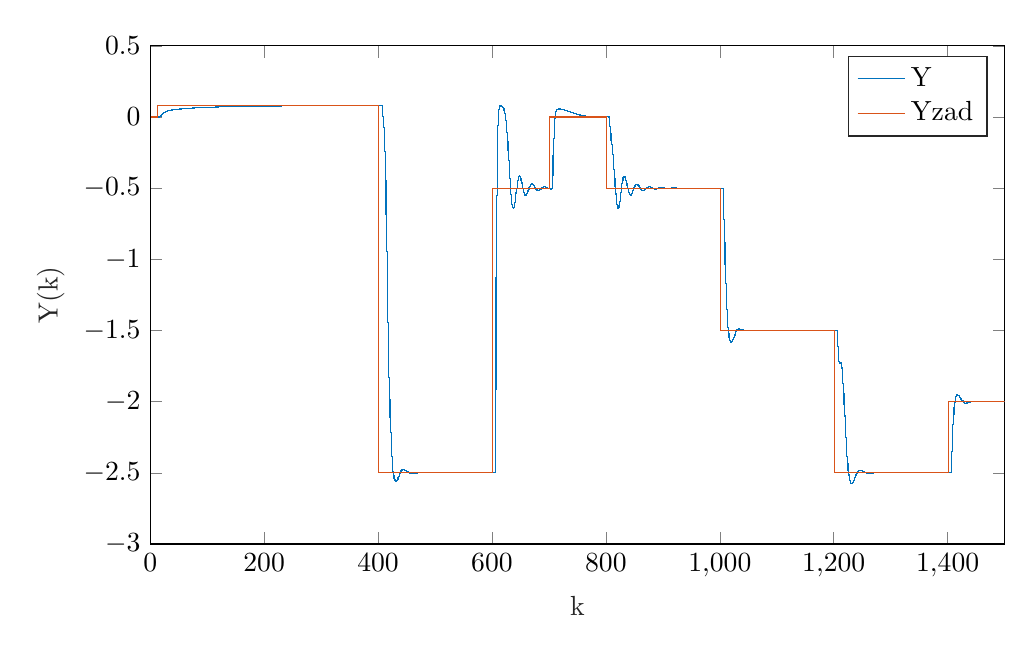
\begin{tikzpicture}

\begin{axis}[%
width=4.272in,
height=2.491in,
at={(0.717in,0.423in)},
scale only axis,
xmin=0,
xmax=1500,
xlabel style={font=\color{white!15!black}},
xlabel={k},
ymin=-3,
ymax=0.5,
ylabel style={font=\color{white!15!black}},
ylabel={Y(k)},
axis background/.style={fill=white},
legend style={legend cell align=left, align=left, draw=white!15!black}
]
\addplot[const plot, color=mycolor1] table[row sep=crcr] {%
1	0\\
2	0\\
3	0\\
4	0\\
5	0\\
6	0\\
7	0\\
8	0\\
9	0\\
10	0\\
11	0\\
12	0\\
13	0\\
14	0\\
15	0\\
16	0\\
17	0.0023297197595145\\
18	0.00708387389161341\\
19	0.0121252564854354\\
20	0.0165364802122291\\
21	0.0202080551538477\\
22	0.0233908755422572\\
23	0.0263702744785429\\
24	0.0292119158764898\\
25	0.0318403665121521\\
26	0.0341841860079102\\
27	0.0362357052533368\\
28	0.038039352483151\\
29	0.0396509370188733\\
30	0.0411099444275813\\
31	0.0424361201565352\\
32	0.0436408014569742\\
33	0.0447356271329744\\
34	0.045733449745276\\
35	0.0466470724291202\\
36	0.0474881477763321\\
37	0.048266746359285\\
38	0.0489913806382062\\
39	0.0496691984440165\\
40	0.0503061985102316\\
41	0.0509074214379866\\
42	0.051477110996899\\
43	0.0520188501963039\\
44	0.0525356759748666\\
45	0.0530301749347961\\
46	0.0535045621680834\\
47	0.0539607453974928\\
48	0.0544003768013825\\
49	0.0548248948086246\\
50	0.0552355578831425\\
51	0.0556334719744135\\
52	0.0560196129723998\\
53	0.0563948452129249\\
54	0.056759936843236\\
55	0.0571155726734573\\
56	0.0574623649988354\\
57	0.0578008627707111\\
58	0.0581315594129664\\
59	0.0584548995188697\\
60	0.0587712846159019\\
61	0.0590810781496199\\
62	0.0593846098091999\\
63	0.0596821792949996\\
64	0.0599740596108112\\
65	0.0602604999493687\\
66	0.0605417282283114\\
67	0.0608179533245902\\
68	0.061089367047774\\
69	0.0613561458865321\\
70	0.0616184525574526\\
71	0.0618764373811098\\
72	0.062130233973401\\
73	0.0623799053929322\\
74	0.0626253725092185\\
75	0.0628666131258011\\
76	0.0631036688248359\\
77	0.0633366188951918\\
78	0.0635655593522595\\
79	0.0637905914057955\\
80	0.0640118165718001\\
81	0.0642293344851812\\
82	0.0644432417542706\\
83	0.0646536313380158\\
84	0.0648605922676063\\
85	0.0650642096059463\\
86	0.0652645645570666\\
87	0.0654617346569458\\
88	0.0656557939990769\\
89	0.065846813466879\\
90	0.0660348609582697\\
91	0.0662200015958029\\
92	0.0664022979202082\\
93	0.0665818100673489\\
94	0.0667585959295672\\
95	0.0669327113027156\\
96	0.0671042100202154\\
97	0.0672731440754145\\
98	0.0674395637334056\\
99	0.067603517633347\\
100	0.0677650528822236\\
101	0.0679242151408804\\
102	0.0680810487030772\\
103	0.0682355965682329\\
104	0.0683879005084562\\
105	0.0685380011304006\\
106	0.0686859379324255\\
107	0.0688317493574929\\
108	0.0689754728421927\\
109	0.069117144862241\\
110	0.0692568009747709\\
111	0.0693944758576959\\
112	0.0695302033464032\\
113	0.0696640164680075\\
114	0.0697959474733736\\
115	0.0699260278670967\\
116	0.0700542884356103\\
117	0.0701807592735762\\
118	0.0703054698086978\\
119	0.0704284488250809\\
120	0.0705497244852605\\
121	0.0706693243509952\\
122	0.0707872754029263\\
123	0.0709036040591872\\
124	0.0710183361930422\\
125	0.0711314971496259\\
126	0.0712431117618498\\
127	0.0713532043655347\\
128	0.0714617988138242\\
129	0.0715689184909288\\
130	0.0716745863252465\\
131	0.071778824801902\\
132	0.0718816559747419\\
133	0.0719831014778225\\
134	0.0720831825364208\\
135	0.0721819199776007\\
136	0.0722793342403584\\
137	0.0723754453853766\\
138	0.0724702731044062\\
139	0.0725638367293\\
140	0.0726561552407169\\
141	0.0727472472765156\\
142	0.0728371311398534\\
143	0.0729258248070076\\
144	0.0730133459349327\\
145	0.0730997118685673\\
146	0.0731849396479035\\
147	0.0732690460148305\\
148	0.0733520474197623\\
149	0.0734339600280615\\
150	0.0735147997262668\\
151	0.0735945821281344\\
152	0.0736733225805005\\
153	0.073751036168974\\
154	0.0738277377234654\\
155	0.0739034418235591\\
156	0.0739781628037363\\
157	0.0740519147584533\\
158	0.0741247115470819\\
159	0.0741965667987165\\
160	0.074267493916854\\
161	0.0743375060839497\\
162	0.0744066162658554\\
163	0.074474837216143\\
164	0.0745421814803177\\
165	0.0746086613999253\\
166	0.0746742891165563\\
167	0.074739076575751\\
168	0.0748030355308091\\
169	0.0748661775465058\\
170	0.0749285140027186\\
171	0.0749900560979673\\
172	0.0750508148528699\\
173	0.0751108011135163\\
174	0.0751700255547642\\
175	0.0752284986834573\\
176	0.0752862308415693\\
177	0.0753432322092766\\
178	0.0753995128079604\\
179	0.0754550825031405\\
180	0.0755099510073435\\
181	0.0755641278829072\\
182	0.0756176225447216\\
183	0.0756704442629103\\
184	0.0757226021654525\\
185	0.0757741052407473\\
186	0.0758249623401229\\
187	0.0758751821802913\\
188	0.0759247733457496\\
189	0.0759737442911305\\
190	0.0760221033435024\\
191	0.0760698587046206\\
192	0.0761170184531313\\
193	0.0761635905467289\\
194	0.0762095828242682\\
195	0.0762550030078327\\
196	0.0762998587047601\\
197	0.0763441574096256\\
198	0.0763879065061848\\
199	0.0764311132692761\\
200	0.0764737848666858\\
201	0.0765159283609731\\
202	0.0765575507112604\\
203	0.0765986587749857\\
204	0.0766392593096211\\
205	0.0766793589743563\\
206	0.0767189643317483\\
207	0.0767580818493393\\
208	0.0767967179012419\\
209	0.0768348787696928\\
210	0.0768725706465768\\
211	0.0769097996349206\\
212	0.0769465717503572\\
213	0.0769828929225624\\
214	0.0770187689966632\\
215	0.0770542057346191\\
216	0.0770892088165766\\
217	0.0771237838421985\\
218	0.0771579363319671\\
219	0.0771916717284626\\
220	0.077224995397618\\
221	0.0772579126299495\\
222	0.0772904286417645\\
223	0.0773225485763457\\
224	0.0773542775051147\\
225	0.0773856204287729\\
226	0.0774165822784207\\
227	0.0774471679166576\\
228	0.0774773821386605\\
229	0.0775072296732427\\
230	0.0775367151838938\\
231	0.0775658432698\\
232	0.077594618466846\\
233	0.0776230452485992\\
234	0.0776511280272753\\
235	0.077678871154687\\
236	0.0777062789231753\\
237	0.0777333555665246\\
238	0.0777601052608606\\
239	0.0777865321255331\\
240	0.0778126402239825\\
241	0.0778384335645913\\
242	0.0778639163130624\\
243	0.0778890936999867\\
244	0.0779139718514124\\
245	0.0779385559235824\\
246	0.077962850264717\\
247	0.0779868587458873\\
248	0.0780105849739911\\
249	0.0780340323992552\\
250	0.0780572043656813\\
251	0.078080104138725\\
252	0.0781027349223604\\
253	0.0781250998698521\\
254	0.0781472020904257\\
255	0.0781690446533118\\
256	0.078190630590184\\
257	0.0782119628966623\\
258	0.0782330445332918\\
259	0.0782538784262355\\
260	0.078274467467813\\
261	0.0782948145169573\\
262	0.0783149223996274\\
263	0.0783347939091976\\
264	0.0783544318068319\\
265	0.0783738388218494\\
266	0.0783930176520846\\
267	0.0784119709642414\\
268	0.0784307013942433\\
269	0.0784492115475801\\
270	0.0784675039996498\\
271	0.0784855812960979\\
272	0.0785034459531521\\
273	0.0785211004579541\\
274	0.0785385472688878\\
275	0.0785557888159033\\
276	0.0785728275008385\\
277	0.0785896656977366\\
278	0.0786063057531602\\
279	0.0786227499865021\\
280	0.0786390006902933\\
281	0.0786550601305065\\
282	0.0786709305468578\\
283	0.0786866141531038\\
284	0.0787021131373364\\
285	0.078717429662274\\
286	0.0787325658655497\\
287	0.0787475238599962\\
288	0.0787623057339279\\
289	0.0787769135514197\\
290	0.0787913493525826\\
291	0.078805615153837\\
292	0.0788197129481822\\
293	0.0788336447054633\\
294	0.0788474123726356\\
295	0.0788610178740251\\
296	0.078874463111587\\
297	0.0788877499651614\\
298	0.0789008802927255\\
299	0.0789138559306435\\
300	0.0789266786939141\\
301	0.078939350376414\\
302	0.0789518727511407\\
303	0.0789642475704504\\
304	0.0789764765662951\\
305	0.0789885614504563\\
306	0.0790005039147756\\
307	0.0790123056313841\\
308	0.0790239682529277\\
309	0.0790354934127914\\
310	0.0790468827253198\\
311	0.0790581377860361\\
312	0.079069260171858\\
313	0.0790802514413119\\
314	0.0790911131347439\\
315	0.0791018467745291\\
316	0.0791124538652781\\
317	0.0791229358940418\\
318	0.0791332943305132\\
319	0.0791435306272273\\
320	0.079153646219759\\
321	0.079163642526918\\
322	0.0791735209509428\\
323	0.079183282877691\\
324	0.0791929296768288\\
325	0.0792024627020173\\
326	0.0792118832910978\\
327	0.0792211927662737\\
328	0.0792303924342919\\
329	0.0792394835866206\\
330	0.0792484674996263\\
331	0.0792573454347481\\
332	0.0792661186386703\\
333	0.0792747883434933\\
334	0.0792833557669018\\
335	0.079291822112332\\
336	0.0793001885691364\\
337	0.0793084563127467\\
338	0.0793166265048353\\
339	0.0793247002934742\\
340	0.079332678813293\\
341	0.0793405631856346\\
342	0.0793483545187088\\
343	0.0793560539077453\\
344	0.0793636624351435\\
345	0.0793711811706218\\
346	0.0793786111713646\\
347	0.0793859534821676\\
348	0.0793932091355818\\
349	0.0794003791520557\\
350	0.0794074645400756\\
351	0.0794144662963049\\
352	0.0794213854057209\\
353	0.0794282228417515\\
354	0.0794349795664083\\
355	0.0794416565304205\\
356	0.0794482546733651\\
357	0.0794547749237972\\
358	0.0794612181993781\\
359	0.0794675854070017\\
360	0.0794738774429205\\
361	0.0794800951928688\\
362	0.0794862395321854\\
363	0.0794923113259348\\
364	0.0794983114290266\\
365	0.0795042406863339\\
366	0.0795100999328104\\
367	0.0795158899936056\\
368	0.0795216116841794\\
369	0.0795272658104151\\
370	0.0795328531687307\\
371	0.0795383745461895\\
372	0.0795438307206093\\
373	0.0795492224606699\\
374	0.0795545505260203\\
375	0.0795598156673834\\
376	0.0795650186266607\\
377	0.0795701601370349\\
378	0.079575240923072\\
379	0.0795802617008217\\
380	0.079585223177917\\
381	0.0795901260536723\\
382	0.0795949710191808\\
383	0.0795997587574105\\
384	0.079604489943299\\
385	0.0796091652438475\\
386	0.0796137853182135\\
387	0.0796183508178026\\
388	0.079622862386359\\
389	0.0796273206600551\\
390	0.07963172626758\\
391	0.0796360798302274\\
392	0.0796403819619816\\
393	0.0796446332696033\\
394	0.0796488343527143\\
395	0.0796529858038806\\
396	0.0796570882086951\\
397	0.0796611421458596\\
398	0.0796651481872653\\
399	0.079669106898072\\
400	0.0796730188367878\\
401	0.0796768845553465\\
402	0.0796807045991846\\
403	0.0796844795073175\\
404	0.0796882098124149\\
405	0.0796918960408748\\
406	0.0832719792444984\\
407	0.0628058568568794\\
408	0.00501352782177399\\
409	-0.0441205055515054\\
410	-0.0709339676603207\\
411	-0.119738176154937\\
412	-0.243449415227726\\
413	-0.443454735025324\\
414	-0.686680146959065\\
415	-0.945710526263695\\
416	-1.201816746063\\
417	-1.44098433331021\\
418	-1.6525471706164\\
419	-1.83219283559259\\
420	-1.98217652461609\\
421	-2.10801620083529\\
422	-2.21508933678667\\
423	-2.30649392219329\\
424	-2.38339360502653\\
425	-2.44682401429643\\
426	-2.49244247697354\\
427	-2.52171752564405\\
428	-2.53960857804357\\
429	-2.55042866072333\\
430	-2.5569615175916\\
431	-2.55995379780562\\
432	-2.55901510584639\\
433	-2.55397171968747\\
434	-2.54539669343924\\
435	-2.53447634628354\\
436	-2.52264782340874\\
437	-2.51124804456541\\
438	-2.5012475792977\\
439	-2.49312881860422\\
440	-2.48695205495752\\
441	-2.48253221999942\\
442	-2.4796118583564\\
443	-2.4779610532114\\
444	-2.47740050702534\\
445	-2.47778213956922\\
446	-2.47907322112584\\
447	-2.48111582737837\\
448	-2.48364286302376\\
449	-2.48638848133776\\
450	-2.48914465077609\\
451	-2.49178992721929\\
452	-2.49426863267125\\
453	-2.49654709568088\\
454	-2.49858781246119\\
455	-2.50034694690094\\
456	-2.50178446946664\\
457	-2.5028760811428\\
458	-2.50362100423063\\
459	-2.50404318881401\\
460	-2.50418570481602\\
461	-2.50410140194076\\
462	-2.50384402566076\\
463	-2.50346253915561\\
464	-2.50299904509668\\
465	-2.50248905417092\\
466	-2.50196016570808\\
467	-2.50143744845278\\
468	-2.50094417513245\\
469	-2.50049937851572\\
470	-2.50011608282626\\
471	-2.49980061584153\\
472	-2.49955364811587\\
473	-2.49937222963834\\
474	-2.49925149851963\\
475	-2.49918557619945\\
476	-2.49916783200527\\
477	-2.49919090916428\\
478	-2.49924681012395\\
479	-2.49932717001451\\
480	-2.49942371110588\\
481	-2.49952875771076\\
482	-2.49963566066686\\
483	-2.49973903474495\\
484	-2.49983480017889\\
485	-2.49992008588039\\
486	-2.49999312041636\\
487	-2.50005297486531\\
488	-2.50009938945232\\
489	-2.50013269765658\\
490	-2.50015375937609\\
491	-2.50016387156194\\
492	-2.50016463494947\\
493	-2.50015779682293\\
494	-2.50014511241722\\
495	-2.50012824841513\\
496	-2.5001087277061\\
497	-2.50008790158219\\
498	-2.50006693504749\\
499	-2.50004679675576\\
500	-2.50002825137214\\
501	-2.50001185678349\\
502	-2.49999796984782\\
503	-2.49998676253247\\
504	-2.49997824718658\\
505	-2.4999723073125\\
506	-2.49996872853049\\
507	-2.49996723041235\\
508	-2.49996749361\\
509	-2.49996918080039\\
510	-2.49997195336185\\
511	-2.49997548518612\\
512	-2.49997947462412\\
513	-2.49998365436937\\
514	-2.4999877983107\\
515	-2.49999172480862\\
516	-2.49999529666427\\
517	-2.49999841862118\\
518	-2.50000103335827\\
519	-2.5000031167248\\
520	-2.50000467266757\\
521	-2.50000572805292\\
522	-2.50000632747027\\
523	-2.50000652811177\\
524	-2.50000639488643\\
525	-2.50000599597318\\
526	-2.5000053990265\\
527	-2.50000466807522\\
528	-2.50000386121665\\
529	-2.50000302909994\\
530	-2.50000221407849\\
531	-2.50000144989585\\
532	-2.50000076178082\\
533	-2.50000016686587\\
534	-2.49999967487604\\
535	-2.49999928903592\\
536	-2.49999900712602\\
537	-2.4999988226084\\
538	-2.4999987257442\\
539	-2.49999870464237\\
540	-2.49999874620009\\
541	-2.49999883691471\\
542	-2.4999989635604\\
543	-2.49999911372947\\
544	-2.49999927624148\\
545	-2.49999944142531\\
546	-2.4999996012818\\
547	-2.49999974954083\\
548	-2.49999988162721\\
549	-2.49999999455311\\
550	-2.50000008675643\\
551	-2.50000015790448\\
552	-2.50000020867953\\
553	-2.50000024055986\\
554	-2.50000025560605\\
555	-2.50000025626053\\
556	-2.50000024516616\\
557	-2.50000022500871\\
558	-2.50000019838645\\
559	-2.50000016770795\\
560	-2.50000013511799\\
561	-2.50000010244949\\
562	-2.50000007119856\\
563	-2.50000004251947\\
564	-2.50000001723584\\
565	-2.49999999586456\\
566	-2.49999997864911\\
567	-2.49999996559913\\
568	-2.49999995653334\\
569	-2.49999995112316\\
570	-2.49999994893514\\
571	-2.49999994947013\\
572	-2.4999999521982\\
573	-2.4999999565884\\
574	-2.49999996213297\\
575	-2.49999996836605\\
576	-2.499999974877\\
577	-2.49999998131881\\
578	-2.49999998741202\\
579	-2.49999999294491\\
580	-2.4999999977705\\
581	-2.50000000180121\\
582	-2.50000000500178\\
583	-2.50000000738116\\
584	-2.50000000898388\\
585	-2.50000000988142\\
586	-2.500000010164\\
587	-2.50000000993296\\
588	-2.50000000929415\\
589	-2.50000000835228\\
590	-2.50000000720636\\
591	-2.50000000594627\\
592	-2.50000000465038\\
593	-2.50000000338413\\
594	-2.50000000219947\\
595	-2.50000000113498\\
596	-2.50000000021666\\
597	-2.49999999945903\\
598	-2.49999999886661\\
599	-2.49999999843562\\
600	-2.49999999815563\\
601	-2.49999999801131\\
602	-2.49999999798401\\
603	-2.49999999805325\\
604	-2.49999999819795\\
605	-2.49999999839754\\
606	-1.9169241234065\\
607	-1.12692809942908\\
608	-0.549849515787396\\
609	-0.226719461562416\\
610	-0.0622519795443552\\
611	0.0174050608454842\\
612	0.0551826906696555\\
613	0.0728261092402602\\
614	0.0802068229490298\\
615	0.0815894175435637\\
616	0.0795304071896676\\
617	0.0756900042494271\\
618	0.0710142618378024\\
619	0.065597617675508\\
620	0.0579326185300353\\
621	0.044938601133809\\
622	0.0263816255510117\\
623	0.00346762987017489\\
624	-0.0250956620023283\\
625	-0.0627850821835598\\
626	-0.111731101730157\\
627	-0.170547368112402\\
628	-0.235539042279308\\
629	-0.302868986736689\\
630	-0.36962652726923\\
631	-0.43354303404844\\
632	-0.492425996435975\\
633	-0.544067166010521\\
634	-0.586395170482418\\
635	-0.617679299203822\\
636	-0.636769368436073\\
637	-0.64333629928319\\
638	-0.637984136916042\\
639	-0.62213527812132\\
640	-0.597797461277122\\
641	-0.567398697466603\\
642	-0.533787518763486\\
643	-0.500103588927373\\
644	-0.469375035833471\\
645	-0.444090068755518\\
646	-0.425932894745462\\
647	-0.415714177023117\\
648	-0.413438836167273\\
649	-0.4184452755615\\
650	-0.429534944385812\\
651	-0.445149505928674\\
652	-0.463554121401259\\
653	-0.482998182808449\\
654	-0.501848339247363\\
655	-0.518694176724502\\
656	-0.532424349346579\\
657	-0.542271721962864\\
658	-0.547830795233993\\
659	-0.549052545740683\\
660	-0.546220040905277\\
661	-0.539905748614763\\
662	-0.530911095615171\\
663	-0.520190738762303\\
664	-0.508766594416491\\
665	-0.497638664100823\\
666	-0.487700910943298\\
667	-0.479670638299894\\
668	-0.474039105936661\\
669	-0.471048144775882\\
670	-0.470693369665107\\
671	-0.47275047737915\\
672	-0.476818410213934\\
673	-0.482372382767464\\
674	-0.4888203972688\\
675	-0.495558063137784\\
676	-0.502017744166887\\
677	-0.50770916315145\\
678	-0.512249646698667\\
679	-0.515383176040918\\
680	-0.516988246989562\\
681	-0.51707517338592\\
682	-0.515773921696289\\
683	-0.513313942355268\\
684	-0.509997850738645\\
685	-0.506171204506845\\
686	-0.502190935213973\\
687	-0.498395120496712\\
688	-0.495076610598379\\
689	-0.492462593083146\\
690	-0.490701506318309\\
691	-0.4898578922851\\
692	-0.489914938465428\\
693	-0.490783715172009\\
694	-0.492317566707347\\
695	-0.494329815975638\\
696	-0.49661289076741\\
697	-0.498957127677581\\
698	-0.50116778730677\\
699	-0.50307915732859\\
700	-0.504564981461639\\
701	-0.505544804818802\\
702	-0.505986154942017\\
703	-0.505902774609603\\
704	-0.505349380658102\\
705	-0.504413635618452\\
706	-0.40794252399511\\
707	-0.272885521570123\\
708	-0.152570585366441\\
709	-0.0657607735789843\\
710	-0.0115129472369605\\
711	0.0195581321055302\\
712	0.0371576046857302\\
713	0.0471311614339347\\
714	0.0526692858966331\\
715	0.055535028214404\\
716	0.0567750388842225\\
717	0.0570471312121187\\
718	0.0567644250055596\\
719	0.0561766761238194\\
720	0.0554264509369789\\
721	0.0545895357507973\\
722	0.0537026558525755\\
723	0.0527811512190427\\
724	0.0518294232430233\\
725	0.0508466706486009\\
726	0.0498298250750872\\
727	0.0487749595230766\\
728	0.047677932863624\\
729	0.0465346865551481\\
730	0.0453414016220128\\
731	0.0440946106070804\\
732	0.0427927305439984\\
733	0.0414414523508903\\
734	0.0400507536895607\\
735	0.0386302655991366\\
736	0.0371877591452122\\
737	0.0357291484555976\\
738	0.0342595126671231\\
739	0.0327843202513031\\
740	0.031309982543336\\
741	0.0298434174898285\\
742	0.0283910856407416\\
743	0.0269583242583584\\
744	0.025549448792426\\
745	0.0241684062220049\\
746	0.0228193595925793\\
747	0.0215067333078912\\
748	0.020234739717199\\
749	0.0190067990447043\\
750	0.017825277424902\\
751	0.0166916593205141\\
752	0.0156069398978511\\
753	0.0145719221668637\\
754	0.0135872492817757\\
755	0.0126532333415108\\
756	0.0117696733172205\\
757	0.0109358170416053\\
758	0.0101504852433207\\
759	0.00941226082616858\\
760	0.0087196277935482\\
761	0.00807100872872398\\
762	0.00746473066230656\\
763	0.00689898694968206\\
764	0.00637184408623287\\
765	0.00588129602926889\\
766	0.0054253338496911\\
767	0.00500199540635803\\
768	0.00460938108477316\\
769	0.00424564603973836\\
770	0.00390898974324947\\
771	0.00359765733631824\\
772	0.00330995353330758\\
773	0.00304425997302876\\
774	0.00279904624471106\\
775	0.00257287093799549\\
776	0.00236437584572514\\
777	0.00217227922367386\\
778	0.0019953721978598\\
779	0.00183251861313209\\
780	0.00168265592319697\\
781	0.0015447945278755\\
782	0.00141801459307696\\
783	0.00130146119248145\\
784	0.0011943393480325\\
785	0.00109591006837869\\
786	0.00100548748004655\\
787	0.000922436428544992\\
788	0.000846169863961558\\
789	0.000776145743936653\\
790	0.000711863656589616\\
791	0.000652861562578328\\
792	0.000598712936412789\\
793	0.000549024328646527\\
794	0.000503433182974342\\
795	0.000461605722643261\\
796	0.000423234826290596\\
797	0.000388037934615496\\
798	0.000355755081983521\\
799	0.000326147118727598\\
800	0.000298994124694583\\
801	0.000274093966345242\\
802	0.000251260944005283\\
803	0.000230324502558971\\
804	0.000211128010244011\\
805	0.00019352762452548\\
806	-0.0196863475092192\\
807	-0.0661785268100687\\
808	-0.118799080808691\\
809	-0.163457965879903\\
810	-0.195669212228537\\
811	-0.224606189688643\\
812	-0.261648400963294\\
813	-0.311214535749955\\
814	-0.370082803462756\\
815	-0.431663300834624\\
816	-0.489900665899103\\
817	-0.540839228554732\\
818	-0.582343828927517\\
819	-0.613213214213744\\
820	-0.632594713914509\\
821	-0.639924233311294\\
822	-0.635234545577436\\
823	-0.619529615907536\\
824	-0.594914707168599\\
825	-0.564329146149796\\
826	-0.531091779789087\\
827	-0.498401517882799\\
828	-0.468977886466978\\
829	-0.444937079450475\\
830	-0.427740612138754\\
831	-0.41814710430142\\
832	-0.416204688024192\\
833	-0.421304003645626\\
834	-0.432268835168768\\
835	-0.447556970669236\\
836	-0.465475719183106\\
837	-0.484344980797039\\
838	-0.502607142786899\\
839	-0.51890916254743\\
840	-0.532170700006419\\
841	-0.541635872293135\\
842	-0.546902234894233\\
843	-0.547923380136502\\
844	-0.54498588385188\\
845	-0.538664007924185\\
846	-0.529757536186251\\
847	-0.519211134736662\\
848	-0.50802862607143\\
849	-0.497185689397192\\
850	-0.487548162449689\\
851	-0.47980504219285\\
852	-0.474423155455623\\
853	-0.471626659244201\\
854	-0.471400938333139\\
855	-0.473517978317441\\
856	-0.477578383264189\\
857	-0.48306380459066\\
858	-0.489393087600739\\
859	-0.495976241257646\\
860	-0.502262007506739\\
861	-0.50777654182964\\
862	-0.512151973093991\\
863	-0.515144350921983\\
864	-0.516640968904662\\
865	-0.516657501764652\\
866	-0.51532584522386\\
867	-0.512874211311888\\
868	-0.509601152459527\\
869	-0.505845802830631\\
870	-0.501956930135305\\
871	-0.498263438404498\\
872	-0.495048808741774\\
873	-0.492531492355937\\
874	-0.490852566750868\\
875	-0.490071145045661\\
876	-0.490167216475053\\
877	-0.491050912140721\\
878	-0.492576702814162\\
879	-0.49456076564827\\
880	-0.496799695685737\\
881	-0.499088859144786\\
882	-0.501238944705878\\
883	-0.503089610652845\\
884	-0.504519494772717\\
885	-0.505452210034665\\
886	-0.505858272749521\\
887	-0.505753190844105\\
888	-0.50519219125396\\
889	-0.504262264571416\\
890	-0.503072355224371\\
891	-0.501742616047171\\
892	-0.50039366395521\\
893	-0.499136715959794\\
894	-0.498065353545496\\
895	-0.497249470195175\\
896	-0.49673172320495\\
897	-0.496526563726057\\
898	-0.496621685919696\\
899	-0.496981540860066\\
900	-0.49755241932496\\
901	-0.498268526975104\\
902	-0.499058454735731\\
903	-0.49985147952731\\
904	-0.500583205181757\\
905	-0.501200158058496\\
906	-0.501663074058278\\
907	-0.501948742086045\\
908	-0.502050393513953\\
909	-0.50197674026459\\
910	-0.501749859372585\\
911	-0.501402194471908\\
912	-0.500972991288797\\
913	-0.500504503011095\\
914	-0.500038292383549\\
915	-0.499611922655245\\
916	-0.499256273270161\\
917	-0.49899364448696\\
918	-0.498836735239611\\
919	-0.498788498245627\\
920	-0.498842802912571\\
921	-0.498985775985425\\
922	-0.499197646259592\\
923	-0.499454895092172\\
924	-0.499732508878733\\
925	-0.500006141411594\\
926	-0.500254020130215\\
927	-0.50045846697429\\
928	-0.500606947793123\\
929	-0.500692610005738\\
930	-0.500714312707173\\
931	-0.500676193432672\\
932	-0.500586848707093\\
933	-0.500458229437066\\
934	-0.500304366054716\\
935	-0.500140041822193\\
936	-0.499979526392709\\
937	-0.499835466872699\\
938	-0.49971801212842\\
939	-0.499634220242463\\
940	-0.499587771366007\\
941	-0.49957898120755\\
942	-0.499605086260329\\
943	-0.499660752363045\\
944	-0.499738744505746\\
945	-0.499830688507336\\
946	-0.499927854271222\\
947	-0.500021895208681\\
948	-0.500105488125499\\
949	-0.500172831131775\\
950	-0.500219972544565\\
951	-0.500244959874125\\
952	-0.500247813472536\\
953	-0.500230343113267\\
954	-0.500195836744023\\
955	-0.500148658287761\\
956	-0.500093795346973\\
957	-0.500036397996872\\
958	-0.499981346826397\\
959	-0.499932882540108\\
960	-0.49989432149149\\
961	-0.499867872312423\\
962	-0.499854559200835\\
963	-0.499854248252149\\
964	-0.499865765183869\\
965	-0.499887086460275\\
966	-0.499915581536644\\
967	-0.499948281866593\\
968	-0.499982152411623\\
969	-0.500014343444509\\
970	-0.500042404095708\\
971	-0.500064443906554\\
972	-0.500079234127629\\
973	-0.500086246132979\\
974	-0.50008562964368\\
975	-0.500078138068923\\
976	-0.500065011873786\\
977	-0.500047833273295\\
978	-0.500028366649997\\
979	-0.500008398925767\\
980	-0.499989592815802\\
981	-0.499973363662143\\
982	-0.499960787650595\\
983	-0.499952545953768\\
984	-0.499948906012891\\
985	-0.49994973804907\\
986	-0.499954562215597\\
987	-0.499962619743768\\
988	-0.499972960105136\\
989	-0.499984535653505\\
990	-0.499996295393818\\
991	-0.500007270368261\\
992	-0.500016644522649\\
993	-0.500023806658212\\
994	-0.500028381010063\\
995	-0.500030235949627\\
996	-0.500029472124353\\
997	-0.500026392890403\\
998	-0.500021461063497\\
999	-0.500015246749368\\
1000	-0.500008371298746\\
1001	-0.500001452280901\\
1002	-0.499995053836677\\
1003	-0.499989645934739\\
1004	-0.49998557500917\\
1005	-0.499983047306487\\
1006	-0.573080495533453\\
1007	-0.717286004687272\\
1008	-0.882697286349006\\
1009	-1.03762995702672\\
1010	-1.16723397514686\\
1011	-1.27125836243978\\
1012	-1.35499730263221\\
1013	-1.4229203806225\\
1014	-1.47743829290207\\
1015	-1.51963624362563\\
1016	-1.55029566413024\\
1017	-1.57048704289928\\
1018	-1.58168312598847\\
1019	-1.58560850322116\\
1020	-1.58402603954675\\
1021	-1.57856845006357\\
1022	-1.5706425624036\\
1023	-1.56139350219121\\
1024	-1.55170699960412\\
1025	-1.54223222712642\\
1026	-1.53133242190178\\
1027	-1.51967742092016\\
1028	-1.50901174691669\\
1029	-1.50053902477553\\
1030	-1.49468927601021\\
1031	-1.49120001065881\\
1032	-1.4894870938457\\
1033	-1.48897282697159\\
1034	-1.48922525348932\\
1035	-1.48996541842508\\
1036	-1.49101770252425\\
1037	-1.49225899828756\\
1038	-1.49358928087927\\
1039	-1.49492221091294\\
1040	-1.49618630838513\\
1041	-1.49732835270901\\
1042	-1.49831477119943\\
1043	-1.49913021259195\\
1044	-1.49977419128127\\
1045	-1.50025702029477\\
1046	-1.50063931791257\\
1047	-1.50093874158459\\
1048	-1.50113711958181\\
1049	-1.5012197876093\\
1050	-1.5011912008177\\
1051	-1.50107670377804\\
1052	-1.50091170295753\\
1053	-1.50072900513681\\
1054	-1.5005518761474\\
1055	-1.50039311063385\\
1056	-1.50025764797124\\
1057	-1.5001459864508\\
1058	-1.50005675353762\\
1059	-1.49998804402501\\
1060	-1.49993784521827\\
1061	-1.49990403651787\\
1062	-1.49988431854502\\
1063	-1.49987622572154\\
1064	-1.49987723208421\\
1065	-1.49988489910456\\
1066	-1.49989609057879\\
1067	-1.4999088846143\\
1068	-1.499922737147\\
1069	-1.4999375221453\\
1070	-1.49995287556603\\
1071	-1.49996796998786\\
1072	-1.49998174993692\\
1073	-1.49999332512281\\
1074	-1.50000222520532\\
1075	-1.50000843480962\\
1076	-1.50001226921074\\
1077	-1.50001419928789\\
1078	-1.50001470903471\\
1079	-1.50001421719674\\
1080	-1.50001305499408\\
1081	-1.50001147570238\\
1082	-1.50000967379279\\
1083	-1.50000780090765\\
1084	-1.50000597505717\\
1085	-1.50000428464636\\
1086	-1.50000280995927\\
1087	-1.50000158866363\\
1088	-1.50000060988919\\
1089	-1.4999998399081\\
1090	-1.49999924682099\\
1091	-1.49999881318877\\
1092	-1.49999853286854\\
1093	-1.49999839976782\\
1094	-1.49999839882416\\
1095	-1.49999850396018\\
1096	-1.49999868217546\\
1097	-1.49999890008553\\
1098	-1.49999912939802\\
1099	-1.49999934962746\\
1100	-1.49999954814677\\
1101	-1.49999971863305\\
1102	-1.4999998590569\\
1103	-1.4999999699675\\
1104	-1.50000005334343\\
1105	-1.50000011194759\\
1106	-1.50000014857941\\
1107	-1.50000016661287\\
1108	-1.50000017016363\\
1109	-1.50000016346994\\
1110	-1.50000015016043\\
1111	-1.50000013283414\\
1112	-1.50000011314317\\
1113	-1.50000009219972\\
1114	-1.50000007097595\\
1115	-1.50000005048823\\
1116	-1.50000003174984\\
1117	-1.50000001560523\\
1118	-1.50000000257969\\
1119	-1.49999999282329\\
1120	-1.4999999861561\\
1121	-1.49999998217519\\
1122	-1.49999998037333\\
1123	-1.49999998023382\\
1124	-1.49999998128797\\
1125	-1.49999998313904\\
1126	-1.49999998547346\\
1127	-1.49999998803871\\
1128	-1.49999999062405\\
1129	-1.49999999306179\\
1130	-1.49999999523681\\
1131	-1.49999999709083\\
1132	-1.49999999861353\\
1133	-1.49999999982382\\
1134	-1.50000000075085\\
1135	-1.50000000142254\\
1136	-1.50000000186323\\
1137	-1.50000000209715\\
1138	-1.50000000215271\\
1139	-1.50000000206423\\
1140	-1.50000000187021\\
1141	-1.5000000016095\\
1142	-1.50000000131717\\
1143	-1.50000000102156\\
1144	-1.50000000074315\\
1145	-1.50000000049496\\
1146	-1.50000000028368\\
1147	-1.50000000011156\\
1148	-1.49999999997812\\
1149	-1.4999999998811\\
1150	-1.49999999981682\\
1151	-1.49999999978047\\
1152	-1.49999999976649\\
1153	-1.49999999976929\\
1154	-1.49999999978385\\
1155	-1.49999999980612\\
1156	-1.499999999833\\
1157	-1.49999999986217\\
1158	-1.4999999998918\\
1159	-1.4999999999204\\
1160	-1.49999999994667\\
1161	-1.49999999996965\\
1162	-1.49999999998871\\
1163	-1.50000000000358\\
1164	-1.50000000001436\\
1165	-1.50000000002144\\
1166	-1.50000000002535\\
1167	-1.50000000002672\\
1168	-1.50000000002616\\
1169	-1.50000000002421\\
1170	-1.50000000002135\\
1171	-1.50000000001798\\
1172	-1.50000000001445\\
1173	-1.50000000001101\\
1174	-1.50000000000786\\
1175	-1.50000000000509\\
1176	-1.50000000000277\\
1177	-1.5000000000009\\
1178	-1.49999999999945\\
1179	-1.49999999999838\\
1180	-1.49999999999767\\
1181	-1.49999999999725\\
1182	-1.4999999999971\\
1183	-1.49999999999715\\
1184	-1.49999999999736\\
1185	-1.49999999999767\\
1186	-1.49999999999804\\
1187	-1.49999999999843\\
1188	-1.49999999999882\\
1189	-1.49999999999917\\
1190	-1.49999999999948\\
1191	-1.49999999999974\\
1192	-1.49999999999995\\
1193	-1.5000000000001\\
1194	-1.50000000000021\\
1195	-1.50000000000028\\
1196	-1.50000000000031\\
1197	-1.50000000000032\\
1198	-1.50000000000031\\
1199	-1.50000000000028\\
1200	-1.50000000000024\\
1201	-1.5000000000002\\
1202	-1.50000000000016\\
1203	-1.50000000000012\\
1204	-1.50000000000009\\
1205	-1.50000000000005\\
1206	-1.54222913660834\\
1207	-1.61326328503289\\
1208	-1.67840877504907\\
1209	-1.71939630711625\\
1210	-1.73243573079221\\
1211	-1.72916997481365\\
1212	-1.72620307167179\\
1213	-1.73572324781671\\
1214	-1.76333469665091\\
1215	-1.80930898660811\\
1216	-1.87059017400418\\
1217	-1.94261899785901\\
1218	-2.02066411952328\\
1219	-2.1005737127342\\
1220	-2.17904107621842\\
1221	-2.25357665530003\\
1222	-2.32210892100679\\
1223	-2.38325867642907\\
1224	-2.43630853776187\\
1225	-2.48093594282264\\
1226	-2.51510887917041\\
1227	-2.53934852246022\\
1228	-2.55571235001903\\
1229	-2.56610236331821\\
1230	-2.57189229645183\\
1231	-2.57381755892373\\
1232	-2.57225576997925\\
1233	-2.56758846447441\\
1234	-2.56037256296678\\
1235	-2.55133237292203\\
1236	-2.54126075177235\\
1237	-2.53090774014101\\
1238	-2.52090129475942\\
1239	-2.5117121411531\\
1240	-2.50365438079603\\
1241	-2.49690633655689\\
1242	-2.49153799653247\\
1243	-2.4875368961373\\
1244	-2.48482946361204\\
1245	-2.48329800775829\\
1246	-2.48283767033498\\
1247	-2.48328031626665\\
1248	-2.48441177804805\\
1249	-2.48602151325639\\
1250	-2.48792777431344\\
1251	-2.48998835944004\\
1252	-2.4920948860586\\
1253	-2.49416055821777\\
1254	-2.49611200005891\\
1255	-2.49788730405022\\
1256	-2.49943802452645\\
1257	-2.50073188318628\\
1258	-2.50175394688926\\
1259	-2.50250560310243\\
1260	-2.50300180034276\\
1261	-2.50326746662652\\
1262	-2.50333392741772\\
1263	-2.50323581376716\\
1264	-2.5030086240897\\
1265	-2.5026868966814\\
1266	-2.50230195638987\\
1267	-2.50188274245443\\
1268	-2.5014553342972\\
1269	-2.50104162603433\\
1270	-2.50065853564516\\
1271	-2.50031783461145\\
1272	-2.5000266674031\\
1273	-2.49978844187489\\
1274	-2.49960368350945\\
1275	-2.49947067967664\\
1276	-2.49938593315931\\
1277	-2.49934452701945\\
1278	-2.49934049001456\\
1279	-2.49936719418614\\
1280	-2.49941776509969\\
1281	-2.49948546286679\\
1282	-2.49956399652058\\
1283	-2.49964775239351\\
1284	-2.49973193590032\\
1285	-2.49981263838162\\
1286	-2.49988686470628\\
1287	-2.49995246228507\\
1288	-2.50000804480077\\
1289	-2.50005292554377\\
1290	-2.50008703629875\\
1291	-2.50011082774444\\
1292	-2.50012515174053\\
1293	-2.50013113751949\\
1294	-2.50013007783116\\
1295	-2.50012333446499\\
1296	-2.50011226470028\\
1297	-2.5000981653772\\
1298	-2.50008223030263\\
1299	-2.50006551819617\\
1300	-2.50004893024724\\
1301	-2.50003319733401\\
1302	-2.50001887684951\\
1303	-2.50000635834739\\
1304	-2.49999587643787\\
1305	-2.4999875289084\\
1306	-2.49998129758409\\
1307	-2.49997707165909\\
1308	-2.49997467057413\\
1309	-2.49997386497523\\
1310	-2.49997439567192\\
1311	-2.49997599050953\\
1312	-2.49997837907678\\
1313	-2.49998130494757\\
1314	-2.49998453508652\\
1315	-2.4999878662865\\
1316	-2.49999112882958\\
1317	-2.49999418779784\\
1318	-2.49999694254007\\
1319	-2.49999932475601\\
1320	-2.5000012955678\\
1321	-2.50000284187106\\
1322	-2.50000397221678\\
1323	-2.50000471245955\\
1324	-2.50000510139726\\
1325	-2.50000518660523\\
1326	-2.50000502063986\\
1327	-2.50000465769849\\
1328	-2.5000041508322\\
1329	-2.50000354975233\\
1330	-2.50000289920983\\
1331	-2.50000223790096\\
1332	-2.50000159784027\\
1333	-2.50000100414132\\
1334	-2.50000047514714\\
1335	-2.50000002284766\\
1336	-2.49999965351534\\
1337	-2.49999936848788\\
1338	-2.49999916503077\\
1339	-2.49999903722199\\
1340	-2.49999897681339\\
1341	-2.49999897403472\\
1342	-2.49999901831653\\
1343	-2.49999909891569\\
1344	-2.499999205434\\
1345	-2.49999932822612\\
1346	-2.49999945869801\\
1347	-2.4999995895028\\
1348	-2.49999971464337\\
1349	-2.49999982949394\\
1350	-2.49999993075487\\
1351	-2.50000001635554\\
1352	-2.5000000853199\\
1353	-2.50000013760762\\
1354	-2.50000017394256\\
1355	-2.50000019563824\\
1356	-2.50000020442886\\
1357	-2.50000020231228\\
1358	-2.50000019141022\\
1359	-2.5000001738488\\
1360	-2.50000015166127\\
1361	-2.50000012671307\\
1362	-2.50000010064847\\
1363	-2.50000007485713\\
1364	-2.50000005045838\\
1365	-2.50000002830061\\
1366	-2.50000000897307\\
1367	-2.49999999282717\\
1368	-2.49999998000471\\
1369	-2.49999997047035\\
1370	-2.4999999640461\\
1371	-2.49999996044592\\
1372	-2.49999995930877\\
1373	-2.49999996022891\\
1374	-2.49999996278261\\
1375	-2.49999996655068\\
1376	-2.49999997113669\\
1377	-2.49999997618066\\
1378	-2.49999998136872\\
1379	-2.49999998643872\\
1380	-2.49999999118257\\
1381	-2.4999999954456\\
1382	-2.4999999991237\\
1383	-2.5000000021586\\
1384	-2.50000000453205\\
1385	-2.50000000625918\\
1386	-2.50000000738165\\
1387	-2.50000000796079\\
1388	-2.50000000807123\\
1389	-2.50000000779496\\
1390	-2.50000000721635\\
1391	-2.50000000641776\\
1392	-2.5000000054763\\
1393	-2.50000000446118\\
1394	-2.50000000343216\\
1395	-2.50000000243849\\
1396	-2.50000000151869\\
1397	-2.50000000070078\\
1398	-2.50000000000295\\
1399	-2.49999999943455\\
1400	-2.49999999899736\\
1401	-2.49999999868683\\
1402	-2.49999999849354\\
1403	-2.49999999840449\\
1404	-2.49999999840436\\
1405	-2.49999999847665\\
1406	-2.44278286051698\\
1407	-2.34863392123394\\
1408	-2.249613426512\\
1409	-2.16214812361625\\
1410	-2.09215446567747\\
1411	-2.04002119471735\\
1412	-2.0034490565615\\
1413	-1.97921191998834\\
1414	-1.96421721814955\\
1415	-1.95595061430228\\
1416	-1.95252626504335\\
1417	-1.95256335531753\\
1418	-1.9550325510752\\
1419	-1.9591378803149\\
1420	-1.96424575948451\\
1421	-1.96984878152809\\
1422	-1.97554788961488\\
1423	-1.98104114044988\\
1424	-1.98611314069201\\
1425	-1.99062340417959\\
1426	-1.99551025513364\\
1427	-2.00059352567388\\
1428	-2.00511091217808\\
1429	-2.00851696348458\\
1430	-2.01061855262297\\
1431	-2.01151308974655\\
1432	-2.01145623519299\\
1433	-2.01074009437992\\
1434	-2.00962040303827\\
1435	-2.00829036769032\\
1436	-2.0068837351709\\
1437	-2.00548951734156\\
1438	-2.00416700400451\\
1439	-2.00295634356405\\
1440	-2.00188439047623\\
1441	-2.00096740779831\\
1442	-2.0002123749417\\
1443	-1.99961805797553\\
1444	-1.99917632594854\\
1445	-1.998873741474\\
1446	-1.99867153736264\\
1447	-1.99855178688775\\
1448	-1.99851468184596\\
1449	-1.99855933839124\\
1450	-1.99867613277457\\
1451	-1.99884664768887\\
1452	-1.99904826594038\\
1453	-1.99925950648395\\
1454	-1.99946346418814\\
1455	-1.99964888308307\\
1456	-1.99980954796702\\
1457	-1.99994295904424\\
1458	-2.00004901449244\\
1459	-2.00012903692764\\
1460	-2.00018517877146\\
1461	-2.00022009624343\\
1462	-2.00023676040559\\
1463	-2.00023831409329\\
1464	-2.00022793477227\\
1465	-2.00020869941081\\
1466	-2.00018392448137\\
1467	-2.00015617162136\\
1468	-2.00012711221361\\
1469	-2.00009797156692\\
1470	-2.00006984514151\\
1471	-2.00004380046007\\
1472	-2.00002079239087\\
1473	-2.00000151662008\\
1474	-1.99998631637357\\
1475	-1.99997518122563\\
1476	-1.99996781878248\\
1477	-1.9999637569672\\
1478	-1.99996243996148\\
1479	-1.99996329870164\\
1480	-1.99996579339543\\
1481	-1.9999694347727\\
1482	-1.99997379286659\\
1483	-1.99997850002742\\
1484	-1.99998325166587\\
1485	-1.99998780574783\\
1486	-1.99999197106563\\
1487	-1.99999562161848\\
1488	-1.999998695942\\
1489	-2.00000117963792\\
1490	-2.00000308748439\\
1491	-2.00000445142669\\
1492	-2.00000531579575\\
1493	-2.00000573656387\\
1494	-2.00000578047282\\
1495	-2.00000552195877\\
1496	-2.00000503809477\\
1497	-2.00000440300732\\
1498	-2.0000036832484\\
1499	-2.00000293492404\\
1500	-2.00000220261746\\
};
\addlegendentry{Y}

\addplot[const plot, color=mycolor2] table[row sep=crcr] {%
1	0\\
2	0\\
3	0\\
4	0\\
5	0\\
6	0\\
7	0\\
8	0\\
9	0\\
10	0\\
11	0\\
12	0.08\\
13	0.08\\
14	0.08\\
15	0.08\\
16	0.08\\
17	0.08\\
18	0.08\\
19	0.08\\
20	0.08\\
21	0.08\\
22	0.08\\
23	0.08\\
24	0.08\\
25	0.08\\
26	0.08\\
27	0.08\\
28	0.08\\
29	0.08\\
30	0.08\\
31	0.08\\
32	0.08\\
33	0.08\\
34	0.08\\
35	0.08\\
36	0.08\\
37	0.08\\
38	0.08\\
39	0.08\\
40	0.08\\
41	0.08\\
42	0.08\\
43	0.08\\
44	0.08\\
45	0.08\\
46	0.08\\
47	0.08\\
48	0.08\\
49	0.08\\
50	0.08\\
51	0.08\\
52	0.08\\
53	0.08\\
54	0.08\\
55	0.08\\
56	0.08\\
57	0.08\\
58	0.08\\
59	0.08\\
60	0.08\\
61	0.08\\
62	0.08\\
63	0.08\\
64	0.08\\
65	0.08\\
66	0.08\\
67	0.08\\
68	0.08\\
69	0.08\\
70	0.08\\
71	0.08\\
72	0.08\\
73	0.08\\
74	0.08\\
75	0.08\\
76	0.08\\
77	0.08\\
78	0.08\\
79	0.08\\
80	0.08\\
81	0.08\\
82	0.08\\
83	0.08\\
84	0.08\\
85	0.08\\
86	0.08\\
87	0.08\\
88	0.08\\
89	0.08\\
90	0.08\\
91	0.08\\
92	0.08\\
93	0.08\\
94	0.08\\
95	0.08\\
96	0.08\\
97	0.08\\
98	0.08\\
99	0.08\\
100	0.08\\
101	0.08\\
102	0.08\\
103	0.08\\
104	0.08\\
105	0.08\\
106	0.08\\
107	0.08\\
108	0.08\\
109	0.08\\
110	0.08\\
111	0.08\\
112	0.08\\
113	0.08\\
114	0.08\\
115	0.08\\
116	0.08\\
117	0.08\\
118	0.08\\
119	0.08\\
120	0.08\\
121	0.08\\
122	0.08\\
123	0.08\\
124	0.08\\
125	0.08\\
126	0.08\\
127	0.08\\
128	0.08\\
129	0.08\\
130	0.08\\
131	0.08\\
132	0.08\\
133	0.08\\
134	0.08\\
135	0.08\\
136	0.08\\
137	0.08\\
138	0.08\\
139	0.08\\
140	0.08\\
141	0.08\\
142	0.08\\
143	0.08\\
144	0.08\\
145	0.08\\
146	0.08\\
147	0.08\\
148	0.08\\
149	0.08\\
150	0.08\\
151	0.08\\
152	0.08\\
153	0.08\\
154	0.08\\
155	0.08\\
156	0.08\\
157	0.08\\
158	0.08\\
159	0.08\\
160	0.08\\
161	0.08\\
162	0.08\\
163	0.08\\
164	0.08\\
165	0.08\\
166	0.08\\
167	0.08\\
168	0.08\\
169	0.08\\
170	0.08\\
171	0.08\\
172	0.08\\
173	0.08\\
174	0.08\\
175	0.08\\
176	0.08\\
177	0.08\\
178	0.08\\
179	0.08\\
180	0.08\\
181	0.08\\
182	0.08\\
183	0.08\\
184	0.08\\
185	0.08\\
186	0.08\\
187	0.08\\
188	0.08\\
189	0.08\\
190	0.08\\
191	0.08\\
192	0.08\\
193	0.08\\
194	0.08\\
195	0.08\\
196	0.08\\
197	0.08\\
198	0.08\\
199	0.08\\
200	0.08\\
201	0.08\\
202	0.08\\
203	0.08\\
204	0.08\\
205	0.08\\
206	0.08\\
207	0.08\\
208	0.08\\
209	0.08\\
210	0.08\\
211	0.08\\
212	0.08\\
213	0.08\\
214	0.08\\
215	0.08\\
216	0.08\\
217	0.08\\
218	0.08\\
219	0.08\\
220	0.08\\
221	0.08\\
222	0.08\\
223	0.08\\
224	0.08\\
225	0.08\\
226	0.08\\
227	0.08\\
228	0.08\\
229	0.08\\
230	0.08\\
231	0.08\\
232	0.08\\
233	0.08\\
234	0.08\\
235	0.08\\
236	0.08\\
237	0.08\\
238	0.08\\
239	0.08\\
240	0.08\\
241	0.08\\
242	0.08\\
243	0.08\\
244	0.08\\
245	0.08\\
246	0.08\\
247	0.08\\
248	0.08\\
249	0.08\\
250	0.08\\
251	0.08\\
252	0.08\\
253	0.08\\
254	0.08\\
255	0.08\\
256	0.08\\
257	0.08\\
258	0.08\\
259	0.08\\
260	0.08\\
261	0.08\\
262	0.08\\
263	0.08\\
264	0.08\\
265	0.08\\
266	0.08\\
267	0.08\\
268	0.08\\
269	0.08\\
270	0.08\\
271	0.08\\
272	0.08\\
273	0.08\\
274	0.08\\
275	0.08\\
276	0.08\\
277	0.08\\
278	0.08\\
279	0.08\\
280	0.08\\
281	0.08\\
282	0.08\\
283	0.08\\
284	0.08\\
285	0.08\\
286	0.08\\
287	0.08\\
288	0.08\\
289	0.08\\
290	0.08\\
291	0.08\\
292	0.08\\
293	0.08\\
294	0.08\\
295	0.08\\
296	0.08\\
297	0.08\\
298	0.08\\
299	0.08\\
300	0.08\\
301	0.08\\
302	0.08\\
303	0.08\\
304	0.08\\
305	0.08\\
306	0.08\\
307	0.08\\
308	0.08\\
309	0.08\\
310	0.08\\
311	0.08\\
312	0.08\\
313	0.08\\
314	0.08\\
315	0.08\\
316	0.08\\
317	0.08\\
318	0.08\\
319	0.08\\
320	0.08\\
321	0.08\\
322	0.08\\
323	0.08\\
324	0.08\\
325	0.08\\
326	0.08\\
327	0.08\\
328	0.08\\
329	0.08\\
330	0.08\\
331	0.08\\
332	0.08\\
333	0.08\\
334	0.08\\
335	0.08\\
336	0.08\\
337	0.08\\
338	0.08\\
339	0.08\\
340	0.08\\
341	0.08\\
342	0.08\\
343	0.08\\
344	0.08\\
345	0.08\\
346	0.08\\
347	0.08\\
348	0.08\\
349	0.08\\
350	0.08\\
351	0.08\\
352	0.08\\
353	0.08\\
354	0.08\\
355	0.08\\
356	0.08\\
357	0.08\\
358	0.08\\
359	0.08\\
360	0.08\\
361	0.08\\
362	0.08\\
363	0.08\\
364	0.08\\
365	0.08\\
366	0.08\\
367	0.08\\
368	0.08\\
369	0.08\\
370	0.08\\
371	0.08\\
372	0.08\\
373	0.08\\
374	0.08\\
375	0.08\\
376	0.08\\
377	0.08\\
378	0.08\\
379	0.08\\
380	0.08\\
381	0.08\\
382	0.08\\
383	0.08\\
384	0.08\\
385	0.08\\
386	0.08\\
387	0.08\\
388	0.08\\
389	0.08\\
390	0.08\\
391	0.08\\
392	0.08\\
393	0.08\\
394	0.08\\
395	0.08\\
396	0.08\\
397	0.08\\
398	0.08\\
399	0.08\\
400	0.08\\
401	-2.5\\
402	-2.5\\
403	-2.5\\
404	-2.5\\
405	-2.5\\
406	-2.5\\
407	-2.5\\
408	-2.5\\
409	-2.5\\
410	-2.5\\
411	-2.5\\
412	-2.5\\
413	-2.5\\
414	-2.5\\
415	-2.5\\
416	-2.5\\
417	-2.5\\
418	-2.5\\
419	-2.5\\
420	-2.5\\
421	-2.5\\
422	-2.5\\
423	-2.5\\
424	-2.5\\
425	-2.5\\
426	-2.5\\
427	-2.5\\
428	-2.5\\
429	-2.5\\
430	-2.5\\
431	-2.5\\
432	-2.5\\
433	-2.5\\
434	-2.5\\
435	-2.5\\
436	-2.5\\
437	-2.5\\
438	-2.5\\
439	-2.5\\
440	-2.5\\
441	-2.5\\
442	-2.5\\
443	-2.5\\
444	-2.5\\
445	-2.5\\
446	-2.5\\
447	-2.5\\
448	-2.5\\
449	-2.5\\
450	-2.5\\
451	-2.5\\
452	-2.5\\
453	-2.5\\
454	-2.5\\
455	-2.5\\
456	-2.5\\
457	-2.5\\
458	-2.5\\
459	-2.5\\
460	-2.5\\
461	-2.5\\
462	-2.5\\
463	-2.5\\
464	-2.5\\
465	-2.5\\
466	-2.5\\
467	-2.5\\
468	-2.5\\
469	-2.5\\
470	-2.5\\
471	-2.5\\
472	-2.5\\
473	-2.5\\
474	-2.5\\
475	-2.5\\
476	-2.5\\
477	-2.5\\
478	-2.5\\
479	-2.5\\
480	-2.5\\
481	-2.5\\
482	-2.5\\
483	-2.5\\
484	-2.5\\
485	-2.5\\
486	-2.5\\
487	-2.5\\
488	-2.5\\
489	-2.5\\
490	-2.5\\
491	-2.5\\
492	-2.5\\
493	-2.5\\
494	-2.5\\
495	-2.5\\
496	-2.5\\
497	-2.5\\
498	-2.5\\
499	-2.5\\
500	-2.5\\
501	-2.5\\
502	-2.5\\
503	-2.5\\
504	-2.5\\
505	-2.5\\
506	-2.5\\
507	-2.5\\
508	-2.5\\
509	-2.5\\
510	-2.5\\
511	-2.5\\
512	-2.5\\
513	-2.5\\
514	-2.5\\
515	-2.5\\
516	-2.5\\
517	-2.5\\
518	-2.5\\
519	-2.5\\
520	-2.5\\
521	-2.5\\
522	-2.5\\
523	-2.5\\
524	-2.5\\
525	-2.5\\
526	-2.5\\
527	-2.5\\
528	-2.5\\
529	-2.5\\
530	-2.5\\
531	-2.5\\
532	-2.5\\
533	-2.5\\
534	-2.5\\
535	-2.5\\
536	-2.5\\
537	-2.5\\
538	-2.5\\
539	-2.5\\
540	-2.5\\
541	-2.5\\
542	-2.5\\
543	-2.5\\
544	-2.5\\
545	-2.5\\
546	-2.5\\
547	-2.5\\
548	-2.5\\
549	-2.5\\
550	-2.5\\
551	-2.5\\
552	-2.5\\
553	-2.5\\
554	-2.5\\
555	-2.5\\
556	-2.5\\
557	-2.5\\
558	-2.5\\
559	-2.5\\
560	-2.5\\
561	-2.5\\
562	-2.5\\
563	-2.5\\
564	-2.5\\
565	-2.5\\
566	-2.5\\
567	-2.5\\
568	-2.5\\
569	-2.5\\
570	-2.5\\
571	-2.5\\
572	-2.5\\
573	-2.5\\
574	-2.5\\
575	-2.5\\
576	-2.5\\
577	-2.5\\
578	-2.5\\
579	-2.5\\
580	-2.5\\
581	-2.5\\
582	-2.5\\
583	-2.5\\
584	-2.5\\
585	-2.5\\
586	-2.5\\
587	-2.5\\
588	-2.5\\
589	-2.5\\
590	-2.5\\
591	-2.5\\
592	-2.5\\
593	-2.5\\
594	-2.5\\
595	-2.5\\
596	-2.5\\
597	-2.5\\
598	-2.5\\
599	-2.5\\
600	-2.5\\
601	-0.5\\
602	-0.5\\
603	-0.5\\
604	-0.5\\
605	-0.5\\
606	-0.5\\
607	-0.5\\
608	-0.5\\
609	-0.5\\
610	-0.5\\
611	-0.5\\
612	-0.5\\
613	-0.5\\
614	-0.5\\
615	-0.5\\
616	-0.5\\
617	-0.5\\
618	-0.5\\
619	-0.5\\
620	-0.5\\
621	-0.5\\
622	-0.5\\
623	-0.5\\
624	-0.5\\
625	-0.5\\
626	-0.5\\
627	-0.5\\
628	-0.5\\
629	-0.5\\
630	-0.5\\
631	-0.5\\
632	-0.5\\
633	-0.5\\
634	-0.5\\
635	-0.5\\
636	-0.5\\
637	-0.5\\
638	-0.5\\
639	-0.5\\
640	-0.5\\
641	-0.5\\
642	-0.5\\
643	-0.5\\
644	-0.5\\
645	-0.5\\
646	-0.5\\
647	-0.5\\
648	-0.5\\
649	-0.5\\
650	-0.5\\
651	-0.5\\
652	-0.5\\
653	-0.5\\
654	-0.5\\
655	-0.5\\
656	-0.5\\
657	-0.5\\
658	-0.5\\
659	-0.5\\
660	-0.5\\
661	-0.5\\
662	-0.5\\
663	-0.5\\
664	-0.5\\
665	-0.5\\
666	-0.5\\
667	-0.5\\
668	-0.5\\
669	-0.5\\
670	-0.5\\
671	-0.5\\
672	-0.5\\
673	-0.5\\
674	-0.5\\
675	-0.5\\
676	-0.5\\
677	-0.5\\
678	-0.5\\
679	-0.5\\
680	-0.5\\
681	-0.5\\
682	-0.5\\
683	-0.5\\
684	-0.5\\
685	-0.5\\
686	-0.5\\
687	-0.5\\
688	-0.5\\
689	-0.5\\
690	-0.5\\
691	-0.5\\
692	-0.5\\
693	-0.5\\
694	-0.5\\
695	-0.5\\
696	-0.5\\
697	-0.5\\
698	-0.5\\
699	-0.5\\
700	-0.5\\
701	0\\
702	0\\
703	0\\
704	0\\
705	0\\
706	0\\
707	0\\
708	0\\
709	0\\
710	0\\
711	0\\
712	0\\
713	0\\
714	0\\
715	0\\
716	0\\
717	0\\
718	0\\
719	0\\
720	0\\
721	0\\
722	0\\
723	0\\
724	0\\
725	0\\
726	0\\
727	0\\
728	0\\
729	0\\
730	0\\
731	0\\
732	0\\
733	0\\
734	0\\
735	0\\
736	0\\
737	0\\
738	0\\
739	0\\
740	0\\
741	0\\
742	0\\
743	0\\
744	0\\
745	0\\
746	0\\
747	0\\
748	0\\
749	0\\
750	0\\
751	0\\
752	0\\
753	0\\
754	0\\
755	0\\
756	0\\
757	0\\
758	0\\
759	0\\
760	0\\
761	0\\
762	0\\
763	0\\
764	0\\
765	0\\
766	0\\
767	0\\
768	0\\
769	0\\
770	0\\
771	0\\
772	0\\
773	0\\
774	0\\
775	0\\
776	0\\
777	0\\
778	0\\
779	0\\
780	0\\
781	0\\
782	0\\
783	0\\
784	0\\
785	0\\
786	0\\
787	0\\
788	0\\
789	0\\
790	0\\
791	0\\
792	0\\
793	0\\
794	0\\
795	0\\
796	0\\
797	0\\
798	0\\
799	0\\
800	0\\
801	-0.5\\
802	-0.5\\
803	-0.5\\
804	-0.5\\
805	-0.5\\
806	-0.5\\
807	-0.5\\
808	-0.5\\
809	-0.5\\
810	-0.5\\
811	-0.5\\
812	-0.5\\
813	-0.5\\
814	-0.5\\
815	-0.5\\
816	-0.5\\
817	-0.5\\
818	-0.5\\
819	-0.5\\
820	-0.5\\
821	-0.5\\
822	-0.5\\
823	-0.5\\
824	-0.5\\
825	-0.5\\
826	-0.5\\
827	-0.5\\
828	-0.5\\
829	-0.5\\
830	-0.5\\
831	-0.5\\
832	-0.5\\
833	-0.5\\
834	-0.5\\
835	-0.5\\
836	-0.5\\
837	-0.5\\
838	-0.5\\
839	-0.5\\
840	-0.5\\
841	-0.5\\
842	-0.5\\
843	-0.5\\
844	-0.5\\
845	-0.5\\
846	-0.5\\
847	-0.5\\
848	-0.5\\
849	-0.5\\
850	-0.5\\
851	-0.5\\
852	-0.5\\
853	-0.5\\
854	-0.5\\
855	-0.5\\
856	-0.5\\
857	-0.5\\
858	-0.5\\
859	-0.5\\
860	-0.5\\
861	-0.5\\
862	-0.5\\
863	-0.5\\
864	-0.5\\
865	-0.5\\
866	-0.5\\
867	-0.5\\
868	-0.5\\
869	-0.5\\
870	-0.5\\
871	-0.5\\
872	-0.5\\
873	-0.5\\
874	-0.5\\
875	-0.5\\
876	-0.5\\
877	-0.5\\
878	-0.5\\
879	-0.5\\
880	-0.5\\
881	-0.5\\
882	-0.5\\
883	-0.5\\
884	-0.5\\
885	-0.5\\
886	-0.5\\
887	-0.5\\
888	-0.5\\
889	-0.5\\
890	-0.5\\
891	-0.5\\
892	-0.5\\
893	-0.5\\
894	-0.5\\
895	-0.5\\
896	-0.5\\
897	-0.5\\
898	-0.5\\
899	-0.5\\
900	-0.5\\
901	-0.5\\
902	-0.5\\
903	-0.5\\
904	-0.5\\
905	-0.5\\
906	-0.5\\
907	-0.5\\
908	-0.5\\
909	-0.5\\
910	-0.5\\
911	-0.5\\
912	-0.5\\
913	-0.5\\
914	-0.5\\
915	-0.5\\
916	-0.5\\
917	-0.5\\
918	-0.5\\
919	-0.5\\
920	-0.5\\
921	-0.5\\
922	-0.5\\
923	-0.5\\
924	-0.5\\
925	-0.5\\
926	-0.5\\
927	-0.5\\
928	-0.5\\
929	-0.5\\
930	-0.5\\
931	-0.5\\
932	-0.5\\
933	-0.5\\
934	-0.5\\
935	-0.5\\
936	-0.5\\
937	-0.5\\
938	-0.5\\
939	-0.5\\
940	-0.5\\
941	-0.5\\
942	-0.5\\
943	-0.5\\
944	-0.5\\
945	-0.5\\
946	-0.5\\
947	-0.5\\
948	-0.5\\
949	-0.5\\
950	-0.5\\
951	-0.5\\
952	-0.5\\
953	-0.5\\
954	-0.5\\
955	-0.5\\
956	-0.5\\
957	-0.5\\
958	-0.5\\
959	-0.5\\
960	-0.5\\
961	-0.5\\
962	-0.5\\
963	-0.5\\
964	-0.5\\
965	-0.5\\
966	-0.5\\
967	-0.5\\
968	-0.5\\
969	-0.5\\
970	-0.5\\
971	-0.5\\
972	-0.5\\
973	-0.5\\
974	-0.5\\
975	-0.5\\
976	-0.5\\
977	-0.5\\
978	-0.5\\
979	-0.5\\
980	-0.5\\
981	-0.5\\
982	-0.5\\
983	-0.5\\
984	-0.5\\
985	-0.5\\
986	-0.5\\
987	-0.5\\
988	-0.5\\
989	-0.5\\
990	-0.5\\
991	-0.5\\
992	-0.5\\
993	-0.5\\
994	-0.5\\
995	-0.5\\
996	-0.5\\
997	-0.5\\
998	-0.5\\
999	-0.5\\
1000	-0.5\\
1001	-1.5\\
1002	-1.5\\
1003	-1.5\\
1004	-1.5\\
1005	-1.5\\
1006	-1.5\\
1007	-1.5\\
1008	-1.5\\
1009	-1.5\\
1010	-1.5\\
1011	-1.5\\
1012	-1.5\\
1013	-1.5\\
1014	-1.5\\
1015	-1.5\\
1016	-1.5\\
1017	-1.5\\
1018	-1.5\\
1019	-1.5\\
1020	-1.5\\
1021	-1.5\\
1022	-1.5\\
1023	-1.5\\
1024	-1.5\\
1025	-1.5\\
1026	-1.5\\
1027	-1.5\\
1028	-1.5\\
1029	-1.5\\
1030	-1.5\\
1031	-1.5\\
1032	-1.5\\
1033	-1.5\\
1034	-1.5\\
1035	-1.5\\
1036	-1.5\\
1037	-1.5\\
1038	-1.5\\
1039	-1.5\\
1040	-1.5\\
1041	-1.5\\
1042	-1.5\\
1043	-1.5\\
1044	-1.5\\
1045	-1.5\\
1046	-1.5\\
1047	-1.5\\
1048	-1.5\\
1049	-1.5\\
1050	-1.5\\
1051	-1.5\\
1052	-1.5\\
1053	-1.5\\
1054	-1.5\\
1055	-1.5\\
1056	-1.5\\
1057	-1.5\\
1058	-1.5\\
1059	-1.5\\
1060	-1.5\\
1061	-1.5\\
1062	-1.5\\
1063	-1.5\\
1064	-1.5\\
1065	-1.5\\
1066	-1.5\\
1067	-1.5\\
1068	-1.5\\
1069	-1.5\\
1070	-1.5\\
1071	-1.5\\
1072	-1.5\\
1073	-1.5\\
1074	-1.5\\
1075	-1.5\\
1076	-1.5\\
1077	-1.5\\
1078	-1.5\\
1079	-1.5\\
1080	-1.5\\
1081	-1.5\\
1082	-1.5\\
1083	-1.5\\
1084	-1.5\\
1085	-1.5\\
1086	-1.5\\
1087	-1.5\\
1088	-1.5\\
1089	-1.5\\
1090	-1.5\\
1091	-1.5\\
1092	-1.5\\
1093	-1.5\\
1094	-1.5\\
1095	-1.5\\
1096	-1.5\\
1097	-1.5\\
1098	-1.5\\
1099	-1.5\\
1100	-1.5\\
1101	-1.5\\
1102	-1.5\\
1103	-1.5\\
1104	-1.5\\
1105	-1.5\\
1106	-1.5\\
1107	-1.5\\
1108	-1.5\\
1109	-1.5\\
1110	-1.5\\
1111	-1.5\\
1112	-1.5\\
1113	-1.5\\
1114	-1.5\\
1115	-1.5\\
1116	-1.5\\
1117	-1.5\\
1118	-1.5\\
1119	-1.5\\
1120	-1.5\\
1121	-1.5\\
1122	-1.5\\
1123	-1.5\\
1124	-1.5\\
1125	-1.5\\
1126	-1.5\\
1127	-1.5\\
1128	-1.5\\
1129	-1.5\\
1130	-1.5\\
1131	-1.5\\
1132	-1.5\\
1133	-1.5\\
1134	-1.5\\
1135	-1.5\\
1136	-1.5\\
1137	-1.5\\
1138	-1.5\\
1139	-1.5\\
1140	-1.5\\
1141	-1.5\\
1142	-1.5\\
1143	-1.5\\
1144	-1.5\\
1145	-1.5\\
1146	-1.5\\
1147	-1.5\\
1148	-1.5\\
1149	-1.5\\
1150	-1.5\\
1151	-1.5\\
1152	-1.5\\
1153	-1.5\\
1154	-1.5\\
1155	-1.5\\
1156	-1.5\\
1157	-1.5\\
1158	-1.5\\
1159	-1.5\\
1160	-1.5\\
1161	-1.5\\
1162	-1.5\\
1163	-1.5\\
1164	-1.5\\
1165	-1.5\\
1166	-1.5\\
1167	-1.5\\
1168	-1.5\\
1169	-1.5\\
1170	-1.5\\
1171	-1.5\\
1172	-1.5\\
1173	-1.5\\
1174	-1.5\\
1175	-1.5\\
1176	-1.5\\
1177	-1.5\\
1178	-1.5\\
1179	-1.5\\
1180	-1.5\\
1181	-1.5\\
1182	-1.5\\
1183	-1.5\\
1184	-1.5\\
1185	-1.5\\
1186	-1.5\\
1187	-1.5\\
1188	-1.5\\
1189	-1.5\\
1190	-1.5\\
1191	-1.5\\
1192	-1.5\\
1193	-1.5\\
1194	-1.5\\
1195	-1.5\\
1196	-1.5\\
1197	-1.5\\
1198	-1.5\\
1199	-1.5\\
1200	-1.5\\
1201	-2.5\\
1202	-2.5\\
1203	-2.5\\
1204	-2.5\\
1205	-2.5\\
1206	-2.5\\
1207	-2.5\\
1208	-2.5\\
1209	-2.5\\
1210	-2.5\\
1211	-2.5\\
1212	-2.5\\
1213	-2.5\\
1214	-2.5\\
1215	-2.5\\
1216	-2.5\\
1217	-2.5\\
1218	-2.5\\
1219	-2.5\\
1220	-2.5\\
1221	-2.5\\
1222	-2.5\\
1223	-2.5\\
1224	-2.5\\
1225	-2.5\\
1226	-2.5\\
1227	-2.5\\
1228	-2.5\\
1229	-2.5\\
1230	-2.5\\
1231	-2.5\\
1232	-2.5\\
1233	-2.5\\
1234	-2.5\\
1235	-2.5\\
1236	-2.5\\
1237	-2.5\\
1238	-2.5\\
1239	-2.5\\
1240	-2.5\\
1241	-2.5\\
1242	-2.5\\
1243	-2.5\\
1244	-2.5\\
1245	-2.5\\
1246	-2.5\\
1247	-2.5\\
1248	-2.5\\
1249	-2.5\\
1250	-2.5\\
1251	-2.5\\
1252	-2.5\\
1253	-2.5\\
1254	-2.5\\
1255	-2.5\\
1256	-2.5\\
1257	-2.5\\
1258	-2.5\\
1259	-2.5\\
1260	-2.5\\
1261	-2.5\\
1262	-2.5\\
1263	-2.5\\
1264	-2.5\\
1265	-2.5\\
1266	-2.5\\
1267	-2.5\\
1268	-2.5\\
1269	-2.5\\
1270	-2.5\\
1271	-2.5\\
1272	-2.5\\
1273	-2.5\\
1274	-2.5\\
1275	-2.5\\
1276	-2.5\\
1277	-2.5\\
1278	-2.5\\
1279	-2.5\\
1280	-2.5\\
1281	-2.5\\
1282	-2.5\\
1283	-2.5\\
1284	-2.5\\
1285	-2.5\\
1286	-2.5\\
1287	-2.5\\
1288	-2.5\\
1289	-2.5\\
1290	-2.5\\
1291	-2.5\\
1292	-2.5\\
1293	-2.5\\
1294	-2.5\\
1295	-2.5\\
1296	-2.5\\
1297	-2.5\\
1298	-2.5\\
1299	-2.5\\
1300	-2.5\\
1301	-2.5\\
1302	-2.5\\
1303	-2.5\\
1304	-2.5\\
1305	-2.5\\
1306	-2.5\\
1307	-2.5\\
1308	-2.5\\
1309	-2.5\\
1310	-2.5\\
1311	-2.5\\
1312	-2.5\\
1313	-2.5\\
1314	-2.5\\
1315	-2.5\\
1316	-2.5\\
1317	-2.5\\
1318	-2.5\\
1319	-2.5\\
1320	-2.5\\
1321	-2.5\\
1322	-2.5\\
1323	-2.5\\
1324	-2.5\\
1325	-2.5\\
1326	-2.5\\
1327	-2.5\\
1328	-2.5\\
1329	-2.5\\
1330	-2.5\\
1331	-2.5\\
1332	-2.5\\
1333	-2.5\\
1334	-2.5\\
1335	-2.5\\
1336	-2.5\\
1337	-2.5\\
1338	-2.5\\
1339	-2.5\\
1340	-2.5\\
1341	-2.5\\
1342	-2.5\\
1343	-2.5\\
1344	-2.5\\
1345	-2.5\\
1346	-2.5\\
1347	-2.5\\
1348	-2.5\\
1349	-2.5\\
1350	-2.5\\
1351	-2.5\\
1352	-2.5\\
1353	-2.5\\
1354	-2.5\\
1355	-2.5\\
1356	-2.5\\
1357	-2.5\\
1358	-2.5\\
1359	-2.5\\
1360	-2.5\\
1361	-2.5\\
1362	-2.5\\
1363	-2.5\\
1364	-2.5\\
1365	-2.5\\
1366	-2.5\\
1367	-2.5\\
1368	-2.5\\
1369	-2.5\\
1370	-2.5\\
1371	-2.5\\
1372	-2.5\\
1373	-2.5\\
1374	-2.5\\
1375	-2.5\\
1376	-2.5\\
1377	-2.5\\
1378	-2.5\\
1379	-2.5\\
1380	-2.5\\
1381	-2.5\\
1382	-2.5\\
1383	-2.5\\
1384	-2.5\\
1385	-2.5\\
1386	-2.5\\
1387	-2.5\\
1388	-2.5\\
1389	-2.5\\
1390	-2.5\\
1391	-2.5\\
1392	-2.5\\
1393	-2.5\\
1394	-2.5\\
1395	-2.5\\
1396	-2.5\\
1397	-2.5\\
1398	-2.5\\
1399	-2.5\\
1400	-2.5\\
1401	-2\\
1402	-2\\
1403	-2\\
1404	-2\\
1405	-2\\
1406	-2\\
1407	-2\\
1408	-2\\
1409	-2\\
1410	-2\\
1411	-2\\
1412	-2\\
1413	-2\\
1414	-2\\
1415	-2\\
1416	-2\\
1417	-2\\
1418	-2\\
1419	-2\\
1420	-2\\
1421	-2\\
1422	-2\\
1423	-2\\
1424	-2\\
1425	-2\\
1426	-2\\
1427	-2\\
1428	-2\\
1429	-2\\
1430	-2\\
1431	-2\\
1432	-2\\
1433	-2\\
1434	-2\\
1435	-2\\
1436	-2\\
1437	-2\\
1438	-2\\
1439	-2\\
1440	-2\\
1441	-2\\
1442	-2\\
1443	-2\\
1444	-2\\
1445	-2\\
1446	-2\\
1447	-2\\
1448	-2\\
1449	-2\\
1450	-2\\
1451	-2\\
1452	-2\\
1453	-2\\
1454	-2\\
1455	-2\\
1456	-2\\
1457	-2\\
1458	-2\\
1459	-2\\
1460	-2\\
1461	-2\\
1462	-2\\
1463	-2\\
1464	-2\\
1465	-2\\
1466	-2\\
1467	-2\\
1468	-2\\
1469	-2\\
1470	-2\\
1471	-2\\
1472	-2\\
1473	-2\\
1474	-2\\
1475	-2\\
1476	-2\\
1477	-2\\
1478	-2\\
1479	-2\\
1480	-2\\
1481	-2\\
1482	-2\\
1483	-2\\
1484	-2\\
1485	-2\\
1486	-2\\
1487	-2\\
1488	-2\\
1489	-2\\
1490	-2\\
1491	-2\\
1492	-2\\
1493	-2\\
1494	-2\\
1495	-2\\
1496	-2\\
1497	-2\\
1498	-2\\
1499	-2\\
1500	-2\\
};
\addlegendentry{Yzad}

\end{axis}
\end{tikzpicture}%
\caption{Regulacja rozmyta DMC, 4 regulatory}
\end{figure}

\begin{figure}[H]
\centering
% This file was created by matlab2tikz.
%
%The latest updates can be retrieved from
%  http://www.mathworks.com/matlabcentral/fileexchange/22022-matlab2tikz-matlab2tikz
%where you can also make suggestions and rate matlab2tikz.
%
\definecolor{mycolor1}{rgb}{0.00000,0.44700,0.74100}%
%
\begin{tikzpicture}

\begin{axis}[%
width=4.272in,
height=2.491in,
at={(0.717in,0.423in)},
scale only axis,
xmin=0,
xmax=1500,
xlabel style={font=\color{white!15!black}},
xlabel={k},
ymin=-1.1,
ymax=1.1,
ylabel style={font=\color{white!15!black}},
ylabel={U(k)},
axis background/.style={fill=white}
]
\addplot[const plot, color=mycolor1, forget plot] table[row sep=crcr] {%
1	0\\
2	0\\
3	0\\
4	0\\
5	0\\
6	0\\
7	0\\
8	0\\
9	0\\
10	0\\
11	0\\
12	0.050845992824528\\
13	0.0629084402819191\\
14	0.0720676190548408\\
15	0.0825263664710507\\
16	0.09440880696091\\
17	0.110361618653053\\
18	0.127133277302831\\
19	0.142441786565831\\
20	0.156102402806099\\
21	0.16873178230765\\
22	0.181072289980076\\
23	0.193381562217399\\
24	0.205496269559439\\
25	0.217139060947656\\
26	0.228228111253123\\
27	0.238834169415953\\
28	0.249017055131369\\
29	0.258822225520599\\
30	0.268284916677623\\
31	0.27743547792831\\
32	0.286301758283561\\
33	0.294909100182093\\
34	0.30327999072416\\
35	0.311433982631303\\
36	0.319387900034057\\
37	0.327156188935494\\
38	0.334751292715692\\
39	0.342183991778374\\
40	0.349463688736855\\
41	0.356598640685352\\
42	0.363596146633668\\
43	0.370462698786302\\
44	0.377204105133942\\
45	0.383825589378152\\
46	0.390331872946986\\
47	0.396727242828604\\
48	0.40301560812359\\
49	0.409200547563196\\
50	0.415285349732888\\
51	0.421273047351814\\
52	0.427166446664176\\
53	0.432968152775719\\
54	0.438680591599612\\
55	0.444306028946814\\
56	0.449846587196202\\
57	0.455304259901715\\
58	0.460680924632022\\
59	0.465978354288941\\
60	0.471198227111034\\
61	0.476342135536468\\
62	0.481411594072718\\
63	0.486408046298816\\
64	0.491332871107694\\
65	0.496187388281014\\
66	0.50097286347615\\
67	0.505688232262832\\
68	0.510326080248968\\
69	0.514888018091371\\
70	0.51937559910337\\
71	0.523790323057329\\
72	0.528133641126464\\
73	0.53240697523067\\
74	0.536611756051364\\
75	0.540749406694002\\
76	0.544821325086709\\
77	0.54882887393009\\
78	0.552773376637555\\
79	0.556656116695309\\
80	0.560478338628658\\
81	0.564241249587072\\
82	0.567946021086241\\
83	0.571593790717922\\
84	0.575185663762571\\
85	0.578722714690399\\
86	0.582205988554569\\
87	0.585636502285344\\
88	0.589015245894574\\
89	0.592343183599046\\
90	0.595621254870232\\
91	0.598850375417062\\
92	0.602031438107555\\
93	0.605165313834525\\
94	0.608252852330038\\
95	0.611294882932815\\
96	0.614292215312364\\
97	0.617245640153259\\
98	0.620155929802669\\
99	0.623023838883911\\
100	0.625850104878593\\
101	0.628635448679619\\
102	0.631380575117171\\
103	0.634086173459561\\
104	0.636752917890686\\
105	0.639381467965675\\
106	0.641972469046168\\
107	0.644526552716553\\
108	0.647044337182378\\
109	0.649526427652031\\
110	0.651973416702735\\
111	0.654385884631778\\
112	0.656764399793844\\
113	0.659109518925258\\
114	0.661421787455855\\
115	0.663701739809183\\
116	0.665949899691648\\
117	0.668166780371192\\
118	0.670352884946054\\
119	0.672508706604104\\
120	0.674634728873231\\
121	0.676731425863216\\
122	0.678799262499499\\
123	0.680838694749217\\
124	0.682850169839881\\
125	0.68483412647101\\
126	0.686790995019049\\
127	0.688721197735846\\
128	0.690625148940992\\
129	0.692503255208255\\
130	0.694355915546367\\
131	0.696183521574395\\
132	0.697986457691907\\
133	0.699765101244147\\
134	0.701519822682401\\
135	0.703250985719754\\
136	0.7049589474824\\
137	0.706644058656673\\
138	0.708306663631966\\
139	0.709947100639665\\
140	0.711565701888274\\
141	0.713162793694829\\
142	0.714738696612759\\
143	0.716293725556301\\
144	0.717828189921595\\
145	0.719342393704563\\
146	0.720836635615685\\
147	0.722311209191776\\
148	0.723766402904854\\
149	0.725202500268201\\
150	0.726619779939705\\
151	0.728018515822566\\
152	0.729398977163448\\
153	0.730761428648169\\
154	0.732106130494984\\
155	0.733433338545558\\
156	0.734743304353676\\
157	0.73603627527178\\
158	0.73731249453538\\
159	0.738572201345416\\
160	0.73981563094862\\
161	0.741043014715946\\
162	0.742254580219117\\
163	0.743450551305348\\
164	0.744631148170293\\
165	0.745796587429274\\
166	0.746947082186832\\
167	0.748082842104647\\
168	0.749204073467889\\
169	0.750310979250016\\
170	0.751403759176091\\
171	0.752482609784632\\
172	0.753547724488059\\
173	0.754599293631757\\
174	0.755637504551805\\
175	0.756662541631401\\
176	0.757674586356018\\
177	0.758673817367327\\
178	0.759660410515923\\
179	0.760634538912868\\
180	0.761596372980115\\
181	0.762546080499803\\
182	0.763483826662485\\
183	0.764409774114298\\
184	0.765324083003111\\
185	0.766226911023665\\
186	0.767118413461756\\
187	0.767998743237452\\
188	0.768868050947394\\
189	0.769726484906198\\
190	0.77057419118697\\
191	0.771411313660972\\
192	0.772237994036447\\
193	0.773054371896632\\
194	0.773860584736977\\
195	0.774656768001586\\
196	0.775443055118905\\
197	0.776219577536667\\
198	0.776986464756128\\
199	0.777743844365587\\
200	0.77849184207323\\
201	0.779230581739305\\
202	0.779960185407636\\
203	0.780680773336511\\
204	0.781392464028939\\
205	0.782095374262304\\
206	0.782789619117422\\
207	0.783475312007026\\
208	0.784152564703677\\
209	0.784821487367127\\
210	0.785482188571144\\
211	0.786134775329807\\
212	0.786779353123285\\
213	0.787416025923117\\
214	0.788044896216997\\
215	0.788666065033082\\
216	0.789279631963825\\
217	0.78988569518936\\
218	0.790484351500422\\
219	0.791075696320847\\
220	0.79165982372963\\
221	0.792236826482572\\
222	0.792806796033512\\
223	0.793369822555164\\
224	0.793925994959557\\
225	0.7944754009181\\
226	0.795018126881259\\
227	0.795554258097885\\
228	0.796083878634169\\
229	0.796607071392255\\
230	0.797123918128509\\
231	0.797634499471446\\
232	0.79813889493934\\
233	0.798637182957504\\
234	0.799129440875258\\
235	0.799615744982591\\
236	0.800096170526521\\
237	0.800570818441117\\
238	0.801039865189679\\
239	0.801503378361444\\
240	0.801961424695111\\
241	0.802414070090357\\
242	0.802861379571842\\
243	0.803303417050605\\
244	0.803740245126128\\
245	0.804171925308253\\
246	0.80459851820082\\
247	0.805020083609271\\
248	0.805436680598742\\
249	0.805848367525862\\
250	0.806255202057746\\
251	0.806657241184956\\
252	0.807054541231605\\
253	0.807447157864097\\
254	0.807835146099185\\
255	0.808218560311671\\
256	0.808597454241889\\
257	0.808971881003054\\
258	0.809341893088495\\
259	0.809707542378801\\
260	0.810068880148878\\
261	0.810425957074929\\
262	0.810778823241351\\
263	0.811127528147553\\
264	0.811472120714706\\
265	0.811812649292407\\
266	0.812149161665274\\
267	0.812481705059467\\
268	0.81281032614913\\
269	0.813135071062772\\
270	0.813455985389561\\
271	0.813773114185563\\
272	0.814086501979896\\
273	0.814396192780828\\
274	0.814702230081794\\
275	0.815004656867357\\
276	0.815303515619088\\
277	0.815598848321395\\
278	0.815890696467273\\
279	0.816179101063997\\
280	0.816464102638746\\
281	0.816745741244164\\
282	0.817024056463864\\
283	0.817299087417859\\
284	0.817570872767939\\
285	0.817839450722986\\
286	0.818104859044227\\
287	0.818367135050428\\
288	0.818626315623026\\
289	0.818882437211211\\
290	0.81913553583694\\
291	0.8193856470999\\
292	0.819632806182414\\
293	0.819877047854288\\
294	0.820118406477608\\
295	0.820356916011473\\
296	0.820592610016689\\
297	0.820825521660392\\
298	0.821055683720632\\
299	0.821283128590896\\
300	0.821507888284587\\
301	0.82172999443944\\
302	0.821949478321903\\
303	0.822166370831454\\
304	0.822380702504875\\
305	0.822592503520481\\
306	0.822801803702287\\
307	0.823008632524144\\
308	0.823213019113816\\
309	0.823414992257014\\
310	0.823614580401384\\
311	0.823811811660447\\
312	0.824006713817498\\
313	0.824199314329456\\
314	0.824389640330671\\
315	0.824577718636689\\
316	0.82476357574797\\
317	0.824947237853569\\
318	0.825128730834765\\
319	0.825308080268663\\
320	0.825485311431737\\
321	0.825660449303345\\
322	0.825833518569202\\
323	0.826004543624806\\
324	0.826173548578829\\
325	0.826340557256472\\
326	0.826505593202777\\
327	0.826668679685898\\
328	0.826829839700343\\
329	0.826989095970173\\
330	0.82714647095216\\
331	0.827301986838918\\
332	0.827455665561992\\
333	0.82760752879491\\
334	0.827757597956202\\
335	0.827905894212389\\
336	0.828052438480924\\
337	0.828197251433115\\
338	0.828340353497002\\
339	0.828481764860206\\
340	0.828621505472744\\
341	0.828759595049814\\
342	0.828896053074541\\
343	0.829030898800698\\
344	0.829164151255393\\
345	0.829295829241723\\
346	0.8294259513414\\
347	0.829554535917344\\
348	0.829681601116251\\
349	0.829807164871122\\
350	0.829931244903773\\
351	0.830053858727306\\
352	0.830175023648563\\
353	0.830294756770537\\
354	0.830413074994768\\
355	0.830529995023705\\
356	0.830645533363037\\
357	0.830759706324008\\
358	0.830872530025694\\
359	0.830984020397259\\
360	0.831094193180183\\
361	0.831203063930465\\
362	0.831310648020799\\
363	0.831416960642728\\
364	0.831522016808769\\
365	0.831625831354513\\
366	0.831728418940706\\
367	0.8318297940553\\
368	0.831929971015481\\
369	0.832028963969678\\
370	0.832126786899541\\
371	0.832223453621904\\
372	0.832318977790716\\
373	0.832413372898961\\
374	0.832506652280544\\
375	0.832598829112163\\
376	0.832689916415156\\
377	0.832779927057324\\
378	0.83286887375474\\
379	0.832956769073529\\
380	0.833043625431632\\
381	0.833129455100548\\
382	0.833214270207056\\
383	0.833298082734913\\
384	0.833380904526542\\
385	0.833462747284688\\
386	0.833543622574065\\
387	0.833623541822976\\
388	0.833702516324919\\
389	0.833780557240173\\
390	0.833857675597364\\
391	0.833933882295014\\
392	0.834009188103072\\
393	0.834083603664427\\
394	0.834157139496402\\
395	0.834229805992232\\
396	0.834301613422526\\
397	0.834372571936705\\
398	0.834442691564434\\
399	0.834511982217029\\
400	0.834580453688851\\
401	0.257227044094427\\
402	-0.436173821787177\\
403	-0.265337144739028\\
404	-0.156667214697114\\
405	-0.115093208183836\\
406	-0.489408243009015\\
407	-0.943180506771586\\
408	-1\\
409	-1\\
410	-1\\
411	-1\\
412	-0.987080295304597\\
413	-0.966091252143468\\
414	-0.957382358629239\\
415	-0.964079685277048\\
416	-0.978962301582487\\
417	-0.99342822841914\\
418	-1\\
419	-1\\
420	-0.999715003572912\\
421	-0.969533476001319\\
422	-0.967256919476478\\
423	-0.972121849838335\\
424	-0.977190295258665\\
425	-0.980148444316114\\
426	-0.977084911384734\\
427	-0.970511324978999\\
428	-0.964464022929845\\
429	-0.960661850990144\\
430	-0.9593324105583\\
431	-0.959971536375044\\
432	-0.961798216318192\\
433	-0.963887418114232\\
434	-0.965508848741763\\
435	-0.966483141746846\\
436	-0.967034393392921\\
437	-0.967492943706366\\
438	-0.96806953396901\\
439	-0.968802526525685\\
440	-0.969620595104768\\
441	-0.971004738890339\\
442	-0.971735610285751\\
443	-0.972026784912771\\
444	-0.972114621614346\\
445	-0.972147359675275\\
446	-0.972275344236129\\
447	-0.972464444926067\\
448	-0.972601375105451\\
449	-0.972619162468244\\
450	-0.972509686659934\\
451	-0.972305273904452\\
452	-0.972053673048591\\
453	-0.971801838219206\\
454	-0.971583115103282\\
455	-0.971408681695796\\
456	-0.971272578080456\\
457	-0.971162584412039\\
458	-0.971069388663033\\
459	-0.970989895141987\\
460	-0.970925567184471\\
461	-0.970866771642527\\
462	-0.970837930802683\\
463	-0.970837125399469\\
464	-0.970855337138555\\
465	-0.970883798116828\\
466	-0.970914436888318\\
467	-0.970944886490173\\
468	-0.970976456361355\\
469	-0.971010248389255\\
470	-0.971045768023044\\
471	-0.971081100840729\\
472	-0.971113828126091\\
473	-0.971141855427965\\
474	-0.97116394477618\\
475	-0.971179919582564\\
476	-0.971190421017682\\
477	-0.971196450588091\\
478	-0.971198967085816\\
479	-0.971198697699342\\
480	-0.971196155887575\\
481	-0.971192016064819\\
482	-0.9711862285961\\
483	-0.971179182257173\\
484	-0.971171498667546\\
485	-0.971163794511486\\
486	-0.971156592888476\\
487	-0.971150175409246\\
488	-0.971144618644693\\
489	-0.971139918071816\\
490	-0.97113606583826\\
491	-0.971133070993756\\
492	-0.971130940551324\\
493	-0.971129653177936\\
494	-0.971129143344051\\
495	-0.971129300679244\\
496	-0.971129985163558\\
497	-0.971131049463945\\
498	-0.971132358358745\\
499	-0.971133799110333\\
500	-0.971135282596855\\
501	-0.971136733647696\\
502	-0.971138106573897\\
503	-0.971139361241749\\
504	-0.971140462078061\\
505	-0.971141382886855\\
506	-0.971142109401617\\
507	-0.971142642230117\\
508	-0.971142994737395\\
509	-0.97114318763687\\
510	-0.971143244281143\\
511	-0.971143188006952\\
512	-0.971143041372882\\
513	-0.971142826245785\\
514	-0.971142563853822\\
515	-0.971142274437909\\
516	-0.971141976477119\\
517	-0.971141685788265\\
518	-0.971141414859793\\
519	-0.971141172635541\\
520	-0.971140964743277\\
521	-0.971140794116861\\
522	-0.971140661151886\\
523	-0.971140564601115\\
524	-0.971140502062866\\
525	-0.971140470213143\\
526	-0.971140465006845\\
527	-0.971140481845474\\
528	-0.971140515844572\\
529	-0.971140562172045\\
530	-0.971140616343241\\
531	-0.971140674410702\\
532	-0.971140733043267\\
533	-0.97114078953065\\
534	-0.971140841755347\\
535	-0.971140888157589\\
536	-0.97114092770209\\
537	-0.971140959841507\\
538	-0.971140984467627\\
539	-0.971141001845602\\
540	-0.971141012534151\\
541	-0.971141017297851\\
542	-0.971141017035013\\
543	-0.971141012701305\\
544	-0.971141005250867\\
545	-0.971140995595376\\
546	-0.971140984574905\\
547	-0.971140972938195\\
548	-0.971140961327681\\
549	-0.971140950268487\\
550	-0.971140940163459\\
551	-0.971140931295492\\
552	-0.97114092383661\\
553	-0.971140917861743\\
554	-0.971140913364683\\
555	-0.971140910274303\\
556	-0.971140908469956\\
557	-0.971140907795666\\
558	-0.971140908073136\\
559	-0.971140909113544\\
560	-0.971140910727975\\
561	-0.971140912736262\\
562	-0.971140914973647\\
563	-0.971140917295706\\
564	-0.971140919581291\\
565	-0.971140921733652\\
566	-0.971140923680143\\
567	-0.97114092537087\\
568	-0.971140926776641\\
569	-0.971140927886487\\
570	-0.971140928704878\\
571	-0.971140929248728\\
572	-0.971140929544348\\
573	-0.971140929624478\\
574	-0.971140929525556\\
575	-0.97114092928535\\
576	-0.971140928940982\\
577	-0.971140928527384\\
578	-0.971140928076141\\
579	-0.971140927614696\\
580	-0.971140927165881\\
581	-0.971140926747727\\
582	-0.971140926373531\\
583	-0.971140926052121\\
584	-0.971140925788281\\
585	-0.971140925583285\\
586	-0.971140925435498\\
587	-0.971140925340994\\
588	-0.971140925294167\\
589	-0.97114092528829\\
590	-0.971140925316032\\
591	-0.971140925369895\\
592	-0.971140925442584\\
593	-0.971140925527304\\
594	-0.971140925617977\\
595	-0.97114092570938\\
596	-0.971140925797232\\
597	-0.971140925878207\\
598	-0.97114092594991\\
599	-0.971140926010811\\
600	-0.971140926060151\\
601	0.028756029670291\\
602	0.295362281059653\\
603	0.823426887775602\\
604	1\\
605	1\\
606	1\\
607	1\\
608	0.98864897593778\\
609	0.909473430211334\\
610	0.799108211505133\\
611	0.676705325943755\\
612	0.539424499188299\\
613	0.391593222842331\\
614	0.243405192247362\\
615	0.0977016668400611\\
616	-0.0072064013680697\\
617	-0.0673397867587016\\
618	-0.121512964777697\\
619	-0.190208756689544\\
620	-0.268962294101971\\
621	-0.336772391031984\\
622	-0.384291098955189\\
623	-0.417041414020637\\
624	-0.442464828817879\\
625	-0.464069946311865\\
626	-0.480628077455071\\
627	-0.490485838842689\\
628	-0.493705833982593\\
629	-0.490805312629404\\
630	-0.482603599692502\\
631	-0.470316931654645\\
632	-0.455484178777366\\
633	-0.439493995821477\\
634	-0.423186027396791\\
635	-0.407158891427888\\
636	-0.39236526640101\\
637	-0.380624907504398\\
638	-0.373490716497925\\
639	-0.371392823549912\\
640	-0.374001576067869\\
641	-0.380527136982276\\
642	-0.389924503267978\\
643	-0.401019882034108\\
644	-0.412643421314976\\
645	-0.423528681102825\\
646	-0.432870205541221\\
647	-0.440139326523892\\
648	-0.445065719249336\\
649	-0.447592976973159\\
650	-0.447845546585167\\
651	-0.446074393109029\\
652	-0.44261155979871\\
653	-0.437847045712559\\
654	-0.43221668035561\\
655	-0.4261876044699\\
656	-0.420235265020352\\
657	-0.414813967375455\\
658	-0.410324823577523\\
659	-0.407082936218992\\
660	-0.405286126195557\\
661	-0.404991607538734\\
662	-0.40610856622078\\
663	-0.408414745563392\\
664	-0.411592256141974\\
665	-0.415274206789413\\
666	-0.41909045216633\\
667	-0.422704770879098\\
668	-0.425840779134863\\
669	-0.42829686704876\\
670	-0.429951470631519\\
671	-0.430760452016097\\
672	-0.430748867489528\\
673	-0.429999547985121\\
674	-0.428640381105577\\
675	-0.426831331162647\\
676	-0.424751441814114\\
677	-0.422585735149562\\
678	-0.420512101230199\\
679	-0.418688687987232\\
680	-0.417242674113219\\
681	-0.416261473814161\\
682	-0.415787452033417\\
683	-0.415816752031688\\
684	-0.416302669634858\\
685	-0.41716314443771\\
686	-0.41829133919727\\
687	-0.41956780268771\\
688	-0.42087256567593\\
689	-0.422095760547336\\
690	-0.423145842177567\\
691	-0.423955020783565\\
692	-0.42448194058146\\
693	-0.424711900376293\\
694	-0.424655037847984\\
695	-0.42434293538354\\
696	-0.423824094428879\\
697	-0.423158693732479\\
698	-0.422413012181614\\
699	-0.421653871388373\\
700	-0.420943438684877\\
701	-0.0230548689279773\\
702	0.0238778598991931\\
703	0.0606539749955083\\
704	0.121072109422892\\
705	0.213498751741668\\
706	0.313393397598339\\
707	0.375687691520179\\
708	0.405697362468689\\
709	0.413500817633233\\
710	0.408562666606132\\
711	0.397456385985489\\
712	0.383742572576585\\
713	0.369120743041503\\
714	0.354317337455283\\
715	0.339609191496407\\
716	0.325088236565201\\
717	0.310779718021615\\
718	0.296688840715224\\
719	0.282816666916489\\
720	0.269164562298415\\
721	0.255735085805491\\
722	0.242532058230702\\
723	0.22956052165382\\
724	0.216826721034184\\
725	0.204338089905148\\
726	0.192103225466409\\
727	0.180312176431721\\
728	0.169067540883754\\
729	0.158368325766419\\
730	0.148197545389956\\
731	0.138528460812867\\
732	0.129341310613938\\
733	0.120630628579721\\
734	0.112398758514884\\
735	0.104642805008969\\
736	0.0973462858316676\\
737	0.090482058227642\\
738	0.0840224823598193\\
739	0.0779478094185307\\
740	0.0722469690170166\\
741	0.0669118173715989\\
742	0.0619305140672592\\
743	0.0572850134432302\\
744	0.0529535940997652\\
745	0.0489154961558527\\
746	0.0451538447880444\\
747	0.0416553493870602\\
748	0.0384078645206445\\
749	0.0353980834848947\\
750	0.0326109530734056\\
751	0.0300307606888906\\
752	0.0276427111099429\\
753	0.0254338099987\\
754	0.023392672007466\\
755	0.0215087040815572\\
756	0.0197713977194519\\
757	0.0181701701266721\\
758	0.0166946939670651\\
759	0.0153353450267737\\
760	0.0140834280169617\\
761	0.012931088671248\\
762	0.0118710537483404\\
763	0.0108964091217914\\
764	0.0100005352290341\\
765	0.00917717817104365\\
766	0.00842055209215591\\
767	0.00772538035917207\\
768	0.00708685213112336\\
769	0.00650053374109097\\
770	0.00596229172072773\\
771	0.00546825920795921\\
772	0.00501483968553851\\
773	0.00459872020498321\\
774	0.00421686956558284\\
775	0.00386651516662782\\
776	0.00354510877668222\\
777	0.00325029605112679\\
778	0.00297989810712874\\
779	0.00273190362504359\\
780	0.00250446423615712\\
781	0.00229588675397953\\
782	0.00210462049831186\\
783	0.00192924225021372\\
784	0.00176844261064264\\
785	0.00162101590004631\\
786	0.00148585321579183\\
787	0.00136193677704657\\
788	0.00124833386237347\\
789	0.00114418983373062\\
790	0.00104872084645236\\
791	0.000961207180691091\\
792	0.000880987728917213\\
793	0.000807455535423973\\
794	0.000740053898529043\\
795	0.00067827258249267\\
796	0.000621643985208536\\
797	0.000569739392264594\\
798	0.000522165540018971\\
799	0.000478561613956158\\
800	0.000438596648214385\\
801	-0.316988348303694\\
802	-0.332724710137074\\
803	-0.301136136585497\\
804	-0.280099491520927\\
805	-0.272064430830894\\
806	-0.327838468266815\\
807	-0.401876043331446\\
808	-0.456590548396538\\
809	-0.481552066340022\\
810	-0.489522138624186\\
811	-0.490840534331176\\
812	-0.490355213491249\\
813	-0.487923984347379\\
814	-0.481855658469611\\
815	-0.471153686590615\\
816	-0.456214697918954\\
817	-0.43867982425223\\
818	-0.420807763721384\\
819	-0.404635067006438\\
820	-0.39133840617418\\
821	-0.381658356438021\\
822	-0.375790627252811\\
823	-0.37379633750848\\
824	-0.375931154099303\\
825	-0.38198656005296\\
826	-0.39111060221559\\
827	-0.402057379175078\\
828	-0.413456649776834\\
829	-0.423945660224342\\
830	-0.43285109536616\\
831	-0.439799369263207\\
832	-0.444569170830184\\
833	-0.447050880540917\\
834	-0.447294653148935\\
835	-0.445512302715781\\
836	-0.442038505751862\\
837	-0.437286037735999\\
838	-0.431708907612718\\
839	-0.425777458287611\\
840	-0.419958710905839\\
841	-0.414701071388987\\
842	-0.410375452704961\\
843	-0.407284373345752\\
844	-0.405609999740895\\
845	-0.405396355337985\\
846	-0.406547818854726\\
847	-0.408846355059381\\
848	-0.411982660849441\\
849	-0.415597307478071\\
850	-0.419326030209974\\
851	-0.422839825437371\\
852	-0.425872478081057\\
853	-0.428233570116818\\
854	-0.429810343547498\\
855	-0.430563207473073\\
856	-0.430518016545694\\
857	-0.429756326476573\\
858	-0.42840400922485\\
859	-0.426618672636195\\
860	-0.424576483501159\\
861	-0.422458695962151\\
862	-0.420439385160482\\
863	-0.418672131963593\\
864	-0.417279463334277\\
865	-0.416344500567697\\
866	-0.415906009799182\\
867	-0.415957756948877\\
868	-0.416452148228202\\
869	-0.417307735847792\\
870	-0.41841953837151\\
871	-0.419670762967556\\
872	-0.420944465347289\\
873	-0.422133858849894\\
874	-0.423150341584314\\
875	-0.423928774661388\\
876	-0.424429998120967\\
877	-0.424640899465519\\
878	-0.424572505734198\\
879	-0.424256585238112\\
880	-0.423741194093476\\
881	-0.423085553617927\\
882	-0.422354588143319\\
883	-0.421613518024897\\
884	-0.420922792567011\\
885	-0.420333709851776\\
886	-0.419885021584595\\
887	-0.419600753144912\\
888	-0.419489386894284\\
889	-0.419544423761637\\
890	-0.419746199019229\\
891	-0.420064701984922\\
892	-0.420463055738908\\
893	-0.420901270122275\\
894	-0.421339891481168\\
895	-0.421743227240144\\
896	-0.422081907547782\\
897	-0.42233464286476\\
898	-0.422489130241531\\
899	-0.422542141196232\\
900	-0.422498884745882\\
901	-0.422371779353799\\
902	-0.422178790817877\\
903	-0.421941501080053\\
904	-0.421683074581473\\
905	-0.421426279824057\\
906	-0.421191709015581\\
907	-0.42099631669734\\
908	-0.420852368310772\\
909	-0.420766853676822\\
910	-0.420741379956966\\
911	-0.420772517316782\\
912	-0.420852532676999\\
913	-0.420970416824551\\
914	-0.421113091142155\\
915	-0.421266673984497\\
916	-0.421417692958033\\
917	-0.421554145990252\\
918	-0.421666337911519\\
919	-0.421747446741933\\
920	-0.421793801673115\\
921	-0.421804880244302\\
922	-0.421783053643926\\
923	-0.421733125495535\\
924	-0.421661720464616\\
925	-0.421576584753508\\
926	-0.421485861311912\\
927	-0.421397398873743\\
928	-0.421318146343163\\
929	-0.421253673271728\\
930	-0.42120784405902\\
931	-0.421182659096075\\
932	-0.421178261508937\\
933	-0.421193094658218\\
934	-0.421224184236086\\
935	-0.421267510578275\\
936	-0.421318432237489\\
937	-0.421372121095575\\
938	-0.421423972062981\\
939	-0.421469956116939\\
940	-0.421506893224367\\
941	-0.421532630641677\\
942	-0.421546121265654\\
943	-0.421547405326213\\
944	-0.421537506136744\\
945	-0.421518256411157\\
946	-0.421492075568211\\
947	-0.421461720388094\\
948	-0.421430031420448\\
949	-0.421399695844711\\
950	-0.421373044327999\\
951	-0.421351895166129\\
952	-0.421337454038972\\
953	-0.421330272499713\\
954	-0.421330263283521\\
955	-0.421336766062002\\
956	-0.421348653712083\\
957	-0.421364466739582\\
958	-0.421382562311298\\
959	-0.421401264397584\\
960	-0.42141900269324\\
961	-0.421434430062067\\
962	-0.421446510974235\\
963	-0.421454576482108\\
964	-0.421458344418664\\
965	-0.42145790644015\\
966	-0.421453686054893\\
967	-0.421446373724641\\
968	-0.421436846397336\\
969	-0.421426079396413\\
970	-0.421415058474454\\
971	-0.421404699110375\\
972	-0.421395778901627\\
973	-0.42138888731675\\
974	-0.421384395286041\\
975	-0.421382445279494\\
976	-0.421382960802392\\
977	-0.421385672760337\\
978	-0.421390159007035\\
979	-0.421395892653453\\
980	-0.421402294410477\\
981	-0.421408784345331\\
982	-0.421414828907567\\
983	-0.421419979849753\\
984	-0.4214239026402\\
985	-0.421426393041009\\
986	-0.421427381607019\\
987	-0.421426926861229\\
988	-0.421425198747267\\
989	-0.421422454596192\\
990	-0.421419010241956\\
991	-0.42141520906801\\
992	-0.42141139167803\\
993	-0.421407868585638\\
994	-0.421404897854216\\
995	-0.42140266904073\\
996	-0.421401294163524\\
997	-0.421400805779545\\
998	-0.421401161672918\\
999	-0.421402255166692\\
1000	-0.4214039297046\\
1001	-1\\
1002	-0.917218752998125\\
1003	-0.829211079034111\\
1004	-0.77276009424646\\
1005	-0.741401120508501\\
1006	-0.74587254519481\\
1007	-0.758789576947\\
1008	-0.767519198019865\\
1009	-0.769730383038154\\
1010	-0.767164889816391\\
1011	-0.762603368646035\\
1012	-0.757929215304673\\
1013	-0.753972976140098\\
1014	-0.750892255996734\\
1015	-0.748558929150751\\
1016	-0.74679664306031\\
1017	-0.745466501145558\\
1018	-0.744473784913103\\
1019	-0.743752145412282\\
1020	-0.743249581927744\\
1021	-0.732303190709184\\
1022	-0.732781606467158\\
1023	-0.736212991199698\\
1024	-0.739616916910617\\
1025	-0.742085600356589\\
1026	-0.742967617224965\\
1027	-0.742977011958113\\
1028	-0.742782420456832\\
1029	-0.742713655511666\\
1030	-0.742835661203663\\
1031	-0.743066875145735\\
1032	-0.743306511337812\\
1033	-0.743492043543236\\
1034	-0.743604726361822\\
1035	-0.743653637691377\\
1036	-0.743657858258784\\
1037	-0.743635464705475\\
1038	-0.743599480666566\\
1039	-0.743557925793804\\
1040	-0.743515326220856\\
1041	-0.743699712229716\\
1042	-0.743670325676627\\
1043	-0.743528326893073\\
1044	-0.743371497333825\\
1045	-0.743251598837138\\
1046	-0.743199348606575\\
1047	-0.74319717714231\\
1048	-0.743216078509707\\
1049	-0.743235346410545\\
1050	-0.743246385810341\\
1051	-0.743249860429713\\
1052	-0.743249977099513\\
1053	-0.74325044678615\\
1054	-0.743253008675615\\
1055	-0.743257658004243\\
1056	-0.743263507424619\\
1057	-0.743269546424592\\
1058	-0.743275041528499\\
1059	-0.743279623616937\\
1060	-0.743283207769215\\
1061	-0.743281081164575\\
1062	-0.743282286254872\\
1063	-0.74328646719831\\
1064	-0.743291194792018\\
1065	-0.743294586476472\\
1066	-0.743295491342655\\
1067	-0.743294333454148\\
1068	-0.743292229288981\\
1069	-0.743290162285566\\
1070	-0.743288644540739\\
1071	-0.743287730654939\\
1072	-0.743287231509222\\
1073	-0.743286923105105\\
1074	-0.743286658217469\\
1075	-0.743286385025712\\
1076	-0.743286114814027\\
1077	-0.743285880403434\\
1078	-0.743285707960315\\
1079	-0.743285606534082\\
1080	-0.743285569915775\\
1081	-0.743285685153639\\
1082	-0.743285756953686\\
1083	-0.743285747979642\\
1084	-0.743285707218656\\
1085	-0.743285692353538\\
1086	-0.743285743402739\\
1087	-0.743285852908525\\
1088	-0.743285984276492\\
1089	-0.743286100282562\\
1090	-0.743286179899279\\
1091	-0.743286221216764\\
1092	-0.743286234438586\\
1093	-0.743286232750325\\
1094	-0.74328622621689\\
1095	-0.743286219878823\\
1096	-0.743286214785477\\
1097	-0.743286210049183\\
1098	-0.743286204549268\\
1099	-0.743286197778019\\
1100	-0.743286189943374\\
1101	-0.743286179524981\\
1102	-0.743286170820482\\
1103	-0.743286165572092\\
1104	-0.74328616281793\\
1105	-0.743286160726654\\
1106	-0.74328615776183\\
1107	-0.743286153755262\\
1108	-0.743286149627606\\
1109	-0.743286146510087\\
1110	-0.743286145062712\\
1111	-0.743286145258585\\
1112	-0.743286146581661\\
1113	-0.743286148378215\\
1114	-0.743286150133041\\
1115	-0.743286151579195\\
1116	-0.743286152666617\\
1117	-0.743286153466087\\
1118	-0.743286154077086\\
1119	-0.743286154573611\\
1120	-0.743286154989789\\
1121	-0.743286155376067\\
1122	-0.743286155654015\\
1123	-0.743286155779574\\
1124	-0.743286155781756\\
1125	-0.74328615572618\\
1126	-0.743286155675607\\
1127	-0.743286155652873\\
1128	-0.743286155641263\\
1129	-0.743286155609714\\
1130	-0.743286155537839\\
1131	-0.743286155427066\\
1132	-0.743286155296324\\
1133	-0.743286155169945\\
1134	-0.743286155066688\\
1135	-0.743286154994669\\
1136	-0.743286154952284\\
1137	-0.74328615493238\\
1138	-0.743286154926678\\
1139	-0.743286154928619\\
1140	-0.743286154934271\\
1141	-0.743286154940913\\
1142	-0.74328615494942\\
1143	-0.743286154960725\\
1144	-0.743286154974057\\
1145	-0.743286154987444\\
1146	-0.743286154998856\\
1147	-0.743286155007414\\
1148	-0.743286155013597\\
1149	-0.743286155018556\\
1150	-0.743286155023248\\
1151	-0.74328615502795\\
1152	-0.743286155032302\\
1153	-0.743286155035694\\
1154	-0.743286155037667\\
1155	-0.743286155038134\\
1156	-0.74328615503736\\
1157	-0.743286155035804\\
1158	-0.743286155033931\\
1159	-0.743286155032087\\
1160	-0.743286155030463\\
1161	-0.743286155029139\\
1162	-0.743286155028068\\
1163	-0.743286155027175\\
1164	-0.743286155026428\\
1165	-0.743286155025837\\
1166	-0.743286155025428\\
1167	-0.743286155025202\\
1168	-0.743286155025124\\
1169	-0.743286155025134\\
1170	-0.74328615502518\\
1171	-0.743286155025236\\
1172	-0.743286155025297\\
1173	-0.743286155025377\\
1174	-0.743286155025484\\
1175	-0.743286155025618\\
1176	-0.743286155025769\\
1177	-0.743286155025918\\
1178	-0.743286155026049\\
1179	-0.743286155026154\\
1180	-0.743286155026227\\
1181	-0.743286155026273\\
1182	-0.743286155026297\\
1183	-0.743286155026306\\
1184	-0.743286155026306\\
1185	-0.743286155026299\\
1186	-0.743286155026287\\
1187	-0.743286155026271\\
1188	-0.743286155026253\\
1189	-0.743286155026235\\
1190	-0.743286155026218\\
1191	-0.743286155026204\\
1192	-0.743286155026193\\
1193	-0.743286155026185\\
1194	-0.743286155026177\\
1195	-0.743286155026171\\
1196	-0.743286155026166\\
1197	-0.743286155026161\\
1198	-0.743286155026159\\
1199	-0.743286155026158\\
1200	-0.743286155026158\\
1201	-1\\
1202	-0.917217864218357\\
1203	-0.829209477587782\\
1204	-0.77275799769665\\
1205	-0.741398766431262\\
1206	-0.761303196554954\\
1207	-0.808246608083661\\
1208	-0.858329377025536\\
1209	-0.901023956313211\\
1210	-0.933378415594547\\
1211	-0.956089530172902\\
1212	-0.971484980818539\\
1213	-0.982098533975131\\
1214	-0.98974535418494\\
1215	-0.995350857275615\\
1216	-0.999228785700013\\
1217	-1\\
1218	-1\\
1219	-0.999212460201072\\
1220	-0.997266277417094\\
1221	-0.983841541974288\\
1222	-0.981270032580604\\
1223	-0.981409462346971\\
1224	-0.981442862934025\\
1225	-0.980588902918162\\
1226	-0.9779541314922\\
1227	-0.974338279950106\\
1228	-0.970805711261805\\
1229	-0.967994756851833\\
1230	-0.966114878466041\\
1231	-0.96508476710121\\
1232	-0.964698370613844\\
1233	-0.964744336833806\\
1234	-0.965063530337518\\
1235	-0.965556972702131\\
1236	-0.966168224397841\\
1237	-0.96686118649515\\
1238	-0.967604698211233\\
1239	-0.968366506537949\\
1240	-0.969113909317925\\
1241	-0.970042554092158\\
1242	-0.970683416693218\\
1243	-0.971119061653785\\
1244	-0.971439498157867\\
1245	-0.971695753683771\\
1246	-0.971930016260046\\
1247	-0.972131518865184\\
1248	-0.972271732004307\\
1249	-0.972332931481222\\
1250	-0.972315186864806\\
1251	-0.972232929783125\\
1252	-0.972106865282512\\
1253	-0.971956948406601\\
1254	-0.971798721655442\\
1255	-0.971642693966909\\
1256	-0.971495420387326\\
1257	-0.971360973155702\\
1258	-0.97124204433724\\
1259	-0.971140483583542\\
1260	-0.971057418388737\\
1261	-0.970988412888556\\
1262	-0.970941971195042\\
1263	-0.970916407658529\\
1264	-0.970907296300645\\
1265	-0.97091034739519\\
1266	-0.970921665422634\\
1267	-0.970939108119956\\
1268	-0.970961571684519\\
1269	-0.970988018263285\\
1270	-0.971017055754298\\
1271	-0.971046970940675\\
1272	-0.971076029169626\\
1273	-0.971102780705106\\
1274	-0.97112622645622\\
1275	-0.971145828988599\\
1276	-0.971161425486535\\
1277	-0.971173111913721\\
1278	-0.971181144732752\\
1279	-0.971185876092987\\
1280	-0.971187717259515\\
1281	-0.97118721906303\\
1282	-0.971184671608636\\
1283	-0.971180524490279\\
1284	-0.971175295986448\\
1285	-0.971169476483312\\
1286	-0.97116349066318\\
1287	-0.971157651028043\\
1288	-0.971152170811608\\
1289	-0.971147198606851\\
1290	-0.971142843164875\\
1291	-0.971139182733092\\
1292	-0.971136262643532\\
1293	-0.971134090458154\\
1294	-0.971132635558255\\
1295	-0.971131834821729\\
1296	-0.971131602355543\\
1297	-0.971131840085292\\
1298	-0.971132446761672\\
1299	-0.971133324387949\\
1300	-0.97113438224136\\
1301	-0.971135537032465\\
1302	-0.971136722139598\\
1303	-0.971137880175677\\
1304	-0.971138963213847\\
1305	-0.971139934532533\\
1306	-0.971140769145044\\
1307	-0.971141454038211\\
1308	-0.971141986608629\\
1309	-0.971142372106673\\
1310	-0.97114262120456\\
1311	-0.971142748158783\\
1312	-0.971142769593464\\
1313	-0.971142703628864\\
1314	-0.97114256907871\\
1315	-0.971142384606914\\
1316	-0.97114216788917\\
1317	-0.971141934891526\\
1318	-0.971141699358133\\
1319	-0.971141472539077\\
1320	-0.971141263132365\\
1321	-0.971141077430392\\
1322	-0.971140919358056\\
1323	-0.971140790881384\\
1324	-0.971140692328895\\
1325	-0.971140622656386\\
1326	-0.971140579715792\\
1327	-0.971140560515319\\
1328	-0.971140561502004\\
1329	-0.971140578846728\\
1330	-0.971140608694741\\
1331	-0.971140647360273\\
1332	-0.971140691461603\\
1333	-0.971140738007241\\
1334	-0.971140784447628\\
1335	-0.971140828702496\\
1336	-0.971140869168234\\
1337	-0.971140904706122\\
1338	-0.971140934612178\\
1339	-0.971140958571177\\
1340	-0.971140976599358\\
1341	-0.971140988980223\\
1342	-0.971140996203788\\
1343	-0.971140998902736\\
1344	-0.97114099779544\\
1345	-0.971140993637816\\
1346	-0.971140987183151\\
1347	-0.971140979149813\\
1348	-0.971140970195683\\
1349	-0.97114096089906\\
1350	-0.971140951746359\\
1351	-0.971140943126514\\
1352	-0.971140935331366\\
1353	-0.971140928560786\\
1354	-0.971140922931109\\
1355	-0.971140918485626\\
1356	-0.971140915206207\\
1357	-0.971140913025384\\
1358	-0.971140911838386\\
1359	-0.971140911514706\\
1360	-0.971140911908764\\
1361	-0.971140912869373\\
1362	-0.971140914247639\\
1363	-0.971140915903373\\
1364	-0.971140917709897\\
1365	-0.971140919557279\\
1366	-0.971140921354178\\
1367	-0.971140923028483\\
1368	-0.971140924526996\\
1369	-0.971140925814341\\
1370	-0.971140926871288\\
1371	-0.971140927692647\\
1372	-0.971140928284907\\
1373	-0.971140928663759\\
1374	-0.971140928851662\\
1375	-0.971140928875556\\
1376	-0.97114092876481\\
1377	-0.971140928549437\\
1378	-0.971140928258624\\
1379	-0.971140927919567\\
1380	-0.971140927556606\\
1381	-0.971140927190648\\
1382	-0.971140926838858\\
1383	-0.97114092651457\\
1384	-0.971140926227391\\
1385	-0.97114092598346\\
1386	-0.971140925785811\\
1387	-0.971140925634815\\
1388	-0.971140925528659\\
1389	-0.971140925463836\\
1390	-0.971140925435613\\
1391	-0.971140925438475\\
1392	-0.97114092546652\\
1393	-0.971140925513799\\
1394	-0.971140925574595\\
1395	-0.971140925643639\\
1396	-0.971140925716267\\
1397	-0.97114092578852\\
1398	-0.971140925857188\\
1399	-0.971140925919823\\
1400	-0.971140925974703\\
1401	-0.721166687078745\\
1402	-0.762557755006382\\
1403	-0.806561948349274\\
1404	-0.83478768831369\\
1405	-0.850467303957251\\
1406	-0.858564513710234\\
1407	-0.861417071891382\\
1408	-0.861565138888919\\
1409	-0.86100134124036\\
1410	-0.860723803891262\\
1411	-0.860991073909683\\
1412	-0.861673261934311\\
1413	-0.862531027114777\\
1414	-0.863366642056254\\
1415	-0.864067031422478\\
1416	-0.864591237103657\\
1417	-0.864942170196217\\
1418	-0.865142509847508\\
1419	-0.865220216941765\\
1420	-0.865202057919288\\
1421	-0.870420796047703\\
1422	-0.869942881180074\\
1423	-0.868004825569304\\
1424	-0.866097677157789\\
1425	-0.864676467581981\\
1426	-0.863860923255315\\
1427	-0.863489365914258\\
1428	-0.863350730377365\\
1429	-0.863290446697341\\
1430	-0.863232169428257\\
1431	-0.863158744026309\\
1432	-0.863082225371014\\
1433	-0.863020579509165\\
1434	-0.862985742158666\\
1435	-0.8629808738181\\
1436	-0.863002475507393\\
1437	-0.863043775434321\\
1438	-0.863097453669145\\
1439	-0.863157155921565\\
1440	-0.863218004200424\\
1441	-0.863163778206955\\
1442	-0.86321326969554\\
1443	-0.863314887017597\\
1444	-0.863419183094825\\
1445	-0.863500062333759\\
1446	-0.863546624710563\\
1447	-0.863564475434869\\
1448	-0.863564986054416\\
1449	-0.86355802324598\\
1450	-0.86354937699997\\
1451	-0.863541094658324\\
1452	-0.863533092373929\\
1453	-0.863524677136426\\
1454	-0.863515420233315\\
1455	-0.863505401348627\\
1456	-0.863495079684978\\
1457	-0.86348505152111\\
1458	-0.863475852038683\\
1459	-0.863467853904113\\
1460	-0.863461249653226\\
1461	-0.863458476539048\\
1462	-0.863455020967014\\
1463	-0.863451008040124\\
1464	-0.86344755764068\\
1465	-0.86344549186039\\
1466	-0.863445162043509\\
1467	-0.863446282711785\\
1468	-0.863448262809948\\
1469	-0.863450537984988\\
1470	-0.86345273545742\\
1471	-0.863454690920753\\
1472	-0.863456379779097\\
1473	-0.86345783471453\\
1474	-0.863459090105856\\
1475	-0.863460160873253\\
1476	-0.863461045160896\\
1477	-0.863461736185665\\
1478	-0.863462232784524\\
1479	-0.863462544402897\\
1480	-0.86346269081652\\
1481	-0.863462647980282\\
1482	-0.86346253505541\\
1483	-0.863462392926114\\
1484	-0.863462218598176\\
1485	-0.863462002852859\\
1486	-0.863461744669423\\
1487	-0.863461460839579\\
1488	-0.863461178230317\\
1489	-0.863460921899826\\
1490	-0.863460707663286\\
1491	-0.863460540646212\\
1492	-0.863460418136113\\
1493	-0.863460333710018\\
1494	-0.863460280441793\\
1495	-0.863460252452006\\
1496	-0.863460245110374\\
1497	-0.863460254590678\\
1498	-0.863460277371516\\
1499	-0.863460309975591\\
1500	-0.863460348975315\\
};
\end{axis}
\end{tikzpicture}%
\caption{Sterowanie rozmyte DMC, 4 regulatory}
\end{figure}

\begin{equation}
    E = \num{143,4687}
\end{equation}

\subsection{5 regulatorów lokalnych}

\begin{figure}[H]
\centering
% This file was created by matlab2tikz.
%
%The latest updates can be retrieved from
%  http://www.mathworks.com/matlabcentral/fileexchange/22022-matlab2tikz-matlab2tikz
%where you can also make suggestions and rate matlab2tikz.
%
\definecolor{mycolor1}{rgb}{0.00000,0.44700,0.74100}%
\definecolor{mycolor2}{rgb}{0.85000,0.32500,0.09800}%
%
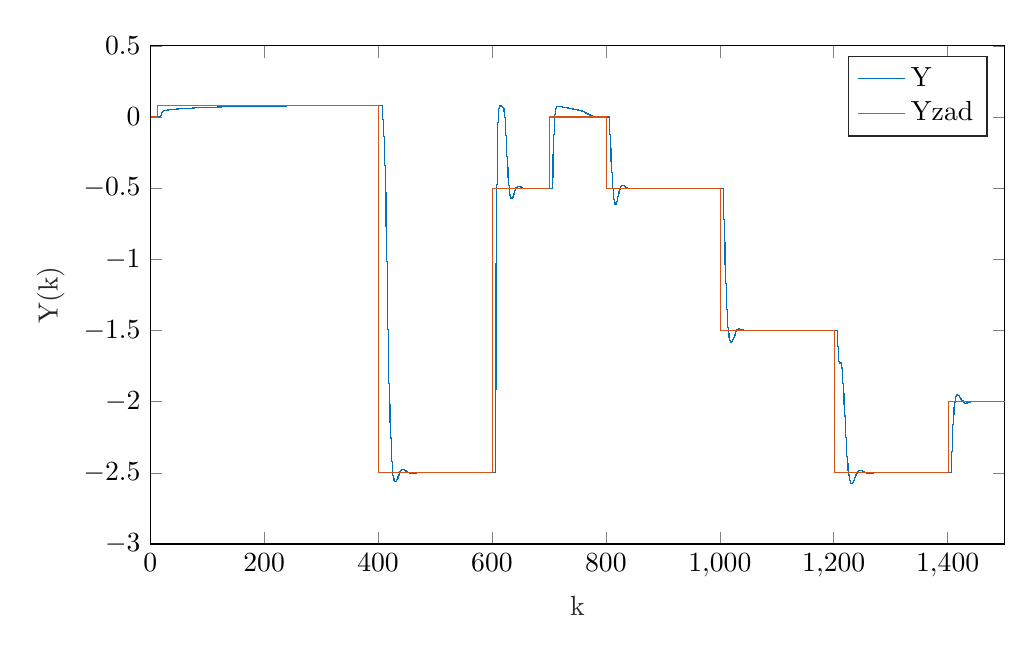
\begin{tikzpicture}

\begin{axis}[%
width=4.272in,
height=2.491in,
at={(0.717in,0.423in)},
scale only axis,
xmin=0,
xmax=1500,
xlabel style={font=\color{white!15!black}},
xlabel={k},
ymin=-3,
ymax=0.5,
ylabel style={font=\color{white!15!black}},
ylabel={Y(k)},
axis background/.style={fill=white},
legend style={legend cell align=left, align=left, draw=white!15!black}
]
\addplot[const plot, color=mycolor1] table[row sep=crcr] {%
1	0\\
2	0\\
3	0\\
4	0\\
5	0\\
6	0\\
7	0\\
8	0\\
9	0\\
10	0\\
11	0\\
12	0\\
13	0\\
14	0\\
15	0\\
16	0\\
17	0.00377487582098053\\
18	0.0121165796854498\\
19	0.0214892581742856\\
20	0.0293495237492624\\
21	0.0349796571224102\\
22	0.0386943390413614\\
23	0.0411288632589746\\
24	0.0428414177952698\\
25	0.0441882270028053\\
26	0.0453426374865372\\
27	0.0463649305228489\\
28	0.0472698618604964\\
29	0.0480667378052365\\
30	0.0487718841587221\\
31	0.0494056996050982\\
32	0.0499861462972479\\
33	0.0505252645285037\\
34	0.0510314026265344\\
35	0.0515108444121446\\
36	0.0519680256721666\\
37	0.0524060964461394\\
38	0.0528273710561351\\
39	0.0532336262852385\\
40	0.0536262835652762\\
41	0.0540065167722303\\
42	0.0543753193465784\\
43	0.0547335485315539\\
44	0.0550819555343038\\
45	0.0554212064632858\\
46	0.0557518971281454\\
47	0.0560745637979555\\
48	0.0563896913239477\\
49	0.0566977195311854\\
50	0.0569990484387615\\
51	0.0572940426482099\\
52	0.057583035108162\\
53	0.0578663303875269\\
54	0.0581442075464174\\
55	0.058416922669102\\
56	0.0586847111081118\\
57	0.0589477894787765\\
58	0.0592063574365718\\
59	0.0594605992645066\\
60	0.0597106852937391\\
61	0.0599567731773256\\
62	0.0601990090342842\\
63	0.0604375284788614\\
64	0.0606724575479518\\
65	0.0609039135379599\\
66	0.06113200576098\\
67	0.0613568362289509\\
68	0.0615785002733942\\
69	0.0617970871074396\\
70	0.0620126803360581\\
71	0.0622253572439468\\
72	0.0624351808645344\\
73	0.0626422039456092\\
74	0.0628464814039486\\
75	0.0630480701831484\\
76	0.0632470272666609\\
77	0.0634434082620313\\
78	0.0636372667425744\\
79	0.0638286540554788\\
80	0.0640176193181794\\
81	0.064204209485408\\
82	0.0643884694466152\\
83	0.0645704421384046\\
84	0.0647501686634397\\
85	0.0649276884098516\\
86	0.0651030391670985\\
87	0.0652762572358899\\
88	0.0654473775310303\\
89	0.0656164336768578\\
90	0.0657834580954106\\
91	0.0659484820876949\\
92	0.0661115359085159\\
93	0.066272648835364\\
94	0.0664318492318299\\
95	0.0665891646059968\\
96	0.0667446216642254\\
97	0.0668982463607132\\
98	0.0670500639431762\\
99	0.0672000989949738\\
100	0.0673483754739693\\
101	0.067494916748393\\
102	0.0676397456299527\\
103	0.0677828844044161\\
104	0.0679243548598699\\
105	0.0680641783128433\\
106	0.0682023756324696\\
107	0.0683389672628416\\
108	0.0684739732437076\\
109	0.06860741322964\\
110	0.0687393065077991\\
111	0.0688696720144027\\
112	0.068998528350006\\
113	0.0691258937936858\\
114	0.0692517863162146\\
115	0.0693762235923056\\
116	0.0694992230120016\\
117	0.0696208016912752\\
118	0.0697409764819014\\
119	0.0698597639806612\\
120	0.0699771805379268\\
121	0.070093242265678\\
122	0.0702079650449938\\
123	0.0703213645330591\\
124	0.0704334561697256\\
125	0.0705442551836603\\
126	0.070653776598114\\
127	0.0707620352363389\\
128	0.070869045726682\\
129	0.0709748225073805\\
130	0.0710793798310797\\
131	0.0711827317690968\\
132	0.0712848922154488\\
133	0.0713858748906627\\
134	0.0714856933453839\\
135	0.0715843609637996\\
136	0.0716818909668887\\
137	0.0717782964155136\\
138	0.0718735902133636\\
139	0.071967785109763\\
140	0.0720608937023515\\
141	0.0721529284396484\\
142	0.072243901623508\\
143	0.0723338254114741\\
144	0.0724227118190414\\
145	0.0725105727218297\\
146	0.072597420055838\\
147	0.0726832669000181\\
148	0.0727681277318413\\
149	0.0728520157623183\\
150	0.0729349430586496\\
151	0.0730169209712509\\
152	0.0730979604258631\\
153	0.0731780720754905\\
154	0.0732572663709664\\
155	0.0733355535987086\\
156	0.0734129439038986\\
157	0.0734894473053824\\
158	0.0735650737051988\\
159	0.0736398328946101\\
160	0.0737137345579638\\
161	0.0737867882752747\\
162	0.0738590035240806\\
163	0.0739303896808973\\
164	0.0740009560224527\\
165	0.0740707117267994\\
166	0.0741396658743578\\
167	0.0742078274489172\\
168	0.0742752053386089\\
169	0.0743418083368602\\
170	0.0744076451433316\\
171	0.0744727243648409\\
172	0.0745370545162758\\
173	0.074600644021494\\
174	0.0746635012142141\\
175	0.0747256343388961\\
176	0.0747870515516123\\
177	0.0748477609209095\\
178	0.0749077704286622\\
179	0.0749670879709174\\
180	0.0750257213587316\\
181	0.0750836783189999\\
182	0.0751409664952771\\
183	0.0751975934485917\\
184	0.0752535666582531\\
185	0.0753088935226509\\
186	0.0753635813600481\\
187	0.0754176374093672\\
188	0.0754710688309698\\
189	0.0755238827074297\\
190	0.0755760860443001\\
191	0.0756276857708736\\
192	0.0756786887409365\\
193	0.0757291017335177\\
194	0.0757789314536302\\
195	0.0758281845330079\\
196	0.0758768675308356\\
197	0.0759249869344736\\
198	0.0759725491601767\\
199	0.0760195605538066\\
200	0.0760660273915398\\
201	0.0761119558805686\\
202	0.0761573521597975\\
203	0.0762022223005332\\
204	0.0762465723071695\\
205	0.0762904081178664\\
206	0.076333735605224\\
207	0.0763765605769504\\
208	0.0764188887765246\\
209	0.0764607258838536\\
210	0.0765020775159244\\
211	0.0765429492274501\\
212	0.0765833465115113\\
213	0.0766232748001913\\
214	0.076662739465207\\
215	0.076701745818533\\
216	0.0767402991130222\\
217	0.0767784045430195\\
218	0.0768160672449709\\
219	0.0768532922980276\\
220	0.0768900847246447\\
221	0.076926449491174\\
222	0.0769623915084528\\
223	0.0769979156323863\\
224	0.0770330266645262\\
225	0.0770677293526428\\
226	0.0771020283912926\\
227	0.0771359284223815\\
228	0.0771694340357214\\
229	0.0772025497695831\\
230	0.0772352801112437\\
231	0.0772676294975288\\
232	0.0772996023153498\\
233	0.077331202902237\\
234	0.0773624355468663\\
235	0.0773933044895826\\
236	0.077423813922917\\
237	0.0774539679921\\
238	0.0774837707955697\\
239	0.0775132263854748\\
240	0.0775423387681736\\
241	0.0775711119047273\\
242	0.0775995497113895\\
243	0.0776276560600903\\
244	0.0776554347789164\\
245	0.0776828896525859\\
246	0.0777100244229192\\
247	0.0777368427893044\\
248	0.0777633484091594\\
249	0.0777895448983883\\
250	0.0778154358318342\\
251	0.0778410247437269\\
252	0.0778663151281268\\
253	0.0778913104393637\\
254	0.0779160140924719\\
255	0.0779404294636209\\
256	0.0779645598905411\\
257	0.077988408672946\\
258	0.0780119790729502\\
259	0.0780352743154824\\
260	0.0780582975886953\\
261	0.0780810520443702\\
262	0.0781035407983187\\
263	0.0781257669307795\\
264	0.0781477334868112\\
265	0.0781694434766817\\
266	0.0781908998762528\\
267	0.0782121056273616\\
268	0.0782330636381973\\
269	0.0782537767836749\\
270	0.0782742479058042\\
271	0.0782944798140559\\
272	0.0783144752857227\\
273	0.078334237066278\\
274	0.07835376786973\\
275	0.0783730703789724\\
276	0.0783921472461312\\
277	0.0784110010929083\\
278	0.0784296345109212\\
279	0.0784480500620392\\
280	0.0784662502787159\\
281	0.0784842376643186\\
282	0.0785020146934538\\
283	0.0785195838122898\\
284	0.0785369474388751\\
285	0.0785541079634541\\
286	0.0785710677487791\\
287	0.0785878291304194\\
288	0.0786043944170665\\
289	0.0786207658908364\\
290	0.0786369458075687\\
291	0.0786529363971225\\
292	0.0786687398636689\\
293	0.0786843583859809\\
294	0.0786997941177191\\
295	0.078715049187716\\
296	0.0787301257002554\\
297	0.0787450257353502\\
298	0.0787597513490168\\
299	0.0787743045735458\\
300	0.078788687417771\\
301	0.0788029018673347\\
302	0.0788169498849503\\
303	0.0788308334106618\\
304	0.0788445543621011\\
305	0.0788581146347422\\
306	0.078871516102152\\
307	0.0788847606162397\\
308	0.0788978500075021\\
309	0.0789107860852671\\
310	0.0789235706379345\\
311	0.0789362054332134\\
312	0.078948692218358\\
313	0.0789610327204003\\
314	0.07897322864638\\
315	0.0789852816835725\\
316	0.078997193499714\\
317	0.0790089657432242\\
318	0.0790206000434263\\
319	0.0790320980107653\\
320	0.0790434612370229\\
321	0.0790546912955308\\
322	0.0790657897413816\\
323	0.0790767581116365\\
324	0.0790875979255321\\
325	0.0790983106846835\\
326	0.0791088978732864\\
327	0.0791193609583158\\
328	0.0791297013897234\\
329	0.0791399206006325\\
330	0.0791500200075305\\
331	0.0791600010104594\\
332	0.0791698649932046\\
333	0.0791796133234808\\
334	0.0791892473531166\\
335	0.0791987684182364\\
336	0.0792081778394407\\
337	0.0792174769219844\\
338	0.0792266669559526\\
339	0.0792357492164353\\
340	0.0792447249636989\\
341	0.0792535954433573\\
342	0.0792623618865397\\
343	0.0792710255100575\\
344	0.0792795875165687\\
345	0.0792880490947407\\
346	0.0792964114194115\\
347	0.0793046756517484\\
348	0.0793128429394059\\
349	0.0793209144166809\\
350	0.0793288912046667\\
351	0.0793367744114051\\
352	0.0793445651320367\\
353	0.0793522644489496\\
354	0.0793598734319267\\
355	0.0793673931382904\\
356	0.0793748246130473\\
357	0.0793821688890292\\
358	0.0793894269870343\\
359	0.079396599915966\\
360	0.0794036886729701\\
361	0.0794106942435703\\
362	0.079417617601803\\
363	0.0794244597103496\\
364	0.0794312215206679\\
365	0.0794379039731216\\
366	0.0794445079971087\\
367	0.0794510345111882\\
368	0.0794574844232057\\
369	0.0794638586304168\\
370	0.07947015801961\\
371	0.079476383467228\\
372	0.0794825358394869\\
373	0.0794886159924948\\
374	0.0794946247723691\\
375	0.0795005630153517\\
376	0.0795064315479239\\
377	0.0795122311869189\\
378	0.0795179627396343\\
379	0.0795236270039417\\
380	0.0795292247683969\\
381	0.0795347568123471\\
382	0.0795402239060381\\
383	0.07954562681072\\
384	0.0795509662787507\\
385	0.0795562430537003\\
386	0.0795614578704518\\
387	0.0795666114553027\\
388	0.0795717045260646\\
389	0.0795767377921613\\
390	0.0795817119547265\\
391	0.0795866277066998\\
392	0.0795914857329223\\
393	0.0795962867102302\\
394	0.079601031307548\\
395	0.0796057201859802\\
396	0.0796103539989027\\
397	0.079614933392052\\
398	0.0796194590036143\\
399	0.0796239314643134\\
400	0.0796283513974971\\
401	0.0796327194192232\\
402	0.0796370361383442\\
403	0.0796413021565912\\
404	0.0796455180686568\\
405	0.0796496844622766\\
406	0.0831438376558065\\
407	0.0561964098429241\\
408	-0.0163950277607965\\
409	-0.0797954890643968\\
410	-0.134480811612989\\
411	-0.209986594485851\\
412	-0.340165358836649\\
413	-0.533745140006509\\
414	-0.768149973517878\\
415	-1.01724559226505\\
416	-1.26319713867793\\
417	-1.49292860702811\\
418	-1.69729863372444\\
419	-1.87288371373\\
420	-2.0216313926538\\
421	-2.14793010249663\\
422	-2.25526536757179\\
423	-2.34519991073497\\
424	-2.41915797935746\\
425	-2.47850747122437\\
426	-2.51910454701821\\
427	-2.54279725306214\\
428	-2.55502044422518\\
429	-2.56049314593788\\
430	-2.56225558732199\\
431	-2.56118595345922\\
432	-2.55695588310564\\
433	-2.54941546050429\\
434	-2.53911238636085\\
435	-2.52719148575206\\
436	-2.51501423955779\\
437	-2.50376934931891\\
438	-2.49424901154753\\
439	-2.48679258645003\\
440	-2.48137411167115\\
441	-2.47776857871594\\
442	-2.47569995612524\\
443	-2.47491965218392\\
444	-2.47522163510294\\
445	-2.4764256556948\\
446	-2.47846786629506\\
447	-2.48116481758485\\
448	-2.48423085246386\\
449	-2.48739089184005\\
450	-2.49043765967357\\
451	-2.49325839242646\\
452	-2.4958109142765\\
453	-2.49807729587964\\
454	-2.50003681237285\\
455	-2.5016619679503\\
456	-2.50292843684974\\
457	-2.50382758917446\\
458	-2.50437330964898\\
459	-2.50460144951285\\
460	-2.50456340979097\\
461	-2.5043170821276\\
462	-2.50391891092825\\
463	-2.50341919305348\\
464	-2.50286056841012\\
465	-2.50227843873221\\
466	-2.50169959169448\\
467	-2.50114755718924\\
468	-2.50064343031331\\
469	-2.5002035492657\\
470	-2.4998378983484\\
471	-2.49954964239788\\
472	-2.49933638763852\\
473	-2.49919238937757\\
474	-2.49911035456441\\
475	-2.4990823923818\\
476	-2.49910027922962\\
477	-2.49915544636552\\
478	-2.49923904851704\\
479	-2.49934223776516\\
480	-2.49945659617811\\
481	-2.49957459610612\\
482	-2.49968994776464\\
483	-2.49979775870549\\
484	-2.49989451400509\\
485	-2.49997793881797\\
486	-2.50004686359761\\
487	-2.50010094741148\\
488	-2.50014048648841\\
489	-2.50016632244758\\
490	-2.50017976209778\\
491	-2.50018247766329\\
492	-2.50017636725679\\
493	-2.50016339642424\\
494	-2.5001454633994\\
495	-2.50012430982249\\
496	-2.50010147527266\\
497	-2.50007828058611\\
498	-2.5000558236108\\
499	-2.50003497838068\\
500	-2.50001639617102\\
501	-2.50000051116807\\
502	-2.49998755418658\\
503	-2.49997757565544\\
504	-2.49997047605494\\
505	-2.49996604004022\\
506	-2.49996396921324\\
507	-2.49996391466087\\
508	-2.49996550404865\\
509	-2.49996836197011\\
510	-2.49997212558521\\
511	-2.499976457043\\
512	-2.4999810537574\\
513	-2.49998565641729\\
514	-2.49999005385609\\
515	-2.49999408436055\\
516	-2.49999763378321\\
517	-2.50000063137778\\
518	-2.50000304438998\\
519	-2.50000487217839\\
520	-2.50000614029166\\
521	-2.50000689467333\\
522	-2.50000719605897\\
523	-2.50000711464778\\
524	-2.50000672519399\\
525	-2.50000610269766\\
526	-2.50000531887114\\
527	-2.50000443937975\\
528	-2.50000352192122\\
529	-2.50000261510943\\
530	-2.50000175802177\\
531	-2.50000098025997\\
532	-2.50000030238887\\
533	-2.49999973665988\\
534	-2.49999928796034\\
535	-2.49999895493219\\
536	-2.49999873119043\\
537	-2.49999860656181\\
538	-2.49999856826988\\
539	-2.49999860201038\\
540	-2.49999869288456\\
541	-2.49999882617758\\
542	-2.49999898798187\\
543	-2.49999916567143\\
544	-2.49999934823517\\
545	-2.49999952647951\\
546	-2.49999969311183\\
547	-2.49999984272248\\
548	-2.4999999716828\\
549	-2.50000007797838\\
550	-2.50000016099843\\
551	-2.50000022130053\\
552	-2.50000026036737\\
553	-2.50000028036823\\
554	-2.50000028393437\\
555	-2.50000027395491\\
556	-2.50000025339815\\
557	-2.50000022516176\\
558	-2.50000019195369\\
559	-2.50000015620411\\
560	-2.50000012000662\\
561	-2.50000008508604\\
562	-2.50000005278902\\
563	-2.50000002409337\\
564	-2.49999999963231\\
565	-2.49999997972955\\
566	-2.499999964442\\
567	-2.4999999536065\\
568	-2.49999994688805\\
569	-2.49999994382692\\
570	-2.49999994388276\\
571	-2.49999994647419\\
572	-2.49999995101278\\
573	-2.49999995693111\\
574	-2.49999996370453\\
575	-2.499999970867\\
576	-2.49999997802131\\
577	-2.49999998484436\\
578	-2.49999999108807\\
579	-2.49999999657674\\
580	-2.50000000120154\\
581	-2.50000000491307\\
582	-2.50000000771255\\
583	-2.50000000964233\\
584	-2.50000001077633\\
585	-2.50000001121087\\
586	-2.5000000110561\\
587	-2.50000001042845\\
588	-2.50000000944419\\
589	-2.50000000821422\\
590	-2.50000000683995\\
591	-2.50000000541053\\
592	-2.50000000400106\\
593	-2.50000000267178\\
594	-2.50000000146811\\
595	-2.50000000042133\\
596	-2.4999999995498\\
597	-2.49999999886052\\
598	-2.49999999835092\\
599	-2.49999999801077\\
600	-2.49999999782403\\
601	-2.49999999777069\\
602	-2.49999999782839\\
603	-2.49999999797391\\
604	-2.49999999818432\\
605	-2.49999999843804\\
606	-1.91692412349649\\
607	-1.03081361501881\\
608	-0.473146089497253\\
609	-0.181926264652505\\
610	-0.0394178477610559\\
611	0.0284713548656605\\
612	0.0604323697441411\\
613	0.0751399378830727\\
614	0.0808368752212398\\
615	0.0812482559254594\\
616	0.0786697994412446\\
617	0.0745905129917868\\
618	0.0698762715601322\\
619	0.0646808405205015\\
620	0.0580930972703068\\
621	0.0399116148264566\\
622	-0.0041330209290792\\
623	-0.0645562408584274\\
624	-0.131199359863292\\
625	-0.201888136899772\\
626	-0.278163100095099\\
627	-0.355135855488057\\
628	-0.424460167234268\\
629	-0.480391658376555\\
630	-0.521286848957126\\
631	-0.548336539919586\\
632	-0.563964588348314\\
633	-0.571182497842235\\
634	-0.572455279544839\\
635	-0.569267838447915\\
636	-0.562467692851404\\
637	-0.552763374135235\\
638	-0.541115425143017\\
639	-0.528788826063066\\
640	-0.517084601700759\\
641	-0.507003147609429\\
642	-0.499055183705412\\
643	-0.493287656645079\\
644	-0.489458656713807\\
645	-0.487236859339321\\
646	-0.486307396659928\\
647	-0.486503930202179\\
648	-0.487654834761472\\
649	-0.489492188406417\\
650	-0.491695646821276\\
651	-0.493971189914617\\
652	-0.496102842579681\\
653	-0.497957617740788\\
654	-0.499476568049814\\
655	-0.500651897717252\\
656	-0.501501337618584\\
657	-0.502052536548659\\
658	-0.502337026800985\\
659	-0.502390979725279\\
660	-0.502257919878823\\
661	-0.501988510448543\\
662	-0.501636124414237\\
663	-0.501250157069391\\
664	-0.500870242792356\\
665	-0.5005236697356\\
666	-0.500226500698774\\
667	-0.499985130025198\\
668	-0.499801275864808\\
669	-0.499674346034021\\
670	-0.499601027353631\\
671	-0.499574794168744\\
672	-0.499586450814015\\
673	-0.499625627529018\\
674	-0.499682219154583\\
675	-0.499747455166443\\
676	-0.499814422227402\\
677	-0.499878059134944\\
678	-0.499934895633287\\
679	-0.499982739112314\\
680	-0.500020423405976\\
681	-0.500047651513556\\
682	-0.500064884895358\\
683	-0.500073213940156\\
684	-0.50007417497738\\
685	-0.50006952569888\\
686	-0.500061021601314\\
687	-0.500050264468352\\
688	-0.500038580181037\\
689	-0.500026995174882\\
690	-0.500016275351064\\
691	-0.500006962188832\\
692	-0.499999390522707\\
693	-0.499993698699229\\
694	-0.499989851920596\\
695	-0.499987680488401\\
696	-0.499986926792784\\
697	-0.499987291772105\\
698	-0.499988471893923\\
699	-0.499990183927678\\
700	-0.499992179082058\\
701	-0.499994249711872\\
702	-0.499996231822446\\
703	-0.499998005307072\\
704	-0.49999949245143\\
705	-0.500000654496857\\
706	-0.426626133264708\\
707	-0.265156238062627\\
708	-0.122313602137289\\
709	-0.0317000607404464\\
710	0.0180440060790192\\
711	0.044558096649409\\
712	0.0591042059859875\\
713	0.067195656728085\\
714	0.0715390618072864\\
715	0.0736411848281907\\
716	0.0744217564648613\\
717	0.0744485236883952\\
718	0.0740613159359453\\
719	0.0734556762086128\\
720	0.0727400723826983\\
721	0.0719726942522437\\
722	0.0711841017679242\\
723	0.0703900327978104\\
724	0.0695983576221966\\
725	0.0688128361238931\\
726	0.0680351164269738\\
727	0.0672657733832668\\
728	0.0665048307604148\\
729	0.065752014001552\\
730	0.0650068671480346\\
731	0.0642688038614402\\
732	0.0635371275854101\\
733	0.062811045614073\\
734	0.0620897746878287\\
735	0.0613725049368553\\
736	0.0606582537413348\\
737	0.0599458654311089\\
738	0.0592340335331095\\
739	0.0585213179715441\\
740	0.0578061546276342\\
741	0.0570868602538683\\
742	0.0563616361480243\\
743	0.0556285723084807\\
744	0.054885652878891\\
745	0.0541307633601608\\
746	0.0533616999745979\\
747	0.0525761815434287\\
748	0.0517718379420178\\
749	0.0509450195869525\\
750	0.0500850525985303\\
751	0.0491812492280774\\
752	0.0482240942525082\\
753	0.0472050543118716\\
754	0.0461163055975985\\
755	0.044950530326957\\
756	0.0437007728265487\\
757	0.0423602816203539\\
758	0.0409224615710112\\
759	0.0393811087820766\\
760	0.0377309789677922\\
761	0.0359685869039328\\
762	0.0340930537479006\\
763	0.0321068493870715\\
764	0.0300163800185842\\
765	0.027835714415585\\
766	0.0255891021255402\\
767	0.0233052180143587\\
768	0.0210141537496898\\
769	0.0187465734750693\\
770	0.0165332331798326\\
771	0.0144039455359359\\
772	0.0123860622753174\\
773	0.0105030884532735\\
774	0.00877376428840681\\
775	0.00721160286334752\\
776	0.00582472508783233\\
777	0.00461586819669011\\
778	0.0035825540386172\\
779	0.00271747518350067\\
780	0.00200914778839061\\
781	0.00144281611836092\\
782	0.00100152476133771\\
783	0.000667236973873652\\
784	0.000421879516249313\\
785	0.000248223740536668\\
786	0.000130551887550087\\
787	5.50935158901762e-05\\
788	1.02441417790179e-05\\
789	-1.34038884320716e-05\\
790	-2.31780245856838e-05\\
791	-2.45453237093326e-05\\
792	-2.1392197061781e-05\\
793	-1.63260250245521e-05\\
794	-1.09685810228481e-05\\
795	-6.22046202177101e-06\\
796	-2.48469728605997e-06\\
797	1.54732409970749e-07\\
798	1.79815770127754e-06\\
799	2.63442344973679e-06\\
800	2.87740553925464e-06\\
801	2.72774344892511e-06\\
802	2.35308494936476e-06\\
803	1.88102811967862e-06\\
804	1.40005106451565e-06\\
805	9.64850662496701e-07\\
806	-0.0363155918295903\\
807	-0.12018333628385\\
808	-0.218675529250397\\
809	-0.31078435335384\\
810	-0.387115308446487\\
811	-0.449493975703346\\
812	-0.501935873505197\\
813	-0.545682703937599\\
814	-0.579685436879158\\
815	-0.602437908065749\\
816	-0.613534462677262\\
817	-0.614102562237651\\
818	-0.606327366787558\\
819	-0.592750508504184\\
820	-0.575775634256405\\
821	-0.557451785434581\\
822	-0.539421146365724\\
823	-0.522920659406349\\
824	-0.508793461586289\\
825	-0.497510401451132\\
826	-0.488553111617633\\
827	-0.482300602265211\\
828	-0.479010615731818\\
829	-0.478326505535505\\
830	-0.479579971596414\\
831	-0.482006655269804\\
832	-0.485007787421439\\
833	-0.488217238045258\\
834	-0.491416121537025\\
835	-0.494444704296551\\
836	-0.497160698913329\\
837	-0.499444576293285\\
838	-0.501221986280014\\
839	-0.502475548515956\\
840	-0.503238694783823\\
841	-0.503578525547223\\
842	-0.503577776560209\\
843	-0.503321814609682\\
844	-0.502891332603499\\
845	-0.502358736741646\\
846	-0.501793917031079\\
847	-0.501237639315214\\
848	-0.500720837596066\\
849	-0.500272142165641\\
850	-0.499911444200588\\
851	-0.499647476317094\\
852	-0.499476738179601\\
853	-0.499386970453554\\
854	-0.499362567041856\\
855	-0.499388167340055\\
856	-0.499449971820863\\
857	-0.499535645027366\\
858	-0.499634010080775\\
859	-0.499735190651469\\
860	-0.499831098288713\\
861	-0.499915866665141\\
862	-0.499985951589045\\
863	-0.500039875548935\\
864	-0.500077770575392\\
865	-0.500100893621899\\
866	-0.500111124721307\\
867	-0.500110989491282\\
868	-0.500103071845781\\
869	-0.500089745599449\\
870	-0.500073186123269\\
871	-0.50005531934094\\
872	-0.500037771316866\\
873	-0.50002178550876\\
874	-0.500008168282581\\
875	-0.499997317845928\\
876	-0.49998931072121\\
877	-0.499984001986053\\
878	-0.499981106328506\\
879	-0.499980251628141\\
880	-0.499981015829927\\
881	-0.499982959471586\\
882	-0.499985658177315\\
883	-0.499988731861227\\
884	-0.499991865332582\\
885	-0.499994817702942\\
886	-0.499997422888667\\
887	-0.499999577999909\\
888	-0.500001238641759\\
889	-0.500002408049181\\
890	-0.500003122856965\\
891	-0.500003442003676\\
892	-0.500003437429523\\
893	-0.50000318690102\\
894	-0.500002767915085\\
895	-0.500002252048007\\
896	-0.500001700562002\\
897	-0.500001161948984\\
898	-0.500000671466817\\
899	-0.500000252124118\\
900	-0.499999916352634\\
901	-0.499999667836184\\
902	-0.499999503305896\\
903	-0.499999414307537\\
904	-0.499999388953908\\
905	-0.49999941359156\\
906	-0.499999474242162\\
907	-0.499999557793481\\
908	-0.499999652683905\\
909	-0.499999749349564\\
910	-0.499999840449781\\
911	-0.499999920840312\\
912	-0.499999987392712\\
913	-0.500000038711887\\
914	-0.50000007481095\\
915	-0.500000096782336\\
916	-0.500000106473133\\
917	-0.50000010617499\\
918	-0.50000009834632\\
919	-0.500000085386021\\
920	-0.500000069470481\\
921	-0.50000005245274\\
922	-0.500000035813032\\
923	-0.500000020647421\\
924	-0.500000007683702\\
925	-0.499999997317271\\
926	-0.499999989661586\\
927	-0.499999984606611\\
928	-0.499999981882164\\
929	-0.499999981116745\\
930	-0.499999981888726\\
931	-0.499999983769051\\
932	-0.499999986353876\\
933	-0.499999989287357\\
934	-0.499999992275282\\
935	-0.499999995090844\\
936	-0.499999997574337\\
937	-0.499999999628386\\
938	-0.500000001210005\\
939	-0.500000002320637\\
940	-0.500000002995268\\
941	-0.500000003291663\\
942	-0.500000003280572\\
943	-0.500000003037468\\
944	-0.500000002636033\\
945	-0.500000002143384\\
946	-0.500000001616907\\
947	-0.500000001102525\\
948	-0.50000000063415\\
949	-0.500000000234151\\
950	-0.49999999991456\\
951	-0.49999999967872\\
952	-0.49999999952316\\
953	-0.499999999439508\\
954	-0.499999999416282\\
955	-0.499999999440471\\
956	-0.499999999498832\\
957	-0.499999999578896\\
958	-0.499999999669663\\
959	-0.499999999762034\\
960	-0.499999999849004\\
961	-0.499999999925656\\
962	-0.499999999989009\\
963	-0.500000000037762\\
964	-0.500000000071971\\
965	-0.500000000092722\\
966	-0.500000000101798\\
967	-0.500000000101383\\
968	-0.500000000093811\\
969	-0.500000000081363\\
970	-0.500000000066114\\
971	-0.500000000049836\\
972	-0.500000000033944\\
973	-0.500000000019483\\
974	-0.50000000000714\\
975	-0.499999999997284\\
976	-0.499999999990015\\
977	-0.499999999985227\\
978	-0.499999999982659\\
979	-0.499999999981956\\
980	-0.499999999982715\\
981	-0.499999999984527\\
982	-0.499999999987007\\
983	-0.499999999989814\\
984	-0.499999999992669\\
985	-0.499999999995355\\
986	-0.499999999997721\\
987	-0.499999999999675\\
988	-0.500000000001178\\
989	-0.500000000002232\\
990	-0.50000000000287\\
991	-0.500000000003148\\
992	-0.500000000003132\\
993	-0.500000000002897\\
994	-0.500000000002511\\
995	-0.500000000002039\\
996	-0.500000000001536\\
997	-0.500000000001045\\
998	-0.500000000000599\\
999	-0.500000000000218\\
1000	-0.499999999999914\\
1001	-0.49999999999969\\
1002	-0.499999999999543\\
1003	-0.499999999999464\\
1004	-0.499999999999442\\
1005	-0.499999999999466\\
1006	-0.573098658676213\\
1007	-0.717303851822164\\
1008	-0.882713589434291\\
1009	-1.03764381475606\\
1010	-1.16724483776827\\
1011	-1.27126602183646\\
1012	-1.35500183712723\\
1013	-1.42292208141866\\
1014	-1.47743758905225\\
1015	-1.51963363643396\\
1016	-1.5502916696806\\
1017	-1.57048214667604\\
1018	-1.58167775381477\\
1019	-1.58560300761793\\
1020	-1.58402069724138\\
1021	-1.57856346600538\\
1022	-1.57063807698192\\
1023	-1.56138959983271\\
1024	-1.55170371784687\\
1025	-1.54222956567157\\
1026	-1.53133035294984\\
1027	-1.51967589428975\\
1028	-1.5090106974149\\
1029	-1.50053837903566\\
1030	-1.49468895805524\\
1031	-1.49119994660362\\
1032	-1.48948721494082\\
1033	-1.48897307178718\\
1034	-1.48922556952058\\
1035	-1.48996576299218\\
1036	-1.49101804299194\\
1037	-1.49225931161066\\
1038	-1.49358955254483\\
1039	-1.49492243347766\\
1040	-1.49618647986404\\
1041	-1.49732847503836\\
1042	-1.4983148489115\\
1043	-1.49913025175125\\
1044	-1.49977419867229\\
1045	-1.50025700282467\\
1046	-1.50063928218724\\
1047	-1.50093869362205\\
1048	-1.50113706463546\\
1049	-1.50121973007703\\
1050	-1.50119114421747\\
1051	-1.50107665076456\\
1052	-1.5009116553851\\
1053	-1.50072896414778\\
1054	-1.50055184227154\\
1055	-1.50039308389435\\
1056	-1.50025762799322\\
1057	-1.50014597256956\\
1058	-1.50005674490378\\
1059	-1.49998803970119\\
1060	-1.49993784426094\\
1061	-1.49990403803975\\
1062	-1.49988432175648\\
1063	-1.49987622995284\\
1064	-1.49987723679243\\
1065	-1.49988490386978\\
1066	-1.49989609509359\\
1067	-1.49990888866966\\
1068	-1.4999227406168\\
1069	-1.4999375249707\\
1070	-1.49995287774072\\
1071	-1.49996797154468\\
1072	-1.49998175093593\\
1073	-1.49999332564104\\
1074	-1.50000222532831\\
1075	-1.5000084346247\\
1076	-1.50001226880189\\
1077	-1.50001419873191\\
1078	-1.50001470839856\\
1079	-1.50001421653591\\
1080	-1.5000130543519\\
1081	-1.50001147511026\\
1082	-1.5000096732712\\
1083	-1.5000078004676\\
1084	-1.50000597470202\\
1085	-1.50000428437365\\
1086	-1.50000280976248\\
1087	-1.50000158853365\\
1088	-1.5000006098156\\
1089	-1.49999983988006\\
1090	-1.499999246828\\
1091	-1.49999881322115\\
1092	-1.49999853291772\\
1093	-1.49999839982653\\
1094	-1.49999839888648\\
1095	-1.49999850402152\\
1096	-1.49999868223244\\
1097	-1.49999890013589\\
1098	-1.49999912944045\\
1099	-1.49999934966143\\
1100	-1.49999954817239\\
1101	-1.4999997186509\\
1102	-1.49999985906787\\
1103	-1.4999999699727\\
1104	-1.500000053344\\
1105	-1.50000011194469\\
1106	-1.50000014857408\\
1107	-1.50000016660604\\
1108	-1.50000017015606\\
1109	-1.50000016346225\\
1110	-1.50000015015309\\
1111	-1.50000013282747\\
1112	-1.50000011313736\\
1113	-1.50000009219488\\
1114	-1.5000000709721\\
1115	-1.50000005048532\\
1116	-1.5000000317478\\
1117	-1.50000001560395\\
1118	-1.50000000257904\\
1119	-1.49999999282315\\
1120	-1.49999998615635\\
1121	-1.49999998217571\\
1122	-1.49999998037402\\
1123	-1.4999999802346\\
1124	-1.49999998128877\\
1125	-1.4999999831398\\
1126	-1.49999998547415\\
1127	-1.49999998803931\\
1128	-1.49999999062454\\
1129	-1.49999999306217\\
1130	-1.4999999952371\\
1131	-1.49999999709102\\
1132	-1.49999999861364\\
1133	-1.49999999982386\\
1134	-1.50000000075084\\
1135	-1.5000000014225\\
1136	-1.50000000186316\\
1137	-1.50000000209706\\
1138	-1.50000000215262\\
1139	-1.50000000206414\\
1140	-1.50000000187013\\
1141	-1.50000000160943\\
1142	-1.50000000131711\\
1143	-1.5000000010215\\
1144	-1.5000000007431\\
1145	-1.50000000049493\\
1146	-1.50000000028366\\
1147	-1.50000000011155\\
1148	-1.49999999997812\\
1149	-1.4999999998811\\
1150	-1.49999999981683\\
1151	-1.49999999978048\\
1152	-1.4999999997665\\
1153	-1.4999999997693\\
1154	-1.49999999978386\\
1155	-1.49999999980613\\
1156	-1.499999999833\\
1157	-1.49999999986217\\
1158	-1.49999999989181\\
1159	-1.4999999999204\\
1160	-1.49999999994667\\
1161	-1.49999999996965\\
1162	-1.49999999998871\\
1163	-1.50000000000358\\
1164	-1.50000000001436\\
1165	-1.50000000002144\\
1166	-1.50000000002535\\
1167	-1.50000000002672\\
1168	-1.50000000002615\\
1169	-1.5000000000242\\
1170	-1.50000000002134\\
1171	-1.50000000001798\\
1172	-1.50000000001445\\
1173	-1.50000000001101\\
1174	-1.50000000000786\\
1175	-1.5000000000051\\
1176	-1.50000000000277\\
1177	-1.5000000000009\\
1178	-1.49999999999945\\
1179	-1.49999999999838\\
1180	-1.49999999999767\\
1181	-1.49999999999725\\
1182	-1.4999999999971\\
1183	-1.49999999999715\\
1184	-1.49999999999735\\
1185	-1.49999999999767\\
1186	-1.49999999999804\\
1187	-1.49999999999843\\
1188	-1.49999999999882\\
1189	-1.49999999999917\\
1190	-1.49999999999948\\
1191	-1.49999999999974\\
1192	-1.49999999999995\\
1193	-1.5000000000001\\
1194	-1.50000000000021\\
1195	-1.50000000000028\\
1196	-1.50000000000031\\
1197	-1.50000000000032\\
1198	-1.50000000000031\\
1199	-1.50000000000028\\
1200	-1.50000000000024\\
1201	-1.5000000000002\\
1202	-1.50000000000016\\
1203	-1.50000000000012\\
1204	-1.50000000000009\\
1205	-1.50000000000005\\
1206	-1.54222913660834\\
1207	-1.61326328503289\\
1208	-1.67840877504907\\
1209	-1.71939630711625\\
1210	-1.73243573079221\\
1211	-1.72916997481365\\
1212	-1.72620307167179\\
1213	-1.73572324781671\\
1214	-1.76333469665091\\
1215	-1.80930898660811\\
1216	-1.87059017400418\\
1217	-1.94261899785901\\
1218	-2.02066411952328\\
1219	-2.1005737127342\\
1220	-2.17904107621842\\
1221	-2.25357665530003\\
1222	-2.32210892100679\\
1223	-2.38325867642908\\
1224	-2.43630853776187\\
1225	-2.48093594282264\\
1226	-2.51510887917041\\
1227	-2.53934852246022\\
1228	-2.55571235001903\\
1229	-2.56610236331821\\
1230	-2.57189229645183\\
1231	-2.57381755892373\\
1232	-2.57225576997925\\
1233	-2.5675884644744\\
1234	-2.56037256296678\\
1235	-2.55133237292202\\
1236	-2.54126075177234\\
1237	-2.530907740141\\
1238	-2.52090129475942\\
1239	-2.51171214115309\\
1240	-2.50365438079602\\
1241	-2.49690633655689\\
1242	-2.49153799653247\\
1243	-2.4875368961373\\
1244	-2.48482946361204\\
1245	-2.48329800775829\\
1246	-2.48283767033498\\
1247	-2.48328031626666\\
1248	-2.48441177804805\\
1249	-2.48602151325639\\
1250	-2.48792777431344\\
1251	-2.48998835944004\\
1252	-2.49209488605861\\
1253	-2.49416055821778\\
1254	-2.49611200005891\\
1255	-2.49788730405022\\
1256	-2.49943802452645\\
1257	-2.50073188318629\\
1258	-2.50175394688926\\
1259	-2.50250560310243\\
1260	-2.50300180034276\\
1261	-2.50326746662652\\
1262	-2.50333392741772\\
1263	-2.50323581376716\\
1264	-2.50300862408969\\
1265	-2.50268689668139\\
1266	-2.50230195638986\\
1267	-2.50188274245443\\
1268	-2.50145533429719\\
1269	-2.50104162603433\\
1270	-2.50065853564516\\
1271	-2.50031783461145\\
1272	-2.5000266674031\\
1273	-2.49978844187489\\
1274	-2.49960368350945\\
1275	-2.49947067967665\\
1276	-2.49938593315931\\
1277	-2.49934452701945\\
1278	-2.49934049001456\\
1279	-2.49936719418615\\
1280	-2.49941776509969\\
1281	-2.4994854628668\\
1282	-2.49956399652058\\
1283	-2.49964775239351\\
1284	-2.49973193590032\\
1285	-2.49981263838162\\
1286	-2.49988686470627\\
1287	-2.49995246228507\\
1288	-2.50000804480076\\
1289	-2.50005292554377\\
1290	-2.50008703629875\\
1291	-2.50011082774444\\
1292	-2.50012515174053\\
1293	-2.50013113751949\\
1294	-2.50013007783116\\
1295	-2.50012333446499\\
1296	-2.50011226470028\\
1297	-2.5000981653772\\
1298	-2.50008223030263\\
1299	-2.50006551819616\\
1300	-2.50004893024724\\
1301	-2.50003319733401\\
1302	-2.50001887684951\\
1303	-2.50000635834739\\
1304	-2.49999587643787\\
1305	-2.4999875289084\\
1306	-2.49998129758409\\
1307	-2.49997707165909\\
1308	-2.49997467057413\\
1309	-2.49997386497523\\
1310	-2.49997439567192\\
1311	-2.49997599050954\\
1312	-2.49997837907678\\
1313	-2.49998130494758\\
1314	-2.49998453508653\\
1315	-2.4999878662865\\
1316	-2.49999112882958\\
1317	-2.49999418779783\\
1318	-2.49999694254006\\
1319	-2.499999324756\\
1320	-2.5000012955678\\
1321	-2.50000284187106\\
1322	-2.50000397221677\\
1323	-2.50000471245955\\
1324	-2.50000510139726\\
1325	-2.50000518660523\\
1326	-2.50000502063986\\
1327	-2.50000465769849\\
1328	-2.5000041508322\\
1329	-2.50000354975234\\
1330	-2.50000289920983\\
1331	-2.50000223790096\\
1332	-2.50000159784027\\
1333	-2.50000100414132\\
1334	-2.50000047514714\\
1335	-2.50000002284766\\
1336	-2.49999965351534\\
1337	-2.49999936848788\\
1338	-2.49999916503077\\
1339	-2.49999903722199\\
1340	-2.49999897681339\\
1341	-2.49999897403472\\
1342	-2.49999901831654\\
1343	-2.49999909891569\\
1344	-2.49999920543401\\
1345	-2.49999932822612\\
1346	-2.49999945869802\\
1347	-2.49999958950281\\
1348	-2.49999971464338\\
1349	-2.49999982949395\\
1350	-2.49999993075487\\
1351	-2.50000001635554\\
1352	-2.5000000853199\\
1353	-2.50000013760763\\
1354	-2.50000017394256\\
1355	-2.50000019563824\\
1356	-2.50000020442886\\
1357	-2.50000020231228\\
1358	-2.50000019141021\\
1359	-2.50000017384879\\
1360	-2.50000015166126\\
1361	-2.50000012671306\\
1362	-2.50000010064846\\
1363	-2.50000007485712\\
1364	-2.50000005045838\\
1365	-2.50000002830061\\
1366	-2.50000000897306\\
1367	-2.49999999282717\\
1368	-2.49999998000471\\
1369	-2.49999997047035\\
1370	-2.4999999640461\\
1371	-2.49999996044592\\
1372	-2.49999995930877\\
1373	-2.49999996022891\\
1374	-2.49999996278261\\
1375	-2.49999996655069\\
1376	-2.49999997113669\\
1377	-2.49999997618067\\
1378	-2.49999998136873\\
1379	-2.49999998643873\\
1380	-2.49999999118257\\
1381	-2.4999999954456\\
1382	-2.4999999991237\\
1383	-2.5000000021586\\
1384	-2.50000000453205\\
1385	-2.50000000625918\\
1386	-2.50000000738165\\
1387	-2.50000000796079\\
1388	-2.50000000807122\\
1389	-2.50000000779496\\
1390	-2.50000000721634\\
1391	-2.50000000641776\\
1392	-2.50000000547629\\
1393	-2.50000000446118\\
1394	-2.50000000343215\\
1395	-2.50000000243848\\
1396	-2.50000000151869\\
1397	-2.50000000070078\\
1398	-2.50000000000295\\
1399	-2.49999999943456\\
1400	-2.49999999899736\\
1401	-2.49999999868683\\
1402	-2.49999999849354\\
1403	-2.49999999840449\\
1404	-2.49999999840436\\
1405	-2.49999999847664\\
1406	-2.44278286051698\\
1407	-2.34863392123394\\
1408	-2.24961342651199\\
1409	-2.16214812361625\\
1410	-2.09215446567747\\
1411	-2.04002119471735\\
1412	-2.0034490565615\\
1413	-1.97921191998834\\
1414	-1.96421721814956\\
1415	-1.95595061430228\\
1416	-1.95252626504335\\
1417	-1.95256335531753\\
1418	-1.9550325510752\\
1419	-1.95913788031491\\
1420	-1.96424575948451\\
1421	-1.9698487815281\\
1422	-1.97554788961489\\
1423	-1.98104114044989\\
1424	-1.98611314069201\\
1425	-1.99062340417959\\
1426	-1.99551025513364\\
1427	-2.00059352567387\\
1428	-2.00511091217808\\
1429	-2.00851696348458\\
1430	-2.01061855262296\\
1431	-2.01151308974655\\
1432	-2.01145623519299\\
1433	-2.01074009437992\\
1434	-2.00962040303827\\
1435	-2.00829036769032\\
1436	-2.0068837351709\\
1437	-2.00548951734156\\
1438	-2.00416700400451\\
1439	-2.00295634356405\\
1440	-2.00188439047623\\
1441	-2.00096740779831\\
1442	-2.0002123749417\\
1443	-1.99961805797553\\
1444	-1.99917632594854\\
1445	-1.99887374147401\\
1446	-1.99867153736264\\
1447	-1.99855178688776\\
1448	-1.99851468184596\\
1449	-1.99855933839124\\
1450	-1.99867613277457\\
1451	-1.99884664768888\\
1452	-1.99904826594039\\
1453	-1.99925950648395\\
1454	-1.99946346418814\\
1455	-1.99964888308307\\
1456	-1.99980954796702\\
1457	-1.99994295904424\\
1458	-2.00004901449244\\
1459	-2.00012903692764\\
1460	-2.00018517877145\\
1461	-2.00022009624343\\
1462	-2.00023676040558\\
1463	-2.00023831409329\\
1464	-2.00022793477227\\
1465	-2.0002086994108\\
1466	-2.00018392448136\\
1467	-2.00015617162136\\
1468	-2.00012711221361\\
1469	-2.00009797156692\\
1470	-2.00006984514151\\
1471	-2.00004380046007\\
1472	-2.00002079239087\\
1473	-2.00000151662008\\
1474	-1.99998631637357\\
1475	-1.99997518122563\\
1476	-1.99996781878248\\
1477	-1.9999637569672\\
1478	-1.99996243996147\\
1479	-1.99996329870164\\
1480	-1.99996579339543\\
1481	-1.9999694347727\\
1482	-1.99997379286659\\
1483	-1.99997850002742\\
1484	-1.99998325166587\\
1485	-1.99998780574783\\
1486	-1.99999197106564\\
1487	-1.99999562161848\\
1488	-1.999998695942\\
1489	-2.00000117963792\\
1490	-2.00000308748439\\
1491	-2.00000445142669\\
1492	-2.00000531579575\\
1493	-2.00000573656387\\
1494	-2.00000578047282\\
1495	-2.00000552195877\\
1496	-2.00000503809477\\
1497	-2.00000440300732\\
1498	-2.00000368324839\\
1499	-2.00000293492404\\
1500	-2.00000220261746\\
};
\addlegendentry{Y}

\addplot[const plot, color=mycolor2] table[row sep=crcr] {%
1	0\\
2	0\\
3	0\\
4	0\\
5	0\\
6	0\\
7	0\\
8	0\\
9	0\\
10	0\\
11	0\\
12	0.08\\
13	0.08\\
14	0.08\\
15	0.08\\
16	0.08\\
17	0.08\\
18	0.08\\
19	0.08\\
20	0.08\\
21	0.08\\
22	0.08\\
23	0.08\\
24	0.08\\
25	0.08\\
26	0.08\\
27	0.08\\
28	0.08\\
29	0.08\\
30	0.08\\
31	0.08\\
32	0.08\\
33	0.08\\
34	0.08\\
35	0.08\\
36	0.08\\
37	0.08\\
38	0.08\\
39	0.08\\
40	0.08\\
41	0.08\\
42	0.08\\
43	0.08\\
44	0.08\\
45	0.08\\
46	0.08\\
47	0.08\\
48	0.08\\
49	0.08\\
50	0.08\\
51	0.08\\
52	0.08\\
53	0.08\\
54	0.08\\
55	0.08\\
56	0.08\\
57	0.08\\
58	0.08\\
59	0.08\\
60	0.08\\
61	0.08\\
62	0.08\\
63	0.08\\
64	0.08\\
65	0.08\\
66	0.08\\
67	0.08\\
68	0.08\\
69	0.08\\
70	0.08\\
71	0.08\\
72	0.08\\
73	0.08\\
74	0.08\\
75	0.08\\
76	0.08\\
77	0.08\\
78	0.08\\
79	0.08\\
80	0.08\\
81	0.08\\
82	0.08\\
83	0.08\\
84	0.08\\
85	0.08\\
86	0.08\\
87	0.08\\
88	0.08\\
89	0.08\\
90	0.08\\
91	0.08\\
92	0.08\\
93	0.08\\
94	0.08\\
95	0.08\\
96	0.08\\
97	0.08\\
98	0.08\\
99	0.08\\
100	0.08\\
101	0.08\\
102	0.08\\
103	0.08\\
104	0.08\\
105	0.08\\
106	0.08\\
107	0.08\\
108	0.08\\
109	0.08\\
110	0.08\\
111	0.08\\
112	0.08\\
113	0.08\\
114	0.08\\
115	0.08\\
116	0.08\\
117	0.08\\
118	0.08\\
119	0.08\\
120	0.08\\
121	0.08\\
122	0.08\\
123	0.08\\
124	0.08\\
125	0.08\\
126	0.08\\
127	0.08\\
128	0.08\\
129	0.08\\
130	0.08\\
131	0.08\\
132	0.08\\
133	0.08\\
134	0.08\\
135	0.08\\
136	0.08\\
137	0.08\\
138	0.08\\
139	0.08\\
140	0.08\\
141	0.08\\
142	0.08\\
143	0.08\\
144	0.08\\
145	0.08\\
146	0.08\\
147	0.08\\
148	0.08\\
149	0.08\\
150	0.08\\
151	0.08\\
152	0.08\\
153	0.08\\
154	0.08\\
155	0.08\\
156	0.08\\
157	0.08\\
158	0.08\\
159	0.08\\
160	0.08\\
161	0.08\\
162	0.08\\
163	0.08\\
164	0.08\\
165	0.08\\
166	0.08\\
167	0.08\\
168	0.08\\
169	0.08\\
170	0.08\\
171	0.08\\
172	0.08\\
173	0.08\\
174	0.08\\
175	0.08\\
176	0.08\\
177	0.08\\
178	0.08\\
179	0.08\\
180	0.08\\
181	0.08\\
182	0.08\\
183	0.08\\
184	0.08\\
185	0.08\\
186	0.08\\
187	0.08\\
188	0.08\\
189	0.08\\
190	0.08\\
191	0.08\\
192	0.08\\
193	0.08\\
194	0.08\\
195	0.08\\
196	0.08\\
197	0.08\\
198	0.08\\
199	0.08\\
200	0.08\\
201	0.08\\
202	0.08\\
203	0.08\\
204	0.08\\
205	0.08\\
206	0.08\\
207	0.08\\
208	0.08\\
209	0.08\\
210	0.08\\
211	0.08\\
212	0.08\\
213	0.08\\
214	0.08\\
215	0.08\\
216	0.08\\
217	0.08\\
218	0.08\\
219	0.08\\
220	0.08\\
221	0.08\\
222	0.08\\
223	0.08\\
224	0.08\\
225	0.08\\
226	0.08\\
227	0.08\\
228	0.08\\
229	0.08\\
230	0.08\\
231	0.08\\
232	0.08\\
233	0.08\\
234	0.08\\
235	0.08\\
236	0.08\\
237	0.08\\
238	0.08\\
239	0.08\\
240	0.08\\
241	0.08\\
242	0.08\\
243	0.08\\
244	0.08\\
245	0.08\\
246	0.08\\
247	0.08\\
248	0.08\\
249	0.08\\
250	0.08\\
251	0.08\\
252	0.08\\
253	0.08\\
254	0.08\\
255	0.08\\
256	0.08\\
257	0.08\\
258	0.08\\
259	0.08\\
260	0.08\\
261	0.08\\
262	0.08\\
263	0.08\\
264	0.08\\
265	0.08\\
266	0.08\\
267	0.08\\
268	0.08\\
269	0.08\\
270	0.08\\
271	0.08\\
272	0.08\\
273	0.08\\
274	0.08\\
275	0.08\\
276	0.08\\
277	0.08\\
278	0.08\\
279	0.08\\
280	0.08\\
281	0.08\\
282	0.08\\
283	0.08\\
284	0.08\\
285	0.08\\
286	0.08\\
287	0.08\\
288	0.08\\
289	0.08\\
290	0.08\\
291	0.08\\
292	0.08\\
293	0.08\\
294	0.08\\
295	0.08\\
296	0.08\\
297	0.08\\
298	0.08\\
299	0.08\\
300	0.08\\
301	0.08\\
302	0.08\\
303	0.08\\
304	0.08\\
305	0.08\\
306	0.08\\
307	0.08\\
308	0.08\\
309	0.08\\
310	0.08\\
311	0.08\\
312	0.08\\
313	0.08\\
314	0.08\\
315	0.08\\
316	0.08\\
317	0.08\\
318	0.08\\
319	0.08\\
320	0.08\\
321	0.08\\
322	0.08\\
323	0.08\\
324	0.08\\
325	0.08\\
326	0.08\\
327	0.08\\
328	0.08\\
329	0.08\\
330	0.08\\
331	0.08\\
332	0.08\\
333	0.08\\
334	0.08\\
335	0.08\\
336	0.08\\
337	0.08\\
338	0.08\\
339	0.08\\
340	0.08\\
341	0.08\\
342	0.08\\
343	0.08\\
344	0.08\\
345	0.08\\
346	0.08\\
347	0.08\\
348	0.08\\
349	0.08\\
350	0.08\\
351	0.08\\
352	0.08\\
353	0.08\\
354	0.08\\
355	0.08\\
356	0.08\\
357	0.08\\
358	0.08\\
359	0.08\\
360	0.08\\
361	0.08\\
362	0.08\\
363	0.08\\
364	0.08\\
365	0.08\\
366	0.08\\
367	0.08\\
368	0.08\\
369	0.08\\
370	0.08\\
371	0.08\\
372	0.08\\
373	0.08\\
374	0.08\\
375	0.08\\
376	0.08\\
377	0.08\\
378	0.08\\
379	0.08\\
380	0.08\\
381	0.08\\
382	0.08\\
383	0.08\\
384	0.08\\
385	0.08\\
386	0.08\\
387	0.08\\
388	0.08\\
389	0.08\\
390	0.08\\
391	0.08\\
392	0.08\\
393	0.08\\
394	0.08\\
395	0.08\\
396	0.08\\
397	0.08\\
398	0.08\\
399	0.08\\
400	0.08\\
401	-2.5\\
402	-2.5\\
403	-2.5\\
404	-2.5\\
405	-2.5\\
406	-2.5\\
407	-2.5\\
408	-2.5\\
409	-2.5\\
410	-2.5\\
411	-2.5\\
412	-2.5\\
413	-2.5\\
414	-2.5\\
415	-2.5\\
416	-2.5\\
417	-2.5\\
418	-2.5\\
419	-2.5\\
420	-2.5\\
421	-2.5\\
422	-2.5\\
423	-2.5\\
424	-2.5\\
425	-2.5\\
426	-2.5\\
427	-2.5\\
428	-2.5\\
429	-2.5\\
430	-2.5\\
431	-2.5\\
432	-2.5\\
433	-2.5\\
434	-2.5\\
435	-2.5\\
436	-2.5\\
437	-2.5\\
438	-2.5\\
439	-2.5\\
440	-2.5\\
441	-2.5\\
442	-2.5\\
443	-2.5\\
444	-2.5\\
445	-2.5\\
446	-2.5\\
447	-2.5\\
448	-2.5\\
449	-2.5\\
450	-2.5\\
451	-2.5\\
452	-2.5\\
453	-2.5\\
454	-2.5\\
455	-2.5\\
456	-2.5\\
457	-2.5\\
458	-2.5\\
459	-2.5\\
460	-2.5\\
461	-2.5\\
462	-2.5\\
463	-2.5\\
464	-2.5\\
465	-2.5\\
466	-2.5\\
467	-2.5\\
468	-2.5\\
469	-2.5\\
470	-2.5\\
471	-2.5\\
472	-2.5\\
473	-2.5\\
474	-2.5\\
475	-2.5\\
476	-2.5\\
477	-2.5\\
478	-2.5\\
479	-2.5\\
480	-2.5\\
481	-2.5\\
482	-2.5\\
483	-2.5\\
484	-2.5\\
485	-2.5\\
486	-2.5\\
487	-2.5\\
488	-2.5\\
489	-2.5\\
490	-2.5\\
491	-2.5\\
492	-2.5\\
493	-2.5\\
494	-2.5\\
495	-2.5\\
496	-2.5\\
497	-2.5\\
498	-2.5\\
499	-2.5\\
500	-2.5\\
501	-2.5\\
502	-2.5\\
503	-2.5\\
504	-2.5\\
505	-2.5\\
506	-2.5\\
507	-2.5\\
508	-2.5\\
509	-2.5\\
510	-2.5\\
511	-2.5\\
512	-2.5\\
513	-2.5\\
514	-2.5\\
515	-2.5\\
516	-2.5\\
517	-2.5\\
518	-2.5\\
519	-2.5\\
520	-2.5\\
521	-2.5\\
522	-2.5\\
523	-2.5\\
524	-2.5\\
525	-2.5\\
526	-2.5\\
527	-2.5\\
528	-2.5\\
529	-2.5\\
530	-2.5\\
531	-2.5\\
532	-2.5\\
533	-2.5\\
534	-2.5\\
535	-2.5\\
536	-2.5\\
537	-2.5\\
538	-2.5\\
539	-2.5\\
540	-2.5\\
541	-2.5\\
542	-2.5\\
543	-2.5\\
544	-2.5\\
545	-2.5\\
546	-2.5\\
547	-2.5\\
548	-2.5\\
549	-2.5\\
550	-2.5\\
551	-2.5\\
552	-2.5\\
553	-2.5\\
554	-2.5\\
555	-2.5\\
556	-2.5\\
557	-2.5\\
558	-2.5\\
559	-2.5\\
560	-2.5\\
561	-2.5\\
562	-2.5\\
563	-2.5\\
564	-2.5\\
565	-2.5\\
566	-2.5\\
567	-2.5\\
568	-2.5\\
569	-2.5\\
570	-2.5\\
571	-2.5\\
572	-2.5\\
573	-2.5\\
574	-2.5\\
575	-2.5\\
576	-2.5\\
577	-2.5\\
578	-2.5\\
579	-2.5\\
580	-2.5\\
581	-2.5\\
582	-2.5\\
583	-2.5\\
584	-2.5\\
585	-2.5\\
586	-2.5\\
587	-2.5\\
588	-2.5\\
589	-2.5\\
590	-2.5\\
591	-2.5\\
592	-2.5\\
593	-2.5\\
594	-2.5\\
595	-2.5\\
596	-2.5\\
597	-2.5\\
598	-2.5\\
599	-2.5\\
600	-2.5\\
601	-0.5\\
602	-0.5\\
603	-0.5\\
604	-0.5\\
605	-0.5\\
606	-0.5\\
607	-0.5\\
608	-0.5\\
609	-0.5\\
610	-0.5\\
611	-0.5\\
612	-0.5\\
613	-0.5\\
614	-0.5\\
615	-0.5\\
616	-0.5\\
617	-0.5\\
618	-0.5\\
619	-0.5\\
620	-0.5\\
621	-0.5\\
622	-0.5\\
623	-0.5\\
624	-0.5\\
625	-0.5\\
626	-0.5\\
627	-0.5\\
628	-0.5\\
629	-0.5\\
630	-0.5\\
631	-0.5\\
632	-0.5\\
633	-0.5\\
634	-0.5\\
635	-0.5\\
636	-0.5\\
637	-0.5\\
638	-0.5\\
639	-0.5\\
640	-0.5\\
641	-0.5\\
642	-0.5\\
643	-0.5\\
644	-0.5\\
645	-0.5\\
646	-0.5\\
647	-0.5\\
648	-0.5\\
649	-0.5\\
650	-0.5\\
651	-0.5\\
652	-0.5\\
653	-0.5\\
654	-0.5\\
655	-0.5\\
656	-0.5\\
657	-0.5\\
658	-0.5\\
659	-0.5\\
660	-0.5\\
661	-0.5\\
662	-0.5\\
663	-0.5\\
664	-0.5\\
665	-0.5\\
666	-0.5\\
667	-0.5\\
668	-0.5\\
669	-0.5\\
670	-0.5\\
671	-0.5\\
672	-0.5\\
673	-0.5\\
674	-0.5\\
675	-0.5\\
676	-0.5\\
677	-0.5\\
678	-0.5\\
679	-0.5\\
680	-0.5\\
681	-0.5\\
682	-0.5\\
683	-0.5\\
684	-0.5\\
685	-0.5\\
686	-0.5\\
687	-0.5\\
688	-0.5\\
689	-0.5\\
690	-0.5\\
691	-0.5\\
692	-0.5\\
693	-0.5\\
694	-0.5\\
695	-0.5\\
696	-0.5\\
697	-0.5\\
698	-0.5\\
699	-0.5\\
700	-0.5\\
701	0\\
702	0\\
703	0\\
704	0\\
705	0\\
706	0\\
707	0\\
708	0\\
709	0\\
710	0\\
711	0\\
712	0\\
713	0\\
714	0\\
715	0\\
716	0\\
717	0\\
718	0\\
719	0\\
720	0\\
721	0\\
722	0\\
723	0\\
724	0\\
725	0\\
726	0\\
727	0\\
728	0\\
729	0\\
730	0\\
731	0\\
732	0\\
733	0\\
734	0\\
735	0\\
736	0\\
737	0\\
738	0\\
739	0\\
740	0\\
741	0\\
742	0\\
743	0\\
744	0\\
745	0\\
746	0\\
747	0\\
748	0\\
749	0\\
750	0\\
751	0\\
752	0\\
753	0\\
754	0\\
755	0\\
756	0\\
757	0\\
758	0\\
759	0\\
760	0\\
761	0\\
762	0\\
763	0\\
764	0\\
765	0\\
766	0\\
767	0\\
768	0\\
769	0\\
770	0\\
771	0\\
772	0\\
773	0\\
774	0\\
775	0\\
776	0\\
777	0\\
778	0\\
779	0\\
780	0\\
781	0\\
782	0\\
783	0\\
784	0\\
785	0\\
786	0\\
787	0\\
788	0\\
789	0\\
790	0\\
791	0\\
792	0\\
793	0\\
794	0\\
795	0\\
796	0\\
797	0\\
798	0\\
799	0\\
800	0\\
801	-0.5\\
802	-0.5\\
803	-0.5\\
804	-0.5\\
805	-0.5\\
806	-0.5\\
807	-0.5\\
808	-0.5\\
809	-0.5\\
810	-0.5\\
811	-0.5\\
812	-0.5\\
813	-0.5\\
814	-0.5\\
815	-0.5\\
816	-0.5\\
817	-0.5\\
818	-0.5\\
819	-0.5\\
820	-0.5\\
821	-0.5\\
822	-0.5\\
823	-0.5\\
824	-0.5\\
825	-0.5\\
826	-0.5\\
827	-0.5\\
828	-0.5\\
829	-0.5\\
830	-0.5\\
831	-0.5\\
832	-0.5\\
833	-0.5\\
834	-0.5\\
835	-0.5\\
836	-0.5\\
837	-0.5\\
838	-0.5\\
839	-0.5\\
840	-0.5\\
841	-0.5\\
842	-0.5\\
843	-0.5\\
844	-0.5\\
845	-0.5\\
846	-0.5\\
847	-0.5\\
848	-0.5\\
849	-0.5\\
850	-0.5\\
851	-0.5\\
852	-0.5\\
853	-0.5\\
854	-0.5\\
855	-0.5\\
856	-0.5\\
857	-0.5\\
858	-0.5\\
859	-0.5\\
860	-0.5\\
861	-0.5\\
862	-0.5\\
863	-0.5\\
864	-0.5\\
865	-0.5\\
866	-0.5\\
867	-0.5\\
868	-0.5\\
869	-0.5\\
870	-0.5\\
871	-0.5\\
872	-0.5\\
873	-0.5\\
874	-0.5\\
875	-0.5\\
876	-0.5\\
877	-0.5\\
878	-0.5\\
879	-0.5\\
880	-0.5\\
881	-0.5\\
882	-0.5\\
883	-0.5\\
884	-0.5\\
885	-0.5\\
886	-0.5\\
887	-0.5\\
888	-0.5\\
889	-0.5\\
890	-0.5\\
891	-0.5\\
892	-0.5\\
893	-0.5\\
894	-0.5\\
895	-0.5\\
896	-0.5\\
897	-0.5\\
898	-0.5\\
899	-0.5\\
900	-0.5\\
901	-0.5\\
902	-0.5\\
903	-0.5\\
904	-0.5\\
905	-0.5\\
906	-0.5\\
907	-0.5\\
908	-0.5\\
909	-0.5\\
910	-0.5\\
911	-0.5\\
912	-0.5\\
913	-0.5\\
914	-0.5\\
915	-0.5\\
916	-0.5\\
917	-0.5\\
918	-0.5\\
919	-0.5\\
920	-0.5\\
921	-0.5\\
922	-0.5\\
923	-0.5\\
924	-0.5\\
925	-0.5\\
926	-0.5\\
927	-0.5\\
928	-0.5\\
929	-0.5\\
930	-0.5\\
931	-0.5\\
932	-0.5\\
933	-0.5\\
934	-0.5\\
935	-0.5\\
936	-0.5\\
937	-0.5\\
938	-0.5\\
939	-0.5\\
940	-0.5\\
941	-0.5\\
942	-0.5\\
943	-0.5\\
944	-0.5\\
945	-0.5\\
946	-0.5\\
947	-0.5\\
948	-0.5\\
949	-0.5\\
950	-0.5\\
951	-0.5\\
952	-0.5\\
953	-0.5\\
954	-0.5\\
955	-0.5\\
956	-0.5\\
957	-0.5\\
958	-0.5\\
959	-0.5\\
960	-0.5\\
961	-0.5\\
962	-0.5\\
963	-0.5\\
964	-0.5\\
965	-0.5\\
966	-0.5\\
967	-0.5\\
968	-0.5\\
969	-0.5\\
970	-0.5\\
971	-0.5\\
972	-0.5\\
973	-0.5\\
974	-0.5\\
975	-0.5\\
976	-0.5\\
977	-0.5\\
978	-0.5\\
979	-0.5\\
980	-0.5\\
981	-0.5\\
982	-0.5\\
983	-0.5\\
984	-0.5\\
985	-0.5\\
986	-0.5\\
987	-0.5\\
988	-0.5\\
989	-0.5\\
990	-0.5\\
991	-0.5\\
992	-0.5\\
993	-0.5\\
994	-0.5\\
995	-0.5\\
996	-0.5\\
997	-0.5\\
998	-0.5\\
999	-0.5\\
1000	-0.5\\
1001	-1.5\\
1002	-1.5\\
1003	-1.5\\
1004	-1.5\\
1005	-1.5\\
1006	-1.5\\
1007	-1.5\\
1008	-1.5\\
1009	-1.5\\
1010	-1.5\\
1011	-1.5\\
1012	-1.5\\
1013	-1.5\\
1014	-1.5\\
1015	-1.5\\
1016	-1.5\\
1017	-1.5\\
1018	-1.5\\
1019	-1.5\\
1020	-1.5\\
1021	-1.5\\
1022	-1.5\\
1023	-1.5\\
1024	-1.5\\
1025	-1.5\\
1026	-1.5\\
1027	-1.5\\
1028	-1.5\\
1029	-1.5\\
1030	-1.5\\
1031	-1.5\\
1032	-1.5\\
1033	-1.5\\
1034	-1.5\\
1035	-1.5\\
1036	-1.5\\
1037	-1.5\\
1038	-1.5\\
1039	-1.5\\
1040	-1.5\\
1041	-1.5\\
1042	-1.5\\
1043	-1.5\\
1044	-1.5\\
1045	-1.5\\
1046	-1.5\\
1047	-1.5\\
1048	-1.5\\
1049	-1.5\\
1050	-1.5\\
1051	-1.5\\
1052	-1.5\\
1053	-1.5\\
1054	-1.5\\
1055	-1.5\\
1056	-1.5\\
1057	-1.5\\
1058	-1.5\\
1059	-1.5\\
1060	-1.5\\
1061	-1.5\\
1062	-1.5\\
1063	-1.5\\
1064	-1.5\\
1065	-1.5\\
1066	-1.5\\
1067	-1.5\\
1068	-1.5\\
1069	-1.5\\
1070	-1.5\\
1071	-1.5\\
1072	-1.5\\
1073	-1.5\\
1074	-1.5\\
1075	-1.5\\
1076	-1.5\\
1077	-1.5\\
1078	-1.5\\
1079	-1.5\\
1080	-1.5\\
1081	-1.5\\
1082	-1.5\\
1083	-1.5\\
1084	-1.5\\
1085	-1.5\\
1086	-1.5\\
1087	-1.5\\
1088	-1.5\\
1089	-1.5\\
1090	-1.5\\
1091	-1.5\\
1092	-1.5\\
1093	-1.5\\
1094	-1.5\\
1095	-1.5\\
1096	-1.5\\
1097	-1.5\\
1098	-1.5\\
1099	-1.5\\
1100	-1.5\\
1101	-1.5\\
1102	-1.5\\
1103	-1.5\\
1104	-1.5\\
1105	-1.5\\
1106	-1.5\\
1107	-1.5\\
1108	-1.5\\
1109	-1.5\\
1110	-1.5\\
1111	-1.5\\
1112	-1.5\\
1113	-1.5\\
1114	-1.5\\
1115	-1.5\\
1116	-1.5\\
1117	-1.5\\
1118	-1.5\\
1119	-1.5\\
1120	-1.5\\
1121	-1.5\\
1122	-1.5\\
1123	-1.5\\
1124	-1.5\\
1125	-1.5\\
1126	-1.5\\
1127	-1.5\\
1128	-1.5\\
1129	-1.5\\
1130	-1.5\\
1131	-1.5\\
1132	-1.5\\
1133	-1.5\\
1134	-1.5\\
1135	-1.5\\
1136	-1.5\\
1137	-1.5\\
1138	-1.5\\
1139	-1.5\\
1140	-1.5\\
1141	-1.5\\
1142	-1.5\\
1143	-1.5\\
1144	-1.5\\
1145	-1.5\\
1146	-1.5\\
1147	-1.5\\
1148	-1.5\\
1149	-1.5\\
1150	-1.5\\
1151	-1.5\\
1152	-1.5\\
1153	-1.5\\
1154	-1.5\\
1155	-1.5\\
1156	-1.5\\
1157	-1.5\\
1158	-1.5\\
1159	-1.5\\
1160	-1.5\\
1161	-1.5\\
1162	-1.5\\
1163	-1.5\\
1164	-1.5\\
1165	-1.5\\
1166	-1.5\\
1167	-1.5\\
1168	-1.5\\
1169	-1.5\\
1170	-1.5\\
1171	-1.5\\
1172	-1.5\\
1173	-1.5\\
1174	-1.5\\
1175	-1.5\\
1176	-1.5\\
1177	-1.5\\
1178	-1.5\\
1179	-1.5\\
1180	-1.5\\
1181	-1.5\\
1182	-1.5\\
1183	-1.5\\
1184	-1.5\\
1185	-1.5\\
1186	-1.5\\
1187	-1.5\\
1188	-1.5\\
1189	-1.5\\
1190	-1.5\\
1191	-1.5\\
1192	-1.5\\
1193	-1.5\\
1194	-1.5\\
1195	-1.5\\
1196	-1.5\\
1197	-1.5\\
1198	-1.5\\
1199	-1.5\\
1200	-1.5\\
1201	-2.5\\
1202	-2.5\\
1203	-2.5\\
1204	-2.5\\
1205	-2.5\\
1206	-2.5\\
1207	-2.5\\
1208	-2.5\\
1209	-2.5\\
1210	-2.5\\
1211	-2.5\\
1212	-2.5\\
1213	-2.5\\
1214	-2.5\\
1215	-2.5\\
1216	-2.5\\
1217	-2.5\\
1218	-2.5\\
1219	-2.5\\
1220	-2.5\\
1221	-2.5\\
1222	-2.5\\
1223	-2.5\\
1224	-2.5\\
1225	-2.5\\
1226	-2.5\\
1227	-2.5\\
1228	-2.5\\
1229	-2.5\\
1230	-2.5\\
1231	-2.5\\
1232	-2.5\\
1233	-2.5\\
1234	-2.5\\
1235	-2.5\\
1236	-2.5\\
1237	-2.5\\
1238	-2.5\\
1239	-2.5\\
1240	-2.5\\
1241	-2.5\\
1242	-2.5\\
1243	-2.5\\
1244	-2.5\\
1245	-2.5\\
1246	-2.5\\
1247	-2.5\\
1248	-2.5\\
1249	-2.5\\
1250	-2.5\\
1251	-2.5\\
1252	-2.5\\
1253	-2.5\\
1254	-2.5\\
1255	-2.5\\
1256	-2.5\\
1257	-2.5\\
1258	-2.5\\
1259	-2.5\\
1260	-2.5\\
1261	-2.5\\
1262	-2.5\\
1263	-2.5\\
1264	-2.5\\
1265	-2.5\\
1266	-2.5\\
1267	-2.5\\
1268	-2.5\\
1269	-2.5\\
1270	-2.5\\
1271	-2.5\\
1272	-2.5\\
1273	-2.5\\
1274	-2.5\\
1275	-2.5\\
1276	-2.5\\
1277	-2.5\\
1278	-2.5\\
1279	-2.5\\
1280	-2.5\\
1281	-2.5\\
1282	-2.5\\
1283	-2.5\\
1284	-2.5\\
1285	-2.5\\
1286	-2.5\\
1287	-2.5\\
1288	-2.5\\
1289	-2.5\\
1290	-2.5\\
1291	-2.5\\
1292	-2.5\\
1293	-2.5\\
1294	-2.5\\
1295	-2.5\\
1296	-2.5\\
1297	-2.5\\
1298	-2.5\\
1299	-2.5\\
1300	-2.5\\
1301	-2.5\\
1302	-2.5\\
1303	-2.5\\
1304	-2.5\\
1305	-2.5\\
1306	-2.5\\
1307	-2.5\\
1308	-2.5\\
1309	-2.5\\
1310	-2.5\\
1311	-2.5\\
1312	-2.5\\
1313	-2.5\\
1314	-2.5\\
1315	-2.5\\
1316	-2.5\\
1317	-2.5\\
1318	-2.5\\
1319	-2.5\\
1320	-2.5\\
1321	-2.5\\
1322	-2.5\\
1323	-2.5\\
1324	-2.5\\
1325	-2.5\\
1326	-2.5\\
1327	-2.5\\
1328	-2.5\\
1329	-2.5\\
1330	-2.5\\
1331	-2.5\\
1332	-2.5\\
1333	-2.5\\
1334	-2.5\\
1335	-2.5\\
1336	-2.5\\
1337	-2.5\\
1338	-2.5\\
1339	-2.5\\
1340	-2.5\\
1341	-2.5\\
1342	-2.5\\
1343	-2.5\\
1344	-2.5\\
1345	-2.5\\
1346	-2.5\\
1347	-2.5\\
1348	-2.5\\
1349	-2.5\\
1350	-2.5\\
1351	-2.5\\
1352	-2.5\\
1353	-2.5\\
1354	-2.5\\
1355	-2.5\\
1356	-2.5\\
1357	-2.5\\
1358	-2.5\\
1359	-2.5\\
1360	-2.5\\
1361	-2.5\\
1362	-2.5\\
1363	-2.5\\
1364	-2.5\\
1365	-2.5\\
1366	-2.5\\
1367	-2.5\\
1368	-2.5\\
1369	-2.5\\
1370	-2.5\\
1371	-2.5\\
1372	-2.5\\
1373	-2.5\\
1374	-2.5\\
1375	-2.5\\
1376	-2.5\\
1377	-2.5\\
1378	-2.5\\
1379	-2.5\\
1380	-2.5\\
1381	-2.5\\
1382	-2.5\\
1383	-2.5\\
1384	-2.5\\
1385	-2.5\\
1386	-2.5\\
1387	-2.5\\
1388	-2.5\\
1389	-2.5\\
1390	-2.5\\
1391	-2.5\\
1392	-2.5\\
1393	-2.5\\
1394	-2.5\\
1395	-2.5\\
1396	-2.5\\
1397	-2.5\\
1398	-2.5\\
1399	-2.5\\
1400	-2.5\\
1401	-2\\
1402	-2\\
1403	-2\\
1404	-2\\
1405	-2\\
1406	-2\\
1407	-2\\
1408	-2\\
1409	-2\\
1410	-2\\
1411	-2\\
1412	-2\\
1413	-2\\
1414	-2\\
1415	-2\\
1416	-2\\
1417	-2\\
1418	-2\\
1419	-2\\
1420	-2\\
1421	-2\\
1422	-2\\
1423	-2\\
1424	-2\\
1425	-2\\
1426	-2\\
1427	-2\\
1428	-2\\
1429	-2\\
1430	-2\\
1431	-2\\
1432	-2\\
1433	-2\\
1434	-2\\
1435	-2\\
1436	-2\\
1437	-2\\
1438	-2\\
1439	-2\\
1440	-2\\
1441	-2\\
1442	-2\\
1443	-2\\
1444	-2\\
1445	-2\\
1446	-2\\
1447	-2\\
1448	-2\\
1449	-2\\
1450	-2\\
1451	-2\\
1452	-2\\
1453	-2\\
1454	-2\\
1455	-2\\
1456	-2\\
1457	-2\\
1458	-2\\
1459	-2\\
1460	-2\\
1461	-2\\
1462	-2\\
1463	-2\\
1464	-2\\
1465	-2\\
1466	-2\\
1467	-2\\
1468	-2\\
1469	-2\\
1470	-2\\
1471	-2\\
1472	-2\\
1473	-2\\
1474	-2\\
1475	-2\\
1476	-2\\
1477	-2\\
1478	-2\\
1479	-2\\
1480	-2\\
1481	-2\\
1482	-2\\
1483	-2\\
1484	-2\\
1485	-2\\
1486	-2\\
1487	-2\\
1488	-2\\
1489	-2\\
1490	-2\\
1491	-2\\
1492	-2\\
1493	-2\\
1494	-2\\
1495	-2\\
1496	-2\\
1497	-2\\
1498	-2\\
1499	-2\\
1500	-2\\
};
\addlegendentry{Yzad}

\end{axis}
\end{tikzpicture}%
\caption{Regulacja rozmyta DMC, 5 regulatorów}
\end{figure}

\begin{figure}[H]
\centering
% This file was created by matlab2tikz.
%
%The latest updates can be retrieved from
%  http://www.mathworks.com/matlabcentral/fileexchange/22022-matlab2tikz-matlab2tikz
%where you can also make suggestions and rate matlab2tikz.
%
\definecolor{mycolor1}{rgb}{0.00000,0.44700,0.74100}%
%
\begin{tikzpicture}

\begin{axis}[%
width=4.272in,
height=2.491in,
at={(0.717in,0.423in)},
scale only axis,
xmin=0,
xmax=1500,
xlabel style={font=\color{white!15!black}},
xlabel={k},
ymin=-1.1,
ymax=1.1,
ylabel style={font=\color{white!15!black}},
ylabel={U(k)},
axis background/.style={fill=white}
]
\addplot[const plot, color=mycolor1, forget plot] table[row sep=crcr] {%
1	0\\
2	0\\
3	0\\
4	0\\
5	0\\
6	0\\
7	0\\
8	0\\
9	0\\
10	0\\
11	0\\
12	0.0857591400506386\\
13	0.139255614407865\\
14	0.167979234641194\\
15	0.185418058614129\\
16	0.198044757981547\\
17	0.209778914126139\\
18	0.22183713028119\\
19	0.234115300939477\\
20	0.245942580401152\\
21	0.25670537763439\\
22	0.266248588612194\\
23	0.274807142816491\\
24	0.282736145483778\\
25	0.290304036490263\\
26	0.297622834794255\\
27	0.304688863499169\\
28	0.311548496635799\\
29	0.318250776047744\\
30	0.324811347668153\\
31	0.331243231799398\\
32	0.337556493794661\\
33	0.343759054568882\\
34	0.349857261359532\\
35	0.355856246242261\\
36	0.361760302676459\\
37	0.367573150326513\\
38	0.373298098367365\\
39	0.37893814254532\\
40	0.384496024339143\\
41	0.389974269763935\\
42	0.395375217228089\\
43	0.400701039147898\\
44	0.405953759652685\\
45	0.411135269591722\\
46	0.416247339524641\\
47	0.421291631114741\\
48	0.426269707205215\\
49	0.43118304077917\\
50	0.43603302295679\\
51	0.440820970152735\\
52	0.445548130496119\\
53	0.450215689600156\\
54	0.454824775756499\\
55	0.459376464619382\\
56	0.463871783436274\\
57	0.468311714874626\\
58	0.472697200488124\\
59	0.477029143860598\\
60	0.481308413461138\\
61	0.485535845240039\\
62	0.489712244991764\\
63	0.49383839050812\\
64	0.497915033542286\\
65	0.501942901602021\\
66	0.50592221144989\\
67	0.509853152782233\\
68	0.513736424704738\\
69	0.517572706806704\\
70	0.521362660350436\\
71	0.525106929630871\\
72	0.528806145140874\\
73	0.532460925811832\\
74	0.536071878413391\\
75	0.539639597010532\\
76	0.543164662895785\\
77	0.546647644862896\\
78	0.55008909965284\\
79	0.553489572462104\\
80	0.556849597456389\\
81	0.560169698264642\\
82	0.563450388444236\\
83	0.566692171915241\\
84	0.56989554336458\\
85	0.573060988621919\\
86	0.576188985009342\\
87	0.579280001666893\\
88	0.582334499855912\\
89	0.58535293324194\\
90	0.58833574815885\\
91	0.591283383855691\\
92	0.594196272727624\\
93	0.597074840532214\\
94	0.599919506592212\\
95	0.602730683985908\\
96	0.605508779725994\\
97	0.608254194927852\\
98	0.610967324968061\\
99	0.61364855963388\\
100	0.616298283264388\\
101	0.618916874883917\\
102	0.621504708328351\\
103	0.624062152364828\\
104	0.626589570805328\\
105	0.629087322614602\\
106	0.631555762012858\\
107	0.633995238573572\\
108	0.636406097316794\\
109	0.63878867879825\\
110	0.641143319194558\\
111	0.64347035038481\\
112	0.645770100028796\\
113	0.648042891642079\\
114	0.650289044668151\\
115	0.65250887454786\\
116	0.654702692786297\\
117	0.656870807017295\\
118	0.659013521065722\\
119	0.661131135007679\\
120	0.663223945228762\\
121	0.665292244480495\\
122	0.66733632193505\\
123	0.66935646323836\\
124	0.671352950561718\\
125	0.673326062651954\\
126	0.675276074880272\\
127	0.677203259289816\\
128	0.67910788464205\\
129	0.680990216462\\
130	0.68285051708243\\
131	0.684689045687005\\
132	0.686506058352489\\
133	0.688301808090033\\
134	0.690076544885592\\
135	0.691830515739511\\
136	0.693563964705323\\
137	0.695277132927797\\
138	0.696970258680255\\
139	0.69864357740121\\
140	0.700297321730331\\
141	0.701931752662051\\
142	0.703547234940481\\
143	0.705143987146362\\
144	0.706722225357885\\
145	0.708282163179795\\
146	0.709824011727987\\
147	0.711347979373786\\
148	0.712854271434464\\
149	0.714343090460349\\
150	0.715814636492158\\
151	0.717269107220827\\
152	0.718706698080075\\
153	0.720127602302369\\
154	0.721532010957059\\
155	0.722920112980145\\
156	0.724292095200072\\
157	0.725648142361559\\
158	0.726988437148392\\
159	0.728313160205589\\
160	0.729622490161172\\
161	0.730916603647622\\
162	0.732195675323089\\
163	0.733459877892358\\
164	0.734709382127603\\
165	0.735944356888925\\
166	0.737164969144682\\
167	0.738371383991624\\
168	0.739563764674817\\
169	0.740742272607374\\
170	0.741907067389998\\
171	0.74305830683032\\
172	0.744196146962062\\
173	0.745320742063997\\
174	0.746432244678739\\
175	0.747530805631337\\
176	0.748616574047693\\
177	0.749689697372803\\
178	0.750750321388815\\
179	0.751798590232916\\
180	0.752834646415037\\
181	0.753858630835394\\
182	0.754870682801855\\
183	0.755870940047132\\
184	0.756859538745813\\
185	0.757836613531223\\
186	0.758802297512119\\
187	0.759756722289223\\
188	0.760700017971592\\
189	0.761632313192827\\
190	0.762553735127122\\
191	0.763464409505155\\
192	0.764364460629819\\
193	0.765254011391801\\
194	0.766133183285005\\
195	0.76700209642182\\
196	0.767860869548236\\
197	0.768709620058812\\
198	0.769548464011488\\
199	0.770377516142259\\
200	0.771196889879687\\
201	0.772006697359281\\
202	0.772807049437721\\
203	0.773598055706945\\
204	0.774379824508092\\
205	0.775152462945297\\
206	0.775916076899358\\
207	0.776670771041252\\
208	0.777416648845519\\
209	0.778153812603506\\
210	0.778882363436478\\
211	0.779602401308593\\
212	0.780314025039742\\
213	0.781017332318258\\
214	0.781712419713495\\
215	0.782399382688272\\
216	0.783078315611195\\
217	0.783749311768842\\
218	0.78441246337783\\
219	0.785067861596749\\
220	0.785715596537978\\
221	0.786355757279369\\
222	0.786988431875817\\
223	0.787613707370701\\
224	0.788231669807213\\
225	0.788842404239557\\
226	0.789445994744038\\
227	0.790042524430033\\
228	0.790632075450839\\
229	0.791214729014419\\
230	0.791790565394015\\
231	0.792359663938668\\
232	0.792922103083613\\
233	0.793477960360566\\
234	0.794027312407902\\
235	0.794570234980727\\
236	0.795106802960834\\
237	0.795637090366562\\
238	0.796161170362541\\
239	0.796679115269335\\
240	0.797190996572984\\
241	0.797696884934439\\
242	0.798196850198898\\
243	0.798690961405035\\
244	0.79917928679414\\
245	0.799661893819151\\
246	0.800138849153588\\
247	0.800610218700397\\
248	0.80107606760069\\
249	0.801536460242394\\
250	0.801991460268809\\
251	0.802441130587059\\
252	0.802885533376471\\
253	0.803324730096843\\
254	0.803758781496636\\
255	0.804187747621066\\
256	0.804611687820114\\
257	0.805030660756445\\
258	0.805444724413239\\
259	0.80585393610194\\
260	0.806258352469915\\
261	0.80665802950803\\
262	0.807053022558147\\
263	0.80744338632053\\
264	0.807829174861175\\
265	0.808210441619057\\
266	0.808587239413298\\
267	0.808959620450256\\
268	0.809327636330529\\
269	0.809691338055893\\
270	0.810050776036153\\
271	0.810406000095919\\
272	0.810757059481315\\
273	0.811104002866602\\
274	0.811446878360735\\
275	0.811785733513843\\
276	0.81212061532364\\
277	0.812451570241759\\
278	0.812778644180025\\
279	0.813101882516644\\
280	0.813421330102337\\
281	0.813737031266396\\
282	0.814049029822674\\
283	0.814357369075511\\
284	0.814662091825591\\
285	0.814963240375732\\
286	0.815260856536616\\
287	0.815554981632447\\
288	0.815845656506554\\
289	0.816132921526924\\
290	0.816416816591677\\
291	0.816697381134475\\
292	0.816974654129877\\
293	0.817248674098627\\
294	0.817519479112886\\
295	0.8177871068014\\
296	0.818051594354621\\
297	0.818312978529755\\
298	0.818571295655764\\
299	0.81882658163831\\
300	0.819078871964637\\
301	0.819328201708403\\
302	0.819574605534458\\
303	0.819818117703565\\
304	0.820058772077067\\
305	0.820296602121503\\
306	0.820531640913173\\
307	0.820763921142649\\
308	0.820993475119231\\
309	0.821220334775362\\
310	0.821444531670984\\
311	0.821666096997849\\
312	0.821885061583778\\
313	0.822101455896878\\
314	0.822315310049698\\
315	0.822526653803354\\
316	0.822735516571595\\
317	0.822941927424827\\
318	0.82314591509409\\
319	0.823347507974991\\
320	0.823546734131594\\
321	0.823743621300258\\
322	0.823938196893439\\
323	0.824130488003446\\
324	0.824320521406154\\
325	0.824508323564672\\
326	0.824693920632975\\
327	0.824877338459487\\
328	0.82505860259063\\
329	0.825237738274328\\
330	0.825414770463473\\
331	0.825589723819347\\
332	0.825762622715014\\
333	0.825933491238663\\
334	0.826102353196916\\
335	0.826269232118104\\
336	0.826434151255498\\
337	0.826597133590502\\
338	0.826758201835818\\
339	0.826917378438568\\
340	0.827074685583378\\
341	0.827230145195434\\
342	0.8273837789435\\
343	0.827535608242894\\
344	0.827685654258442\\
345	0.827833937907391\\
346	0.827980479862288\\
347	0.828125300553828\\
348	0.828268420173667\\
349	0.82840985867721\\
350	0.828549635786353\\
351	0.828687770992207\\
352	0.828824283557786\\
353	0.828959192520658\\
354	0.829092516695574\\
355	0.829224274677065\\
356	0.829354484842003\\
357	0.829483165352139\\
358	0.829610334156611\\
359	0.829736008994418\\
360	0.829860207396874\\
361	0.829982946690023\\
362	0.830104243997034\\
363	0.83022411624057\\
364	0.830342580145118\\
365	0.830459652239306\\
366	0.830575348858187\\
367	0.83068968614549\\
368	0.83080268005586\\
369	0.830914346357058\\
370	0.831024700632143\\
371	0.831133758281629\\
372	0.83124153452561\\
373	0.83134804440587\\
374	0.831453302787961\\
375	0.831557324363264\\
376	0.831660123651015\\
377	0.831761715000323\\
378	0.831862112592148\\
379	0.831961330441271\\
380	0.83205938239823\\
381	0.832156282151241\\
382	0.83225204322809\\
383	0.832346678998011\\
384	0.832440202673535\\
385	0.832532627312321\\
386	0.832623965818967\\
387	0.832714230946796\\
388	0.832803435299624\\
389	0.83289159133351\\
390	0.832978711358477\\
391	0.833064807540225\\
392	0.833149891901812\\
393	0.833233976325326\\
394	0.833317072553531\\
395	0.833399192191493\\
396	0.833480346708195\\
397	0.833560547438126\\
398	0.833639805582851\\
399	0.833718132212569\\
400	0.833795538267648\\
401	0.259974646139634\\
402	-0.549873628083534\\
403	-0.339778539459464\\
404	-0.217578107119945\\
405	-0.307219411183989\\
406	-0.533478159723678\\
407	-0.852754723333689\\
408	-1\\
409	-1\\
410	-1\\
411	-1\\
412	-0.989505776326384\\
413	-0.975508958370976\\
414	-0.971395814682082\\
415	-0.979293891648601\\
416	-0.992268390739466\\
417	-1\\
418	-1\\
419	-1\\
420	-0.997958945612477\\
421	-0.9665163387404\\
422	-0.963591441565748\\
423	-0.968559225242225\\
424	-0.973971316114178\\
425	-0.97726392299552\\
426	-0.974532924539397\\
427	-0.968358161695226\\
428	-0.962795357029243\\
429	-0.959445868166894\\
430	-0.958658974781383\\
431	-0.95976518675319\\
432	-0.96175657034147\\
433	-0.963823588607153\\
434	-0.965431792255708\\
435	-0.966474704104945\\
436	-0.967178478976773\\
437	-0.96781628793473\\
438	-0.968539331529852\\
439	-0.969358404820789\\
440	-0.970202695153129\\
441	-0.971568521945373\\
442	-0.972247721997552\\
443	-0.972461182720977\\
444	-0.972463289539968\\
445	-0.972414412425091\\
446	-0.972468488634049\\
447	-0.972590726836293\\
448	-0.972667031580761\\
449	-0.972632807153389\\
450	-0.972477905526663\\
451	-0.972237925105548\\
452	-0.971965773055465\\
453	-0.971705809252222\\
454	-0.971485230112862\\
455	-0.971311249144021\\
456	-0.971176474950677\\
457	-0.97106950693418\\
458	-0.970982353955477\\
459	-0.970912343760559\\
460	-0.970860288347497\\
461	-0.970815272481741\\
462	-0.970800514711567\\
463	-0.970813211834775\\
464	-0.970843514993919\\
465	-0.970882146576219\\
466	-0.970920902002187\\
467	-0.970957524940774\\
468	-0.970993521794832\\
469	-0.971030145155067\\
470	-0.971067135700524\\
471	-0.971102714899654\\
472	-0.971134545621816\\
473	-0.971160780672346\\
474	-0.9711805337993\\
475	-0.971193930177331\\
476	-0.971201811952351\\
477	-0.971205277745744\\
478	-0.971205330071268\\
479	-0.971202738785297\\
480	-0.971198076518823\\
481	-0.971192083914877\\
482	-0.971184762417357\\
483	-0.971176525108635\\
484	-0.971167996609803\\
485	-0.971159774774375\\
486	-0.971152345446321\\
487	-0.971145942197554\\
488	-0.971140590734458\\
489	-0.971136239230891\\
490	-0.971132835368938\\
491	-0.971130350644717\\
492	-0.971128761117265\\
493	-0.971128016119133\\
494	-0.971128022891418\\
495	-0.971128649586171\\
496	-0.971129742264082\\
497	-0.971131147185294\\
498	-0.971132728247634\\
499	-0.971134374914177\\
500	-0.971136001821032\\
501	-0.971137538634676\\
502	-0.971138945733566\\
503	-0.971140190316468\\
504	-0.971141244976718\\
505	-0.971142092094835\\
506	-0.971142725916538\\
507	-0.971143155004912\\
508	-0.971143399720085\\
509	-0.971143486550423\\
510	-0.971143443400351\\
511	-0.971143296925714\\
512	-0.971143071881088\\
513	-0.971142791447352\\
514	-0.971142477426524\\
515	-0.971142149940935\\
516	-0.971141826727045\\
517	-0.97114152235159\\
518	-0.971141247714964\\
519	-0.971141010014758\\
520	-0.971140813115734\\
521	-0.971140658260615\\
522	-0.97114054427195\\
523	-0.971140468476105\\
524	-0.971140427219374\\
525	-0.971140416121036\\
526	-0.971140430288237\\
527	-0.971140464488906\\
528	-0.971140513414095\\
529	-0.971140572001005\\
530	-0.971140635702202\\
531	-0.971140700646727\\
532	-0.971140763688239\\
533	-0.971140822377378\\
534	-0.971140874906136\\
535	-0.971140920051194\\
536	-0.971140957122532\\
537	-0.971140985910942\\
538	-0.971141006624935\\
539	-0.971141019813279\\
540	-0.971141026277297\\
541	-0.971141026979432\\
542	-0.971141022970924\\
543	-0.971141015317583\\
544	-0.971141005044315\\
545	-0.971140993098431\\
546	-0.971140980325315\\
547	-0.971140967453836\\
548	-0.971140955086715\\
549	-0.97114094369485\\
550	-0.971140933617505\\
551	-0.971140925069298\\
552	-0.971140918153344\\
553	-0.971140912878378\\
554	-0.971140909177276\\
555	-0.971140906925024\\
556	-0.971140905955179\\
557	-0.971140906074591\\
558	-0.971140907076488\\
559	-0.971140908751985\\
560	-0.971140910899913\\
561	-0.97114091333477\\
562	-0.971140915892334\\
563	-0.971140918433452\\
564	-0.971140920845839\\
565	-0.971140923044128\\
566	-0.971140924968594\\
567	-0.971140926582939\\
568	-0.971140927871514\\
569	-0.971140928836238\\
570	-0.971140929493347\\
571	-0.971140929870081\\
572	-0.971140930001423\\
573	-0.971140929927043\\
574	-0.971140929688579\\
575	-0.971140929327346\\
576	-0.971140928882519\\
577	-0.971140928389766\\
578	-0.971140927880308\\
579	-0.971140927380345\\
580	-0.971140926910798\\
581	-0.971140926487336\\
582	-0.971140926120632\\
583	-0.971140925816797\\
584	-0.971140925577943\\
585	-0.971140925402835\\
586	-0.971140925287572\\
587	-0.971140925226264\\
588	-0.971140925211675\\
589	-0.971140925235794\\
590	-0.971140925290344\\
591	-0.971140925367203\\
592	-0.971140925458741\\
593	-0.971140925558077\\
594	-0.971140925659254\\
595	-0.97114092575734\\
596	-0.971140925848457\\
597	-0.971140925929768\\
598	-0.971140925999405\\
599	-0.971140926056376\\
600	-0.971140926100451\\
601	0.0287560296361086\\
602	1\\
603	1\\
604	1\\
605	1\\
606	1\\
607	1\\
608	0.972116917041561\\
609	0.884057586844298\\
610	0.769934132826522\\
611	0.646552922954196\\
612	0.520102271473742\\
613	0.392499043541368\\
614	0.266419656505715\\
615	0.107981368172476\\
616	-0.184207083716931\\
617	-0.311488321223374\\
618	-0.32354660446222\\
619	-0.357593215014601\\
620	-0.406234513039945\\
621	-0.464033094501999\\
622	-0.473454818416065\\
623	-0.464774474925475\\
624	-0.454163446101471\\
625	-0.447533751543297\\
626	-0.443737972731963\\
627	-0.441154719116071\\
628	-0.440758638584353\\
629	-0.439047578667837\\
630	-0.434809480301973\\
631	-0.428812167833473\\
632	-0.422482527647592\\
633	-0.417535931098272\\
634	-0.414866291215922\\
635	-0.41422322082364\\
636	-0.414714792418625\\
637	-0.41544703295383\\
638	-0.415964505357513\\
639	-0.416305558023362\\
640	-0.416751143113587\\
641	-0.417403330467403\\
642	-0.418841146516154\\
643	-0.420254867070182\\
644	-0.421263397693394\\
645	-0.42184905143781\\
646	-0.422155994190621\\
647	-0.422327628733641\\
648	-0.422409897539358\\
649	-0.422460379346293\\
650	-0.422474694303472\\
651	-0.422427217434476\\
652	-0.422309183130746\\
653	-0.422129012002727\\
654	-0.421915890946096\\
655	-0.421707992704472\\
656	-0.42153483151107\\
657	-0.421408457887194\\
658	-0.421324639530685\\
659	-0.421271079209999\\
660	-0.421236610039427\\
661	-0.421217347404271\\
662	-0.421205717975036\\
663	-0.421212974941793\\
664	-0.421238738101825\\
665	-0.421274881014214\\
666	-0.421312702467417\\
667	-0.421346510233257\\
668	-0.421374833308098\\
669	-0.421397453948978\\
670	-0.421415280145032\\
671	-0.421429102664206\\
672	-0.421439088761503\\
673	-0.421445213754702\\
674	-0.421447515024608\\
675	-0.421446352775898\\
676	-0.421442511251554\\
677	-0.421437031778038\\
678	-0.421430941653213\\
679	-0.421425022801828\\
680	-0.421419717672246\\
681	-0.421415170636499\\
682	-0.421411491051716\\
683	-0.421408511766768\\
684	-0.421406259818327\\
685	-0.421404824568461\\
686	-0.421404201576768\\
687	-0.421404268212413\\
688	-0.421404818558154\\
689	-0.421405658232741\\
690	-0.421406629315675\\
691	-0.421407625574339\\
692	-0.421408583293354\\
693	-0.421409459071176\\
694	-0.421410220069479\\
695	-0.421410841087331\\
696	-0.421411306339862\\
697	-0.421411613262715\\
698	-0.421411773646681\\
699	-0.421411810990687\\
700	-0.421411755114195\\
701	-0.100660144260307\\
702	0.232515293001209\\
703	0.372377197599729\\
704	0.482104806098614\\
705	0.590400968014089\\
706	0.680083552561467\\
707	0.732794878141481\\
708	0.754032513169512\\
709	0.755944288514218\\
710	0.747920247654787\\
711	0.735248324233351\\
712	0.720521960117851\\
713	0.704950851155555\\
714	0.68909118721433\\
715	0.673180918727997\\
716	0.657338268008505\\
717	0.641619855627992\\
718	0.626048550601076\\
719	0.610632402139066\\
720	0.595373464579525\\
721	0.580271615514598\\
722	0.565325955627209\\
723	0.550535284415506\\
724	0.535898252843603\\
725	0.521413432496254\\
726	0.507079365191599\\
727	0.492894606296305\\
728	0.478864071586762\\
729	0.464992388197399\\
730	0.451277937938616\\
731	0.437719239254086\\
732	0.424314967503661\\
733	0.411063973318456\\
734	0.397965277732071\\
735	0.385018076360068\\
736	0.372221777412812\\
737	0.359576039758493\\
738	0.347080805785153\\
739	0.334736330184886\\
740	0.322543206318124\\
741	0.310502391228194\\
742	0.298615229748014\\
743	0.286846072739768\\
744	0.274924177043461\\
745	0.262853806636367\\
746	0.250636283344042\\
747	0.238279806784642\\
748	0.225803396269931\\
749	0.213233887325104\\
750	0.200602927617787\\
751	0.1879420791857\\
752	0.175282003846724\\
753	0.162655956696785\\
754	0.150104333865669\\
755	0.137677314880368\\
756	0.125434401886754\\
757	0.113441680486348\\
758	0.101768716464642\\
759	0.0904865833019863\\
760	0.0797997146334177\\
761	0.0697705526260373\\
762	0.060433652346702\\
763	0.0518211856521824\\
764	0.0439605286827485\\
765	0.036868102196234\\
766	0.030542528011615\\
767	0.0249665454736399\\
768	0.0201114972630471\\
769	0.0159407215772576\\
770	0.0124111867530327\\
771	0.00947390365424848\\
772	0.00707426138924926\\
773	0.00515308782229\\
774	0.00364854611624052\\
775	0.00249850118326508\\
776	0.00164286794857445\\
777	0.00102558349796517\\
778	0.000596046494670677\\
779	0.00031001522677942\\
780	0.000130021136269646\\
781	2.53678021213553e-05\\
782	-2.8214835835334e-05\\
783	-4.9185057096701e-05\\
784	-5.09855707626246e-05\\
785	-4.29281285990323e-05\\
786	-3.1079225266838e-05\\
787	-1.90774421414959e-05\\
788	-8.83823535070256e-06\\
789	-1.12675211047662e-06\\
790	4.00127919905942e-06\\
791	6.87802373413871e-06\\
792	8.00256621607217e-06\\
793	7.89989198433298e-06\\
794	7.04013201715334e-06\\
795	5.80068937648378e-06\\
796	4.45679221422605e-06\\
797	3.18910855211284e-06\\
798	2.10001931600305e-06\\
799	1.23277512272442e-06\\
800	5.89930054214126e-07\\
801	-0.535994476214321\\
802	-0.510093787361355\\
803	-0.470253670471077\\
804	-0.446575660725395\\
805	-0.436177252002974\\
806	-0.456299130524018\\
807	-0.474431649292794\\
808	-0.480390321455266\\
809	-0.475404224644478\\
810	-0.464325083560916\\
811	-0.452380785899355\\
812	-0.442109333714096\\
813	-0.433847026122438\\
814	-0.427122231589733\\
815	-0.421572104300643\\
816	-0.417168743038175\\
817	-0.414024179659775\\
818	-0.412175094483733\\
819	-0.411504461454556\\
820	-0.411774247078888\\
821	-0.408938551371508\\
822	-0.412340840015076\\
823	-0.415638284922325\\
824	-0.417833118849099\\
825	-0.419251595511861\\
826	-0.419869038778165\\
827	-0.420521141564682\\
828	-0.421374934188436\\
829	-0.422236124020212\\
830	-0.422892107027327\\
831	-0.423224599182639\\
832	-0.423263669498816\\
833	-0.423114643760723\\
834	-0.422877177810138\\
835	-0.422611273121031\\
836	-0.422341608205512\\
837	-0.422077455763956\\
838	-0.421827409144684\\
839	-0.421603033886332\\
840	-0.421415753164747\\
841	-0.421316912589311\\
842	-0.42117376100822\\
843	-0.421091784895289\\
844	-0.421074664065176\\
845	-0.421095844534999\\
846	-0.421140585874707\\
847	-0.421185666764596\\
848	-0.421226714031576\\
849	-0.421267654888037\\
850	-0.421310513147285\\
851	-0.42135376488692\\
852	-0.421393059507229\\
853	-0.421424382911687\\
854	-0.42144610234092\\
855	-0.421458893325921\\
856	-0.42146460988175\\
857	-0.421465168723555\\
858	-0.421462036771935\\
859	-0.421456264479305\\
860	-0.421448714473758\\
861	-0.421439698876406\\
862	-0.421431841993472\\
863	-0.421423993300948\\
864	-0.42141663769795\\
865	-0.421410563686386\\
866	-0.421406019224645\\
867	-0.421403159642257\\
868	-0.421401689706393\\
869	-0.421401196187912\\
870	-0.421401392088088\\
871	-0.421402109469369\\
872	-0.421403241712415\\
873	-0.421404665998044\\
874	-0.421406221838588\\
875	-0.421407744200381\\
876	-0.421409104515195\\
877	-0.42141023063739\\
878	-0.421411100808524\\
879	-0.421411724465205\\
880	-0.4214121248474\\
881	-0.421412336086316\\
882	-0.421412364715894\\
883	-0.421412274224175\\
884	-0.421412097637603\\
885	-0.421411860110078\\
886	-0.42141159230804\\
887	-0.421411319610351\\
888	-0.421411066344072\\
889	-0.421410849420613\\
890	-0.421410675801336\\
891	-0.421410545707917\\
892	-0.421410455936858\\
893	-0.421410402354349\\
894	-0.421410380537279\\
895	-0.421410385302976\\
896	-0.421410410468667\\
897	-0.421410449288236\\
898	-0.421410495310681\\
899	-0.421410543142994\\
900	-0.421410588789579\\
901	-0.421410629514134\\
902	-0.421410664037946\\
903	-0.421410691110552\\
904	-0.42141071067423\\
905	-0.42141072327127\\
906	-0.42141072965627\\
907	-0.421410730855869\\
908	-0.421410727969969\\
909	-0.421410722161589\\
910	-0.4214107145894\\
911	-0.421410706273914\\
912	-0.421410698020008\\
913	-0.421410690396945\\
914	-0.42141068376998\\
915	-0.421410678349627\\
916	-0.421410674226951\\
917	-0.421410671392113\\
918	-0.421410669747773\\
919	-0.421410669128428\\
920	-0.421410669327631\\
921	-0.421410670127769\\
922	-0.421410671317534\\
923	-0.421410672722066\\
924	-0.421410674188577\\
925	-0.421410675596408\\
926	-0.421410676860557\\
927	-0.421410677925929\\
928	-0.421410678765193\\
929	-0.42141067937296\\
930	-0.421410679760848\\
931	-0.421410679953709\\
932	-0.421410679985092\\
933	-0.421410679892568\\
934	-0.421410679713492\\
935	-0.421410679481917\\
936	-0.421410679226939\\
937	-0.421410678972114\\
938	-0.421410678735422\\
939	-0.421410678529424\\
940	-0.421410678361577\\
941	-0.421410678234773\\
942	-0.421410678148218\\
943	-0.421410678098196\\
944	-0.421410678079376\\
945	-0.42141067808552\\
946	-0.421410678110107\\
947	-0.421410678146911\\
948	-0.421410678190339\\
949	-0.421410678235688\\
950	-0.42141067827926\\
951	-0.42141067831837\\
952	-0.421410678351291\\
953	-0.421410678377154\\
954	-0.421410678395816\\
955	-0.421410678407693\\
956	-0.421410678413593\\
957	-0.421410678414553\\
958	-0.421410678411703\\
959	-0.42141067840617\\
960	-0.421410678398995\\
961	-0.42141067839109\\
962	-0.421410678383198\\
963	-0.421410678375884\\
964	-0.421410678369532\\
965	-0.421410678364364\\
966	-0.421410678360461\\
967	-0.421410678357794\\
968	-0.421410678356255\\
969	-0.421410678355678\\
970	-0.421410678355872\\
971	-0.421410678356637\\
972	-0.421410678357778\\
973	-0.421410678359123\\
974	-0.421410678360526\\
975	-0.421410678361872\\
976	-0.421410678363079\\
977	-0.421410678364094\\
978	-0.421410678364891\\
979	-0.421410678365466\\
980	-0.421410678365831\\
981	-0.421410678366013\\
982	-0.421410678366042\\
983	-0.421410678365952\\
984	-0.42141067836578\\
985	-0.421410678365558\\
986	-0.421410678365314\\
987	-0.42141067836507\\
988	-0.421410678364844\\
989	-0.421410678364648\\
990	-0.421410678364489\\
991	-0.421410678364369\\
992	-0.421410678364286\\
993	-0.421410678364239\\
994	-0.421410678364222\\
995	-0.421410678364228\\
996	-0.421410678364251\\
997	-0.421410678364287\\
998	-0.421410678364328\\
999	-0.421410678364372\\
1000	-0.421410678364413\\
1001	-1\\
1002	-0.91721786421829\\
1003	-0.829209477587687\\
1004	-0.772757997696575\\
1005	-0.74139876643123\\
1006	-0.745870025983868\\
1007	-0.758787130046362\\
1008	-0.76751697320918\\
1009	-0.769728460795039\\
1010	-0.767163298321749\\
1011	-0.762602084428756\\
1012	-0.757928194349664\\
1013	-0.753972177186114\\
1014	-0.750891647655438\\
1015	-0.748558487513347\\
1016	-0.746796346951057\\
1017	-0.745466329198101\\
1018	-0.744473714972161\\
1019	-0.743752155230586\\
1020	-0.743249650178838\\
1021	-0.732303297822646\\
1022	-0.732781735168052\\
1023	-0.736213126802901\\
1024	-0.73961704745385\\
1025	-0.742085716632627\\
1026	-0.742967714970081\\
1027	-0.742977087069778\\
1028	-0.7427824721122\\
1029	-0.742713685511564\\
1030	-0.742835672918333\\
1031	-0.743066872962647\\
1032	-0.743306499655056\\
1033	-0.743492026005334\\
1034	-0.743604705612213\\
1035	-0.743653615508344\\
1036	-0.743657835843585\\
1037	-0.743635442930563\\
1038	-0.743599460213479\\
1039	-0.743557907199233\\
1040	-0.743515309877509\\
1041	-0.74369969837953\\
1042	-0.743670314414111\\
1043	-0.743528318181266\\
1044	-0.743371491028216\\
1045	-0.743251594711964\\
1046	-0.743199346332341\\
1047	-0.743197176402171\\
1048	-0.743216078964399\\
1049	-0.743235347711833\\
1050	-0.743246387629741\\
1051	-0.743249862475881\\
1052	-0.743249979140769\\
1053	-0.743250448664189\\
1054	-0.743253010302905\\
1055	-0.743257659348701\\
1056	-0.743263508489498\\
1057	-0.743269547231074\\
1058	-0.74327504210451\\
1059	-0.743279623991834\\
1060	-0.743283207972154\\
1061	-0.743281081224346\\
1062	-0.743282286199836\\
1063	-0.743286467055942\\
1064	-0.743291194588157\\
1065	-0.743294586234527\\
1066	-0.743295491083995\\
1067	-0.743294333195852\\
1068	-0.743292229044554\\
1069	-0.743290162065288\\
1070	-0.743288644351644\\
1071	-0.743287730500982\\
1072	-0.743287231391338\\
1073	-0.74328692302144\\
1074	-0.74328665816399\\
1075	-0.743286384997096\\
1076	-0.7432861148046\\
1077	-0.743285880407911\\
1078	-0.743285707974209\\
1079	-0.743285606553822\\
1080	-0.743285569938625\\
1081	-0.743285685177546\\
1082	-0.743285756977124\\
1083	-0.743285748001505\\
1084	-0.743285707238178\\
1085	-0.743285692370245\\
1086	-0.743285743416379\\
1087	-0.743285852919071\\
1088	-0.743285984284085\\
1089	-0.74328610028746\\
1090	-0.74328617990182\\
1091	-0.743286221217337\\
1092	-0.743286234437605\\
1093	-0.743286232748212\\
1094	-0.743286226214052\\
1095	-0.743286219875627\\
1096	-0.743286214782226\\
1097	-0.743286210046101\\
1098	-0.743286204546504\\
1099	-0.743286197775652\\
1100	-0.74328618994143\\
1101	-0.743286179523451\\
1102	-0.743286170819334\\
1103	-0.743286165571284\\
1104	-0.743286162817415\\
1105	-0.743286160726383\\
1106	-0.743286157761755\\
1107	-0.743286153755338\\
1108	-0.743286149627791\\
1109	-0.743286146510344\\
1110	-0.743286145063009\\
1111	-0.743286145258896\\
1112	-0.743286146581964\\
1113	-0.743286148378496\\
1114	-0.743286150133288\\
1115	-0.743286151579401\\
1116	-0.74328615266678\\
1117	-0.743286153466207\\
1118	-0.743286154077166\\
1119	-0.743286154573657\\
1120	-0.743286154989807\\
1121	-0.743286155376063\\
1122	-0.743286155653996\\
1123	-0.743286155779546\\
1124	-0.743286155781722\\
1125	-0.743286155726144\\
1126	-0.743286155675571\\
1127	-0.743286155652839\\
1128	-0.743286155641233\\
1129	-0.743286155609688\\
1130	-0.743286155537817\\
1131	-0.743286155427049\\
1132	-0.74328615529631\\
1133	-0.743286155169936\\
1134	-0.743286155066682\\
1135	-0.743286154994666\\
1136	-0.743286154952283\\
1137	-0.743286154932381\\
1138	-0.743286154926681\\
1139	-0.743286154928622\\
1140	-0.743286154934275\\
1141	-0.743286154940916\\
1142	-0.743286154949423\\
1143	-0.743286154960727\\
1144	-0.743286154974059\\
1145	-0.743286154987446\\
1146	-0.743286154998857\\
1147	-0.743286155007415\\
1148	-0.743286155013598\\
1149	-0.743286155018557\\
1150	-0.743286155023248\\
1151	-0.74328615502795\\
1152	-0.743286155032302\\
1153	-0.743286155035693\\
1154	-0.743286155037666\\
1155	-0.743286155038133\\
1156	-0.74328615503736\\
1157	-0.743286155035804\\
1158	-0.74328615503393\\
1159	-0.743286155032087\\
1160	-0.743286155030463\\
1161	-0.743286155029139\\
1162	-0.743286155028068\\
1163	-0.743286155027175\\
1164	-0.743286155026428\\
1165	-0.743286155025837\\
1166	-0.743286155025428\\
1167	-0.743286155025203\\
1168	-0.743286155025124\\
1169	-0.743286155025134\\
1170	-0.74328615502518\\
1171	-0.743286155025235\\
1172	-0.743286155025297\\
1173	-0.743286155025376\\
1174	-0.743286155025483\\
1175	-0.743286155025618\\
1176	-0.743286155025768\\
1177	-0.743286155025917\\
1178	-0.743286155026049\\
1179	-0.743286155026153\\
1180	-0.743286155026227\\
1181	-0.743286155026273\\
1182	-0.743286155026296\\
1183	-0.743286155026306\\
1184	-0.743286155026305\\
1185	-0.743286155026299\\
1186	-0.743286155026287\\
1187	-0.743286155026271\\
1188	-0.743286155026253\\
1189	-0.743286155026235\\
1190	-0.743286155026218\\
1191	-0.743286155026204\\
1192	-0.743286155026193\\
1193	-0.743286155026184\\
1194	-0.743286155026177\\
1195	-0.743286155026171\\
1196	-0.743286155026166\\
1197	-0.743286155026162\\
1198	-0.743286155026159\\
1199	-0.743286155026158\\
1200	-0.743286155026158\\
1201	-1\\
1202	-0.917217864218357\\
1203	-0.829209477587782\\
1204	-0.77275799769665\\
1205	-0.741398766431262\\
1206	-0.761303196554954\\
1207	-0.808246608083662\\
1208	-0.858329377025537\\
1209	-0.901023956313212\\
1210	-0.933378415594547\\
1211	-0.956089530172902\\
1212	-0.971484980818539\\
1213	-0.982098533975131\\
1214	-0.98974535418494\\
1215	-0.995350857275615\\
1216	-0.999228785700013\\
1217	-1\\
1218	-1\\
1219	-0.999212460201071\\
1220	-0.997266277417093\\
1221	-0.983841541974287\\
1222	-0.981270032580603\\
1223	-0.98140946234697\\
1224	-0.981442862934024\\
1225	-0.980588902918161\\
1226	-0.977954131492199\\
1227	-0.974338279950106\\
1228	-0.970805711261806\\
1229	-0.967994756851833\\
1230	-0.966114878466041\\
1231	-0.96508476710121\\
1232	-0.964698370613845\\
1233	-0.964744336833808\\
1234	-0.96506353033752\\
1235	-0.965556972702132\\
1236	-0.966168224397843\\
1237	-0.966861186495152\\
1238	-0.967604698211235\\
1239	-0.968366506537952\\
1240	-0.969113909317927\\
1241	-0.97004255409216\\
1242	-0.970683416693219\\
1243	-0.971119061653786\\
1244	-0.971439498157869\\
1245	-0.971695753683773\\
1246	-0.971930016260047\\
1247	-0.972131518865185\\
1248	-0.972271732004308\\
1249	-0.972332931481223\\
1250	-0.972315186864807\\
1251	-0.972232929783126\\
1252	-0.972106865282512\\
1253	-0.9719569484066\\
1254	-0.971798721655441\\
1255	-0.971642693966908\\
1256	-0.971495420387326\\
1257	-0.971360973155701\\
1258	-0.971242044337239\\
1259	-0.971140483583541\\
1260	-0.971057418388736\\
1261	-0.970988412888556\\
1262	-0.970941971195043\\
1263	-0.97091640765853\\
1264	-0.970907296300647\\
1265	-0.970910347395191\\
1266	-0.970921665422635\\
1267	-0.970939108119957\\
1268	-0.97096157168452\\
1269	-0.970988018263286\\
1270	-0.971017055754299\\
1271	-0.971046970940674\\
1272	-0.971076029169626\\
1273	-0.971102780705105\\
1274	-0.97112622645622\\
1275	-0.971145828988599\\
1276	-0.971161425486535\\
1277	-0.97117311191372\\
1278	-0.971181144732751\\
1279	-0.971185876092985\\
1280	-0.971187717259514\\
1281	-0.971187219063029\\
1282	-0.971184671608635\\
1283	-0.97118052449028\\
1284	-0.971175295986448\\
1285	-0.971169476483313\\
1286	-0.971163490663181\\
1287	-0.971157651028044\\
1288	-0.971152170811608\\
1289	-0.971147198606851\\
1290	-0.971142843164875\\
1291	-0.971139182733092\\
1292	-0.971136262643532\\
1293	-0.971134090458155\\
1294	-0.971132635558256\\
1295	-0.971131834821729\\
1296	-0.971131602355544\\
1297	-0.971131840085293\\
1298	-0.971132446761673\\
1299	-0.971133324387949\\
1300	-0.971134382241361\\
1301	-0.971135537032466\\
1302	-0.971136722139598\\
1303	-0.971137880175678\\
1304	-0.971138963213847\\
1305	-0.971139934532533\\
1306	-0.971140769145044\\
1307	-0.971141454038211\\
1308	-0.971141986608628\\
1309	-0.971142372106672\\
1310	-0.971142621204559\\
1311	-0.971142748158782\\
1312	-0.971142769593463\\
1313	-0.971142703628864\\
1314	-0.971142569078709\\
1315	-0.971142384606913\\
1316	-0.97114216788917\\
1317	-0.971141934891528\\
1318	-0.971141699358134\\
1319	-0.971141472539079\\
1320	-0.971141263132366\\
1321	-0.971141077430393\\
1322	-0.971140919358057\\
1323	-0.971140790881383\\
1324	-0.971140692328894\\
1325	-0.971140622656386\\
1326	-0.971140579715792\\
1327	-0.971140560515318\\
1328	-0.971140561502003\\
1329	-0.971140578846727\\
1330	-0.97114060869474\\
1331	-0.971140647360273\\
1332	-0.971140691461603\\
1333	-0.971140738007242\\
1334	-0.971140784447628\\
1335	-0.971140828702495\\
1336	-0.971140869168233\\
1337	-0.971140904706121\\
1338	-0.971140934612177\\
1339	-0.971140958571177\\
1340	-0.971140976599357\\
1341	-0.971140988980222\\
1342	-0.971140996203788\\
1343	-0.971140998902735\\
1344	-0.971140997795438\\
1345	-0.971140993637815\\
1346	-0.971140987183149\\
1347	-0.971140979149811\\
1348	-0.971140970195682\\
1349	-0.971140960899059\\
1350	-0.971140951746358\\
1351	-0.971140943126512\\
1352	-0.971140935331364\\
1353	-0.971140928560784\\
1354	-0.971140922931107\\
1355	-0.971140918485625\\
1356	-0.971140915206207\\
1357	-0.971140913025383\\
1358	-0.971140911838385\\
1359	-0.971140911514705\\
1360	-0.971140911908763\\
1361	-0.971140912869373\\
1362	-0.971140914247638\\
1363	-0.971140915903372\\
1364	-0.971140917709896\\
1365	-0.971140919557278\\
1366	-0.971140921354177\\
1367	-0.971140923028482\\
1368	-0.971140924526995\\
1369	-0.97114092581434\\
1370	-0.971140926871287\\
1371	-0.971140927692646\\
1372	-0.971140928284906\\
1373	-0.971140928663758\\
1374	-0.97114092885166\\
1375	-0.971140928875555\\
1376	-0.971140928764808\\
1377	-0.971140928549434\\
1378	-0.971140928258622\\
1379	-0.971140927919566\\
1380	-0.971140927556605\\
1381	-0.971140927190647\\
1382	-0.971140926838857\\
1383	-0.971140926514569\\
1384	-0.971140926227391\\
1385	-0.97114092598346\\
1386	-0.97114092578581\\
1387	-0.971140925634815\\
1388	-0.97114092552866\\
1389	-0.971140925463837\\
1390	-0.971140925435614\\
1391	-0.971140925438477\\
1392	-0.971140925466521\\
1393	-0.9711409255138\\
1394	-0.971140925574596\\
1395	-0.97114092564364\\
1396	-0.971140925716268\\
1397	-0.97114092578852\\
1398	-0.971140925857188\\
1399	-0.971140925919822\\
1400	-0.971140925974703\\
1401	-0.721166687078745\\
1402	-0.762557755006383\\
1403	-0.806561948349275\\
1404	-0.834787688313691\\
1405	-0.850467303957253\\
1406	-0.858564513710236\\
1407	-0.861417071891384\\
1408	-0.86156513888892\\
1409	-0.861001341240361\\
1410	-0.860723803891263\\
1411	-0.860991073909683\\
1412	-0.861673261934312\\
1413	-0.862531027114778\\
1414	-0.863366642056254\\
1415	-0.864067031422478\\
1416	-0.864591237103657\\
1417	-0.864942170196216\\
1418	-0.865142509847507\\
1419	-0.865220216941763\\
1420	-0.865202057919287\\
1421	-0.870420796047703\\
1422	-0.869942881180074\\
1423	-0.868004825569304\\
1424	-0.866097677157789\\
1425	-0.864676467581981\\
1426	-0.863860923255315\\
1427	-0.863489365914259\\
1428	-0.863350730377365\\
1429	-0.863290446697341\\
1430	-0.863232169428257\\
1431	-0.863158744026308\\
1432	-0.863082225371014\\
1433	-0.863020579509164\\
1434	-0.862985742158666\\
1435	-0.8629808738181\\
1436	-0.863002475507393\\
1437	-0.863043775434321\\
1438	-0.863097453669144\\
1439	-0.863157155921565\\
1440	-0.863218004200423\\
1441	-0.863163778206954\\
1442	-0.86321326969554\\
1443	-0.863314887017597\\
1444	-0.863419183094825\\
1445	-0.863500062333759\\
1446	-0.863546624710563\\
1447	-0.863564475434868\\
1448	-0.863564986054415\\
1449	-0.863558023245979\\
1450	-0.863549376999968\\
1451	-0.863541094658323\\
1452	-0.863533092373927\\
1453	-0.863524677136424\\
1454	-0.863515420233313\\
1455	-0.863505401348626\\
1456	-0.863495079684977\\
1457	-0.863485051521109\\
1458	-0.863475852038682\\
1459	-0.863467853904113\\
1460	-0.863461249653226\\
1461	-0.863458476539048\\
1462	-0.863455020967014\\
1463	-0.863451008040124\\
1464	-0.863447557640681\\
1465	-0.86344549186039\\
1466	-0.86344516204351\\
1467	-0.863446282711785\\
1468	-0.863448262809948\\
1469	-0.863450537984988\\
1470	-0.86345273545742\\
1471	-0.863454690920752\\
1472	-0.863456379779097\\
1473	-0.86345783471453\\
1474	-0.863459090105856\\
1475	-0.863460160873253\\
1476	-0.863461045160896\\
1477	-0.863461736185665\\
1478	-0.863462232784525\\
1479	-0.863462544402897\\
1480	-0.86346269081652\\
1481	-0.863462647980282\\
1482	-0.863462535055409\\
1483	-0.863462392926114\\
1484	-0.863462218598175\\
1485	-0.863462002852858\\
1486	-0.863461744669423\\
1487	-0.863461460839579\\
1488	-0.863461178230317\\
1489	-0.863460921899825\\
1490	-0.863460707663286\\
1491	-0.863460540646211\\
1492	-0.863460418136113\\
1493	-0.863460333710018\\
1494	-0.863460280441793\\
1495	-0.863460252452007\\
1496	-0.863460245110375\\
1497	-0.863460254590679\\
1498	-0.863460277371517\\
1499	-0.863460309975591\\
1500	-0.863460348975316\\
};
\end{axis}
\end{tikzpicture}%
\caption{Sterowanie rozmyte DMC, 5 regulatorów}
\end{figure}

\begin{equation}
    E = \num{139,3503}
\end{equation}

Jak można zauważyć wraz ze wzrostem ilości regulatorów regulacja się polepsza, natomiast cały czas wyraźnie występuje okres przeregulacji, którego nie udało się uniknąć nie edytując parametru $\lambda$.

